\chapter{Conversational Group Detection}\label{ch.fformation}

The literature presented in \cref{sec.rw.hi.unfocused} suggests that people, who perceive an agent as \glsatt{copresence}, show similar behaviours and have similar expectations towards it as in interactions with humans.
To be accepted in long term interactions, agents therefore need to understand these behaviours and the implied expectations.
They need to know when to interact and when to show \gls{civil inattention} (\cref{sec.rw.hi.focused-rw.perception}).
Without distinguishing participants of the agents \gls{conversational group} from \glspl{non-participant}, it can not treat them accordingly. 
The detection of \glspl{conversational group} in the presence of humans and \gls{artificial agent} is therefore an important basis for \gls{conversational role} recognition and behaviour recognition.
Therefore, I investigate \Cref{hyp.fformation}\rqnote{hyp.fformation}{\hypfformation} in this chapter.
To this end, I use the corpus of unconstrained, mixed human-agent interactions presented in \cref{sec.group.corpus}. 
Because of the discussed similarities between peoples behaviour towards humans and \glspl{artificial agent}, I investigate this research question by examining the following claim: 
\newcommand{\hypffmone}{Mixed \glspl{conversational group} of people and \glspl{artificial agent} can be detected using \glspl{ffm} as known from \gls{hhi}.}
\begin{hyp3}[Group from \gls{ffm}]
    \label{ffm.h1}
    \hypffmone
\end{hyp3}
It is often sufficient to know if the agent is in a group or not without identifying the participants of the group. 
Furthermore, the detection of \glspl{ffm} requires a good understanding of the distribution of persons in the scene which can be computationally expensive and not always feasible.
Therefore, I propose the following simplifications for comparison:
\newcommand{\hypffmgaze}{The detection of peoples ga\-ze di\-rec\-tion in the agents field of view can sufficiently inform about whether it is in a \gls{conversational group} or not.}
\begin{hyp3}[Group from Mutual Gaze]
    \label{ffm.gaze}
    \hypffmgaze
\end{hyp3}
\newcommand{\hypffmface}{The detection of faces in the agents field of view can sufficiently inform about whether it is in a \gls{conversational group} or not.}
\begin{hyp3}[Group from Faces]
    \label{ffm.face}
    \hypffmface
\end{hyp3}


In this chapter I evaluate the detection of \glspl{conversational group} for \glspl{virtual agent} in a \gls{smart environment}.
To this end, I first evaluate \cref{ffm.h1}---the portability of \gls{ffm} detection as presented by~\citewithauthor{Setti2015} from human groups to mixed human-agent groups---on automatically extracted data (see \cref{sec.fformation.fformation}).
Subsequently, I evaluate \cref{ffm.gaze,ffm.face} by testing if the agents' participation in a \gls{conversational group} can be deduced from gaze directions and detected face sizes (see \cref{sec.fformation.inout}).

\section{F-Formation Detection}\label{sec.fformation.fformation}

The participants of a \gls{conversational group} need to optimize their mutual access to the joint interaction space (\gls{ospace}).
This is achieved by overlapping their \glspl{transactional segment} (\cref{sec.rw.hi.focused}).
One approach for \gls{ffm}-detection in \gls{hhi}, is presented by~\citewithauthor{Setti2015}.
It uses 2D positions \([x,y]\) and orientations \(\theta\) of persons in an open space to estimate the centres of their \glspl{transactional segment} (\(TS\)).
This segment is assumed to be in front of the person with its centre at a fixed distance called \gls{stride} (\(S\)).
Based on the distance between the \(TS\) and the \gls{ospace} of a potential group and its visibility for a person, a cost function can be created.
This cost-function should be zero for a perfect overlap of \gls{transactional segment} and \gls{ospace} without obstacles, and grow when they move apart or the \gls{ospace} is occluded.
A good assignment of persons to \glspl{conversational group} can then be found by optimizing the overall costs for a scene. 
In \cref{fig:ffm.approach} an exemplary scene can be seen with visualizations of the relevant variables.
The used variables are explained in the next subsection.
\begin{figure}[htbp]
    \centering
    \def\svgwidth{1.0\textwidth}
    \input{generated/fformation-costs.pdf_tex}
    \caption[F-Formation detection scene.]{\label{fig:ffm.approach}
    A visualization of a scene in the \gls{ffm} detection.
    People (\(P_i\)) are defined as positions \([ x_i, y_i ]\) (green points) with an optional orientation \(\theta_i\).
    \(P_2\) is shown as a circle because there is no known orientation.
    Centres of \glspl{transactional segment} (\(TS_i = [x_{\mu_i},y_{\mu_i}]\), blue points) are at the distance \(S\) (\gls{stride}) in front of persons or---when orientation is unknown---at their position (\(TS_2=P_2\)).
    \(P_3\) and \(P_5\) form the \gls{conversational group} \(G_1\) (gray dashed circle) with the \gls{ospace} centre \(O(G_1)\) (red dot).
    \(P_4\) is not part of \(G_1\) because the \gls{ospace} is occluded by \(P_3\).
    The \glspl{transactional segment} of \(P_1\) and \(P_2\) are too far away from \(O(G_1)\) for them to be part of the group.
    The distances \(d^1_1\) and \(d^1_2\) represent the distance between the \gls{ospace} centre \(O(G_1)\) (superscript index) and the position of \(P_1\) or \(P_2\) (subscript index) respectively.
    The angle \(\theta^1_{1,2}\) is the angle between \(P_1\) and \(P_2\) (subscript index) regarding the \gls{ospace} centre \(O(G_1)\) (superscript index).
    }
\end{figure}

To investigate if this approach can be used to detect \glspl{conversational group} with an \gls{artificial agent}, I create the open-source group detection framework~\citesoft{ffm}.
It models observations of persons and the cost of assigning them to \glspl{conversational group} according to the cost function presented by~\citewithauthor{Setti2015} with an adaptation to cover observations with unknown orientation.

\subsection{Assignment Costs \& Detectors}\label{sec.fformation.formation.detectors}

The cost function is drawn from~\citewithauthor{Setti2015}.
The calculation is done with the following definitions in mind:
An observation is defined as a set of persons \(P = \{P_1,\dots,P_n\}\) with 2D positions and orientations---i.e. \(P_i = [x_i, y_i, \theta_i]\).
From a person's pose, the \gls{transactional segment} \(TS_i\) can be computed using the \gls{stride} (\(S\)), which encodes the expected distance between a persons position and \gls{transactional segment}.
If the orientation of a person is not known, the \(TS_i\) can not be computed.
Therefore, I extend the \(TS_i\) formula to return the original position of the person when the orientation is not known.
This equals to the mean \(TS_i\) over all possible orientations.
The calculation of \glspl{transactional segment} is visualized in \cref{fig:ffm.approach} and formalized as follows:
\[
    TS_i = [x_{\mu_i},y_{\mu_i}] = 
    \begin{cases}
        [x_i + S\text{cos}(\theta_i)], y_i + S \text{sin} \theta_i],& \text{if }\theta_i\text{ is known} \\
        [x_i, y_i],& \text{otherwise}
    \end{cases}
\]
This allows calculating \(TS = \{TS_1,\dots,TS_n\}\) from \(P = \{P_1,\dots,P_n\}\).

An assignment of persons to groups is defined as the set of groups \(G = \{G_1,\dots,G_m\}\) with each person assigned to exactly one group.
Groups with \(|G_k|=1\) are allowed and represent persons that do not participate in a \gls{conversational group}.
Consequently, the group of person \(P_i\) is unambiguous and can be defined as \(g(P_i)\).
The \gls{ospace}-centre \(O(G_k)\) of a group \(G_k\) is calculated from the \glspl{transactional segment} of its participants.
\[
    O(G_k) = [u_{G_k}, v_{G_k}] = \frac{\sum_{i \in G_k}{TS_i}}{|G_k|}
\]
The \gls{ospace}-centre that corresponds to the group of \(P_i\) is therefore: 
\[
    O(g(P_i)) = [u_{g(P_i)},v_{g(P_i)}]
 \]

\paragraph{Assignment Cost}

The overall cost of an assignment \(G\) (\cref{eq:ffm.cost}) is calculated as the sum of \gls{ospace}-distance costs (\cref{eq:ffm.cost1}), \gls{ospace}-visibility costs (\cref{eq:ffm.cost2}) and an additional \gls{mdl}-prior (\cref{eq:ffm.cost3}):
\begin{equation}\label{eq:ffm.cost}
    \underbrace{C(G)}_{\text{assignment cost}} = \underbrace{D(G)}_{\text{distance cost}} + \underbrace{V(G|P)}_{\text{visibility cost}} + \underbrace{P(G)}_{\text{\gls{mdl}-prior}}
\end{equation}
The different parts of the formula are explained in the following.
A detailed motivation and in-depth analysis of this cost function can be looked up from ~\citewithauthor{Setti2015}.

\paragraph{Distance Cost}

The \emph{distance cost} \(D(G)\) penalizes deviations of \gls{transactional segment} centres from the groups' \gls{ospace}.
It therefore is zero when the \glspl{transactional segment} of the participants and the \gls{ospace} perfectly overlap and rises when the distance between \gls{transactional segment} and \gls{ospace} centre grows.
A high distance cost, means that the \gls{ospace} is too far away from the person to be maintained effectively.
The distance cost is calculated as follows:
\begin{equation}\label{eq:ffm.cost1}
     D(G) = \sum_{i \in P}{(u_{g(P_i)}-x_{\mu_i})^2+(v_{g(P_i)}-y_{\mu_i})^2}
\end{equation}

\paragraph{Visibility Cost}
The \emph{visibility cost} ensures that the \gls{ospace} \(O(g(P_i))\) of a person \(P_i\)'s \gls{conversational group} is not occluded by any other person \(P_{j \neq i}\).
Because the visibility can be occluded by any other person in the scene, the overall visibility cost for an assignment is the sum over the visibility constraint for all two-person permutations from \(P\):
\begin{equation}\label{eq:ffm.cost2}
    V(G) = \sum_{i,j \in P, i \neq j}{\underbrace{R_{i,j}(g(P_i))}_{\text{visibility constraint}}}
\end{equation}
The \emph{visibility constraint} can be calculated for a combination of two persons \(P_i\), \(P_j\), and a group centre \(O(G_k)\).
To not disrupt \(P_i\)'s visibility to the \gls{ospace}-centre, \(P_j\) must either stand farther away than \(P_i\) or on a different side of it.
The first can be ensured by comparing their distances to \(O(G_k)\), and the second by considering the angle between them regarding the same \(O(G_k)\).
To this end, \(d^k_i\) is defined as the distance between the position of \(P_i\) and \(O(G_k)\), and \(\theta^k_{i,j}\) is the angle between \(P_i\) and \(P_j\) regarding \(O(G_k)\).
An exemplary visualization of these measurements can be seen in \cref{fig:ffm.approach}.
The relevance of occlusions can be adjusted with a constant factor \(K\) for angles between \(0\) and a cut-off \(\hat{\theta}\).
As applied in the evaluations by~\citewithauthor{Setti2015}, these are chosen as \(\hat{\theta} = 0.75\) and \(K = 100\) for the evaluations in this chapter.
On this basis, the visibility constraint for any combination of \(P_i\), \(P_j\), and \(G_k\) calculates as follows:
\[
    R_{i,j}(G_k) = 
    \begin{cases}
        0,& \text{if }\theta^k_{i,j} > \hat{\theta}\text{ or }d^k_i < d^k_j \\
        \text{exp}(K\text{cos}(\theta^k_{i,j}))\frac{d^k_i-d^k_j}{d^k_j},& \text{otherwise}
    \end{cases}
\]

\paragraph{MDL-Prior}

Finally, \cref{eq:ffm.cost1,eq:ffm.cost2} both result in zero assignment costs for \(|G_k|=1\).
Therefore, an additional term is required to penalize small groups.
This is achieved by adding an \emph{\gls{mdl}-prior} over the amount of groups, which can be adapted with the parameter \(M\):
\begin{equation}\label{eq:ffm.cost3}
     P(G) = M|G|
\end{equation}

An assignment of persons in a scene to \glspl{conversational group} can be created by optimizing the cost function in \cref{eq:ffm.cost}.
To this end, I implement three different detectors:
(1) Detector \emph{Gco} from~\citesoft{ffm-gco}: uses ~\citesoftware{gco} to implement the approach from~\citewithauthor{Setti2015}.
For comparison, the original implementation can be found in~\citesoftware{gcff}.
The detectors (2) \emph{Shrink} and (3) \emph{Grow} from~\citesoft{ffm} use \emph{k-means} to find the best assignment for a fixed number of groups.
To find the best number of groups, \emph{shrink} increases it starting from one---thereby shrinking the group size---as long as the cost decreases.
\emph{Grow} starts with one group for each person and reduces the amount of groups as long as the cost decreases.
Finally, two dummy detectors are available: \emph{None} always returns a group for each person and \emph{One} always assigns all persons to a single group \cite{ffm}.
By applying these detectors to the created corpus, I can investigate \cref{ffm.h1}\rqnote{ffm.h1}{\hypffmone}.

\subsection{Evaluation}

To evaluate \cref{ffm.h1}, I use the ground truth annotations of group assignments and person positions from both the annotations and the automatic detections.
An evaluation of the \gls{ffm} detection for \gls{hhi} is already done by~\citewithauthor{Setti2015}.
Because the evaluation in this section is concerned with the quality of detected \glspl{conversational group} of \glspl{artificial agent}, a quality metric is required that can be applied to a single agent in the scene separately.
To this end, I use the definition of a \gls{tolerant match} by~\citewithauthor{Setti2015}:
\begin{definition}[Tolerant Match]
    \label{def.tm}
     With a threshold \(T \in [0,1]\) (\gls{tolerance threshold}), a predicted group \(G_k\) is a \emph{tolerant match} if at least \(T|G_k|\) participants of the group are correctly assigned and less than \(1-T|G_k|\) participants are falsely assigned to it~\cite[]{Setti2015}.
\end{definition}
The choice of \(T\) determines how exact the detected group must match the ground truth to be correct.
\begin{corollary}
    \label{cor.tm.1}
    Tolerant matches for \(T < \frac{1}{2}\) classify groups with more than 50\% wrong or missing persons as correct.
\end{corollary}
With this definition, a \gls{confusion matrix} can be calculated.
In contrast to~\citewithauthor{Setti2015}, the \glspl{confusion matrix} in this section are calculated for each agent separately.
The matrix is calculated as sums of observations where:
\begin{description}
    \item[\acrshort{tp}:] the agent is correctly assigned to a group and the group matches the annotation according to the \gls{tolerant match}.
    \item[\acrshort{fp}:] the agent is falsely assigned to any group.
    \item[\acrshort{tn}:] the agent is correctly classified as not in a group.
    \item[\acrshort{fn}:] the agent is falsely classified as not in a group or assigned to the wrong group according to the \gls{tolerant match}\footnote{Counting an assignment to the wrong group when the agent is in a group as \acrlong{fn} may seem counter-intuitive.
    However, \acrlong{fp} implies that the agent is not in a group.
    This case can be interpreted as: falsely not assigning to the correct group (\acrlong{fn}).
    }.
\end{description}
By definition, the agent is always a participant of it's own group: \(P_i \in g(P_i)\).
Therefore, it is always correctly assigned and the match is always greater than 0.
\begin{corollary}
    \label{cor.tm.2}
    With \(T=\frac{1}{|P|+1}\) the \gls{confusion matrix} measures the detection of the agent being in a group or not, regardless the other participants of the group.
\end{corollary}
On the basis of these measures, four detector configurations are chosen from a grid search on \gls{mdl}, \gls{stride}, and algorithm.
For the range of \(T \in [0.5,1]\) (\cref{cor.tm.1}), the usual quality measurements are calculated over the whole corpus and visualized for each agent on annotated and detected person percepts.
The detected percepts are the fusion results from the \gls{apartment}'s person tracking and \citewithauthor{openposegit} based detections.
The resulting plot can be seen in \cref{fig:ffm-ffm} and is analysed in the following.
\begin{figure}[tbhp]
    \centering
    %\fbox{\begin{minipage}{\textwidth}
    %\fbox{
    % Created by tikzDevice version 0.12
% !TEX encoding = UTF-8 Unicode
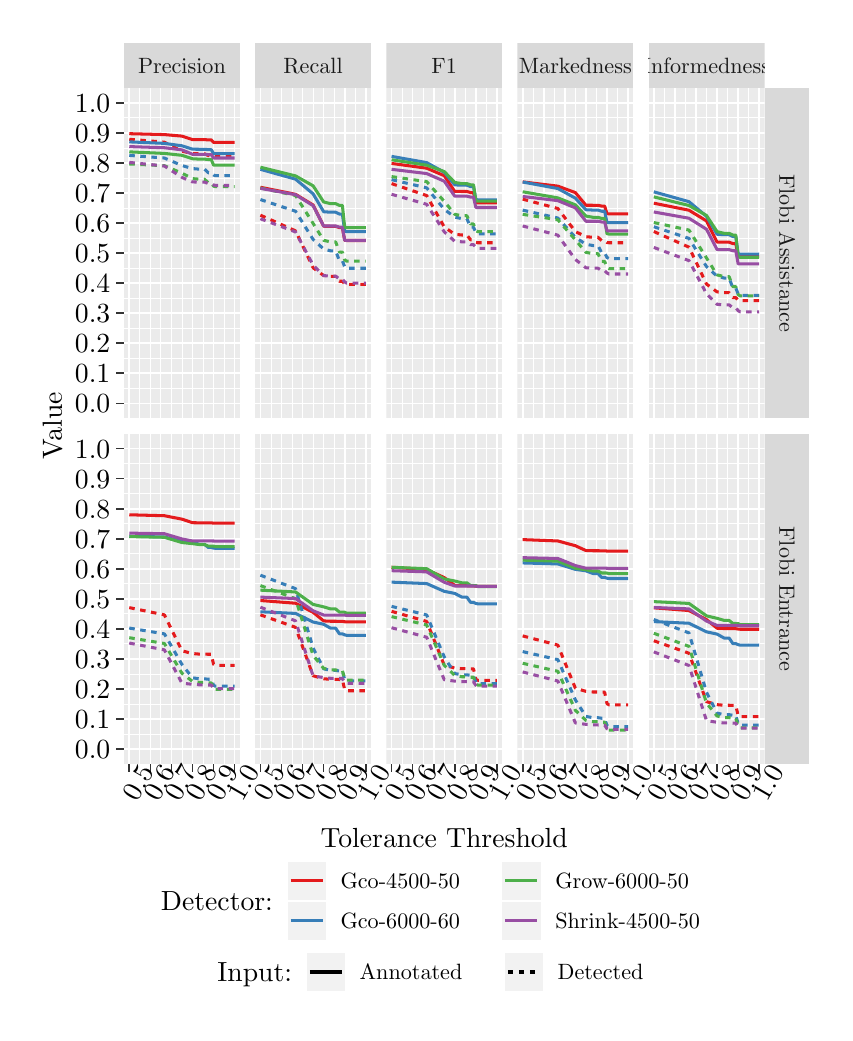
\begin{tikzpicture}[x=1pt,y=1pt]
\definecolor{fillColor}{RGB}{255,255,255}
\path[use as bounding box,fill=fillColor,fill opacity=0.00] (0,0) rectangle (288.00,355.97);
\begin{scope}
\path[clip] (  0.00,  0.00) rectangle (288.00,355.97);
\definecolor{drawColor}{RGB}{255,255,255}
\definecolor{fillColor}{RGB}{255,255,255}

\path[draw=drawColor,line width= 0.6pt,line join=round,line cap=round,fill=fillColor] (  0.00,  0.00) rectangle (288.00,355.97);
\end{scope}
\begin{scope}
\path[clip] ( 34.81,214.79) rectangle ( 76.69,334.21);
\definecolor{fillColor}{gray}{0.92}

\path[fill=fillColor] ( 34.81,214.79) rectangle ( 76.69,334.21);
\definecolor{drawColor}{RGB}{255,255,255}

\path[draw=drawColor,line width= 0.3pt,line join=round] ( 34.81,225.65) --
	( 76.69,225.65);

\path[draw=drawColor,line width= 0.3pt,line join=round] ( 34.81,236.51) --
	( 76.69,236.51);

\path[draw=drawColor,line width= 0.3pt,line join=round] ( 34.81,247.36) --
	( 76.69,247.36);

\path[draw=drawColor,line width= 0.3pt,line join=round] ( 34.81,258.22) --
	( 76.69,258.22);

\path[draw=drawColor,line width= 0.3pt,line join=round] ( 34.81,269.08) --
	( 76.69,269.08);

\path[draw=drawColor,line width= 0.3pt,line join=round] ( 34.81,279.93) --
	( 76.69,279.93);

\path[draw=drawColor,line width= 0.3pt,line join=round] ( 34.81,290.79) --
	( 76.69,290.79);

\path[draw=drawColor,line width= 0.3pt,line join=round] ( 34.81,301.64) --
	( 76.69,301.64);

\path[draw=drawColor,line width= 0.3pt,line join=round] ( 34.81,312.50) --
	( 76.69,312.50);

\path[draw=drawColor,line width= 0.3pt,line join=round] ( 34.81,323.36) --
	( 76.69,323.36);

\path[draw=drawColor,line width= 0.3pt,line join=round] ( 40.52,214.79) --
	( 40.52,334.21);

\path[draw=drawColor,line width= 0.3pt,line join=round] ( 44.33,214.79) --
	( 44.33,334.21);

\path[draw=drawColor,line width= 0.3pt,line join=round] ( 48.13,214.79) --
	( 48.13,334.21);

\path[draw=drawColor,line width= 0.3pt,line join=round] ( 51.94,214.79) --
	( 51.94,334.21);

\path[draw=drawColor,line width= 0.3pt,line join=round] ( 55.75,214.79) --
	( 55.75,334.21);

\path[draw=drawColor,line width= 0.3pt,line join=round] ( 63.37,214.79) --
	( 63.37,334.21);

\path[draw=drawColor,line width= 0.3pt,line join=round] ( 70.98,214.79) --
	( 70.98,334.21);

\path[draw=drawColor,line width= 0.6pt,line join=round] ( 34.81,220.22) --
	( 76.69,220.22);

\path[draw=drawColor,line width= 0.6pt,line join=round] ( 34.81,231.08) --
	( 76.69,231.08);

\path[draw=drawColor,line width= 0.6pt,line join=round] ( 34.81,241.93) --
	( 76.69,241.93);

\path[draw=drawColor,line width= 0.6pt,line join=round] ( 34.81,252.79) --
	( 76.69,252.79);

\path[draw=drawColor,line width= 0.6pt,line join=round] ( 34.81,263.65) --
	( 76.69,263.65);

\path[draw=drawColor,line width= 0.6pt,line join=round] ( 34.81,274.50) --
	( 76.69,274.50);

\path[draw=drawColor,line width= 0.6pt,line join=round] ( 34.81,285.36) --
	( 76.69,285.36);

\path[draw=drawColor,line width= 0.6pt,line join=round] ( 34.81,296.22) --
	( 76.69,296.22);

\path[draw=drawColor,line width= 0.6pt,line join=round] ( 34.81,307.07) --
	( 76.69,307.07);

\path[draw=drawColor,line width= 0.6pt,line join=round] ( 34.81,317.93) --
	( 76.69,317.93);

\path[draw=drawColor,line width= 0.6pt,line join=round] ( 34.81,328.79) --
	( 76.69,328.79);

\path[draw=drawColor,line width= 0.6pt,line join=round] ( 36.71,214.79) --
	( 36.71,334.21);

\path[draw=drawColor,line width= 0.6pt,line join=round] ( 44.33,214.79) --
	( 44.33,334.21);

\path[draw=drawColor,line width= 0.6pt,line join=round] ( 51.94,214.79) --
	( 51.94,334.21);

\path[draw=drawColor,line width= 0.6pt,line join=round] ( 59.56,214.79) --
	( 59.56,334.21);

\path[draw=drawColor,line width= 0.6pt,line join=round] ( 67.17,214.79) --
	( 67.17,334.21);

\path[draw=drawColor,line width= 0.6pt,line join=round] ( 74.79,214.79) --
	( 74.79,334.21);
\definecolor{drawColor}{RGB}{228,26,28}

\path[draw=drawColor,line width= 1.1pt,line join=round] ( 36.71,317.66) --
	( 49.40,317.33) --
	( 55.75,316.78) --
	( 59.56,315.52) --
	( 62.10,315.51) --
	( 63.91,315.51) --
	( 65.27,315.42) --
	( 66.33,315.42) --
	( 67.17,314.52) --
	( 67.87,314.50) --
	( 68.44,314.50) --
	( 74.78,314.50);

\path[draw=drawColor,line width= 1.1pt,dash pattern=on 2pt off 2pt ,line join=round] ( 36.71,315.64) --
	( 49.40,314.60) --
	( 55.75,311.35) --
	( 59.56,310.47) --
	( 62.10,310.38) --
	( 63.91,310.38) --
	( 65.27,309.76) --
	( 66.33,309.76) --
	( 67.17,309.42) --
	( 67.87,309.36) --
	( 68.44,309.36) --
	( 74.78,309.36);
\definecolor{drawColor}{RGB}{55,126,184}

\path[draw=drawColor,line width= 1.1pt,line join=round] ( 36.71,314.70) --
	( 49.40,314.16) --
	( 55.75,313.28) --
	( 59.56,312.06) --
	( 62.10,312.02) --
	( 63.91,312.02) --
	( 65.27,311.89) --
	( 66.33,311.89) --
	( 67.17,310.47) --
	( 67.87,310.45) --
	( 68.44,310.45) --
	( 74.78,310.45);

\path[draw=drawColor,line width= 1.1pt,dash pattern=on 2pt off 2pt ,line join=round] ( 36.71,309.81) --
	( 49.40,308.86) --
	( 55.75,306.15) --
	( 59.56,305.05) --
	( 62.10,304.83) --
	( 63.91,304.83) --
	( 65.27,303.54) --
	( 66.33,303.54) --
	( 67.17,302.70) --
	( 67.87,302.49) --
	( 68.44,302.49) --
	( 74.78,302.49);
\definecolor{drawColor}{RGB}{77,175,74}

\path[draw=drawColor,line width= 1.1pt,line join=round] ( 36.71,311.09) --
	( 49.40,310.53) --
	( 55.75,309.84) --
	( 59.56,308.60) --
	( 62.10,308.46) --
	( 63.91,308.46) --
	( 65.27,308.32) --
	( 66.33,308.32) --
	( 67.17,306.30) --
	( 67.87,306.27) --
	( 68.44,306.27) --
	( 74.78,306.27);

\path[draw=drawColor,line width= 1.1pt,dash pattern=on 2pt off 2pt ,line join=round] ( 36.71,306.72) --
	( 49.40,306.09) --
	( 55.75,303.39) --
	( 59.56,301.42) --
	( 62.10,301.21) --
	( 63.91,301.21) --
	( 65.27,299.86) --
	( 66.33,299.86) --
	( 67.17,298.71) --
	( 67.87,298.52) --
	( 68.44,298.52) --
	( 74.78,298.52);
\definecolor{drawColor}{RGB}{152,78,163}

\path[draw=drawColor,line width= 1.1pt,line join=round] ( 36.71,312.99) --
	( 49.40,312.58) --
	( 55.75,311.82) --
	( 59.56,310.21) --
	( 62.10,310.21) --
	( 63.91,310.21) --
	( 65.27,310.11) --
	( 66.33,310.11) --
	( 67.17,308.87) --
	( 67.87,308.87) --
	( 68.44,308.87) --
	( 74.78,308.87);

\path[draw=drawColor,line width= 1.1pt,dash pattern=on 2pt off 2pt ,line join=round] ( 36.71,307.29) --
	( 49.40,305.98) --
	( 55.75,301.86) --
	( 59.56,300.23) --
	( 62.10,300.15) --
	( 63.91,300.15) --
	( 65.27,299.64) --
	( 66.33,299.64) --
	( 67.17,299.15) --
	( 67.87,298.94) --
	( 68.44,298.94) --
	( 74.78,298.94);
\end{scope}
\begin{scope}
\path[clip] ( 34.81, 89.87) rectangle ( 76.69,209.29);
\definecolor{fillColor}{gray}{0.92}

\path[fill=fillColor] ( 34.81, 89.87) rectangle ( 76.69,209.29);
\definecolor{drawColor}{RGB}{255,255,255}

\path[draw=drawColor,line width= 0.3pt,line join=round] ( 34.81,100.73) --
	( 76.69,100.73);

\path[draw=drawColor,line width= 0.3pt,line join=round] ( 34.81,111.58) --
	( 76.69,111.58);

\path[draw=drawColor,line width= 0.3pt,line join=round] ( 34.81,122.44) --
	( 76.69,122.44);

\path[draw=drawColor,line width= 0.3pt,line join=round] ( 34.81,133.30) --
	( 76.69,133.30);

\path[draw=drawColor,line width= 0.3pt,line join=round] ( 34.81,144.15) --
	( 76.69,144.15);

\path[draw=drawColor,line width= 0.3pt,line join=round] ( 34.81,155.01) --
	( 76.69,155.01);

\path[draw=drawColor,line width= 0.3pt,line join=round] ( 34.81,165.87) --
	( 76.69,165.87);

\path[draw=drawColor,line width= 0.3pt,line join=round] ( 34.81,176.72) --
	( 76.69,176.72);

\path[draw=drawColor,line width= 0.3pt,line join=round] ( 34.81,187.58) --
	( 76.69,187.58);

\path[draw=drawColor,line width= 0.3pt,line join=round] ( 34.81,198.44) --
	( 76.69,198.44);

\path[draw=drawColor,line width= 0.3pt,line join=round] ( 40.52, 89.87) --
	( 40.52,209.29);

\path[draw=drawColor,line width= 0.3pt,line join=round] ( 44.33, 89.87) --
	( 44.33,209.29);

\path[draw=drawColor,line width= 0.3pt,line join=round] ( 48.13, 89.87) --
	( 48.13,209.29);

\path[draw=drawColor,line width= 0.3pt,line join=round] ( 51.94, 89.87) --
	( 51.94,209.29);

\path[draw=drawColor,line width= 0.3pt,line join=round] ( 55.75, 89.87) --
	( 55.75,209.29);

\path[draw=drawColor,line width= 0.3pt,line join=round] ( 63.37, 89.87) --
	( 63.37,209.29);

\path[draw=drawColor,line width= 0.3pt,line join=round] ( 70.98, 89.87) --
	( 70.98,209.29);

\path[draw=drawColor,line width= 0.6pt,line join=round] ( 34.81, 95.30) --
	( 76.69, 95.30);

\path[draw=drawColor,line width= 0.6pt,line join=round] ( 34.81,106.16) --
	( 76.69,106.16);

\path[draw=drawColor,line width= 0.6pt,line join=round] ( 34.81,117.01) --
	( 76.69,117.01);

\path[draw=drawColor,line width= 0.6pt,line join=round] ( 34.81,127.87) --
	( 76.69,127.87);

\path[draw=drawColor,line width= 0.6pt,line join=round] ( 34.81,138.73) --
	( 76.69,138.73);

\path[draw=drawColor,line width= 0.6pt,line join=round] ( 34.81,149.58) --
	( 76.69,149.58);

\path[draw=drawColor,line width= 0.6pt,line join=round] ( 34.81,160.44) --
	( 76.69,160.44);

\path[draw=drawColor,line width= 0.6pt,line join=round] ( 34.81,171.30) --
	( 76.69,171.30);

\path[draw=drawColor,line width= 0.6pt,line join=round] ( 34.81,182.15) --
	( 76.69,182.15);

\path[draw=drawColor,line width= 0.6pt,line join=round] ( 34.81,193.01) --
	( 76.69,193.01);

\path[draw=drawColor,line width= 0.6pt,line join=round] ( 34.81,203.86) --
	( 76.69,203.86);

\path[draw=drawColor,line width= 0.6pt,line join=round] ( 36.71, 89.87) --
	( 36.71,209.29);

\path[draw=drawColor,line width= 0.6pt,line join=round] ( 44.33, 89.87) --
	( 44.33,209.29);

\path[draw=drawColor,line width= 0.6pt,line join=round] ( 51.94, 89.87) --
	( 51.94,209.29);

\path[draw=drawColor,line width= 0.6pt,line join=round] ( 59.56, 89.87) --
	( 59.56,209.29);

\path[draw=drawColor,line width= 0.6pt,line join=round] ( 67.17, 89.87) --
	( 67.17,209.29);

\path[draw=drawColor,line width= 0.6pt,line join=round] ( 74.79, 89.87) --
	( 74.79,209.29);
\definecolor{drawColor}{RGB}{228,26,28}

\path[draw=drawColor,line width= 1.1pt,line join=round] ( 36.71,179.95) --
	( 49.40,179.61) --
	( 55.75,178.37) --
	( 59.56,177.09) --
	( 62.10,177.04) --
	( 63.91,177.04) --
	( 65.27,177.01) --
	( 66.33,177.01) --
	( 67.17,176.95) --
	( 67.87,176.92) --
	( 68.44,176.92) --
	( 74.78,176.92);

\path[draw=drawColor,line width= 1.1pt,dash pattern=on 2pt off 2pt ,line join=round] ( 36.71,146.40) --
	( 49.40,143.78) --
	( 55.75,130.79) --
	( 59.56,129.81) --
	( 62.10,129.60) --
	( 63.91,129.60) --
	( 65.27,129.55) --
	( 66.33,129.55) --
	( 67.17,125.91) --
	( 67.87,125.57) --
	( 68.44,125.57) --
	( 74.78,125.57);
\definecolor{drawColor}{RGB}{55,126,184}

\path[draw=drawColor,line width= 1.1pt,line join=round] ( 36.71,172.20) --
	( 49.40,171.93) --
	( 55.75,170.43) --
	( 59.56,170.02) --
	( 62.10,169.26) --
	( 63.91,169.26) --
	( 65.27,168.14) --
	( 66.33,168.14) --
	( 67.17,167.91) --
	( 67.87,167.83) --
	( 68.44,167.83) --
	( 74.78,167.83);

\path[draw=drawColor,line width= 1.1pt,dash pattern=on 2pt off 2pt ,line join=round] ( 36.71,139.01) --
	( 49.40,136.92) --
	( 55.75,125.86) --
	( 59.56,121.05) --
	( 62.10,120.68) --
	( 63.91,120.68) --
	( 65.27,120.52) --
	( 66.33,120.52) --
	( 67.17,118.35) --
	( 67.87,118.01) --
	( 68.44,118.01) --
	( 74.78,118.01);
\definecolor{drawColor}{RGB}{77,175,74}

\path[draw=drawColor,line width= 1.1pt,line join=round] ( 36.71,172.07) --
	( 49.40,171.82) --
	( 55.75,169.92) --
	( 59.56,169.52) --
	( 62.10,169.18) --
	( 63.91,169.18) --
	( 65.27,168.64) --
	( 66.33,168.64) --
	( 67.17,168.62) --
	( 67.87,168.44) --
	( 68.44,168.44) --
	( 74.78,168.44);

\path[draw=drawColor,line width= 1.1pt,dash pattern=on 2pt off 2pt ,line join=round] ( 36.71,135.53) --
	( 49.40,133.44) --
	( 55.75,122.68) --
	( 59.56,119.74) --
	( 62.10,119.37) --
	( 63.91,119.37) --
	( 65.27,119.22) --
	( 66.33,119.22) --
	( 67.17,117.21) --
	( 67.87,116.88) --
	( 68.44,116.88) --
	( 74.78,116.88);
\definecolor{drawColor}{RGB}{152,78,163}

\path[draw=drawColor,line width= 1.1pt,line join=round] ( 36.71,173.32) --
	( 49.40,173.11) --
	( 55.75,171.21) --
	( 59.56,170.49) --
	( 62.10,170.49) --
	( 63.91,170.49) --
	( 65.27,170.49) --
	( 66.33,170.49) --
	( 67.17,170.48) --
	( 67.87,170.43) --
	( 68.44,170.43) --
	( 74.78,170.43);

\path[draw=drawColor,line width= 1.1pt,dash pattern=on 2pt off 2pt ,line join=round] ( 36.71,133.60) --
	( 49.40,131.14) --
	( 55.75,119.10) --
	( 59.56,118.69) --
	( 62.10,118.51) --
	( 63.91,118.51) --
	( 65.27,118.45) --
	( 66.33,118.45) --
	( 67.17,117.37) --
	( 67.87,117.17) --
	( 68.44,117.17) --
	( 74.78,117.17);
\end{scope}
\begin{scope}
\path[clip] ( 82.19,214.79) rectangle (124.08,334.21);
\definecolor{fillColor}{gray}{0.92}

\path[fill=fillColor] ( 82.19,214.79) rectangle (124.08,334.21);
\definecolor{drawColor}{RGB}{255,255,255}

\path[draw=drawColor,line width= 0.3pt,line join=round] ( 82.19,225.65) --
	(124.08,225.65);

\path[draw=drawColor,line width= 0.3pt,line join=round] ( 82.19,236.51) --
	(124.08,236.51);

\path[draw=drawColor,line width= 0.3pt,line join=round] ( 82.19,247.36) --
	(124.08,247.36);

\path[draw=drawColor,line width= 0.3pt,line join=round] ( 82.19,258.22) --
	(124.08,258.22);

\path[draw=drawColor,line width= 0.3pt,line join=round] ( 82.19,269.08) --
	(124.08,269.08);

\path[draw=drawColor,line width= 0.3pt,line join=round] ( 82.19,279.93) --
	(124.08,279.93);

\path[draw=drawColor,line width= 0.3pt,line join=round] ( 82.19,290.79) --
	(124.08,290.79);

\path[draw=drawColor,line width= 0.3pt,line join=round] ( 82.19,301.64) --
	(124.08,301.64);

\path[draw=drawColor,line width= 0.3pt,line join=round] ( 82.19,312.50) --
	(124.08,312.50);

\path[draw=drawColor,line width= 0.3pt,line join=round] ( 82.19,323.36) --
	(124.08,323.36);

\path[draw=drawColor,line width= 0.3pt,line join=round] ( 87.91,214.79) --
	( 87.91,334.21);

\path[draw=drawColor,line width= 0.3pt,line join=round] ( 91.71,214.79) --
	( 91.71,334.21);

\path[draw=drawColor,line width= 0.3pt,line join=round] ( 95.52,214.79) --
	( 95.52,334.21);

\path[draw=drawColor,line width= 0.3pt,line join=round] ( 99.33,214.79) --
	( 99.33,334.21);

\path[draw=drawColor,line width= 0.3pt,line join=round] (103.14,214.79) --
	(103.14,334.21);

\path[draw=drawColor,line width= 0.3pt,line join=round] (110.75,214.79) --
	(110.75,334.21);

\path[draw=drawColor,line width= 0.3pt,line join=round] (118.37,214.79) --
	(118.37,334.21);

\path[draw=drawColor,line width= 0.6pt,line join=round] ( 82.19,220.22) --
	(124.08,220.22);

\path[draw=drawColor,line width= 0.6pt,line join=round] ( 82.19,231.08) --
	(124.08,231.08);

\path[draw=drawColor,line width= 0.6pt,line join=round] ( 82.19,241.93) --
	(124.08,241.93);

\path[draw=drawColor,line width= 0.6pt,line join=round] ( 82.19,252.79) --
	(124.08,252.79);

\path[draw=drawColor,line width= 0.6pt,line join=round] ( 82.19,263.65) --
	(124.08,263.65);

\path[draw=drawColor,line width= 0.6pt,line join=round] ( 82.19,274.50) --
	(124.08,274.50);

\path[draw=drawColor,line width= 0.6pt,line join=round] ( 82.19,285.36) --
	(124.08,285.36);

\path[draw=drawColor,line width= 0.6pt,line join=round] ( 82.19,296.22) --
	(124.08,296.22);

\path[draw=drawColor,line width= 0.6pt,line join=round] ( 82.19,307.07) --
	(124.08,307.07);

\path[draw=drawColor,line width= 0.6pt,line join=round] ( 82.19,317.93) --
	(124.08,317.93);

\path[draw=drawColor,line width= 0.6pt,line join=round] ( 82.19,328.79) --
	(124.08,328.79);

\path[draw=drawColor,line width= 0.6pt,line join=round] ( 84.10,214.79) --
	( 84.10,334.21);

\path[draw=drawColor,line width= 0.6pt,line join=round] ( 91.71,214.79) --
	( 91.71,334.21);

\path[draw=drawColor,line width= 0.6pt,line join=round] ( 99.33,214.79) --
	( 99.33,334.21);

\path[draw=drawColor,line width= 0.6pt,line join=round] (106.95,214.79) --
	(106.95,334.21);

\path[draw=drawColor,line width= 0.6pt,line join=round] (114.56,214.79) --
	(114.56,334.21);

\path[draw=drawColor,line width= 0.6pt,line join=round] (122.18,214.79) --
	(122.18,334.21);
\definecolor{drawColor}{RGB}{228,26,28}

\path[draw=drawColor,line width= 1.1pt,line join=round] ( 84.10,298.30) --
	( 96.79,295.75) --
	(103.14,291.88) --
	(106.95,284.22) --
	(109.48,284.20) --
	(111.30,284.20) --
	(112.66,283.70) --
	(113.72,283.70) --
	(114.56,279.14) --
	(115.25,279.06) --
	(115.83,279.06) --
	(122.17,279.06);

\path[draw=drawColor,line width= 1.1pt,dash pattern=on 2pt off 2pt ,line join=round] ( 84.10,288.21) --
	( 96.79,282.55) --
	(103.14,269.21) --
	(106.95,266.39) --
	(109.48,266.12) --
	(111.30,266.12) --
	(112.66,264.33) --
	(113.72,264.33) --
	(114.56,263.37) --
	(115.25,263.23) --
	(115.83,263.23) --
	(122.17,263.23);
\definecolor{drawColor}{RGB}{55,126,184}

\path[draw=drawColor,line width= 1.1pt,line join=round] ( 84.10,304.78) --
	( 96.79,301.23) --
	(103.14,295.92) --
	(106.95,289.46) --
	(109.48,289.28) --
	(111.30,289.28) --
	(112.66,288.62) --
	(113.72,288.62) --
	(114.56,282.35) --
	(115.25,282.30) --
	(115.83,282.30) --
	(122.17,282.30);

\path[draw=drawColor,line width= 1.1pt,dash pattern=on 2pt off 2pt ,line join=round] ( 84.10,293.85) --
	( 96.79,289.64) --
	(103.14,279.44) --
	(106.95,275.98) --
	(109.48,275.32) --
	(111.30,275.32) --
	(112.66,271.70) --
	(113.72,271.70) --
	(114.56,269.54) --
	(115.25,269.03) --
	(115.83,269.03) --
	(122.17,269.03);
\definecolor{drawColor}{RGB}{77,175,74}

\path[draw=drawColor,line width= 1.1pt,line join=round] ( 84.10,305.54) --
	( 96.79,302.41) --
	(103.14,298.82) --
	(106.95,292.99) --
	(109.48,292.37) --
	(111.30,292.37) --
	(112.66,291.75) --
	(113.72,291.75) --
	(114.56,283.81) --
	(115.25,283.71) --
	(115.83,283.71) --
	(122.17,283.71);

\path[draw=drawColor,line width= 1.1pt,dash pattern=on 2pt off 2pt ,line join=round] ( 84.10,298.04) --
	( 96.79,295.32) --
	(103.14,285.24) --
	(106.95,279.13) --
	(109.48,278.53) --
	(111.30,278.53) --
	(112.66,274.88) --
	(113.72,274.88) --
	(114.56,272.02) --
	(115.25,271.58) --
	(115.83,271.58) --
	(122.17,271.58);
\definecolor{drawColor}{RGB}{152,78,163}

\path[draw=drawColor,line width= 1.1pt,line join=round] ( 84.10,297.90) --
	( 96.79,295.62) --
	(103.14,291.65) --
	(106.95,284.30) --
	(109.48,284.30) --
	(111.30,284.30) --
	(112.66,283.87) --
	(113.72,283.87) --
	(114.56,279.11) --
	(115.25,279.11) --
	(115.83,279.11) --
	(122.17,279.11);

\path[draw=drawColor,line width= 1.1pt,dash pattern=on 2pt off 2pt ,line join=round] ( 84.10,286.93) --
	( 96.79,282.16) --
	(103.14,270.17) --
	(106.95,266.37) --
	(109.48,266.19) --
	(111.30,266.19) --
	(112.66,265.11) --
	(113.72,265.11) --
	(114.56,264.09) --
	(115.25,263.67) --
	(115.83,263.67) --
	(122.17,263.67);
\end{scope}
\begin{scope}
\path[clip] ( 82.19, 89.87) rectangle (124.08,209.29);
\definecolor{fillColor}{gray}{0.92}

\path[fill=fillColor] ( 82.19, 89.87) rectangle (124.08,209.29);
\definecolor{drawColor}{RGB}{255,255,255}

\path[draw=drawColor,line width= 0.3pt,line join=round] ( 82.19,100.73) --
	(124.08,100.73);

\path[draw=drawColor,line width= 0.3pt,line join=round] ( 82.19,111.58) --
	(124.08,111.58);

\path[draw=drawColor,line width= 0.3pt,line join=round] ( 82.19,122.44) --
	(124.08,122.44);

\path[draw=drawColor,line width= 0.3pt,line join=round] ( 82.19,133.30) --
	(124.08,133.30);

\path[draw=drawColor,line width= 0.3pt,line join=round] ( 82.19,144.15) --
	(124.08,144.15);

\path[draw=drawColor,line width= 0.3pt,line join=round] ( 82.19,155.01) --
	(124.08,155.01);

\path[draw=drawColor,line width= 0.3pt,line join=round] ( 82.19,165.87) --
	(124.08,165.87);

\path[draw=drawColor,line width= 0.3pt,line join=round] ( 82.19,176.72) --
	(124.08,176.72);

\path[draw=drawColor,line width= 0.3pt,line join=round] ( 82.19,187.58) --
	(124.08,187.58);

\path[draw=drawColor,line width= 0.3pt,line join=round] ( 82.19,198.44) --
	(124.08,198.44);

\path[draw=drawColor,line width= 0.3pt,line join=round] ( 87.91, 89.87) --
	( 87.91,209.29);

\path[draw=drawColor,line width= 0.3pt,line join=round] ( 91.71, 89.87) --
	( 91.71,209.29);

\path[draw=drawColor,line width= 0.3pt,line join=round] ( 95.52, 89.87) --
	( 95.52,209.29);

\path[draw=drawColor,line width= 0.3pt,line join=round] ( 99.33, 89.87) --
	( 99.33,209.29);

\path[draw=drawColor,line width= 0.3pt,line join=round] (103.14, 89.87) --
	(103.14,209.29);

\path[draw=drawColor,line width= 0.3pt,line join=round] (110.75, 89.87) --
	(110.75,209.29);

\path[draw=drawColor,line width= 0.3pt,line join=round] (118.37, 89.87) --
	(118.37,209.29);

\path[draw=drawColor,line width= 0.6pt,line join=round] ( 82.19, 95.30) --
	(124.08, 95.30);

\path[draw=drawColor,line width= 0.6pt,line join=round] ( 82.19,106.16) --
	(124.08,106.16);

\path[draw=drawColor,line width= 0.6pt,line join=round] ( 82.19,117.01) --
	(124.08,117.01);

\path[draw=drawColor,line width= 0.6pt,line join=round] ( 82.19,127.87) --
	(124.08,127.87);

\path[draw=drawColor,line width= 0.6pt,line join=round] ( 82.19,138.73) --
	(124.08,138.73);

\path[draw=drawColor,line width= 0.6pt,line join=round] ( 82.19,149.58) --
	(124.08,149.58);

\path[draw=drawColor,line width= 0.6pt,line join=round] ( 82.19,160.44) --
	(124.08,160.44);

\path[draw=drawColor,line width= 0.6pt,line join=round] ( 82.19,171.30) --
	(124.08,171.30);

\path[draw=drawColor,line width= 0.6pt,line join=round] ( 82.19,182.15) --
	(124.08,182.15);

\path[draw=drawColor,line width= 0.6pt,line join=round] ( 82.19,193.01) --
	(124.08,193.01);

\path[draw=drawColor,line width= 0.6pt,line join=round] ( 82.19,203.86) --
	(124.08,203.86);

\path[draw=drawColor,line width= 0.6pt,line join=round] ( 84.10, 89.87) --
	( 84.10,209.29);

\path[draw=drawColor,line width= 0.6pt,line join=round] ( 91.71, 89.87) --
	( 91.71,209.29);

\path[draw=drawColor,line width= 0.6pt,line join=round] ( 99.33, 89.87) --
	( 99.33,209.29);

\path[draw=drawColor,line width= 0.6pt,line join=round] (106.95, 89.87) --
	(106.95,209.29);

\path[draw=drawColor,line width= 0.6pt,line join=round] (114.56, 89.87) --
	(114.56,209.29);

\path[draw=drawColor,line width= 0.6pt,line join=round] (122.18, 89.87) --
	(122.18,209.29);
\definecolor{drawColor}{RGB}{228,26,28}

\path[draw=drawColor,line width= 1.1pt,line join=round] ( 84.10,148.97) --
	( 96.79,147.99) --
	(103.14,144.70) --
	(106.95,141.60) --
	(109.48,141.48) --
	(111.30,141.48) --
	(112.66,141.43) --
	(113.72,141.43) --
	(114.56,141.30) --
	(115.25,141.22) --
	(115.83,141.22) --
	(122.17,141.22);

\path[draw=drawColor,line width= 1.1pt,dash pattern=on 2pt off 2pt ,line join=round] ( 84.10,143.79) --
	( 96.79,139.29) --
	(103.14,121.78) --
	(106.95,120.70) --
	(109.48,120.48) --
	(111.30,120.48) --
	(112.66,120.43) --
	(113.72,120.43) --
	(114.56,116.71) --
	(115.25,116.37) --
	(115.83,116.37) --
	(122.17,116.37);
\definecolor{drawColor}{RGB}{55,126,184}

\path[draw=drawColor,line width= 1.1pt,line join=round] ( 84.10,144.90) --
	( 96.79,144.31) --
	(103.14,141.20) --
	(106.95,140.39) --
	(109.48,138.96) --
	(111.30,138.96) --
	(112.66,136.94) --
	(113.72,136.94) --
	(114.56,136.55) --
	(115.25,136.41) --
	(115.83,136.41) --
	(122.17,136.41);

\path[draw=drawColor,line width= 1.1pt,dash pattern=on 2pt off 2pt ,line join=round] ( 84.10,158.12) --
	( 96.79,153.26) --
	(103.14,131.82) --
	(106.95,124.29) --
	(109.48,123.73) --
	(111.30,123.73) --
	(112.66,123.50) --
	(113.72,123.50) --
	(114.56,120.43) --
	(115.25,119.96) --
	(115.83,119.96) --
	(122.17,119.96);
\definecolor{drawColor}{RGB}{77,175,74}

\path[draw=drawColor,line width= 1.1pt,line join=round] ( 84.10,152.71) --
	( 96.79,152.06) --
	(103.14,147.56) --
	(106.95,146.68) --
	(109.48,145.93) --
	(111.30,145.93) --
	(112.66,144.79) --
	(113.72,144.79) --
	(114.56,144.76) --
	(115.25,144.38) --
	(115.83,144.38) --
	(122.17,144.38);

\path[draw=drawColor,line width= 1.1pt,dash pattern=on 2pt off 2pt ,line join=round] ( 84.10,154.36) --
	( 96.79,149.63) --
	(103.14,129.13) --
	(106.95,124.45) --
	(109.48,123.88) --
	(111.30,123.88) --
	(112.66,123.65) --
	(113.72,123.65) --
	(114.56,120.66) --
	(115.25,120.19) --
	(115.83,120.19) --
	(122.17,120.19);
\definecolor{drawColor}{RGB}{152,78,163}

\path[draw=drawColor,line width= 1.1pt,line join=round] ( 84.10,150.20) --
	( 96.79,149.68) --
	(103.14,145.26) --
	(106.95,143.72) --
	(109.48,143.72) --
	(111.30,143.72) --
	(112.66,143.72) --
	(113.72,143.72) --
	(114.56,143.69) --
	(115.25,143.59) --
	(115.83,143.59) --
	(122.17,143.59);

\path[draw=drawColor,line width= 1.1pt,dash pattern=on 2pt off 2pt ,line join=round] ( 84.10,146.56) --
	( 96.79,141.63) --
	(103.14,121.71) --
	(106.95,121.13) --
	(109.48,120.86) --
	(111.30,120.86) --
	(112.66,120.79) --
	(113.72,120.79) --
	(114.56,119.29) --
	(115.25,119.03) --
	(115.83,119.03) --
	(122.17,119.03);
\end{scope}
\begin{scope}
\path[clip] (129.58,214.79) rectangle (171.47,334.21);
\definecolor{fillColor}{gray}{0.92}

\path[fill=fillColor] (129.58,214.79) rectangle (171.47,334.21);
\definecolor{drawColor}{RGB}{255,255,255}

\path[draw=drawColor,line width= 0.3pt,line join=round] (129.58,225.65) --
	(171.47,225.65);

\path[draw=drawColor,line width= 0.3pt,line join=round] (129.58,236.51) --
	(171.47,236.51);

\path[draw=drawColor,line width= 0.3pt,line join=round] (129.58,247.36) --
	(171.47,247.36);

\path[draw=drawColor,line width= 0.3pt,line join=round] (129.58,258.22) --
	(171.47,258.22);

\path[draw=drawColor,line width= 0.3pt,line join=round] (129.58,269.08) --
	(171.47,269.08);

\path[draw=drawColor,line width= 0.3pt,line join=round] (129.58,279.93) --
	(171.47,279.93);

\path[draw=drawColor,line width= 0.3pt,line join=round] (129.58,290.79) --
	(171.47,290.79);

\path[draw=drawColor,line width= 0.3pt,line join=round] (129.58,301.64) --
	(171.47,301.64);

\path[draw=drawColor,line width= 0.3pt,line join=round] (129.58,312.50) --
	(171.47,312.50);

\path[draw=drawColor,line width= 0.3pt,line join=round] (129.58,323.36) --
	(171.47,323.36);

\path[draw=drawColor,line width= 0.3pt,line join=round] (135.29,214.79) --
	(135.29,334.21);

\path[draw=drawColor,line width= 0.3pt,line join=round] (139.10,214.79) --
	(139.10,334.21);

\path[draw=drawColor,line width= 0.3pt,line join=round] (142.91,214.79) --
	(142.91,334.21);

\path[draw=drawColor,line width= 0.3pt,line join=round] (146.72,214.79) --
	(146.72,334.21);

\path[draw=drawColor,line width= 0.3pt,line join=round] (150.53,214.79) --
	(150.53,334.21);

\path[draw=drawColor,line width= 0.3pt,line join=round] (158.14,214.79) --
	(158.14,334.21);

\path[draw=drawColor,line width= 0.3pt,line join=round] (165.76,214.79) --
	(165.76,334.21);

\path[draw=drawColor,line width= 0.6pt,line join=round] (129.58,220.22) --
	(171.47,220.22);

\path[draw=drawColor,line width= 0.6pt,line join=round] (129.58,231.08) --
	(171.47,231.08);

\path[draw=drawColor,line width= 0.6pt,line join=round] (129.58,241.93) --
	(171.47,241.93);

\path[draw=drawColor,line width= 0.6pt,line join=round] (129.58,252.79) --
	(171.47,252.79);

\path[draw=drawColor,line width= 0.6pt,line join=round] (129.58,263.65) --
	(171.47,263.65);

\path[draw=drawColor,line width= 0.6pt,line join=round] (129.58,274.50) --
	(171.47,274.50);

\path[draw=drawColor,line width= 0.6pt,line join=round] (129.58,285.36) --
	(171.47,285.36);

\path[draw=drawColor,line width= 0.6pt,line join=round] (129.58,296.22) --
	(171.47,296.22);

\path[draw=drawColor,line width= 0.6pt,line join=round] (129.58,307.07) --
	(171.47,307.07);

\path[draw=drawColor,line width= 0.6pt,line join=round] (129.58,317.93) --
	(171.47,317.93);

\path[draw=drawColor,line width= 0.6pt,line join=round] (129.58,328.79) --
	(171.47,328.79);

\path[draw=drawColor,line width= 0.6pt,line join=round] (131.49,214.79) --
	(131.49,334.21);

\path[draw=drawColor,line width= 0.6pt,line join=round] (139.10,214.79) --
	(139.10,334.21);

\path[draw=drawColor,line width= 0.6pt,line join=round] (146.72,214.79) --
	(146.72,334.21);

\path[draw=drawColor,line width= 0.6pt,line join=round] (154.33,214.79) --
	(154.33,334.21);

\path[draw=drawColor,line width= 0.6pt,line join=round] (161.95,214.79) --
	(161.95,334.21);

\path[draw=drawColor,line width= 0.6pt,line join=round] (169.57,214.79) --
	(169.57,334.21);
\definecolor{drawColor}{RGB}{228,26,28}

\path[draw=drawColor,line width= 1.1pt,line join=round] (131.49,306.91) --
	(144.18,305.19) --
	(150.53,302.48) --
	(154.33,296.80) --
	(156.87,296.77) --
	(158.69,296.77) --
	(160.05,296.39) --
	(161.10,296.39) --
	(161.95,292.75) --
	(162.64,292.68) --
	(163.22,292.68) --
	(169.56,292.68);

\path[draw=drawColor,line width= 1.1pt,dash pattern=on 2pt off 2pt ,line join=round] (131.49,299.62) --
	(144.18,295.30) --
	(150.53,283.94) --
	(154.33,281.30) --
	(156.87,281.05) --
	(158.69,281.05) --
	(160.05,279.32) --
	(161.10,279.32) --
	(161.95,278.39) --
	(162.64,278.24) --
	(163.22,278.24) --
	(169.56,278.24);
\definecolor{drawColor}{RGB}{55,126,184}

\path[draw=drawColor,line width= 1.1pt,line join=round] (131.49,309.46) --
	(144.18,307.21) --
	(150.53,303.71) --
	(154.33,299.17) --
	(156.87,299.04) --
	(158.69,299.04) --
	(160.05,298.56) --
	(161.10,298.56) --
	(161.95,293.82) --
	(162.64,293.77) --
	(163.22,293.77) --
	(169.56,293.77);

\path[draw=drawColor,line width= 1.1pt,dash pattern=on 2pt off 2pt ,line join=round] (131.49,301.05) --
	(144.18,298.08) --
	(150.53,290.34) --
	(154.33,287.51) --
	(156.87,286.96) --
	(158.69,286.96) --
	(160.05,283.86) --
	(161.10,283.86) --
	(161.95,281.94) --
	(162.64,281.49) --
	(163.22,281.49) --
	(169.56,281.49);
\definecolor{drawColor}{RGB}{77,175,74}

\path[draw=drawColor,line width= 1.1pt,line join=round] (131.49,308.23) --
	(144.18,306.28) --
	(150.53,303.97) --
	(154.33,300.04) --
	(156.87,299.61) --
	(158.69,299.61) --
	(160.05,299.18) --
	(161.10,299.18) --
	(161.95,293.37) --
	(162.64,293.28) --
	(163.22,293.28) --
	(169.56,293.28);

\path[draw=drawColor,line width= 1.1pt,dash pattern=on 2pt off 2pt ,line join=round] (131.49,302.15) --
	(144.18,300.34) --
	(150.53,293.20) --
	(154.33,288.50) --
	(156.87,288.03) --
	(158.69,288.03) --
	(160.05,285.05) --
	(161.10,285.05) --
	(161.95,282.63) --
	(162.64,282.25) --
	(163.22,282.25) --
	(169.56,282.25);
\definecolor{drawColor}{RGB}{152,78,163}

\path[draw=drawColor,line width= 1.1pt,line join=round] (131.49,304.78) --
	(144.18,303.25) --
	(150.53,300.49) --
	(154.33,295.08) --
	(156.87,295.08) --
	(158.69,295.08) --
	(160.05,294.75) --
	(161.10,294.75) --
	(161.95,290.99) --
	(162.64,290.99) --
	(163.22,290.99) --
	(169.56,290.99);

\path[draw=drawColor,line width= 1.1pt,dash pattern=on 2pt off 2pt ,line join=round] (131.49,295.76) --
	(144.18,292.15) --
	(150.53,282.20) --
	(154.33,278.76) --
	(156.87,278.59) --
	(158.69,278.59) --
	(160.05,277.58) --
	(161.10,277.58) --
	(161.95,276.61) --
	(162.64,276.21) --
	(163.22,276.21) --
	(169.56,276.21);
\end{scope}
\begin{scope}
\path[clip] (129.58, 89.87) rectangle (171.47,209.29);
\definecolor{fillColor}{gray}{0.92}

\path[fill=fillColor] (129.58, 89.87) rectangle (171.47,209.29);
\definecolor{drawColor}{RGB}{255,255,255}

\path[draw=drawColor,line width= 0.3pt,line join=round] (129.58,100.73) --
	(171.47,100.73);

\path[draw=drawColor,line width= 0.3pt,line join=round] (129.58,111.58) --
	(171.47,111.58);

\path[draw=drawColor,line width= 0.3pt,line join=round] (129.58,122.44) --
	(171.47,122.44);

\path[draw=drawColor,line width= 0.3pt,line join=round] (129.58,133.30) --
	(171.47,133.30);

\path[draw=drawColor,line width= 0.3pt,line join=round] (129.58,144.15) --
	(171.47,144.15);

\path[draw=drawColor,line width= 0.3pt,line join=round] (129.58,155.01) --
	(171.47,155.01);

\path[draw=drawColor,line width= 0.3pt,line join=round] (129.58,165.87) --
	(171.47,165.87);

\path[draw=drawColor,line width= 0.3pt,line join=round] (129.58,176.72) --
	(171.47,176.72);

\path[draw=drawColor,line width= 0.3pt,line join=round] (129.58,187.58) --
	(171.47,187.58);

\path[draw=drawColor,line width= 0.3pt,line join=round] (129.58,198.44) --
	(171.47,198.44);

\path[draw=drawColor,line width= 0.3pt,line join=round] (135.29, 89.87) --
	(135.29,209.29);

\path[draw=drawColor,line width= 0.3pt,line join=round] (139.10, 89.87) --
	(139.10,209.29);

\path[draw=drawColor,line width= 0.3pt,line join=round] (142.91, 89.87) --
	(142.91,209.29);

\path[draw=drawColor,line width= 0.3pt,line join=round] (146.72, 89.87) --
	(146.72,209.29);

\path[draw=drawColor,line width= 0.3pt,line join=round] (150.53, 89.87) --
	(150.53,209.29);

\path[draw=drawColor,line width= 0.3pt,line join=round] (158.14, 89.87) --
	(158.14,209.29);

\path[draw=drawColor,line width= 0.3pt,line join=round] (165.76, 89.87) --
	(165.76,209.29);

\path[draw=drawColor,line width= 0.6pt,line join=round] (129.58, 95.30) --
	(171.47, 95.30);

\path[draw=drawColor,line width= 0.6pt,line join=round] (129.58,106.16) --
	(171.47,106.16);

\path[draw=drawColor,line width= 0.6pt,line join=round] (129.58,117.01) --
	(171.47,117.01);

\path[draw=drawColor,line width= 0.6pt,line join=round] (129.58,127.87) --
	(171.47,127.87);

\path[draw=drawColor,line width= 0.6pt,line join=round] (129.58,138.73) --
	(171.47,138.73);

\path[draw=drawColor,line width= 0.6pt,line join=round] (129.58,149.58) --
	(171.47,149.58);

\path[draw=drawColor,line width= 0.6pt,line join=round] (129.58,160.44) --
	(171.47,160.44);

\path[draw=drawColor,line width= 0.6pt,line join=round] (129.58,171.30) --
	(171.47,171.30);

\path[draw=drawColor,line width= 0.6pt,line join=round] (129.58,182.15) --
	(171.47,182.15);

\path[draw=drawColor,line width= 0.6pt,line join=round] (129.58,193.01) --
	(171.47,193.01);

\path[draw=drawColor,line width= 0.6pt,line join=round] (129.58,203.86) --
	(171.47,203.86);

\path[draw=drawColor,line width= 0.6pt,line join=round] (131.49, 89.87) --
	(131.49,209.29);

\path[draw=drawColor,line width= 0.6pt,line join=round] (139.10, 89.87) --
	(139.10,209.29);

\path[draw=drawColor,line width= 0.6pt,line join=round] (146.72, 89.87) --
	(146.72,209.29);

\path[draw=drawColor,line width= 0.6pt,line join=round] (154.33, 89.87) --
	(154.33,209.29);

\path[draw=drawColor,line width= 0.6pt,line join=round] (161.95, 89.87) --
	(161.95,209.29);

\path[draw=drawColor,line width= 0.6pt,line join=round] (169.57, 89.87) --
	(169.57,209.29);
\definecolor{drawColor}{RGB}{228,26,28}

\path[draw=drawColor,line width= 1.1pt,line join=round] (131.49,160.99) --
	(144.18,160.15) --
	(150.53,157.26) --
	(154.33,154.43) --
	(156.87,154.32) --
	(158.69,154.32) --
	(160.05,154.27) --
	(161.10,154.27) --
	(161.95,154.14) --
	(162.64,154.08) --
	(163.22,154.08) --
	(169.56,154.08);

\path[draw=drawColor,line width= 1.1pt,dash pattern=on 2pt off 2pt ,line join=round] (131.49,145.06) --
	(144.18,141.42) --
	(150.53,125.63) --
	(154.33,124.56) --
	(156.87,124.34) --
	(158.69,124.34) --
	(160.05,124.29) --
	(161.10,124.29) --
	(161.95,120.50) --
	(162.64,120.15) --
	(163.22,120.15) --
	(169.56,120.15);
\definecolor{drawColor}{RGB}{55,126,184}

\path[draw=drawColor,line width= 1.1pt,line join=round] (131.49,155.61) --
	(144.18,155.09) --
	(150.53,152.28) --
	(154.33,151.54) --
	(156.87,150.21) --
	(158.69,150.21) --
	(160.05,148.29) --
	(161.10,148.29) --
	(161.95,147.91) --
	(162.64,147.77) --
	(163.22,147.77) --
	(169.56,147.77);

\path[draw=drawColor,line width= 1.1pt,dash pattern=on 2pt off 2pt ,line join=round] (131.49,146.85) --
	(144.18,143.75) --
	(150.53,128.58) --
	(154.33,122.58) --
	(156.87,122.12) --
	(158.69,122.12) --
	(160.05,121.93) --
	(161.10,121.93) --
	(161.95,119.34) --
	(162.64,118.95) --
	(163.22,118.95) --
	(169.56,118.95);
\definecolor{drawColor}{RGB}{77,175,74}

\path[draw=drawColor,line width= 1.1pt,line join=round] (131.49,160.99) --
	(144.18,160.47) --
	(150.53,156.77) --
	(154.33,156.02) --
	(156.87,155.38) --
	(158.69,155.38) --
	(160.05,154.40) --
	(161.10,154.40) --
	(161.95,154.37) --
	(162.64,154.04) --
	(163.22,154.04) --
	(169.56,154.04);

\path[draw=drawColor,line width= 1.1pt,dash pattern=on 2pt off 2pt ,line join=round] (131.49,143.16) --
	(144.18,140.12) --
	(150.53,125.56) --
	(154.33,121.89) --
	(156.87,121.43) --
	(158.69,121.43) --
	(160.05,121.25) --
	(161.10,121.25) --
	(161.95,118.81) --
	(162.64,118.42) --
	(163.22,118.42) --
	(169.56,118.42);
\definecolor{drawColor}{RGB}{152,78,163}

\path[draw=drawColor,line width= 1.1pt,line join=round] (131.49,159.75) --
	(144.18,159.32) --
	(150.53,155.56) --
	(154.33,154.21) --
	(156.87,154.21) --
	(158.69,154.21) --
	(160.05,154.21) --
	(161.10,154.21) --
	(161.95,154.18) --
	(162.64,154.09) --
	(163.22,154.09) --
	(169.56,154.09);

\path[draw=drawColor,line width= 1.1pt,dash pattern=on 2pt off 2pt ,line join=round] (131.49,139.14) --
	(144.18,135.71) --
	(150.53,120.34) --
	(154.33,119.85) --
	(156.87,119.63) --
	(158.69,119.63) --
	(160.05,119.57) --
	(161.10,119.57) --
	(161.95,118.29) --
	(162.64,118.06) --
	(163.22,118.06) --
	(169.56,118.06);
\end{scope}
\begin{scope}
\path[clip] (176.97,214.79) rectangle (218.86,334.21);
\definecolor{fillColor}{gray}{0.92}

\path[fill=fillColor] (176.97,214.79) rectangle (218.86,334.21);
\definecolor{drawColor}{RGB}{255,255,255}

\path[draw=drawColor,line width= 0.3pt,line join=round] (176.97,225.65) --
	(218.86,225.65);

\path[draw=drawColor,line width= 0.3pt,line join=round] (176.97,236.51) --
	(218.86,236.51);

\path[draw=drawColor,line width= 0.3pt,line join=round] (176.97,247.36) --
	(218.86,247.36);

\path[draw=drawColor,line width= 0.3pt,line join=round] (176.97,258.22) --
	(218.86,258.22);

\path[draw=drawColor,line width= 0.3pt,line join=round] (176.97,269.08) --
	(218.86,269.08);

\path[draw=drawColor,line width= 0.3pt,line join=round] (176.97,279.93) --
	(218.86,279.93);

\path[draw=drawColor,line width= 0.3pt,line join=round] (176.97,290.79) --
	(218.86,290.79);

\path[draw=drawColor,line width= 0.3pt,line join=round] (176.97,301.64) --
	(218.86,301.64);

\path[draw=drawColor,line width= 0.3pt,line join=round] (176.97,312.50) --
	(218.86,312.50);

\path[draw=drawColor,line width= 0.3pt,line join=round] (176.97,323.36) --
	(218.86,323.36);

\path[draw=drawColor,line width= 0.3pt,line join=round] (182.68,214.79) --
	(182.68,334.21);

\path[draw=drawColor,line width= 0.3pt,line join=round] (186.49,214.79) --
	(186.49,334.21);

\path[draw=drawColor,line width= 0.3pt,line join=round] (190.30,214.79) --
	(190.30,334.21);

\path[draw=drawColor,line width= 0.3pt,line join=round] (194.11,214.79) --
	(194.11,334.21);

\path[draw=drawColor,line width= 0.3pt,line join=round] (197.91,214.79) --
	(197.91,334.21);

\path[draw=drawColor,line width= 0.3pt,line join=round] (205.53,214.79) --
	(205.53,334.21);

\path[draw=drawColor,line width= 0.3pt,line join=round] (213.15,214.79) --
	(213.15,334.21);

\path[draw=drawColor,line width= 0.6pt,line join=round] (176.97,220.22) --
	(218.86,220.22);

\path[draw=drawColor,line width= 0.6pt,line join=round] (176.97,231.08) --
	(218.86,231.08);

\path[draw=drawColor,line width= 0.6pt,line join=round] (176.97,241.93) --
	(218.86,241.93);

\path[draw=drawColor,line width= 0.6pt,line join=round] (176.97,252.79) --
	(218.86,252.79);

\path[draw=drawColor,line width= 0.6pt,line join=round] (176.97,263.65) --
	(218.86,263.65);

\path[draw=drawColor,line width= 0.6pt,line join=round] (176.97,274.50) --
	(218.86,274.50);

\path[draw=drawColor,line width= 0.6pt,line join=round] (176.97,285.36) --
	(218.86,285.36);

\path[draw=drawColor,line width= 0.6pt,line join=round] (176.97,296.22) --
	(218.86,296.22);

\path[draw=drawColor,line width= 0.6pt,line join=round] (176.97,307.07) --
	(218.86,307.07);

\path[draw=drawColor,line width= 0.6pt,line join=round] (176.97,317.93) --
	(218.86,317.93);

\path[draw=drawColor,line width= 0.6pt,line join=round] (176.97,328.79) --
	(218.86,328.79);

\path[draw=drawColor,line width= 0.6pt,line join=round] (178.87,214.79) --
	(178.87,334.21);

\path[draw=drawColor,line width= 0.6pt,line join=round] (186.49,214.79) --
	(186.49,334.21);

\path[draw=drawColor,line width= 0.6pt,line join=round] (194.11,214.79) --
	(194.11,334.21);

\path[draw=drawColor,line width= 0.6pt,line join=round] (201.72,214.79) --
	(201.72,334.21);

\path[draw=drawColor,line width= 0.6pt,line join=round] (209.34,214.79) --
	(209.34,334.21);

\path[draw=drawColor,line width= 0.6pt,line join=round] (216.95,214.79) --
	(216.95,334.21);
\definecolor{drawColor}{RGB}{228,26,28}

\path[draw=drawColor,line width= 1.1pt,line join=round] (178.87,300.24) --
	(191.57,298.70) --
	(197.91,296.37) --
	(201.72,291.80) --
	(204.26,291.79) --
	(206.07,291.79) --
	(207.43,291.49) --
	(208.49,291.49) --
	(209.34,288.75) --
	(210.03,288.70) --
	(210.61,288.70) --
	(216.95,288.70);

\path[draw=drawColor,line width= 1.1pt,dash pattern=on 2pt off 2pt ,line join=round] (178.87,294.01) --
	(191.57,290.62) --
	(197.91,282.30) --
	(201.72,280.42) --
	(204.26,280.24) --
	(206.07,280.24) --
	(207.43,279.01) --
	(208.49,279.01) --
	(209.34,278.34) --
	(210.03,278.24) --
	(210.61,278.24) --
	(216.95,278.24);
\definecolor{drawColor}{RGB}{55,126,184}

\path[draw=drawColor,line width= 1.1pt,line join=round] (178.87,300.20) --
	(191.57,297.84) --
	(197.91,294.36) --
	(201.72,290.17) --
	(204.26,290.06) --
	(206.07,290.06) --
	(207.43,289.63) --
	(208.49,289.63) --
	(209.34,285.54) --
	(210.03,285.50) --
	(210.61,285.50) --
	(216.95,285.50);

\path[draw=drawColor,line width= 1.1pt,dash pattern=on 2pt off 2pt ,line join=round] (178.87,290.03) --
	(191.57,287.18) --
	(197.91,280.17) --
	(201.72,277.71) --
	(204.26,277.23) --
	(206.07,277.23) --
	(207.43,274.57) --
	(208.49,274.57) --
	(209.34,272.93) --
	(210.03,272.54) --
	(210.61,272.54) --
	(216.95,272.54);
\definecolor{drawColor}{RGB}{77,175,74}

\path[draw=drawColor,line width= 1.1pt,line join=round] (178.87,296.67) --
	(191.57,294.46) --
	(197.91,291.94) --
	(201.72,287.88) --
	(204.26,287.45) --
	(206.07,287.45) --
	(207.43,287.02) --
	(208.49,287.02) --
	(209.34,281.48) --
	(210.03,281.40) --
	(210.61,281.40) --
	(216.95,281.40);

\path[draw=drawColor,line width= 1.1pt,dash pattern=on 2pt off 2pt ,line join=round] (178.87,288.52) --
	(191.57,286.56) --
	(197.91,279.29) --
	(201.72,274.77) --
	(204.26,274.32) --
	(206.07,274.32) --
	(207.43,271.52) --
	(208.49,271.52) --
	(209.34,269.27) --
	(210.03,268.92) --
	(210.61,268.92) --
	(216.95,268.92);
\definecolor{drawColor}{RGB}{152,78,163}

\path[draw=drawColor,line width= 1.1pt,line join=round] (178.87,294.97) --
	(191.57,293.47) --
	(197.91,290.85) --
	(201.72,286.02) --
	(204.26,286.02) --
	(206.07,286.02) --
	(207.43,285.73) --
	(208.49,285.73) --
	(209.34,282.54) --
	(210.03,282.54) --
	(210.61,282.54) --
	(216.95,282.54);

\path[draw=drawColor,line width= 1.1pt,dash pattern=on 2pt off 2pt ,line join=round] (178.87,284.31) --
	(191.57,280.99) --
	(197.91,272.20) --
	(201.72,269.20) --
	(204.26,269.05) --
	(206.07,269.05) --
	(207.43,268.17) --
	(208.49,268.17) --
	(209.34,267.32) --
	(210.03,266.96) --
	(210.61,266.96) --
	(216.95,266.96);
\end{scope}
\begin{scope}
\path[clip] (176.97, 89.87) rectangle (218.86,209.29);
\definecolor{fillColor}{gray}{0.92}

\path[fill=fillColor] (176.97, 89.87) rectangle (218.86,209.29);
\definecolor{drawColor}{RGB}{255,255,255}

\path[draw=drawColor,line width= 0.3pt,line join=round] (176.97,100.73) --
	(218.86,100.73);

\path[draw=drawColor,line width= 0.3pt,line join=round] (176.97,111.58) --
	(218.86,111.58);

\path[draw=drawColor,line width= 0.3pt,line join=round] (176.97,122.44) --
	(218.86,122.44);

\path[draw=drawColor,line width= 0.3pt,line join=round] (176.97,133.30) --
	(218.86,133.30);

\path[draw=drawColor,line width= 0.3pt,line join=round] (176.97,144.15) --
	(218.86,144.15);

\path[draw=drawColor,line width= 0.3pt,line join=round] (176.97,155.01) --
	(218.86,155.01);

\path[draw=drawColor,line width= 0.3pt,line join=round] (176.97,165.87) --
	(218.86,165.87);

\path[draw=drawColor,line width= 0.3pt,line join=round] (176.97,176.72) --
	(218.86,176.72);

\path[draw=drawColor,line width= 0.3pt,line join=round] (176.97,187.58) --
	(218.86,187.58);

\path[draw=drawColor,line width= 0.3pt,line join=round] (176.97,198.44) --
	(218.86,198.44);

\path[draw=drawColor,line width= 0.3pt,line join=round] (182.68, 89.87) --
	(182.68,209.29);

\path[draw=drawColor,line width= 0.3pt,line join=round] (186.49, 89.87) --
	(186.49,209.29);

\path[draw=drawColor,line width= 0.3pt,line join=round] (190.30, 89.87) --
	(190.30,209.29);

\path[draw=drawColor,line width= 0.3pt,line join=round] (194.11, 89.87) --
	(194.11,209.29);

\path[draw=drawColor,line width= 0.3pt,line join=round] (197.91, 89.87) --
	(197.91,209.29);

\path[draw=drawColor,line width= 0.3pt,line join=round] (205.53, 89.87) --
	(205.53,209.29);

\path[draw=drawColor,line width= 0.3pt,line join=round] (213.15, 89.87) --
	(213.15,209.29);

\path[draw=drawColor,line width= 0.6pt,line join=round] (176.97, 95.30) --
	(218.86, 95.30);

\path[draw=drawColor,line width= 0.6pt,line join=round] (176.97,106.16) --
	(218.86,106.16);

\path[draw=drawColor,line width= 0.6pt,line join=round] (176.97,117.01) --
	(218.86,117.01);

\path[draw=drawColor,line width= 0.6pt,line join=round] (176.97,127.87) --
	(218.86,127.87);

\path[draw=drawColor,line width= 0.6pt,line join=round] (176.97,138.73) --
	(218.86,138.73);

\path[draw=drawColor,line width= 0.6pt,line join=round] (176.97,149.58) --
	(218.86,149.58);

\path[draw=drawColor,line width= 0.6pt,line join=round] (176.97,160.44) --
	(218.86,160.44);

\path[draw=drawColor,line width= 0.6pt,line join=round] (176.97,171.30) --
	(218.86,171.30);

\path[draw=drawColor,line width= 0.6pt,line join=round] (176.97,182.15) --
	(218.86,182.15);

\path[draw=drawColor,line width= 0.6pt,line join=round] (176.97,193.01) --
	(218.86,193.01);

\path[draw=drawColor,line width= 0.6pt,line join=round] (176.97,203.86) --
	(218.86,203.86);

\path[draw=drawColor,line width= 0.6pt,line join=round] (178.87, 89.87) --
	(178.87,209.29);

\path[draw=drawColor,line width= 0.6pt,line join=round] (186.49, 89.87) --
	(186.49,209.29);

\path[draw=drawColor,line width= 0.6pt,line join=round] (194.11, 89.87) --
	(194.11,209.29);

\path[draw=drawColor,line width= 0.6pt,line join=round] (201.72, 89.87) --
	(201.72,209.29);

\path[draw=drawColor,line width= 0.6pt,line join=round] (209.34, 89.87) --
	(209.34,209.29);

\path[draw=drawColor,line width= 0.6pt,line join=round] (216.95, 89.87) --
	(216.95,209.29);
\definecolor{drawColor}{RGB}{228,26,28}

\path[draw=drawColor,line width= 1.1pt,line join=round] (178.87,170.98) --
	(191.57,170.49) --
	(197.91,168.77) --
	(201.72,167.02) --
	(204.26,166.96) --
	(206.07,166.96) --
	(207.43,166.92) --
	(208.49,166.92) --
	(209.34,166.85) --
	(210.03,166.80) --
	(210.61,166.80) --
	(216.95,166.80);

\path[draw=drawColor,line width= 1.1pt,dash pattern=on 2pt off 2pt ,line join=round] (178.87,136.18) --
	(191.57,132.86) --
	(197.91,117.29) --
	(201.72,116.15) --
	(204.26,115.91) --
	(206.07,115.91) --
	(207.43,115.85) --
	(208.49,115.85) --
	(209.34,111.68) --
	(210.03,111.29) --
	(210.61,111.29) --
	(216.95,111.29);
\definecolor{drawColor}{RGB}{55,126,184}

\path[draw=drawColor,line width= 1.1pt,line join=round] (178.87,162.55) --
	(191.57,162.19) --
	(197.91,160.23) --
	(201.72,159.70) --
	(204.26,158.73) --
	(206.07,158.73) --
	(207.43,157.31) --
	(208.49,157.31) --
	(209.34,157.03) --
	(210.03,156.93) --
	(210.61,156.93) --
	(216.95,156.93);

\path[draw=drawColor,line width= 1.1pt,dash pattern=on 2pt off 2pt ,line join=round] (178.87,130.51) --
	(191.57,127.61) --
	(197.91,113.06) --
	(201.72,107.09) --
	(204.26,106.63) --
	(206.07,106.63) --
	(207.43,106.43) --
	(208.49,106.43) --
	(209.34,103.80) --
	(210.03,103.39) --
	(210.61,103.39) --
	(216.95,103.39);
\definecolor{drawColor}{RGB}{77,175,74}

\path[draw=drawColor,line width= 1.1pt,line join=round] (178.87,163.56) --
	(191.57,163.20) --
	(197.91,160.62) --
	(201.72,160.09) --
	(204.26,159.63) --
	(206.07,159.63) --
	(207.43,158.92) --
	(208.49,158.92) --
	(209.34,158.90) --
	(210.03,158.66) --
	(210.61,158.66) --
	(216.95,158.66);

\path[draw=drawColor,line width= 1.1pt,dash pattern=on 2pt off 2pt ,line join=round] (178.87,126.29) --
	(191.57,123.40) --
	(197.91,109.30) --
	(201.72,105.64) --
	(204.26,105.18) --
	(206.07,105.18) --
	(207.43,104.99) --
	(208.49,104.99) --
	(209.34,102.52) --
	(210.03,102.13) --
	(210.61,102.13) --
	(216.95,102.13);
\definecolor{drawColor}{RGB}{152,78,163}

\path[draw=drawColor,line width= 1.1pt,line join=round] (178.87,164.45) --
	(191.57,164.16) --
	(197.91,161.60) --
	(201.72,160.65) --
	(204.26,160.65) --
	(206.07,160.65) --
	(207.43,160.65) --
	(208.49,160.65) --
	(209.34,160.63) --
	(210.03,160.57) --
	(210.61,160.57) --
	(216.95,160.57);

\path[draw=drawColor,line width= 1.1pt,dash pattern=on 2pt off 2pt ,line join=round] (178.87,123.16) --
	(191.57,119.88) --
	(197.91,104.73) --
	(201.72,104.23) --
	(204.26,104.00) --
	(206.07,104.00) --
	(207.43,103.94) --
	(208.49,103.94) --
	(209.34,102.63) --
	(210.03,102.39) --
	(210.61,102.39) --
	(216.95,102.39);
\end{scope}
\begin{scope}
\path[clip] (224.36,214.79) rectangle (266.25,334.21);
\definecolor{fillColor}{gray}{0.92}

\path[fill=fillColor] (224.36,214.79) rectangle (266.25,334.21);
\definecolor{drawColor}{RGB}{255,255,255}

\path[draw=drawColor,line width= 0.3pt,line join=round] (224.36,225.65) --
	(266.25,225.65);

\path[draw=drawColor,line width= 0.3pt,line join=round] (224.36,236.51) --
	(266.25,236.51);

\path[draw=drawColor,line width= 0.3pt,line join=round] (224.36,247.36) --
	(266.25,247.36);

\path[draw=drawColor,line width= 0.3pt,line join=round] (224.36,258.22) --
	(266.25,258.22);

\path[draw=drawColor,line width= 0.3pt,line join=round] (224.36,269.08) --
	(266.25,269.08);

\path[draw=drawColor,line width= 0.3pt,line join=round] (224.36,279.93) --
	(266.25,279.93);

\path[draw=drawColor,line width= 0.3pt,line join=round] (224.36,290.79) --
	(266.25,290.79);

\path[draw=drawColor,line width= 0.3pt,line join=round] (224.36,301.64) --
	(266.25,301.64);

\path[draw=drawColor,line width= 0.3pt,line join=round] (224.36,312.50) --
	(266.25,312.50);

\path[draw=drawColor,line width= 0.3pt,line join=round] (224.36,323.36) --
	(266.25,323.36);

\path[draw=drawColor,line width= 0.3pt,line join=round] (230.07,214.79) --
	(230.07,334.21);

\path[draw=drawColor,line width= 0.3pt,line join=round] (233.88,214.79) --
	(233.88,334.21);

\path[draw=drawColor,line width= 0.3pt,line join=round] (237.69,214.79) --
	(237.69,334.21);

\path[draw=drawColor,line width= 0.3pt,line join=round] (241.49,214.79) --
	(241.49,334.21);

\path[draw=drawColor,line width= 0.3pt,line join=round] (245.30,214.79) --
	(245.30,334.21);

\path[draw=drawColor,line width= 0.3pt,line join=round] (252.92,214.79) --
	(252.92,334.21);

\path[draw=drawColor,line width= 0.3pt,line join=round] (260.53,214.79) --
	(260.53,334.21);

\path[draw=drawColor,line width= 0.6pt,line join=round] (224.36,220.22) --
	(266.25,220.22);

\path[draw=drawColor,line width= 0.6pt,line join=round] (224.36,231.08) --
	(266.25,231.08);

\path[draw=drawColor,line width= 0.6pt,line join=round] (224.36,241.93) --
	(266.25,241.93);

\path[draw=drawColor,line width= 0.6pt,line join=round] (224.36,252.79) --
	(266.25,252.79);

\path[draw=drawColor,line width= 0.6pt,line join=round] (224.36,263.65) --
	(266.25,263.65);

\path[draw=drawColor,line width= 0.6pt,line join=round] (224.36,274.50) --
	(266.25,274.50);

\path[draw=drawColor,line width= 0.6pt,line join=round] (224.36,285.36) --
	(266.25,285.36);

\path[draw=drawColor,line width= 0.6pt,line join=round] (224.36,296.22) --
	(266.25,296.22);

\path[draw=drawColor,line width= 0.6pt,line join=round] (224.36,307.07) --
	(266.25,307.07);

\path[draw=drawColor,line width= 0.6pt,line join=round] (224.36,317.93) --
	(266.25,317.93);

\path[draw=drawColor,line width= 0.6pt,line join=round] (224.36,328.79) --
	(266.25,328.79);

\path[draw=drawColor,line width= 0.6pt,line join=round] (226.26,214.79) --
	(226.26,334.21);

\path[draw=drawColor,line width= 0.6pt,line join=round] (233.88,214.79) --
	(233.88,334.21);

\path[draw=drawColor,line width= 0.6pt,line join=round] (241.49,214.79) --
	(241.49,334.21);

\path[draw=drawColor,line width= 0.6pt,line join=round] (249.11,214.79) --
	(249.11,334.21);

\path[draw=drawColor,line width= 0.6pt,line join=round] (256.73,214.79) --
	(256.73,334.21);

\path[draw=drawColor,line width= 0.6pt,line join=round] (264.34,214.79) --
	(264.34,334.21);
\definecolor{drawColor}{RGB}{228,26,28}

\path[draw=drawColor,line width= 1.1pt,line join=round] (226.26,292.55) --
	(238.96,290.00) --
	(245.30,286.13) --
	(249.11,278.48) --
	(251.65,278.45) --
	(253.46,278.45) --
	(254.82,277.95) --
	(255.88,277.95) --
	(256.73,273.39) --
	(257.42,273.31) --
	(258.00,273.31) --
	(264.33,273.31);

\path[draw=drawColor,line width= 1.1pt,dash pattern=on 2pt off 2pt ,line join=round] (226.26,282.31) --
	(238.96,276.65) --
	(245.30,263.31) --
	(249.11,260.49) --
	(251.65,260.22) --
	(253.46,260.22) --
	(254.82,258.43) --
	(255.88,258.43) --
	(256.73,257.47) --
	(257.42,257.33) --
	(258.00,257.33) --
	(264.33,257.33);
\definecolor{drawColor}{RGB}{55,126,184}

\path[draw=drawColor,line width= 1.1pt,line join=round] (226.26,296.65) --
	(238.96,293.09) --
	(245.30,287.79) --
	(249.11,281.33) --
	(251.65,281.15) --
	(253.46,281.15) --
	(254.82,280.49) --
	(255.88,280.49) --
	(256.73,274.22) --
	(257.42,274.17) --
	(258.00,274.17) --
	(264.33,274.17);

\path[draw=drawColor,line width= 1.1pt,dash pattern=on 2pt off 2pt ,line join=round] (226.26,284.03) --
	(238.96,279.82) --
	(245.30,269.62) --
	(249.11,266.16) --
	(251.65,265.50) --
	(253.46,265.50) --
	(254.82,261.88) --
	(255.88,261.88) --
	(256.73,259.72) --
	(257.42,259.21) --
	(258.00,259.21) --
	(264.33,259.21);
\definecolor{drawColor}{RGB}{77,175,74}

\path[draw=drawColor,line width= 1.1pt,line join=round] (226.26,294.83) --
	(238.96,291.70) --
	(245.30,288.10) --
	(249.11,282.27) --
	(251.65,281.65) --
	(253.46,281.65) --
	(254.82,281.04) --
	(255.88,281.04) --
	(256.73,273.10) --
	(257.42,272.99) --
	(258.00,272.99) --
	(264.33,272.99);

\path[draw=drawColor,line width= 1.1pt,dash pattern=on 2pt off 2pt ,line join=round] (226.26,285.55) --
	(238.96,282.82) --
	(245.30,272.74) --
	(249.11,266.63) --
	(251.65,266.03) --
	(253.46,266.03) --
	(254.82,262.38) --
	(255.88,262.38) --
	(256.73,259.53) --
	(257.42,259.08) --
	(258.00,259.08) --
	(264.33,259.08);
\definecolor{drawColor}{RGB}{152,78,163}

\path[draw=drawColor,line width= 1.1pt,line join=round] (226.26,289.37) --
	(238.96,287.10) --
	(245.30,283.12) --
	(249.11,275.78) --
	(251.65,275.78) --
	(253.46,275.78) --
	(254.82,275.35) --
	(255.88,275.35) --
	(256.73,270.58) --
	(257.42,270.58) --
	(258.00,270.58) --
	(264.33,270.58);

\path[draw=drawColor,line width= 1.1pt,dash pattern=on 2pt off 2pt ,line join=round] (226.26,276.56) --
	(238.96,271.79) --
	(245.30,259.80) --
	(249.11,256.00) --
	(251.65,255.82) --
	(253.46,255.82) --
	(254.82,254.74) --
	(255.88,254.74) --
	(256.73,253.72) --
	(257.42,253.30) --
	(258.00,253.30) --
	(264.33,253.30);
\end{scope}
\begin{scope}
\path[clip] (224.36, 89.87) rectangle (266.25,209.29);
\definecolor{fillColor}{gray}{0.92}

\path[fill=fillColor] (224.36, 89.87) rectangle (266.25,209.29);
\definecolor{drawColor}{RGB}{255,255,255}

\path[draw=drawColor,line width= 0.3pt,line join=round] (224.36,100.73) --
	(266.25,100.73);

\path[draw=drawColor,line width= 0.3pt,line join=round] (224.36,111.58) --
	(266.25,111.58);

\path[draw=drawColor,line width= 0.3pt,line join=round] (224.36,122.44) --
	(266.25,122.44);

\path[draw=drawColor,line width= 0.3pt,line join=round] (224.36,133.30) --
	(266.25,133.30);

\path[draw=drawColor,line width= 0.3pt,line join=round] (224.36,144.15) --
	(266.25,144.15);

\path[draw=drawColor,line width= 0.3pt,line join=round] (224.36,155.01) --
	(266.25,155.01);

\path[draw=drawColor,line width= 0.3pt,line join=round] (224.36,165.87) --
	(266.25,165.87);

\path[draw=drawColor,line width= 0.3pt,line join=round] (224.36,176.72) --
	(266.25,176.72);

\path[draw=drawColor,line width= 0.3pt,line join=round] (224.36,187.58) --
	(266.25,187.58);

\path[draw=drawColor,line width= 0.3pt,line join=round] (224.36,198.44) --
	(266.25,198.44);

\path[draw=drawColor,line width= 0.3pt,line join=round] (230.07, 89.87) --
	(230.07,209.29);

\path[draw=drawColor,line width= 0.3pt,line join=round] (233.88, 89.87) --
	(233.88,209.29);

\path[draw=drawColor,line width= 0.3pt,line join=round] (237.69, 89.87) --
	(237.69,209.29);

\path[draw=drawColor,line width= 0.3pt,line join=round] (241.49, 89.87) --
	(241.49,209.29);

\path[draw=drawColor,line width= 0.3pt,line join=round] (245.30, 89.87) --
	(245.30,209.29);

\path[draw=drawColor,line width= 0.3pt,line join=round] (252.92, 89.87) --
	(252.92,209.29);

\path[draw=drawColor,line width= 0.3pt,line join=round] (260.53, 89.87) --
	(260.53,209.29);

\path[draw=drawColor,line width= 0.6pt,line join=round] (224.36, 95.30) --
	(266.25, 95.30);

\path[draw=drawColor,line width= 0.6pt,line join=round] (224.36,106.16) --
	(266.25,106.16);

\path[draw=drawColor,line width= 0.6pt,line join=round] (224.36,117.01) --
	(266.25,117.01);

\path[draw=drawColor,line width= 0.6pt,line join=round] (224.36,127.87) --
	(266.25,127.87);

\path[draw=drawColor,line width= 0.6pt,line join=round] (224.36,138.73) --
	(266.25,138.73);

\path[draw=drawColor,line width= 0.6pt,line join=round] (224.36,149.58) --
	(266.25,149.58);

\path[draw=drawColor,line width= 0.6pt,line join=round] (224.36,160.44) --
	(266.25,160.44);

\path[draw=drawColor,line width= 0.6pt,line join=round] (224.36,171.30) --
	(266.25,171.30);

\path[draw=drawColor,line width= 0.6pt,line join=round] (224.36,182.15) --
	(266.25,182.15);

\path[draw=drawColor,line width= 0.6pt,line join=round] (224.36,193.01) --
	(266.25,193.01);

\path[draw=drawColor,line width= 0.6pt,line join=round] (224.36,203.86) --
	(266.25,203.86);

\path[draw=drawColor,line width= 0.6pt,line join=round] (226.26, 89.87) --
	(226.26,209.29);

\path[draw=drawColor,line width= 0.6pt,line join=round] (233.88, 89.87) --
	(233.88,209.29);

\path[draw=drawColor,line width= 0.6pt,line join=round] (241.49, 89.87) --
	(241.49,209.29);

\path[draw=drawColor,line width= 0.6pt,line join=round] (249.11, 89.87) --
	(249.11,209.29);

\path[draw=drawColor,line width= 0.6pt,line join=round] (256.73, 89.87) --
	(256.73,209.29);

\path[draw=drawColor,line width= 0.6pt,line join=round] (264.34, 89.87) --
	(264.34,209.29);
\definecolor{drawColor}{RGB}{228,26,28}

\path[draw=drawColor,line width= 1.1pt,line join=round] (226.26,146.33) --
	(238.96,145.35) --
	(245.30,142.07) --
	(249.11,138.96) --
	(251.65,138.85) --
	(253.46,138.85) --
	(254.82,138.79) --
	(255.88,138.79) --
	(256.73,138.66) --
	(257.42,138.59) --
	(258.00,138.59) --
	(264.33,138.59);

\path[draw=drawColor,line width= 1.1pt,dash pattern=on 2pt off 2pt ,line join=round] (226.26,134.43) --
	(238.96,129.92) --
	(245.30,112.42) --
	(249.11,111.34) --
	(251.65,111.12) --
	(253.46,111.12) --
	(254.82,111.07) --
	(255.88,111.07) --
	(256.73,107.35) --
	(257.42,107.01) --
	(258.00,107.01) --
	(264.33,107.01);
\definecolor{drawColor}{RGB}{55,126,184}

\path[draw=drawColor,line width= 1.1pt,line join=round] (226.26,141.35) --
	(238.96,140.76) --
	(245.30,137.65) --
	(249.11,136.84) --
	(251.65,135.41) --
	(253.46,135.41) --
	(254.82,133.39) --
	(255.88,133.39) --
	(256.73,133.00) --
	(257.42,132.86) --
	(258.00,132.86) --
	(264.33,132.86);

\path[draw=drawColor,line width= 1.1pt,dash pattern=on 2pt off 2pt ,line join=round] (226.26,142.11) --
	(238.96,137.26) --
	(245.30,115.82) --
	(249.11,108.28) --
	(251.65,107.73) --
	(253.46,107.73) --
	(254.82,107.50) --
	(255.88,107.50) --
	(256.73,104.42) --
	(257.42,103.95) --
	(258.00,103.95) --
	(264.33,103.95);
\definecolor{drawColor}{RGB}{77,175,74}

\path[draw=drawColor,line width= 1.1pt,line join=round] (226.26,148.57) --
	(238.96,147.92) --
	(245.30,143.42) --
	(249.11,142.54) --
	(251.65,141.79) --
	(253.46,141.79) --
	(254.82,140.66) --
	(255.88,140.66) --
	(256.73,140.63) --
	(257.42,140.25) --
	(258.00,140.25) --
	(264.33,140.25);

\path[draw=drawColor,line width= 1.1pt,dash pattern=on 2pt off 2pt ,line join=round] (226.26,137.13) --
	(238.96,132.41) --
	(245.30,111.90) --
	(249.11,107.23) --
	(251.65,106.66) --
	(253.46,106.66) --
	(254.82,106.42) --
	(255.88,106.42) --
	(256.73,103.44) --
	(257.42,102.97) --
	(258.00,102.97) --
	(264.33,102.97);
\definecolor{drawColor}{RGB}{152,78,163}

\path[draw=drawColor,line width= 1.1pt,line join=round] (226.26,146.46) --
	(238.96,145.94) --
	(245.30,141.53) --
	(249.11,139.98) --
	(251.65,139.98) --
	(253.46,139.98) --
	(254.82,139.98) --
	(255.88,139.98) --
	(256.73,139.96) --
	(257.42,139.85) --
	(258.00,139.85) --
	(264.33,139.85);

\path[draw=drawColor,line width= 1.1pt,dash pattern=on 2pt off 2pt ,line join=round] (226.26,130.41) --
	(238.96,125.49) --
	(245.30,105.56) --
	(249.11,104.98) --
	(251.65,104.72) --
	(253.46,104.72) --
	(254.82,104.65) --
	(255.88,104.65) --
	(256.73,103.14) --
	(257.42,102.88) --
	(258.00,102.88) --
	(264.33,102.88);
\end{scope}
\begin{scope}
\path[clip] ( 34.81,334.21) rectangle ( 76.69,350.47);
\definecolor{fillColor}{gray}{0.85}

\path[fill=fillColor] ( 34.81,334.21) rectangle ( 76.69,350.47);
\definecolor{drawColor}{gray}{0.10}

\node[text=drawColor,anchor=base,inner sep=0pt, outer sep=0pt, scale=  0.80] at ( 55.75,339.59) {Precision};
\end{scope}
\begin{scope}
\path[clip] ( 82.19,334.21) rectangle (124.08,350.47);
\definecolor{fillColor}{gray}{0.85}

\path[fill=fillColor] ( 82.19,334.21) rectangle (124.08,350.47);
\definecolor{drawColor}{gray}{0.10}

\node[text=drawColor,anchor=base,inner sep=0pt, outer sep=0pt, scale=  0.80] at (103.14,339.59) {Recall};
\end{scope}
\begin{scope}
\path[clip] (129.58,334.21) rectangle (171.47,350.47);
\definecolor{fillColor}{gray}{0.85}

\path[fill=fillColor] (129.58,334.21) rectangle (171.47,350.47);
\definecolor{drawColor}{gray}{0.10}

\node[text=drawColor,anchor=base,inner sep=0pt, outer sep=0pt, scale=  0.80] at (150.53,339.59) {F1};
\end{scope}
\begin{scope}
\path[clip] (176.97,334.21) rectangle (218.86,350.47);
\definecolor{fillColor}{gray}{0.85}

\path[fill=fillColor] (176.97,334.21) rectangle (218.86,350.47);
\definecolor{drawColor}{gray}{0.10}

\node[text=drawColor,anchor=base,inner sep=0pt, outer sep=0pt, scale=  0.80] at (197.91,339.59) {Markedness};
\end{scope}
\begin{scope}
\path[clip] (224.36,334.21) rectangle (266.25,350.47);
\definecolor{fillColor}{gray}{0.85}

\path[fill=fillColor] (224.36,334.21) rectangle (266.25,350.47);
\definecolor{drawColor}{gray}{0.10}

\node[text=drawColor,anchor=base,inner sep=0pt, outer sep=0pt, scale=  0.80] at (245.30,339.59) {Informedness};
\end{scope}
\begin{scope}
\path[clip] (266.25,214.79) rectangle (282.50,334.21);
\definecolor{fillColor}{gray}{0.85}

\path[fill=fillColor] (266.25,214.79) rectangle (282.50,334.21);
\definecolor{drawColor}{gray}{0.10}

\node[text=drawColor,rotate=-90.00,anchor=base,inner sep=0pt, outer sep=0pt, scale=  0.80] at (271.62,274.50) {Flobi Assistance};
\end{scope}
\begin{scope}
\path[clip] (266.25, 89.87) rectangle (282.50,209.29);
\definecolor{fillColor}{gray}{0.85}

\path[fill=fillColor] (266.25, 89.87) rectangle (282.50,209.29);
\definecolor{drawColor}{gray}{0.10}

\node[text=drawColor,rotate=-90.00,anchor=base,inner sep=0pt, outer sep=0pt, scale=  0.80] at (271.62,149.58) {Flobi Entrance};
\end{scope}
\begin{scope}
\path[clip] (  0.00,  0.00) rectangle (288.00,355.97);
\definecolor{drawColor}{gray}{0.20}

\path[draw=drawColor,line width= 0.6pt,line join=round] ( 36.71, 87.12) --
	( 36.71, 89.87);

\path[draw=drawColor,line width= 0.6pt,line join=round] ( 44.33, 87.12) --
	( 44.33, 89.87);

\path[draw=drawColor,line width= 0.6pt,line join=round] ( 51.94, 87.12) --
	( 51.94, 89.87);

\path[draw=drawColor,line width= 0.6pt,line join=round] ( 59.56, 87.12) --
	( 59.56, 89.87);

\path[draw=drawColor,line width= 0.6pt,line join=round] ( 67.17, 87.12) --
	( 67.17, 89.87);

\path[draw=drawColor,line width= 0.6pt,line join=round] ( 74.79, 87.12) --
	( 74.79, 89.87);
\end{scope}
\begin{scope}
\path[clip] (  0.00,  0.00) rectangle (288.00,355.97);
\definecolor{drawColor}{RGB}{0,0,0}

\node[text=drawColor,rotate= 60.00,anchor=base,inner sep=0pt, outer sep=0pt, scale=  1.00] at ( 42.67, 81.48) {0.5};

\node[text=drawColor,rotate= 60.00,anchor=base,inner sep=0pt, outer sep=0pt, scale=  1.00] at ( 50.29, 81.48) {0.6};

\node[text=drawColor,rotate= 60.00,anchor=base,inner sep=0pt, outer sep=0pt, scale=  1.00] at ( 57.91, 81.48) {0.7};

\node[text=drawColor,rotate= 60.00,anchor=base,inner sep=0pt, outer sep=0pt, scale=  1.00] at ( 65.52, 81.48) {0.8};

\node[text=drawColor,rotate= 60.00,anchor=base,inner sep=0pt, outer sep=0pt, scale=  1.00] at ( 73.14, 81.48) {0.9};

\node[text=drawColor,rotate= 60.00,anchor=base,inner sep=0pt, outer sep=0pt, scale=  1.00] at ( 80.75, 81.48) {1.0};
\end{scope}
\begin{scope}
\path[clip] (  0.00,  0.00) rectangle (288.00,355.97);
\definecolor{drawColor}{gray}{0.20}

\path[draw=drawColor,line width= 0.6pt,line join=round] ( 84.10, 87.12) --
	( 84.10, 89.87);

\path[draw=drawColor,line width= 0.6pt,line join=round] ( 91.71, 87.12) --
	( 91.71, 89.87);

\path[draw=drawColor,line width= 0.6pt,line join=round] ( 99.33, 87.12) --
	( 99.33, 89.87);

\path[draw=drawColor,line width= 0.6pt,line join=round] (106.95, 87.12) --
	(106.95, 89.87);

\path[draw=drawColor,line width= 0.6pt,line join=round] (114.56, 87.12) --
	(114.56, 89.87);

\path[draw=drawColor,line width= 0.6pt,line join=round] (122.18, 87.12) --
	(122.18, 89.87);
\end{scope}
\begin{scope}
\path[clip] (  0.00,  0.00) rectangle (288.00,355.97);
\definecolor{drawColor}{RGB}{0,0,0}

\node[text=drawColor,rotate= 60.00,anchor=base,inner sep=0pt, outer sep=0pt, scale=  1.00] at ( 90.06, 81.48) {0.5};

\node[text=drawColor,rotate= 60.00,anchor=base,inner sep=0pt, outer sep=0pt, scale=  1.00] at ( 97.68, 81.48) {0.6};

\node[text=drawColor,rotate= 60.00,anchor=base,inner sep=0pt, outer sep=0pt, scale=  1.00] at (105.29, 81.48) {0.7};

\node[text=drawColor,rotate= 60.00,anchor=base,inner sep=0pt, outer sep=0pt, scale=  1.00] at (112.91, 81.48) {0.8};

\node[text=drawColor,rotate= 60.00,anchor=base,inner sep=0pt, outer sep=0pt, scale=  1.00] at (120.53, 81.48) {0.9};

\node[text=drawColor,rotate= 60.00,anchor=base,inner sep=0pt, outer sep=0pt, scale=  1.00] at (128.14, 81.48) {1.0};
\end{scope}
\begin{scope}
\path[clip] (  0.00,  0.00) rectangle (288.00,355.97);
\definecolor{drawColor}{gray}{0.20}

\path[draw=drawColor,line width= 0.6pt,line join=round] (131.49, 87.12) --
	(131.49, 89.87);

\path[draw=drawColor,line width= 0.6pt,line join=round] (139.10, 87.12) --
	(139.10, 89.87);

\path[draw=drawColor,line width= 0.6pt,line join=round] (146.72, 87.12) --
	(146.72, 89.87);

\path[draw=drawColor,line width= 0.6pt,line join=round] (154.33, 87.12) --
	(154.33, 89.87);

\path[draw=drawColor,line width= 0.6pt,line join=round] (161.95, 87.12) --
	(161.95, 89.87);

\path[draw=drawColor,line width= 0.6pt,line join=round] (169.57, 87.12) --
	(169.57, 89.87);
\end{scope}
\begin{scope}
\path[clip] (  0.00,  0.00) rectangle (288.00,355.97);
\definecolor{drawColor}{RGB}{0,0,0}

\node[text=drawColor,rotate= 60.00,anchor=base,inner sep=0pt, outer sep=0pt, scale=  1.00] at (137.45, 81.48) {0.5};

\node[text=drawColor,rotate= 60.00,anchor=base,inner sep=0pt, outer sep=0pt, scale=  1.00] at (145.07, 81.48) {0.6};

\node[text=drawColor,rotate= 60.00,anchor=base,inner sep=0pt, outer sep=0pt, scale=  1.00] at (152.68, 81.48) {0.7};

\node[text=drawColor,rotate= 60.00,anchor=base,inner sep=0pt, outer sep=0pt, scale=  1.00] at (160.30, 81.48) {0.8};

\node[text=drawColor,rotate= 60.00,anchor=base,inner sep=0pt, outer sep=0pt, scale=  1.00] at (167.91, 81.48) {0.9};

\node[text=drawColor,rotate= 60.00,anchor=base,inner sep=0pt, outer sep=0pt, scale=  1.00] at (175.53, 81.48) {1.0};
\end{scope}
\begin{scope}
\path[clip] (  0.00,  0.00) rectangle (288.00,355.97);
\definecolor{drawColor}{gray}{0.20}

\path[draw=drawColor,line width= 0.6pt,line join=round] (178.87, 87.12) --
	(178.87, 89.87);

\path[draw=drawColor,line width= 0.6pt,line join=round] (186.49, 87.12) --
	(186.49, 89.87);

\path[draw=drawColor,line width= 0.6pt,line join=round] (194.11, 87.12) --
	(194.11, 89.87);

\path[draw=drawColor,line width= 0.6pt,line join=round] (201.72, 87.12) --
	(201.72, 89.87);

\path[draw=drawColor,line width= 0.6pt,line join=round] (209.34, 87.12) --
	(209.34, 89.87);

\path[draw=drawColor,line width= 0.6pt,line join=round] (216.95, 87.12) --
	(216.95, 89.87);
\end{scope}
\begin{scope}
\path[clip] (  0.00,  0.00) rectangle (288.00,355.97);
\definecolor{drawColor}{RGB}{0,0,0}

\node[text=drawColor,rotate= 60.00,anchor=base,inner sep=0pt, outer sep=0pt, scale=  1.00] at (184.84, 81.48) {0.5};

\node[text=drawColor,rotate= 60.00,anchor=base,inner sep=0pt, outer sep=0pt, scale=  1.00] at (192.45, 81.48) {0.6};

\node[text=drawColor,rotate= 60.00,anchor=base,inner sep=0pt, outer sep=0pt, scale=  1.00] at (200.07, 81.48) {0.7};

\node[text=drawColor,rotate= 60.00,anchor=base,inner sep=0pt, outer sep=0pt, scale=  1.00] at (207.69, 81.48) {0.8};

\node[text=drawColor,rotate= 60.00,anchor=base,inner sep=0pt, outer sep=0pt, scale=  1.00] at (215.30, 81.48) {0.9};

\node[text=drawColor,rotate= 60.00,anchor=base,inner sep=0pt, outer sep=0pt, scale=  1.00] at (222.92, 81.48) {1.0};
\end{scope}
\begin{scope}
\path[clip] (  0.00,  0.00) rectangle (288.00,355.97);
\definecolor{drawColor}{gray}{0.20}

\path[draw=drawColor,line width= 0.6pt,line join=round] (226.26, 87.12) --
	(226.26, 89.87);

\path[draw=drawColor,line width= 0.6pt,line join=round] (233.88, 87.12) --
	(233.88, 89.87);

\path[draw=drawColor,line width= 0.6pt,line join=round] (241.49, 87.12) --
	(241.49, 89.87);

\path[draw=drawColor,line width= 0.6pt,line join=round] (249.11, 87.12) --
	(249.11, 89.87);

\path[draw=drawColor,line width= 0.6pt,line join=round] (256.73, 87.12) --
	(256.73, 89.87);

\path[draw=drawColor,line width= 0.6pt,line join=round] (264.34, 87.12) --
	(264.34, 89.87);
\end{scope}
\begin{scope}
\path[clip] (  0.00,  0.00) rectangle (288.00,355.97);
\definecolor{drawColor}{RGB}{0,0,0}

\node[text=drawColor,rotate= 60.00,anchor=base,inner sep=0pt, outer sep=0pt, scale=  1.00] at (232.23, 81.48) {0.5};

\node[text=drawColor,rotate= 60.00,anchor=base,inner sep=0pt, outer sep=0pt, scale=  1.00] at (239.84, 81.48) {0.6};

\node[text=drawColor,rotate= 60.00,anchor=base,inner sep=0pt, outer sep=0pt, scale=  1.00] at (247.46, 81.48) {0.7};

\node[text=drawColor,rotate= 60.00,anchor=base,inner sep=0pt, outer sep=0pt, scale=  1.00] at (255.07, 81.48) {0.8};

\node[text=drawColor,rotate= 60.00,anchor=base,inner sep=0pt, outer sep=0pt, scale=  1.00] at (262.69, 81.48) {0.9};

\node[text=drawColor,rotate= 60.00,anchor=base,inner sep=0pt, outer sep=0pt, scale=  1.00] at (270.31, 81.48) {1.0};
\end{scope}
\begin{scope}
\path[clip] (  0.00,  0.00) rectangle (288.00,355.97);
\definecolor{drawColor}{RGB}{0,0,0}

\node[text=drawColor,anchor=base east,inner sep=0pt, outer sep=0pt, scale=  1.00] at ( 29.86,216.78) {0.0};

\node[text=drawColor,anchor=base east,inner sep=0pt, outer sep=0pt, scale=  1.00] at ( 29.86,227.63) {0.1};

\node[text=drawColor,anchor=base east,inner sep=0pt, outer sep=0pt, scale=  1.00] at ( 29.86,238.49) {0.2};

\node[text=drawColor,anchor=base east,inner sep=0pt, outer sep=0pt, scale=  1.00] at ( 29.86,249.35) {0.3};

\node[text=drawColor,anchor=base east,inner sep=0pt, outer sep=0pt, scale=  1.00] at ( 29.86,260.20) {0.4};

\node[text=drawColor,anchor=base east,inner sep=0pt, outer sep=0pt, scale=  1.00] at ( 29.86,271.06) {0.5};

\node[text=drawColor,anchor=base east,inner sep=0pt, outer sep=0pt, scale=  1.00] at ( 29.86,281.92) {0.6};

\node[text=drawColor,anchor=base east,inner sep=0pt, outer sep=0pt, scale=  1.00] at ( 29.86,292.77) {0.7};

\node[text=drawColor,anchor=base east,inner sep=0pt, outer sep=0pt, scale=  1.00] at ( 29.86,303.63) {0.8};

\node[text=drawColor,anchor=base east,inner sep=0pt, outer sep=0pt, scale=  1.00] at ( 29.86,314.49) {0.9};

\node[text=drawColor,anchor=base east,inner sep=0pt, outer sep=0pt, scale=  1.00] at ( 29.86,325.34) {1.0};
\end{scope}
\begin{scope}
\path[clip] (  0.00,  0.00) rectangle (288.00,355.97);
\definecolor{drawColor}{gray}{0.20}

\path[draw=drawColor,line width= 0.6pt,line join=round] ( 32.06,220.22) --
	( 34.81,220.22);

\path[draw=drawColor,line width= 0.6pt,line join=round] ( 32.06,231.08) --
	( 34.81,231.08);

\path[draw=drawColor,line width= 0.6pt,line join=round] ( 32.06,241.93) --
	( 34.81,241.93);

\path[draw=drawColor,line width= 0.6pt,line join=round] ( 32.06,252.79) --
	( 34.81,252.79);

\path[draw=drawColor,line width= 0.6pt,line join=round] ( 32.06,263.65) --
	( 34.81,263.65);

\path[draw=drawColor,line width= 0.6pt,line join=round] ( 32.06,274.50) --
	( 34.81,274.50);

\path[draw=drawColor,line width= 0.6pt,line join=round] ( 32.06,285.36) --
	( 34.81,285.36);

\path[draw=drawColor,line width= 0.6pt,line join=round] ( 32.06,296.22) --
	( 34.81,296.22);

\path[draw=drawColor,line width= 0.6pt,line join=round] ( 32.06,307.07) --
	( 34.81,307.07);

\path[draw=drawColor,line width= 0.6pt,line join=round] ( 32.06,317.93) --
	( 34.81,317.93);

\path[draw=drawColor,line width= 0.6pt,line join=round] ( 32.06,328.79) --
	( 34.81,328.79);
\end{scope}
\begin{scope}
\path[clip] (  0.00,  0.00) rectangle (288.00,355.97);
\definecolor{drawColor}{RGB}{0,0,0}

\node[text=drawColor,anchor=base east,inner sep=0pt, outer sep=0pt, scale=  1.00] at ( 29.86, 91.86) {0.0};

\node[text=drawColor,anchor=base east,inner sep=0pt, outer sep=0pt, scale=  1.00] at ( 29.86,102.71) {0.1};

\node[text=drawColor,anchor=base east,inner sep=0pt, outer sep=0pt, scale=  1.00] at ( 29.86,113.57) {0.2};

\node[text=drawColor,anchor=base east,inner sep=0pt, outer sep=0pt, scale=  1.00] at ( 29.86,124.43) {0.3};

\node[text=drawColor,anchor=base east,inner sep=0pt, outer sep=0pt, scale=  1.00] at ( 29.86,135.28) {0.4};

\node[text=drawColor,anchor=base east,inner sep=0pt, outer sep=0pt, scale=  1.00] at ( 29.86,146.14) {0.5};

\node[text=drawColor,anchor=base east,inner sep=0pt, outer sep=0pt, scale=  1.00] at ( 29.86,157.00) {0.6};

\node[text=drawColor,anchor=base east,inner sep=0pt, outer sep=0pt, scale=  1.00] at ( 29.86,167.85) {0.7};

\node[text=drawColor,anchor=base east,inner sep=0pt, outer sep=0pt, scale=  1.00] at ( 29.86,178.71) {0.8};

\node[text=drawColor,anchor=base east,inner sep=0pt, outer sep=0pt, scale=  1.00] at ( 29.86,189.56) {0.9};

\node[text=drawColor,anchor=base east,inner sep=0pt, outer sep=0pt, scale=  1.00] at ( 29.86,200.42) {1.0};
\end{scope}
\begin{scope}
\path[clip] (  0.00,  0.00) rectangle (288.00,355.97);
\definecolor{drawColor}{gray}{0.20}

\path[draw=drawColor,line width= 0.6pt,line join=round] ( 32.06, 95.30) --
	( 34.81, 95.30);

\path[draw=drawColor,line width= 0.6pt,line join=round] ( 32.06,106.16) --
	( 34.81,106.16);

\path[draw=drawColor,line width= 0.6pt,line join=round] ( 32.06,117.01) --
	( 34.81,117.01);

\path[draw=drawColor,line width= 0.6pt,line join=round] ( 32.06,127.87) --
	( 34.81,127.87);

\path[draw=drawColor,line width= 0.6pt,line join=round] ( 32.06,138.73) --
	( 34.81,138.73);

\path[draw=drawColor,line width= 0.6pt,line join=round] ( 32.06,149.58) --
	( 34.81,149.58);

\path[draw=drawColor,line width= 0.6pt,line join=round] ( 32.06,160.44) --
	( 34.81,160.44);

\path[draw=drawColor,line width= 0.6pt,line join=round] ( 32.06,171.30) --
	( 34.81,171.30);

\path[draw=drawColor,line width= 0.6pt,line join=round] ( 32.06,182.15) --
	( 34.81,182.15);

\path[draw=drawColor,line width= 0.6pt,line join=round] ( 32.06,193.01) --
	( 34.81,193.01);

\path[draw=drawColor,line width= 0.6pt,line join=round] ( 32.06,203.86) --
	( 34.81,203.86);
\end{scope}
\begin{scope}
\path[clip] (  0.00,  0.00) rectangle (288.00,355.97);
\definecolor{drawColor}{RGB}{0,0,0}

\node[text=drawColor,anchor=base,inner sep=0pt, outer sep=0pt, scale=  1.00] at (150.53, 59.81) {Tolerance Threshold};
\end{scope}
\begin{scope}
\path[clip] (  0.00,  0.00) rectangle (288.00,355.97);
\definecolor{drawColor}{RGB}{0,0,0}

\node[text=drawColor,rotate= 90.00,anchor=base,inner sep=0pt, outer sep=0pt, scale=  1.00] at ( 12.39,212.04) {Value};
\end{scope}
\begin{scope}
\path[clip] (  0.00,  0.00) rectangle (288.00,355.97);
\definecolor{fillColor}{RGB}{255,255,255}

\path[fill=fillColor] ( 46.16, 23.95) rectangle (254.89, 56.86);
\end{scope}
\begin{scope}
\path[clip] (  0.00,  0.00) rectangle (288.00,355.97);
\definecolor{drawColor}{RGB}{0,0,0}

\node[text=drawColor,anchor=base west,inner sep=0pt, outer sep=0pt, scale=  1.00] at ( 48.16, 36.96) {Detector:};
\end{scope}
\begin{scope}
\path[clip] (  0.00,  0.00) rectangle (288.00,355.97);
\definecolor{drawColor}{RGB}{255,255,255}
\definecolor{fillColor}{gray}{0.95}

\path[draw=drawColor,line width= 0.6pt,line join=round,line cap=round,fill=fillColor] ( 93.60, 40.41) rectangle (108.05, 54.86);
\end{scope}
\begin{scope}
\path[clip] (  0.00,  0.00) rectangle (288.00,355.97);
\definecolor{drawColor}{RGB}{228,26,28}

\path[draw=drawColor,line width= 1.1pt,line join=round] ( 95.04, 47.64) -- (106.60, 47.64);
\end{scope}
\begin{scope}
\path[clip] (  0.00,  0.00) rectangle (288.00,355.97);
\definecolor{drawColor}{RGB}{255,255,255}
\definecolor{fillColor}{gray}{0.95}

\path[draw=drawColor,line width= 0.6pt,line join=round,line cap=round,fill=fillColor] ( 93.60, 25.95) rectangle (108.05, 40.41);
\end{scope}
\begin{scope}
\path[clip] (  0.00,  0.00) rectangle (288.00,355.97);
\definecolor{drawColor}{RGB}{55,126,184}

\path[draw=drawColor,line width= 1.1pt,line join=round] ( 95.04, 33.18) -- (106.60, 33.18);
\end{scope}
\begin{scope}
\path[clip] (  0.00,  0.00) rectangle (288.00,355.97);
\definecolor{drawColor}{RGB}{255,255,255}
\definecolor{fillColor}{gray}{0.95}

\path[draw=drawColor,line width= 0.6pt,line join=round,line cap=round,fill=fillColor] (171.21, 40.41) rectangle (185.66, 54.86);
\end{scope}
\begin{scope}
\path[clip] (  0.00,  0.00) rectangle (288.00,355.97);
\definecolor{drawColor}{RGB}{77,175,74}

\path[draw=drawColor,line width= 1.1pt,line join=round] (172.65, 47.64) -- (184.21, 47.64);
\end{scope}
\begin{scope}
\path[clip] (  0.00,  0.00) rectangle (288.00,355.97);
\definecolor{drawColor}{RGB}{255,255,255}
\definecolor{fillColor}{gray}{0.95}

\path[draw=drawColor,line width= 0.6pt,line join=round,line cap=round,fill=fillColor] (171.21, 25.95) rectangle (185.66, 40.41);
\end{scope}
\begin{scope}
\path[clip] (  0.00,  0.00) rectangle (288.00,355.97);
\definecolor{drawColor}{RGB}{152,78,163}

\path[draw=drawColor,line width= 1.1pt,line join=round] (172.65, 33.18) -- (184.21, 33.18);
\end{scope}
\begin{scope}
\path[clip] (  0.00,  0.00) rectangle (288.00,355.97);
\definecolor{drawColor}{RGB}{0,0,0}

\node[text=drawColor,anchor=base west,inner sep=0pt, outer sep=0pt, scale=  0.80] at (113.05, 44.88) {Gco-4500-50};
\end{scope}
\begin{scope}
\path[clip] (  0.00,  0.00) rectangle (288.00,355.97);
\definecolor{drawColor}{RGB}{0,0,0}

\node[text=drawColor,anchor=base west,inner sep=0pt, outer sep=0pt, scale=  0.80] at (113.05, 30.43) {Gco-6000-60};
\end{scope}
\begin{scope}
\path[clip] (  0.00,  0.00) rectangle (288.00,355.97);
\definecolor{drawColor}{RGB}{0,0,0}

\node[text=drawColor,anchor=base west,inner sep=0pt, outer sep=0pt, scale=  0.80] at (190.66, 44.88) {Grow-6000-50};
\end{scope}
\begin{scope}
\path[clip] (  0.00,  0.00) rectangle (288.00,355.97);
\definecolor{drawColor}{RGB}{0,0,0}

\node[text=drawColor,anchor=base west,inner sep=0pt, outer sep=0pt, scale=  0.80] at (190.66, 30.43) {Shrink-4500-50};
\end{scope}
\begin{scope}
\path[clip] (  0.00,  0.00) rectangle (288.00,355.97);
\definecolor{fillColor}{RGB}{255,255,255}

\path[fill=fillColor] ( 66.56,  5.50) rectangle (234.50, 23.95);
\end{scope}
\begin{scope}
\path[clip] (  0.00,  0.00) rectangle (288.00,355.97);
\definecolor{drawColor}{RGB}{0,0,0}

\node[text=drawColor,anchor=base west,inner sep=0pt, outer sep=0pt, scale=  1.00] at ( 68.56, 11.28) {Input:};
\end{scope}
\begin{scope}
\path[clip] (  0.00,  0.00) rectangle (288.00,355.97);
\definecolor{drawColor}{RGB}{255,255,255}
\definecolor{fillColor}{gray}{0.95}

\path[draw=drawColor,line width= 0.6pt,line join=round,line cap=round,fill=fillColor] (100.49,  7.50) rectangle (114.95, 21.95);
\end{scope}
\begin{scope}
\path[clip] (  0.00,  0.00) rectangle (288.00,355.97);
\definecolor{drawColor}{RGB}{0,0,0}

\path[draw=drawColor,line width= 1.1pt,line join=round] (101.94, 14.73) -- (113.50, 14.73);
\end{scope}
\begin{scope}
\path[clip] (  0.00,  0.00) rectangle (288.00,355.97);
\definecolor{drawColor}{RGB}{255,255,255}
\definecolor{fillColor}{gray}{0.95}

\path[draw=drawColor,line width= 0.6pt,line join=round,line cap=round,fill=fillColor] (172.05,  7.50) rectangle (186.50, 21.95);
\end{scope}
\begin{scope}
\path[clip] (  0.00,  0.00) rectangle (288.00,355.97);
\definecolor{drawColor}{RGB}{0,0,0}

\path[draw=drawColor,line width= 1.1pt,dash pattern=on 2pt off 2pt ,line join=round] (173.50, 14.73) -- (185.06, 14.73);
\end{scope}
\begin{scope}
\path[clip] (  0.00,  0.00) rectangle (288.00,355.97);
\definecolor{drawColor}{RGB}{0,0,0}

\node[text=drawColor,anchor=base west,inner sep=0pt, outer sep=0pt, scale=  0.80] at (119.95, 11.97) {Annotated};
\end{scope}
\begin{scope}
\path[clip] (  0.00,  0.00) rectangle (288.00,355.97);
\definecolor{drawColor}{RGB}{0,0,0}

\node[text=drawColor,anchor=base west,inner sep=0pt, outer sep=0pt, scale=  0.80] at (191.50, 11.97) {Detected};
\end{scope}
\end{tikzpicture}

    %}
    %\vspace{-50pt}
    \caption[F-Formation detection quality.]{\label{fig:ffm-ffm}
    The values of performance metrics \gls{precision}, \gls{recall}, \gls{f1score}, \gls{markedness}, and \gls{informedness}, plotted over different choices of \(T\) (Threshold).
    The results for \gls{Flobi Assistance} are shown in the upper row, \gls{Flobi Entrance} can be seen in the lower row.
    Solid lines represent the results of group detections based on annotated person positions.
    Dashed lines show group detection results from automatically detected person percepts.
    The detector names consist of the name of the algorithm, the used \gls{mdl} and the \gls{stride}.
    }
    %\end{minipage}}
\end{figure}

\subsection{Results}

A set of observations and conclusions can be drawn from the performance visualization in \cref{fig:ffm-ffm}:
\begin{enumerate*}[label=(\roman*)]
    \item Group detections on the basis of automatically detected person percepts show worse performance for all configurations and \glspl{tolerance threshold} in all quality metrics---except for \gls{recall} in case of \gls{Flobi Entrance} and a small \(T\).
    The strongest performance decrease can be observed for \gls{Flobi Entrance} in the \gls{precision} and \gls{markedness} measurements.
    Only 20\%-40\% of the groups detected for the \gls{Flobi Entrance} correctly match the annotation in case of automatic person detections while 65\%-80\% based on the annotations.
    The effect is much smaller for \gls{recall}, and \gls{informedness} at \gls{Flobi Entrance} and for all metrics in case of \gls{Flobi Assistance}.
    It is consequential that the group detection results are worse with automatically detected person percepts than with manually annotated person positions.
    Especially the strong, decrease in case of \gls{Flobi Entrance} suggests  problems in the detection of persons.
    Indeed, both person detection approaches are challenged by the used corpus.
    For the~\citewithauthor{openposegit} based approach, the positions of the agents and camera perspectives (\(O\) perspectives in \cref{fig:group-perspectives}) are problematic.
    The feet of people interacting with \gls{Flobi Assistance} can not be detected as they stand behind the kitchen unit.
    This is not a problem in case of \gls{Flobi Entrance}, but the corridor is crowded, which results in occlusions between the persons.
    The person detection of the \gls{apartment}, works on the basis of top-down perspectives (\(T1\) and \(T2\) in \cref{fig:group-perspectives}).
    Therefore, people neither can occlude each other nor be occluded by furniture.
    Nevertheless, this system does not perform well in crowded situations, because it often can not separate the percepts of people who are standing close to each other.
    Especially problematic is the hallway, which is narrow and crowded.
    \item The overall performance in case of \gls{Flobi Entrance} is worse than in case of \gls{Flobi Assistance}.
    This can have multiple reasons.
    First of all, the \gls{prevalence} for being in a group for \gls{Flobi Entrance} (\inidata{group.info}{prev_entrance}) is much lower than for \gls{Flobi Assistance} (\inidata{group.info}{prev_assistance}).
    Therefore, with the same classifier-quality, a lower precision can be expected.
    This is confirmed by the fact that the classifiers' \gls{markedness}---which is less prone to the \gls{prevalence}---is on a similar level for both agents.
    For \gls{recall} and \gls{informedness} this is different.
    They are both worse for \gls{Flobi Entrance}.
    Therefore, the classifiers are less qualified in correctly distinguishing group and non-group configurations for \gls{Flobi Entrance}.
    \item While the \gls{precision} decreases slightly for a growing \gls{tolerance threshold}, the impact is much stronger for \gls{recall}, \gls{markedness}, and \gls{informedness} in case of \gls{Flobi Assistance}.
    This is rooted in the definitions of \acrlong{fp} and \acrlong{fn} for these evaluations.
    Correctly detecting that an agent is in a group, but assigning it to the wrong group is counted as \acrlong{fn}.
    Therefore, these cases have no impact on the classifier's precision.
    The \gls{markedness} metric accounts for \acrlong{fn} and therefore shows a decline.
    A much smaller decline can be seen in case of \gls{Flobi Entrance}.
    This is rooted in the overall smaller group sizes observed for the hallway.
    \item \emph{Gco-4500-50} achieves the best \gls{precision}, and \gls{markedness} for both agents.
    This means that the classifier configuration can be chosen in an agent-agnostic way.
    Furthermore, it shows that the results of the \emph{graph cuts} based approach are the most trustworthy.
    \item The \gls{recall} and \gls{informedness} results are best in case of \emph{Grow-6000-50}.
    The \emph{k-means} based approach can correctly find more of the annotated groups and non-groups than the other configurations when using a higher \gls{mdl}.
    This underlines the trade-off that has to be made between \gls{precision} and \gls{recall}.
    \item Finally, the plots of \gls{precision} and \gls{recall} show only small differences to \gls{markedness} and \gls{informedness}.
    This means that the probabilities of false omissions (\gls{for}) and false alarms (\gls{fpr}) are small.
    The only exception here is \gls{precision} and \gls{markedness} for \gls{Flobi Assistance} witch indicates \(\approx20\%\) false omissions.
\end{enumerate*}
The results can not be directly compared to the performance of \gls{ffm} detections in \gls{hhi} \cite{Setti2015,Vascon2016} because the quality measures in this chapter had to be calculated for each agent separately.
Nevertheless, the results show that by detecting \glspl{ffm} with the approach presented by~\citewithauthor{Setti2015}, \glspl{conversational group} with \glspl{artificial agent} can be detected.

\subsection{Discussion}

In this section, I Investigated \cref{ffm.h1}\rqnote{ffm.h1}{\hypffmone}.
To this end, I implemented a system for \gls{ffm}-detection according to~\citewithauthor{Setti2015} and evaluated its applicability for the detection of \glspl{conversational group} with \glspl{artificial agent} using the corpus presented in \cref{sec.group.corpus}.
The evaluation shows that the quality of the \gls{conversational group} detection depends on and the crowdedness of the environment and the participants incentive to interact with the agents.
Errors in the detection of participants can strongly interfere with the quality of the group detections.
Furthermore, it gets increasingly hard to assign each participant to the correct group while the group size grows.
Nevertheless, it is evidently possible to utilize the approach to correctly find the participants of the \glspl{conversational group} of \glspl{artificial agent} in the majority of the observations, which confirms \cref{ffm.h1}.

\section{In/Out of Group Distinction}\label{sec.fformation.inout}

As suggested in the beginning of this chapter, it is not always necessary for an \gls{artificial agent} to correctly identify all participants of its \gls{conversational group} to be able to solve its task in a socially acceptable manner.
For example, to exhibit \gls{civil inattention} it is fully sufficient to know whether the \gls{robot} is in a \gls{conversational group} or not.
Therefore, in such situations a much simpler classifier may be sufficient.
In this section, I investigate whether the detection of faces in the agents field of view (\Cref{ffm.face}\rqnote{ffm.face}{\hypffmface}), or mutual gaze (\Cref{ffm.gaze}\rqnote{ffm.gaze}{\hypffmgaze}), can sufficiently inform about whether the agent is in a \gls{conversational group} or not (\emph{in-group}-detection).
To this end, I compare the applicability of face detections, and gaze detections with the results of the \gls{conversational group} detection based on \gls{ffm} from \cref{sec.fformation.fformation}.

\subsection{Detectors}

To better understand, if face detection, gaze detection, and \gls{ffm} detection can be applied to distinct situations where an agent is in a group from situations where it is not, I create a scalar feature from each of these inputs.
This is done as follows:
\begin{description}
   \item[Face:] To get a scalar feature for the face detection I calculate the amount of the agents field of view that is occupied by the face of the nearest person.
    As an approximation, the size of the \gls{roi} from the face detection can be used.
    If multiple faces are detected simultaneously, the biggest face (\gls{roi}) is chosen as the nearest and therefore most informative.
    The resulting feature is zero when no face can be detected and grows when someone gets closer to the agent.
    \item[Gaze:] The gaze feature is calculated from the horizontal and vertical gaze angle of the face of the nearest person.
    To this end, the angle of the combined rotation (yaw and pitch) is calculated and used as a scalar feature vector.
    It is zero when the agent is directly looked at and \(\pi\) when the person looks in the opposite direction.
    Because the gaze detection model is based on frontal views of faces, this angle does not exceed \(\frac{\pi}{3}\) in this evaluation.
    In case no face and therefore no gaze direction can be detected, the angle is set to \(\frac{\pi}{2}\) as an upper bound.
    \item[Gco-agent:] From the \gls{ffm}-detection models as presented in \cref{sec.fformation.fformation}, I use the \emph{graph-cuts} based detection with \(\text{\gls{mdl}}=4500\) and \(\text{\gls{stride}}=50\) (\emph{Gco-4500-50}).
    This configuration has an overall good performance in the \gls{ffm} detection.
    The automatically detected person percepts are used as input information to allow a fully automatic recognition.
    To get a scalar feature, I calculate the distance and visibility cost (\cref{eq:ffm.cost1,eq:ffm.cost2}) for the agent.
    Cases where the agent is detected as not in a group (\(|G_k|=1\)) are set to the maximum observed cost.
    The resulting feature approaches zero for group assignments with low costs for the agent, and grows when it becomes difficult to access a group.
\end{description}

\subsection{Evaluation}\label{sec.fformation.evaluation}

To evaluate the applicability of face information for \emph{in-group} detection, the face detection observations need to be linked to the group annotations.
To this end, the face detection data---which is produced with \SI{15}{Hz}---is assumed to be constant between observations and sampled using the timestamps from the group annotations.
This results in \inidata{group.info}{num_frames_agent} observations for each agent and feature.
By varying a threshold between the smallest and largest observed value of each feature, \gls{roc} and \gls{precision}-\gls{recall} curves can be created.
It should be possible to create a classifier that combines these features to achieve an overall better performance.
However, the performance of such a classifier is not relevant for the investigated claims (\cref{ffm.gaze,ffm.face}) and therefore not inspected.
The performance of the three features is visualized in \cref{fig:group-roc-models,fig:group-pr-models} and further analysed in the following.

\subsection{Results}

The visualization of the \gls{roc} curves and \gls{auc} of the proposed detectors \emph{Face}, \emph{Gaze}, and \emph{Gco-Agent} in \cref{fig:group-roc-models} allows some insights into their applicability for \emph{in-group} detection.
\begin{figure}[htb]
    \centering
    % Created by tikzDevice version 0.12
% !TEX encoding = UTF-8 Unicode
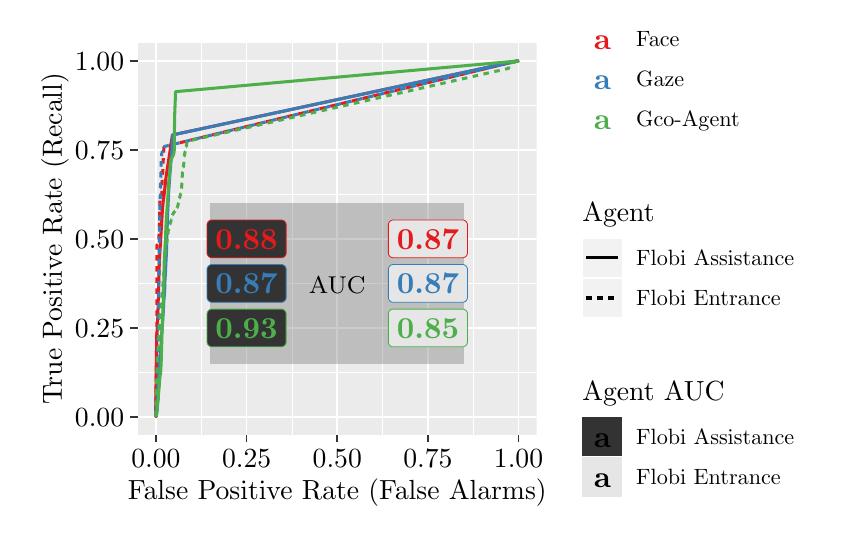
\begin{tikzpicture}[x=1pt,y=1pt]
\definecolor{fillColor}{RGB}{255,255,255}
\path[use as bounding box,fill=fillColor,fill opacity=0.00] (0,0) rectangle (288.00,177.98);
\begin{scope}
\path[clip] (  0.00,  0.00) rectangle (288.00,177.98);
\definecolor{drawColor}{RGB}{255,255,255}
\definecolor{fillColor}{RGB}{255,255,255}

\path[draw=drawColor,line width= 0.6pt,line join=round,line cap=round,fill=fillColor] (  0.00,  0.00) rectangle (288.00,177.98);
\end{scope}
\begin{scope}
\path[clip] ( 39.80, 30.86) rectangle (183.93,172.48);
\definecolor{fillColor}{gray}{0.92}

\path[fill=fillColor] ( 39.80, 30.86) rectangle (183.93,172.48);
\definecolor{drawColor}{RGB}{255,255,255}

\path[draw=drawColor,line width= 0.3pt,line join=round] ( 39.80, 53.38) --
	(183.93, 53.38);

\path[draw=drawColor,line width= 0.3pt,line join=round] ( 39.80, 85.57) --
	(183.93, 85.57);

\path[draw=drawColor,line width= 0.3pt,line join=round] ( 39.80,117.76) --
	(183.93,117.76);

\path[draw=drawColor,line width= 0.3pt,line join=round] ( 39.80,149.95) --
	(183.93,149.95);

\path[draw=drawColor,line width= 0.3pt,line join=round] ( 62.73, 30.86) --
	( 62.73,172.48);

\path[draw=drawColor,line width= 0.3pt,line join=round] ( 95.49, 30.86) --
	( 95.49,172.48);

\path[draw=drawColor,line width= 0.3pt,line join=round] (128.24, 30.86) --
	(128.24,172.48);

\path[draw=drawColor,line width= 0.3pt,line join=round] (161.00, 30.86) --
	(161.00,172.48);

\path[draw=drawColor,line width= 0.6pt,line join=round] ( 39.80, 37.28) --
	(183.93, 37.28);

\path[draw=drawColor,line width= 0.6pt,line join=round] ( 39.80, 69.47) --
	(183.93, 69.47);

\path[draw=drawColor,line width= 0.6pt,line join=round] ( 39.80,101.66) --
	(183.93,101.66);

\path[draw=drawColor,line width= 0.6pt,line join=round] ( 39.80,133.85) --
	(183.93,133.85);

\path[draw=drawColor,line width= 0.6pt,line join=round] ( 39.80,166.05) --
	(183.93,166.05);

\path[draw=drawColor,line width= 0.6pt,line join=round] ( 46.36, 30.86) --
	( 46.36,172.48);

\path[draw=drawColor,line width= 0.6pt,line join=round] ( 79.11, 30.86) --
	( 79.11,172.48);

\path[draw=drawColor,line width= 0.6pt,line join=round] (111.87, 30.86) --
	(111.87,172.48);

\path[draw=drawColor,line width= 0.6pt,line join=round] (144.62, 30.86) --
	(144.62,172.48);

\path[draw=drawColor,line width= 0.6pt,line join=round] (177.38, 30.86) --
	(177.38,172.48);
\definecolor{fillColor}{RGB}{89,89,89}

\path[fill=fillColor,fill opacity=0.30] ( 66.01, 56.60) rectangle (157.72,114.54);
\definecolor{drawColor}{RGB}{0,0,0}

\node[text=drawColor,anchor=base,inner sep=0pt, outer sep=0pt, scale=  1.10] at (111.87, 81.77) {\footnotesize{AUC}};
\definecolor{drawColor}{RGB}{228,26,28}

\path[draw=drawColor,line width= 1.1pt,line join=round] ( 46.36, 41.55) --
	( 46.36, 40.28) --
	( 46.36, 40.24) --
	( 46.36, 37.47) --
	( 46.38, 50.48) --
	( 46.38, 50.47) --
	( 46.38, 50.47) --
	( 46.39, 51.53) --
	( 46.52, 58.79) --
	( 46.63, 66.90) --
	( 46.63, 66.88) --
	( 46.63, 66.87) --
	( 46.63, 66.86) --
	( 46.94, 70.61) --
	( 47.28, 83.28) --
	( 47.59, 93.67) --
	( 47.60, 93.95) --
	( 47.61, 94.05) --
	( 48.02,100.77) --
	( 48.73,112.74) --
	( 49.08,116.24) --
	( 49.11,116.30) --
	( 49.17,116.44) --
	( 49.41,118.38) --
	( 49.90,123.25) --
	( 50.35,126.30) --
	( 50.39,126.47) --
	( 52.32,139.22) --
	(177.38,166.05);

\path[draw=drawColor,line width= 1.1pt,dash pattern=on 2pt off 2pt ,line join=round] ( 46.36, 38.92) --
	( 46.36, 37.89) --
	( 46.36, 37.69) --
	( 46.36, 37.42) --
	( 46.36, 44.37) --
	( 46.36, 44.35) --
	( 46.36, 44.30) --
	( 46.36, 43.42) --
	( 46.36, 42.24) --
	( 46.36, 39.58) --
	( 46.36, 45.75) --
	( 46.39, 45.75) --
	( 46.47, 54.57) --
	( 46.57, 56.12) --
	( 46.57, 55.86) --
	( 46.72, 61.90) --
	( 46.73, 99.42) --
	( 46.88, 99.72) --
	( 47.15,100.12) --
	( 47.26,100.15) --
	( 47.34,100.15) --
	( 47.38,101.19) --
	( 47.65,107.31) --
	( 47.83,116.26) --
	( 47.84,116.26) --
	( 47.88,116.26) --
	( 48.32,116.26) --
	( 48.35,116.28) --
	( 48.38,116.95) --
	( 48.46,118.02) --
	( 48.48,120.43) --
	( 48.50,120.43) --
	( 48.54,121.72) --
	( 48.57,123.47) --
	( 48.61,123.63) --
	( 48.67,123.63) --
	( 48.72,123.63) --
	( 48.79,125.42) --
	( 49.07,132.36) --
	( 49.27,134.98) --
	( 49.30,135.02) --
	(177.38,166.05);
\definecolor{drawColor}{RGB}{55,126,184}

\path[draw=drawColor,line width= 1.1pt,line join=round] ( 46.36, 37.30) --
	( 46.36, 37.31) --
	( 46.36, 37.34) --
	( 46.36, 37.35) --
	( 46.36, 37.37) --
	( 46.36, 37.39) --
	( 46.37, 37.41) --
	( 46.37, 37.43) --
	( 46.37, 37.44) --
	( 46.38, 37.46) --
	( 46.38, 37.48) --
	( 46.38, 37.52) --
	( 46.38, 37.54) --
	( 46.38, 37.56) --
	( 46.38, 37.59) --
	( 46.38, 37.61) --
	( 46.38, 37.63) --
	( 46.38, 37.65) --
	( 46.38, 37.67) --
	( 46.38, 37.69) --
	( 46.38, 37.71) --
	( 46.38, 37.73) --
	( 46.38, 37.75) --
	( 46.38, 37.77) --
	( 46.38, 37.78) --
	( 46.38, 37.80) --
	( 46.38, 37.82) --
	( 46.38, 37.85) --
	( 46.39, 37.86) --
	( 46.39, 37.88) --
	( 46.39, 37.90) --
	( 46.39, 37.92) --
	( 46.40, 37.93) --
	( 46.40, 37.96) --
	( 46.40, 37.98) --
	( 46.40, 37.99) --
	( 46.40, 38.01) --
	( 46.40, 38.03) --
	( 46.40, 38.05) --
	( 46.40, 38.08) --
	( 46.40, 38.10) --
	( 46.40, 38.12) --
	( 46.40, 38.13) --
	( 46.40, 38.16) --
	( 46.40, 38.18) --
	( 46.40, 38.21) --
	( 46.40, 38.23) --
	( 46.40, 38.25) --
	( 46.40, 38.28) --
	( 46.40, 38.30) --
	( 46.40, 38.32) --
	( 46.41, 38.33) --
	( 46.41, 38.35) --
	( 46.41, 38.37) --
	( 46.41, 38.38) --
	( 46.41, 38.41) --
	( 46.41, 38.43) --
	( 46.42, 38.45) --
	( 46.42, 38.48) --
	( 46.42, 38.50) --
	( 46.42, 38.52) --
	( 46.42, 38.54) --
	( 46.43, 38.56) --
	( 46.43, 38.58) --
	( 46.43, 38.61) --
	( 46.43, 38.63) --
	( 46.43, 38.65) --
	( 46.43, 38.68) --
	( 46.43, 38.70) --
	( 46.43, 38.72) --
	( 46.43, 38.74) --
	( 46.43, 38.76) --
	( 46.43, 38.78) --
	( 46.43, 38.80) --
	( 46.43, 38.83) --
	( 46.43, 38.85) --
	( 46.44, 38.87) --
	( 46.44, 38.90) --
	( 46.44, 38.92) --
	( 46.44, 38.94) --
	( 46.44, 38.97) --
	( 46.44, 38.99) --
	( 46.44, 39.01) --
	( 46.44, 39.03) --
	( 46.44, 39.05) --
	( 46.44, 39.07) --
	( 46.45, 39.09) --
	( 46.45, 39.10) --
	( 46.45, 39.12) --
	( 46.45, 39.14) --
	( 46.46, 39.16) --
	( 46.46, 39.18) --
	( 46.46, 39.20) --
	( 46.46, 39.21) --
	( 46.46, 39.23) --
	( 46.46, 39.25) --
	( 46.46, 39.28) --
	( 46.46, 39.30) --
	( 46.46, 39.31) --
	( 46.47, 39.33) --
	( 46.47, 39.35) --
	( 46.47, 39.37) --
	( 46.47, 39.38) --
	( 46.48, 39.40) --
	( 46.48, 39.42) --
	( 46.48, 39.44) --
	( 46.48, 39.45) --
	( 46.48, 39.48) --
	( 46.48, 39.50) --
	( 46.48, 39.52) --
	( 46.49, 39.54) --
	( 46.49, 39.56) --
	( 46.49, 39.57) --
	( 46.49, 39.59) --
	( 46.49, 39.61) --
	( 46.49, 39.63) --
	( 46.49, 39.65) --
	( 46.49, 39.67) --
	( 46.50, 39.69) --
	( 46.50, 39.71) --
	( 46.50, 39.73) --
	( 46.50, 39.75) --
	( 46.50, 39.76) --
	( 46.50, 39.78) --
	( 46.50, 39.80) --
	( 46.50, 39.82) --
	( 46.50, 39.84) --
	( 46.51, 39.86) --
	( 46.51, 39.88) --
	( 46.51, 39.91) --
	( 46.51, 39.95) --
	( 46.51, 39.97) --
	( 46.51, 39.99) --
	( 46.51, 40.01) --
	( 46.51, 40.03) --
	( 46.51, 40.06) --
	( 46.52, 40.07) --
	( 46.52, 40.09) --
	( 46.52, 40.11) --
	( 46.52, 40.13) --
	( 46.52, 40.16) --
	( 46.52, 40.18) --
	( 46.52, 40.20) --
	( 46.52, 40.22) --
	( 46.52, 40.25) --
	( 46.52, 40.27) --
	( 46.52, 40.29) --
	( 46.52, 40.32) --
	( 46.52, 40.34) --
	( 46.52, 40.36) --
	( 46.52, 40.38) --
	( 46.52, 40.40) --
	( 46.52, 40.42) --
	( 46.52, 40.44) --
	( 46.52, 40.45) --
	( 46.52, 40.47) --
	( 46.52, 40.49) --
	( 46.52, 40.51) --
	( 46.52, 40.54) --
	( 46.53, 40.55) --
	( 46.53, 40.57) --
	( 46.53, 40.59) --
	( 46.53, 40.60) --
	( 46.53, 40.63) --
	( 46.53, 40.65) --
	( 46.53, 40.68) --
	( 46.54, 40.69) --
	( 46.54, 40.71) --
	( 46.54, 40.73) --
	( 46.54, 40.75) --
	( 46.54, 40.77) --
	( 46.54, 40.79) --
	( 46.54, 40.81) --
	( 46.54, 40.83) --
	( 46.54, 40.85) --
	( 46.54, 40.87) --
	( 46.54, 40.89) --
	( 46.54, 40.91) --
	( 46.55, 40.92) --
	( 46.55, 40.94) --
	( 46.55, 40.96) --
	( 46.55, 40.98) --
	( 46.55, 41.00) --
	( 46.55, 41.03) --
	( 46.55, 41.05) --
	( 46.55, 41.07) --
	( 46.55, 41.09) --
	( 46.55, 41.11) --
	( 46.55, 41.15) --
	( 46.55, 41.17) --
	( 46.55, 41.19) --
	( 46.55, 41.21) --
	( 46.55, 41.23) --
	( 46.55, 41.25) --
	( 46.55, 41.27) --
	( 46.55, 41.29) --
	( 46.55, 41.31) --
	( 46.55, 41.33) --
	( 46.55, 41.35) --
	( 46.55, 41.37) --
	( 46.55, 41.39) --
	( 46.56, 41.40) --
	( 46.56, 41.42) --
	( 46.57, 41.43) --
	( 46.57, 41.44) --
	( 46.57, 41.46) --
	( 46.57, 41.48) --
	( 46.57, 41.50) --
	( 46.57, 41.52) --
	( 46.58, 41.53) --
	( 46.58, 41.57) --
	( 46.58, 41.59) --
	( 46.58, 41.61) --
	( 46.58, 41.63) --
	( 46.58, 41.65) --
	( 46.58, 41.67) --
	( 46.58, 41.69) --
	( 46.58, 41.71) --
	( 46.58, 41.73) --
	( 46.58, 41.75) --
	( 46.58, 41.76) --
	( 46.58, 41.78) --
	( 46.58, 41.80) --
	( 46.58, 41.82) --
	( 46.58, 41.85) --
	( 46.59, 41.86) --
	( 46.59, 41.88) --
	( 46.59, 41.90) --
	( 46.59, 41.92) --
	( 46.59, 41.94) --
	( 46.59, 41.95) --
	( 46.59, 41.97) --
	( 46.60, 41.99) --
	( 46.60, 42.01) --
	( 46.60, 42.03) --
	( 46.60, 42.05) --
	( 46.60, 42.07) --
	( 46.60, 42.09) --
	( 46.60, 42.11) --
	( 46.60, 42.13) --
	( 46.61, 42.14) --
	( 46.61, 42.16) --
	( 46.61, 42.18) --
	( 46.61, 42.20) --
	( 46.61, 42.23) --
	( 46.61, 42.25) --
	( 46.62, 42.26) --
	( 46.62, 42.28) --
	( 46.62, 42.31) --
	( 46.62, 42.34) --
	( 46.62, 42.35) --
	( 46.62, 42.37) --
	( 46.62, 42.39) --
	( 46.62, 42.41) --
	( 46.62, 42.43) --
	( 46.63, 42.45) --
	( 46.63, 42.47) --
	( 46.63, 42.48) --
	( 46.63, 42.50) --
	( 46.64, 42.52) --
	( 46.64, 42.55) --
	( 46.64, 42.56) --
	( 46.64, 42.59) --
	( 46.64, 42.62) --
	( 46.64, 42.63) --
	( 46.64, 42.65) --
	( 46.64, 42.67) --
	( 46.64, 42.69) --
	( 46.65, 42.71) --
	( 46.65, 42.73) --
	( 46.65, 42.74) --
	( 46.65, 42.77) --
	( 46.65, 42.79) --
	( 46.65, 42.82) --
	( 46.65, 42.84) --
	( 46.65, 42.86) --
	( 46.65, 42.89) --
	( 46.65, 42.91) --
	( 46.65, 42.93) --
	( 46.65, 42.95) --
	( 46.66, 42.96) --
	( 46.66, 42.98) --
	( 46.66, 43.00) --
	( 46.66, 43.02) --
	( 46.66, 43.04) --
	( 46.66, 43.07) --
	( 46.67, 43.08) --
	( 46.67, 43.10) --
	( 46.67, 43.12) --
	( 46.67, 43.14) --
	( 46.67, 43.15) --
	( 46.67, 43.17) --
	( 46.67, 43.19) --
	( 46.68, 43.20) --
	( 46.68, 43.21) --
	( 46.68, 43.23) --
	( 46.68, 43.25) --
	( 46.68, 43.27) --
	( 46.69, 43.29) --
	( 46.69, 43.32) --
	( 46.69, 43.34) --
	( 46.69, 43.36) --
	( 46.70, 43.38) --
	( 46.70, 43.40) --
	( 46.70, 43.43) --
	( 46.70, 43.45) --
	( 46.70, 43.48) --
	( 46.70, 43.50) --
	( 46.70, 43.52) --
	( 46.70, 43.54) --
	( 46.70, 43.55) --
	( 46.70, 43.57) --
	( 46.70, 43.59) --
	( 46.71, 43.60) --
	( 46.71, 43.61) --
	( 46.71, 43.63) --
	( 46.71, 43.65) --
	( 46.71, 43.67) --
	( 46.71, 43.70) --
	( 46.72, 43.71) --
	( 46.72, 43.74) --
	( 46.72, 43.76) --
	( 46.72, 43.79) --
	( 46.72, 43.81) --
	( 46.72, 43.83) --
	( 46.72, 43.85) --
	( 46.72, 43.86) --
	( 46.72, 43.88) --
	( 46.72, 43.90) --
	( 46.72, 43.93) --
	( 46.72, 43.95) --
	( 46.73, 43.97) --
	( 46.73, 43.99) --
	( 46.73, 44.01) --
	( 46.73, 44.03) --
	( 46.73, 44.05) --
	( 46.73, 44.07) --
	( 46.73, 44.09) --
	( 46.73, 44.11) --
	( 46.73, 44.13) --
	( 46.74, 44.15) --
	( 46.74, 44.17) --
	( 46.74, 44.20) --
	( 46.75, 44.22) --
	( 46.75, 44.23) --
	( 46.75, 44.25) --
	( 46.75, 44.27) --
	( 46.75, 44.30) --
	( 46.76, 44.32) --
	( 46.76, 44.34) --
	( 46.76, 44.35) --
	( 46.76, 44.37) --
	( 46.76, 44.39) --
	( 46.77, 44.40) --
	( 46.78, 44.41) --
	( 46.78, 44.43) --
	( 46.78, 44.44) --
	( 46.78, 44.47) --
	( 46.78, 44.50) --
	( 46.79, 44.52) --
	( 46.79, 44.54) --
	( 46.79, 44.56) --
	( 46.79, 44.58) --
	( 46.79, 44.59) --
	( 46.79, 44.61) --
	( 46.79, 44.64) --
	( 46.79, 44.66) --
	( 46.79, 44.68) --
	( 46.79, 44.71) --
	( 46.79, 44.73) --
	( 46.79, 44.75) --
	( 46.79, 44.77) --
	( 46.79, 44.80) --
	( 46.80, 44.82) --
	( 46.81, 44.83) --
	( 46.81, 44.85) --
	( 46.81, 44.87) --
	( 46.81, 44.89) --
	( 46.81, 44.91) --
	( 46.81, 44.92) --
	( 46.82, 44.94) --
	( 46.82, 44.96) --
	( 46.82, 44.97) --
	( 46.82, 44.99) --
	( 46.82, 45.02) --
	( 46.83, 45.03) --
	( 46.83, 45.05) --
	( 46.83, 45.08) --
	( 46.83, 45.10) --
	( 46.83, 45.11) --
	( 46.83, 45.13) --
	( 46.83, 45.15) --
	( 46.83, 45.17) --
	( 46.83, 45.19) --
	( 46.83, 45.21) --
	( 46.83, 45.23) --
	( 46.83, 45.25) --
	( 46.83, 45.27) --
	( 46.83, 45.29) --
	( 46.83, 45.31) --
	( 46.83, 45.33) --
	( 46.83, 45.34) --
	( 46.83, 45.36) --
	( 46.84, 45.38) --
	( 46.84, 45.40) --
	( 46.84, 45.42) --
	( 46.84, 45.44) --
	( 46.84, 45.46) --
	( 46.85, 45.47) --
	( 46.85, 45.49) --
	( 46.86, 45.51) --
	( 46.86, 45.55) --
	( 46.86, 45.57) --
	( 46.86, 45.60) --
	( 46.86, 45.62) --
	( 46.86, 45.64) --
	( 46.86, 45.67) --
	( 46.86, 45.69) --
	( 46.86, 45.71) --
	( 46.86, 45.73) --
	( 46.86, 45.75) --
	( 46.86, 45.77) --
	( 46.86, 45.79) --
	( 46.86, 45.81) --
	( 46.86, 45.82) --
	( 46.87, 45.84) --
	( 46.87, 45.86) --
	( 46.87, 45.88) --
	( 46.88, 45.90) --
	( 46.88, 45.91) --
	( 46.88, 45.93) --
	( 46.89, 45.94) --
	( 46.89, 45.97) --
	( 46.89, 45.99) --
	( 46.89, 46.01) --
	( 46.89, 46.02) --
	( 46.89, 46.04) --
	( 46.90, 46.05) --
	( 46.90, 46.07) --
	( 46.90, 46.09) --
	( 46.90, 46.11) --
	( 46.90, 46.14) --
	( 46.90, 46.16) --
	( 46.90, 46.18) --
	( 46.90, 46.20) --
	( 46.90, 46.22) --
	( 46.90, 46.24) --
	( 46.91, 46.25) --
	( 46.91, 46.27) --
	( 46.91, 46.29) --
	( 46.91, 46.31) --
	( 46.91, 46.33) --
	( 46.91, 46.35) --
	( 46.91, 46.37) --
	( 46.91, 46.39) --
	( 46.91, 46.41) --
	( 46.91, 46.43) --
	( 46.91, 46.46) --
	( 46.91, 46.47) --
	( 46.92, 46.49) --
	( 46.92, 46.51) --
	( 46.92, 46.53) --
	( 46.92, 46.55) --
	( 46.92, 46.56) --
	( 46.92, 46.58) --
	( 46.94, 46.59) --
	( 46.94, 46.61) --
	( 46.94, 46.63) --
	( 46.94, 46.66) --
	( 46.94, 46.68) --
	( 46.94, 46.70) --
	( 46.94, 46.72) --
	( 46.94, 46.73) --
	( 46.94, 46.75) --
	( 46.94, 46.77) --
	( 46.94, 46.81) --
	( 46.94, 46.83) --
	( 46.94, 46.85) --
	( 46.95, 46.86) --
	( 46.95, 46.88) --
	( 46.95, 46.91) --
	( 46.96, 46.92) --
	( 46.96, 46.94) --
	( 46.96, 46.96) --
	( 46.97, 46.97) --
	( 46.97, 46.98) --
	( 46.97, 47.00) --
	( 46.97, 47.03) --
	( 46.98, 47.04) --
	( 46.98, 47.07) --
	( 46.98, 47.09) --
	( 46.98, 47.11) --
	( 46.98, 47.13) --
	( 46.98, 47.15) --
	( 46.98, 47.17) --
	( 46.98, 47.19) --
	( 46.99, 47.20) --
	( 46.99, 47.23) --
	( 46.99, 47.25) --
	( 46.99, 47.27) --
	( 46.99, 47.29) --
	( 46.99, 47.31) --
	( 46.99, 47.32) --
	( 46.99, 47.34) --
	( 46.99, 47.36) --
	( 46.99, 47.39) --
	( 46.99, 47.41) --
	( 46.99, 47.43) --
	( 46.99, 47.44) --
	( 46.99, 47.46) --
	( 46.99, 47.48) --
	( 47.00, 47.50) --
	( 47.00, 47.51) --
	( 47.00, 47.53) --
	( 47.01, 47.54) --
	( 47.01, 47.56) --
	( 47.01, 47.57) --
	( 47.01, 47.59) --
	( 47.01, 47.61) --
	( 47.01, 47.65) --
	( 47.01, 47.67) --
	( 47.02, 47.68) --
	( 47.02, 47.70) --
	( 47.02, 47.71) --
	( 47.03, 47.72) --
	( 47.03, 47.74) --
	( 47.03, 47.76) --
	( 47.03, 47.78) --
	( 47.03, 47.80) --
	( 47.03, 47.82) --
	( 47.04, 47.83) --
	( 47.04, 47.85) --
	( 47.04, 47.87) --
	( 47.04, 47.89) --
	( 47.04, 47.90) --
	( 47.04, 47.92) --
	( 47.04, 47.94) --
	( 47.04, 47.96) --
	( 47.04, 47.99) --
	( 47.04, 48.01) --
	( 47.04, 48.02) --
	( 47.04, 48.04) --
	( 47.04, 48.07) --
	( 47.05, 48.08) --
	( 47.05, 48.11) --
	( 47.05, 48.13) --
	( 47.05, 48.16) --
	( 47.05, 48.18) --
	( 47.05, 48.20) --
	( 47.05, 48.22) --
	( 47.05, 48.24) --
	( 47.05, 48.26) --
	( 47.06, 48.28) --
	( 47.06, 48.30) --
	( 47.06, 48.32) --
	( 47.06, 48.34) --
	( 47.06, 48.35) --
	( 47.06, 48.37) --
	( 47.07, 48.39) --
	( 47.07, 48.41) --
	( 47.07, 48.43) --
	( 47.07, 48.45) --
	( 47.07, 48.47) --
	( 47.07, 48.48) --
	( 47.07, 48.50) --
	( 47.07, 48.52) --
	( 47.07, 48.54) --
	( 47.08, 48.56) --
	( 47.08, 48.58) --
	( 47.09, 48.58) --
	( 47.09, 48.60) --
	( 47.09, 48.62) --
	( 47.09, 48.64) --
	( 47.09, 48.66) --
	( 47.09, 48.68) --
	( 47.09, 48.70) --
	( 47.09, 48.72) --
	( 47.09, 48.73) --
	( 47.09, 48.76) --
	( 47.09, 48.78) --
	( 47.10, 48.79) --
	( 47.10, 48.81) --
	( 47.10, 48.83) --
	( 47.10, 48.85) --
	( 47.11, 48.86) --
	( 47.11, 48.87) --
	( 47.11, 48.91) --
	( 47.11, 48.92) --
	( 47.11, 48.94) --
	( 47.12, 48.96) --
	( 47.12, 48.98) --
	( 47.12, 49.00) --
	( 47.12, 49.03) --
	( 47.12, 49.06) --
	( 47.13, 49.06) --
	( 47.13, 49.08) --
	( 47.13, 49.10) --
	( 47.13, 49.13) --
	( 47.13, 49.15) --
	( 47.13, 49.17) --
	( 47.13, 49.19) --
	( 47.13, 49.21) --
	( 47.14, 49.23) --
	( 47.14, 49.25) --
	( 47.14, 49.27) --
	( 47.14, 49.29) --
	( 47.14, 49.30) --
	( 47.14, 49.32) --
	( 47.14, 49.34) --
	( 47.14, 49.37) --
	( 47.15, 49.38) --
	( 47.15, 49.41) --
	( 47.15, 49.43) --
	( 47.15, 49.45) --
	( 47.15, 49.47) --
	( 47.15, 49.49) --
	( 47.15, 49.50) --
	( 47.16, 49.51) --
	( 47.16, 49.54) --
	( 47.16, 49.56) --
	( 47.16, 49.59) --
	( 47.17, 49.60) --
	( 47.17, 49.61) --
	( 47.17, 49.63) --
	( 47.17, 49.65) --
	( 47.17, 49.67) --
	( 47.17, 49.70) --
	( 47.17, 49.71) --
	( 47.17, 49.74) --
	( 47.17, 49.76) --
	( 47.17, 49.78) --
	( 47.17, 49.80) --
	( 47.17, 49.82) --
	( 47.17, 49.85) --
	( 47.17, 49.87) --
	( 47.17, 49.89) --
	( 47.17, 49.91) --
	( 47.18, 49.91) --
	( 47.18, 49.94) --
	( 47.19, 49.95) --
	( 47.20, 49.96) --
	( 47.20, 49.98) --
	( 47.20, 50.01) --
	( 47.20, 50.03) --
	( 47.20, 50.05) --
	( 47.20, 50.07) --
	( 47.20, 50.08) --
	( 47.20, 50.11) --
	( 47.20, 50.12) --
	( 47.21, 50.14) --
	( 47.21, 50.16) --
	( 47.21, 50.18) --
	( 47.21, 50.20) --
	( 47.21, 50.22) --
	( 47.21, 50.25) --
	( 47.21, 50.27) --
	( 47.21, 50.29) --
	( 47.21, 50.31) --
	( 47.22, 50.33) --
	( 47.22, 50.35) --
	( 47.22, 50.37) --
	( 47.22, 50.39) --
	( 47.22, 50.41) --
	( 47.22, 50.43) --
	( 47.22, 50.45) --
	( 47.22, 50.47) --
	( 47.22, 50.49) --
	( 47.22, 50.51) --
	( 47.23, 50.52) --
	( 47.23, 50.54) --
	( 47.23, 50.56) --
	( 47.23, 50.57) --
	( 47.24, 50.58) --
	( 47.24, 50.60) --
	( 47.24, 50.62) --
	( 47.24, 50.64) --
	( 47.24, 50.66) --
	( 47.24, 50.68) --
	( 47.25, 50.69) --
	( 47.25, 50.71) --
	( 47.25, 50.73) --
	( 47.25, 50.75) --
	( 47.25, 50.76) --
	( 47.25, 50.78) --
	( 47.25, 50.80) --
	( 47.25, 50.83) --
	( 47.25, 50.85) --
	( 47.26, 50.87) --
	( 47.26, 50.89) --
	( 47.26, 50.90) --
	( 47.26, 50.92) --
	( 47.26, 50.94) --
	( 47.27, 50.96) --
	( 47.27, 50.98) --
	( 47.27, 51.00) --
	( 47.27, 51.02) --
	( 47.27, 51.04) --
	( 47.27, 51.07) --
	( 47.27, 51.09) --
	( 47.27, 51.11) --
	( 47.27, 51.13) --
	( 47.27, 51.14) --
	( 47.27, 51.16) --
	( 47.27, 51.18) --
	( 47.27, 51.20) --
	( 47.27, 51.23) --
	( 47.28, 51.24) --
	( 47.28, 51.25) --
	( 47.28, 51.28) --
	( 47.28, 51.30) --
	( 47.28, 51.32) --
	( 47.28, 51.34) --
	( 47.28, 51.38) --
	( 47.29, 51.40) --
	( 47.29, 51.42) --
	( 47.29, 51.44) --
	( 47.29, 51.46) --
	( 47.29, 51.48) --
	( 47.29, 51.49) --
	( 47.29, 51.53) --
	( 47.29, 51.55) --
	( 47.29, 51.57) --
	( 47.29, 51.60) --
	( 47.29, 51.61) --
	( 47.31, 51.61) --
	( 47.31, 51.63) --
	( 47.31, 51.65) --
	( 47.31, 51.67) --
	( 47.31, 51.69) --
	( 47.31, 51.70) --
	( 47.32, 51.72) --
	( 47.33, 51.74) --
	( 47.33, 51.76) --
	( 47.33, 51.78) --
	( 47.33, 51.82) --
	( 47.33, 51.83) --
	( 47.33, 51.86) --
	( 47.33, 51.88) --
	( 47.33, 51.89) --
	( 47.33, 51.91) --
	( 47.33, 51.93) --
	( 47.34, 51.95) --
	( 47.34, 51.97) --
	( 47.34, 51.99) --
	( 47.34, 52.01) --
	( 47.35, 52.03) --
	( 47.35, 52.05) --
	( 47.35, 52.06) --
	( 47.35, 52.09) --
	( 47.36, 52.10) --
	( 47.36, 52.12) --
	( 47.36, 52.14) --
	( 47.36, 52.16) --
	( 47.36, 52.19) --
	( 47.36, 52.21) --
	( 47.36, 52.23) --
	( 47.36, 52.25) --
	( 47.36, 52.26) --
	( 47.36, 52.28) --
	( 47.37, 52.29) --
	( 47.37, 52.31) --
	( 47.37, 52.33) --
	( 47.37, 52.35) --
	( 47.37, 52.39) --
	( 47.37, 52.41) --
	( 47.37, 52.43) --
	( 47.38, 52.43) --
	( 47.38, 52.45) --
	( 47.38, 52.47) --
	( 47.38, 52.50) --
	( 47.38, 52.52) --
	( 47.38, 52.54) --
	( 47.38, 52.56) --
	( 47.39, 52.57) --
	( 47.40, 52.59) --
	( 47.40, 52.62) --
	( 47.40, 52.64) --
	( 47.40, 52.66) --
	( 47.40, 52.68) --
	( 47.40, 52.69) --
	( 47.40, 52.72) --
	( 47.40, 52.75) --
	( 47.40, 52.77) --
	( 47.40, 52.79) --
	( 47.41, 52.81) --
	( 47.41, 52.83) --
	( 47.41, 52.84) --
	( 47.41, 52.86) --
	( 47.42, 52.88) --
	( 47.42, 52.90) --
	( 47.42, 52.91) --
	( 47.42, 52.94) --
	( 47.42, 52.96) --
	( 47.42, 52.98) --
	( 47.43, 53.00) --
	( 47.43, 53.02) --
	( 47.43, 53.04) --
	( 47.44, 53.04) --
	( 47.44, 53.06) --
	( 47.44, 53.09) --
	( 47.44, 53.11) --
	( 47.44, 53.13) --
	( 47.44, 53.16) --
	( 47.45, 53.17) --
	( 47.46, 53.18) --
	( 47.46, 53.21) --
	( 47.46, 53.23) --
	( 47.46, 53.25) --
	( 47.46, 53.29) --
	( 47.46, 53.30) --
	( 47.47, 53.32) --
	( 47.47, 53.34) --
	( 47.47, 53.35) --
	( 47.47, 53.37) --
	( 47.47, 53.39) --
	( 47.47, 53.41) --
	( 47.48, 53.42) --
	( 47.48, 53.44) --
	( 47.48, 53.46) --
	( 47.48, 53.49) --
	( 47.48, 53.51) --
	( 47.48, 53.53) --
	( 47.49, 53.55) --
	( 47.49, 53.56) --
	( 47.49, 53.59) --
	( 47.50, 53.60) --
	( 47.50, 53.62) --
	( 47.50, 53.65) --
	( 47.50, 53.67) --
	( 47.50, 53.69) --
	( 47.50, 53.70) --
	( 47.51, 53.72) --
	( 47.51, 53.74) --
	( 47.51, 53.76) --
	( 47.51, 53.79) --
	( 47.51, 53.82) --
	( 47.51, 53.84) --
	( 47.51, 53.86) --
	( 47.51, 53.87) --
	( 47.51, 53.90) --
	( 47.51, 53.92) --
	( 47.51, 53.95) --
	( 47.51, 53.97) --
	( 47.51, 53.99) --
	( 47.51, 54.01) --
	( 47.51, 54.03) --
	( 47.51, 54.05) --
	( 47.52, 54.07) --
	( 47.52, 54.08) --
	( 47.52, 54.12) --
	( 47.52, 54.14) --
	( 47.52, 54.16) --
	( 47.52, 54.19) --
	( 47.53, 54.20) --
	( 47.53, 54.22) --
	( 47.53, 54.24) --
	( 47.53, 54.26) --
	( 47.53, 54.28) --
	( 47.53, 54.30) --
	( 47.54, 54.31) --
	( 47.54, 54.33) --
	( 47.54, 54.36) --
	( 47.54, 54.38) --
	( 47.54, 54.39) --
	( 47.55, 54.41) --
	( 47.55, 54.42) --
	( 47.56, 54.43) --
	( 47.56, 54.45) --
	( 47.56, 54.47) --
	( 47.57, 54.48) --
	( 47.57, 54.51) --
	( 47.57, 54.53) --
	( 47.57, 54.54) --
	( 47.57, 54.58) --
	( 47.57, 54.60) --
	( 47.57, 54.62) --
	( 47.57, 54.64) --
	( 47.57, 54.66) --
	( 47.57, 54.68) --
	( 47.57, 54.71) --
	( 47.57, 54.73) --
	( 47.57, 54.75) --
	( 47.57, 54.77) --
	( 47.57, 54.79) --
	( 47.58, 54.81) --
	( 47.58, 54.83) --
	( 47.58, 54.85) --
	( 47.58, 54.87) --
	( 47.58, 54.89) --
	( 47.58, 54.91) --
	( 47.58, 54.93) --
	( 47.58, 54.95) --
	( 47.58, 54.98) --
	( 47.58, 55.00) --
	( 47.58, 55.03) --
	( 47.58, 55.05) --
	( 47.58, 55.07) --
	( 47.58, 55.09) --
	( 47.58, 55.11) --
	( 47.58, 55.13) --
	( 47.58, 55.17) --
	( 47.58, 55.19) --
	( 47.59, 55.20) --
	( 47.59, 55.22) --
	( 47.59, 55.24) --
	( 47.59, 55.26) --
	( 47.59, 55.28) --
	( 47.59, 55.30) --
	( 47.59, 55.32) --
	( 47.59, 55.34) --
	( 47.59, 55.36) --
	( 47.60, 55.38) --
	( 47.60, 55.40) --
	( 47.60, 55.41) --
	( 47.60, 55.43) --
	( 47.60, 55.45) --
	( 47.61, 55.46) --
	( 47.61, 55.49) --
	( 47.61, 55.51) --
	( 47.61, 55.53) --
	( 47.61, 55.55) --
	( 47.61, 55.57) --
	( 47.61, 55.60) --
	( 47.61, 55.62) --
	( 47.61, 55.65) --
	( 47.61, 55.67) --
	( 47.61, 55.70) --
	( 47.61, 55.72) --
	( 47.61, 55.74) --
	( 47.61, 55.76) --
	( 47.61, 55.78) --
	( 47.62, 55.79) --
	( 47.62, 55.81) --
	( 47.62, 55.82) --
	( 47.62, 55.85) --
	( 47.62, 55.87) --
	( 47.62, 55.89) --
	( 47.62, 55.92) --
	( 47.62, 55.94) --
	( 47.62, 55.97) --
	( 47.62, 56.00) --
	( 47.62, 56.02) --
	( 47.62, 56.04) --
	( 47.63, 56.05) --
	( 47.63, 56.08) --
	( 47.63, 56.10) --
	( 47.64, 56.11) --
	( 47.64, 56.13) --
	( 47.64, 56.15) --
	( 47.64, 56.17) --
	( 47.64, 56.20) --
	( 47.64, 56.22) --
	( 47.64, 56.24) --
	( 47.64, 56.26) --
	( 47.64, 56.28) --
	( 47.64, 56.30) --
	( 47.64, 56.32) --
	( 47.64, 56.35) --
	( 47.65, 56.36) --
	( 47.65, 56.37) --
	( 47.65, 56.40) --
	( 47.65, 56.42) --
	( 47.65, 56.45) --
	( 47.65, 56.47) --
	( 47.65, 56.50) --
	( 47.65, 56.52) --
	( 47.65, 56.54) --
	( 47.65, 56.56) --
	( 47.65, 56.58) --
	( 47.65, 56.60) --
	( 47.65, 56.62) --
	( 47.66, 56.64) --
	( 47.66, 56.66) --
	( 47.66, 56.67) --
	( 47.66, 56.69) --
	( 47.67, 56.71) --
	( 47.67, 56.73) --
	( 47.67, 56.75) --
	( 47.67, 56.77) --
	( 47.67, 56.79) --
	( 47.67, 56.81) --
	( 47.67, 56.83) --
	( 47.68, 56.85) --
	( 47.68, 56.86) --
	( 47.68, 56.89) --
	( 47.68, 56.90) --
	( 47.69, 56.92) --
	( 47.69, 56.94) --
	( 47.69, 56.96) --
	( 47.69, 56.98) --
	( 47.69, 57.00) --
	( 47.69, 57.02) --
	( 47.69, 57.04) --
	( 47.69, 57.05) --
	( 47.70, 57.07) --
	( 47.70, 57.09) --
	( 47.70, 57.10) --
	( 47.70, 57.12) --
	( 47.71, 57.13) --
	( 47.71, 57.15) --
	( 47.71, 57.17) --
	( 47.71, 57.19) --
	( 47.71, 57.21) --
	( 47.72, 57.23) --
	( 47.72, 57.25) --
	( 47.72, 57.27) --
	( 47.72, 57.30) --
	( 47.72, 57.34) --
	( 47.72, 57.36) --
	( 47.72, 57.38) --
	( 47.72, 57.40) --
	( 47.72, 57.42) --
	( 47.73, 57.42) --
	( 47.74, 57.44) --
	( 47.74, 57.45) --
	( 47.74, 57.47) --
	( 47.74, 57.49) --
	( 47.74, 57.51) --
	( 47.74, 57.54) --
	( 47.75, 57.55) --
	( 47.75, 57.57) --
	( 47.75, 57.59) --
	( 47.75, 57.61) --
	( 47.75, 57.63) --
	( 47.75, 57.64) --
	( 47.75, 57.66) --
	( 47.75, 57.68) --
	( 47.76, 57.70) --
	( 47.76, 57.73) --
	( 47.76, 57.76) --
	( 47.76, 57.78) --
	( 47.77, 57.79) --
	( 47.77, 57.81) --
	( 47.78, 57.82) --
	( 47.78, 57.84) --
	( 47.78, 57.87) --
	( 47.78, 57.89) --
	( 47.78, 57.91) --
	( 47.78, 57.93) --
	( 47.78, 57.96) --
	( 47.79, 57.97) --
	( 47.79, 58.00) --
	( 47.79, 58.02) --
	( 47.79, 58.05) --
	( 47.79, 58.07) --
	( 47.79, 58.09) --
	( 47.79, 58.11) --
	( 47.79, 58.12) --
	( 47.79, 58.15) --
	( 47.79, 58.17) --
	( 47.80, 58.18) --
	( 47.80, 58.20) --
	( 47.80, 58.22) --
	( 47.80, 58.24) --
	( 47.80, 58.26) --
	( 47.80, 58.28) --
	( 47.80, 58.30) --
	( 47.81, 58.31) --
	( 47.81, 58.33) --
	( 47.82, 58.35) --
	( 47.82, 58.37) --
	( 47.82, 58.40) --
	( 47.82, 58.43) --
	( 47.82, 58.44) --
	( 47.82, 58.46) --
	( 47.82, 58.48) --
	( 47.82, 58.51) --
	( 47.82, 58.53) --
	( 47.83, 58.54) --
	( 47.83, 58.57) --
	( 47.83, 58.59) --
	( 47.83, 58.61) --
	( 47.83, 58.63) --
	( 47.83, 58.66) --
	( 47.83, 58.67) --
	( 47.83, 58.69) --
	( 47.83, 58.71) --
	( 47.83, 58.73) --
	( 47.83, 58.75) --
	( 47.83, 58.77) --
	( 47.83, 58.79) --
	( 47.83, 58.81) --
	( 47.83, 58.84) --
	( 47.83, 58.86) --
	( 47.83, 58.88) --
	( 47.83, 58.90) --
	( 47.83, 58.92) --
	( 47.83, 58.95) --
	( 47.83, 58.97) --
	( 47.84, 58.99) --
	( 47.84, 59.01) --
	( 47.84, 59.03) --
	( 47.84, 59.05) --
	( 47.85, 59.06) --
	( 47.85, 59.08) --
	( 47.85, 59.11) --
	( 47.85, 59.13) --
	( 47.85, 59.15) --
	( 47.86, 59.17) --
	( 47.86, 59.19) --
	( 47.86, 59.21) --
	( 47.86, 59.23) --
	( 47.86, 59.24) --
	( 47.87, 59.26) --
	( 47.87, 59.28) --
	( 47.87, 59.30) --
	( 47.87, 59.32) --
	( 47.87, 59.34) --
	( 47.87, 59.36) --
	( 47.87, 59.38) --
	( 47.87, 59.41) --
	( 47.87, 59.43) --
	( 47.88, 59.44) --
	( 47.88, 59.45) --
	( 47.88, 59.48) --
	( 47.88, 59.51) --
	( 47.88, 59.53) --
	( 47.89, 59.54) --
	( 47.89, 59.57) --
	( 47.89, 59.59) --
	( 47.89, 59.61) --
	( 47.90, 59.63) --
	( 47.90, 59.64) --
	( 47.90, 59.67) --
	( 47.90, 59.69) --
	( 47.90, 59.71) --
	( 47.90, 59.73) --
	( 47.90, 59.77) --
	( 47.90, 59.80) --
	( 47.90, 59.82) --
	( 47.90, 59.84) --
	( 47.91, 59.85) --
	( 47.91, 59.87) --
	( 47.91, 59.89) --
	( 47.91, 59.90) --
	( 47.91, 59.93) --
	( 47.91, 59.95) --
	( 47.91, 59.97) --
	( 47.92, 59.99) --
	( 47.92, 60.01) --
	( 47.92, 60.03) --
	( 47.92, 60.06) --
	( 47.92, 60.08) --
	( 47.92, 60.11) --
	( 47.92, 60.12) --
	( 47.93, 60.14) --
	( 47.93, 60.16) --
	( 47.93, 60.17) --
	( 47.93, 60.18) --
	( 47.93, 60.20) --
	( 47.94, 60.22) --
	( 47.94, 60.23) --
	( 47.94, 60.25) --
	( 47.94, 60.27) --
	( 47.94, 60.29) --
	( 47.94, 60.31) --
	( 47.94, 60.33) --
	( 47.94, 60.35) --
	( 47.94, 60.37) --
	( 47.94, 60.40) --
	( 47.94, 60.43) --
	( 47.95, 60.45) --
	( 47.95, 60.47) --
	( 47.95, 60.50) --
	( 47.95, 60.52) --
	( 47.96, 60.54) --
	( 47.96, 60.55) --
	( 47.96, 60.58) --
	( 47.96, 60.60) --
	( 47.96, 60.63) --
	( 47.97, 60.64) --
	( 47.97, 60.67) --
	( 47.97, 60.69) --
	( 47.97, 60.71) --
	( 47.97, 60.73) --
	( 47.97, 60.74) --
	( 47.97, 60.76) --
	( 47.97, 60.78) --
	( 47.98, 60.79) --
	( 47.98, 60.81) --
	( 47.99, 60.82) --
	( 47.99, 60.84) --
	( 47.99, 60.86) --
	( 47.99, 60.88) --
	( 47.99, 60.90) --
	( 47.99, 60.92) --
	( 47.99, 60.94) --
	( 48.00, 60.96) --
	( 48.00, 60.98) --
	( 48.00, 61.00) --
	( 48.00, 61.02) --
	( 48.00, 61.04) --
	( 48.00, 61.06) --
	( 48.00, 61.08) --
	( 48.01, 61.09) --
	( 48.01, 61.11) --
	( 48.01, 61.13) --
	( 48.02, 61.13) --
	( 48.02, 61.15) --
	( 48.02, 61.17) --
	( 48.02, 61.19) --
	( 48.03, 61.20) --
	( 48.03, 61.22) --
	( 48.03, 61.24) --
	( 48.03, 61.27) --
	( 48.03, 61.30) --
	( 48.03, 61.32) --
	( 48.03, 61.34) --
	( 48.03, 61.36) --
	( 48.03, 61.38) --
	( 48.03, 61.40) --
	( 48.03, 61.42) --
	( 48.03, 61.44) --
	( 48.03, 61.46) --
	( 48.03, 61.48) --
	( 48.03, 61.51) --
	( 48.03, 61.55) --
	( 48.03, 61.57) --
	( 48.03, 61.60) --
	( 48.04, 61.61) --
	( 48.04, 61.63) --
	( 48.05, 61.64) --
	( 48.05, 61.66) --
	( 48.05, 61.69) --
	( 48.06, 61.70) --
	( 48.06, 61.72) --
	( 48.06, 61.74) --
	( 48.07, 61.75) --
	( 48.07, 61.77) --
	( 48.07, 61.79) --
	( 48.07, 61.81) --
	( 48.07, 61.83) --
	( 48.07, 61.85) --
	( 48.08, 61.85) --
	( 48.08, 61.87) --
	( 48.09, 61.89) --
	( 48.09, 61.90) --
	( 48.09, 61.93) --
	( 48.09, 61.95) --
	( 48.09, 61.97) --
	( 48.09, 61.99) --
	( 48.09, 62.02) --
	( 48.09, 62.04) --
	( 48.09, 62.06) --
	( 48.09, 62.08) --
	( 48.09, 62.10) --
	( 48.09, 62.12) --
	( 48.09, 62.14) --
	( 48.09, 62.16) --
	( 48.09, 62.18) --
	( 48.09, 62.21) --
	( 48.09, 62.23) --
	( 48.09, 62.25) --
	( 48.09, 62.27) --
	( 48.09, 62.29) --
	( 48.10, 62.31) --
	( 48.10, 62.32) --
	( 48.10, 62.34) --
	( 48.10, 62.36) --
	( 48.11, 62.37) --
	( 48.11, 62.39) --
	( 48.11, 62.41) --
	( 48.11, 62.44) --
	( 48.11, 62.46) --
	( 48.11, 62.48) --
	( 48.12, 62.49) --
	( 48.12, 62.51) --
	( 48.12, 62.53) --
	( 48.12, 62.56) --
	( 48.12, 62.58) --
	( 48.12, 62.60) --
	( 48.12, 62.62) --
	( 48.13, 62.63) --
	( 48.13, 62.66) --
	( 48.13, 62.67) --
	( 48.13, 62.69) --
	( 48.14, 62.70) --
	( 48.14, 62.72) --
	( 48.14, 62.75) --
	( 48.14, 62.77) --
	( 48.14, 62.78) --
	( 48.14, 62.81) --
	( 48.15, 62.82) --
	( 48.15, 62.84) --
	( 48.15, 62.87) --
	( 48.15, 62.89) --
	( 48.15, 62.91) --
	( 48.16, 62.92) --
	( 48.16, 62.94) --
	( 48.16, 62.96) --
	( 48.16, 62.98) --
	( 48.16, 63.00) --
	( 48.16, 63.02) --
	( 48.16, 63.03) --
	( 48.17, 63.05) --
	( 48.17, 63.07) --
	( 48.17, 63.09) --
	( 48.17, 63.11) --
	( 48.17, 63.13) --
	( 48.17, 63.15) --
	( 48.17, 63.17) --
	( 48.17, 63.19) --
	( 48.17, 63.21) --
	( 48.17, 63.23) --
	( 48.17, 63.26) --
	( 48.18, 63.27) --
	( 48.18, 63.28) --
	( 48.18, 63.31) --
	( 48.18, 63.33) --
	( 48.18, 63.35) --
	( 48.18, 63.37) --
	( 48.18, 63.39) --
	( 48.18, 63.41) --
	( 48.19, 63.43) --
	( 48.19, 63.45) --
	( 48.19, 63.47) --
	( 48.19, 63.49) --
	( 48.19, 63.53) --
	( 48.19, 63.56) --
	( 48.19, 63.58) --
	( 48.20, 63.59) --
	( 48.20, 63.61) --
	( 48.20, 63.62) --
	( 48.20, 63.65) --
	( 48.20, 63.67) --
	( 48.20, 63.69) --
	( 48.20, 63.72) --
	( 48.20, 63.73) --
	( 48.20, 63.76) --
	( 48.21, 63.77) --
	( 48.21, 63.80) --
	( 48.21, 63.82) --
	( 48.21, 63.84) --
	( 48.22, 63.85) --
	( 48.22, 63.87) --
	( 48.22, 63.89) --
	( 48.22, 63.91) --
	( 48.22, 63.93) --
	( 48.23, 63.95) --
	( 48.23, 63.97) --
	( 48.24, 63.98) --
	( 48.24, 63.99) --
	( 48.24, 64.02) --
	( 48.24, 64.04) --
	( 48.24, 64.06) --
	( 48.24, 64.08) --
	( 48.25, 64.10) --
	( 48.25, 64.12) --
	( 48.25, 64.14) --
	( 48.25, 64.16) --
	( 48.25, 64.18) --
	( 48.25, 64.20) --
	( 48.25, 64.23) --
	( 48.25, 64.25) --
	( 48.25, 64.27) --
	( 48.25, 64.30) --
	( 48.25, 64.33) --
	( 48.25, 64.35) --
	( 48.25, 64.36) --
	( 48.25, 64.38) --
	( 48.25, 64.41) --
	( 48.25, 64.42) --
	( 48.25, 64.44) --
	( 48.25, 64.47) --
	( 48.25, 64.48) --
	( 48.25, 64.51) --
	( 48.25, 64.53) --
	( 48.25, 64.55) --
	( 48.25, 64.57) --
	( 48.25, 64.60) --
	( 48.25, 64.61) --
	( 48.26, 64.63) --
	( 48.26, 64.65) --
	( 48.26, 64.67) --
	( 48.26, 64.69) --
	( 48.26, 64.71) --
	( 48.26, 64.73) --
	( 48.27, 64.75) --
	( 48.27, 64.77) --
	( 48.27, 64.79) --
	( 48.27, 64.81) --
	( 48.27, 64.83) --
	( 48.27, 64.86) --
	( 48.27, 64.88) --
	( 48.27, 64.90) --
	( 48.27, 64.92) --
	( 48.27, 64.94) --
	( 48.27, 64.95) --
	( 48.27, 64.97) --
	( 48.28, 64.98) --
	( 48.28, 65.00) --
	( 48.28, 65.02) --
	( 48.28, 65.04) --
	( 48.28, 65.06) --
	( 48.28, 65.09) --
	( 48.28, 65.11) --
	( 48.28, 65.12) --
	( 48.28, 65.14) --
	( 48.28, 65.16) --
	( 48.28, 65.18) --
	( 48.28, 65.20) --
	( 48.28, 65.22) --
	( 48.28, 65.24) --
	( 48.28, 65.26) --
	( 48.30, 65.27) --
	( 48.30, 65.28) --
	( 48.30, 65.30) --
	( 48.30, 65.32) --
	( 48.31, 65.33) --
	( 48.31, 65.35) --
	( 48.32, 65.36) --
	( 48.32, 65.38) --
	( 48.32, 65.40) --
	( 48.32, 65.41) --
	( 48.32, 65.44) --
	( 48.32, 65.46) --
	( 48.32, 65.48) --
	( 48.32, 65.50) --
	( 48.32, 65.53) --
	( 48.32, 65.55) --
	( 48.33, 65.56) --
	( 48.33, 65.57) --
	( 48.33, 65.59) --
	( 48.33, 65.62) --
	( 48.33, 65.64) --
	( 48.33, 65.66) --
	( 48.34, 65.69) --
	( 48.34, 65.71) --
	( 48.34, 65.73) --
	( 48.35, 65.74) --
	( 48.35, 65.76) --
	( 48.35, 65.78) --
	( 48.35, 65.80) --
	( 48.36, 65.80) --
	( 48.36, 65.82) --
	( 48.37, 65.83) --
	( 48.37, 65.85) --
	( 48.37, 65.87) --
	( 48.37, 65.89) --
	( 48.37, 65.92) --
	( 48.37, 65.94) --
	( 48.37, 65.96) --
	( 48.37, 65.98) --
	( 48.37, 66.00) --
	( 48.37, 66.01) --
	( 48.38, 66.03) --
	( 48.38, 66.04) --
	( 48.38, 66.07) --
	( 48.38, 66.10) --
	( 48.38, 66.12) --
	( 48.38, 66.14) --
	( 48.38, 66.16) --
	( 48.39, 66.17) --
	( 48.39, 66.19) --
	( 48.39, 66.21) --
	( 48.39, 66.23) --
	( 48.39, 66.25) --
	( 48.40, 66.27) --
	( 48.40, 66.29) --
	( 48.40, 66.31) --
	( 48.41, 66.32) --
	( 48.41, 66.34) --
	( 48.41, 66.36) --
	( 48.41, 66.38) --
	( 48.41, 66.40) --
	( 48.41, 66.42) --
	( 48.41, 66.46) --
	( 48.41, 66.48) --
	( 48.41, 66.50) --
	( 48.41, 66.52) --
	( 48.41, 66.54) --
	( 48.41, 66.56) --
	( 48.42, 66.58) --
	( 48.42, 66.59) --
	( 48.42, 66.61) --
	( 48.42, 66.63) --
	( 48.42, 66.66) --
	( 48.42, 66.68) --
	( 48.42, 66.71) --
	( 48.42, 66.73) --
	( 48.42, 66.75) --
	( 48.42, 66.77) --
	( 48.42, 66.78) --
	( 48.42, 66.80) --
	( 48.42, 66.82) --
	( 48.43, 66.83) --
	( 48.43, 66.85) --
	( 48.43, 66.87) --
	( 48.43, 66.90) --
	( 48.43, 66.93) --
	( 48.43, 66.95) --
	( 48.43, 66.97) --
	( 48.43, 66.99) --
	( 48.43, 67.01) --
	( 48.43, 67.03) --
	( 48.43, 67.05) --
	( 48.43, 67.07) --
	( 48.43, 67.09) --
	( 48.43, 67.11) --
	( 48.43, 67.13) --
	( 48.43, 67.15) --
	( 48.44, 67.16) --
	( 48.44, 67.18) --
	( 48.45, 67.19) --
	( 48.45, 67.22) --
	( 48.45, 67.24) --
	( 48.45, 67.26) --
	( 48.45, 67.28) --
	( 48.45, 67.30) --
	( 48.45, 67.32) --
	( 48.45, 67.34) --
	( 48.45, 67.36) --
	( 48.46, 67.38) --
	( 48.46, 67.39) --
	( 48.46, 67.41) --
	( 48.46, 67.44) --
	( 48.46, 67.47) --
	( 48.46, 67.48) --
	( 48.46, 67.51) --
	( 48.46, 67.53) --
	( 48.47, 67.54) --
	( 48.47, 67.57) --
	( 48.47, 67.59) --
	( 48.47, 67.61) --
	( 48.47, 67.63) --
	( 48.47, 67.65) --
	( 48.47, 67.67) --
	( 48.47, 67.69) --
	( 48.47, 67.71) --
	( 48.48, 67.72) --
	( 48.48, 67.74) --
	( 48.48, 67.77) --
	( 48.48, 67.79) --
	( 48.48, 67.81) --
	( 48.48, 67.83) --
	( 48.49, 67.85) --
	( 48.49, 67.87) --
	( 48.49, 67.89) --
	( 48.49, 67.91) --
	( 48.49, 67.93) --
	( 48.49, 67.95) --
	( 48.49, 67.97) --
	( 48.49, 67.98) --
	( 48.49, 68.00) --
	( 48.49, 68.02) --
	( 48.50, 68.04) --
	( 48.50, 68.05) --
	( 48.50, 68.07) --
	( 48.50, 68.10) --
	( 48.50, 68.12) --
	( 48.50, 68.14) --
	( 48.50, 68.16) --
	( 48.50, 68.18) --
	( 48.50, 68.20) --
	( 48.50, 68.22) --
	( 48.50, 68.25) --
	( 48.50, 68.27) --
	( 48.50, 68.29) --
	( 48.50, 68.31) --
	( 48.51, 68.34) --
	( 48.51, 68.36) --
	( 48.51, 68.38) --
	( 48.51, 68.40) --
	( 48.51, 68.42) --
	( 48.51, 68.44) --
	( 48.51, 68.46) --
	( 48.51, 68.48) --
	( 48.51, 68.50) --
	( 48.51, 68.52) --
	( 48.51, 68.55) --
	( 48.52, 68.56) --
	( 48.52, 68.58) --
	( 48.53, 68.59) --
	( 48.53, 68.61) --
	( 48.53, 68.63) --
	( 48.53, 68.65) --
	( 48.53, 68.67) --
	( 48.54, 68.68) --
	( 48.54, 68.69) --
	( 48.54, 68.71) --
	( 48.54, 68.74) --
	( 48.54, 68.77) --
	( 48.54, 68.80) --
	( 48.54, 68.82) --
	( 48.54, 68.84) --
	( 48.54, 68.86) --
	( 48.55, 68.88) --
	( 48.55, 68.92) --
	( 48.55, 68.94) --
	( 48.55, 68.97) --
	( 48.55, 68.99) --
	( 48.55, 69.01) --
	( 48.55, 69.03) --
	( 48.55, 69.05) --
	( 48.55, 69.08) --
	( 48.56, 69.09) --
	( 48.56, 69.11) --
	( 48.56, 69.12) --
	( 48.56, 69.14) --
	( 48.56, 69.16) --
	( 48.57, 69.17) --
	( 48.57, 69.19) --
	( 48.57, 69.21) --
	( 48.57, 69.24) --
	( 48.57, 69.26) --
	( 48.57, 69.28) --
	( 48.58, 69.30) --
	( 48.58, 69.32) --
	( 48.58, 69.34) --
	( 48.58, 69.36) --
	( 48.58, 69.38) --
	( 48.59, 69.39) --
	( 48.59, 69.42) --
	( 48.59, 69.45) --
	( 48.59, 69.46) --
	( 48.59, 69.47) --
	( 48.59, 69.50) --
	( 48.59, 69.52) --
	( 48.59, 69.54) --
	( 48.59, 69.56) --
	( 48.59, 69.58) --
	( 48.59, 69.60) --
	( 48.59, 69.62) --
	( 48.59, 69.64) --
	( 48.59, 69.67) --
	( 48.60, 69.68) --
	( 48.60, 69.72) --
	( 48.60, 69.74) --
	( 48.60, 69.76) --
	( 48.60, 69.77) --
	( 48.61, 69.77) --
	( 48.61, 69.79) --
	( 48.62, 69.81) --
	( 48.62, 69.83) --
	( 48.62, 69.85) --
	( 48.62, 69.87) --
	( 48.62, 69.89) --
	( 48.62, 69.91) --
	( 48.62, 69.93) --
	( 48.62, 69.95) --
	( 48.62, 69.97) --
	( 48.63, 69.98) --
	( 48.63, 69.99) --
	( 48.64, 70.00) --
	( 48.64, 70.02) --
	( 48.64, 70.04) --
	( 48.64, 70.06) --
	( 48.64, 70.07) --
	( 48.65, 70.10) --
	( 48.65, 70.12) --
	( 48.65, 70.14) --
	( 48.65, 70.16) --
	( 48.65, 70.17) --
	( 48.66, 70.19) --
	( 48.66, 70.21) --
	( 48.66, 70.24) --
	( 48.66, 70.25) --
	( 48.66, 70.28) --
	( 48.66, 70.30) --
	( 48.66, 70.32) --
	( 48.67, 70.33) --
	( 48.67, 70.35) --
	( 48.67, 70.37) --
	( 48.67, 70.38) --
	( 48.67, 70.41) --
	( 48.67, 70.43) --
	( 48.67, 70.45) --
	( 48.67, 70.48) --
	( 48.67, 70.50) --
	( 48.68, 70.51) --
	( 48.68, 70.54) --
	( 48.68, 70.56) --
	( 48.68, 70.57) --
	( 48.69, 70.59) --
	( 48.69, 70.61) --
	( 48.69, 70.63) --
	( 48.69, 70.65) --
	( 48.69, 70.67) --
	( 48.69, 70.68) --
	( 48.69, 70.70) --
	( 48.69, 70.72) --
	( 48.70, 70.73) --
	( 48.70, 70.75) --
	( 48.70, 70.77) --
	( 48.70, 70.79) --
	( 48.70, 70.81) --
	( 48.70, 70.83) --
	( 48.70, 70.85) --
	( 48.70, 70.87) --
	( 48.70, 70.89) --
	( 48.71, 70.90) --
	( 48.71, 70.92) --
	( 48.71, 70.96) --
	( 48.71, 70.98) --
	( 48.71, 71.01) --
	( 48.71, 71.02) --
	( 48.71, 71.05) --
	( 48.71, 71.07) --
	( 48.71, 71.09) --
	( 48.72, 71.11) --
	( 48.72, 71.13) --
	( 48.72, 71.15) --
	( 48.72, 71.17) --
	( 48.72, 71.18) --
	( 48.72, 71.20) --
	( 48.73, 71.21) --
	( 48.73, 71.23) --
	( 48.73, 71.25) --
	( 48.73, 71.27) --
	( 48.73, 71.30) --
	( 48.74, 71.32) --
	( 48.74, 71.34) --
	( 48.74, 71.36) --
	( 48.74, 71.38) --
	( 48.74, 71.40) --
	( 48.74, 71.42) --
	( 48.74, 71.44) --
	( 48.74, 71.46) --
	( 48.74, 71.48) --
	( 48.74, 71.50) --
	( 48.74, 71.52) --
	( 48.74, 71.54) --
	( 48.74, 71.56) --
	( 48.75, 71.57) --
	( 48.75, 71.59) --
	( 48.75, 71.61) --
	( 48.75, 71.63) --
	( 48.75, 71.65) --
	( 48.75, 71.67) --
	( 48.75, 71.70) --
	( 48.75, 71.72) --
	( 48.75, 71.75) --
	( 48.75, 71.77) --
	( 48.75, 71.79) --
	( 48.75, 71.80) --
	( 48.75, 71.82) --
	( 48.75, 71.85) --
	( 48.75, 71.87) --
	( 48.75, 71.89) --
	( 48.75, 71.91) --
	( 48.75, 71.92) --
	( 48.75, 71.95) --
	( 48.75, 71.96) --
	( 48.76, 71.98) --
	( 48.76, 72.00) --
	( 48.76, 72.02) --
	( 48.76, 72.05) --
	( 48.76, 72.06) --
	( 48.76, 72.09) --
	( 48.76, 72.11) --
	( 48.77, 72.12) --
	( 48.77, 72.14) --
	( 48.77, 72.15) --
	( 48.77, 72.18) --
	( 48.78, 72.19) --
	( 48.79, 72.21) --
	( 48.80, 72.22) --
	( 48.80, 72.24) --
	( 48.81, 72.26) --
	( 48.81, 72.28) --
	( 48.81, 72.30) --
	( 48.81, 72.32) --
	( 48.81, 72.35) --
	( 48.81, 72.38) --
	( 48.81, 72.39) --
	( 48.82, 72.40) --
	( 48.82, 72.43) --
	( 48.82, 72.46) --
	( 48.82, 72.48) --
	( 48.82, 72.50) --
	( 48.82, 72.52) --
	( 48.82, 72.54) --
	( 48.82, 72.57) --
	( 48.82, 72.59) --
	( 48.82, 72.61) --
	( 48.83, 72.62) --
	( 48.83, 72.64) --
	( 48.83, 72.66) --
	( 48.83, 72.68) --
	( 48.83, 72.70) --
	( 48.83, 72.72) --
	( 48.83, 72.75) --
	( 48.83, 72.76) --
	( 48.83, 72.78) --
	( 48.83, 72.80) --
	( 48.83, 72.82) --
	( 48.83, 72.85) --
	( 48.85, 72.86) --
	( 48.85, 72.88) --
	( 48.85, 72.90) --
	( 48.85, 72.92) --
	( 48.85, 72.94) --
	( 48.85, 72.95) --
	( 48.85, 72.98) --
	( 48.85, 73.00) --
	( 48.85, 73.02) --
	( 48.85, 73.04) --
	( 48.85, 73.06) --
	( 48.86, 73.08) --
	( 48.86, 73.10) --
	( 48.86, 73.12) --
	( 48.87, 73.13) --
	( 48.87, 73.15) --
	( 48.87, 73.18) --
	( 48.87, 73.21) --
	( 48.87, 73.23) --
	( 48.87, 73.25) --
	( 48.87, 73.27) --
	( 48.87, 73.29) --
	( 48.88, 73.31) --
	( 48.88, 73.33) --
	( 48.88, 73.35) --
	( 48.88, 73.37) --
	( 48.88, 73.38) --
	( 48.88, 73.41) --
	( 48.88, 73.43) --
	( 48.88, 73.45) --
	( 48.88, 73.47) --
	( 48.89, 73.47) --
	( 48.89, 73.50) --
	( 48.89, 73.52) --
	( 48.89, 73.55) --
	( 48.89, 73.56) --
	( 48.89, 73.58) --
	( 48.89, 73.60) --
	( 48.89, 73.63) --
	( 48.89, 73.65) --
	( 48.89, 73.67) --
	( 48.89, 73.69) --
	( 48.89, 73.72) --
	( 48.90, 73.72) --
	( 48.90, 73.74) --
	( 48.90, 73.76) --
	( 48.90, 73.78) --
	( 48.90, 73.80) --
	( 48.90, 73.83) --
	( 48.90, 73.85) --
	( 48.91, 73.87) --
	( 48.91, 73.88) --
	( 48.91, 73.90) --
	( 48.91, 73.92) --
	( 48.91, 73.94) --
	( 48.91, 73.96) --
	( 48.91, 73.98) --
	( 48.91, 74.00) --
	( 48.91, 74.01) --
	( 48.91, 74.03) --
	( 48.92, 74.05) --
	( 48.92, 74.07) --
	( 48.92, 74.08) --
	( 48.92, 74.11) --
	( 48.92, 74.13) --
	( 48.92, 74.15) --
	( 48.92, 74.17) --
	( 48.93, 74.18) --
	( 48.93, 74.20) --
	( 48.93, 74.22) --
	( 48.93, 74.23) --
	( 48.93, 74.25) --
	( 48.93, 74.27) --
	( 48.93, 74.29) --
	( 48.93, 74.31) --
	( 48.93, 74.33) --
	( 48.93, 74.36) --
	( 48.93, 74.38) --
	( 48.93, 74.40) --
	( 48.93, 74.42) --
	( 48.93, 74.44) --
	( 48.93, 74.46) --
	( 48.93, 74.49) --
	( 48.94, 74.50) --
	( 48.95, 74.52) --
	( 48.95, 74.54) --
	( 48.95, 74.55) --
	( 48.95, 74.57) --
	( 48.95, 74.60) --
	( 48.96, 74.62) --
	( 48.96, 74.64) --
	( 48.96, 74.65) --
	( 48.96, 74.68) --
	( 48.96, 74.70) --
	( 48.96, 74.72) --
	( 48.96, 74.74) --
	( 48.96, 74.77) --
	( 48.96, 74.78) --
	( 48.97, 74.80) --
	( 48.97, 74.82) --
	( 48.97, 74.85) --
	( 48.97, 74.87) --
	( 48.98, 74.88) --
	( 48.98, 74.90) --
	( 48.98, 74.92) --
	( 48.99, 74.94) --
	( 48.99, 74.95) --
	( 49.00, 74.96) --
	( 49.00, 74.99) --
	( 49.00, 75.01) --
	( 49.00, 75.03) --
	( 49.01, 75.03) --
	( 49.01, 75.05) --
	( 49.01, 75.07) --
	( 49.01, 75.10) --
	( 49.01, 75.13) --
	( 49.01, 75.14) --
	( 49.01, 75.15) --
	( 49.01, 75.18) --
	( 49.01, 75.21) --
	( 49.01, 75.23) --
	( 49.01, 75.25) --
	( 49.01, 75.27) --
	( 49.01, 75.30) --
	( 49.01, 75.32) --
	( 49.02, 75.33) --
	( 49.02, 75.36) --
	( 49.02, 75.39) --
	( 49.02, 75.41) --
	( 49.02, 75.42) --
	( 49.02, 75.44) --
	( 49.02, 75.46) --
	( 49.02, 75.48) --
	( 49.02, 75.51) --
	( 49.02, 75.53) --
	( 49.02, 75.54) --
	( 49.02, 75.57) --
	( 49.02, 75.60) --
	( 49.03, 75.62) --
	( 49.03, 75.64) --
	( 49.04, 75.64) --
	( 49.04, 75.67) --
	( 49.04, 75.70) --
	( 49.04, 75.72) --
	( 49.04, 75.74) --
	( 49.04, 75.77) --
	( 49.04, 75.79) --
	( 49.04, 75.81) --
	( 49.04, 75.86) --
	( 49.04, 75.88) --
	( 49.04, 75.90) --
	( 49.04, 75.92) --
	( 49.04, 75.94) --
	( 49.05, 75.96) --
	( 49.05, 75.98) --
	( 49.05, 76.00) --
	( 49.05, 76.02) --
	( 49.05, 76.04) --
	( 49.05, 76.06) --
	( 49.05, 76.09) --
	( 49.06, 76.10) --
	( 49.06, 76.12) --
	( 49.06, 76.14) --
	( 49.06, 76.16) --
	( 49.06, 76.17) --
	( 49.06, 76.20) --
	( 49.06, 76.22) --
	( 49.06, 76.25) --
	( 49.07, 76.27) --
	( 49.07, 76.29) --
	( 49.07, 76.32) --
	( 49.07, 76.34) --
	( 49.07, 76.36) --
	( 49.07, 76.38) --
	( 49.07, 76.40) --
	( 49.07, 76.43) --
	( 49.07, 76.44) --
	( 49.07, 76.46) --
	( 49.07, 76.49) --
	( 49.07, 76.52) --
	( 49.07, 76.53) --
	( 49.07, 76.55) --
	( 49.07, 76.57) --
	( 49.07, 76.60) --
	( 49.07, 76.62) --
	( 49.08, 76.63) --
	( 49.09, 76.64) --
	( 49.09, 76.66) --
	( 49.09, 76.68) --
	( 49.09, 76.71) --
	( 49.09, 76.73) --
	( 49.09, 76.75) --
	( 49.09, 76.77) --
	( 49.09, 76.80) --
	( 49.09, 76.82) --
	( 49.09, 76.84) --
	( 49.09, 76.86) --
	( 49.09, 76.88) --
	( 49.09, 76.90) --
	( 49.09, 76.93) --
	( 49.09, 76.94) --
	( 49.09, 76.96) --
	( 49.09, 76.98) --
	( 49.09, 77.00) --
	( 49.09, 77.02) --
	( 49.09, 77.04) --
	( 49.09, 77.06) --
	( 49.09, 77.08) --
	( 49.09, 77.10) --
	( 49.09, 77.11) --
	( 49.09, 77.14) --
	( 49.10, 77.15) --
	( 49.10, 77.17) --
	( 49.10, 77.19) --
	( 49.10, 77.20) --
	( 49.11, 77.22) --
	( 49.11, 77.24) --
	( 49.11, 77.26) --
	( 49.11, 77.28) --
	( 49.11, 77.30) --
	( 49.11, 77.32) --
	( 49.11, 77.35) --
	( 49.11, 77.37) --
	( 49.11, 77.40) --
	( 49.11, 77.42) --
	( 49.11, 77.44) --
	( 49.11, 77.47) --
	( 49.11, 77.49) --
	( 49.11, 77.51) --
	( 49.11, 77.53) --
	( 49.11, 77.55) --
	( 49.12, 77.56) --
	( 49.12, 77.59) --
	( 49.12, 77.61) --
	( 49.12, 77.63) --
	( 49.12, 77.65) --
	( 49.12, 77.66) --
	( 49.12, 77.69) --
	( 49.12, 77.71) --
	( 49.12, 77.73) --
	( 49.13, 77.75) --
	( 49.13, 77.77) --
	( 49.13, 77.78) --
	( 49.13, 77.80) --
	( 49.13, 77.83) --
	( 49.13, 77.85) --
	( 49.13, 77.87) --
	( 49.13, 77.89) --
	( 49.13, 77.91) --
	( 49.13, 77.93) --
	( 49.13, 77.95) --
	( 49.14, 77.96) --
	( 49.14, 77.98) --
	( 49.14, 78.00) --
	( 49.14, 78.02) --
	( 49.14, 78.04) --
	( 49.14, 78.06) --
	( 49.14, 78.08) --
	( 49.14, 78.10) --
	( 49.14, 78.12) --
	( 49.14, 78.13) --
	( 49.14, 78.15) --
	( 49.15, 78.17) --
	( 49.15, 78.19) --
	( 49.15, 78.22) --
	( 49.15, 78.24) --
	( 49.15, 78.27) --
	( 49.16, 78.28) --
	( 49.16, 78.30) --
	( 49.16, 78.32) --
	( 49.16, 78.34) --
	( 49.16, 78.36) --
	( 49.16, 78.38) --
	( 49.16, 78.41) --
	( 49.16, 78.42) --
	( 49.16, 78.44) --
	( 49.16, 78.46) --
	( 49.16, 78.48) --
	( 49.16, 78.50) --
	( 49.16, 78.52) --
	( 49.16, 78.54) --
	( 49.17, 78.56) --
	( 49.17, 78.58) --
	( 49.17, 78.59) --
	( 49.18, 78.61) --
	( 49.18, 78.63) --
	( 49.19, 78.65) --
	( 49.19, 78.68) --
	( 49.19, 78.70) --
	( 49.19, 78.72) --
	( 49.19, 78.74) --
	( 49.19, 78.77) --
	( 49.19, 78.79) --
	( 49.19, 78.81) --
	( 49.20, 78.82) --
	( 49.20, 78.84) --
	( 49.21, 78.85) --
	( 49.21, 78.87) --
	( 49.21, 78.89) --
	( 49.21, 78.90) --
	( 49.22, 78.92) --
	( 49.22, 78.95) --
	( 49.22, 78.97) --
	( 49.22, 79.01) --
	( 49.22, 79.03) --
	( 49.22, 79.05) --
	( 49.22, 79.07) --
	( 49.22, 79.09) --
	( 49.22, 79.12) --
	( 49.22, 79.14) --
	( 49.22, 79.16) --
	( 49.22, 79.19) --
	( 49.22, 79.21) --
	( 49.22, 79.24) --
	( 49.22, 79.26) --
	( 49.22, 79.28) --
	( 49.22, 79.31) --
	( 49.22, 79.34) --
	( 49.23, 79.35) --
	( 49.23, 79.37) --
	( 49.23, 79.39) --
	( 49.23, 79.41) --
	( 49.23, 79.43) --
	( 49.24, 79.45) --
	( 49.24, 79.47) --
	( 49.25, 79.48) --
	( 49.25, 79.49) --
	( 49.25, 79.51) --
	( 49.25, 79.53) --
	( 49.25, 79.56) --
	( 49.25, 79.58) --
	( 49.25, 79.60) --
	( 49.25, 79.62) --
	( 49.25, 79.64) --
	( 49.25, 79.66) --
	( 49.25, 79.68) --
	( 49.25, 79.70) --
	( 49.25, 79.72) --
	( 49.26, 79.73) --
	( 49.26, 79.75) --
	( 49.26, 79.78) --
	( 49.26, 79.79) --
	( 49.26, 79.83) --
	( 49.26, 79.85) --
	( 49.26, 79.87) --
	( 49.26, 79.89) --
	( 49.27, 79.90) --
	( 49.27, 79.92) --
	( 49.27, 79.95) --
	( 49.27, 79.97) --
	( 49.27, 80.00) --
	( 49.27, 80.02) --
	( 49.27, 80.05) --
	( 49.29, 80.05) --
	( 49.29, 80.07) --
	( 49.29, 80.09) --
	( 49.29, 80.11) --
	( 49.30, 80.12) --
	( 49.30, 80.14) --
	( 49.30, 80.16) --
	( 49.30, 80.18) --
	( 49.30, 80.19) --
	( 49.30, 80.22) --
	( 49.30, 80.24) --
	( 49.30, 80.26) --
	( 49.30, 80.29) --
	( 49.30, 80.30) --
	( 49.30, 80.33) --
	( 49.30, 80.35) --
	( 49.30, 80.38) --
	( 49.31, 80.40) --
	( 49.31, 80.41) --
	( 49.31, 80.43) --
	( 49.31, 80.45) --
	( 49.31, 80.47) --
	( 49.31, 80.50) --
	( 49.31, 80.52) --
	( 49.31, 80.54) --
	( 49.31, 80.56) --
	( 49.32, 80.57) --
	( 49.32, 80.60) --
	( 49.32, 80.63) --
	( 49.32, 80.65) --
	( 49.33, 80.65) --
	( 49.33, 80.68) --
	( 49.33, 80.70) --
	( 49.33, 80.72) --
	( 49.33, 80.74) --
	( 49.33, 80.76) --
	( 49.34, 80.78) --
	( 49.34, 80.80) --
	( 49.35, 80.81) --
	( 49.35, 80.84) --
	( 49.35, 80.86) --
	( 49.35, 80.88) --
	( 49.35, 80.90) --
	( 49.35, 80.92) --
	( 49.35, 80.94) --
	( 49.35, 80.96) --
	( 49.35, 80.98) --
	( 49.35, 81.00) --
	( 49.35, 81.02) --
	( 49.35, 81.04) --
	( 49.35, 81.06) --
	( 49.36, 81.07) --
	( 49.36, 81.09) --
	( 49.37, 81.10) --
	( 49.37, 81.12) --
	( 49.37, 81.14) --
	( 49.37, 81.16) --
	( 49.37, 81.18) --
	( 49.37, 81.20) --
	( 49.37, 81.22) --
	( 49.37, 81.24) --
	( 49.37, 81.27) --
	( 49.37, 81.30) --
	( 49.37, 81.32) --
	( 49.37, 81.34) --
	( 49.37, 81.37) --
	( 49.37, 81.39) --
	( 49.37, 81.41) --
	( 49.38, 81.42) --
	( 49.38, 81.44) --
	( 49.38, 81.46) --
	( 49.38, 81.48) --
	( 49.39, 81.49) --
	( 49.39, 81.51) --
	( 49.39, 81.54) --
	( 49.39, 81.55) --
	( 49.40, 81.56) --
	( 49.40, 81.58) --
	( 49.40, 81.60) --
	( 49.40, 81.62) --
	( 49.40, 81.64) --
	( 49.40, 81.66) --
	( 49.40, 81.67) --
	( 49.40, 81.69) --
	( 49.40, 81.71) --
	( 49.40, 81.74) --
	( 49.40, 81.76) --
	( 49.40, 81.79) --
	( 49.40, 81.81) --
	( 49.41, 81.83) --
	( 49.41, 81.84) --
	( 49.41, 81.87) --
	( 49.42, 81.88) --
	( 49.42, 81.90) --
	( 49.42, 81.92) --
	( 49.43, 81.93) --
	( 49.43, 81.96) --
	( 49.43, 81.98) --
	( 49.43, 82.00) --
	( 49.43, 82.02) --
	( 49.43, 82.04) --
	( 49.43, 82.06) --
	( 49.43, 82.08) --
	( 49.44, 82.09) --
	( 49.44, 82.11) --
	( 49.45, 82.13) --
	( 49.46, 82.14) --
	( 49.46, 82.16) --
	( 49.46, 82.18) --
	( 49.46, 82.21) --
	( 49.46, 82.23) --
	( 49.46, 82.24) --
	( 49.46, 82.26) --
	( 49.46, 82.29) --
	( 49.46, 82.30) --
	( 49.46, 82.32) --
	( 49.46, 82.35) --
	( 49.46, 82.38) --
	( 49.47, 82.39) --
	( 49.47, 82.42) --
	( 49.47, 82.44) --
	( 49.47, 82.46) --
	( 49.47, 82.48) --
	( 49.47, 82.51) --
	( 49.48, 82.52) --
	( 49.48, 82.54) --
	( 49.48, 82.56) --
	( 49.48, 82.59) --
	( 49.48, 82.61) --
	( 49.48, 82.62) --
	( 49.48, 82.64) --
	( 49.48, 82.66) --
	( 49.48, 82.69) --
	( 49.48, 82.70) --
	( 49.48, 82.74) --
	( 49.49, 82.75) --
	( 49.49, 82.77) --
	( 49.49, 82.80) --
	( 49.49, 82.82) --
	( 49.49, 82.84) --
	( 49.49, 82.86) --
	( 49.49, 82.89) --
	( 49.49, 82.91) --
	( 49.49, 82.93) --
	( 49.49, 82.96) --
	( 49.49, 82.98) --
	( 49.49, 83.00) --
	( 49.49, 83.03) --
	( 49.49, 83.05) --
	( 49.49, 83.08) --
	( 49.49, 83.10) --
	( 49.49, 83.12) --
	( 49.50, 83.14) --
	( 49.50, 83.16) --
	( 49.50, 83.17) --
	( 49.51, 83.18) --
	( 49.51, 83.20) --
	( 49.51, 83.22) --
	( 49.51, 83.24) --
	( 49.51, 83.26) --
	( 49.51, 83.28) --
	( 49.51, 83.30) --
	( 49.51, 83.32) --
	( 49.51, 83.34) --
	( 49.51, 83.36) --
	( 49.51, 83.38) --
	( 49.52, 83.39) --
	( 49.52, 83.42) --
	( 49.52, 83.44) --
	( 49.52, 83.46) --
	( 49.52, 83.47) --
	( 49.52, 83.51) --
	( 49.52, 83.53) --
	( 49.52, 83.55) --
	( 49.52, 83.58) --
	( 49.52, 83.60) --
	( 49.52, 83.62) --
	( 49.52, 83.64) --
	( 49.53, 83.66) --
	( 49.53, 83.68) --
	( 49.53, 83.71) --
	( 49.53, 83.72) --
	( 49.53, 83.75) --
	( 49.53, 83.77) --
	( 49.53, 83.79) --
	( 49.53, 83.81) --
	( 49.53, 83.83) --
	( 49.53, 83.85) --
	( 49.54, 83.87) --
	( 49.54, 83.88) --
	( 49.54, 83.90) --
	( 49.54, 83.93) --
	( 49.54, 83.96) --
	( 49.54, 83.98) --
	( 49.54, 84.01) --
	( 49.54, 84.02) --
	( 49.54, 84.04) --
	( 49.54, 84.06) --
	( 49.54, 84.08) --
	( 49.54, 84.09) --
	( 49.55, 84.11) --
	( 49.55, 84.13) --
	( 49.55, 84.15) --
	( 49.56, 84.16) --
	( 49.56, 84.19) --
	( 49.56, 84.21) --
	( 49.56, 84.23) --
	( 49.56, 84.25) --
	( 49.56, 84.28) --
	( 49.56, 84.30) --
	( 49.56, 84.32) --
	( 49.56, 84.34) --
	( 49.56, 84.37) --
	( 49.56, 84.38) --
	( 49.56, 84.40) --
	( 49.57, 84.41) --
	( 49.57, 84.45) --
	( 49.57, 84.47) --
	( 49.57, 84.49) --
	( 49.57, 84.51) --
	( 49.57, 84.53) --
	( 49.57, 84.55) --
	( 49.57, 84.57) --
	( 49.57, 84.59) --
	( 49.57, 84.61) --
	( 49.57, 84.63) --
	( 49.57, 84.65) --
	( 49.57, 84.67) --
	( 49.57, 84.69) --
	( 49.57, 84.71) --
	( 49.57, 84.73) --
	( 49.58, 84.74) --
	( 49.58, 84.76) --
	( 49.58, 84.78) --
	( 49.58, 84.80) --
	( 49.58, 84.83) --
	( 49.58, 84.86) --
	( 49.58, 84.87) --
	( 49.58, 84.90) --
	( 49.58, 84.92) --
	( 49.58, 84.95) --
	( 49.58, 84.97) --
	( 49.58, 85.00) --
	( 49.58, 85.02) --
	( 49.58, 85.05) --
	( 49.59, 85.06) --
	( 49.59, 85.08) --
	( 49.59, 85.10) --
	( 49.59, 85.12) --
	( 49.59, 85.14) --
	( 49.59, 85.16) --
	( 49.60, 85.17) --
	( 49.60, 85.20) --
	( 49.60, 85.22) --
	( 49.60, 85.25) --
	( 49.60, 85.27) --
	( 49.60, 85.29) --
	( 49.60, 85.31) --
	( 49.60, 85.34) --
	( 49.60, 85.37) --
	( 49.60, 85.39) --
	( 49.60, 85.41) --
	( 49.60, 85.43) --
	( 49.60, 85.45) --
	( 49.60, 85.47) --
	( 49.60, 85.48) --
	( 49.60, 85.50) --
	( 49.60, 85.53) --
	( 49.60, 85.55) --
	( 49.60, 85.57) --
	( 49.60, 85.60) --
	( 49.60, 85.62) --
	( 49.60, 85.64) --
	( 49.60, 85.66) --
	( 49.60, 85.68) --
	( 49.60, 85.70) --
	( 49.60, 85.73) --
	( 49.60, 85.75) --
	( 49.60, 85.77) --
	( 49.60, 85.79) --
	( 49.60, 85.81) --
	( 49.60, 85.84) --
	( 49.60, 85.87) --
	( 49.60, 85.88) --
	( 49.60, 85.90) --
	( 49.60, 85.92) --
	( 49.60, 85.95) --
	( 49.60, 85.97) --
	( 49.60, 85.99) --
	( 49.60, 86.01) --
	( 49.60, 86.03) --
	( 49.60, 86.06) --
	( 49.60, 86.07) --
	( 49.60, 86.09) --
	( 49.60, 86.11) --
	( 49.60, 86.13) --
	( 49.60, 86.15) --
	( 49.60, 86.17) --
	( 49.60, 86.19) --
	( 49.60, 86.22) --
	( 49.60, 86.25) --
	( 49.60, 86.26) --
	( 49.60, 86.28) --
	( 49.60, 86.30) --
	( 49.60, 86.34) --
	( 49.60, 86.36) --
	( 49.60, 86.38) --
	( 49.60, 86.40) --
	( 49.60, 86.43) --
	( 49.60, 86.46) --
	( 49.61, 86.46) --
	( 49.61, 86.48) --
	( 49.61, 86.51) --
	( 49.61, 86.53) --
	( 49.61, 86.55) --
	( 49.61, 86.57) --
	( 49.61, 86.59) --
	( 49.61, 86.61) --
	( 49.61, 86.63) --
	( 49.61, 86.65) --
	( 49.61, 86.67) --
	( 49.62, 86.68) --
	( 49.62, 86.70) --
	( 49.62, 86.72) --
	( 49.62, 86.74) --
	( 49.62, 86.76) --
	( 49.62, 86.79) --
	( 49.62, 86.82) --
	( 49.62, 86.84) --
	( 49.62, 86.87) --
	( 49.62, 86.89) --
	( 49.62, 86.91) --
	( 49.63, 86.93) --
	( 49.63, 86.95) --
	( 49.63, 86.97) --
	( 49.63, 86.99) --
	( 49.63, 87.01) --
	( 49.63, 87.03) --
	( 49.64, 87.05) --
	( 49.64, 87.06) --
	( 49.64, 87.09) --
	( 49.64, 87.11) --
	( 49.64, 87.13) --
	( 49.64, 87.14) --
	( 49.64, 87.16) --
	( 49.64, 87.18) --
	( 49.66, 87.19) --
	( 49.66, 87.21) --
	( 49.66, 87.24) --
	( 49.66, 87.26) --
	( 49.66, 87.27) --
	( 49.66, 87.30) --
	( 49.66, 87.32) --
	( 49.66, 87.34) --
	( 49.66, 87.37) --
	( 49.66, 87.39) --
	( 49.66, 87.42) --
	( 49.66, 87.45) --
	( 49.66, 87.46) --
	( 49.66, 87.48) --
	( 49.66, 87.51) --
	( 49.66, 87.53) --
	( 49.66, 87.55) --
	( 49.66, 87.58) --
	( 49.66, 87.61) --
	( 49.66, 87.62) --
	( 49.66, 87.65) --
	( 49.66, 87.67) --
	( 49.66, 87.69) --
	( 49.67, 87.70) --
	( 49.67, 87.73) --
	( 49.67, 87.75) --
	( 49.68, 87.77) --
	( 49.68, 87.79) --
	( 49.68, 87.81) --
	( 49.68, 87.83) --
	( 49.68, 87.85) --
	( 49.68, 87.86) --
	( 49.68, 87.88) --
	( 49.68, 87.92) --
	( 49.69, 87.92) --
	( 49.70, 87.94) --
	( 49.70, 87.96) --
	( 49.70, 87.98) --
	( 49.70, 88.00) --
	( 49.70, 88.02) --
	( 49.70, 88.03) --
	( 49.70, 88.05) --
	( 49.70, 88.07) --
	( 49.70, 88.10) --
	( 49.70, 88.12) --
	( 49.71, 88.13) --
	( 49.71, 88.15) --
	( 49.71, 88.18) --
	( 49.71, 88.20) --
	( 49.71, 88.22) --
	( 49.71, 88.24) --
	( 49.71, 88.26) --
	( 49.71, 88.27) --
	( 49.72, 88.28) --
	( 49.72, 88.31) --
	( 49.72, 88.34) --
	( 49.72, 88.36) --
	( 49.72, 88.38) --
	( 49.72, 88.40) --
	( 49.72, 88.42) --
	( 49.72, 88.44) --
	( 49.73, 88.45) --
	( 49.73, 88.48) --
	( 49.73, 88.50) --
	( 49.73, 88.51) --
	( 49.74, 88.53) --
	( 49.74, 88.56) --
	( 49.74, 88.58) --
	( 49.74, 88.61) --
	( 49.75, 88.63) --
	( 49.75, 88.65) --
	( 49.75, 88.67) --
	( 49.75, 88.70) --
	( 49.75, 88.72) --
	( 49.75, 88.75) --
	( 49.75, 88.78) --
	( 49.75, 88.80) --
	( 49.75, 88.82) --
	( 49.75, 88.84) --
	( 49.75, 88.86) --
	( 49.75, 88.87) --
	( 49.75, 88.89) --
	( 49.75, 88.93) --
	( 49.76, 88.95) --
	( 49.76, 88.97) --
	( 49.76, 88.99) --
	( 49.76, 89.01) --
	( 49.76, 89.03) --
	( 49.76, 89.05) --
	( 49.76, 89.07) --
	( 49.76, 89.09) --
	( 49.76, 89.12) --
	( 49.77, 89.13) --
	( 49.77, 89.16) --
	( 49.77, 89.18) --
	( 49.77, 89.20) --
	( 49.77, 89.22) --
	( 49.77, 89.24) --
	( 49.77, 89.26) --
	( 49.78, 89.28) --
	( 49.78, 89.31) --
	( 49.78, 89.33) --
	( 49.78, 89.35) --
	( 49.78, 89.37) --
	( 49.78, 89.39) --
	( 49.78, 89.41) --
	( 49.78, 89.43) --
	( 49.78, 89.44) --
	( 49.78, 89.46) --
	( 49.78, 89.49) --
	( 49.78, 89.52) --
	( 49.78, 89.54) --
	( 49.78, 89.56) --
	( 49.79, 89.59) --
	( 49.80, 89.60) --
	( 49.80, 89.62) --
	( 49.80, 89.64) --
	( 49.80, 89.65) --
	( 49.80, 89.67) --
	( 49.80, 89.69) --
	( 49.80, 89.73) --
	( 49.80, 89.75) --
	( 49.80, 89.77) --
	( 49.81, 89.78) --
	( 49.81, 89.80) --
	( 49.81, 89.82) --
	( 49.81, 89.84) --
	( 49.81, 89.86) --
	( 49.81, 89.87) --
	( 49.81, 89.89) --
	( 49.82, 89.90) --
	( 49.82, 89.93) --
	( 49.82, 89.94) --
	( 49.82, 89.96) --
	( 49.82, 89.98) --
	( 49.82, 90.00) --
	( 49.82, 90.02) --
	( 49.82, 90.05) --
	( 49.82, 90.07) --
	( 49.82, 90.11) --
	( 49.83, 90.13) --
	( 49.83, 90.15) --
	( 49.83, 90.18) --
	( 49.83, 90.19) --
	( 49.84, 90.21) --
	( 49.84, 90.23) --
	( 49.84, 90.25) --
	( 49.84, 90.28) --
	( 49.84, 90.31) --
	( 49.84, 90.33) --
	( 49.84, 90.35) --
	( 49.84, 90.36) --
	( 49.84, 90.38) --
	( 49.85, 90.40) --
	( 49.85, 90.42) --
	( 49.85, 90.44) --
	( 49.85, 90.45) --
	( 49.85, 90.48) --
	( 49.85, 90.50) --
	( 49.85, 90.52) --
	( 49.85, 90.55) --
	( 49.85, 90.57) --
	( 49.85, 90.59) --
	( 49.85, 90.61) --
	( 49.85, 90.63) --
	( 49.85, 90.65) --
	( 49.85, 90.67) --
	( 49.85, 90.69) --
	( 49.85, 90.72) --
	( 49.85, 90.74) --
	( 49.85, 90.76) --
	( 49.85, 90.78) --
	( 49.85, 90.80) --
	( 49.85, 90.83) --
	( 49.85, 90.85) --
	( 49.85, 90.87) --
	( 49.85, 90.89) --
	( 49.85, 90.93) --
	( 49.85, 90.95) --
	( 49.85, 90.97) --
	( 49.85, 91.00) --
	( 49.85, 91.02) --
	( 49.85, 91.04) --
	( 49.86, 91.06) --
	( 49.86, 91.09) --
	( 49.86, 91.11) --
	( 49.87, 91.12) --
	( 49.87, 91.15) --
	( 49.87, 91.18) --
	( 49.87, 91.20) --
	( 49.87, 91.22) --
	( 49.87, 91.23) --
	( 49.87, 91.25) --
	( 49.87, 91.27) --
	( 49.87, 91.29) --
	( 49.88, 91.30) --
	( 49.88, 91.33) --
	( 49.88, 91.35) --
	( 49.88, 91.36) --
	( 49.88, 91.38) --
	( 49.88, 91.39) --
	( 49.88, 91.42) --
	( 49.88, 91.44) --
	( 49.88, 91.47) --
	( 49.88, 91.49) --
	( 49.88, 91.51) --
	( 49.88, 91.53) --
	( 49.88, 91.56) --
	( 49.88, 91.58) --
	( 49.88, 91.61) --
	( 49.89, 91.62) --
	( 49.89, 91.64) --
	( 49.89, 91.66) --
	( 49.89, 91.68) --
	( 49.89, 91.70) --
	( 49.89, 91.73) --
	( 49.89, 91.75) --
	( 49.89, 91.77) --
	( 49.89, 91.80) --
	( 49.90, 91.81) --
	( 49.90, 91.83) --
	( 49.90, 91.86) --
	( 49.91, 91.87) --
	( 49.91, 91.89) --
	( 49.91, 91.91) --
	( 49.91, 91.93) --
	( 49.91, 91.95) --
	( 49.91, 91.97) --
	( 49.92, 91.98) --
	( 49.92, 92.00) --
	( 49.92, 92.02) --
	( 49.92, 92.05) --
	( 49.92, 92.07) --
	( 49.92, 92.09) --
	( 49.92, 92.11) --
	( 49.92, 92.14) --
	( 49.93, 92.16) --
	( 49.93, 92.19) --
	( 49.93, 92.21) --
	( 49.93, 92.22) --
	( 49.93, 92.25) --
	( 49.93, 92.27) --
	( 49.93, 92.29) --
	( 49.93, 92.31) --
	( 49.93, 92.34) --
	( 49.93, 92.36) --
	( 49.93, 92.38) --
	( 49.93, 92.40) --
	( 49.93, 92.42) --
	( 49.93, 92.44) --
	( 49.93, 92.46) --
	( 49.93, 92.48) --
	( 49.93, 92.50) --
	( 49.93, 92.52) --
	( 49.93, 92.54) --
	( 49.93, 92.55) --
	( 49.93, 92.57) --
	( 49.93, 92.59) --
	( 49.93, 92.62) --
	( 49.93, 92.64) --
	( 49.93, 92.67) --
	( 49.93, 92.70) --
	( 49.93, 92.72) --
	( 49.93, 92.74) --
	( 49.93, 92.76) --
	( 49.93, 92.78) --
	( 49.93, 92.80) --
	( 49.93, 92.83) --
	( 49.93, 92.87) --
	( 49.93, 92.89) --
	( 49.93, 92.91) --
	( 49.93, 92.93) --
	( 49.93, 92.95) --
	( 49.93, 92.97) --
	( 49.94, 92.99) --
	( 49.94, 93.01) --
	( 49.94, 93.02) --
	( 49.94, 93.04) --
	( 49.94, 93.07) --
	( 49.94, 93.08) --
	( 49.94, 93.10) --
	( 49.95, 93.12) --
	( 49.95, 93.14) --
	( 49.95, 93.16) --
	( 49.95, 93.19) --
	( 49.95, 93.21) --
	( 49.95, 93.23) --
	( 49.95, 93.25) --
	( 49.95, 93.27) --
	( 49.95, 93.29) --
	( 49.96, 93.31) --
	( 49.96, 93.33) --
	( 49.96, 93.35) --
	( 49.96, 93.37) --
	( 49.96, 93.40) --
	( 49.96, 93.42) --
	( 49.96, 93.44) --
	( 49.97, 93.45) --
	( 49.97, 93.47) --
	( 49.98, 93.48) --
	( 49.98, 93.50) --
	( 49.98, 93.53) --
	( 49.98, 93.55) --
	( 49.98, 93.57) --
	( 49.98, 93.60) --
	( 49.98, 93.62) --
	( 49.98, 93.63) --
	( 49.99, 93.65) --
	( 49.99, 93.66) --
	( 50.00, 93.67) --
	( 50.00, 93.70) --
	( 50.00, 93.72) --
	( 50.00, 93.75) --
	( 50.00, 93.79) --
	( 50.01, 93.80) --
	( 50.01, 93.82) --
	( 50.01, 93.84) --
	( 50.01, 93.86) --
	( 50.01, 93.88) --
	( 50.01, 93.90) --
	( 50.01, 93.92) --
	( 50.01, 93.94) --
	( 50.01, 93.96) --
	( 50.01, 93.99) --
	( 50.01, 94.01) --
	( 50.01, 94.03) --
	( 50.01, 94.06) --
	( 50.01, 94.09) --
	( 50.01, 94.11) --
	( 50.01, 94.13) --
	( 50.01, 94.15) --
	( 50.02, 94.16) --
	( 50.02, 94.19) --
	( 50.02, 94.21) --
	( 50.02, 94.24) --
	( 50.02, 94.26) --
	( 50.02, 94.29) --
	( 50.02, 94.32) --
	( 50.02, 94.34) --
	( 50.02, 94.36) --
	( 50.02, 94.38) --
	( 50.02, 94.40) --
	( 50.03, 94.40) --
	( 50.03, 94.42) --
	( 50.03, 94.43) --
	( 50.03, 94.46) --
	( 50.03, 94.49) --
	( 50.03, 94.51) --
	( 50.03, 94.53) --
	( 50.03, 94.55) --
	( 50.03, 94.58) --
	( 50.04, 94.59) --
	( 50.04, 94.61) --
	( 50.04, 94.62) --
	( 50.05, 94.64) --
	( 50.05, 94.65) --
	( 50.05, 94.68) --
	( 50.05, 94.70) --
	( 50.06, 94.72) --
	( 50.06, 94.73) --
	( 50.06, 94.75) --
	( 50.06, 94.77) --
	( 50.06, 94.79) --
	( 50.06, 94.81) --
	( 50.06, 94.83) --
	( 50.06, 94.85) --
	( 50.06, 94.88) --
	( 50.06, 94.90) --
	( 50.06, 94.93) --
	( 50.06, 94.95) --
	( 50.06, 94.97) --
	( 50.06, 94.99) --
	( 50.06, 95.01) --
	( 50.06, 95.03) --
	( 50.06, 95.05) --
	( 50.06, 95.08) --
	( 50.06, 95.10) --
	( 50.06, 95.12) --
	( 50.06, 95.14) --
	( 50.06, 95.18) --
	( 50.06, 95.20) --
	( 50.06, 95.23) --
	( 50.06, 95.25) --
	( 50.07, 95.26) --
	( 50.07, 95.28) --
	( 50.07, 95.30) --
	( 50.07, 95.32) --
	( 50.07, 95.34) --
	( 50.07, 95.36) --
	( 50.08, 95.37) --
	( 50.08, 95.39) --
	( 50.08, 95.41) --
	( 50.08, 95.43) --
	( 50.08, 95.46) --
	( 50.08, 95.48) --
	( 50.08, 95.50) --
	( 50.08, 95.53) --
	( 50.08, 95.55) --
	( 50.08, 95.57) --
	( 50.08, 95.59) --
	( 50.08, 95.61) --
	( 50.08, 95.63) --
	( 50.08, 95.65) --
	( 50.09, 95.67) --
	( 50.09, 95.69) --
	( 50.09, 95.71) --
	( 50.09, 95.73) --
	( 50.09, 95.75) --
	( 50.09, 95.77) --
	( 50.09, 95.78) --
	( 50.09, 95.80) --
	( 50.09, 95.82) --
	( 50.09, 95.84) --
	( 50.10, 95.85) --
	( 50.10, 95.87) --
	( 50.10, 95.90) --
	( 50.10, 95.92) --
	( 50.10, 95.94) --
	( 50.10, 95.96) --
	( 50.10, 95.98) --
	( 50.10, 96.00) --
	( 50.10, 96.02) --
	( 50.10, 96.04) --
	( 50.11, 96.07) --
	( 50.11, 96.10) --
	( 50.11, 96.12) --
	( 50.11, 96.14) --
	( 50.11, 96.17) --
	( 50.11, 96.19) --
	( 50.11, 96.20) --
	( 50.11, 96.21) --
	( 50.11, 96.24) --
	( 50.11, 96.26) --
	( 50.13, 96.26) --
	( 50.13, 96.28) --
	( 50.13, 96.30) --
	( 50.13, 96.32) --
	( 50.13, 96.34) --
	( 50.13, 96.36) --
	( 50.13, 96.39) --
	( 50.13, 96.41) --
	( 50.13, 96.44) --
	( 50.13, 96.47) --
	( 50.13, 96.49) --
	( 50.13, 96.51) --
	( 50.14, 96.53) --
	( 50.14, 96.55) --
	( 50.14, 96.57) --
	( 50.14, 96.59) --
	( 50.14, 96.61) --
	( 50.14, 96.63) --
	( 50.14, 96.65) --
	( 50.14, 96.68) --
	( 50.14, 96.71) --
	( 50.14, 96.73) --
	( 50.14, 96.74) --
	( 50.14, 96.76) --
	( 50.14, 96.78) --
	( 50.15, 96.79) --
	( 50.15, 96.81) --
	( 50.15, 96.84) --
	( 50.15, 96.86) --
	( 50.15, 96.88) --
	( 50.15, 96.91) --
	( 50.15, 96.93) --
	( 50.15, 96.95) --
	( 50.15, 96.97) --
	( 50.15, 97.00) --
	( 50.15, 97.02) --
	( 50.15, 97.05) --
	( 50.15, 97.07) --
	( 50.16, 97.08) --
	( 50.16, 97.11) --
	( 50.16, 97.13) --
	( 50.16, 97.16) --
	( 50.16, 97.17) --
	( 50.16, 97.19) --
	( 50.16, 97.21) --
	( 50.16, 97.23) --
	( 50.16, 97.25) --
	( 50.16, 97.27) --
	( 50.16, 97.29) --
	( 50.16, 97.32) --
	( 50.16, 97.34) --
	( 50.16, 97.37) --
	( 50.17, 97.38) --
	( 50.17, 97.40) --
	( 50.17, 97.42) --
	( 50.17, 97.43) --
	( 50.17, 97.46) --
	( 50.17, 97.48) --
	( 50.17, 97.50) --
	( 50.17, 97.52) --
	( 50.17, 97.55) --
	( 50.17, 97.57) --
	( 50.17, 97.59) --
	( 50.17, 97.61) --
	( 50.17, 97.63) --
	( 50.17, 97.65) --
	( 50.17, 97.67) --
	( 50.17, 97.69) --
	( 50.17, 97.72) --
	( 50.17, 97.74) --
	( 50.17, 97.77) --
	( 50.17, 97.79) --
	( 50.17, 97.80) --
	( 50.17, 97.82) --
	( 50.17, 97.84) --
	( 50.17, 97.86) --
	( 50.17, 97.88) --
	( 50.17, 97.90) --
	( 50.17, 97.94) --
	( 50.17, 97.96) --
	( 50.17, 97.99) --
	( 50.17, 98.01) --
	( 50.17, 98.03) --
	( 50.17, 98.05) --
	( 50.17, 98.07) --
	( 50.17, 98.09) --
	( 50.17, 98.11) --
	( 50.17, 98.13) --
	( 50.17, 98.16) --
	( 50.17, 98.19) --
	( 50.17, 98.22) --
	( 50.17, 98.24) --
	( 50.17, 98.26) --
	( 50.17, 98.28) --
	( 50.17, 98.31) --
	( 50.17, 98.34) --
	( 50.17, 98.36) --
	( 50.17, 98.37) --
	( 50.17, 98.40) --
	( 50.17, 98.42) --
	( 50.17, 98.45) --
	( 50.17, 98.47) --
	( 50.17, 98.50) --
	( 50.17, 98.52) --
	( 50.17, 98.55) --
	( 50.17, 98.57) --
	( 50.17, 98.59) --
	( 50.17, 98.61) --
	( 50.17, 98.64) --
	( 50.18, 98.66) --
	( 50.18, 98.68) --
	( 50.18, 98.70) --
	( 50.18, 98.72) --
	( 50.18, 98.74) --
	( 50.18, 98.76) --
	( 50.18, 98.78) --
	( 50.18, 98.80) --
	( 50.19, 98.81) --
	( 50.19, 98.84) --
	( 50.19, 98.85) --
	( 50.19, 98.87) --
	( 50.19, 98.89) --
	( 50.19, 98.91) --
	( 50.19, 98.94) --
	( 50.19, 98.96) --
	( 50.19, 98.98) --
	( 50.19, 99.00) --
	( 50.19, 99.02) --
	( 50.19, 99.05) --
	( 50.19, 99.07) --
	( 50.20, 99.08) --
	( 50.20, 99.10) --
	( 50.20, 99.13) --
	( 50.20, 99.15) --
	( 50.20, 99.16) --
	( 50.20, 99.18) --
	( 50.20, 99.21) --
	( 50.20, 99.23) --
	( 50.20, 99.25) --
	( 50.20, 99.27) --
	( 50.20, 99.30) --
	( 50.20, 99.32) --
	( 50.21, 99.33) --
	( 50.21, 99.35) --
	( 50.21, 99.38) --
	( 50.21, 99.42) --
	( 50.21, 99.44) --
	( 50.21, 99.47) --
	( 50.21, 99.49) --
	( 50.21, 99.51) --
	( 50.22, 99.52) --
	( 50.22, 99.54) --
	( 50.22, 99.57) --
	( 50.22, 99.59) --
	( 50.22, 99.61) --
	( 50.22, 99.63) --
	( 50.22, 99.64) --
	( 50.23, 99.65) --
	( 50.23, 99.67) --
	( 50.23, 99.69) --
	( 50.23, 99.71) --
	( 50.23, 99.73) --
	( 50.23, 99.75) --
	( 50.23, 99.77) --
	( 50.23, 99.79) --
	( 50.23, 99.82) --
	( 50.23, 99.85) --
	( 50.23, 99.88) --
	( 50.23, 99.90) --
	( 50.23, 99.92) --
	( 50.23, 99.94) --
	( 50.23, 99.96) --
	( 50.23, 99.98) --
	( 50.23,100.01) --
	( 50.23,100.03) --
	( 50.23,100.05) --
	( 50.23,100.07) --
	( 50.23,100.09) --
	( 50.23,100.12) --
	( 50.23,100.14) --
	( 50.23,100.17) --
	( 50.23,100.19) --
	( 50.23,100.22) --
	( 50.23,100.24) --
	( 50.23,100.26) --
	( 50.23,100.28) --
	( 50.23,100.30) --
	( 50.23,100.32) --
	( 50.23,100.34) --
	( 50.23,100.37) --
	( 50.24,100.39) --
	( 50.24,100.41) --
	( 50.24,100.44) --
	( 50.24,100.47) --
	( 50.24,100.51) --
	( 50.24,100.53) --
	( 50.24,100.55) --
	( 50.24,100.57) --
	( 50.24,100.59) --
	( 50.24,100.62) --
	( 50.24,100.64) --
	( 50.24,100.66) --
	( 50.24,100.67) --
	( 50.24,100.69) --
	( 50.24,100.71) --
	( 50.24,100.73) --
	( 50.24,100.76) --
	( 50.24,100.78) --
	( 50.24,100.80) --
	( 50.24,100.82) --
	( 50.24,100.84) --
	( 50.24,100.87) --
	( 50.25,100.89) --
	( 50.25,100.91) --
	( 50.25,100.93) --
	( 50.25,100.95) --
	( 50.25,100.98) --
	( 50.25,101.00) --
	( 50.25,101.02) --
	( 50.25,101.04) --
	( 50.25,101.06) --
	( 50.25,101.08) --
	( 50.26,101.10) --
	( 50.26,101.11) --
	( 50.26,101.13) --
	( 50.26,101.15) --
	( 50.26,101.17) --
	( 50.26,101.19) --
	( 50.26,101.21) --
	( 50.26,101.23) --
	( 50.26,101.26) --
	( 50.26,101.29) --
	( 50.27,101.30) --
	( 50.27,101.33) --
	( 50.27,101.35) --
	( 50.27,101.38) --
	( 50.27,101.40) --
	( 50.27,101.42) --
	( 50.27,101.44) --
	( 50.27,101.46) --
	( 50.27,101.48) --
	( 50.27,101.50) --
	( 50.27,101.52) --
	( 50.27,101.54) --
	( 50.27,101.56) --
	( 50.27,101.58) --
	( 50.27,101.60) --
	( 50.27,101.62) --
	( 50.27,101.63) --
	( 50.28,101.65) --
	( 50.28,101.67) --
	( 50.28,101.69) --
	( 50.28,101.72) --
	( 50.28,101.74) --
	( 50.28,101.76) --
	( 50.28,101.78) --
	( 50.28,101.80) --
	( 50.28,101.82) --
	( 50.28,101.85) --
	( 50.28,101.86) --
	( 50.28,101.89) --
	( 50.28,101.91) --
	( 50.29,101.92) --
	( 50.29,101.94) --
	( 50.29,101.96) --
	( 50.29,101.99) --
	( 50.29,102.01) --
	( 50.29,102.03) --
	( 50.29,102.05) --
	( 50.29,102.07) --
	( 50.29,102.09) --
	( 50.29,102.12) --
	( 50.30,102.13) --
	( 50.30,102.15) --
	( 50.30,102.17) --
	( 50.30,102.20) --
	( 50.30,102.22) --
	( 50.30,102.24) --
	( 50.30,102.26) --
	( 50.30,102.28) --
	( 50.30,102.31) --
	( 50.30,102.33) --
	( 50.30,102.36) --
	( 50.30,102.38) --
	( 50.30,102.40) --
	( 50.31,102.41) --
	( 50.31,102.43) --
	( 50.31,102.46) --
	( 50.31,102.48) --
	( 50.31,102.51) --
	( 50.31,102.53) --
	( 50.31,102.55) --
	( 50.31,102.56) --
	( 50.31,102.58) --
	( 50.31,102.61) --
	( 50.31,102.63) --
	( 50.31,102.65) --
	( 50.31,102.68) --
	( 50.31,102.70) --
	( 50.31,102.72) --
	( 50.31,102.75) --
	( 50.31,102.77) --
	( 50.32,102.79) --
	( 50.32,102.81) --
	( 50.32,102.83) --
	( 50.32,102.85) --
	( 50.32,102.88) --
	( 50.32,102.91) --
	( 50.32,102.93) --
	( 50.32,102.95) --
	( 50.32,102.97) --
	( 50.32,102.99) --
	( 50.32,103.01) --
	( 50.32,103.03) --
	( 50.32,103.06) --
	( 50.32,103.08) --
	( 50.32,103.10) --
	( 50.32,103.12) --
	( 50.32,103.14) --
	( 50.32,103.15) --
	( 50.32,103.17) --
	( 50.33,103.19) --
	( 50.33,103.21) --
	( 50.33,103.23) --
	( 50.33,103.26) --
	( 50.33,103.28) --
	( 50.33,103.30) --
	( 50.33,103.32) --
	( 50.33,103.34) --
	( 50.33,103.36) --
	( 50.33,103.38) --
	( 50.33,103.40) --
	( 50.33,103.42) --
	( 50.33,103.44) --
	( 50.33,103.46) --
	( 50.33,103.48) --
	( 50.33,103.50) --
	( 50.33,103.53) --
	( 50.33,103.55) --
	( 50.34,103.57) --
	( 50.34,103.59) --
	( 50.34,103.61) --
	( 50.34,103.63) --
	( 50.34,103.65) --
	( 50.34,103.69) --
	( 50.34,103.71) --
	( 50.34,103.74) --
	( 50.34,103.76) --
	( 50.34,103.79) --
	( 50.34,103.81) --
	( 50.34,103.84) --
	( 50.34,103.86) --
	( 50.35,103.87) --
	( 50.35,103.89) --
	( 50.35,103.91) --
	( 50.35,103.93) --
	( 50.35,103.95) --
	( 50.35,103.97) --
	( 50.35,103.99) --
	( 50.35,104.01) --
	( 50.35,104.03) --
	( 50.35,104.05) --
	( 50.35,104.08) --
	( 50.35,104.10) --
	( 50.35,104.12) --
	( 50.35,104.15) --
	( 50.35,104.18) --
	( 50.35,104.20) --
	( 50.35,104.23) --
	( 50.35,104.25) --
	( 50.35,104.27) --
	( 50.35,104.28) --
	( 50.35,104.30) --
	( 50.35,104.33) --
	( 50.35,104.35) --
	( 50.35,104.38) --
	( 50.35,104.41) --
	( 50.35,104.43) --
	( 50.35,104.45) --
	( 50.36,104.47) --
	( 50.36,104.49) --
	( 50.36,104.50) --
	( 50.36,104.53) --
	( 50.36,104.55) --
	( 50.36,104.58) --
	( 50.36,104.60) --
	( 50.37,104.61) --
	( 50.37,104.63) --
	( 50.37,104.66) --
	( 50.37,104.68) --
	( 50.37,104.70) --
	( 50.37,104.72) --
	( 50.37,104.74) --
	( 50.37,104.75) --
	( 50.37,104.77) --
	( 50.37,104.79) --
	( 50.37,104.81) --
	( 50.37,104.85) --
	( 50.37,104.87) --
	( 50.38,104.88) --
	( 50.38,104.90) --
	( 50.38,104.92) --
	( 50.38,104.94) --
	( 50.38,104.96) --
	( 50.38,104.98) --
	( 50.38,104.99) --
	( 50.38,105.01) --
	( 50.38,105.03) --
	( 50.38,105.05) --
	( 50.38,105.07) --
	( 50.38,105.10) --
	( 50.38,105.12) --
	( 50.38,105.14) --
	( 50.38,105.17) --
	( 50.38,105.19) --
	( 50.38,105.21) --
	( 50.38,105.23) --
	( 50.38,105.26) --
	( 50.39,105.27) --
	( 50.39,105.29) --
	( 50.39,105.31) --
	( 50.39,105.33) --
	( 50.39,105.34) --
	( 50.39,105.36) --
	( 50.39,105.38) --
	( 50.39,105.40) --
	( 50.39,105.42) --
	( 50.39,105.44) --
	( 50.39,105.48) --
	( 50.40,105.49) --
	( 50.40,105.51) --
	( 50.40,105.53) --
	( 50.40,105.55) --
	( 50.40,105.58) --
	( 50.40,105.61) --
	( 50.40,105.63) --
	( 50.40,105.65) --
	( 50.40,105.66) --
	( 50.40,105.68) --
	( 50.40,105.70) --
	( 50.40,105.72) --
	( 50.40,105.74) --
	( 50.40,105.76) --
	( 50.40,105.78) --
	( 50.40,105.81) --
	( 50.40,105.83) --
	( 50.40,105.84) --
	( 50.40,105.87) --
	( 50.40,105.90) --
	( 50.40,105.92) --
	( 50.40,105.94) --
	( 50.40,105.95) --
	( 50.41,105.97) --
	( 50.41,105.99) --
	( 50.41,106.01) --
	( 50.42,106.02) --
	( 50.42,106.05) --
	( 50.42,106.06) --
	( 50.42,106.08) --
	( 50.42,106.10) --
	( 50.42,106.12) --
	( 50.42,106.14) --
	( 50.42,106.16) --
	( 50.42,106.18) --
	( 50.42,106.20) --
	( 50.42,106.22) --
	( 50.42,106.25) --
	( 50.42,106.27) --
	( 50.42,106.29) --
	( 50.42,106.31) --
	( 50.42,106.33) --
	( 50.42,106.35) --
	( 50.42,106.37) --
	( 50.42,106.40) --
	( 50.42,106.42) --
	( 50.42,106.44) --
	( 50.43,106.45) --
	( 50.43,106.48) --
	( 50.43,106.51) --
	( 50.43,106.53) --
	( 50.43,106.54) --
	( 50.43,106.56) --
	( 50.43,106.58) --
	( 50.43,106.60) --
	( 50.43,106.62) --
	( 50.43,106.65) --
	( 50.43,106.68) --
	( 50.43,106.70) --
	( 50.43,106.72) --
	( 50.43,106.73) --
	( 50.43,106.75) --
	( 50.43,106.77) --
	( 50.43,106.80) --
	( 50.43,106.82) --
	( 50.43,106.84) --
	( 50.43,106.86) --
	( 50.43,106.88) --
	( 50.43,106.89) --
	( 50.43,106.91) --
	( 50.43,106.94) --
	( 50.43,106.96) --
	( 50.44,106.98) --
	( 50.44,107.01) --
	( 50.44,107.03) --
	( 50.44,107.05) --
	( 50.44,107.07) --
	( 50.44,107.09) --
	( 50.44,107.12) --
	( 50.44,107.13) --
	( 50.44,107.16) --
	( 50.44,107.18) --
	( 50.44,107.21) --
	( 50.44,107.23) --
	( 50.44,107.25) --
	( 50.45,107.26) --
	( 50.45,107.28) --
	( 50.45,107.30) --
	( 50.45,107.32) --
	( 50.45,107.34) --
	( 50.45,107.36) --
	( 50.45,107.40) --
	( 50.45,107.42) --
	( 50.45,107.44) --
	( 50.45,107.47) --
	( 50.45,107.49) --
	( 50.45,107.51) --
	( 50.45,107.53) --
	( 50.45,107.54) --
	( 50.46,107.56) --
	( 50.46,107.58) --
	( 50.46,107.60) --
	( 50.46,107.63) --
	( 50.46,107.65) --
	( 50.46,107.68) --
	( 50.47,107.69) --
	( 50.47,107.71) --
	( 50.47,107.72) --
	( 50.47,107.75) --
	( 50.47,107.77) --
	( 50.48,107.78) --
	( 50.48,107.80) --
	( 50.48,107.82) --
	( 50.48,107.84) --
	( 50.48,107.87) --
	( 50.48,107.90) --
	( 50.48,107.92) --
	( 50.48,107.94) --
	( 50.48,107.96) --
	( 50.48,107.99) --
	( 50.48,108.01) --
	( 50.48,108.04) --
	( 50.48,108.07) --
	( 50.48,108.09) --
	( 50.48,108.11) --
	( 50.48,108.12) --
	( 50.48,108.15) --
	( 50.48,108.18) --
	( 50.48,108.20) --
	( 50.49,108.22) --
	( 50.49,108.25) --
	( 50.49,108.28) --
	( 50.49,108.31) --
	( 50.49,108.33) --
	( 50.49,108.35) --
	( 50.49,108.37) --
	( 50.49,108.39) --
	( 50.49,108.41) --
	( 50.49,108.43) --
	( 50.49,108.45) --
	( 50.49,108.47) --
	( 50.49,108.49) --
	( 50.49,108.51) --
	( 50.49,108.53) --
	( 50.49,108.55) --
	( 50.49,108.57) --
	( 50.49,108.59) --
	( 50.49,108.61) --
	( 50.49,108.64) --
	( 50.49,108.66) --
	( 50.49,108.68) --
	( 50.49,108.70) --
	( 50.49,108.72) --
	( 50.50,108.74) --
	( 50.50,108.76) --
	( 50.50,108.78) --
	( 50.50,108.80) --
	( 50.51,108.81) --
	( 50.51,108.83) --
	( 50.51,108.86) --
	( 50.51,108.88) --
	( 50.51,108.90) --
	( 50.51,108.92) --
	( 50.51,108.94) --
	( 50.51,108.98) --
	( 50.51,109.00) --
	( 50.51,109.02) --
	( 50.51,109.04) --
	( 50.51,109.06) --
	( 50.51,109.08) --
	( 50.51,109.11) --
	( 50.51,109.13) --
	( 50.51,109.16) --
	( 50.51,109.18) --
	( 50.51,109.20) --
	( 50.51,109.22) --
	( 50.51,109.25) --
	( 50.51,109.27) --
	( 50.51,109.29) --
	( 50.51,109.32) --
	( 50.51,109.34) --
	( 50.52,109.35) --
	( 50.52,109.36) --
	( 50.52,109.38) --
	( 50.53,109.40) --
	( 50.53,109.42) --
	( 50.53,109.44) --
	( 50.53,109.46) --
	( 50.53,109.48) --
	( 50.53,109.51) --
	( 50.53,109.53) --
	( 50.53,109.55) --
	( 50.53,109.56) --
	( 50.53,109.58) --
	( 50.53,109.60) --
	( 50.53,109.62) --
	( 50.53,109.64) --
	( 50.53,109.67) --
	( 50.53,109.69) --
	( 50.53,109.71) --
	( 50.53,109.73) --
	( 50.53,109.75) --
	( 50.54,109.77) --
	( 50.54,109.79) --
	( 50.54,109.80) --
	( 50.54,109.82) --
	( 50.54,109.84) --
	( 50.54,109.86) --
	( 50.54,109.88) --
	( 50.54,109.91) --
	( 50.54,109.93) --
	( 50.54,109.95) --
	( 50.54,109.98) --
	( 50.54,110.00) --
	( 50.54,110.03) --
	( 50.54,110.05) --
	( 50.54,110.07) --
	( 50.54,110.09) --
	( 50.55,110.10) --
	( 50.55,110.12) --
	( 50.55,110.14) --
	( 50.55,110.16) --
	( 50.55,110.18) --
	( 50.55,110.20) --
	( 50.55,110.22) --
	( 50.55,110.25) --
	( 50.55,110.27) --
	( 50.55,110.30) --
	( 50.55,110.32) --
	( 50.55,110.34) --
	( 50.55,110.37) --
	( 50.55,110.39) --
	( 50.56,110.41) --
	( 50.56,110.43) --
	( 50.56,110.45) --
	( 50.56,110.47) --
	( 50.56,110.49) --
	( 50.56,110.51) --
	( 50.56,110.52) --
	( 50.56,110.54) --
	( 50.56,110.56) --
	( 50.56,110.59) --
	( 50.56,110.61) --
	( 50.56,110.63) --
	( 50.56,110.65) --
	( 50.57,110.66) --
	( 50.57,110.68) --
	( 50.57,110.70) --
	( 50.57,110.72) --
	( 50.57,110.75) --
	( 50.57,110.77) --
	( 50.57,110.79) --
	( 50.57,110.81) --
	( 50.58,110.82) --
	( 50.58,110.85) --
	( 50.58,110.86) --
	( 50.58,110.89) --
	( 50.58,110.90) --
	( 50.58,110.93) --
	( 50.59,110.94) --
	( 50.59,110.96) --
	( 50.59,110.98) --
	( 50.59,111.00) --
	( 50.59,111.02) --
	( 50.59,111.04) --
	( 50.59,111.06) --
	( 50.59,111.08) --
	( 50.59,111.10) --
	( 50.59,111.12) --
	( 50.59,111.15) --
	( 50.60,111.17) --
	( 50.60,111.19) --
	( 50.60,111.21) --
	( 50.60,111.23) --
	( 50.60,111.25) --
	( 50.60,111.27) --
	( 50.60,111.30) --
	( 50.60,111.32) --
	( 50.60,111.34) --
	( 50.60,111.36) --
	( 50.60,111.37) --
	( 50.60,111.40) --
	( 50.60,111.42) --
	( 50.60,111.44) --
	( 50.60,111.46) --
	( 50.60,111.49) --
	( 50.60,111.51) --
	( 50.60,111.53) --
	( 50.60,111.55) --
	( 50.61,111.56) --
	( 50.61,111.58) --
	( 50.61,111.61) --
	( 50.61,111.63) --
	( 50.61,111.65) --
	( 50.61,111.67) --
	( 50.62,111.68) --
	( 50.62,111.70) --
	( 50.62,111.72) --
	( 50.62,111.74) --
	( 50.62,111.76) --
	( 50.62,111.79) --
	( 50.62,111.82) --
	( 50.62,111.84) --
	( 50.63,111.85) --
	( 50.63,111.87) --
	( 50.63,111.89) --
	( 50.63,111.91) --
	( 50.63,111.93) --
	( 50.63,111.96) --
	( 50.63,111.98) --
	( 50.63,112.00) --
	( 50.63,112.03) --
	( 50.63,112.05) --
	( 50.63,112.08) --
	( 50.64,112.09) --
	( 50.65,112.10) --
	( 50.65,112.12) --
	( 50.65,112.14) --
	( 50.65,112.17) --
	( 50.65,112.19) --
	( 50.65,112.21) --
	( 50.65,112.24) --
	( 50.65,112.26) --
	( 50.65,112.28) --
	( 50.65,112.30) --
	( 50.65,112.32) --
	( 50.65,112.34) --
	( 50.65,112.36) --
	( 50.65,112.39) --
	( 50.65,112.41) --
	( 50.65,112.43) --
	( 50.65,112.45) --
	( 50.65,112.47) --
	( 50.65,112.49) --
	( 50.66,112.50) --
	( 50.66,112.52) --
	( 50.66,112.54) --
	( 50.66,112.56) --
	( 50.66,112.58) --
	( 50.66,112.60) --
	( 50.66,112.62) --
	( 50.66,112.64) --
	( 50.66,112.67) --
	( 50.66,112.70) --
	( 50.66,112.72) --
	( 50.67,112.73) --
	( 50.67,112.76) --
	( 50.67,112.77) --
	( 50.67,112.79) --
	( 50.67,112.82) --
	( 50.68,112.83) --
	( 50.68,112.85) --
	( 50.68,112.87) --
	( 50.68,112.89) --
	( 50.68,112.91) --
	( 50.68,112.93) --
	( 50.68,112.95) --
	( 50.68,112.98) --
	( 50.68,113.00) --
	( 50.69,113.02) --
	( 50.69,113.04) --
	( 50.69,113.06) --
	( 50.69,113.08) --
	( 50.69,113.09) --
	( 50.69,113.12) --
	( 50.69,113.15) --
	( 50.69,113.17) --
	( 50.69,113.19) --
	( 50.69,113.21) --
	( 50.70,113.23) --
	( 50.70,113.25) --
	( 50.70,113.27) --
	( 50.70,113.29) --
	( 50.70,113.31) --
	( 50.70,113.33) --
	( 50.70,113.35) --
	( 50.70,113.36) --
	( 50.70,113.39) --
	( 50.70,113.41) --
	( 50.71,113.43) --
	( 50.71,113.45) --
	( 50.71,113.46) --
	( 50.72,113.48) --
	( 50.72,113.50) --
	( 50.72,113.52) --
	( 50.72,113.54) --
	( 50.72,113.56) --
	( 50.72,113.59) --
	( 50.72,113.61) --
	( 50.72,113.63) --
	( 50.72,113.65) --
	( 50.72,113.67) --
	( 50.72,113.70) --
	( 50.72,113.72) --
	( 50.72,113.74) --
	( 50.72,113.76) --
	( 50.72,113.78) --
	( 50.72,113.80) --
	( 50.72,113.82) --
	( 50.72,113.84) --
	( 50.73,113.85) --
	( 50.73,113.88) --
	( 50.73,113.90) --
	( 50.73,113.91) --
	( 50.73,113.95) --
	( 50.73,113.97) --
	( 50.74,113.98) --
	( 50.74,114.01) --
	( 50.74,114.03) --
	( 50.74,114.05) --
	( 50.74,114.07) --
	( 50.74,114.10) --
	( 50.74,114.11) --
	( 50.74,114.13) --
	( 50.74,114.15) --
	( 50.74,114.17) --
	( 50.74,114.19) --
	( 50.74,114.22) --
	( 50.74,114.24) --
	( 50.74,114.26) --
	( 50.74,114.28) --
	( 50.74,114.30) --
	( 50.74,114.32) --
	( 50.74,114.34) --
	( 50.75,114.36) --
	( 50.75,114.39) --
	( 50.75,114.41) --
	( 50.75,114.43) --
	( 50.75,114.45) --
	( 50.75,114.47) --
	( 50.75,114.49) --
	( 50.75,114.51) --
	( 50.75,114.53) --
	( 50.75,114.55) --
	( 50.75,114.58) --
	( 50.75,114.60) --
	( 50.75,114.62) --
	( 50.75,114.64) --
	( 50.76,114.65) --
	( 50.76,114.67) --
	( 50.76,114.69) --
	( 50.76,114.71) --
	( 50.76,114.73) --
	( 50.76,114.74) --
	( 50.76,114.76) --
	( 50.76,114.79) --
	( 50.77,114.81) --
	( 50.77,114.83) --
	( 50.77,114.85) --
	( 50.77,114.87) --
	( 50.77,114.91) --
	( 50.77,114.93) --
	( 50.78,114.94) --
	( 50.78,114.96) --
	( 50.78,115.00) --
	( 50.78,115.02) --
	( 50.78,115.04) --
	( 50.78,115.06) --
	( 50.78,115.08) --
	( 50.78,115.09) --
	( 50.78,115.11) --
	( 50.79,115.13) --
	( 50.79,115.15) --
	( 50.79,115.16) --
	( 50.80,115.17) --
	( 50.80,115.19) --
	( 50.80,115.21) --
	( 50.80,115.23) --
	( 50.80,115.26) --
	( 50.80,115.28) --
	( 50.81,115.30) --
	( 50.81,115.32) --
	( 50.81,115.34) --
	( 50.81,115.36) --
	( 50.81,115.38) --
	( 50.81,115.40) --
	( 50.81,115.42) --
	( 50.81,115.44) --
	( 50.81,115.46) --
	( 50.81,115.47) --
	( 50.82,115.49) --
	( 50.82,115.51) --
	( 50.82,115.53) --
	( 50.82,115.55) --
	( 50.82,115.58) --
	( 50.82,115.61) --
	( 50.82,115.63) --
	( 50.82,115.65) --
	( 50.82,115.66) --
	( 50.82,115.68) --
	( 50.82,115.70) --
	( 50.82,115.73) --
	( 50.82,115.75) --
	( 50.82,115.77) --
	( 50.82,115.79) --
	( 50.82,115.81) --
	( 50.82,115.83) --
	( 50.83,115.84) --
	( 50.83,115.86) --
	( 50.83,115.87) --
	( 50.83,115.90) --
	( 50.83,115.92) --
	( 50.83,115.94) --
	( 50.84,115.95) --
	( 50.84,115.97) --
	( 50.84,115.99) --
	( 50.84,116.01) --
	( 50.84,116.03) --
	( 50.84,116.05) --
	( 50.84,116.07) --
	( 50.84,116.10) --
	( 50.84,116.12) --
	( 50.85,116.13) --
	( 50.85,116.15) --
	( 50.85,116.17) --
	( 50.85,116.18) --
	( 50.85,116.21) --
	( 50.85,116.23) --
	( 50.85,116.25) --
	( 50.85,116.27) --
	( 50.85,116.30) --
	( 50.85,116.32) --
	( 50.85,116.34) --
	( 50.85,116.37) --
	( 50.85,116.39) --
	( 50.85,116.41) --
	( 50.86,116.43) --
	( 50.86,116.45) --
	( 50.86,116.47) --
	( 50.86,116.49) --
	( 50.87,116.50) --
	( 50.87,116.52) --
	( 50.87,116.53) --
	( 50.87,116.56) --
	( 50.87,116.58) --
	( 50.87,116.61) --
	( 50.87,116.64) --
	( 50.88,116.66) --
	( 50.88,116.67) --
	( 50.89,116.69) --
	( 50.89,116.71) --
	( 50.89,116.73) --
	( 50.90,116.74) --
	( 50.90,116.76) --
	( 50.90,116.79) --
	( 50.90,116.81) --
	( 50.90,116.84) --
	( 50.90,116.86) --
	( 50.90,116.88) --
	( 50.90,116.90) --
	( 50.90,116.92) --
	( 50.90,116.93) --
	( 50.90,116.95) --
	( 50.90,116.97) --
	( 50.90,117.00) --
	( 50.90,117.02) --
	( 50.90,117.05) --
	( 50.90,117.07) --
	( 50.90,117.09) --
	( 50.90,117.11) --
	( 50.90,117.13) --
	( 50.90,117.15) --
	( 50.91,117.17) --
	( 50.91,117.19) --
	( 50.91,117.21) --
	( 50.91,117.23) --
	( 50.91,117.25) --
	( 50.91,117.27) --
	( 50.91,117.29) --
	( 50.91,117.31) --
	( 50.91,117.33) --
	( 50.91,117.35) --
	( 50.91,117.37) --
	( 50.91,117.39) --
	( 50.92,117.40) --
	( 50.92,117.42) --
	( 50.92,117.44) --
	( 50.92,117.46) --
	( 50.93,117.47) --
	( 50.93,117.49) --
	( 50.93,117.51) --
	( 50.93,117.53) --
	( 50.93,117.55) --
	( 50.93,117.57) --
	( 50.93,117.60) --
	( 50.93,117.62) --
	( 50.93,117.65) --
	( 50.93,117.68) --
	( 50.93,117.70) --
	( 50.93,117.72) --
	( 50.93,117.74) --
	( 50.93,117.76) --
	( 50.93,117.79) --
	( 50.93,117.81) --
	( 50.93,117.84) --
	( 50.93,117.85) --
	( 50.93,117.87) --
	( 50.93,117.89) --
	( 50.93,117.91) --
	( 50.93,117.93) --
	( 50.94,117.94) --
	( 50.94,117.98) --
	( 50.94,118.00) --
	( 50.94,118.03) --
	( 50.94,118.05) --
	( 50.94,118.06) --
	( 50.94,118.08) --
	( 50.94,118.10) --
	( 50.94,118.12) --
	( 50.94,118.14) --
	( 50.94,118.16) --
	( 50.94,118.18) --
	( 50.94,118.20) --
	( 50.94,118.23) --
	( 50.94,118.26) --
	( 50.94,118.28) --
	( 50.94,118.30) --
	( 50.94,118.31) --
	( 50.94,118.33) --
	( 50.94,118.35) --
	( 50.94,118.37) --
	( 50.95,118.39) --
	( 50.95,118.41) --
	( 50.95,118.44) --
	( 50.95,118.46) --
	( 50.95,118.48) --
	( 50.95,118.50) --
	( 50.95,118.51) --
	( 50.95,118.53) --
	( 50.95,118.54) --
	( 50.95,118.57) --
	( 50.95,118.59) --
	( 50.95,118.62) --
	( 50.95,118.64) --
	( 50.95,118.65) --
	( 50.95,118.67) --
	( 50.95,118.70) --
	( 50.95,118.73) --
	( 50.95,118.75) --
	( 50.96,118.77) --
	( 50.97,118.79) --
	( 50.98,118.80) --
	( 50.98,118.81) --
	( 50.98,118.84) --
	( 50.98,118.86) --
	( 50.98,118.90) --
	( 50.98,118.92) --
	( 50.98,118.95) --
	( 50.98,118.98) --
	( 50.98,119.00) --
	( 50.98,119.02) --
	( 50.98,119.05) --
	( 50.98,119.07) --
	( 50.98,119.09) --
	( 50.98,119.10) --
	( 50.98,119.12) --
	( 50.98,119.14) --
	( 50.99,119.15) --
	( 50.99,119.17) --
	( 50.99,119.19) --
	( 50.99,119.22) --
	( 50.99,119.23) --
	( 50.99,119.25) --
	( 50.99,119.27) --
	( 50.99,119.29) --
	( 50.99,119.31) --
	( 51.00,119.32) --
	( 51.01,119.34) --
	( 51.01,119.36) --
	( 51.01,119.38) --
	( 51.01,119.40) --
	( 51.01,119.42) --
	( 51.01,119.44) --
	( 51.01,119.46) --
	( 51.01,119.48) --
	( 51.01,119.50) --
	( 51.01,119.52) --
	( 51.01,119.54) --
	( 51.01,119.55) --
	( 51.01,119.58) --
	( 51.01,119.61) --
	( 51.01,119.63) --
	( 51.01,119.65) --
	( 51.01,119.66) --
	( 51.01,119.69) --
	( 51.01,119.71) --
	( 51.01,119.73) --
	( 51.02,119.74) --
	( 51.03,119.76) --
	( 51.03,119.79) --
	( 51.03,119.80) --
	( 51.03,119.82) --
	( 51.04,119.84) --
	( 51.04,119.85) --
	( 51.04,119.87) --
	( 51.04,119.89) --
	( 51.04,119.91) --
	( 51.04,119.93) --
	( 51.04,119.95) --
	( 51.04,119.97) --
	( 51.04,119.99) --
	( 51.04,120.01) --
	( 51.04,120.03) --
	( 51.04,120.05) --
	( 51.05,120.06) --
	( 51.07,120.06) --
	( 51.07,120.09) --
	( 51.07,120.12) --
	( 51.07,120.13) --
	( 51.07,120.16) --
	( 51.07,120.18) --
	( 51.08,120.20) --
	( 51.08,120.22) --
	( 51.08,120.24) --
	( 51.08,120.25) --
	( 51.08,120.27) --
	( 51.08,120.29) --
	( 51.08,120.31) --
	( 51.08,120.33) --
	( 51.08,120.35) --
	( 51.08,120.37) --
	( 51.08,120.40) --
	( 51.08,120.42) --
	( 51.08,120.44) --
	( 51.08,120.46) --
	( 51.08,120.48) --
	( 51.09,120.50) --
	( 51.09,120.52) --
	( 51.09,120.53) --
	( 51.09,120.56) --
	( 51.09,120.58) --
	( 51.09,120.61) --
	( 51.09,120.64) --
	( 51.09,120.66) --
	( 51.09,120.68) --
	( 51.09,120.70) --
	( 51.09,120.72) --
	( 51.09,120.75) --
	( 51.09,120.77) --
	( 51.09,120.79) --
	( 51.10,120.81) --
	( 51.10,120.83) --
	( 51.11,120.83) --
	( 51.11,120.85) --
	( 51.11,120.87) --
	( 51.11,120.89) --
	( 51.11,120.91) --
	( 51.11,120.92) --
	( 51.11,120.95) --
	( 51.11,120.98) --
	( 51.11,121.00) --
	( 51.11,121.02) --
	( 51.11,121.04) --
	( 51.11,121.05) --
	( 51.11,121.07) --
	( 51.11,121.12) --
	( 51.11,121.14) --
	( 51.12,121.15) --
	( 51.12,121.17) --
	( 51.12,121.20) --
	( 51.12,121.22) --
	( 51.12,121.24) --
	( 51.13,121.26) --
	( 51.13,121.28) --
	( 51.13,121.30) --
	( 51.13,121.32) --
	( 51.13,121.34) --
	( 51.14,121.35) --
	( 51.14,121.37) --
	( 51.14,121.38) --
	( 51.14,121.41) --
	( 51.14,121.42) --
	( 51.14,121.44) --
	( 51.14,121.47) --
	( 51.14,121.49) --
	( 51.14,121.52) --
	( 51.14,121.54) --
	( 51.15,121.55) --
	( 51.15,121.58) --
	( 51.15,121.60) --
	( 51.15,121.62) --
	( 51.15,121.65) --
	( 51.15,121.66) --
	( 51.15,121.68) --
	( 51.15,121.70) --
	( 51.15,121.73) --
	( 51.16,121.74) --
	( 51.16,121.76) --
	( 51.16,121.78) --
	( 51.16,121.80) --
	( 51.16,121.82) --
	( 51.17,121.83) --
	( 51.17,121.85) --
	( 51.17,121.86) --
	( 51.17,121.89) --
	( 51.18,121.90) --
	( 51.18,121.92) --
	( 51.18,121.94) --
	( 51.18,121.96) --
	( 51.18,121.98) --
	( 51.19,122.00) --
	( 51.19,122.02) --
	( 51.19,122.04) --
	( 51.19,122.06) --
	( 51.19,122.08) --
	( 51.19,122.10) --
	( 51.19,122.11) --
	( 51.19,122.13) --
	( 51.19,122.15) --
	( 51.19,122.17) --
	( 51.19,122.19) --
	( 51.19,122.22) --
	( 51.20,122.23) --
	( 51.20,122.24) --
	( 51.20,122.27) --
	( 51.20,122.29) --
	( 51.20,122.31) --
	( 51.20,122.33) --
	( 51.20,122.35) --
	( 51.20,122.37) --
	( 51.20,122.40) --
	( 51.22,122.41) --
	( 51.23,122.43) --
	( 51.23,122.46) --
	( 51.23,122.48) --
	( 51.23,122.51) --
	( 51.23,122.54) --
	( 51.23,122.56) --
	( 51.23,122.58) --
	( 51.23,122.60) --
	( 51.23,122.63) --
	( 51.24,122.65) --
	( 51.24,122.67) --
	( 51.24,122.68) --
	( 51.24,122.71) --
	( 51.25,122.71) --
	( 51.25,122.73) --
	( 51.25,122.77) --
	( 51.25,122.79) --
	( 51.25,122.81) --
	( 51.25,122.83) --
	( 51.26,122.84) --
	( 51.26,122.87) --
	( 51.26,122.88) --
	( 51.26,122.92) --
	( 51.26,122.94) --
	( 51.27,122.94) --
	( 51.27,122.96) --
	( 51.27,122.98) --
	( 51.27,123.01) --
	( 51.28,123.03) --
	( 51.28,123.05) --
	( 51.28,123.07) --
	( 51.28,123.08) --
	( 51.29,123.10) --
	( 51.29,123.12) --
	( 51.29,123.13) --
	( 51.29,123.15) --
	( 51.29,123.17) --
	( 51.29,123.19) --
	( 51.29,123.21) --
	( 51.29,123.23) --
	( 51.29,123.26) --
	( 51.29,123.28) --
	( 51.29,123.30) --
	( 51.29,123.32) --
	( 51.29,123.35) --
	( 51.29,123.38) --
	( 51.29,123.40) --
	( 51.29,123.43) --
	( 51.29,123.45) --
	( 51.29,123.47) --
	( 51.30,123.48) --
	( 51.30,123.51) --
	( 51.30,123.53) --
	( 51.30,123.56) --
	( 51.30,123.58) --
	( 51.31,123.59) --
	( 51.31,123.62) --
	( 51.32,123.63) --
	( 51.32,123.66) --
	( 51.32,123.68) --
	( 51.32,123.70) --
	( 51.32,123.73) --
	( 51.32,123.75) --
	( 51.32,123.77) --
	( 51.32,123.79) --
	( 51.32,123.82) --
	( 51.32,123.85) --
	( 51.32,123.88) --
	( 51.32,123.90) --
	( 51.32,123.92) --
	( 51.32,123.94) --
	( 51.32,123.96) --
	( 51.32,123.98) --
	( 51.33,123.99) --
	( 51.33,124.01) --
	( 51.33,124.03) --
	( 51.33,124.05) --
	( 51.33,124.08) --
	( 51.33,124.10) --
	( 51.33,124.11) --
	( 51.33,124.13) --
	( 51.34,124.15) --
	( 51.34,124.17) --
	( 51.34,124.19) --
	( 51.34,124.21) --
	( 51.34,124.23) --
	( 51.34,124.25) --
	( 51.34,124.26) --
	( 51.34,124.30) --
	( 51.34,124.32) --
	( 51.34,124.35) --
	( 51.34,124.37) --
	( 51.35,124.39) --
	( 51.35,124.41) --
	( 51.35,124.42) --
	( 51.35,124.44) --
	( 51.36,124.45) --
	( 51.36,124.46) --
	( 51.36,124.49) --
	( 51.36,124.51) --
	( 51.37,124.53) --
	( 51.37,124.55) --
	( 51.37,124.57) --
	( 51.37,124.59) --
	( 51.37,124.61) --
	( 51.37,124.62) --
	( 51.37,124.64) --
	( 51.37,124.67) --
	( 51.37,124.69) --
	( 51.37,124.71) --
	( 51.37,124.74) --
	( 51.37,124.77) --
	( 51.37,124.79) --
	( 51.37,124.81) --
	( 51.37,124.83) --
	( 51.37,124.85) --
	( 51.37,124.88) --
	( 51.37,124.90) --
	( 51.37,124.93) --
	( 51.38,124.95) --
	( 51.38,124.97) --
	( 51.38,124.99) --
	( 51.38,125.01) --
	( 51.38,125.03) --
	( 51.39,125.04) --
	( 51.39,125.06) --
	( 51.39,125.09) --
	( 51.40,125.10) --
	( 51.40,125.11) --
	( 51.40,125.13) --
	( 51.40,125.15) --
	( 51.40,125.18) --
	( 51.41,125.19) --
	( 51.41,125.22) --
	( 51.41,125.24) --
	( 51.41,125.26) --
	( 51.41,125.28) --
	( 51.41,125.30) --
	( 51.42,125.32) --
	( 51.42,125.34) --
	( 51.42,125.35) --
	( 51.42,125.37) --
	( 51.42,125.39) --
	( 51.42,125.41) --
	( 51.43,125.43) --
	( 51.43,125.45) --
	( 51.43,125.47) --
	( 51.43,125.49) --
	( 51.43,125.51) --
	( 51.43,125.53) --
	( 51.43,125.55) --
	( 51.43,125.57) --
	( 51.44,125.58) --
	( 51.45,125.59) --
	( 51.45,125.61) --
	( 51.46,125.62) --
	( 51.46,125.65) --
	( 51.46,125.68) --
	( 51.46,125.69) --
	( 51.46,125.71) --
	( 51.46,125.73) --
	( 51.46,125.75) --
	( 51.46,125.77) --
	( 51.46,125.79) --
	( 51.46,125.81) --
	( 51.47,125.83) --
	( 51.47,125.85) --
	( 51.47,125.87) --
	( 51.47,125.89) --
	( 51.47,125.91) --
	( 51.48,125.92) --
	( 51.48,125.95) --
	( 51.48,125.97) --
	( 51.48,125.99) --
	( 51.48,126.01) --
	( 51.48,126.02) --
	( 51.49,126.04) --
	( 51.49,126.06) --
	( 51.49,126.08) --
	( 51.49,126.10) --
	( 51.49,126.13) --
	( 51.49,126.16) --
	( 51.49,126.18) --
	( 51.49,126.20) --
	( 51.49,126.22) --
	( 51.50,126.23) --
	( 51.50,126.25) --
	( 51.50,126.28) --
	( 51.50,126.30) --
	( 51.50,126.33) --
	( 51.50,126.34) --
	( 51.50,126.35) --
	( 51.51,126.37) --
	( 51.51,126.39) --
	( 51.51,126.40) --
	( 51.51,126.42) --
	( 51.51,126.45) --
	( 51.52,126.46) --
	( 51.52,126.48) --
	( 51.52,126.51) --
	( 51.52,126.53) --
	( 51.52,126.55) --
	( 51.53,126.56) --
	( 51.53,126.58) --
	( 51.53,126.60) --
	( 51.54,126.61) --
	( 51.55,126.62) --
	( 51.55,126.63) --
	( 51.55,126.65) --
	( 51.56,126.67) --
	( 51.56,126.69) --
	( 51.56,126.71) --
	( 51.56,126.73) --
	( 51.56,126.75) --
	( 51.56,126.76) --
	( 51.57,126.78) --
	( 51.57,126.79) --
	( 51.57,126.81) --
	( 51.57,126.83) --
	( 51.58,126.84) --
	( 51.58,126.87) --
	( 51.58,126.92) --
	( 51.58,126.94) --
	( 51.58,126.96) --
	( 51.59,126.97) --
	( 51.59,126.99) --
	( 51.59,127.01) --
	( 51.59,127.03) --
	( 51.59,127.05) --
	( 51.59,127.06) --
	( 51.59,127.09) --
	( 51.59,127.11) --
	( 51.60,127.13) --
	( 51.60,127.16) --
	( 51.60,127.18) --
	( 51.60,127.19) --
	( 51.60,127.21) --
	( 51.60,127.23) --
	( 51.60,127.25) --
	( 51.60,127.27) --
	( 51.60,127.29) --
	( 51.60,127.32) --
	( 51.61,127.33) --
	( 51.61,127.36) --
	( 51.61,127.38) --
	( 51.61,127.40) --
	( 51.61,127.42) --
	( 51.61,127.44) --
	( 51.61,127.47) --
	( 51.61,127.49) --
	( 51.61,127.52) --
	( 51.61,127.54) --
	( 51.61,127.56) --
	( 51.61,127.58) --
	( 51.61,127.60) --
	( 51.61,127.62) --
	( 51.61,127.64) --
	( 51.61,127.65) --
	( 51.61,127.67) --
	( 51.61,127.69) --
	( 51.61,127.72) --
	( 51.61,127.74) --
	( 51.61,127.76) --
	( 51.61,127.77) --
	( 51.62,127.79) --
	( 51.63,127.81) --
	( 51.63,127.83) --
	( 51.63,127.85) --
	( 51.64,127.86) --
	( 51.64,127.89) --
	( 51.64,127.91) --
	( 51.64,127.92) --
	( 51.64,127.95) --
	( 51.64,127.97) --
	( 51.64,127.99) --
	( 51.65,128.00) --
	( 51.65,128.02) --
	( 51.65,128.04) --
	( 51.66,128.06) --
	( 51.66,128.08) --
	( 51.66,128.10) --
	( 51.66,128.12) --
	( 51.66,128.14) --
	( 51.66,128.16) --
	( 51.66,128.18) --
	( 51.66,128.20) --
	( 51.67,128.22) --
	( 51.67,128.25) --
	( 51.67,128.27) --
	( 51.67,128.29) --
	( 51.68,128.31) --
	( 51.68,128.33) --
	( 51.68,128.34) --
	( 51.69,128.35) --
	( 51.69,128.38) --
	( 51.69,128.40) --
	( 51.69,128.42) --
	( 51.69,128.45) --
	( 51.69,128.48) --
	( 51.69,128.50) --
	( 51.69,128.52) --
	( 51.69,128.54) --
	( 51.69,128.56) --
	( 51.69,128.59) --
	( 51.69,128.61) --
	( 51.69,128.63) --
	( 51.69,128.65) --
	( 51.70,128.67) --
	( 51.70,128.69) --
	( 51.70,128.70) --
	( 51.71,128.72) --
	( 51.71,128.75) --
	( 51.71,128.76) --
	( 51.71,128.77) --
	( 51.71,128.79) --
	( 51.71,128.81) --
	( 51.72,128.83) --
	( 51.72,128.85) --
	( 51.72,128.87) --
	( 51.72,128.88) --
	( 51.72,128.90) --
	( 51.73,128.92) --
	( 51.73,128.94) --
	( 51.73,128.96) --
	( 51.73,128.98) --
	( 51.73,129.01) --
	( 51.73,129.03) --
	( 51.73,129.05) --
	( 51.73,129.07) --
	( 51.73,129.10) --
	( 51.73,129.12) --
	( 51.73,129.15) --
	( 51.74,129.17) --
	( 51.74,129.19) --
	( 51.74,129.22) --
	( 51.74,129.24) --
	( 51.74,129.26) --
	( 51.74,129.28) --
	( 51.74,129.28) --
	( 51.75,129.30) --
	( 51.75,129.32) --
	( 51.75,129.36) --
	( 51.75,129.37) --
	( 51.76,129.38) --
	( 51.76,129.39) --
	( 51.77,129.41) --
	( 51.77,129.43) --
	( 51.77,129.46) --
	( 51.77,129.49) --
	( 51.77,129.51) --
	( 51.77,129.53) --
	( 51.77,129.55) --
	( 51.78,129.57) --
	( 51.79,129.58) --
	( 51.79,129.60) --
	( 51.79,129.62) --
	( 51.79,129.64) --
	( 51.79,129.66) --
	( 51.79,129.67) --
	( 51.79,129.70) --
	( 51.79,129.72) --
	( 51.79,129.74) --
	( 51.79,129.76) --
	( 51.80,129.77) --
	( 51.80,129.79) --
	( 51.80,129.81) --
	( 51.80,129.83) --
	( 51.80,129.85) --
	( 51.80,129.87) --
	( 51.80,129.89) --
	( 51.81,129.90) --
	( 51.81,129.93) --
	( 51.81,129.95) --
	( 51.81,129.97) --
	( 51.81,129.99) --
	( 51.81,130.01) --
	( 51.81,130.04) --
	( 51.81,130.06) --
	( 51.82,130.07) --
	( 51.83,130.08) --
	( 51.83,130.10) --
	( 51.84,130.12) --
	( 51.84,130.14) --
	( 51.84,130.16) --
	( 51.84,130.18) --
	( 51.84,130.19) --
	( 51.84,130.21) --
	( 51.84,130.23) --
	( 51.84,130.26) --
	( 51.84,130.29) --
	( 51.84,130.31) --
	( 51.84,130.33) --
	( 51.84,130.35) --
	( 51.85,130.36) --
	( 51.85,130.38) --
	( 51.85,130.40) --
	( 51.85,130.42) --
	( 51.85,130.44) --
	( 51.85,130.47) --
	( 51.85,130.49) --
	( 51.85,130.52) --
	( 51.85,130.55) --
	( 51.85,130.58) --
	( 51.85,130.59) --
	( 51.85,130.61) --
	( 51.85,130.63) --
	( 51.85,130.66) --
	( 51.86,130.68) --
	( 51.86,130.70) --
	( 51.86,130.73) --
	( 51.86,130.75) --
	( 51.86,130.77) --
	( 51.86,130.79) --
	( 51.86,130.82) --
	( 51.86,130.84) --
	( 51.86,130.86) --
	( 51.87,130.88) --
	( 51.87,130.90) --
	( 51.87,130.92) --
	( 51.87,130.94) --
	( 51.87,130.97) --
	( 51.87,130.99) --
	( 51.87,131.01) --
	( 51.87,131.03) --
	( 51.87,131.05) --
	( 51.89,131.05) --
	( 51.89,131.07) --
	( 51.89,131.09) --
	( 51.89,131.11) --
	( 51.90,131.12) --
	( 51.90,131.14) --
	( 51.90,131.16) --
	( 51.90,131.18) --
	( 51.90,131.20) --
	( 51.90,131.22) --
	( 51.90,131.24) --
	( 51.90,131.26) --
	( 51.90,131.27) --
	( 51.90,131.30) --
	( 51.90,131.32) --
	( 51.90,131.33) --
	( 51.91,131.34) --
	( 51.92,131.36) --
	( 51.92,131.38) --
	( 51.92,131.40) --
	( 51.92,131.42) --
	( 51.92,131.45) --
	( 51.92,131.47) --
	( 51.92,131.49) --
	( 51.92,131.51) --
	( 51.93,131.53) --
	( 51.93,131.55) --
	( 51.93,131.57) --
	( 51.93,131.60) --
	( 51.94,131.61) --
	( 51.95,131.62) --
	( 51.95,131.64) --
	( 51.95,131.66) --
	( 51.95,131.68) --
	( 51.95,131.70) --
	( 51.95,131.72) --
	( 51.95,131.74) --
	( 51.95,131.76) --
	( 51.95,131.78) --
	( 51.95,131.81) --
	( 51.95,131.83) --
	( 51.95,131.85) --
	( 51.95,131.87) --
	( 51.95,131.89) --
	( 51.96,131.91) --
	( 51.96,131.93) --
	( 51.96,131.95) --
	( 51.97,131.97) --
	( 51.97,131.98) --
	( 51.97,132.01) --
	( 51.97,132.04) --
	( 51.98,132.04) --
	( 51.98,132.06) --
	( 51.98,132.08) --
	( 51.98,132.10) --
	( 51.99,132.12) --
	( 51.99,132.14) --
	( 51.99,132.16) --
	( 51.99,132.18) --
	( 51.99,132.20) --
	( 51.99,132.22) --
	( 51.99,132.25) --
	( 51.99,132.28) --
	( 51.99,132.30) --
	( 51.99,132.32) --
	( 51.99,132.33) --
	( 51.99,132.35) --
	( 51.99,132.38) --
	( 51.99,132.40) --
	( 51.99,132.42) --
	( 51.99,132.44) --
	( 52.00,132.46) --
	( 52.00,132.50) --
	( 52.00,132.52) --
	( 52.00,132.54) --
	( 52.00,132.55) --
	( 52.00,132.56) --
	( 52.00,132.59) --
	( 52.01,132.60) --
	( 52.01,132.63) --
	( 52.01,132.64) --
	( 52.01,132.66) --
	( 52.02,132.67) --
	( 52.02,132.69) --
	( 52.02,132.71) --
	( 52.02,132.74) --
	( 52.02,132.76) --
	( 52.02,132.78) --
	( 52.03,132.79) --
	( 52.03,132.81) --
	( 52.03,132.83) --
	( 52.03,132.85) --
	( 52.03,132.88) --
	( 52.03,132.90) --
	( 52.03,132.91) --
	( 52.03,132.93) --
	( 52.03,132.96) --
	( 52.03,132.97) --
	( 52.03,132.99) --
	( 52.03,133.01) --
	( 52.03,133.03) --
	( 52.03,133.06) --
	( 52.04,133.07) --
	( 52.04,133.09) --
	( 52.04,133.11) --
	( 52.04,133.13) --
	( 52.04,133.15) --
	( 52.05,133.16) --
	( 52.05,133.18) --
	( 52.05,133.20) --
	( 52.05,133.23) --
	( 52.05,133.26) --
	( 52.05,133.27) --
	( 52.05,133.29) --
	( 52.05,133.31) --
	( 52.06,133.32) --
	( 52.06,133.36) --
	( 52.06,133.37) --
	( 52.07,133.38) --
	( 52.08,133.39) --
	( 52.09,133.40) --
	( 52.09,133.41) --
	( 52.09,133.44) --
	( 52.09,133.46) --
	( 52.09,133.48) --
	( 52.10,133.49) --
	( 52.10,133.51) --
	( 52.10,133.53) --
	( 52.10,133.56) --
	( 52.11,133.58) --
	( 52.11,133.60) --
	( 52.11,133.61) --
	( 52.11,133.63) --
	( 52.11,133.66) --
	( 52.11,133.68) --
	( 52.11,133.70) --
	( 52.11,133.72) --
	( 52.11,133.74) --
	( 52.12,133.76) --
	( 52.12,133.77) --
	( 52.12,133.80) --
	( 52.12,133.82) --
	( 52.12,133.84) --
	( 52.12,133.86) --
	( 52.12,133.88) --
	( 52.12,133.91) --
	( 52.12,133.93) --
	( 52.13,133.93) --
	( 52.13,133.95) --
	( 52.13,133.96) --
	( 52.13,133.99) --
	( 52.13,134.02) --
	( 52.13,134.04) --
	( 52.13,134.06) --
	( 52.13,134.09) --
	( 52.13,134.11) --
	( 52.13,134.13) --
	( 52.13,134.15) --
	( 52.13,134.17) --
	( 52.14,134.18) --
	( 52.14,134.20) --
	( 52.15,134.21) --
	( 52.15,134.23) --
	( 52.15,134.25) --
	( 52.15,134.27) --
	( 52.15,134.29) --
	( 52.15,134.31) --
	( 52.15,134.33) --
	( 52.15,134.35) --
	( 52.15,134.37) --
	( 52.15,134.39) --
	( 52.15,134.42) --
	( 52.16,134.44) --
	( 52.16,134.46) --
	( 52.16,134.48) --
	( 52.16,134.51) --
	( 52.16,134.54) --
	( 52.16,134.55) --
	( 52.16,134.57) --
	( 52.16,134.59) --
	( 52.16,134.61) --
	( 52.16,134.63) --
	( 52.16,134.65) --
	( 52.16,134.68) --
	( 52.16,134.69) --
	( 52.16,134.71) --
	( 52.17,134.73) --
	( 52.17,134.75) --
	( 52.17,134.76) --
	( 52.17,134.78) --
	( 52.17,134.80) --
	( 52.17,134.82) --
	( 52.17,134.84) --
	( 52.18,134.85) --
	( 52.18,134.88) --
	( 52.18,134.89) --
	( 52.18,134.91) --
	( 52.18,134.93) --
	( 52.18,134.95) --
	( 52.19,134.96) --
	( 52.19,134.97) --
	( 52.19,135.00) --
	( 52.19,135.03) --
	( 52.19,135.05) --
	( 52.20,135.07) --
	( 52.20,135.09) --
	( 52.20,135.11) --
	( 52.20,135.13) --
	( 52.20,135.15) --
	( 52.20,135.17) --
	( 52.21,135.18) --
	( 52.21,135.21) --
	( 52.21,135.24) --
	( 52.21,135.26) --
	( 52.21,135.28) --
	( 52.21,135.30) --
	( 52.21,135.32) --
	( 52.21,135.34) --
	( 52.22,135.35) --
	( 52.22,135.37) --
	( 52.22,135.39) --
	( 52.22,135.41) --
	( 52.22,135.43) --
	( 52.22,135.45) --
	( 52.22,135.47) --
	( 52.22,135.49) --
	( 52.22,135.51) --
	( 52.22,135.53) --
	( 52.23,135.54) --
	( 52.23,135.56) --
	( 52.23,135.58) --
	( 52.23,135.60) --
	( 52.23,135.62) --
	( 52.23,135.64) --
	( 52.23,135.66) --
	( 52.23,135.68) --
	( 52.23,135.70) --
	( 52.23,135.72) --
	( 52.23,135.75) --
	( 52.23,135.78) --
	( 52.23,135.81) --
	( 52.23,135.83) --
	( 52.23,135.85) --
	( 52.23,135.86) --
	( 52.23,135.88) --
	( 52.23,135.91) --
	( 52.24,135.92) --
	( 52.24,135.94) --
	( 52.24,135.96) --
	( 52.24,135.98) --
	( 52.24,136.00) --
	( 52.24,136.02) --
	( 52.24,136.04) --
	( 52.24,136.06) --
	( 52.24,136.08) --
	( 52.24,136.11) --
	( 52.24,136.13) --
	( 52.24,136.15) --
	( 52.24,136.18) --
	( 52.24,136.20) --
	( 52.24,136.23) --
	( 52.24,136.26) --
	( 52.24,136.28) --
	( 52.24,136.31) --
	( 52.24,136.33) --
	( 52.24,136.35) --
	( 52.24,136.38) --
	( 52.24,136.40) --
	( 52.24,136.44) --
	( 52.24,136.46) --
	( 52.24,136.48) --
	( 52.24,136.50) --
	( 52.24,136.52) --
	( 52.24,136.54) --
	( 52.24,136.56) --
	( 52.24,136.58) --
	( 52.24,136.60) --
	( 52.24,136.62) --
	( 52.24,136.65) --
	( 52.25,136.67) --
	( 52.25,136.69) --
	( 52.25,136.71) --
	( 52.26,136.72) --
	( 52.26,136.74) --
	( 52.26,136.76) --
	( 52.26,136.78) --
	( 52.26,136.81) --
	( 52.26,136.83) --
	( 52.26,136.86) --
	( 52.26,136.88) --
	( 52.26,136.90) --
	( 52.27,136.92) --
	( 52.27,136.94) --
	( 52.27,136.95) --
	( 52.27,136.97) --
	( 52.28,136.99) --
	( 52.28,137.01) --
	( 52.28,137.03) --
	( 52.28,137.06) --
	( 52.28,137.08) --
	( 52.28,137.10) --
	( 52.28,137.12) --
	( 52.28,137.14) --
	( 52.28,137.16) --
	( 52.28,137.17) --
	( 52.28,137.20) --
	( 52.28,137.22) --
	( 52.28,137.24) --
	( 52.28,137.26) --
	( 52.29,137.28) --
	( 52.29,137.30) --
	( 52.29,137.32) --
	( 52.29,137.33) --
	( 52.29,137.36) --
	( 52.29,137.39) --
	( 52.29,137.41) --
	( 52.29,137.43) --
	( 52.29,137.45) --
	( 52.29,137.47) --
	( 52.29,137.49) --
	( 52.29,137.50) --
	( 52.29,137.52) --
	( 52.30,137.53) --
	( 52.30,137.55) --
	( 52.30,137.57) --
	( 52.30,137.59) --
	( 52.30,137.61) --
	( 52.30,137.64) --
	( 52.30,137.66) --
	( 52.30,137.68) --
	( 52.31,137.70) --
	( 52.31,137.72) --
	( 52.31,137.73) --
	( 52.31,137.75) --
	( 52.31,137.77) --
	( 52.31,137.79) --
	( 52.31,137.81) --
	( 52.31,137.84) --
	( 52.31,137.86) --
	( 52.31,137.88) --
	( 52.31,137.90) --
	( 52.31,137.92) --
	( 52.31,137.94) --
	( 52.31,137.96) --
	( 52.31,137.98) --
	( 52.31,138.00) --
	( 52.31,138.02) --
	( 52.31,138.04) --
	( 52.31,138.05) --
	( 52.31,138.08) --
	( 52.31,138.10) --
	( 52.31,138.13) --
	( 52.31,138.15) --
	( 52.31,138.17) --
	( 52.31,138.19) --
	( 52.31,138.21) --
	( 52.31,138.23) --
	( 52.31,138.25) --
	( 52.31,138.27) --
	( 52.31,138.29) --
	( 52.31,138.31) --
	( 52.31,138.33) --
	( 52.31,138.34) --
	( 52.31,138.37) --
	( 52.31,138.39) --
	( 52.31,138.41) --
	( 52.31,138.43) --
	( 52.31,138.45) --
	( 52.31,138.47) --
	( 52.31,138.49) --
	( 52.31,138.51) --
	( 52.32,138.53) --
	( 52.32,138.55) --
	( 52.32,138.57) --
	( 52.32,138.59) --
	( 52.32,138.61) --
	( 52.32,138.63) --
	( 52.32,138.65) --
	( 52.32,138.67) --
	( 52.32,138.69) --
	( 52.32,138.71) --
	( 52.32,138.73) --
	( 52.32,138.76) --
	( 52.32,138.79) --
	( 52.32,138.81) --
	( 52.32,138.83) --
	( 52.32,138.85) --
	( 52.32,138.87) --
	( 52.32,138.89) --
	( 52.32,138.90) --
	( 52.32,138.92) --
	( 52.32,138.94) --
	( 52.32,138.97) --
	( 52.32,138.99) --
	( 52.32,139.01) --
	( 52.32,139.03) --
	( 52.32,139.06) --
	( 52.32,139.08) --
	( 52.32,139.10) --
	( 52.32,139.12) --
	( 52.32,139.14) --
	( 52.32,139.16) --
	( 52.32,139.18) --
	( 52.32,139.20) --
	(177.38,166.05);

\path[draw=drawColor,line width= 1.1pt,dash pattern=on 2pt off 2pt ,line join=round] ( 46.36, 37.31) --
	( 46.36, 37.33) --
	( 46.36, 37.37) --
	( 46.36, 37.40) --
	( 46.36, 37.42) --
	( 46.36, 37.45) --
	( 46.36, 37.47) --
	( 46.36, 37.49) --
	( 46.36, 37.49) --
	( 46.36, 37.49) --
	( 46.36, 37.49) --
	( 46.37, 37.50) --
	( 46.37, 37.52) --
	( 46.37, 37.52) --
	( 46.37, 37.52) --
	( 46.37, 37.54) --
	( 46.37, 37.56) --
	( 46.38, 37.56) --
	( 46.38, 37.57) --
	( 46.38, 37.59) --
	( 46.38, 37.59) --
	( 46.39, 37.59) --
	( 46.39, 37.61) --
	( 46.39, 37.63) --
	( 46.39, 37.64) --
	( 46.39, 37.64) --
	( 46.39, 37.64) --
	( 46.39, 37.66) --
	( 46.40, 37.66) --
	( 46.40, 37.66) --
	( 46.40, 37.68) --
	( 46.40, 37.69) --
	( 46.40, 37.69) --
	( 46.40, 37.71) --
	( 46.40, 37.73) --
	( 46.41, 37.75) --
	( 46.41, 37.75) --
	( 46.41, 37.76) --
	( 46.41, 37.80) --
	( 46.41, 37.82) --
	( 46.41, 37.82) --
	( 46.41, 37.83) --
	( 46.41, 37.85) --
	( 46.42, 37.87) --
	( 46.42, 37.89) --
	( 46.42, 37.89) --
	( 46.42, 37.92) --
	( 46.42, 37.94) --
	( 46.42, 37.95) --
	( 46.43, 37.95) --
	( 46.43, 37.97) --
	( 46.43, 38.01) --
	( 46.43, 38.01) --
	( 46.43, 38.01) --
	( 46.43, 38.02) --
	( 46.43, 38.04) --
	( 46.43, 38.06) --
	( 46.43, 38.06) --
	( 46.43, 38.09) --
	( 46.44, 38.09) --
	( 46.44, 38.11) --
	( 46.44, 38.13) --
	( 46.44, 38.14) --
	( 46.44, 38.16) --
	( 46.44, 38.16) --
	( 46.44, 38.18) --
	( 46.44, 38.21) --
	( 46.44, 38.23) --
	( 46.44, 38.23) --
	( 46.44, 38.25) --
	( 46.44, 38.27) --
	( 46.44, 38.28) --
	( 46.45, 38.28) --
	( 46.45, 38.30) --
	( 46.45, 38.33) --
	( 46.45, 38.35) --
	( 46.45, 38.37) --
	( 46.45, 38.37) --
	( 46.45, 38.39) --
	( 46.45, 38.40) --
	( 46.45, 38.42) --
	( 46.45, 38.44) --
	( 46.45, 38.47) --
	( 46.45, 38.49) --
	( 46.45, 38.51) --
	( 46.45, 38.52) --
	( 46.45, 38.54) --
	( 46.45, 38.58) --
	( 46.45, 38.59) --
	( 46.45, 38.61) --
	( 46.46, 38.63) --
	( 46.46, 38.66) --
	( 46.46, 38.68) --
	( 46.46, 38.77) --
	( 46.46, 38.80) --
	( 46.46, 38.84) --
	( 46.46, 38.87) --
	( 46.46, 38.90) --
	( 46.46, 38.96) --
	( 46.46, 38.97) --
	( 46.46, 38.97) --
	( 46.46, 38.99) --
	( 46.46, 39.01) --
	( 46.46, 39.01) --
	( 46.46, 39.03) --
	( 46.46, 39.06) --
	( 46.46, 39.08) --
	( 46.46, 39.10) --
	( 46.46, 39.11) --
	( 46.47, 39.11) --
	( 46.47, 39.13) --
	( 46.47, 39.15) --
	( 46.47, 39.16) --
	( 46.47, 39.18) --
	( 46.47, 39.20) --
	( 46.47, 39.20) --
	( 46.47, 39.22) --
	( 46.47, 39.23) --
	( 46.47, 39.25) --
	( 46.47, 39.27) --
	( 46.47, 39.29) --
	( 46.47, 39.34) --
	( 46.47, 39.35) --
	( 46.47, 39.37) --
	( 46.47, 39.41) --
	( 46.48, 39.41) --
	( 46.48, 39.42) --
	( 46.48, 39.42) --
	( 46.48, 39.44) --
	( 46.49, 39.46) --
	( 46.49, 39.48) --
	( 46.49, 39.49) --
	( 46.49, 39.51) --
	( 46.49, 39.53) --
	( 46.49, 39.56) --
	( 46.49, 39.58) --
	( 46.49, 39.58) --
	( 46.49, 39.60) --
	( 46.49, 39.61) --
	( 46.49, 39.65) --
	( 46.49, 39.67) --
	( 46.49, 39.67) --
	( 46.49, 39.68) --
	( 46.49, 39.70) --
	( 46.49, 39.72) --
	( 46.50, 39.73) --
	( 46.50, 39.75) --
	( 46.50, 39.77) --
	( 46.50, 39.79) --
	( 46.50, 39.80) --
	( 46.50, 39.82) --
	( 46.50, 39.84) --
	( 46.50, 39.86) --
	( 46.50, 39.89) --
	( 46.50, 39.89) --
	( 46.50, 39.91) --
	( 46.50, 39.92) --
	( 46.50, 39.94) --
	( 46.50, 39.96) --
	( 46.50, 39.98) --
	( 46.50, 40.01) --
	( 46.50, 40.03) --
	( 46.50, 40.06) --
	( 46.50, 40.08) --
	( 46.50, 40.08) --
	( 46.50, 40.10) --
	( 46.50, 40.11) --
	( 46.50, 40.13) --
	( 46.50, 40.17) --
	( 46.50, 40.20) --
	( 46.51, 40.20) --
	( 46.51, 40.22) --
	( 46.51, 40.24) --
	( 46.51, 40.25) --
	( 46.51, 40.27) --
	( 46.51, 40.27) --
	( 46.51, 40.29) --
	( 46.52, 40.29) --
	( 46.52, 40.31) --
	( 46.52, 40.32) --
	( 46.52, 40.36) --
	( 46.52, 40.36) --
	( 46.52, 40.36) --
	( 46.52, 40.39) --
	( 46.52, 40.43) --
	( 46.52, 40.44) --
	( 46.52, 40.44) --
	( 46.52, 40.46) --
	( 46.52, 40.48) --
	( 46.52, 40.50) --
	( 46.53, 40.50) --
	( 46.53, 40.51) --
	( 46.53, 40.56) --
	( 46.53, 40.58) --
	( 46.53, 40.62) --
	( 46.53, 40.63) --
	( 46.53, 40.63) --
	( 46.53, 40.63) --
	( 46.53, 40.65) --
	( 46.54, 40.65) --
	( 46.54, 40.69) --
	( 46.54, 40.70) --
	( 46.54, 40.70) --
	( 46.54, 40.72) --
	( 46.54, 40.74) --
	( 46.54, 40.75) --
	( 46.54, 40.75) --
	( 46.54, 40.77) --
	( 46.55, 40.79) --
	( 46.55, 40.82) --
	( 46.55, 40.84) --
	( 46.55, 40.86) --
	( 46.55, 40.88) --
	( 46.55, 40.89) --
	( 46.55, 40.89) --
	( 46.55, 40.91) --
	( 46.55, 40.93) --
	( 46.55, 40.94) --
	( 46.55, 40.98) --
	( 46.55, 40.98) --
	( 46.55, 41.00) --
	( 46.55, 41.01) --
	( 46.55, 41.03) --
	( 46.55, 41.10) --
	( 46.55, 41.12) --
	( 46.55, 41.13) --
	( 46.55, 41.15) --
	( 46.56, 41.15) --
	( 46.56, 41.17) --
	( 46.56, 41.19) --
	( 46.56, 41.20) --
	( 46.56, 41.24) --
	( 46.56, 41.26) --
	( 46.56, 41.29) --
	( 46.56, 41.29) --
	( 46.56, 41.31) --
	( 46.56, 41.31) --
	( 46.56, 41.33) --
	( 46.56, 41.34) --
	( 46.56, 41.38) --
	( 46.57, 41.38) --
	( 46.57, 41.41) --
	( 46.57, 41.43) --
	( 46.57, 41.43) --
	( 46.57, 41.45) --
	( 46.57, 41.46) --
	( 46.57, 41.48) --
	( 46.57, 41.52) --
	( 46.57, 41.53) --
	( 46.57, 41.55) --
	( 46.57, 41.57) --
	( 46.57, 41.58) --
	( 46.57, 41.60) --
	( 46.57, 41.64) --
	( 46.57, 41.65) --
	( 46.57, 41.67) --
	( 46.57, 41.69) --
	( 46.57, 41.71) --
	( 46.57, 41.72) --
	( 46.57, 41.74) --
	( 46.57, 41.76) --
	( 46.58, 41.76) --
	( 46.58, 41.79) --
	( 46.58, 41.79) --
	( 46.58, 41.81) --
	( 46.58, 41.84) --
	( 46.58, 41.84) --
	( 46.58, 41.86) --
	( 46.59, 41.86) --
	( 46.59, 41.88) --
	( 46.59, 41.91) --
	( 46.59, 41.93) --
	( 46.59, 41.96) --
	( 46.59, 41.98) --
	( 46.59, 42.00) --
	( 46.59, 42.02) --
	( 46.59, 42.03) --
	( 46.59, 42.03) --
	( 46.59, 42.07) --
	( 46.59, 42.09) --
	( 46.59, 42.10) --
	( 46.59, 42.12) --
	( 46.59, 42.14) --
	( 46.59, 42.15) --
	( 46.59, 42.19) --
	( 46.59, 42.21) --
	( 46.59, 42.24) --
	( 46.59, 42.26) --
	( 46.59, 42.26) --
	( 46.59, 42.28) --
	( 46.59, 42.31) --
	( 46.59, 42.34) --
	( 46.59, 42.38) --
	( 46.59, 42.40) --
	( 46.59, 42.43) --
	( 46.59, 42.45) --
	( 46.59, 42.47) --
	( 46.59, 42.48) --
	( 46.59, 42.52) --
	( 46.59, 42.54) --
	( 46.59, 42.54) --
	( 46.60, 42.54) --
	( 46.60, 42.57) --
	( 46.60, 42.59) --
	( 46.60, 42.59) --
	( 46.60, 42.60) --
	( 46.60, 42.64) --
	( 46.60, 42.66) --
	( 46.60, 42.67) --
	( 46.60, 42.69) --
	( 46.61, 42.69) --
	( 46.61, 42.71) --
	( 46.61, 42.73) --
	( 46.61, 42.76) --
	( 46.61, 42.78) --
	( 46.61, 42.79) --
	( 46.61, 42.83) --
	( 46.61, 42.86) --
	( 46.61, 42.88) --
	( 46.61, 42.90) --
	( 46.61, 42.92) --
	( 46.61, 42.93) --
	( 46.61, 42.93) --
	( 46.61, 42.95) --
	( 46.61, 42.98) --
	( 46.61, 43.04) --
	( 46.61, 43.05) --
	( 46.61, 43.07) --
	( 46.61, 43.09) --
	( 46.61, 43.11) --
	( 46.61, 43.14) --
	( 46.61, 43.16) --
	( 46.61, 43.17) --
	( 46.61, 43.23) --
	( 46.61, 43.26) --
	( 46.61, 43.28) --
	( 46.61, 43.30) --
	( 46.61, 43.31) --
	( 46.61, 43.33) --
	( 46.61, 43.35) --
	( 46.61, 43.36) --
	( 46.62, 43.40) --
	( 46.62, 43.40) --
	( 46.62, 43.40) --
	( 46.63, 43.40) --
	( 46.63, 43.42) --
	( 46.63, 43.43) --
	( 46.63, 43.45) --
	( 46.63, 43.47) --
	( 46.63, 43.50) --
	( 46.63, 43.52) --
	( 46.63, 43.52) --
	( 46.63, 43.54) --
	( 46.64, 43.54) --
	( 46.64, 43.55) --
	( 46.64, 43.55) --
	( 46.65, 43.55) --
	( 46.65, 43.61) --
	( 46.65, 43.61) --
	( 46.65, 43.61) --
	( 46.65, 43.62) --
	( 46.65, 43.64) --
	( 46.65, 43.66) --
	( 46.65, 43.68) --
	( 46.65, 43.71) --
	( 46.65, 43.73) --
	( 46.65, 43.76) --
	( 46.65, 43.78) --
	( 46.65, 43.80) --
	( 46.65, 43.83) --
	( 46.65, 43.85) --
	( 46.65, 43.87) --
	( 46.65, 43.90) --
	( 46.65, 43.92) --
	( 46.65, 43.94) --
	( 46.65, 43.95) --
	( 46.65, 43.97) --
	( 46.65, 43.99) --
	( 46.65, 44.02) --
	( 46.65, 44.04) --
	( 46.65, 44.07) --
	( 46.65, 44.09) --
	( 46.65, 44.13) --
	( 46.66, 44.13) --
	( 46.66, 44.14) --
	( 46.66, 44.16) --
	( 46.66, 44.16) --
	( 46.66, 44.18) --
	( 46.66, 44.21) --
	( 46.66, 44.23) --
	( 46.66, 44.25) --
	( 46.66, 44.26) --
	( 46.66, 44.28) --
	( 46.66, 44.30) --
	( 46.66, 44.32) --
	( 46.66, 44.33) --
	( 46.66, 44.37) --
	( 46.66, 44.38) --
	( 46.66, 44.40) --
	( 46.66, 44.42) --
	( 46.66, 44.44) --
	( 46.66, 44.45) --
	( 46.66, 44.49) --
	( 46.66, 44.51) --
	( 46.66, 44.56) --
	( 46.66, 44.57) --
	( 46.66, 44.59) --
	( 46.66, 44.61) --
	( 46.66, 44.63) --
	( 46.66, 44.64) --
	( 46.66, 44.66) --
	( 46.66, 44.66) --
	( 46.66, 44.71) --
	( 46.66, 44.73) --
	( 46.66, 44.77) --
	( 46.66, 44.78) --
	( 46.66, 44.82) --
	( 46.66, 44.83) --
	( 46.66, 44.85) --
	( 46.66, 44.89) --
	( 46.66, 44.92) --
	( 46.66, 44.94) --
	( 46.66, 44.96) --
	( 46.66, 44.97) --
	( 46.66, 44.99) --
	( 46.67, 44.99) --
	( 46.67, 44.99) --
	( 46.67, 45.04) --
	( 46.67, 45.06) --
	( 46.67, 45.08) --
	( 46.67, 45.09) --
	( 46.67, 45.11) --
	( 46.67, 45.13) --
	( 46.67, 45.15) --
	( 46.67, 45.18) --
	( 46.67, 45.21) --
	( 46.67, 45.23) --
	( 46.67, 45.25) --
	( 46.67, 45.27) --
	( 46.67, 45.28) --
	( 46.67, 45.32) --
	( 46.67, 45.34) --
	( 46.67, 45.35) --
	( 46.67, 45.39) --
	( 46.67, 45.42) --
	( 46.67, 45.44) --
	( 46.67, 45.47) --
	( 46.67, 45.49) --
	( 46.67, 45.51) --
	( 46.67, 45.54) --
	( 46.68, 45.54) --
	( 46.68, 45.59) --
	( 46.68, 45.61) --
	( 46.68, 45.63) --
	( 46.68, 45.65) --
	( 46.68, 45.66) --
	( 46.68, 45.66) --
	( 46.68, 45.68) --
	( 46.68, 45.70) --
	( 46.68, 45.75) --
	( 46.68, 45.77) --
	( 46.68, 45.78) --
	( 46.68, 45.80) --
	( 46.68, 45.82) --
	( 46.68, 45.84) --
	( 46.68, 45.85) --
	( 46.68, 45.87) --
	( 46.68, 45.91) --
	( 46.68, 45.92) --
	( 46.68, 45.94) --
	( 46.68, 45.96) --
	( 46.68, 45.98) --
	( 46.68, 45.99) --
	( 46.68, 46.01) --
	( 46.69, 46.03) --
	( 46.69, 46.06) --
	( 46.69, 46.08) --
	( 46.69, 46.08) --
	( 46.69, 46.11) --
	( 46.69, 46.13) --
	( 46.69, 46.15) --
	( 46.69, 46.17) --
	( 46.69, 46.20) --
	( 46.69, 46.22) --
	( 46.69, 46.22) --
	( 46.69, 46.23) --
	( 46.69, 46.25) --
	( 46.69, 46.27) --
	( 46.69, 46.29) --
	( 46.69, 46.30) --
	( 46.69, 46.36) --
	( 46.69, 46.37) --
	( 46.69, 46.39) --
	( 46.70, 46.39) --
	( 46.70, 46.41) --
	( 46.70, 46.41) --
	( 46.70, 46.42) --
	( 46.70, 46.44) --
	( 46.70, 46.48) --
	( 46.70, 46.51) --
	( 46.70, 46.53) --
	( 46.70, 46.55) --
	( 46.70, 46.58) --
	( 46.70, 46.60) --
	( 46.70, 46.61) --
	( 46.70, 46.63) --
	( 46.70, 46.65) --
	( 46.70, 46.67) --
	( 46.70, 46.68) --
	( 46.70, 46.70) --
	( 46.70, 46.72) --
	( 46.70, 46.74) --
	( 46.70, 46.75) --
	( 46.70, 46.77) --
	( 46.70, 46.80) --
	( 46.70, 46.82) --
	( 46.70, 46.86) --
	( 46.70, 46.87) --
	( 46.71, 46.87) --
	( 46.71, 46.91) --
	( 46.71, 46.93) --
	( 46.71, 46.96) --
	( 46.71, 46.96) --
	( 46.71, 46.98) --
	( 46.71, 46.99) --
	( 46.71, 47.01) --
	( 46.71, 47.03) --
	( 46.71, 47.05) --
	( 46.71, 47.06) --
	( 46.71, 47.10) --
	( 46.71, 47.12) --
	( 46.71, 47.13) --
	( 46.71, 47.15) --
	( 46.71, 47.17) --
	( 46.71, 47.19) --
	( 46.71, 47.22) --
	( 46.71, 47.24) --
	( 46.71, 47.25) --
	( 46.71, 47.27) --
	( 46.71, 47.31) --
	( 46.71, 47.32) --
	( 46.71, 47.34) --
	( 46.71, 47.36) --
	( 46.71, 47.38) --
	( 46.71, 47.41) --
	( 46.71, 47.44) --
	( 46.71, 47.48) --
	( 46.71, 47.48) --
	( 46.71, 47.50) --
	( 46.71, 47.51) --
	( 46.71, 47.53) --
	( 46.71, 47.55) --
	( 46.72, 47.55) --
	( 46.72, 47.58) --
	( 46.72, 47.62) --
	( 46.72, 47.63) --
	( 46.72, 47.65) --
	( 46.72, 47.67) --
	( 46.72, 47.69) --
	( 46.72, 47.70) --
	( 46.72, 47.72) --
	( 46.72, 47.76) --
	( 46.72, 47.77) --
	( 46.72, 47.77) --
	( 46.72, 47.79) --
	( 46.72, 47.81) --
	( 46.72, 47.84) --
	( 46.72, 47.84) --
	( 46.72, 47.86) --
	( 46.72, 47.91) --
	( 46.72, 47.95) --
	( 46.72, 47.96) --
	( 46.72, 48.00) --
	( 46.72, 48.01) --
	( 46.73, 48.01) --
	( 46.73, 48.05) --
	( 46.73, 48.10) --
	( 46.73, 48.10) --
	( 46.73, 48.14) --
	( 46.73, 48.15) --
	( 46.73, 48.17) --
	( 46.73, 48.19) --
	( 46.74, 48.19) --
	( 46.74, 48.21) --
	( 46.74, 48.24) --
	( 46.74, 48.26) --
	( 46.74, 48.26) --
	( 46.74, 48.27) --
	( 46.74, 48.29) --
	( 46.74, 48.31) --
	( 46.74, 48.34) --
	( 46.74, 48.36) --
	( 46.74, 48.40) --
	( 46.75, 48.40) --
	( 46.75, 48.41) --
	( 46.75, 48.43) --
	( 46.75, 48.45) --
	( 46.75, 48.48) --
	( 46.75, 48.50) --
	( 46.75, 48.52) --
	( 46.75, 48.55) --
	( 46.75, 48.57) --
	( 46.75, 48.57) --
	( 46.75, 48.60) --
	( 46.75, 48.62) --
	( 46.75, 48.62) --
	( 46.75, 48.64) --
	( 46.76, 48.64) --
	( 46.76, 48.67) --
	( 46.76, 48.69) --
	( 46.76, 48.71) --
	( 46.76, 48.74) --
	( 46.76, 48.78) --
	( 46.76, 48.79) --
	( 46.76, 48.83) --
	( 46.76, 48.83) --
	( 46.76, 48.84) --
	( 46.76, 48.86) --
	( 46.76, 48.90) --
	( 46.76, 48.93) --
	( 46.76, 48.95) --
	( 46.76, 48.97) --
	( 46.76, 48.98) --
	( 46.77, 48.98) --
	( 46.77, 49.02) --
	( 46.77, 49.02) --
	( 46.77, 49.03) --
	( 46.77, 49.05) --
	( 46.77, 49.07) --
	( 46.77, 49.09) --
	( 46.77, 49.10) --
	( 46.77, 49.16) --
	( 46.77, 49.17) --
	( 46.77, 49.19) --
	( 46.77, 49.21) --
	( 46.77, 49.22) --
	( 46.77, 49.24) --
	( 46.78, 49.24) --
	( 46.78, 49.26) --
	( 46.78, 49.29) --
	( 46.78, 49.29) --
	( 46.78, 49.31) --
	( 46.78, 49.33) --
	( 46.78, 49.35) --
	( 46.78, 49.36) --
	( 46.78, 49.38) --
	( 46.78, 49.40) --
	( 46.78, 49.42) --
	( 46.78, 49.43) --
	( 46.78, 49.45) --
	( 46.78, 49.47) --
	( 46.78, 49.48) --
	( 46.78, 49.50) --
	( 46.78, 49.50) --
	( 46.79, 49.50) --
	( 46.79, 49.54) --
	( 46.79, 49.54) --
	( 46.79, 49.55) --
	( 46.79, 49.57) --
	( 46.79, 49.59) --
	( 46.79, 49.61) --
	( 46.79, 49.64) --
	( 46.79, 49.66) --
	( 46.79, 49.69) --
	( 46.79, 49.71) --
	( 46.79, 49.73) --
	( 46.79, 49.74) --
	( 46.79, 49.76) --
	( 46.79, 49.78) --
	( 46.79, 49.80) --
	( 46.79, 49.81) --
	( 46.79, 49.83) --
	( 46.79, 49.86) --
	( 46.79, 49.88) --
	( 46.79, 49.90) --
	( 46.79, 49.92) --
	( 46.79, 49.93) --
	( 46.79, 49.95) --
	( 46.79, 49.99) --
	( 46.79, 50.02) --
	( 46.79, 50.04) --
	( 46.79, 50.05) --
	( 46.79, 50.07) --
	( 46.79, 50.09) --
	( 46.80, 50.09) --
	( 46.80, 50.11) --
	( 46.80, 50.14) --
	( 46.80, 50.16) --
	( 46.80, 50.18) --
	( 46.80, 50.19) --
	( 46.80, 50.19) --
	( 46.80, 50.21) --
	( 46.80, 50.23) --
	( 46.80, 50.26) --
	( 46.80, 50.30) --
	( 46.81, 50.30) --
	( 46.81, 50.33) --
	( 46.81, 50.35) --
	( 46.81, 50.37) --
	( 46.81, 50.38) --
	( 46.81, 50.38) --
	( 46.81, 50.40) --
	( 46.81, 50.43) --
	( 46.81, 50.45) --
	( 46.81, 50.47) --
	( 46.81, 50.49) --
	( 46.81, 50.50) --
	( 46.81, 50.52) --
	( 46.81, 50.54) --
	( 46.81, 50.56) --
	( 46.81, 50.57) --
	( 46.81, 50.59) --
	( 46.81, 50.63) --
	( 46.81, 50.64) --
	( 46.81, 50.66) --
	( 46.81, 50.68) --
	( 46.81, 50.68) --
	( 46.81, 50.71) --
	( 46.81, 50.75) --
	( 46.81, 50.76) --
	( 46.81, 50.78) --
	( 46.81, 50.80) --
	( 46.81, 50.82) --
	( 46.81, 50.83) --
	( 46.82, 50.83) --
	( 46.82, 50.83) --
	( 46.82, 50.87) --
	( 46.82, 50.88) --
	( 46.82, 50.90) --
	( 46.82, 50.92) --
	( 46.82, 50.94) --
	( 46.82, 50.95) --
	( 46.82, 50.97) --
	( 46.82, 51.02) --
	( 46.82, 51.04) --
	( 46.82, 51.06) --
	( 46.82, 51.07) --
	( 46.82, 51.11) --
	( 46.82, 51.14) --
	( 46.82, 51.16) --
	( 46.82, 51.18) --
	( 46.82, 51.23) --
	( 46.82, 51.23) --
	( 46.82, 51.25) --
	( 46.82, 51.26) --
	( 46.82, 51.28) --
	( 46.82, 51.30) --
	( 46.82, 51.32) --
	( 46.83, 51.32) --
	( 46.83, 51.35) --
	( 46.83, 51.37) --
	( 46.83, 51.37) --
	( 46.83, 51.39) --
	( 46.83, 51.39) --
	( 46.83, 51.40) --
	( 46.83, 51.42) --
	( 46.83, 51.44) --
	( 46.84, 51.45) --
	( 46.84, 51.47) --
	( 46.84, 51.49) --
	( 46.84, 51.52) --
	( 46.84, 51.54) --
	( 46.84, 51.58) --
	( 46.84, 51.59) --
	( 46.84, 51.61) --
	( 46.84, 51.63) --
	( 46.84, 51.63) --
	( 46.84, 51.65) --
	( 46.84, 51.66) --
	( 46.84, 51.68) --
	( 46.84, 51.68) --
	( 46.84, 51.70) --
	( 46.84, 51.73) --
	( 46.84, 51.77) --
	( 46.84, 51.78) --
	( 46.84, 51.82) --
	( 46.84, 51.84) --
	( 46.84, 51.85) --
	( 46.84, 51.87) --
	( 46.84, 51.89) --
	( 46.84, 51.90) --
	( 46.84, 51.94) --
	( 46.84, 51.96) --
	( 46.84, 51.97) --
	( 46.84, 51.99) --
	( 46.84, 52.01) --
	( 46.84, 52.03) --
	( 46.84, 52.06) --
	( 46.84, 52.09) --
	( 46.84, 52.11) --
	( 46.84, 52.15) --
	( 46.85, 52.15) --
	( 46.85, 52.16) --
	( 46.85, 52.18) --
	( 46.85, 52.20) --
	( 46.85, 52.22) --
	( 46.85, 52.27) --
	( 46.85, 52.27) --
	( 46.85, 52.30) --
	( 46.85, 52.32) --
	( 46.85, 52.34) --
	( 46.85, 52.37) --
	( 46.85, 52.39) --
	( 46.85, 52.41) --
	( 46.85, 52.44) --
	( 46.85, 52.46) --
	( 46.85, 52.49) --
	( 46.85, 52.53) --
	( 46.85, 52.54) --
	( 46.85, 52.56) --
	( 46.85, 52.58) --
	( 46.85, 52.60) --
	( 46.86, 52.61) --
	( 46.86, 52.63) --
	( 46.86, 52.65) --
	( 46.86, 52.66) --
	( 46.86, 52.66) --
	( 46.86, 52.66) --
	( 46.87, 52.66) --
	( 46.87, 52.68) --
	( 46.87, 52.72) --
	( 46.87, 52.73) --
	( 46.87, 52.75) --
	( 46.87, 52.79) --
	( 46.87, 52.80) --
	( 46.87, 52.82) --
	( 46.87, 52.84) --
	( 46.87, 52.86) --
	( 46.87, 52.89) --
	( 46.87, 52.92) --
	( 46.87, 52.92) --
	( 46.87, 52.92) --
	( 46.87, 52.94) --
	( 46.87, 52.96) --
	( 46.87, 52.98) --
	( 46.87, 53.01) --
	( 46.87, 53.03) --
	( 46.88, 53.03) --
	( 46.88, 53.03) --
	( 46.88, 53.05) --
	( 46.88, 53.06) --
	( 46.88, 53.08) --
	( 46.88, 53.11) --
	( 46.88, 53.17) --
	( 46.88, 53.17) --
	( 46.88, 53.18) --
	( 46.88, 53.20) --
	( 46.89, 53.20) --
	( 46.89, 53.22) --
	( 46.89, 53.24) --
	( 46.89, 53.24) --
	( 46.89, 53.27) --
	( 46.89, 53.29) --
	( 46.89, 53.30) --
	( 46.89, 53.32) --
	( 46.89, 53.34) --
	( 46.89, 53.36) --
	( 46.89, 53.37) --
	( 46.89, 53.39) --
	( 46.89, 53.43) --
	( 46.89, 53.44) --
	( 46.89, 53.44) --
	( 46.90, 53.44) --
	( 46.90, 53.46) --
	( 46.90, 53.49) --
	( 46.90, 53.53) --
	( 46.90, 53.55) --
	( 46.90, 53.56) --
	( 46.90, 53.56) --
	( 46.91, 53.56) --
	( 46.91, 53.58) --
	( 46.91, 53.60) --
	( 46.91, 53.63) --
	( 46.91, 53.65) --
	( 46.91, 53.67) --
	( 46.91, 53.70) --
	( 46.91, 53.72) --
	( 46.91, 53.75) --
	( 46.91, 53.77) --
	( 46.91, 53.79) --
	( 46.91, 53.81) --
	( 46.91, 53.82) --
	( 46.91, 53.84) --
	( 46.91, 53.89) --
	( 46.91, 53.93) --
	( 46.91, 53.94) --
	( 46.91, 53.98) --
	( 46.91, 54.00) --
	( 46.91, 54.03) --
	( 46.91, 54.05) --
	( 46.91, 54.08) --
	( 46.91, 54.10) --
	( 46.91, 54.12) --
	( 46.91, 54.15) --
	( 46.91, 54.17) --
	( 46.91, 54.19) --
	( 46.91, 54.20) --
	( 46.91, 54.22) --
	( 46.91, 54.29) --
	( 46.91, 54.31) --
	( 46.91, 54.32) --
	( 46.91, 54.34) --
	( 46.91, 54.34) --
	( 46.91, 54.36) --
	( 46.91, 54.38) --
	( 46.91, 54.39) --
	( 46.91, 54.45) --
	( 46.91, 54.46) --
	( 46.91, 54.48) --
	( 46.91, 54.51) --
	( 46.91, 54.53) --
	( 46.91, 54.55) --
	( 46.91, 54.58) --
	( 46.91, 54.60) --
	( 46.91, 54.65) --
	( 46.91, 54.67) --
	( 46.91, 54.69) --
	( 46.91, 54.72) --
	( 46.91, 54.74) --
	( 46.91, 54.76) --
	( 46.91, 54.77) --
	( 46.91, 54.79) --
	( 46.91, 54.83) --
	( 46.91, 54.84) --
	( 46.91, 54.86) --
	( 46.91, 54.86) --
	( 46.91, 54.89) --
	( 46.91, 54.91) --
	( 46.91, 54.93) --
	( 46.91, 54.96) --
	( 46.91, 55.02) --
	( 46.91, 55.03) --
	( 46.91, 55.05) --
	( 46.91, 55.07) --
	( 46.91, 55.07) --
	( 46.92, 55.07) --
	( 46.92, 55.09) --
	( 46.92, 55.10) --
	( 46.92, 55.14) --
	( 46.92, 55.15) --
	( 46.92, 55.17) --
	( 46.92, 55.19) --
	( 46.92, 55.21) --
	( 46.92, 55.22) --
	( 46.92, 55.24) --
	( 46.92, 55.28) --
	( 46.92, 55.29) --
	( 46.92, 55.31) --
	( 46.92, 55.33) --
	( 46.92, 55.33) --
	( 46.92, 55.36) --
	( 46.92, 55.38) --
	( 46.92, 55.40) --
	( 46.92, 55.43) --
	( 46.92, 55.45) --
	( 46.92, 55.47) --
	( 46.92, 55.50) --
	( 46.92, 55.52) --
	( 46.92, 55.53) --
	( 46.92, 55.55) --
	( 46.92, 55.57) --
	( 46.92, 55.60) --
	( 46.92, 55.64) --
	( 46.92, 55.66) --
	( 46.92, 55.67) --
	( 46.92, 55.69) --
	( 46.92, 55.71) --
	( 46.92, 55.72) --
	( 46.92, 55.74) --
	( 46.92, 55.78) --
	( 46.92, 55.81) --
	( 46.92, 55.83) --
	( 46.92, 55.85) --
	( 46.92, 55.86) --
	( 46.92, 55.88) --
	( 46.92, 55.90) --
	( 46.92, 55.91) --
	( 46.92, 55.97) --
	( 46.92, 55.98) --
	( 46.92, 56.02) --
	( 46.92, 56.05) --
	( 46.92, 56.09) --
	( 46.92, 56.10) --
	( 46.92, 56.12) --
	( 46.92, 56.16) --
	( 46.93, 56.17) --
	( 46.93, 56.21) --
	( 46.93, 56.23) --
	( 46.93, 56.24) --
	( 46.93, 56.26) --
	( 46.93, 56.26) --
	( 46.93, 56.28) --
	( 46.93, 56.31) --
	( 46.93, 56.33) --
	( 46.93, 56.35) --
	( 46.93, 56.36) --
	( 46.93, 56.38) --
	( 46.93, 56.40) --
	( 46.93, 56.42) --
	( 46.93, 56.43) --
	( 46.93, 56.49) --
	( 46.93, 56.50) --
	( 46.93, 56.50) --
	( 46.94, 56.50) --
	( 46.94, 56.52) --
	( 46.94, 56.54) --
	( 46.94, 56.55) --
	( 46.94, 56.57) --
	( 46.94, 56.61) --
	( 46.94, 56.62) --
	( 46.94, 56.64) --
	( 46.94, 56.66) --
	( 46.94, 56.66) --
	( 46.94, 56.68) --
	( 46.94, 56.69) --
	( 46.94, 56.71) --
	( 46.94, 56.74) --
	( 46.94, 56.76) --
	( 46.94, 56.78) --
	( 46.94, 56.80) --
	( 46.94, 56.81) --
	( 46.94, 56.83) --
	( 46.94, 56.85) --
	( 46.94, 56.87) --
	( 46.94, 56.90) --
	( 46.94, 56.92) --
	( 46.94, 56.93) --
	( 46.94, 56.95) --
	( 46.94, 56.97) --
	( 46.94, 56.99) --
	( 46.94, 57.00) --
	( 46.94, 57.02) --
	( 46.94, 57.04) --
	( 46.94, 57.06) --
	( 46.94, 57.07) --
	( 46.94, 57.09) --
	( 46.94, 57.11) --
	( 46.94, 57.12) --
	( 46.94, 57.14) --
	( 46.94, 57.18) --
	( 46.94, 57.21) --
	( 46.94, 57.25) --
	( 46.94, 57.26) --
	( 46.94, 57.28) --
	( 46.94, 57.30) --
	( 46.94, 57.31) --
	( 46.94, 57.33) --
	( 46.94, 57.38) --
	( 46.94, 57.42) --
	( 46.94, 57.44) --
	( 46.94, 57.45) --
	( 46.94, 57.47) --
	( 46.94, 57.51) --
	( 46.94, 57.51) --
	( 46.94, 57.52) --
	( 46.95, 57.56) --
	( 46.95, 57.57) --
	( 46.95, 57.59) --
	( 46.95, 57.63) --
	( 46.95, 57.64) --
	( 46.95, 57.64) --
	( 46.95, 57.66) --
	( 46.95, 57.68) --
	( 46.95, 57.75) --
	( 46.95, 57.76) --
	( 46.95, 57.78) --
	( 46.95, 57.80) --
	( 46.95, 57.83) --
	( 46.95, 57.85) --
	( 46.95, 57.87) --
	( 46.95, 57.89) --
	( 46.95, 57.90) --
	( 46.95, 57.92) --
	( 46.95, 57.94) --
	( 46.95, 57.95) --
	( 46.95, 57.97) --
	( 46.95, 58.01) --
	( 46.96, 58.01) --
	( 46.96, 58.06) --
	( 46.96, 58.09) --
	( 46.96, 58.11) --
	( 46.96, 58.13) --
	( 46.96, 58.14) --
	( 46.96, 58.16) --
	( 46.96, 58.18) --
	( 46.96, 58.20) --
	( 46.96, 58.20) --
	( 46.96, 58.25) --
	( 46.96, 58.27) --
	( 46.96, 58.28) --
	( 46.96, 58.30) --
	( 46.96, 58.32) --
	( 46.96, 58.33) --
	( 46.96, 58.37) --
	( 46.96, 58.40) --
	( 46.96, 58.42) --
	( 46.96, 58.44) --
	( 46.96, 58.46) --
	( 46.96, 58.47) --
	( 46.96, 58.49) --
	( 46.96, 58.53) --
	( 46.96, 58.54) --
	( 46.96, 58.58) --
	( 46.96, 58.61) --
	( 46.96, 58.63) --
	( 46.97, 58.63) --
	( 46.97, 58.65) --
	( 46.97, 58.66) --
	( 46.97, 58.70) --
	( 46.97, 58.70) --
	( 46.97, 58.72) --
	( 46.97, 58.73) --
	( 46.97, 58.73) --
	( 46.98, 58.73) --
	( 46.98, 58.75) --
	( 46.98, 58.77) --
	( 46.98, 58.78) --
	( 46.98, 58.82) --
	( 46.98, 58.85) --
	( 46.98, 58.87) --
	( 46.98, 58.89) --
	( 46.98, 58.91) --
	( 46.98, 58.92) --
	( 46.99, 58.92) --
	( 46.99, 58.94) --
	( 46.99, 58.96) --
	( 46.99, 59.01) --
	( 46.99, 59.03) --
	( 46.99, 59.06) --
	( 46.99, 59.08) --
	( 46.99, 59.10) --
	( 46.99, 59.10) --
	( 46.99, 59.10) --
	( 46.99, 59.11) --
	( 46.99, 59.16) --
	( 46.99, 59.20) --
	( 47.00, 59.20) --
	( 47.00, 59.23) --
	( 47.00, 59.25) --
	( 47.00, 59.27) --
	( 47.00, 59.30) --
	( 47.00, 59.32) --
	( 47.00, 59.35) --
	( 47.00, 59.35) --
	( 47.00, 59.35) --
	( 47.00, 59.37) --
	( 47.00, 59.41) --
	( 47.00, 59.41) --
	( 47.00, 59.42) --
	( 47.01, 59.46) --
	( 47.01, 59.48) --
	( 47.01, 59.49) --
	( 47.01, 59.51) --
	( 47.01, 59.53) --
	( 47.01, 59.54) --
	( 47.01, 59.56) --
	( 47.01, 59.56) --
	( 47.01, 59.61) --
	( 47.01, 59.63) --
	( 47.01, 59.67) --
	( 47.01, 59.68) --
	( 47.01, 59.70) --
	( 47.01, 59.72) --
	( 47.01, 59.74) --
	( 47.01, 59.75) --
	( 47.01, 59.79) --
	( 47.01, 59.80) --
	( 47.01, 59.84) --
	( 47.01, 59.87) --
	( 47.01, 59.91) --
	( 47.01, 59.93) --
	( 47.01, 59.94) --
	( 47.02, 59.94) --
	( 47.02, 59.98) --
	( 47.02, 59.99) --
	( 47.02, 60.03) --
	( 47.02, 60.05) --
	( 47.02, 60.08) --
	( 47.02, 60.12) --
	( 47.02, 60.13) --
	( 47.02, 60.15) --
	( 47.02, 60.18) --
	( 47.02, 60.20) --
	( 47.02, 60.24) --
	( 47.02, 60.25) --
	( 47.02, 60.27) --
	( 47.02, 60.27) --
	( 47.02, 60.29) --
	( 47.02, 60.32) --
	( 47.02, 60.36) --
	( 47.02, 60.37) --
	( 47.02, 60.37) --
	( 47.02, 60.39) --
	( 47.02, 60.41) --
	( 47.02, 60.43) --
	( 47.02, 60.44) --
	( 47.02, 60.46) --
	( 47.02, 60.50) --
	( 47.02, 60.51) --
	( 47.02, 60.53) --
	( 47.02, 60.56) --
	( 47.02, 60.58) --
	( 47.02, 60.60) --
	( 47.02, 60.62) --
	( 47.03, 60.63) --
	( 47.03, 60.63) --
	( 47.03, 60.65) --
	( 47.03, 60.67) --
	( 47.04, 60.67) --
	( 47.04, 60.69) --
	( 47.04, 60.70) --
	( 47.04, 60.70) --
	( 47.04, 60.77) --
	( 47.04, 60.81) --
	( 47.04, 60.82) --
	( 47.04, 60.82) --
	( 47.04, 60.86) --
	( 47.04, 60.88) --
	( 47.04, 60.91) --
	( 47.04, 60.93) --
	( 47.04, 60.96) --
	( 47.04, 60.98) --
	( 47.04, 61.00) --
	( 47.04, 61.03) --
	( 47.04, 61.05) --
	( 47.05, 61.05) --
	( 47.05, 61.08) --
	( 47.05, 61.12) --
	( 47.05, 61.15) --
	( 47.05, 61.17) --
	( 47.05, 61.20) --
	( 47.05, 61.22) --
	( 47.05, 61.26) --
	( 47.05, 61.29) --
	( 47.05, 61.31) --
	( 47.05, 61.33) --
	( 47.05, 61.36) --
	( 47.05, 61.38) --
	( 47.05, 61.39) --
	( 47.05, 61.39) --
	( 47.05, 61.41) --
	( 47.05, 61.43) --
	( 47.05, 61.45) --
	( 47.05, 61.46) --
	( 47.05, 61.50) --
	( 47.06, 61.50) --
	( 47.06, 61.52) --
	( 47.06, 61.53) --
	( 47.06, 61.55) --
	( 47.06, 61.57) --
	( 47.06, 61.58) --
	( 47.06, 61.64) --
	( 47.06, 61.65) --
	( 47.06, 61.69) --
	( 47.06, 61.71) --
	( 47.06, 61.72) --
	( 47.06, 61.76) --
	( 47.06, 61.77) --
	( 47.06, 61.79) --
	( 47.06, 61.83) --
	( 47.06, 61.84) --
	( 47.06, 61.86) --
	( 47.06, 61.88) --
	( 47.06, 61.90) --
	( 47.06, 61.91) --
	( 47.06, 61.95) --
	( 47.06, 61.97) --
	( 47.06, 61.98) --
	( 47.06, 62.00) --
	( 47.06, 62.02) --
	( 47.06, 62.03) --
	( 47.06, 62.05) --
	( 47.06, 62.09) --
	( 47.06, 62.10) --
	( 47.06, 62.12) --
	( 47.06, 62.14) --
	( 47.06, 62.16) --
	( 47.06, 62.17) --
	( 47.06, 62.19) --
	( 47.07, 62.19) --
	( 47.07, 62.21) --
	( 47.07, 62.22) --
	( 47.07, 62.24) --
	( 47.07, 62.28) --
	( 47.07, 62.29) --
	( 47.07, 62.31) --
	( 47.07, 62.33) --
	( 47.07, 62.36) --
	( 47.07, 62.40) --
	( 47.07, 62.41) --
	( 47.07, 62.43) --
	( 47.07, 62.47) --
	( 47.07, 62.48) --
	( 47.07, 62.50) --
	( 47.07, 62.50) --
	( 47.07, 62.52) --
	( 47.07, 62.54) --
	( 47.07, 62.57) --
	( 47.07, 62.59) --
	( 47.07, 62.62) --
	( 47.07, 62.64) --
	( 47.07, 62.66) --
	( 47.07, 62.67) --
	( 47.07, 62.71) --
	( 47.07, 62.73) --
	( 47.07, 62.74) --
	( 47.07, 62.79) --
	( 47.07, 62.81) --
	( 47.07, 62.85) --
	( 47.07, 62.86) --
	( 47.07, 62.88) --
	( 47.07, 62.90) --
	( 47.07, 62.90) --
	( 47.07, 62.92) --
	( 47.08, 62.93) --
	( 47.08, 62.95) --
	( 47.08, 62.97) --
	( 47.08, 63.00) --
	( 47.08, 63.02) --
	( 47.08, 63.04) --
	( 47.08, 63.07) --
	( 47.08, 63.09) --
	( 47.08, 63.12) --
	( 47.08, 63.14) --
	( 47.08, 63.16) --
	( 47.08, 63.18) --
	( 47.08, 63.21) --
	( 47.08, 63.23) --
	( 47.08, 63.26) --
	( 47.08, 63.30) --
	( 47.08, 63.33) --
	( 47.08, 63.35) --
	( 47.08, 63.37) --
	( 47.08, 63.38) --
	( 47.08, 63.40) --
	( 47.08, 63.42) --
	( 47.08, 63.43) --
	( 47.08, 63.45) --
	( 47.08, 63.49) --
	( 47.08, 63.50) --
	( 47.08, 63.50) --
	( 47.08, 63.52) --
	( 47.08, 63.54) --
	( 47.08, 63.56) --
	( 47.08, 63.57) --
	( 47.08, 63.59) --
	( 47.08, 63.62) --
	( 47.08, 63.66) --
	( 47.08, 63.68) --
	( 47.08, 63.69) --
	( 47.08, 63.71) --
	( 47.08, 63.73) --
	( 47.08, 63.75) --
	( 47.08, 63.76) --
	( 47.08, 63.78) --
	( 47.08, 63.80) --
	( 47.08, 63.81) --
	( 47.08, 63.83) --
	( 47.08, 63.85) --
	( 47.08, 63.87) --
	( 47.08, 63.88) --
	( 47.08, 63.92) --
	( 47.08, 63.94) --
	( 47.08, 63.95) --
	( 47.08, 63.97) --
	( 47.08, 63.99) --
	( 47.08, 64.00) --
	( 47.08, 64.02) --
	( 47.08, 64.04) --
	( 47.09, 64.06) --
	( 47.09, 64.07) --
	( 47.09, 64.09) --
	( 47.09, 64.11) --
	( 47.09, 64.13) --
	( 47.09, 64.14) --
	( 47.09, 64.16) --
	( 47.09, 64.16) --
	( 47.09, 64.19) --
	( 47.09, 64.23) --
	( 47.09, 64.26) --
	( 47.09, 64.28) --
	( 47.09, 64.32) --
	( 47.09, 64.35) --
	( 47.09, 64.37) --
	( 47.09, 64.39) --
	( 47.09, 64.44) --
	( 47.09, 64.45) --
	( 47.09, 64.47) --
	( 47.09, 64.49) --
	( 47.09, 64.51) --
	( 47.09, 64.52) --
	( 47.09, 64.54) --
	( 47.09, 64.58) --
	( 47.09, 64.63) --
	( 47.09, 64.64) --
	( 47.09, 64.66) --
	( 47.09, 64.66) --
	( 47.09, 64.68) --
	( 47.09, 64.71) --
	( 47.09, 64.75) --
	( 47.09, 64.77) --
	( 47.09, 64.80) --
	( 47.09, 64.82) --
	( 47.09, 64.83) --
	( 47.09, 64.85) --
	( 47.09, 64.89) --
	( 47.09, 64.90) --
	( 47.09, 64.92) --
	( 47.09, 64.96) --
	( 47.09, 64.97) --
	( 47.09, 64.99) --
	( 47.09, 65.01) --
	( 47.10, 65.01) --
	( 47.10, 65.02) --
	( 47.10, 65.02) --
	( 47.10, 65.04) --
	( 47.10, 65.08) --
	( 47.10, 65.09) --
	( 47.10, 65.11) --
	( 47.10, 65.13) --
	( 47.10, 65.13) --
	( 47.11, 65.13) --
	( 47.11, 65.15) --
	( 47.11, 65.16) --
	( 47.11, 65.21) --
	( 47.11, 65.23) --
	( 47.11, 65.25) --
	( 47.11, 65.27) --
	( 47.11, 65.28) --
	( 47.11, 65.30) --
	( 47.11, 65.32) --
	( 47.11, 65.34) --
	( 47.11, 65.37) --
	( 47.11, 65.39) --
	( 47.11, 65.41) --
	( 47.11, 65.44) --
	( 47.11, 65.47) --
	( 47.11, 65.49) --
	( 47.11, 65.51) --
	( 47.11, 65.51) --
	( 47.11, 65.54) --
	( 47.11, 65.56) --
	( 47.11, 65.60) --
	( 47.11, 65.61) --
	( 47.11, 65.63) --
	( 47.11, 65.65) --
	( 47.11, 65.66) --
	( 47.11, 65.66) --
	( 47.12, 65.68) --
	( 47.12, 65.68) --
	( 47.12, 65.70) --
	( 47.12, 65.72) --
	( 47.12, 65.73) --
	( 47.12, 65.75) --
	( 47.12, 65.77) --
	( 47.12, 65.79) --
	( 47.12, 65.82) --
	( 47.12, 65.84) --
	( 47.12, 65.85) --
	( 47.12, 65.87) --
	( 47.12, 65.89) --
	( 47.12, 65.91) --
	( 47.12, 65.92) --
	( 47.12, 65.96) --
	( 47.12, 65.98) --
	( 47.12, 65.99) --
	( 47.12, 66.01) --
	( 47.12, 66.03) --
	( 47.12, 66.04) --
	( 47.12, 66.06) --
	( 47.12, 66.08) --
	( 47.12, 66.11) --
	( 47.12, 66.13) --
	( 47.12, 66.15) --
	( 47.12, 66.17) --
	( 47.12, 66.18) --
	( 47.12, 66.20) --
	( 47.12, 66.22) --
	( 47.13, 66.22) --
	( 47.13, 66.25) --
	( 47.13, 66.29) --
	( 47.13, 66.29) --
	( 47.13, 66.32) --
	( 47.13, 66.34) --
	( 47.13, 66.37) --
	( 47.13, 66.41) --
	( 47.13, 66.42) --
	( 47.13, 66.46) --
	( 47.13, 66.48) --
	( 47.13, 66.51) --
	( 47.13, 66.53) --
	( 47.13, 66.56) --
	( 47.13, 66.58) --
	( 47.13, 66.60) --
	( 47.13, 66.63) --
	( 47.13, 66.68) --
	( 47.13, 66.70) --
	( 47.13, 66.72) --
	( 47.13, 66.72) --
	( 47.13, 66.75) --
	( 47.13, 66.77) --
	( 47.13, 66.81) --
	( 47.13, 66.82) --
	( 47.13, 66.86) --
	( 47.13, 66.87) --
	( 47.13, 66.89) --
	( 47.13, 66.91) --
	( 47.13, 66.93) --
	( 47.13, 66.94) --
	( 47.13, 66.98) --
	( 47.13, 67.01) --
	( 47.13, 67.03) --
	( 47.13, 67.05) --
	( 47.13, 67.06) --
	( 47.13, 67.08) --
	( 47.13, 67.10) --
	( 47.13, 67.12) --
	( 47.13, 67.13) --
	( 47.13, 67.17) --
	( 47.13, 67.19) --
	( 47.13, 67.20) --
	( 47.13, 67.24) --
	( 47.13, 67.25) --
	( 47.13, 67.27) --
	( 47.13, 67.31) --
	( 47.13, 67.34) --
	( 47.14, 67.36) --
	( 47.14, 67.38) --
	( 47.14, 67.39) --
	( 47.14, 67.39) --
	( 47.14, 67.41) --
	( 47.14, 67.43) --
	( 47.14, 67.44) --
	( 47.14, 67.48) --
	( 47.14, 67.51) --
	( 47.14, 67.53) --
	( 47.14, 67.57) --
	( 47.14, 67.58) --
	( 47.14, 67.60) --
	( 47.15, 67.60) --
	( 47.15, 67.60) --
	( 47.15, 67.62) --
	( 47.15, 67.65) --
	( 47.15, 67.67) --
	( 47.15, 67.69) --
	( 47.15, 67.70) --
	( 47.15, 67.74) --
	( 47.15, 67.76) --
	( 47.15, 67.77) --
	( 47.15, 67.79) --
	( 47.15, 67.84) --
	( 47.15, 67.86) --
	( 47.15, 67.88) --
	( 47.15, 67.89) --
	( 47.15, 67.93) --
	( 47.15, 67.95) --
	( 47.15, 67.96) --
	( 47.15, 67.98) --
	( 47.15, 68.02) --
	( 47.15, 68.03) --
	( 47.15, 68.05) --
	( 47.15, 68.07) --
	( 47.15, 68.08) --
	( 47.15, 68.12) --
	( 47.15, 68.15) --
	( 47.15, 68.21) --
	( 47.15, 68.22) --
	( 47.15, 68.24) --
	( 47.15, 68.26) --
	( 47.15, 68.26) --
	( 47.15, 68.27) --
	( 47.15, 68.29) --
	( 47.15, 68.31) --
	( 47.15, 68.34) --
	( 47.15, 68.36) --
	( 47.15, 68.38) --
	( 47.15, 68.40) --
	( 47.15, 68.41) --
	( 47.15, 68.43) --
	( 47.15, 68.45) --
	( 47.15, 68.46) --
	( 47.15, 68.52) --
	( 47.15, 68.53) --
	( 47.15, 68.55) --
	( 47.15, 68.59) --
	( 47.15, 68.60) --
	( 47.15, 68.62) --
	( 47.15, 68.64) --
	( 47.16, 68.64) --
	( 47.16, 68.67) --
	( 47.16, 68.67) --
	( 47.16, 68.67) --
	( 47.16, 68.69) --
	( 47.16, 68.72) --
	( 47.16, 68.74) --
	( 47.16, 68.76) --
	( 47.17, 68.76) --
	( 47.17, 68.81) --
	( 47.17, 68.83) --
	( 47.17, 68.85) --
	( 47.17, 68.86) --
	( 47.17, 68.88) --
	( 47.17, 68.90) --
	( 47.17, 68.91) --
	( 47.17, 68.95) --
	( 47.17, 68.98) --
	( 47.17, 68.98) --
	( 47.17, 69.00) --
	( 47.17, 69.02) --
	( 47.17, 69.04) --
	( 47.17, 69.05) --
	( 47.17, 69.07) --
	( 47.17, 69.10) --
	( 47.17, 69.14) --
	( 47.17, 69.16) --
	( 47.17, 69.17) --
	( 47.17, 69.19) --
	( 47.17, 69.21) --
	( 47.17, 69.23) --
	( 47.17, 69.24) --
	( 47.17, 69.29) --
	( 47.17, 69.31) --
	( 47.17, 69.33) --
	( 47.17, 69.36) --
	( 47.17, 69.36) --
	( 47.17, 69.38) --
	( 47.17, 69.40) --
	( 47.17, 69.42) --
	( 47.17, 69.45) --
	( 47.17, 69.48) --
	( 47.17, 69.50) --
	( 47.17, 69.52) --
	( 47.17, 69.54) --
	( 47.17, 69.55) --
	( 47.17, 69.59) --
	( 47.17, 69.61) --
	( 47.17, 69.64) --
	( 47.17, 69.67) --
	( 47.18, 69.67) --
	( 47.18, 69.69) --
	( 47.18, 69.71) --
	( 47.18, 69.73) --
	( 47.18, 69.74) --
	( 47.18, 69.76) --
	( 47.18, 69.80) --
	( 47.18, 69.83) --
	( 47.18, 69.85) --
	( 47.18, 69.88) --
	( 47.18, 69.92) --
	( 47.18, 69.93) --
	( 47.18, 69.95) --
	( 47.18, 69.97) --
	( 47.18, 70.00) --
	( 47.18, 70.02) --
	( 47.18, 70.04) --
	( 47.18, 70.06) --
	( 47.18, 70.07) --
	( 47.18, 70.09) --
	( 47.18, 70.11) --
	( 47.18, 70.12) --
	( 47.18, 70.14) --
	( 47.18, 70.18) --
	( 47.18, 70.19) --
	( 47.18, 70.21) --
	( 47.18, 70.25) --
	( 47.18, 70.28) --
	( 47.18, 70.30) --
	( 47.18, 70.35) --
	( 47.18, 70.37) --
	( 47.18, 70.38) --
	( 47.18, 70.40) --
	( 47.18, 70.42) --
	( 47.18, 70.44) --
	( 47.18, 70.45) --
	( 47.18, 70.47) --
	( 47.18, 70.52) --
	( 47.18, 70.54) --
	( 47.18, 70.56) --
	( 47.18, 70.57) --
	( 47.18, 70.59) --
	( 47.18, 70.61) --
	( 47.18, 70.63) --
	( 47.18, 70.64) --
	( 47.18, 70.69) --
	( 47.18, 70.71) --
	( 47.18, 70.73) --
	( 47.18, 70.76) --
	( 47.18, 70.78) --
	( 47.18, 70.82) --
	( 47.18, 70.83) --
	( 47.18, 70.85) --
	( 47.18, 70.87) --
	( 47.18, 70.90) --
	( 47.18, 70.92) --
	( 47.18, 70.94) --
	( 47.18, 70.95) --
	( 47.18, 70.97) --
	( 47.18, 70.99) --
	( 47.18, 71.01) --
	( 47.18, 71.07) --
	( 47.18, 71.09) --
	( 47.18, 71.11) --
	( 47.18, 71.13) --
	( 47.18, 71.14) --
	( 47.18, 71.16) --
	( 47.18, 71.18) --
	( 47.18, 71.20) --
	( 47.19, 71.21) --
	( 47.19, 71.23) --
	( 47.19, 71.25) --
	( 47.19, 71.27) --
	( 47.19, 71.28) --
	( 47.19, 71.30) --
	( 47.19, 71.33) --
	( 47.19, 71.35) --
	( 47.19, 71.39) --
	( 47.19, 71.40) --
	( 47.19, 71.42) --
	( 47.19, 71.44) --
	( 47.19, 71.46) --
	( 47.19, 71.47) --
	( 47.19, 71.47) --
	( 47.19, 71.51) --
	( 47.19, 71.52) --
	( 47.19, 71.54) --
	( 47.19, 71.56) --
	( 47.19, 71.58) --
	( 47.20, 71.58) --
	( 47.20, 71.59) --
	( 47.20, 71.63) --
	( 47.20, 71.65) --
	( 47.20, 71.65) --
	( 47.20, 71.66) --
	( 47.20, 71.68) --
	( 47.20, 71.70) --
	( 47.20, 71.71) --
	( 47.20, 71.77) --
	( 47.20, 71.78) --
	( 47.20, 71.82) --
	( 47.20, 71.84) --
	( 47.20, 71.87) --
	( 47.20, 71.89) --
	( 47.21, 71.89) --
	( 47.21, 71.90) --
	( 47.21, 71.90) --
	( 47.21, 71.92) --
	( 47.21, 71.96) --
	( 47.21, 71.99) --
	( 47.21, 72.01) --
	( 47.21, 72.03) --
	( 47.21, 72.04) --
	( 47.21, 72.06) --
	( 47.21, 72.08) --
	( 47.21, 72.09) --
	( 47.21, 72.13) --
	( 47.21, 72.15) --
	( 47.21, 72.18) --
	( 47.21, 72.20) --
	( 47.21, 72.22) --
	( 47.21, 72.23) --
	( 47.21, 72.25) --
	( 47.21, 72.29) --
	( 47.21, 72.32) --
	( 47.21, 72.34) --
	( 47.21, 72.35) --
	( 47.21, 72.37) --
	( 47.21, 72.39) --
	( 47.21, 72.41) --
	( 47.21, 72.42) --
	( 47.21, 72.44) --
	( 47.21, 72.48) --
	( 47.21, 72.49) --
	( 47.21, 72.51) --
	( 47.21, 72.51) --
	( 47.21, 72.53) --
	( 47.21, 72.54) --
	( 47.21, 72.58) --
	( 47.22, 72.61) --
	( 47.22, 72.63) --
	( 47.22, 72.67) --
	( 47.22, 72.68) --
	( 47.22, 72.70) --
	( 47.22, 72.72) --
	( 47.22, 72.73) --
	( 47.22, 72.75) --
	( 47.22, 72.79) --
	( 47.22, 72.82) --
	( 47.22, 72.84) --
	( 47.22, 72.87) --
	( 47.22, 72.89) --
	( 47.22, 72.91) --
	( 47.22, 72.92) --
	( 47.22, 72.94) --
	( 47.22, 72.96) --
	( 47.22, 72.98) --
	( 47.22, 72.99) --
	( 47.22, 73.01) --
	( 47.22, 73.03) --
	( 47.22, 73.05) --
	( 47.22, 73.06) --
	( 47.22, 73.08) --
	( 47.22, 73.11) --
	( 47.23, 73.13) --
	( 47.23, 73.15) --
	( 47.23, 73.18) --
	( 47.23, 73.20) --
	( 47.23, 73.22) --
	( 47.23, 73.22) --
	( 47.23, 73.24) --
	( 47.23, 73.27) --
	( 47.23, 73.29) --
	( 47.23, 73.30) --
	( 47.23, 73.32) --
	( 47.23, 73.34) --
	( 47.23, 73.36) --
	( 47.23, 73.37) --
	( 47.23, 73.39) --
	( 47.23, 73.41) --
	( 47.23, 73.43) --
	( 47.23, 73.44) --
	( 47.23, 73.46) --
	( 47.23, 73.46) --
	( 47.23, 73.48) --
	( 47.23, 73.50) --
	( 47.24, 73.51) --
	( 47.24, 73.53) --
	( 47.24, 73.55) --
	( 47.24, 73.56) --
	( 47.24, 73.56) --
	( 47.24, 73.58) --
	( 47.24, 73.60) --
	( 47.24, 73.62) --
	( 47.25, 73.63) --
	( 47.25, 73.65) --
	( 47.25, 73.67) --
	( 47.25, 73.69) --
	( 47.25, 73.70) --
	( 47.25, 73.72) --
	( 47.25, 73.74) --
	( 47.25, 73.75) --
	( 47.25, 73.81) --
	( 47.25, 73.84) --
	( 47.25, 73.86) --
	( 47.25, 73.89) --
	( 47.25, 73.91) --
	( 47.25, 73.94) --
	( 47.25, 73.96) --
	( 47.25, 73.98) --
	( 47.25, 74.00) --
	( 47.25, 74.00) --
	( 47.25, 74.01) --
	( 47.25, 74.03) --
	( 47.25, 74.07) --
	( 47.25, 74.08) --
	( 47.25, 74.10) --
	( 47.25, 74.12) --
	( 47.25, 74.17) --
	( 47.25, 74.19) --
	( 47.25, 74.20) --
	( 47.25, 74.24) --
	( 47.25, 74.26) --
	( 47.26, 74.26) --
	( 47.26, 74.27) --
	( 47.26, 74.29) --
	( 47.26, 74.32) --
	( 47.26, 74.34) --
	( 47.26, 74.36) --
	( 47.26, 74.38) --
	( 47.26, 74.41) --
	( 47.26, 74.43) --
	( 47.26, 74.45) --
	( 47.26, 74.46) --
	( 47.26, 74.48) --
	( 47.26, 74.50) --
	( 47.26, 74.51) --
	( 47.26, 74.53) --
	( 47.26, 74.57) --
	( 47.26, 74.58) --
	( 47.26, 74.60) --
	( 47.26, 74.64) --
	( 47.26, 74.67) --
	( 47.26, 74.69) --
	( 47.26, 74.71) --
	( 47.26, 74.72) --
	( 47.26, 74.74) --
	( 47.26, 74.76) --
	( 47.26, 74.77) --
	( 47.26, 74.83) --
	( 47.26, 74.84) --
	( 47.26, 74.86) --
	( 47.26, 74.88) --
	( 47.26, 74.90) --
	( 47.26, 74.90) --
	( 47.26, 74.93) --
	( 47.26, 74.93) --
	( 47.26, 74.96) --
	( 47.26, 74.98) --
	( 47.26, 75.00) --
	( 47.26, 75.03) --
	( 47.26, 75.05) --
	( 47.26, 75.07) --
	( 47.26, 75.09) --
	( 47.26, 75.10) --
	( 47.26, 75.15) --
	( 47.26, 75.17) --
	( 47.27, 75.17) --
	( 47.27, 75.19) --
	( 47.27, 75.21) --
	( 47.27, 75.22) --
	( 47.27, 75.24) --
	( 47.27, 75.26) --
	( 47.27, 75.29) --
	( 47.27, 75.31) --
	( 47.27, 75.34) --
	( 47.27, 75.36) --
	( 47.27, 75.38) --
	( 47.27, 75.40) --
	( 47.27, 75.41) --
	( 47.27, 75.41) --
	( 47.27, 75.45) --
	( 47.27, 75.47) --
	( 47.27, 75.48) --
	( 47.27, 75.50) --
	( 47.27, 75.52) --
	( 47.27, 75.53) --
	( 47.28, 75.53) --
	( 47.28, 75.55) --
	( 47.28, 75.57) --
	( 47.28, 75.59) --
	( 47.28, 75.60) --
	( 47.28, 75.64) --
	( 47.28, 75.66) --
	( 47.28, 75.67) --
	( 47.28, 75.69) --
	( 47.28, 75.71) --
	( 47.28, 75.73) --
	( 47.28, 75.76) --
	( 47.28, 75.78) --
	( 47.28, 75.79) --
	( 47.29, 75.79) --
	( 47.29, 75.81) --
	( 47.29, 75.83) --
	( 47.29, 75.88) --
	( 47.29, 75.90) --
	( 47.29, 75.92) --
	( 47.29, 75.93) --
	( 47.29, 75.95) --
	( 47.29, 75.95) --
	( 47.29, 75.97) --
	( 47.29, 75.98) --
	( 47.29, 76.02) --
	( 47.29, 76.05) --
	( 47.29, 76.05) --
	( 47.29, 76.07) --
	( 47.29, 76.09) --
	( 47.29, 76.09) --
	( 47.29, 76.11) --
	( 47.29, 76.12) --
	( 47.29, 76.16) --
	( 47.29, 76.17) --
	( 47.29, 76.19) --
	( 47.29, 76.21) --
	( 47.29, 76.23) --
	( 47.29, 76.24) --
	( 47.30, 76.24) --
	( 47.30, 76.28) --
	( 47.30, 76.33) --
	( 47.30, 76.36) --
	( 47.30, 76.38) --
	( 47.30, 76.40) --
	( 47.30, 76.43) --
	( 47.30, 76.45) --
	( 47.30, 76.45) --
	( 47.30, 76.45) --
	( 47.30, 76.52) --
	( 47.30, 76.54) --
	( 47.30, 76.55) --
	( 47.30, 76.57) --
	( 47.30, 76.59) --
	( 47.31, 76.59) --
	( 47.31, 76.62) --
	( 47.31, 76.64) --
	( 47.31, 76.66) --
	( 47.31, 76.69) --
	( 47.31, 76.73) --
	( 47.31, 76.74) --
	( 47.31, 76.74) --
	( 47.31, 76.76) --
	( 47.31, 76.78) --
	( 47.31, 76.81) --
	( 47.32, 76.81) --
	( 47.32, 76.85) --
	( 47.32, 76.87) --
	( 47.32, 76.90) --
	( 47.32, 76.92) --
	( 47.32, 76.94) --
	( 47.32, 76.95) --
	( 47.32, 76.99) --
	( 47.32, 77.00) --
	( 47.32, 77.02) --
	( 47.32, 77.04) --
	( 47.32, 77.07) --
	( 47.32, 77.09) --
	( 47.32, 77.11) --
	( 47.32, 77.13) --
	( 47.32, 77.14) --
	( 47.32, 77.16) --
	( 47.32, 77.18) --
	( 47.32, 77.19) --
	( 47.32, 77.21) --
	( 47.32, 77.21) --
	( 47.32, 77.25) --
	( 47.32, 77.26) --
	( 47.32, 77.30) --
	( 47.32, 77.32) --
	( 47.32, 77.35) --
	( 47.32, 77.37) --
	( 47.32, 77.40) --
	( 47.32, 77.42) --
	( 47.32, 77.44) --
	( 47.32, 77.47) --
	( 47.32, 77.51) --
	( 47.32, 77.52) --
	( 47.32, 77.56) --
	( 47.32, 77.57) --
	( 47.32, 77.59) --
	( 47.32, 77.61) --
	( 47.32, 77.63) --
	( 47.33, 77.63) --
	( 47.33, 77.66) --
	( 47.33, 77.68) --
	( 47.33, 77.70) --
	( 47.33, 77.71) --
	( 47.33, 77.75) --
	( 47.33, 77.76) --
	( 47.33, 77.78) --
	( 47.33, 77.83) --
	( 47.33, 77.85) --
	( 47.33, 77.89) --
	( 47.33, 77.89) --
	( 47.33, 77.92) --
	( 47.33, 77.94) --
	( 47.33, 77.97) --
	( 47.33, 77.99) --
	( 47.33, 78.02) --
	( 47.33, 78.04) --
	( 47.33, 78.06) --
	( 47.33, 78.06) --
	( 47.33, 78.08) --
	( 47.33, 78.09) --
	( 47.33, 78.11) --
	( 47.33, 78.13) --
	( 47.33, 78.16) --
	( 47.33, 78.18) --
	( 47.34, 78.18) --
	( 47.34, 78.20) --
	( 47.34, 78.21) --
	( 47.34, 78.25) --
	( 47.34, 78.27) --
	( 47.34, 78.28) --
	( 47.34, 78.34) --
	( 47.34, 78.37) --
	( 47.34, 78.39) --
	( 47.34, 78.40) --
	( 47.34, 78.42) --
	( 47.34, 78.44) --
	( 47.34, 78.46) --
	( 47.34, 78.47) --
	( 47.34, 78.51) --
	( 47.34, 78.53) --
	( 47.34, 78.54) --
	( 47.34, 78.56) --
	( 47.34, 78.58) --
	( 47.34, 78.59) --
	( 47.34, 78.61) --
	( 47.34, 78.63) --
	( 47.34, 78.68) --
	( 47.34, 78.70) --
	( 47.34, 78.70) --
	( 47.34, 78.72) --
	( 47.34, 78.73) --
	( 47.34, 78.75) --
	( 47.34, 78.77) --
	( 47.35, 78.78) --
	( 47.35, 78.80) --
	( 47.35, 78.82) --
	( 47.35, 78.84) --
	( 47.35, 78.85) --
	( 47.35, 78.87) --
	( 47.35, 78.89) --
	( 47.35, 78.91) --
	( 47.35, 78.92) --
	( 47.35, 78.96) --
	( 47.35, 78.97) --
	( 47.35, 78.99) --
	( 47.35, 79.03) --
	( 47.35, 79.06) --
	( 47.35, 79.08) --
	( 47.35, 79.10) --
	( 47.36, 79.11) --
	( 47.36, 79.13) --
	( 47.36, 79.17) --
	( 47.36, 79.18) --
	( 47.36, 79.22) --
	( 47.36, 79.23) --
	( 47.36, 79.27) --
	( 47.36, 79.30) --
	( 47.36, 79.34) --
	( 47.36, 79.36) --
	( 47.36, 79.37) --
	( 47.36, 79.39) --
	( 47.36, 79.42) --
	( 47.36, 79.44) --
	( 47.36, 79.44) --
	( 47.36, 79.46) --
	( 47.36, 79.51) --
	( 47.36, 79.53) --
	( 47.36, 79.55) --
	( 47.36, 79.58) --
	( 47.36, 79.60) --
	( 47.36, 79.63) --
	( 47.36, 79.65) --
	( 47.36, 79.67) --
	( 47.36, 79.70) --
	( 47.36, 79.72) --
	( 47.36, 79.75) --
	( 47.36, 79.77) --
	( 47.36, 79.79) --
	( 47.36, 79.82) --
	( 47.36, 79.84) --
	( 47.36, 79.87) --
	( 47.36, 79.89) --
	( 47.36, 79.91) --
	( 47.36, 79.93) --
	( 47.36, 79.94) --
	( 47.36, 79.96) --
	( 47.36, 79.98) --
	( 47.36, 79.98) --
	( 47.36, 80.01) --
	( 47.36, 80.03) --
	( 47.36, 80.05) --
	( 47.36, 80.06) --
	( 47.36, 80.08) --
	( 47.36, 80.10) --
	( 47.36, 80.12) --
	( 47.36, 80.13) --
	( 47.36, 80.17) --
	( 47.36, 80.18) --
	( 47.36, 80.20) --
	( 47.37, 80.20) --
	( 47.37, 80.24) --
	( 47.37, 80.25) --
	( 47.37, 80.27) --
	( 47.37, 80.29) --
	( 47.37, 80.32) --
	( 47.37, 80.34) --
	( 47.37, 80.36) --
	( 47.37, 80.38) --
	( 47.37, 80.43) --
	( 47.37, 80.44) --
	( 47.37, 80.46) --
	( 47.37, 80.48) --
	( 47.37, 80.51) --
	( 47.37, 80.55) --
	( 47.37, 80.57) --
	( 47.37, 80.58) --
	( 47.37, 80.62) --
	( 47.37, 80.63) --
	( 47.37, 80.67) --
	( 47.37, 80.67) --
	( 47.37, 80.74) --
	( 47.37, 80.76) --
	( 47.37, 80.79) --
	( 47.37, 80.81) --
	( 47.37, 80.82) --
	( 47.37, 80.84) --
	( 47.37, 80.84) --
	( 47.37, 80.86) --
	( 47.37, 80.89) --
	( 47.37, 80.91) --
	( 47.37, 80.93) --
	( 47.37, 80.95) --
	( 47.37, 80.96) --
	( 47.37, 80.98) --
	( 47.37, 81.01) --
	( 47.37, 81.03) --
	( 47.37, 81.08) --
	( 47.37, 81.10) --
	( 47.37, 81.12) --
	( 47.37, 81.15) --
	( 47.37, 81.17) --
	( 47.37, 81.19) --
	( 47.37, 81.20) --
	( 47.37, 81.24) --
	( 47.37, 81.26) --
	( 47.37, 81.27) --
	( 47.37, 81.29) --
	( 47.37, 81.31) --
	( 47.37, 81.33) --
	( 47.37, 81.36) --
	( 47.37, 81.38) --
	( 47.37, 81.43) --
	( 47.37, 81.45) --
	( 47.37, 81.48) --
	( 47.37, 81.50) --
	( 47.37, 81.52) --
	( 47.37, 81.55) --
	( 47.37, 81.59) --
	( 47.37, 81.60) --
	( 47.37, 81.65) --
	( 47.37, 81.69) --
	( 47.37, 81.71) --
	( 47.37, 81.74) --
	( 47.37, 81.76) --
	( 47.37, 81.78) --
	( 47.37, 81.81) --
	( 47.37, 81.83) --
	( 47.37, 81.88) --
	( 47.37, 81.91) --
	( 47.37, 81.93) --
	( 47.37, 81.95) --
	( 47.37, 81.97) --
	( 47.37, 81.98) --
	( 47.38, 81.98) --
	( 47.38, 82.02) --
	( 47.38, 82.07) --
	( 47.38, 82.10) --
	( 47.38, 82.12) --
	( 47.38, 82.14) --
	( 47.38, 82.17) --
	( 47.38, 82.19) --
	( 47.38, 82.22) --
	( 47.38, 82.24) --
	( 47.38, 82.28) --
	( 47.38, 82.29) --
	( 47.38, 82.33) --
	( 47.38, 82.35) --
	( 47.38, 82.36) --
	( 47.38, 82.38) --
	( 47.38, 82.41) --
	( 47.38, 82.47) --
	( 47.38, 82.48) --
	( 47.38, 82.50) --
	( 47.38, 82.52) --
	( 47.38, 82.54) --
	( 47.38, 82.54) --
	( 47.38, 82.55) --
	( 47.38, 82.57) --
	( 47.38, 82.62) --
	( 47.38, 82.64) --
	( 47.38, 82.67) --
	( 47.38, 82.71) --
	( 47.38, 82.73) --
	( 47.38, 82.76) --
	( 47.38, 82.76) --
	( 47.38, 82.78) --
	( 47.39, 82.80) --
	( 47.39, 82.80) --
	( 47.39, 82.83) --
	( 47.39, 82.85) --
	( 47.39, 82.86) --
	( 47.39, 82.90) --
	( 47.39, 82.92) --
	( 47.39, 82.93) --
	( 47.39, 82.99) --
	( 47.39, 83.00) --
	( 47.39, 83.02) --
	( 47.39, 83.04) --
	( 47.39, 83.05) --
	( 47.39, 83.07) --
	( 47.39, 83.09) --
	( 47.39, 83.12) --
	( 47.39, 83.18) --
	( 47.39, 83.19) --
	( 47.39, 83.21) --
	( 47.39, 83.21) --
	( 47.39, 83.23) --
	( 47.39, 83.24) --
	( 47.39, 83.26) --
	( 47.39, 83.28) --
	( 47.39, 83.33) --
	( 47.39, 83.35) --
	( 47.39, 83.37) --
	( 47.39, 83.38) --
	( 47.39, 83.40) --
	( 47.39, 83.42) --
	( 47.39, 83.45) --
	( 47.39, 83.47) --
	( 47.39, 83.50) --
	( 47.39, 83.54) --
	( 47.39, 83.57) --
	( 47.39, 83.59) --
	( 47.39, 83.61) --
	( 47.39, 83.62) --
	( 47.39, 83.64) --
	( 47.39, 83.68) --
	( 47.39, 83.69) --
	( 47.39, 83.71) --
	( 47.39, 83.73) --
	( 47.39, 83.75) --
	( 47.39, 83.76) --
	( 47.39, 83.80) --
	( 47.39, 83.82) --
	( 47.39, 83.87) --
	( 47.39, 83.90) --
	( 47.39, 83.92) --
	( 47.39, 83.94) --
	( 47.39, 83.97) --
	( 47.39, 83.99) --
	( 47.39, 84.01) --
	( 47.39, 84.02) --
	( 47.39, 84.04) --
	( 47.40, 84.04) --
	( 47.40, 84.07) --
	( 47.40, 84.09) --
	( 47.40, 84.13) --
	( 47.40, 84.14) --
	( 47.40, 84.16) --
	( 47.40, 84.18) --
	( 47.40, 84.21) --
	( 47.40, 84.23) --
	( 47.40, 84.25) --
	( 47.40, 84.28) --
	( 47.40, 84.30) --
	( 47.40, 84.32) --
	( 47.40, 84.33) --
	( 47.40, 84.37) --
	( 47.40, 84.40) --
	( 47.40, 84.42) --
	( 47.40, 84.44) --
	( 47.40, 84.47) --
	( 47.40, 84.49) --
	( 47.40, 84.52) --
	( 47.40, 84.56) --
	( 47.40, 84.58) --
	( 47.40, 84.61) --
	( 47.40, 84.61) --
	( 47.40, 84.64) --
	( 47.40, 84.66) --
	( 47.40, 84.68) --
	( 47.40, 84.70) --
	( 47.40, 84.71) --
	( 47.40, 84.73) --
	( 47.40, 84.75) --
	( 47.40, 84.77) --
	( 47.41, 84.77) --
	( 47.41, 84.77) --
	( 47.41, 84.78) --
	( 47.41, 84.80) --
	( 47.41, 84.83) --
	( 47.41, 84.87) --
	( 47.41, 84.89) --
	( 47.41, 84.90) --
	( 47.41, 84.92) --
	( 47.41, 84.94) --
	( 47.41, 84.97) --
	( 47.41, 84.99) --
	( 47.41, 85.01) --
	( 47.42, 85.03) --
	( 47.42, 85.04) --
	( 47.42, 85.06) --
	( 47.42, 85.08) --
	( 47.42, 85.09) --
	( 47.42, 85.11) --
	( 47.42, 85.13) --
	( 47.42, 85.15) --
	( 47.42, 85.18) --
	( 47.42, 85.20) --
	( 47.42, 85.22) --
	( 47.42, 85.23) --
	( 47.42, 85.27) --
	( 47.42, 85.28) --
	( 47.42, 85.32) --
	( 47.42, 85.34) --
	( 47.42, 85.37) --
	( 47.42, 85.39) --
	( 47.42, 85.42) --
	( 47.42, 85.44) --
	( 47.42, 85.47) --
	( 47.42, 85.49) --
	( 47.42, 85.51) --
	( 47.42, 85.54) --
	( 47.42, 85.58) --
	( 47.42, 85.60) --
	( 47.42, 85.61) --
	( 47.42, 85.63) --
	( 47.42, 85.65) --
	( 47.42, 85.66) --
	( 47.42, 85.70) --
	( 47.42, 85.72) --
	( 47.42, 85.77) --
	( 47.42, 85.77) --
	( 47.42, 85.79) --
	( 47.42, 85.80) --
	( 47.42, 85.82) --
	( 47.42, 85.84) --
	( 47.42, 85.85) --
	( 47.42, 85.89) --
	( 47.42, 85.91) --
	( 47.42, 85.92) --
	( 47.42, 85.94) --
	( 47.42, 85.96) --
	( 47.42, 85.98) --
	( 47.42, 85.99) --
	( 47.42, 86.01) --
	( 47.42, 86.06) --
	( 47.42, 86.08) --
	( 47.42, 86.10) --
	( 47.42, 86.11) --
	( 47.42, 86.13) --
	( 47.42, 86.15) --
	( 47.42, 86.17) --
	( 47.42, 86.18) --
	( 47.42, 86.22) --
	( 47.42, 86.24) --
	( 47.42, 86.25) --
	( 47.42, 86.27) --
	( 47.42, 86.29) --
	( 47.42, 86.32) --
	( 47.42, 86.34) --
	( 47.42, 86.36) --
	( 47.42, 86.39) --
	( 47.42, 86.41) --
	( 47.42, 86.43) --
	( 47.42, 86.44) --
	( 47.42, 86.46) --
	( 47.42, 86.48) --
	( 47.42, 86.49) --
	( 47.42, 86.49) --
	( 47.42, 86.53) --
	( 47.42, 86.55) --
	( 47.42, 86.56) --
	( 47.42, 86.58) --
	( 47.42, 86.62) --
	( 47.42, 86.63) --
	( 47.42, 86.63) --
	( 47.42, 86.65) --
	( 47.43, 86.67) --
	( 47.43, 86.68) --
	( 47.43, 86.70) --
	( 47.43, 86.72) --
	( 47.43, 86.74) --
	( 47.43, 86.77) --
	( 47.43, 86.79) --
	( 47.43, 86.81) --
	( 47.43, 86.84) --
	( 47.43, 86.86) --
	( 47.43, 86.87) --
	( 47.43, 86.89) --
	( 47.43, 86.91) --
	( 47.43, 86.93) --
	( 47.43, 86.94) --
	( 47.43, 86.98) --
	( 47.43, 87.00) --
	( 47.43, 87.01) --
	( 47.43, 87.05) --
	( 47.43, 87.08) --
	( 47.43, 87.12) --
	( 47.43, 87.13) --
	( 47.43, 87.15) --
	( 47.43, 87.17) --
	( 47.44, 87.17) --
	( 47.44, 87.19) --
	( 47.44, 87.20) --
	( 47.44, 87.24) --
	( 47.44, 87.27) --
	( 47.44, 87.29) --
	( 47.44, 87.31) --
	( 47.44, 87.34) --
	( 47.44, 87.36) --
	( 47.44, 87.38) --
	( 47.44, 87.39) --
	( 47.44, 87.41) --
	( 47.44, 87.45) --
	( 47.44, 87.46) --
	( 47.44, 87.48) --
	( 47.44, 87.51) --
	( 47.44, 87.53) --
	( 47.44, 87.55) --
	( 47.44, 87.57) --
	( 47.44, 87.58) --
	( 47.44, 87.60) --
	( 47.44, 87.62) --
	( 47.44, 87.64) --
	( 47.44, 87.67) --
	( 47.44, 87.69) --
	( 47.44, 87.70) --
	( 47.44, 87.72) --
	( 47.44, 87.76) --
	( 47.44, 87.76) --
	( 47.44, 87.77) --
	( 47.44, 87.79) --
	( 47.44, 87.83) --
	( 47.44, 87.84) --
	( 47.44, 87.86) --
	( 47.44, 87.88) --
	( 47.44, 87.89) --
	( 47.44, 87.93) --
	( 47.44, 87.95) --
	( 47.44, 87.96) --
	( 47.44, 88.00) --
	( 47.44, 88.02) --
	( 47.44, 88.03) --
	( 47.44, 88.05) --
	( 47.44, 88.07) --
	( 47.44, 88.08) --
	( 47.44, 88.12) --
	( 47.44, 88.15) --
	( 47.44, 88.17) --
	( 47.44, 88.19) --
	( 47.44, 88.21) --
	( 47.44, 88.22) --
	( 47.44, 88.27) --
	( 47.44, 88.27) --
	( 47.44, 88.31) --
	( 47.44, 88.36) --
	( 47.45, 88.36) --
	( 47.45, 88.38) --
	( 47.45, 88.40) --
	( 47.45, 88.40) --
	( 47.45, 88.41) --
	( 47.45, 88.43) --
	( 47.45, 88.45) --
	( 47.45, 88.48) --
	( 47.45, 88.50) --
	( 47.45, 88.52) --
	( 47.45, 88.53) --
	( 47.45, 88.55) --
	( 47.45, 88.57) --
	( 47.45, 88.59) --
	( 47.45, 88.62) --
	( 47.45, 88.66) --
	( 47.45, 88.67) --
	( 47.45, 88.69) --
	( 47.45, 88.71) --
	( 47.45, 88.74) --
	( 47.45, 88.76) --
	( 47.45, 88.78) --
	( 47.45, 88.79) --
	( 47.45, 88.83) --
	( 47.45, 88.85) --
	( 47.45, 88.88) --
	( 47.45, 88.90) --
	( 47.45, 88.91) --
	( 47.45, 88.93) --
	( 47.45, 88.95) --
	( 47.45, 88.97) --
	( 47.45, 89.00) --
	( 47.45, 89.02) --
	( 47.45, 89.05) --
	( 47.45, 89.07) --
	( 47.45, 89.10) --
	( 47.45, 89.12) --
	( 47.45, 89.14) --
	( 47.45, 89.16) --
	( 47.45, 89.17) --
	( 47.45, 89.19) --
	( 47.45, 89.21) --
	( 47.45, 89.24) --
	( 47.45, 89.28) --
	( 47.45, 89.31) --
	( 47.45, 89.33) --
	( 47.45, 89.36) --
	( 47.45, 89.38) --
	( 47.45, 89.40) --
	( 47.45, 89.42) --
	( 47.45, 89.45) --
	( 47.45, 89.47) --
	( 47.45, 89.49) --
	( 47.45, 89.52) --
	( 47.45, 89.57) --
	( 47.45, 89.59) --
	( 47.45, 89.61) --
	( 47.45, 89.62) --
	( 47.45, 89.64) --
	( 47.45, 89.66) --
	( 47.45, 89.66) --
	( 47.45, 89.68) --
	( 47.45, 89.71) --
	( 47.45, 89.73) --
	( 47.45, 89.74) --
	( 47.45, 89.76) --
	( 47.45, 89.78) --
	( 47.45, 89.80) --
	( 47.45, 89.81) --
	( 47.45, 89.83) --
	( 47.45, 89.87) --
	( 47.45, 89.88) --
	( 47.45, 89.90) --
	( 47.45, 89.92) --
	( 47.45, 89.93) --
	( 47.45, 89.95) --
	( 47.45, 89.97) --
	( 47.46, 89.99) --
	( 47.46, 90.00) --
	( 47.46, 90.02) --
	( 47.46, 90.02) --
	( 47.46, 90.06) --
	( 47.46, 90.07) --
	( 47.46, 90.11) --
	( 47.46, 90.12) --
	( 47.46, 90.14) --
	( 47.47, 90.16) --
	( 47.47, 90.18) --
	( 47.47, 90.18) --
	( 47.47, 90.19) --
	( 47.47, 90.21) --
	( 47.47, 90.23) --
	( 47.47, 90.25) --
	( 47.47, 90.28) --
	( 47.47, 90.30) --
	( 47.47, 90.31) --
	( 47.47, 90.33) --
	( 47.48, 90.33) --
	( 47.48, 90.35) --
	( 47.48, 90.37) --
	( 47.48, 90.40) --
	( 47.48, 90.44) --
	( 47.48, 90.45) --
	( 47.48, 90.47) --
	( 47.48, 90.49) --
	( 47.48, 90.50) --
	( 47.48, 90.52) --
	( 47.48, 90.54) --
	( 47.48, 90.56) --
	( 47.48, 90.61) --
	( 47.48, 90.64) --
	( 47.48, 90.66) --
	( 47.48, 90.68) --
	( 47.48, 90.71) --
	( 47.48, 90.75) --
	( 47.48, 90.76) --
	( 47.48, 90.78) --
	( 47.48, 90.85) --
	( 47.48, 90.85) --
	( 47.48, 90.87) --
	( 47.48, 90.89) --
	( 47.48, 90.90) --
	( 47.48, 90.92) --
	( 47.48, 90.94) --
	( 47.48, 90.95) --
	( 47.48, 90.99) --
	( 47.48, 91.02) --
	( 47.48, 91.06) --
	( 47.48, 91.08) --
	( 47.48, 91.09) --
	( 47.48, 91.11) --
	( 47.48, 91.13) --
	( 47.48, 91.14) --
	( 47.48, 91.18) --
	( 47.48, 91.21) --
	( 47.48, 91.23) --
	( 47.48, 91.27) --
	( 47.48, 91.28) --
	( 47.48, 91.30) --
	( 47.48, 91.32) --
	( 47.49, 91.33) --
	( 47.49, 91.35) --
	( 47.49, 91.37) --
	( 47.49, 91.40) --
	( 47.49, 91.44) --
	( 47.49, 91.46) --
	( 47.49, 91.47) --
	( 47.49, 91.51) --
	( 47.49, 91.54) --
	( 47.49, 91.56) --
	( 47.49, 91.58) --
	( 47.49, 91.59) --
	( 47.49, 91.61) --
	( 47.49, 91.65) --
	( 47.49, 91.65) --
	( 47.49, 91.66) --
	( 47.49, 91.71) --
	( 47.49, 91.73) --
	( 47.49, 91.75) --
	( 47.49, 91.77) --
	( 47.49, 91.78) --
	( 47.49, 91.80) --
	( 47.49, 91.82) --
	( 47.49, 91.85) --
	( 47.49, 91.89) --
	( 47.49, 91.91) --
	( 47.49, 91.92) --
	( 47.49, 91.94) --
	( 47.49, 91.96) --
	( 47.49, 91.97) --
	( 47.49, 91.99) --
	( 47.49, 92.01) --
	( 47.49, 92.04) --
	( 47.49, 92.06) --
	( 47.49, 92.10) --
	( 47.49, 92.13) --
	( 47.49, 92.15) --
	( 47.49, 92.16) --
	( 47.49, 92.18) --
	( 47.49, 92.20) --
	( 47.49, 92.25) --
	( 47.49, 92.27) --
	( 47.49, 92.29) --
	( 47.49, 92.30) --
	( 47.49, 92.34) --
	( 47.49, 92.35) --
	( 47.49, 92.37) --
	( 47.49, 92.39) --
	( 47.49, 92.42) --
	( 47.49, 92.44) --
	( 47.49, 92.46) --
	( 47.49, 92.48) --
	( 47.49, 92.49) --
	( 47.49, 92.51) --
	( 47.49, 92.54) --
	( 47.49, 92.58) --
	( 47.49, 92.60) --
	( 47.49, 92.61) --
	( 47.49, 92.63) --
	( 47.49, 92.65) --
	( 47.49, 92.67) --
	( 47.49, 92.70) --
	( 47.49, 92.72) --
	( 47.49, 92.75) --
	( 47.49, 92.77) --
	( 47.49, 92.79) --
	( 47.49, 92.82) --
	( 47.49, 92.84) --
	( 47.49, 92.86) --
	( 47.49, 92.87) --
	( 47.49, 92.89) --
	( 47.49, 92.93) --
	( 47.49, 92.94) --
	( 47.49, 92.96) --
	( 47.49, 92.98) --
	( 47.49, 92.99) --
	( 47.49, 93.03) --
	( 47.49, 93.05) --
	( 47.49, 93.06) --
	( 47.49, 93.10) --
	( 47.49, 93.13) --
	( 47.49, 93.15) --
	( 47.49, 93.17) --
	( 47.49, 93.20) --
	( 47.49, 93.22) --
	( 47.49, 93.24) --
	( 47.49, 93.27) --
	( 47.49, 93.31) --
	( 47.49, 93.32) --
	( 47.49, 93.34) --
	( 47.49, 93.36) --
	( 47.49, 93.39) --
	( 47.49, 93.41) --
	( 47.49, 93.43) --
	( 47.49, 93.46) --
	( 47.49, 93.51) --
	( 47.49, 93.51) --
	( 47.49, 93.55) --
	( 47.49, 93.56) --
	( 47.49, 93.58) --
	( 47.49, 93.60) --
	( 47.49, 93.60) --
	( 47.49, 93.62) --
	( 47.49, 93.65) --
	( 47.49, 93.69) --
	( 47.49, 93.70) --
	( 47.49, 93.72) --
	( 47.49, 93.74) --
	( 47.49, 93.75) --
	( 47.49, 93.77) --
	( 47.49, 93.81) --
	( 47.49, 93.82) --
	( 47.49, 93.84) --
	( 47.49, 93.86) --
	( 47.49, 93.88) --
	( 47.49, 93.89) --
	( 47.49, 93.91) --
	( 47.50, 93.91) --
	( 47.50, 93.94) --
	( 47.50, 93.98) --
	( 47.50, 94.00) --
	( 47.50, 94.01) --
	( 47.50, 94.05) --
	( 47.50, 94.08) --
	( 47.50, 94.10) --
	( 47.50, 94.12) --
	( 47.50, 94.15) --
	( 47.50, 94.17) --
	( 47.50, 94.19) --
	( 47.50, 94.20) --
	( 47.50, 94.22) --
	( 47.50, 94.26) --
	( 47.50, 94.27) --
	( 47.50, 94.27) --
	( 47.50, 94.33) --
	( 47.50, 94.34) --
	( 47.50, 94.36) --
	( 47.50, 94.38) --
	( 47.51, 94.38) --
	( 47.51, 94.39) --
	( 47.51, 94.41) --
	( 47.51, 94.43) --
	( 47.51, 94.45) --
	( 47.51, 94.46) --
	( 47.51, 94.48) --
	( 47.51, 94.52) --
	( 47.51, 94.53) --
	( 47.51, 94.55) --
	( 47.51, 94.57) --
	( 47.51, 94.58) --
	( 47.51, 94.62) --
	( 47.51, 94.64) --
	( 47.51, 94.65) --
	( 47.52, 94.65) --
	( 47.52, 94.69) --
	( 47.52, 94.71) --
	( 47.52, 94.72) --
	( 47.52, 94.77) --
	( 47.52, 94.79) --
	( 47.52, 94.83) --
	( 47.52, 94.83) --
	( 47.52, 94.84) --
	( 47.52, 94.86) --
	( 47.52, 94.90) --
	( 47.52, 94.91) --
	( 47.52, 94.96) --
	( 47.52, 94.98) --
	( 47.52, 95.00) --
	( 47.52, 95.02) --
	( 47.52, 95.03) --
	( 47.52, 95.05) --
	( 47.52, 95.07) --
	( 47.52, 95.09) --
	( 47.52, 95.12) --
	( 47.52, 95.14) --
	( 47.52, 95.15) --
	( 47.52, 95.17) --
	( 47.52, 95.19) --
	( 47.52, 95.22) --
	( 47.52, 95.24) --
	( 47.52, 95.26) --
	( 47.52, 95.29) --
	( 47.52, 95.31) --
	( 47.52, 95.33) --
	( 47.52, 95.35) --
	( 47.52, 95.36) --
	( 47.52, 95.38) --
	( 47.52, 95.40) --
	( 47.52, 95.41) --
	( 47.52, 95.45) --
	( 47.52, 95.48) --
	( 47.52, 95.52) --
	( 47.52, 95.54) --
	( 47.52, 95.55) --
	( 47.52, 95.57) --
	( 47.52, 95.59) --
	( 47.52, 95.62) --
	( 47.52, 95.66) --
	( 47.52, 95.69) --
	( 47.52, 95.73) --
	( 47.52, 95.74) --
	( 47.52, 95.76) --
	( 47.52, 95.78) --
	( 47.52, 95.79) --
	( 47.52, 95.81) --
	( 47.52, 95.88) --
	( 47.52, 95.90) --
	( 47.52, 95.92) --
	( 47.52, 95.95) --
	( 47.52, 95.98) --
	( 47.52, 96.00) --
	( 47.52, 96.02) --
	( 47.52, 96.05) --
	( 47.52, 96.05) --
	( 47.52, 96.07) --
	( 47.52, 96.09) --
	( 47.52, 96.11) --
	( 47.52, 96.14) --
	( 47.52, 96.14) --
	( 47.52, 96.16) --
	( 47.52, 96.19) --
	( 47.52, 96.21) --
	( 47.52, 96.23) --
	( 47.52, 96.26) --
	( 47.52, 96.28) --
	( 47.52, 96.30) --
	( 47.52, 96.31) --
	( 47.52, 96.33) --
	( 47.53, 96.35) --
	( 47.53, 96.37) --
	( 47.53, 96.40) --
	( 47.53, 96.42) --
	( 47.53, 96.43) --
	( 47.53, 96.45) --
	( 47.53, 96.47) --
	( 47.53, 96.49) --
	( 47.53, 96.54) --
	( 47.53, 96.57) --
	( 47.53, 96.57) --
	( 47.53, 96.59) --
	( 47.53, 96.59) --
	( 47.54, 96.59) --
	( 47.54, 96.61) --
	( 47.54, 96.62) --
	( 47.54, 96.66) --
	( 47.54, 96.68) --
	( 47.54, 96.69) --
	( 47.54, 96.71) --
	( 47.54, 96.73) --
	( 47.54, 96.76) --
	( 47.54, 96.78) --
	( 47.54, 96.80) --
	( 47.54, 96.85) --
	( 47.54, 96.87) --
	( 47.54, 96.88) --
	( 47.54, 96.90) --
	( 47.54, 96.94) --
	( 47.54, 96.95) --
	( 47.54, 96.97) --
	( 47.54, 96.99) --
	( 47.54, 97.02) --
	( 47.54, 97.04) --
	( 47.54, 97.06) --
	( 47.54, 97.07) --
	( 47.54, 97.09) --
	( 47.54, 97.11) --
	( 47.54, 97.13) --
	( 47.54, 97.18) --
	( 47.54, 97.19) --
	( 47.54, 97.21) --
	( 47.54, 97.25) --
	( 47.54, 97.26) --
	( 47.54, 97.28) --
	( 47.54, 97.30) --
	( 47.54, 97.32) --
	( 47.54, 97.35) --
	( 47.54, 97.37) --
	( 47.54, 97.42) --
	( 47.54, 97.44) --
	( 47.54, 97.47) --
	( 47.54, 97.47) --
	( 47.54, 97.49) --
	( 47.54, 97.51) --
	( 47.54, 97.56) --
	( 47.54, 97.58) --
	( 47.54, 97.61) --
	( 47.54, 97.63) --
	( 47.54, 97.64) --
	( 47.54, 97.66) --
	( 47.54, 97.68) --
	( 47.54, 97.70) --
	( 47.54, 97.71) --
	( 47.54, 97.73) --
	( 47.55, 97.73) --
	( 47.55, 97.75) --
	( 47.55, 97.77) --
	( 47.55, 97.78) --
	( 47.55, 97.80) --
	( 47.55, 97.83) --
	( 47.55, 97.87) --
	( 47.55, 97.89) --
	( 47.55, 97.92) --
	( 47.55, 97.96) --
	( 47.55, 97.99) --
	( 47.55, 98.01) --
	( 47.55, 98.02) --
	( 47.55, 98.06) --
	( 47.55, 98.09) --
	( 47.55, 98.11) --
	( 47.55, 98.13) --
	( 47.55, 98.15) --
	( 47.55, 98.16) --
	( 47.55, 98.16) --
	( 47.55, 98.18) --
	( 47.55, 98.21) --
	( 47.55, 98.23) --
	( 47.55, 98.27) --
	( 47.55, 98.30) --
	( 47.55, 98.32) --
	( 47.55, 98.34) --
	( 47.55, 98.35) --
	( 47.55, 98.37) --
	( 47.55, 98.40) --
	( 47.55, 98.42) --
	( 47.55, 98.44) --
	( 47.55, 98.46) --
	( 47.55, 98.47) --
	( 47.55, 98.51) --
	( 47.55, 98.53) --
	( 47.55, 98.54) --
	( 47.55, 98.59) --
	( 47.55, 98.61) --
	( 47.55, 98.63) --
	( 47.55, 98.65) --
	( 47.55, 98.65) --
	( 47.55, 98.66) --
	( 47.55, 98.70) --
	( 47.55, 98.73) --
	( 47.55, 98.80) --
	( 47.55, 98.82) --
	( 47.55, 98.84) --
	( 47.55, 98.85) --
	( 47.55, 98.87) --
	( 47.55, 98.91) --
	( 47.55, 98.92) --
	( 47.55, 98.96) --
	( 47.55, 99.01) --
	( 47.55, 99.03) --
	( 47.55, 99.03) --
	( 47.55, 99.04) --
	( 47.55, 99.06) --
	( 47.55, 99.08) --
	( 47.55, 99.10) --
	( 47.55, 99.13) --
	( 47.55, 99.18) --
	( 47.55, 99.20) --
	( 47.55, 99.23) --
	( 47.55, 99.25) --
	( 47.55, 99.29) --
	( 47.55, 99.30) --
	( 47.55, 99.34) --
	( 47.55, 99.37) --
	( 47.55, 99.41) --
	( 47.55, 99.42) --
	( 47.55, 99.44) --
	( 47.55, 99.46) --
	( 47.56, 99.46) --
	( 47.56, 99.48) --
	( 47.56, 99.49) --
	( 47.56, 99.53) --
	( 47.56, 99.55) --
	( 47.56, 99.58) --
	( 47.56, 99.60) --
	( 47.56, 99.61) --
	( 47.56, 99.63) --
	( 47.56, 99.65) --
	( 47.56, 99.65) --
	( 47.56, 99.70) --
	( 47.56, 99.72) --
	( 47.56, 99.75) --
	( 47.56, 99.79) --
	( 47.56, 99.81) --
	( 47.56, 99.82) --
	( 47.56, 99.84) --
	( 47.56, 99.86) --
	( 47.56, 99.91) --
	( 47.56, 99.93) --
	( 47.56, 99.94) --
	( 47.56, 99.98) --
	( 47.56,100.00) --
	( 47.56,100.01) --
	( 47.56,100.05) --
	( 47.56,100.06) --
	( 47.56,100.10) --
	( 47.56,100.12) --
	( 47.56,100.13) --
	( 47.56,100.15) --
	( 47.56,100.17) --
	( 47.56,100.20) --
	( 47.56,100.22) --
	( 47.56,100.25) --
	( 47.56,100.29) --
	( 47.56,100.31) --
	( 47.56,100.34) --
	( 47.56,100.36) --
	( 47.56,100.38) --
	( 47.56,100.39) --
	( 47.56,100.41) --
	( 47.57,100.41) --
	( 47.57,100.43) --
	( 47.57,100.44) --
	( 47.57,100.46) --
	( 47.57,100.50) --
	( 47.57,100.51) --
	( 47.57,100.53) --
	( 47.57,100.55) --
	( 47.57,100.60) --
	( 47.57,100.62) --
	( 47.57,100.63) --
	( 47.57,100.65) --
	( 47.57,100.67) --
	( 47.57,100.69) --
	( 47.57,100.70) --
	( 47.57,100.72) --
	( 47.57,100.76) --
	( 47.57,100.79) --
	( 47.57,100.81) --
	( 47.57,100.82) --
	( 47.57,100.86) --
	( 47.57,100.88) --
	( 47.57,100.89) --
	( 47.57,100.91) --
	( 47.57,100.95) --
	( 47.57,100.96) --
	( 47.57,100.98) --
	( 47.57,101.00) --
	( 47.57,101.00) --
	( 47.57,101.02) --
	( 47.57,101.03) --
	( 47.58,101.03) --
	( 47.58,101.07) --
	( 47.58,101.08) --
	( 47.58,101.10) --
	( 47.58,101.14) --
	( 47.58,101.14) --
	( 47.58,101.15) --
	( 47.58,101.17) --
	( 47.58,101.21) --
	( 47.58,101.24) --
	( 47.58,101.24) --
	( 47.58,101.26) --
	( 47.58,101.27) --
	( 47.58,101.29) --
	( 47.58,101.31) --
	( 47.58,101.34) --
	( 47.58,101.38) --
	( 47.58,101.40) --
	( 47.58,101.41) --
	( 47.58,101.43) --
	( 47.58,101.45) --
	( 47.58,101.46) --
	( 47.58,101.48) --
	( 47.58,101.50) --
	( 47.58,101.52) --
	( 47.58,101.57) --
	( 47.58,101.59) --
	( 47.58,101.62) --
	( 47.58,101.64) --
	( 47.58,101.65) --
	( 47.58,101.69) --
	( 47.58,101.72) --
	( 47.58,101.76) --
	( 47.58,101.79) --
	( 47.58,101.83) --
	( 47.58,101.86) --
	( 47.58,101.88) --
	( 47.58,101.91) --
	( 47.58,101.95) --
	( 47.58,101.97) --
	( 47.58,102.02) --
	( 47.58,102.03) --
	( 47.58,102.05) --
	( 47.58,102.07) --
	( 47.59,102.07) --
	( 47.59,102.09) --
	( 47.59,102.10) --
	( 47.59,102.12) --
	( 47.59,102.16) --
	( 47.60,102.16) --
	( 47.60,102.17) --
	( 47.60,102.19) --
	( 47.60,102.21) --
	( 47.61,102.21) --
	( 47.61,102.23) --
	( 47.61,102.24) --
	( 47.61,102.28) --
	( 47.61,102.29) --
	( 47.61,102.31) --
	( 47.61,102.35) --
	( 47.61,102.36) --
	( 47.61,102.38) --
	( 47.61,102.40) --
	( 47.61,102.40) --
	( 47.61,102.43) --
	( 47.61,102.45) --
	( 47.61,102.45) --
	( 47.61,102.48) --
	( 47.61,102.50) --
	( 47.61,102.52) --
	( 47.61,102.52) --
	( 47.61,102.54) --
	( 47.61,102.57) --
	( 47.61,102.59) --
	( 47.61,102.62) --
	( 47.61,102.64) --
	( 47.61,102.66) --
	( 47.61,102.67) --
	( 47.61,102.71) --
	( 47.61,102.73) --
	( 47.61,102.78) --
	( 47.62,102.78) --
	( 47.62,102.80) --
	( 47.62,102.81) --
	( 47.62,102.83) --
	( 47.62,102.85) --
	( 47.62,102.86) --
	( 47.62,102.90) --
	( 47.62,102.90) --
	( 47.62,102.92) --
	( 47.62,102.95) --
	( 47.63,102.95) --
	( 47.63,102.97) --
	( 47.63,102.99) --
	( 47.63,103.02) --
	( 47.64,103.04) --
	( 47.64,103.05) --
	( 47.64,103.07) --
	( 47.64,103.09) --
	( 47.64,103.11) --
	( 47.64,103.12) --
	( 47.64,103.14) --
	( 47.64,103.16) --
	( 47.64,103.19) --
	( 47.64,103.21) --
	( 47.64,103.21) --
	( 47.64,103.23) --
	( 47.64,103.25) --
	( 47.64,103.26) --
	( 47.64,103.28) --
	( 47.64,103.31) --
	( 47.64,103.38) --
	( 47.64,103.40) --
	( 47.64,103.44) --
	( 47.64,103.45) --
	( 47.64,103.47) --
	( 47.65,103.47) --
	( 47.65,103.49) --
	( 47.65,103.50) --
	( 47.65,103.56) --
	( 47.65,103.57) --
	( 47.65,103.59) --
	( 47.65,103.59) --
	( 47.65,103.61) --
	( 47.65,103.64) --
	( 47.65,103.66) --
	( 47.65,103.69) --
	( 47.65,103.73) --
	( 47.65,103.73) --
	( 47.65,103.76) --
	( 47.65,103.78) --
	( 47.65,103.82) --
	( 47.65,103.85) --
	( 47.65,103.87) --
	( 47.66,103.90) --
	( 47.66,103.92) --
	( 47.66,103.94) --
	( 47.66,103.95) --
	( 47.66,103.97) --
	( 47.66,103.99) --
	( 47.66,104.01) --
	( 47.66,104.02) --
	( 47.66,104.07) --
	( 47.66,104.09) --
	( 47.66,104.09) --
	( 47.66,104.13) --
	( 47.66,104.14) --
	( 47.66,104.16) --
	( 47.66,104.18) --
	( 47.66,104.18) --
	( 47.66,104.23) --
	( 47.66,104.25) --
	( 47.66,104.26) --
	( 47.66,104.28) --
	( 47.66,104.30) --
	( 47.66,104.32) --
	( 47.67,104.32) --
	( 47.67,104.35) --
	( 47.67,104.39) --
	( 47.67,104.40) --
	( 47.67,104.42) --
	( 47.67,104.46) --
	( 47.67,104.47) --
	( 47.67,104.49) --
	( 47.67,104.52) --
	( 47.67,104.54) --
	( 47.67,104.58) --
	( 47.67,104.59) --
	( 47.67,104.61) --
	( 47.67,104.63) --
	( 47.67,104.65) --
	( 47.67,104.66) --
	( 47.67,104.68) --
	( 47.67,104.70) --
	( 47.67,104.77) --
	( 47.67,104.78) --
	( 47.67,104.82) --
	( 47.67,104.85) --
	( 47.67,104.87) --
	( 47.67,104.89) --
	( 47.67,104.89) --
	( 47.67,104.90) --
	( 47.67,104.94) --
	( 47.67,104.96) --
	( 47.67,104.97) --
	( 47.67,104.97) --
	( 47.67,105.01) --
	( 47.67,105.03) --
	( 47.67,105.06) --
	( 47.67,105.09) --
	( 47.67,105.11) --
	( 47.67,105.13) --
	( 47.67,105.15) --
	( 47.67,105.16) --
	( 47.67,105.18) --
	( 47.67,105.20) --
	( 47.68,105.20) --
	( 47.68,105.23) --
	( 47.68,105.27) --
	( 47.68,105.28) --
	( 47.68,105.30) --
	( 47.68,105.32) --
	( 47.68,105.34) --
	( 47.68,105.35) --
	( 47.68,105.37) --
	( 47.68,105.42) --
	( 47.68,105.44) --
	( 47.68,105.46) --
	( 47.68,105.49) --
	( 47.68,105.51) --
	( 47.68,105.53) --
	( 47.68,105.54) --
	( 47.68,105.56) --
	( 47.68,105.61) --
	( 47.68,105.63) --
	( 47.68,105.65) --
	( 47.68,105.67) --
	( 47.68,105.68) --
	( 47.68,105.72) --
	( 47.68,105.73) --
	( 47.68,105.75) --
	( 47.68,105.79) --
	( 47.68,105.82) --
	( 47.68,105.86) --
	( 47.68,105.87) --
	( 47.68,105.89) --
	( 47.68,105.91) --
	( 47.68,105.92) --
	( 47.68,105.94) --
	( 47.68,105.98) --
	( 47.68,105.99) --
	( 47.68,106.01) --
	( 47.68,106.03) --
	( 47.68,106.06) --
	( 47.68,106.10) --
	( 47.68,106.10) --
	( 47.68,106.11) --
	( 47.68,106.15) --
	( 47.68,106.18) --
	( 47.68,106.20) --
	( 47.68,106.24) --
	( 47.68,106.25) --
	( 47.68,106.27) --
	( 47.68,106.29) --
	( 47.68,106.32) --
	( 47.68,106.34) --
	( 47.68,106.36) --
	( 47.68,106.37) --
	( 47.68,106.39) --
	( 47.68,106.41) --
	( 47.68,106.43) --
	( 47.68,106.44) --
	( 47.68,106.48) --
	( 47.68,106.49) --
	( 47.68,106.53) --
	( 47.68,106.55) --
	( 47.68,106.56) --
	( 47.68,106.58) --
	( 47.68,106.60) --
	( 47.68,106.60) --
	( 47.68,106.63) --
	( 47.68,106.65) --
	( 47.68,106.67) --
	( 47.69,106.67) --
	( 47.69,106.70) --
	( 47.69,106.72) --
	( 47.69,106.74) --
	( 47.69,106.75) --
	( 47.69,106.81) --
	( 47.69,106.82) --
	( 47.69,106.84) --
	( 47.69,106.88) --
	( 47.69,106.89) --
	( 47.69,106.91) --
	( 47.69,106.94) --
	( 47.69,106.96) --
	( 47.69,106.98) --
	( 47.69,107.01) --
	( 47.69,107.03) --
	( 47.69,107.07) --
	( 47.69,107.10) --
	( 47.69,107.12) --
	( 47.69,107.15) --
	( 47.69,107.17) --
	( 47.69,107.22) --
	( 47.69,107.24) --
	( 47.69,107.26) --
	( 47.69,107.29) --
	( 47.70,107.29) --
	( 47.70,107.31) --
	( 47.70,107.32) --
	( 47.70,107.38) --
	( 47.70,107.39) --
	( 47.70,107.41) --
	( 47.70,107.45) --
	( 47.70,107.46) --
	( 47.70,107.48) --
	( 47.70,107.50) --
	( 47.70,107.51) --
	( 47.70,107.55) --
	( 47.70,107.58) --
	( 47.70,107.62) --
	( 47.70,107.64) --
	( 47.70,107.67) --
	( 47.70,107.69) --
	( 47.70,107.70) --
	( 47.70,107.72) --
	( 47.70,107.76) --
	( 47.70,107.77) --
	( 47.70,107.79) --
	( 47.70,107.81) --
	( 47.70,107.83) --
	( 47.70,107.84) --
	( 47.70,107.86) --
	( 47.70,107.88) --
	( 47.70,107.91) --
	( 47.70,107.93) --
	( 47.70,107.96) --
	( 47.70,107.98) --
	( 47.70,107.98) --
	( 47.70,108.00) --
	( 47.70,108.02) --
	( 47.70,108.03) --
	( 47.70,108.09) --
	( 47.70,108.10) --
	( 47.70,108.12) --
	( 47.70,108.14) --
	( 47.70,108.15) --
	( 47.70,108.17) --
	( 47.70,108.19) --
	( 47.70,108.21) --
	( 47.70,108.26) --
	( 47.70,108.28) --
	( 47.70,108.29) --
	( 47.70,108.31) --
	( 47.70,108.33) --
	( 47.70,108.34) --
	( 47.70,108.38) --
	( 47.70,108.40) --
	( 47.70,108.45) --
	( 47.70,108.47) --
	( 47.70,108.50) --
	( 47.70,108.52) --
	( 47.70,108.53) --
	( 47.71,108.53) --
	( 47.71,108.55) --
	( 47.71,108.59) --
	( 47.71,108.59) --
	( 47.71,108.60) --
	( 47.71,108.62) --
	( 47.71,108.64) --
	( 47.71,108.66) --
	( 47.71,108.67) --
	( 47.71,108.69) --
	( 47.71,108.72) --
	( 47.71,108.74) --
	( 47.71,108.76) --
	( 47.71,108.78) --
	( 47.71,108.79) --
	( 47.71,108.81) --
	( 47.71,108.85) --
	( 47.71,108.86) --
	( 47.71,108.88) --
	( 47.71,108.90) --
	( 47.71,108.91) --
	( 47.71,108.93) --
	( 47.71,108.95) --
	( 47.72,108.95) --
	( 47.72,108.97) --
	( 47.72,108.98) --
	( 47.72,109.04) --
	( 47.72,109.05) --
	( 47.72,109.07) --
	( 47.72,109.09) --
	( 47.72,109.11) --
	( 47.72,109.11) --
	( 47.72,109.14) --
	( 47.72,109.16) --
	( 47.72,109.19) --
	( 47.72,109.21) --
	( 47.72,109.24) --
	( 47.72,109.28) --
	( 47.72,109.30) --
	( 47.72,109.33) --
	( 47.72,109.35) --
	( 47.72,109.36) --
	( 47.72,109.40) --
	( 47.72,109.43) --
	( 47.72,109.45) --
	( 47.72,109.47) --
	( 47.72,109.49) --
	( 47.72,109.50) --
	( 47.72,109.52) --
	( 47.72,109.54) --
	( 47.72,109.59) --
	( 47.72,109.61) --
	( 47.72,109.64) --
	( 47.72,109.66) --
	( 47.72,109.68) --
	( 47.72,109.69) --
	( 47.72,109.71) --
	( 47.72,109.76) --
	( 47.72,109.78) --
	( 47.73,109.78) --
	( 47.73,109.81) --
	( 47.73,109.83) --
	( 47.73,109.83) --
	( 47.73,109.85) --
	( 47.73,109.87) --
	( 47.73,109.92) --
	( 47.73,109.93) --
	( 47.73,109.95) --
	( 47.74,109.95) --
	( 47.74,109.97) --
	( 47.74,110.00) --
	( 47.74,110.00) --
	( 47.74,110.04) --
	( 47.74,110.09) --
	( 47.74,110.11) --
	( 47.74,110.13) --
	( 47.74,110.16) --
	( 47.74,110.18) --
	( 47.74,110.18) --
	( 47.74,110.19) --
	( 47.74,110.21) --
	( 47.74,110.26) --
	( 47.74,110.28) --
	( 47.74,110.30) --
	( 47.74,110.32) --
	( 47.74,110.33) --
	( 47.74,110.35) --
	( 47.74,110.37) --
	( 47.74,110.38) --
	( 47.75,110.38) --
	( 47.75,110.40) --
	( 47.75,110.42) --
	( 47.75,110.44) --
	( 47.75,110.47) --
	( 47.75,110.51) --
	( 47.75,110.56) --
	( 47.75,110.57) --
	( 47.75,110.61) --
	( 47.75,110.61) --
	( 47.75,110.63) --
	( 47.75,110.64) --
	( 47.75,110.66) --
	( 47.75,110.68) --
	( 47.75,110.70) --
	( 47.76,110.71) --
	( 47.76,110.73) --
	( 47.76,110.75) --
	( 47.76,110.75) --
	( 47.76,110.76) --
	( 47.76,110.76) --
	( 47.76,110.78) --
	( 47.76,110.80) --
	( 47.76,110.85) --
	( 47.76,110.87) --
	( 47.76,110.89) --
	( 47.76,110.92) --
	( 47.76,110.95) --
	( 47.76,110.97) --
	( 47.76,110.99) --
	( 47.76,111.01) --
	( 47.76,111.06) --
	( 47.76,111.08) --
	( 47.77,111.08) --
	( 47.77,111.09) --
	( 47.77,111.13) --
	( 47.77,111.14) --
	( 47.77,111.18) --
	( 47.77,111.20) --
	( 47.77,111.23) --
	( 47.77,111.27) --
	( 47.77,111.28) --
	( 47.77,111.30) --
	( 47.77,111.32) --
	( 47.77,111.34) --
	( 47.77,111.35) --
	( 47.77,111.37) --
	( 47.77,111.40) --
	( 47.77,111.42) --
	( 47.77,111.46) --
	( 47.77,111.47) --
	( 47.77,111.47) --
	( 47.77,111.49) --
	( 47.77,111.53) --
	( 47.77,111.54) --
	( 47.77,111.58) --
	( 47.77,111.59) --
	( 47.77,111.61) --
	( 47.77,111.63) --
	( 47.77,111.66) --
	( 47.77,111.70) --
	( 47.77,111.72) --
	( 47.77,111.73) --
	( 47.77,111.77) --
	( 47.77,111.78) --
	( 47.77,111.80) --
	( 47.77,111.82) --
	( 47.77,111.82) --
	( 47.77,111.84) --
	( 47.77,111.85) --
	( 47.77,111.91) --
	( 47.77,111.92) --
	( 47.77,111.94) --
	( 47.77,111.97) --
	( 47.77,111.99) --
	( 47.77,112.01) --
	( 47.77,112.03) --
	( 47.77,112.04) --
	( 47.77,112.10) --
	( 47.77,112.11) --
	( 47.77,112.13) --
	( 47.77,112.15) --
	( 47.77,112.16) --
	( 47.77,112.18) --
	( 47.78,112.18) --
	( 47.78,112.20) --
	( 47.78,112.25) --
	( 47.78,112.29) --
	( 47.78,112.30) --
	( 47.78,112.34) --
	( 47.78,112.35) --
	( 47.78,112.39) --
	( 47.78,112.41) --
	( 47.78,112.44) --
	( 47.78,112.51) --
	( 47.78,112.53) --
	( 47.78,112.55) --
	( 47.78,112.55) --
	( 47.78,112.56) --
	( 47.78,112.58) --
	( 47.78,112.60) --
	( 47.78,112.61) --
	( 47.78,112.65) --
	( 47.78,112.67) --
	( 47.79,112.67) --
	( 47.79,112.68) --
	( 47.79,112.70) --
	( 47.79,112.72) --
	( 47.79,112.74) --
	( 47.79,112.75) --
	( 47.79,112.77) --
	( 47.79,112.79) --
	( 47.79,112.80) --
	( 47.79,112.82) --
	( 47.79,112.86) --
	( 47.79,112.87) --
	( 47.79,112.91) --
	( 47.79,112.96) --
	( 47.79,112.98) --
	( 47.79,112.99) --
	( 47.79,113.01) --
	( 47.79,113.05) --
	( 47.79,113.06) --
	( 47.79,113.08) --
	( 47.79,113.10) --
	( 47.79,113.15) --
	( 47.79,113.15) --
	( 47.79,113.17) --
	( 47.79,113.18) --
	( 47.79,113.20) --
	( 47.80,113.20) --
	( 47.80,113.22) --
	( 47.80,113.24) --
	( 47.80,113.27) --
	( 47.80,113.29) --
	( 47.80,113.31) --
	( 47.80,113.32) --
	( 47.80,113.36) --
	( 47.80,113.39) --
	( 47.80,113.43) --
	( 47.80,113.44) --
	( 47.80,113.46) --
	( 47.80,113.48) --
	( 47.80,113.50) --
	( 47.80,113.51) --
	( 47.80,113.53) --
	( 47.80,113.55) --
	( 47.80,113.57) --
	( 47.80,113.60) --
	( 47.80,113.62) --
	( 47.80,113.63) --
	( 47.80,113.65) --
	( 47.80,113.67) --
	( 47.81,113.67) --
	( 47.81,113.69) --
	( 47.81,113.70) --
	( 47.81,113.72) --
	( 47.81,113.76) --
	( 47.81,113.79) --
	( 47.81,113.81) --
	( 47.81,113.84) --
	( 47.81,113.86) --
	( 47.81,113.89) --
	( 47.81,113.91) --
	( 47.81,113.93) --
	( 47.81,113.98) --
	( 47.81,113.98) --
	( 47.81,114.00) --
	( 47.81,114.01) --
	( 47.81,114.03) --
	( 47.81,114.05) --
	( 47.81,114.07) --
	( 47.82,114.08) --
	( 47.83,114.08) --
	( 47.83,114.10) --
	( 47.83,114.12) --
	( 47.83,114.15) --
	( 47.83,114.15) --
	( 47.84,114.15) --
	( 47.84,114.17) --
	( 47.84,114.20) --
	( 47.84,114.22) --
	( 47.84,114.27) --
	( 47.84,114.29) --
	( 47.84,114.29) --
	( 47.84,114.31) --
	( 47.84,114.33) --
	( 47.84,114.34) --
	( 47.84,114.38) --
	( 47.84,114.39) --
	( 47.84,114.41) --
	( 47.84,114.43) --
	( 47.84,114.46) --
	( 47.84,114.48) --
	( 47.84,114.50) --
	( 47.84,114.53) --
	( 47.84,114.57) --
	( 47.84,114.57) --
	( 47.84,114.57) --
	( 47.84,114.58) --
	( 47.84,114.60) --
	( 47.84,114.62) --
	( 47.84,114.64) --
	( 47.84,114.65) --
	( 47.84,114.71) --
	( 47.84,114.72) --
	( 47.85,114.72) --
	( 47.85,114.74) --
	( 47.85,114.76) --
	( 47.85,114.76) --
	( 47.85,114.78) --
	( 47.85,114.79) --
	( 47.85,114.83) --
	( 47.85,114.84) --
	( 47.85,114.86) --
	( 47.85,114.88) --
	( 47.85,114.90) --
	( 47.86,114.90) --
	( 47.86,114.93) --
	( 47.87,114.93) --
	( 47.87,114.98) --
	( 47.87,115.00) --
	( 47.87,115.02) --
	( 47.87,115.02) --
	( 47.87,115.02) --
	( 47.87,115.03) --
	( 47.87,115.07) --
	( 47.87,115.10) --
	( 47.87,115.12) --
	( 47.87,115.14) --
	( 47.87,115.16) --
	( 47.87,115.17) --
	( 47.87,115.21) --
	( 47.87,115.22) --
	( 47.87,115.24) --
	( 47.87,115.26) --
	( 47.87,115.29) --
	( 47.87,115.31) --
	( 47.87,115.33) --
	( 47.87,115.35) --
	( 47.87,115.36) --
	( 47.87,115.38) --
	( 47.88,115.38) --
	( 47.88,115.41) --
	( 47.88,115.43) --
	( 47.88,115.45) --
	( 47.88,115.47) --
	( 47.88,115.48) --
	( 47.88,115.52) --
	( 47.88,115.55) --
	( 47.88,115.57) --
	( 47.88,115.60) --
	( 47.88,115.62) --
	( 47.88,115.62) --
	( 47.88,115.64) --
	( 47.88,115.66) --
	( 47.88,115.69) --
	( 47.88,115.71) --
	( 47.88,115.74) --
	( 47.89,115.76) --
	( 47.89,115.78) --
	( 47.89,115.79) --
	( 47.89,115.81) --
	( 47.89,115.83) --
	( 47.89,115.85) --
	( 47.89,115.88) --
	( 47.89,115.90) --
	( 47.89,115.93) --
	( 47.89,115.97) --
	( 47.89,115.99) --
	( 47.89,116.00) --
	( 47.89,116.02) --
	( 47.89,116.05) --
	( 47.89,116.09) --
	( 47.89,116.14) --
	( 47.89,116.14) --
	( 47.89,116.16) --
	( 47.89,116.19) --
	( 47.89,116.21) --
	( 47.89,116.23) --
	( 47.89,116.24) --
	( 47.89,116.26) --
	( 47.90,116.28) --
	( 47.90,116.31) --
	( 47.90,116.31) --
	( 47.90,116.33) --
	( 47.90,116.37) --
	( 47.90,116.37) --
	( 47.90,116.38) --
	( 47.90,116.40) --
	( 47.90,116.43) --
	( 47.90,116.45) --
	( 47.90,116.47) --
	( 47.90,116.49) --
	( 47.90,116.50) --
	( 47.90,116.54) --
	( 47.90,116.56) --
	( 47.90,116.57) --
	( 47.90,116.61) --
	( 47.90,116.61) --
	( 47.90,116.62) --
	( 47.90,116.66) --
	( 47.90,116.68) --
	( 47.90,116.69) --
	( 47.90,116.71) --
	( 47.90,116.73) --
	( 47.90,116.76) --
	( 47.90,116.78) --
	( 47.90,116.80) --
	( 47.91,116.80) --
	( 47.91,116.81) --
	( 47.91,116.81) --
	( 47.91,116.83) --
	( 47.91,116.85) --
	( 47.91,116.87) --
	( 47.91,116.88) --
	( 47.91,116.90) --
	( 47.91,116.92) --
	( 47.91,116.94) --
	( 47.91,116.95) --
	( 47.91,116.99) --
	( 47.91,117.01) --
	( 47.91,117.04) --
	( 47.91,117.06) --
	( 47.91,117.07) --
	( 47.92,117.07) --
	( 47.92,117.09) --
	( 47.92,117.11) --
	( 47.92,117.13) --
	( 47.92,117.16) --
	( 47.92,117.18) --
	( 47.92,117.20) --
	( 47.92,117.21) --
	( 47.92,117.21) --
	( 47.93,117.21) --
	( 47.93,117.25) --
	( 47.93,117.25) --
	( 47.93,117.26) --
	( 47.93,117.28) --
	( 47.93,117.30) --
	( 47.93,117.33) --
	( 47.93,117.35) --
	( 47.94,117.35) --
	( 47.94,117.37) --
	( 47.94,117.39) --
	( 47.94,117.44) --
	( 47.94,117.45) --
	( 47.94,117.49) --
	( 47.94,117.49) --
	( 47.94,117.49) --
	( 47.94,117.51) --
	( 47.94,117.52) --
	( 47.94,117.56) --
	( 47.94,117.59) --
	( 47.94,117.61) --
	( 47.94,117.63) --
	( 47.94,117.64) --
	( 47.94,117.66) --
	( 47.94,117.68) --
	( 47.94,117.70) --
	( 47.94,117.71) --
	( 47.94,117.77) --
	( 47.94,117.78) --
	( 47.94,117.80) --
	( 47.94,117.82) --
	( 47.94,117.83) --
	( 47.94,117.87) --
	( 47.94,117.89) --
	( 47.94,117.90) --
	( 47.94,117.94) --
	( 47.94,117.96) --
	( 47.94,117.97) --
	( 47.94,117.99) --
	( 47.94,117.99) --
	( 47.94,118.01) --
	( 47.94,118.02) --
	( 47.94,118.04) --
	( 47.94,118.08) --
	( 47.94,118.09) --
	( 47.94,118.11) --
	( 47.94,118.13) --
	( 47.94,118.16) --
	( 47.94,118.20) --
	( 47.95,118.20) --
	( 47.95,118.23) --
	( 47.95,118.25) --
	( 47.95,118.25) --
	( 47.95,118.27) --
	( 47.95,118.28) --
	( 47.95,118.30) --
	( 47.95,118.30) --
	( 47.95,118.32) --
	( 47.95,118.35) --
	( 47.95,118.39) --
	( 47.95,118.41) --
	( 47.95,118.42) --
	( 47.95,118.44) --
	( 47.95,118.46) --
	( 47.95,118.47) --
	( 47.95,118.49) --
	( 47.96,118.51) --
	( 47.96,118.53) --
	( 47.96,118.54) --
	( 47.96,118.56) --
	( 47.96,118.58) --
	( 47.96,118.61) --
	( 47.96,118.63) --
	( 47.96,118.65) --
	( 47.96,118.68) --
	( 47.96,118.70) --
	( 47.96,118.70) --
	( 47.96,118.72) --
	( 47.96,118.73) --
	( 47.96,118.73) --
	( 47.96,118.75) --
	( 47.96,118.77) --
	( 47.96,118.80) --
	( 47.97,118.80) --
	( 47.97,118.82) --
	( 47.97,118.84) --
	( 47.97,118.87) --
	( 47.97,118.89) --
	( 47.97,118.89) --
	( 47.97,118.91) --
	( 47.97,118.91) --
	( 47.97,118.92) --
	( 47.97,118.94) --
	( 47.97,118.96) --
	( 47.97,118.98) --
	( 47.97,118.99) --
	( 47.97,119.01) --
	( 47.97,119.04) --
	( 47.97,119.06) --
	( 47.97,119.08) --
	( 47.97,119.11) --
	( 47.97,119.13) --
	( 47.97,119.15) --
	( 47.97,119.17) --
	( 47.97,119.18) --
	( 47.97,119.23) --
	( 47.98,119.23) --
	( 47.98,119.25) --
	( 47.98,119.27) --
	( 47.98,119.29) --
	( 47.98,119.32) --
	( 47.98,119.34) --
	( 47.98,119.36) --
	( 47.98,119.43) --
	( 47.98,119.46) --
	( 47.98,119.48) --
	( 47.98,119.49) --
	( 47.98,119.51) --
	( 47.98,119.53) --
	( 47.98,119.55) --
	( 47.98,119.58) --
	( 47.98,119.63) --
	( 47.98,119.65) --
	( 47.98,119.68) --
	( 47.98,119.70) --
	( 47.98,119.72) --
	( 47.98,119.74) --
	( 47.98,119.75) --
	( 47.98,119.77) --
	( 47.98,119.82) --
	( 47.98,119.86) --
	( 47.98,119.87) --
	( 47.98,119.89) --
	( 47.98,119.91) --
	( 47.98,119.94) --
	( 47.98,119.98) --
	( 47.98,119.98) --
	( 47.98,120.00) --
	( 47.98,120.03) --
	( 47.98,120.05) --
	( 47.98,120.06) --
	( 47.98,120.08) --
	( 47.99,120.08) --
	( 47.99,120.10) --
	( 47.99,120.13) --
	( 47.99,120.19) --
	( 47.99,120.19) --
	( 47.99,120.19) --
	( 48.00,120.19) --
	( 48.00,120.20) --
	( 48.00,120.20) --
	( 48.00,120.22) --
	( 48.00,120.25) --
	( 48.00,120.27) --
	( 48.00,120.29) --
	( 48.00,120.32) --
	( 48.00,120.36) --
	( 48.00,120.38) --
	( 48.00,120.41) --
	( 48.00,120.43) --
	( 48.00,120.46) --
	( 48.00,120.48) --
	( 48.00,120.50) --
	( 48.00,120.51) --
	( 48.00,120.53) --
	( 48.00,120.55) --
	( 48.00,120.57) --
	( 48.00,120.58) --
	( 48.00,120.62) --
	( 48.00,120.65) --
	( 48.00,120.67) --
	( 48.00,120.69) --
	( 48.00,120.70) --
	( 48.00,120.72) --
	( 48.00,120.74) --
	( 48.00,120.76) --
	( 48.00,120.79) --
	( 48.00,120.81) --
	( 48.00,120.83) --
	( 48.00,120.83) --
	( 48.00,120.84) --
	( 48.00,120.86) --
	( 48.00,120.88) --
	( 48.00,120.89) --
	( 48.00,120.93) --
	( 48.00,120.95) --
	( 48.00,120.96) --
	( 48.00,120.98) --
	( 48.00,121.00) --
	( 48.00,121.03) --
	( 48.00,121.05) --
	( 48.00,121.07) --
	( 48.00,121.12) --
	( 48.00,121.14) --
	( 48.00,121.14) --
	( 48.00,121.17) --
	( 48.01,121.17) --
	( 48.01,121.21) --
	( 48.01,121.24) --
	( 48.02,121.24) --
	( 48.02,121.27) --
	( 48.02,121.29) --
	( 48.02,121.31) --
	( 48.02,121.34) --
	( 48.02,121.38) --
	( 48.02,121.40) --
	( 48.02,121.40) --
	( 48.02,121.43) --
	( 48.02,121.45) --
	( 48.02,121.46) --
	( 48.02,121.48) --
	( 48.02,121.52) --
	( 48.02,121.52) --
	( 48.02,121.53) --
	( 48.03,121.53) --
	( 48.03,121.55) --
	( 48.03,121.55) --
	( 48.03,121.57) --
	( 48.03,121.59) --
	( 48.03,121.59) --
	( 48.03,121.60) --
	( 48.03,121.62) --
	( 48.03,121.64) --
	( 48.03,121.67) --
	( 48.03,121.71) --
	( 48.03,121.72) --
	( 48.04,121.72) --
	( 48.04,121.74) --
	( 48.04,121.76) --
	( 48.04,121.78) --
	( 48.04,121.79) --
	( 48.04,121.81) --
	( 48.04,121.83) --
	( 48.04,121.85) --
	( 48.04,121.86) --
	( 48.04,121.88) --
	( 48.04,121.90) --
	( 48.04,121.91) --
	( 48.04,121.93) --
	( 48.04,121.97) --
	( 48.05,121.97) --
	( 48.05,121.97) --
	( 48.05,121.98) --
	( 48.05,122.00) --
	( 48.05,122.04) --
	( 48.05,122.05) --
	( 48.05,122.05) --
	( 48.05,122.09) --
	( 48.05,122.10) --
	( 48.06,122.10) --
	( 48.06,122.14) --
	( 48.06,122.16) --
	( 48.06,122.16) --
	( 48.06,122.16) --
	( 48.06,122.17) --
	( 48.06,122.19) --
	( 48.07,122.19) --
	( 48.07,122.21) --
	( 48.07,122.23) --
	( 48.07,122.24) --
	( 48.07,122.26) --
	( 48.07,122.28) --
	( 48.07,122.31) --
	( 48.07,122.33) --
	( 48.07,122.35) --
	( 48.07,122.38) --
	( 48.07,122.40) --
	( 48.07,122.42) --
	( 48.07,122.45) --
	( 48.07,122.48) --
	( 48.07,122.52) --
	( 48.07,122.52) --
	( 48.07,122.54) --
	( 48.07,122.57) --
	( 48.07,122.59) --
	( 48.07,122.61) --
	( 48.08,122.61) --
	( 48.08,122.64) --
	( 48.08,122.67) --
	( 48.08,122.69) --
	( 48.08,122.71) --
	( 48.08,122.73) --
	( 48.08,122.74) --
	( 48.08,122.78) --
	( 48.08,122.80) --
	( 48.08,122.81) --
	( 48.08,122.85) --
	( 48.08,122.88) --
	( 48.08,122.90) --
	( 48.08,122.92) --
	( 48.08,122.93) --
	( 48.08,122.93) --
	( 48.08,122.95) --
	( 48.08,122.99) --
	( 48.08,123.02) --
	( 48.08,123.04) --
	( 48.08,123.06) --
	( 48.08,123.09) --
	( 48.08,123.11) --
	( 48.08,123.12) --
	( 48.08,123.14) --
	( 48.08,123.16) --
	( 48.08,123.21) --
	( 48.08,123.23) --
	( 48.08,123.25) --
	( 48.08,123.26) --
	( 48.08,123.28) --
	( 48.08,123.30) --
	( 48.08,123.31) --
	( 48.08,123.35) --
	( 48.08,123.37) --
	( 48.08,123.38) --
	( 48.08,123.40) --
	( 48.08,123.42) --
	( 48.08,123.44) --
	( 48.08,123.45) --
	( 48.08,123.47) --
	( 48.08,123.50) --
	( 48.08,123.54) --
	( 48.08,123.54) --
	( 48.08,123.56) --
	( 48.08,123.57) --
	( 48.08,123.59) --
	( 48.08,123.61) --
	( 48.08,123.64) --
	( 48.08,123.68) --
	( 48.08,123.69) --
	( 48.08,123.71) --
	( 48.08,123.73) --
	( 48.08,123.75) --
	( 48.08,123.76) --
	( 48.08,123.78) --
	( 48.08,123.80) --
	( 48.09,123.82) --
	( 48.09,123.83) --
	( 48.09,123.85) --
	( 48.09,123.87) --
	( 48.09,123.89) --
	( 48.09,123.90) --
	( 48.09,123.92) --
	( 48.09,123.92) --
	( 48.09,123.94) --
	( 48.09,123.95) --
	( 48.09,123.97) --
	( 48.10,123.97) --
	( 48.10,123.99) --
	( 48.10,124.01) --
	( 48.10,124.02) --
	( 48.10,124.04) --
	( 48.10,124.08) --
	( 48.10,124.09) --
	( 48.10,124.11) --
	( 48.10,124.13) --
	( 48.10,124.14) --
	( 48.10,124.16) --
	( 48.10,124.16) --
	( 48.10,124.21) --
	( 48.10,124.23) --
	( 48.10,124.25) --
	( 48.10,124.28) --
	( 48.10,124.30) --
	( 48.10,124.32) --
	( 48.10,124.33) --
	( 48.10,124.37) --
	( 48.10,124.40) --
	( 48.10,124.42) --
	( 48.10,124.46) --
	( 48.10,124.47) --
	( 48.10,124.49) --
	( 48.10,124.52) --
	( 48.10,124.52) --
	( 48.10,124.54) --
	( 48.10,124.58) --
	( 48.10,124.61) --
	( 48.10,124.63) --
	( 48.11,124.63) --
	( 48.11,124.65) --
	( 48.11,124.66) --
	( 48.11,124.68) --
	( 48.11,124.70) --
	( 48.11,124.73) --
	( 48.11,124.77) --
	( 48.11,124.78) --
	( 48.11,124.80) --
	( 48.11,124.80) --
	( 48.11,124.82) --
	( 48.11,124.84) --
	( 48.11,124.87) --
	( 48.11,124.90) --
	( 48.11,124.92) --
	( 48.11,124.94) --
	( 48.11,124.94) --
	( 48.11,124.96) --
	( 48.11,124.97) --
	( 48.11,124.99) --
	( 48.11,125.01) --
	( 48.11,125.06) --
	( 48.11,125.08) --
	( 48.11,125.11) --
	( 48.11,125.13) --
	( 48.11,125.15) --
	( 48.11,125.16) --
	( 48.11,125.20) --
	( 48.11,125.22) --
	( 48.11,125.25) --
	( 48.12,125.25) --
	( 48.12,125.27) --
	( 48.12,125.27) --
	( 48.12,125.30) --
	( 48.13,125.30) --
	( 48.13,125.32) --
	( 48.13,125.34) --
	( 48.13,125.35) --
	( 48.13,125.39) --
	( 48.13,125.41) --
	( 48.13,125.42) --
	( 48.13,125.42) --
	( 48.13,125.44) --
	( 48.13,125.48) --
	( 48.13,125.51) --
	( 48.13,125.53) --
	( 48.13,125.54) --
	( 48.13,125.56) --
	( 48.13,125.60) --
	( 48.13,125.61) --
	( 48.13,125.63) --
	( 48.14,125.63) --
	( 48.14,125.67) --
	( 48.14,125.68) --
	( 48.14,125.70) --
	( 48.14,125.72) --
	( 48.14,125.73) --
	( 48.14,125.73) --
	( 48.15,125.73) --
	( 48.15,125.77) --
	( 48.15,125.80) --
	( 48.15,125.82) --
	( 48.16,125.82) --
	( 48.16,125.84) --
	( 48.16,125.86) --
	( 48.16,125.87) --
	( 48.16,125.89) --
	( 48.16,125.89) --
	( 48.16,125.92) --
	( 48.16,125.94) --
	( 48.16,125.96) --
	( 48.16,125.98) --
	( 48.16,126.01) --
	( 48.16,126.05) --
	( 48.16,126.06) --
	( 48.16,126.10) --
	( 48.16,126.13) --
	( 48.16,126.15) --
	( 48.16,126.17) --
	( 48.16,126.20) --
	( 48.16,126.24) --
	( 48.16,126.25) --
	( 48.16,126.27) --
	( 48.16,126.29) --
	( 48.16,126.32) --
	( 48.16,126.34) --
	( 48.16,126.36) --
	( 48.16,126.37) --
	( 48.16,126.41) --
	( 48.16,126.44) --
	( 48.16,126.48) --
	( 48.16,126.53) --
	( 48.17,126.53) --
	( 48.17,126.55) --
	( 48.17,126.56) --
	( 48.17,126.58) --
	( 48.17,126.60) --
	( 48.17,126.62) --
	( 48.17,126.65) --
	( 48.17,126.69) --
	( 48.17,126.69) --
	( 48.17,126.70) --
	( 48.17,126.72) --
	( 48.17,126.74) --
	( 48.17,126.75) --
	( 48.17,126.77) --
	( 48.18,126.77) --
	( 48.18,126.81) --
	( 48.18,126.82) --
	( 48.18,126.82) --
	( 48.18,126.84) --
	( 48.18,126.86) --
	( 48.18,126.88) --
	( 48.18,126.88) --
	( 48.18,126.89) --
	( 48.18,126.93) --
	( 48.18,126.94) --
	( 48.18,126.96) --
	( 48.18,127.00) --
	( 48.18,127.01) --
	( 48.18,127.03) --
	( 48.18,127.05) --
	( 48.18,127.07) --
	( 48.19,127.08) --
	( 48.19,127.10) --
	( 48.19,127.12) --
	( 48.19,127.13) --
	( 48.19,127.17) --
	( 48.19,127.20) --
	( 48.19,127.22) --
	( 48.19,127.24) --
	( 48.19,127.27) --
	( 48.19,127.29) --
	( 48.19,127.31) --
	( 48.19,127.33) --
	( 48.19,127.36) --
	( 48.19,127.39) --
	( 48.19,127.43) --
	( 48.19,127.46) --
	( 48.19,127.48) --
	( 48.19,127.50) --
	( 48.19,127.52) --
	( 48.19,127.53) --
	( 48.19,127.55) --
	( 48.19,127.57) --
	( 48.19,127.58) --
	( 48.19,127.69) --
	( 48.19,127.71) --
	( 48.19,127.74) --
	( 48.19,127.76) --
	( 48.19,127.79) --
	( 48.19,127.81) --
	( 48.19,127.84) --
	( 48.19,127.86) --
	( 48.19,127.90) --
	( 48.19,127.91) --
	( 48.19,127.93) --
	( 48.19,127.95) --
	( 48.19,127.96) --
	( 48.19,127.96) --
	( 48.19,128.00) --
	( 48.19,128.03) --
	( 48.19,128.05) --
	( 48.19,128.07) --
	( 48.19,128.10) --
	( 48.19,128.12) --
	( 48.19,128.14) --
	( 48.19,128.15) --
	( 48.20,128.15) --
	( 48.20,128.15) --
	( 48.21,128.15) --
	( 48.21,128.17) --
	( 48.21,128.21) --
	( 48.21,128.22) --
	( 48.21,128.24) --
	( 48.21,128.26) --
	( 48.21,128.29) --
	( 48.21,128.31) --
	( 48.21,128.33) --
	( 48.21,128.34) --
	( 48.21,128.36) --
	( 48.21,128.38) --
	( 48.21,128.41) --
	( 48.21,128.45) --
	( 48.21,128.47) --
	( 48.21,128.48) --
	( 48.21,128.52) --
	( 48.21,128.54) --
	( 48.22,128.54) --
	( 48.22,128.55) --
	( 48.22,128.57) --
	( 48.22,128.59) --
	( 48.22,128.60) --
	( 48.22,128.64) --
	( 48.22,128.64) --
	( 48.22,128.66) --
	( 48.22,128.67) --
	( 48.22,128.69) --
	( 48.22,128.71) --
	( 48.22,128.74) --
	( 48.22,128.76) --
	( 48.22,128.79) --
	( 48.22,128.81) --
	( 48.22,128.81) --
	( 48.22,128.83) --
	( 48.22,128.85) --
	( 48.23,128.85) --
	( 48.23,128.86) --
	( 48.23,128.88) --
	( 48.23,128.90) --
	( 48.23,128.90) --
	( 48.23,128.92) --
	( 48.23,128.93) --
	( 48.23,128.95) --
	( 48.23,128.97) --
	( 48.24,128.97) --
	( 48.24,128.98) --
	( 48.24,129.04) --
	( 48.24,129.05) --
	( 48.24,129.07) --
	( 48.24,129.07) --
	( 48.24,129.09) --
	( 48.24,129.11) --
	( 48.24,129.12) --
	( 48.25,129.12) --
	( 48.25,129.16) --
	( 48.25,129.19) --
	( 48.25,129.21) --
	( 48.25,129.24) --
	( 48.25,129.26) --
	( 48.25,129.28) --
	( 48.25,129.28) --
	( 48.25,129.30) --
	( 48.25,129.35) --
	( 48.25,129.36) --
	( 48.25,129.38) --
	( 48.25,129.40) --
	( 48.25,129.40) --
	( 48.25,129.42) --
	( 48.25,129.43) --
	( 48.25,129.45) --
	( 48.26,129.47) --
	( 48.26,129.47) --
	( 48.26,129.49) --
	( 48.26,129.50) --
	( 48.26,129.50) --
	( 48.26,129.52) --
	( 48.26,129.54) --
	( 48.26,129.57) --
	( 48.26,129.59) --
	( 48.26,129.61) --
	( 48.26,129.62) --
	( 48.26,129.64) --
	( 48.26,129.66) --
	( 48.26,129.68) --
	( 48.26,129.71) --
	( 48.26,129.75) --
	( 48.26,129.76) --
	( 48.26,129.78) --
	( 48.26,129.80) --
	( 48.26,129.81) --
	( 48.26,129.83) --
	( 48.26,129.85) --
	( 48.27,129.85) --
	( 48.27,129.85) --
	( 48.28,129.85) --
	( 48.28,129.87) --
	( 48.28,129.88) --
	( 48.28,129.90) --
	( 48.28,129.92) --
	( 48.28,129.94) --
	( 48.28,129.95) --
	( 48.28,129.99) --
	( 48.28,130.00) --
	( 48.28,130.02) --
	( 48.28,130.04) --
	( 48.28,130.06) --
	( 48.28,130.06) --
	( 48.29,130.06) --
	( 48.29,130.06) --
	( 48.29,130.09) --
	( 48.29,130.11) --
	( 48.29,130.11) --
	( 48.29,130.14) --
	( 48.29,130.16) --
	( 48.29,130.16) --
	( 48.30,130.16) --
	( 48.30,130.16) --
	( 48.30,130.19) --
	( 48.30,130.19) --
	( 48.30,130.21) --
	( 48.30,130.23) --
	( 48.30,130.25) --
	( 48.30,130.28) --
	( 48.30,130.30) --
	( 48.31,130.33) --
	( 48.31,130.35) --
	( 48.31,130.37) --
	( 48.31,130.37) --
	( 48.31,130.37) --
	( 48.31,130.38) --
	( 48.32,130.38) --
	( 48.32,130.40) --
	( 48.32,130.44) --
	( 48.32,130.45) --
	( 48.32,130.47) --
	( 48.32,130.51) --
	( 48.32,130.51) --
	( 48.32,130.51) --
	( 48.32,130.52) --
	( 48.32,130.54) --
	( 48.32,130.57) --
	( 48.32,130.59) --
	( 48.32,130.61) --
	( 48.32,130.64) --
	( 48.32,130.68) --
	( 48.32,130.68) --
	( 48.32,130.70) --
	( 48.32,130.71) --
	( 48.32,130.75) --
	( 48.33,130.75) --
	( 48.33,130.77) --
	( 48.33,130.77) --
	( 48.33,130.78) --
	( 48.33,130.80) --
	( 48.33,130.83) --
	( 48.33,130.83) --
	( 48.34,130.85) --
	( 48.34,130.85) --
	( 48.34,130.87) --
	( 48.34,130.89) --
	( 48.34,130.89) --
	( 48.35,130.89) --
	( 48.35,130.90) --
	( 48.35,130.92) --
	( 48.35,130.96) --
	( 48.35,130.97) --
	( 48.35,130.99) --
	( 48.35,131.02) --
	( 48.35,131.04) --
	( 48.35,131.06) --
	( 48.35,131.09) --
	( 48.35,131.13) --
	( 48.35,131.15) --
	( 48.35,131.16) --
	( 48.35,131.20) --
	( 48.35,131.21) --
	( 48.35,131.23) --
	( 48.35,131.23) --
	( 48.36,131.23) --
	( 48.36,131.27) --
	( 48.36,131.27) --
	( 48.36,131.27) --
	( 48.36,131.28) --
	( 48.36,131.30) --
	( 48.36,131.34) --
	( 48.36,131.35) --
	( 48.36,131.37) --
	( 48.37,131.40) --
	( 48.37,131.42) --
	( 48.37,131.44) --
	( 48.37,131.46) --
	( 48.37,131.47) --
	( 48.37,131.49) --
	( 48.37,131.51) --
	( 48.37,131.53) --
	( 48.37,131.58) --
	( 48.37,131.59) --
	( 48.37,131.61) --
	( 48.37,131.65) --
	( 48.37,131.66) --
	( 48.37,131.68) --
	( 48.37,131.70) --
	( 48.37,131.70) --
	( 48.38,131.72) --
	( 48.38,131.75) --
	( 48.38,131.78) --
	( 48.38,131.80) --
	( 48.38,131.80) --
	( 48.38,131.80) --
	( 48.38,131.80) --
	( 48.38,131.84) --
	( 48.39,131.87) --
	( 48.39,131.87) --
	( 48.40,131.87) --
	( 48.40,131.89) --
	( 48.40,131.92) --
	( 48.40,131.96) --
	( 48.40,131.96) --
	( 48.40,131.99) --
	( 48.40,132.01) --
	( 48.41,132.01) --
	( 48.41,132.01) --
	( 48.41,132.03) --
	( 48.41,132.03) --
	( 48.41,132.06) --
	( 48.41,132.10) --
	( 48.41,132.11) --
	( 48.42,132.15) --
	( 48.42,132.17) --
	( 48.42,132.18) --
	( 48.42,132.20) --
	( 48.42,132.22) --
	( 48.42,132.22) --
	( 48.42,132.23) --
	( 48.42,132.29) --
	( 48.42,132.32) --
	( 48.42,132.36) --
	( 48.42,132.37) --
	( 48.42,132.37) --
	( 48.42,132.39) --
	( 48.42,132.41) --
	( 48.42,132.41) --
	( 48.43,132.42) --
	( 48.43,132.44) --
	( 48.43,132.44) --
	( 48.43,132.44) --
	( 48.43,132.46) --
	( 48.44,132.46) --
	( 48.44,132.46) --
	( 48.45,132.46) --
	( 48.45,132.48) --
	( 48.45,132.49) --
	( 48.45,132.51) --
	( 48.45,132.53) --
	( 48.45,132.53) --
	( 48.45,132.56) --
	( 48.45,132.56) --
	( 48.46,132.56) --
	( 48.46,132.60) --
	( 48.46,132.61) --
	( 48.46,132.63) --
	( 48.46,132.63) --
	( 48.46,132.65) --
	( 48.47,132.65) --
	( 48.47,132.67) --
	( 48.47,132.68) --
	( 48.48,132.68) --
	( 48.48,132.68) --
	( 48.48,132.68) --
	( 48.48,132.68) --
	( 48.48,132.70) --
	( 48.48,132.72) --
	( 48.49,132.72) --
	( 48.49,132.72) --
	( 48.49,132.74) --
	( 48.50,132.74) --
	( 48.50,132.74) --
	( 48.50,132.75) --
	( 48.51,132.75) --
	( 48.51,132.75) --
	( 48.51,132.77) --
	( 48.51,132.79) --
	( 48.51,132.79) --
	( 48.52,132.79) --
	( 48.52,132.80) --
	( 48.52,132.80) --
	( 48.52,132.80) --
	( 48.52,132.82) --
	( 48.52,132.84) --
	( 48.53,132.84) --
	( 48.54,132.84) --
	( 48.54,132.84) --
	( 48.54,132.84) --
	( 48.55,132.84) --
	( 48.55,132.84) --
	( 48.55,132.86) --
	( 48.55,132.87) --
	( 48.55,132.91) --
	( 48.55,132.93) --
	( 48.55,132.93) --
	( 48.55,132.93) --
	( 48.56,132.93) --
	( 48.56,132.94) --
	( 48.56,132.96) --
	( 48.56,132.96) --
	( 48.56,132.99) --
	( 48.56,133.01) --
	( 48.57,133.01) --
	( 48.57,133.01) --
	( 48.57,133.03) --
	( 48.58,133.03) --
	( 48.58,133.05) --
	( 48.58,133.05) --
	( 48.58,133.06) --
	( 48.58,133.06) --
	( 48.59,133.06) --
	( 48.59,133.06) --
	( 48.60,133.06) --
	( 48.60,133.06) --
	( 48.60,133.06) --
	( 48.61,133.06) --
	( 48.61,133.08) --
	( 48.61,133.08) --
	( 48.61,133.10) --
	( 48.61,133.12) --
	( 48.61,133.12) --
	( 48.62,133.12) --
	( 48.62,133.12) --
	( 48.62,133.13) --
	( 48.62,133.15) --
	( 48.63,133.15) --
	( 48.63,133.17) --
	( 48.63,133.19) --
	( 48.63,133.20) --
	( 48.63,133.22) --
	( 48.63,133.22) --
	( 48.64,133.22) --
	( 48.64,133.22) --
	( 48.64,133.22) --
	( 48.65,133.22) --
	( 48.65,133.22) --
	( 48.65,133.22) --
	( 48.65,133.24) --
	( 48.66,133.24) --
	( 48.67,133.24) --
	( 48.67,133.25) --
	( 48.67,133.25) --
	( 48.67,133.25) --
	( 48.67,133.25) --
	( 48.68,133.25) --
	( 48.68,133.27) --
	( 48.68,133.31) --
	( 48.68,133.32) --
	( 48.68,133.34) --
	( 48.68,133.36) --
	( 48.68,133.36) --
	( 48.69,133.36) --
	( 48.69,133.36) --
	( 48.70,133.36) --
	( 48.70,133.36) --
	( 48.71,133.36) --
	( 48.71,133.36) --
	( 48.71,133.36) --
	( 48.71,133.38) --
	( 48.71,133.38) --
	( 48.72,133.38) --
	( 48.72,133.38) --
	( 48.72,133.38) --
	( 48.73,133.38) --
	( 48.74,133.38) --
	( 48.74,133.39) --
	( 48.74,133.41) --
	( 48.74,133.43) --
	( 48.74,133.44) --
	( 48.74,133.44) --
	( 48.74,133.44) --
	( 48.74,133.48) --
	( 48.74,133.50) --
	( 48.74,133.53) --
	( 48.75,133.53) --
	( 48.75,133.53) --
	( 48.75,133.55) --
	( 48.75,133.57) --
	( 48.76,133.57) --
	( 48.76,133.57) --
	( 48.76,133.60) --
	( 48.76,133.62) --
	( 48.76,133.63) --
	( 48.76,133.63) --
	( 48.76,133.65) --
	( 48.77,133.65) --
	( 48.77,133.67) --
	( 48.77,133.67) --
	( 48.77,133.69) --
	( 48.77,133.69) --
	( 48.78,133.69) --
	( 48.78,133.69) --
	( 48.79,133.69) --
	( 48.79,133.69) --
	( 48.79,133.70) --
	( 48.80,133.70) --
	( 48.80,133.70) --
	( 48.80,133.70) --
	( 48.80,133.70) --
	( 48.80,133.72) --
	( 48.81,133.72) --
	( 48.81,133.72) --
	( 48.82,133.72) --
	( 48.82,133.72) --
	( 48.83,133.72) --
	( 48.83,133.72) --
	( 48.83,133.72) --
	( 48.84,133.72) --
	( 48.84,133.76) --
	( 48.84,133.76) --
	( 48.85,133.76) --
	( 48.85,133.76) --
	( 48.85,133.76) --
	( 48.86,133.76) --
	( 48.86,133.76) --
	( 48.87,133.76) --
	( 48.87,133.76) --
	( 48.87,133.76) --
	( 48.88,133.77) --
	( 48.88,133.77) --
	( 48.89,133.77) --
	( 48.89,133.77) --
	( 48.89,133.79) --
	( 48.89,133.79) --
	( 48.90,133.79) --
	( 48.90,133.79) --
	( 48.90,133.79) --
	( 48.90,133.81) --
	( 48.91,133.81) --
	( 48.91,133.81) --
	( 48.91,133.82) --
	( 48.92,133.82) --
	( 48.92,133.82) --
	( 48.93,133.82) --
	( 48.93,133.82) --
	( 48.93,133.84) --
	( 48.93,133.84) --
	( 48.93,133.86) --
	( 48.93,133.86) --
	( 48.94,133.86) --
	( 48.94,133.86) --
	( 48.94,133.89) --
	( 48.94,133.89) --
	( 48.95,133.89) --
	( 48.95,133.91) --
	( 48.95,133.91) --
	( 48.95,133.91) --
	( 48.96,133.91) --
	( 48.96,133.93) --
	( 48.96,133.93) --
	( 48.96,133.93) --
	( 48.97,133.93) --
	( 48.97,133.93) --
	( 48.97,133.95) --
	( 48.97,133.95) --
	( 48.97,133.98) --
	( 48.98,133.98) --
	( 48.98,133.98) --
	( 48.99,133.98) --
	( 48.99,133.98) --
	( 48.99,133.98) --
	( 49.00,133.98) --
	( 49.00,133.98) --
	( 49.00,133.98) --
	( 49.00,134.00) --
	( 49.01,134.01) --
	( 49.01,134.01) --
	( 49.01,134.01) --
	( 49.01,134.03) --
	( 49.01,134.05) --
	( 49.01,134.07) --
	( 49.02,134.07) --
	( 49.02,134.07) --
	( 49.02,134.08) --
	( 49.02,134.10) --
	( 49.03,134.10) --
	( 49.03,134.10) --
	( 49.04,134.10) --
	( 49.04,134.10) --
	( 49.05,134.10) --
	( 49.06,134.10) --
	( 49.07,134.10) --
	( 49.07,134.12) --
	( 49.07,134.14) --
	( 49.07,134.15) --
	( 49.07,134.15) --
	( 49.08,134.15) --
	( 49.08,134.15) --
	( 49.08,134.17) --
	( 49.08,134.19) --
	( 49.09,134.19) --
	( 49.09,134.21) --
	( 49.09,134.21) --
	( 49.09,134.21) --
	( 49.09,134.24) --
	( 49.09,134.26) --
	( 49.10,134.26) --
	( 49.10,134.26) --
	( 49.11,134.26) --
	( 49.11,134.26) --
	( 49.11,134.27) --
	( 49.11,134.29) --
	( 49.11,134.33) --
	( 49.11,134.34) --
	( 49.11,134.40) --
	( 49.11,134.41) --
	( 49.11,134.41) --
	( 49.11,134.43) --
	( 49.12,134.43) --
	( 49.12,134.43) --
	( 49.12,134.43) --
	( 49.13,134.43) --
	( 49.13,134.43) --
	( 49.14,134.43) --
	( 49.14,134.43) --
	( 49.14,134.43) --
	( 49.14,134.45) --
	( 49.14,134.46) --
	( 49.14,134.48) --
	( 49.15,134.48) --
	( 49.15,134.50) --
	( 49.15,134.50) --
	( 49.16,134.50) --
	( 49.16,134.52) --
	( 49.16,134.53) --
	( 49.16,134.55) --
	( 49.16,134.55) --
	( 49.16,134.55) --
	( 49.17,134.55) --
	( 49.18,134.55) --
	( 49.18,134.57) --
	( 49.18,134.57) --
	( 49.18,134.59) --
	( 49.18,134.59) --
	( 49.19,134.59) --
	( 49.19,134.59) --
	( 49.19,134.59) --
	( 49.19,134.60) --
	( 49.19,134.62) --
	( 49.19,134.64) --
	( 49.20,134.64) --
	( 49.20,134.64) --
	( 49.20,134.67) --
	( 49.20,134.71) --
	( 49.20,134.72) --
	( 49.21,134.72) --
	( 49.21,134.72) --
	( 49.21,134.74) --
	( 49.21,134.74) --
	( 49.22,134.74) --
	( 49.22,134.74) --
	( 49.22,134.76) --
	( 49.22,134.76) --
	( 49.23,134.76) --
	( 49.23,134.76) --
	( 49.23,134.78) --
	( 49.24,134.78) --
	( 49.24,134.78) --
	( 49.24,134.78) --
	( 49.25,134.79) --
	( 49.25,134.79) --
	( 49.25,134.79) --
	( 49.25,134.81) --
	( 49.25,134.81) --
	( 49.26,134.81) --
	( 49.26,134.81) --
	( 49.26,134.83) --
	( 49.26,134.86) --
	( 49.26,134.88) --
	( 49.27,134.88) --
	( 49.27,134.88) --
	( 49.27,134.90) --
	( 49.28,134.90) --
	( 49.28,134.90) --
	( 49.28,134.90) --
	( 49.29,134.90) --
	( 49.29,134.91) --
	( 49.29,134.93) --
	( 49.29,134.93) --
	( 49.29,134.95) --
	( 49.30,134.95) --
	( 49.30,134.95) --
	( 49.30,134.97) --
	( 49.30,134.98) --
	( 49.30,135.00) --
	( 49.30,135.02) --
	(177.38,166.05);
\definecolor{drawColor}{RGB}{77,175,74}

\path[draw=drawColor,line width= 1.1pt,line join=round] ( 46.36, 37.31) --
	( 46.36, 37.32) --
	( 46.36, 37.35) --
	( 46.36, 37.37) --
	( 46.36, 37.40) --
	( 46.37, 37.41) --
	( 46.38, 37.42) --
	( 46.38, 37.45) --
	( 46.38, 37.48) --
	( 46.38, 37.50) --
	( 46.39, 37.52) --
	( 46.39, 37.54) --
	( 46.39, 37.56) --
	( 46.39, 37.58) --
	( 46.40, 37.59) --
	( 46.40, 37.62) --
	( 46.40, 37.65) --
	( 46.40, 37.67) --
	( 46.41, 37.69) --
	( 46.41, 37.72) --
	( 46.41, 37.74) --
	( 46.41, 37.75) --
	( 46.41, 37.78) --
	( 46.42, 37.80) --
	( 46.43, 37.80) --
	( 46.44, 37.82) --
	( 46.44, 37.84) --
	( 46.44, 37.86) --
	( 46.44, 37.89) --
	( 46.45, 37.90) --
	( 46.46, 37.92) --
	( 46.46, 37.94) --
	( 46.47, 37.96) --
	( 46.48, 37.96) --
	( 46.49, 37.98) --
	( 46.49, 37.99) --
	( 46.49, 38.02) --
	( 46.50, 38.03) --
	( 46.50, 38.05) --
	( 46.51, 38.07) --
	( 46.52, 38.08) --
	( 46.52, 38.10) --
	( 46.53, 38.11) --
	( 46.53, 38.14) --
	( 46.54, 38.16) --
	( 46.54, 38.17) --
	( 46.54, 38.19) --
	( 46.55, 38.21) --
	( 46.55, 38.24) --
	( 46.56, 38.24) --
	( 46.57, 38.26) --
	( 46.57, 38.28) --
	( 46.57, 38.30) --
	( 46.59, 38.30) --
	( 46.59, 38.33) --
	( 46.60, 38.35) --
	( 46.60, 38.37) --
	( 46.60, 38.39) --
	( 46.60, 38.41) --
	( 46.61, 38.43) --
	( 46.61, 38.45) --
	( 46.61, 38.47) --
	( 46.61, 38.50) --
	( 46.61, 38.53) --
	( 46.62, 38.54) --
	( 46.63, 38.55) --
	( 46.63, 38.57) --
	( 46.64, 38.58) --
	( 46.65, 38.59) --
	( 46.65, 38.62) --
	( 46.66, 38.64) --
	( 46.66, 38.66) --
	( 46.66, 38.68) --
	( 46.67, 38.70) --
	( 46.67, 38.72) --
	( 46.67, 38.74) --
	( 46.67, 38.76) --
	( 46.68, 38.78) --
	( 46.69, 38.79) --
	( 46.70, 38.80) --
	( 46.70, 38.82) --
	( 46.71, 38.84) --
	( 46.72, 38.85) --
	( 46.73, 38.87) --
	( 46.73, 38.89) --
	( 46.73, 38.91) --
	( 46.74, 38.91) --
	( 46.75, 38.93) --
	( 46.75, 38.95) --
	( 46.76, 38.96) --
	( 46.76, 38.98) --
	( 46.77, 39.00) --
	( 46.77, 39.02) --
	( 46.77, 39.05) --
	( 46.78, 39.07) --
	( 46.78, 39.10) --
	( 46.78, 39.11) --
	( 46.79, 39.13) --
	( 46.79, 39.16) --
	( 46.79, 39.18) --
	( 46.79, 39.20) --
	( 46.79, 39.23) --
	( 46.79, 39.25) --
	( 46.79, 39.28) --
	( 46.79, 39.30) --
	( 46.80, 39.31) --
	( 46.80, 39.34) --
	( 46.81, 39.36) --
	( 46.81, 39.38) --
	( 46.81, 39.41) --
	( 46.81, 39.43) --
	( 46.81, 39.45) --
	( 46.81, 39.48) --
	( 46.82, 39.49) --
	( 46.83, 39.50) --
	( 46.83, 39.53) --
	( 46.83, 39.56) --
	( 46.83, 39.58) --
	( 46.83, 39.60) --
	( 46.83, 39.63) --
	( 46.83, 39.65) --
	( 46.83, 39.67) --
	( 46.83, 39.70) --
	( 46.83, 39.73) --
	( 46.84, 39.75) --
	( 46.85, 39.76) --
	( 46.85, 39.78) --
	( 46.85, 39.80) --
	( 46.85, 39.83) --
	( 46.85, 39.86) --
	( 46.85, 39.88) --
	( 46.85, 39.91) --
	( 46.85, 39.94) --
	( 46.85, 39.96) --
	( 46.86, 39.97) --
	( 46.86, 39.99) --
	( 46.86, 40.02) --
	( 46.86, 40.05) --
	( 46.86, 40.07) --
	( 46.86, 40.10) --
	( 46.86, 40.12) --
	( 46.86, 40.15) --
	( 46.86, 40.17) --
	( 46.86, 40.20) --
	( 46.86, 40.22) --
	( 46.86, 40.25) --
	( 46.86, 40.28) --
	( 46.86, 40.30) --
	( 46.86, 40.33) --
	( 46.86, 40.36) --
	( 46.86, 40.38) --
	( 46.86, 40.41) --
	( 46.86, 40.43) --
	( 46.87, 40.44) --
	( 46.87, 40.47) --
	( 46.87, 40.49) --
	( 46.87, 40.52) --
	( 46.87, 40.55) --
	( 46.87, 40.56) --
	( 46.88, 40.58) --
	( 46.88, 40.60) --
	( 46.88, 40.62) --
	( 46.88, 40.65) --
	( 46.88, 40.68) --
	( 46.88, 40.70) --
	( 46.88, 40.73) --
	( 46.89, 40.75) --
	( 46.89, 40.76) --
	( 46.89, 40.79) --
	( 46.89, 40.81) --
	( 46.89, 40.84) --
	( 46.89, 40.87) --
	( 46.90, 40.88) --
	( 46.90, 40.91) --
	( 46.90, 40.93) --
	( 46.90, 40.96) --
	( 46.90, 40.98) --
	( 46.90, 41.01) --
	( 46.90, 41.04) --
	( 46.90, 41.06) --
	( 46.90, 41.08) --
	( 46.91, 41.10) --
	( 46.91, 41.12) --
	( 46.92, 41.14) --
	( 46.92, 41.16) --
	( 46.92, 41.18) --
	( 46.93, 41.20) --
	( 46.93, 41.23) --
	( 46.93, 41.25) --
	( 46.93, 41.28) --
	( 46.93, 41.30) --
	( 46.93, 41.33) --
	( 46.94, 41.35) --
	( 46.94, 41.36) --
	( 46.94, 41.38) --
	( 46.94, 41.40) --
	( 46.94, 41.43) --
	( 46.94, 41.46) --
	( 46.94, 41.48) --
	( 46.94, 41.51) --
	( 46.95, 41.52) --
	( 46.95, 41.55) --
	( 46.95, 41.57) --
	( 46.96, 41.59) --
	( 46.96, 41.62) --
	( 46.96, 41.65) --
	( 46.96, 41.67) --
	( 46.96, 41.69) --
	( 46.96, 41.72) --
	( 46.96, 41.74) --
	( 46.96, 41.76) --
	( 46.96, 41.79) --
	( 46.96, 41.81) --
	( 46.96, 41.84) --
	( 46.97, 41.86) --
	( 46.97, 41.88) --
	( 46.97, 41.90) --
	( 46.97, 41.93) --
	( 46.97, 41.95) --
	( 46.97, 41.98) --
	( 46.97, 42.00) --
	( 46.97, 42.03) --
	( 46.97, 42.05) --
	( 46.97, 42.08) --
	( 46.99, 42.09) --
	( 46.99, 42.11) --
	( 46.99, 42.13) --
	( 47.00, 42.15) --
	( 47.00, 42.17) --
	( 47.00, 42.20) --
	( 47.00, 42.22) --
	( 47.01, 42.23) --
	( 47.02, 42.25) --
	( 47.02, 42.27) --
	( 47.02, 42.30) --
	( 47.02, 42.32) --
	( 47.02, 42.34) --
	( 47.03, 42.35) --
	( 47.03, 42.38) --
	( 47.03, 42.40) --
	( 47.03, 42.43) --
	( 47.03, 42.45) --
	( 47.04, 42.47) --
	( 47.04, 42.49) --
	( 47.04, 42.52) --
	( 47.04, 42.55) --
	( 47.04, 42.57) --
	( 47.04, 42.59) --
	( 47.05, 42.60) --
	( 47.05, 42.62) --
	( 47.06, 42.64) --
	( 47.06, 42.66) --
	( 47.07, 42.68) --
	( 47.07, 42.71) --
	( 47.07, 42.72) --
	( 47.08, 42.74) --
	( 47.08, 42.77) --
	( 47.08, 42.79) --
	( 47.08, 42.81) --
	( 47.09, 42.83) --
	( 47.09, 42.85) --
	( 47.09, 42.87) --
	( 47.10, 42.88) --
	( 47.10, 42.91) --
	( 47.10, 42.93) --
	( 47.11, 42.95) --
	( 47.11, 42.97) --
	( 47.12, 42.99) --
	( 47.12, 43.01) --
	( 47.12, 43.04) --
	( 47.12, 43.06) --
	( 47.12, 43.09) --
	( 47.12, 43.12) --
	( 47.12, 43.14) --
	( 47.12, 43.15) --
	( 47.12, 43.18) --
	( 47.13, 43.20) --
	( 47.14, 43.21) --
	( 47.15, 43.23) --
	( 47.15, 43.25) --
	( 47.16, 43.26) --
	( 47.16, 43.28) --
	( 47.16, 43.31) --
	( 47.17, 43.33) --
	( 47.17, 43.34) --
	( 47.17, 43.36) --
	( 47.18, 43.38) --
	( 47.18, 43.40) --
	( 47.18, 43.43) --
	( 47.18, 43.46) --
	( 47.18, 43.48) --
	( 47.18, 43.51) --
	( 47.18, 43.54) --
	( 47.18, 43.55) --
	( 47.18, 43.58) --
	( 47.18, 43.61) --
	( 47.18, 43.63) --
	( 47.18, 43.66) --
	( 47.18, 43.69) --
	( 47.18, 43.72) --
	( 47.18, 43.74) --
	( 47.18, 43.76) --
	( 47.18, 43.79) --
	( 47.18, 43.82) --
	( 47.18, 43.84) --
	( 47.18, 43.87) --
	( 47.19, 43.89) --
	( 47.19, 43.92) --
	( 47.19, 43.94) --
	( 47.19, 43.96) --
	( 47.19, 43.99) --
	( 47.19, 44.01) --
	( 47.19, 44.04) --
	( 47.19, 44.07) --
	( 47.19, 44.09) --
	( 47.19, 44.11) --
	( 47.19, 44.14) --
	( 47.19, 44.16) --
	( 47.19, 44.19) --
	( 47.19, 44.22) --
	( 47.19, 44.24) --
	( 47.20, 44.26) --
	( 47.20, 44.28) --
	( 47.20, 44.30) --
	( 47.20, 44.33) --
	( 47.21, 44.35) --
	( 47.21, 44.37) --
	( 47.21, 44.39) --
	( 47.21, 44.41) --
	( 47.21, 44.44) --
	( 47.21, 44.47) --
	( 47.21, 44.49) --
	( 47.22, 44.51) --
	( 47.22, 44.54) --
	( 47.22, 44.56) --
	( 47.22, 44.58) --
	( 47.23, 44.60) --
	( 47.23, 44.62) --
	( 47.23, 44.65) --
	( 47.23, 44.68) --
	( 47.23, 44.70) --
	( 47.23, 44.72) --
	( 47.23, 44.74) --
	( 47.23, 44.77) --
	( 47.24, 44.79) --
	( 47.24, 44.81) --
	( 47.24, 44.84) --
	( 47.24, 44.87) --
	( 47.24, 44.89) --
	( 47.24, 44.91) --
	( 47.24, 44.94) --
	( 47.25, 44.96) --
	( 47.25, 44.98) --
	( 47.25, 45.01) --
	( 47.25, 45.03) --
	( 47.25, 45.06) --
	( 47.25, 45.08) --
	( 47.25, 45.11) --
	( 47.25, 45.13) --
	( 47.25, 45.15) --
	( 47.25, 45.18) --
	( 47.25, 45.21) --
	( 47.25, 45.23) --
	( 47.25, 45.25) --
	( 47.25, 45.28) --
	( 47.26, 45.29) --
	( 47.26, 45.32) --
	( 47.26, 45.34) --
	( 47.26, 45.36) --
	( 47.26, 45.39) --
	( 47.27, 45.41) --
	( 47.27, 45.43) --
	( 47.27, 45.46) --
	( 47.28, 45.48) --
	( 47.28, 45.50) --
	( 47.28, 45.53) --
	( 47.28, 45.55) --
	( 47.28, 45.58) --
	( 47.28, 45.61) --
	( 47.28, 45.63) --
	( 47.28, 45.65) --
	( 47.28, 45.67) --
	( 47.29, 45.69) --
	( 47.29, 45.71) --
	( 47.29, 45.74) --
	( 47.29, 45.76) --
	( 47.30, 45.78) --
	( 47.30, 45.80) --
	( 47.30, 45.82) --
	( 47.30, 45.85) --
	( 47.30, 45.87) --
	( 47.31, 45.89) --
	( 47.32, 45.90) --
	( 47.33, 45.92) --
	( 47.33, 45.93) --
	( 47.33, 45.95) --
	( 47.33, 45.97) --
	( 47.34, 45.99) --
	( 47.34, 46.01) --
	( 47.34, 46.04) --
	( 47.34, 46.07) --
	( 47.34, 46.09) --
	( 47.34, 46.12) --
	( 47.34, 46.14) --
	( 47.35, 46.16) --
	( 47.35, 46.19) --
	( 47.35, 46.22) --
	( 47.35, 46.24) --
	( 47.35, 46.26) --
	( 47.35, 46.29) --
	( 47.35, 46.31) --
	( 47.36, 46.33) --
	( 47.36, 46.35) --
	( 47.36, 46.37) --
	( 47.36, 46.40) --
	( 47.36, 46.42) --
	( 47.36, 46.45) --
	( 47.36, 46.47) --
	( 47.37, 46.49) --
	( 47.37, 46.51) --
	( 47.37, 46.54) --
	( 47.37, 46.56) --
	( 47.37, 46.58) --
	( 47.37, 46.61) --
	( 47.37, 46.64) --
	( 47.38, 46.66) --
	( 47.38, 46.68) --
	( 47.38, 46.71) --
	( 47.38, 46.73) --
	( 47.39, 46.74) --
	( 47.39, 46.77) --
	( 47.39, 46.79) --
	( 47.40, 46.81) --
	( 47.40, 46.83) --
	( 47.40, 46.85) --
	( 47.40, 46.87) --
	( 47.40, 46.90) --
	( 47.41, 46.92) --
	( 47.41, 46.94) --
	( 47.42, 46.95) --
	( 47.43, 46.96) --
	( 47.43, 46.99) --
	( 47.43, 47.02) --
	( 47.43, 47.04) --
	( 47.43, 47.07) --
	( 47.43, 47.10) --
	( 47.43, 47.12) --
	( 47.43, 47.13) --
	( 47.43, 47.16) --
	( 47.43, 47.19) --
	( 47.44, 47.21) --
	( 47.44, 47.23) --
	( 47.44, 47.25) --
	( 47.44, 47.27) --
	( 47.44, 47.30) --
	( 47.44, 47.32) --
	( 47.44, 47.35) --
	( 47.44, 47.38) --
	( 47.45, 47.40) --
	( 47.45, 47.42) --
	( 47.45, 47.45) --
	( 47.45, 47.47) --
	( 47.45, 47.50) --
	( 47.45, 47.52) --
	( 47.45, 47.54) --
	( 47.45, 47.57) --
	( 47.45, 47.59) --
	( 47.45, 47.62) --
	( 47.45, 47.65) --
	( 47.46, 47.66) --
	( 47.46, 47.69) --
	( 47.46, 47.71) --
	( 47.46, 47.74) --
	( 47.46, 47.76) --
	( 47.46, 47.78) --
	( 47.47, 47.80) --
	( 47.47, 47.82) --
	( 47.48, 47.84) --
	( 47.48, 47.86) --
	( 47.48, 47.88) --
	( 47.48, 47.91) --
	( 47.48, 47.93) --
	( 47.49, 47.95) --
	( 47.49, 47.98) --
	( 47.49, 48.01) --
	( 47.49, 48.03) --
	( 47.49, 48.05) --
	( 47.49, 48.07) --
	( 47.49, 48.09) --
	( 47.50, 48.11) --
	( 47.50, 48.13) --
	( 47.51, 48.15) --
	( 47.51, 48.18) --
	( 47.51, 48.19) --
	( 47.51, 48.22) --
	( 47.51, 48.24) --
	( 47.51, 48.27) --
	( 47.52, 48.29) --
	( 47.52, 48.31) --
	( 47.52, 48.33) --
	( 47.53, 48.35) --
	( 47.53, 48.37) --
	( 47.54, 48.39) --
	( 47.54, 48.41) --
	( 47.54, 48.43) --
	( 47.54, 48.45) --
	( 47.54, 48.48) --
	( 47.54, 48.51) --
	( 47.55, 48.52) --
	( 47.55, 48.55) --
	( 47.55, 48.58) --
	( 47.55, 48.60) --
	( 47.55, 48.62) --
	( 47.56, 48.64) --
	( 47.56, 48.66) --
	( 47.56, 48.68) --
	( 47.56, 48.71) --
	( 47.57, 48.72) --
	( 47.57, 48.75) --
	( 47.57, 48.77) --
	( 47.57, 48.80) --
	( 47.57, 48.82) --
	( 47.58, 48.84) --
	( 47.58, 48.86) --
	( 47.58, 48.89) --
	( 47.58, 48.91) --
	( 47.58, 48.94) --
	( 47.58, 48.96) --
	( 47.59, 48.98) --
	( 47.59, 49.00) --
	( 47.59, 49.02) --
	( 47.59, 49.05) --
	( 47.59, 49.08) --
	( 47.59, 49.10) --
	( 47.59, 49.13) --
	( 47.59, 49.15) --
	( 47.59, 49.18) --
	( 47.59, 49.20) --
	( 47.60, 49.22) --
	( 47.60, 49.24) --
	( 47.60, 49.27) --
	( 47.60, 49.29) --
	( 47.60, 49.31) --
	( 47.60, 49.34) --
	( 47.60, 49.36) --
	( 47.60, 49.39) --
	( 47.60, 49.42) --
	( 47.60, 49.44) --
	( 47.60, 49.47) --
	( 47.60, 49.50) --
	( 47.60, 49.52) --
	( 47.61, 49.54) --
	( 47.61, 49.57) --
	( 47.61, 49.59) --
	( 47.62, 49.60) --
	( 47.62, 49.62) --
	( 47.62, 49.64) --
	( 47.62, 49.67) --
	( 47.63, 49.69) --
	( 47.63, 49.70) --
	( 47.63, 49.73) --
	( 47.63, 49.76) --
	( 47.64, 49.78) --
	( 47.64, 49.80) --
	( 47.64, 49.83) --
	( 47.64, 49.85) --
	( 47.64, 49.88) --
	( 47.65, 49.90) --
	( 47.65, 49.91) --
	( 47.65, 49.94) --
	( 47.65, 49.97) --
	( 47.65, 49.99) --
	( 47.65, 50.02) --
	( 47.65, 50.05) --
	( 47.65, 50.07) --
	( 47.65, 50.10) --
	( 47.65, 50.12) --
	( 47.65, 50.14) --
	( 47.65, 50.16) --
	( 47.66, 50.18) --
	( 47.66, 50.20) --
	( 47.66, 50.22) --
	( 47.66, 50.25) --
	( 47.66, 50.28) --
	( 47.67, 50.30) --
	( 47.67, 50.32) --
	( 47.67, 50.35) --
	( 47.67, 50.37) --
	( 47.67, 50.40) --
	( 47.67, 50.43) --
	( 47.67, 50.45) --
	( 47.67, 50.48) --
	( 47.67, 50.50) --
	( 47.67, 50.52) --
	( 47.68, 50.52) --
	( 47.68, 50.55) --
	( 47.68, 50.58) --
	( 47.69, 50.59) --
	( 47.69, 50.62) --
	( 47.69, 50.64) --
	( 47.69, 50.67) --
	( 47.70, 50.68) --
	( 47.70, 50.70) --
	( 47.70, 50.73) --
	( 47.70, 50.75) --
	( 47.70, 50.78) --
	( 47.70, 50.81) --
	( 47.70, 50.83) --
	( 47.71, 50.84) --
	( 47.72, 50.86) --
	( 47.72, 50.89) --
	( 47.72, 50.90) --
	( 47.72, 50.93) --
	( 47.72, 50.96) --
	( 47.72, 50.98) --
	( 47.72, 51.01) --
	( 47.72, 51.03) --
	( 47.72, 51.06) --
	( 47.73, 51.08) --
	( 47.73, 51.09) --
	( 47.74, 51.11) --
	( 47.74, 51.13) --
	( 47.74, 51.15) --
	( 47.75, 51.17) --
	( 47.75, 51.19) --
	( 47.75, 51.22) --
	( 47.75, 51.25) --
	( 47.75, 51.27) --
	( 47.75, 51.29) --
	( 47.76, 51.31) --
	( 47.76, 51.33) --
	( 47.77, 51.35) --
	( 47.77, 51.37) --
	( 47.77, 51.40) --
	( 47.78, 51.42) --
	( 47.78, 51.44) --
	( 47.78, 51.46) --
	( 47.78, 51.48) --
	( 47.78, 51.50) --
	( 47.78, 51.53) --
	( 47.79, 51.55) --
	( 47.79, 51.57) --
	( 47.79, 51.59) --
	( 47.79, 51.62) --
	( 47.79, 51.65) --
	( 47.79, 51.67) --
	( 47.80, 51.69) --
	( 47.80, 51.72) --
	( 47.80, 51.72) --
	( 47.80, 51.75) --
	( 47.81, 51.77) --
	( 47.81, 51.79) --
	( 47.81, 51.82) --
	( 47.81, 51.84) --
	( 47.82, 51.86) --
	( 47.82, 51.89) --
	( 47.82, 51.91) --
	( 47.83, 51.93) --
	( 47.83, 51.95) --
	( 47.83, 51.98) --
	( 47.83, 52.01) --
	( 47.83, 52.02) --
	( 47.83, 52.05) --
	( 47.84, 52.06) --
	( 47.84, 52.08) --
	( 47.84, 52.10) --
	( 47.84, 52.13) --
	( 47.84, 52.16) --
	( 47.85, 52.17) --
	( 47.86, 52.19) --
	( 47.86, 52.22) --
	( 47.86, 52.24) --
	( 47.87, 52.25) --
	( 47.87, 52.28) --
	( 47.87, 52.30) --
	( 47.87, 52.31) --
	( 47.88, 52.33) --
	( 47.88, 52.35) --
	( 47.88, 52.38) --
	( 47.88, 52.41) --
	( 47.88, 52.43) --
	( 47.88, 52.45) --
	( 47.89, 52.47) --
	( 47.89, 52.49) --
	( 47.89, 52.52) --
	( 47.90, 52.54) --
	( 47.91, 52.55) --
	( 47.91, 52.57) --
	( 47.91, 52.58) --
	( 47.91, 52.61) --
	( 47.93, 52.62) --
	( 47.93, 52.64) --
	( 47.93, 52.66) --
	( 47.93, 52.68) --
	( 47.94, 52.69) --
	( 47.95, 52.71) --
	( 47.96, 52.71) --
	( 47.97, 52.73) --
	( 47.98, 52.74) --
	( 47.99, 52.75) --
	( 48.00, 52.76) --
	( 48.01, 52.77) --
	( 48.01, 52.79) --
	( 48.02, 52.81) --
	( 48.03, 52.81) --
	( 48.03, 52.84) --
	( 48.03, 52.87) --
	( 48.03, 52.89) --
	( 48.03, 52.92) --
	( 48.04, 52.94) --
	( 48.04, 52.96) --
	( 48.04, 52.98) --
	( 48.04, 53.00) --
	( 48.04, 53.03) --
	( 48.04, 53.06) --
	( 48.04, 53.08) --
	( 48.04, 53.10) --
	( 48.04, 53.13) --
	( 48.04, 53.15) --
	( 48.05, 53.17) --
	( 48.05, 53.20) --
	( 48.05, 53.23) --
	( 48.05, 53.25) --
	( 48.05, 53.28) --
	( 48.05, 53.30) --
	( 48.05, 53.33) --
	( 48.05, 53.35) --
	( 48.05, 53.38) --
	( 48.06, 53.39) --
	( 48.06, 53.42) --
	( 48.06, 53.44) --
	( 48.06, 53.47) --
	( 48.06, 53.49) --
	( 48.06, 53.52) --
	( 48.06, 53.55) --
	( 48.06, 53.57) --
	( 48.06, 53.60) --
	( 48.07, 53.61) --
	( 48.07, 53.64) --
	( 48.07, 53.66) --
	( 48.07, 53.68) --
	( 48.07, 53.70) --
	( 48.07, 53.72) --
	( 48.07, 53.75) --
	( 48.08, 53.76) --
	( 48.08, 53.79) --
	( 48.08, 53.82) --
	( 48.08, 53.84) --
	( 48.08, 53.87) --
	( 48.09, 53.89) --
	( 48.09, 53.91) --
	( 48.09, 53.93) --
	( 48.09, 53.96) --
	( 48.09, 53.99) --
	( 48.09, 54.01) --
	( 48.09, 54.03) --
	( 48.09, 54.05) --
	( 48.09, 54.08) --
	( 48.09, 54.10) --
	( 48.10, 54.12) --
	( 48.10, 54.14) --
	( 48.11, 54.16) --
	( 48.11, 54.19) --
	( 48.11, 54.22) --
	( 48.11, 54.24) --
	( 48.11, 54.26) --
	( 48.11, 54.29) --
	( 48.11, 54.31) --
	( 48.11, 54.33) --
	( 48.11, 54.36) --
	( 48.11, 54.39) --
	( 48.11, 54.41) --
	( 48.11, 54.44) --
	( 48.11, 54.47) --
	( 48.12, 54.48) --
	( 48.12, 54.50) --
	( 48.13, 54.52) --
	( 48.13, 54.54) --
	( 48.13, 54.56) --
	( 48.13, 54.59) --
	( 48.14, 54.60) --
	( 48.14, 54.63) --
	( 48.14, 54.65) --
	( 48.14, 54.67) --
	( 48.14, 54.70) --
	( 48.14, 54.73) --
	( 48.14, 54.75) --
	( 48.14, 54.78) --
	( 48.14, 54.81) --
	( 48.14, 54.83) --
	( 48.14, 54.85) --
	( 48.14, 54.88) --
	( 48.14, 54.90) --
	( 48.14, 54.93) --
	( 48.14, 54.96) --
	( 48.14, 54.98) --
	( 48.14, 55.00) --
	( 48.15, 55.02) --
	( 48.15, 55.04) --
	( 48.15, 55.07) --
	( 48.16, 55.09) --
	( 48.16, 55.11) --
	( 48.16, 55.13) --
	( 48.16, 55.16) --
	( 48.16, 55.19) --
	( 48.16, 55.21) --
	( 48.16, 55.24) --
	( 48.16, 55.26) --
	( 48.16, 55.28) --
	( 48.16, 55.31) --
	( 48.16, 55.34) --
	( 48.16, 55.36) --
	( 48.16, 55.39) --
	( 48.17, 55.41) --
	( 48.17, 55.44) --
	( 48.17, 55.46) --
	( 48.17, 55.49) --
	( 48.17, 55.51) --
	( 48.17, 55.54) --
	( 48.17, 55.56) --
	( 48.17, 55.59) --
	( 48.17, 55.61) --
	( 48.18, 55.62) --
	( 48.18, 55.65) --
	( 48.18, 55.66) --
	( 48.18, 55.69) --
	( 48.19, 55.70) --
	( 48.19, 55.73) --
	( 48.19, 55.76) --
	( 48.19, 55.78) --
	( 48.19, 55.81) --
	( 48.19, 55.84) --
	( 48.19, 55.86) --
	( 48.19, 55.89) --
	( 48.19, 55.91) --
	( 48.19, 55.93) --
	( 48.19, 55.96) --
	( 48.19, 55.99) --
	( 48.19, 56.01) --
	( 48.19, 56.04) --
	( 48.19, 56.06) --
	( 48.20, 56.08) --
	( 48.20, 56.10) --
	( 48.20, 56.12) --
	( 48.20, 56.15) --
	( 48.20, 56.18) --
	( 48.20, 56.20) --
	( 48.20, 56.23) --
	( 48.20, 56.25) --
	( 48.20, 56.27) --
	( 48.20, 56.30) --
	( 48.20, 56.33) --
	( 48.21, 56.35) --
	( 48.21, 56.37) --
	( 48.21, 56.39) --
	( 48.21, 56.42) --
	( 48.21, 56.45) --
	( 48.21, 56.47) --
	( 48.21, 56.50) --
	( 48.21, 56.52) --
	( 48.21, 56.55) --
	( 48.21, 56.58) --
	( 48.22, 56.59) --
	( 48.22, 56.62) --
	( 48.22, 56.64) --
	( 48.22, 56.66) --
	( 48.22, 56.68) --
	( 48.22, 56.71) --
	( 48.22, 56.73) --
	( 48.22, 56.76) --
	( 48.22, 56.79) --
	( 48.22, 56.81) --
	( 48.22, 56.84) --
	( 48.22, 56.86) --
	( 48.22, 56.89) --
	( 48.22, 56.91) --
	( 48.22, 56.94) --
	( 48.23, 56.96) --
	( 48.23, 56.98) --
	( 48.23, 57.01) --
	( 48.23, 57.03) --
	( 48.24, 57.05) --
	( 48.24, 57.07) --
	( 48.24, 57.09) --
	( 48.24, 57.12) --
	( 48.25, 57.14) --
	( 48.25, 57.17) --
	( 48.25, 57.19) --
	( 48.25, 57.22) --
	( 48.25, 57.24) --
	( 48.25, 57.26) --
	( 48.25, 57.28) --
	( 48.25, 57.30) --
	( 48.25, 57.33) --
	( 48.25, 57.36) --
	( 48.26, 57.38) --
	( 48.26, 57.40) --
	( 48.26, 57.43) --
	( 48.26, 57.45) --
	( 48.26, 57.48) --
	( 48.26, 57.50) --
	( 48.26, 57.53) --
	( 48.27, 57.54) --
	( 48.27, 57.56) --
	( 48.27, 57.59) --
	( 48.27, 57.61) --
	( 48.27, 57.64) --
	( 48.27, 57.66) --
	( 48.27, 57.69) --
	( 48.27, 57.72) --
	( 48.28, 57.73) --
	( 48.28, 57.75) --
	( 48.28, 57.78) --
	( 48.28, 57.80) --
	( 48.29, 57.82) --
	( 48.29, 57.84) --
	( 48.30, 57.85) --
	( 48.30, 57.87) --
	( 48.30, 57.90) --
	( 48.30, 57.92) --
	( 48.30, 57.95) --
	( 48.30, 57.97) --
	( 48.30, 58.00) --
	( 48.31, 58.02) --
	( 48.31, 58.05) --
	( 48.31, 58.07) --
	( 48.31, 58.10) --
	( 48.31, 58.12) --
	( 48.31, 58.15) --
	( 48.31, 58.17) --
	( 48.31, 58.20) --
	( 48.31, 58.22) --
	( 48.31, 58.25) --
	( 48.31, 58.27) --
	( 48.31, 58.30) --
	( 48.31, 58.33) --
	( 48.31, 58.35) --
	( 48.31, 58.38) --
	( 48.31, 58.41) --
	( 48.31, 58.43) --
	( 48.31, 58.45) --
	( 48.31, 58.48) --
	( 48.31, 58.50) --
	( 48.31, 58.52) --
	( 48.31, 58.55) --
	( 48.31, 58.58) --
	( 48.31, 58.60) --
	( 48.31, 58.63) --
	( 48.32, 58.65) --
	( 48.32, 58.67) --
	( 48.32, 58.70) --
	( 48.32, 58.73) --
	( 48.32, 58.75) --
	( 48.32, 58.78) --
	( 48.32, 58.81) --
	( 48.32, 58.83) --
	( 48.32, 58.85) --
	( 48.32, 58.88) --
	( 48.32, 58.90) --
	( 48.32, 58.93) --
	( 48.32, 58.96) --
	( 48.32, 58.98) --
	( 48.32, 59.01) --
	( 48.32, 59.04) --
	( 48.32, 59.06) --
	( 48.32, 59.09) --
	( 48.32, 59.11) --
	( 48.32, 59.14) --
	( 48.32, 59.17) --
	( 48.32, 59.19) --
	( 48.32, 59.21) --
	( 48.32, 59.24) --
	( 48.32, 59.26) --
	( 48.32, 59.29) --
	( 48.32, 59.32) --
	( 48.32, 59.34) --
	( 48.32, 59.37) --
	( 48.32, 59.40) --
	( 48.32, 59.42) --
	( 48.32, 59.45) --
	( 48.32, 59.47) --
	( 48.32, 59.49) --
	( 48.32, 59.51) --
	( 48.32, 59.54) --
	( 48.32, 59.57) --
	( 48.32, 59.59) --
	( 48.32, 59.62) --
	( 48.32, 59.64) --
	( 48.32, 59.67) --
	( 48.32, 59.70) --
	( 48.32, 59.72) --
	( 48.32, 59.75) --
	( 48.32, 59.78) --
	( 48.33, 59.80) --
	( 48.33, 59.82) --
	( 48.33, 59.83) --
	( 48.33, 59.86) --
	( 48.33, 59.89) --
	( 48.33, 59.91) --
	( 48.33, 59.94) --
	( 48.33, 59.97) --
	( 48.33, 59.99) --
	( 48.33, 60.01) --
	( 48.34, 60.03) --
	( 48.34, 60.06) --
	( 48.34, 60.08) --
	( 48.34, 60.11) --
	( 48.34, 60.14) --
	( 48.34, 60.16) --
	( 48.34, 60.18) --
	( 48.34, 60.21) --
	( 48.34, 60.23) --
	( 48.34, 60.26) --
	( 48.34, 60.29) --
	( 48.34, 60.31) --
	( 48.34, 60.34) --
	( 48.34, 60.37) --
	( 48.34, 60.39) --
	( 48.34, 60.42) --
	( 48.34, 60.44) --
	( 48.34, 60.46) --
	( 48.35, 60.48) --
	( 48.35, 60.50) --
	( 48.35, 60.53) --
	( 48.35, 60.56) --
	( 48.35, 60.58) --
	( 48.35, 60.60) --
	( 48.35, 60.63) --
	( 48.35, 60.65) --
	( 48.35, 60.68) --
	( 48.35, 60.71) --
	( 48.35, 60.73) --
	( 48.35, 60.76) --
	( 48.35, 60.79) --
	( 48.35, 60.81) --
	( 48.35, 60.84) --
	( 48.35, 60.86) --
	( 48.35, 60.88) --
	( 48.35, 60.91) --
	( 48.35, 60.94) --
	( 48.35, 60.96) --
	( 48.35, 60.99) --
	( 48.35, 61.02) --
	( 48.35, 61.04) --
	( 48.35, 61.07) --
	( 48.35, 61.09) --
	( 48.35, 61.12) --
	( 48.35, 61.15) --
	( 48.35, 61.17) --
	( 48.35, 61.19) --
	( 48.35, 61.21) --
	( 48.35, 61.24) --
	( 48.35, 61.26) --
	( 48.35, 61.29) --
	( 48.35, 61.32) --
	( 48.36, 61.34) --
	( 48.36, 61.36) --
	( 48.36, 61.39) --
	( 48.36, 61.42) --
	( 48.36, 61.44) --
	( 48.36, 61.47) --
	( 48.36, 61.49) --
	( 48.36, 61.51) --
	( 48.36, 61.54) --
	( 48.36, 61.56) --
	( 48.36, 61.59) --
	( 48.36, 61.61) --
	( 48.36, 61.64) --
	( 48.36, 61.66) --
	( 48.36, 61.69) --
	( 48.36, 61.72) --
	( 48.36, 61.74) --
	( 48.36, 61.77) --
	( 48.36, 61.80) --
	( 48.36, 61.82) --
	( 48.36, 61.85) --
	( 48.36, 61.87) --
	( 48.37, 61.89) --
	( 48.37, 61.91) --
	( 48.37, 61.94) --
	( 48.37, 61.97) --
	( 48.37, 61.99) --
	( 48.37, 62.01) --
	( 48.37, 62.04) --
	( 48.37, 62.06) --
	( 48.37, 62.09) --
	( 48.37, 62.12) --
	( 48.37, 62.14) --
	( 48.37, 62.17) --
	( 48.37, 62.19) --
	( 48.37, 62.22) --
	( 48.37, 62.24) --
	( 48.38, 62.26) --
	( 48.38, 62.29) --
	( 48.38, 62.31) --
	( 48.38, 62.34) --
	( 48.38, 62.37) --
	( 48.38, 62.39) --
	( 48.38, 62.42) --
	( 48.38, 62.44) --
	( 48.38, 62.47) --
	( 48.38, 62.50) --
	( 48.38, 62.52) --
	( 48.38, 62.54) --
	( 48.38, 62.56) --
	( 48.38, 62.59) --
	( 48.38, 62.62) --
	( 48.38, 62.63) --
	( 48.38, 62.66) --
	( 48.39, 62.68) --
	( 48.39, 62.71) --
	( 48.39, 62.73) --
	( 48.39, 62.76) --
	( 48.39, 62.79) --
	( 48.39, 62.81) --
	( 48.39, 62.84) --
	( 48.39, 62.85) --
	( 48.39, 62.88) --
	( 48.39, 62.90) --
	( 48.39, 62.93) --
	( 48.39, 62.96) --
	( 48.40, 62.98) --
	( 48.40, 63.00) --
	( 48.40, 63.03) --
	( 48.40, 63.05) --
	( 48.40, 63.07) --
	( 48.40, 63.10) --
	( 48.40, 63.13) --
	( 48.41, 63.15) --
	( 48.41, 63.16) --
	( 48.41, 63.19) --
	( 48.41, 63.21) --
	( 48.41, 63.24) --
	( 48.41, 63.26) --
	( 48.42, 63.28) --
	( 48.42, 63.30) --
	( 48.42, 63.33) --
	( 48.42, 63.36) --
	( 48.42, 63.38) --
	( 48.42, 63.41) --
	( 48.42, 63.43) --
	( 48.42, 63.46) --
	( 48.42, 63.49) --
	( 48.42, 63.51) --
	( 48.42, 63.53) --
	( 48.42, 63.55) --
	( 48.43, 63.57) --
	( 48.43, 63.59) --
	( 48.43, 63.62) --
	( 48.43, 63.64) --
	( 48.43, 63.66) --
	( 48.43, 63.69) --
	( 48.43, 63.72) --
	( 48.44, 63.74) --
	( 48.44, 63.76) --
	( 48.44, 63.79) --
	( 48.44, 63.80) --
	( 48.44, 63.83) --
	( 48.44, 63.85) --
	( 48.44, 63.88) --
	( 48.44, 63.91) --
	( 48.45, 63.93) --
	( 48.45, 63.95) --
	( 48.45, 63.98) --
	( 48.45, 64.00) --
	( 48.45, 64.02) --
	( 48.45, 64.05) --
	( 48.45, 64.08) --
	( 48.45, 64.10) --
	( 48.45, 64.12) --
	( 48.45, 64.15) --
	( 48.45, 64.18) --
	( 48.46, 64.20) --
	( 48.46, 64.22) --
	( 48.46, 64.25) --
	( 48.46, 64.27) --
	( 48.46, 64.29) --
	( 48.46, 64.32) --
	( 48.46, 64.35) --
	( 48.46, 64.37) --
	( 48.47, 64.39) --
	( 48.47, 64.41) --
	( 48.47, 64.44) --
	( 48.47, 64.46) --
	( 48.47, 64.48) --
	( 48.47, 64.51) --
	( 48.47, 64.54) --
	( 48.47, 64.56) --
	( 48.47, 64.59) --
	( 48.47, 64.61) --
	( 48.47, 64.64) --
	( 48.47, 64.67) --
	( 48.47, 64.69) --
	( 48.47, 64.72) --
	( 48.47, 64.74) --
	( 48.48, 64.76) --
	( 48.48, 64.78) --
	( 48.48, 64.80) --
	( 48.48, 64.83) --
	( 48.48, 64.86) --
	( 48.48, 64.88) --
	( 48.48, 64.91) --
	( 48.48, 64.94) --
	( 48.48, 64.96) --
	( 48.48, 64.99) --
	( 48.48, 65.01) --
	( 48.48, 65.04) --
	( 48.48, 65.07) --
	( 48.48, 65.09) --
	( 48.48, 65.11) --
	( 48.48, 65.13) --
	( 48.49, 65.15) --
	( 48.49, 65.18) --
	( 48.49, 65.20) --
	( 48.49, 65.23) --
	( 48.49, 65.26) --
	( 48.49, 65.28) --
	( 48.49, 65.31) --
	( 48.49, 65.34) --
	( 48.49, 65.36) --
	( 48.49, 65.39) --
	( 48.49, 65.41) --
	( 48.49, 65.44) --
	( 48.49, 65.46) --
	( 48.49, 65.49) --
	( 48.49, 65.51) --
	( 48.49, 65.53) --
	( 48.49, 65.56) --
	( 48.49, 65.59) --
	( 48.49, 65.61) --
	( 48.49, 65.64) --
	( 48.49, 65.66) --
	( 48.49, 65.69) --
	( 48.49, 65.72) --
	( 48.49, 65.74) --
	( 48.49, 65.77) --
	( 48.49, 65.79) --
	( 48.49, 65.81) --
	( 48.49, 65.84) --
	( 48.49, 65.87) --
	( 48.49, 65.89) --
	( 48.49, 65.92) --
	( 48.49, 65.95) --
	( 48.49, 65.97) --
	( 48.49, 66.00) --
	( 48.49, 66.02) --
	( 48.49, 66.05) --
	( 48.49, 66.08) --
	( 48.49, 66.10) --
	( 48.49, 66.12) --
	( 48.49, 66.14) --
	( 48.49, 66.17) --
	( 48.49, 66.19) --
	( 48.49, 66.22) --
	( 48.49, 66.25) --
	( 48.49, 66.27) --
	( 48.49, 66.30) --
	( 48.49, 66.33) --
	( 48.49, 66.35) --
	( 48.50, 66.37) --
	( 48.50, 66.40) --
	( 48.50, 66.42) --
	( 48.50, 66.45) --
	( 48.50, 66.47) --
	( 48.50, 66.50) --
	( 48.50, 66.52) --
	( 48.50, 66.55) --
	( 48.50, 66.58) --
	( 48.50, 66.60) --
	( 48.50, 66.63) --
	( 48.50, 66.65) --
	( 48.50, 66.68) --
	( 48.50, 66.71) --
	( 48.50, 66.73) --
	( 48.50, 66.76) --
	( 48.50, 66.79) --
	( 48.50, 66.80) --
	( 48.50, 66.83) --
	( 48.50, 66.86) --
	( 48.50, 66.88) --
	( 48.50, 66.91) --
	( 48.50, 66.94) --
	( 48.51, 66.95) --
	( 48.51, 66.97) --
	( 48.51, 66.99) --
	( 48.51, 67.02) --
	( 48.51, 67.04) --
	( 48.51, 67.07) --
	( 48.52, 67.09) --
	( 48.52, 67.11) --
	( 48.52, 67.13) --
	( 48.52, 67.16) --
	( 48.52, 67.19) --
	( 48.52, 67.20) --
	( 48.52, 67.23) --
	( 48.52, 67.26) --
	( 48.52, 67.28) --
	( 48.52, 67.31) --
	( 48.52, 67.34) --
	( 48.52, 67.36) --
	( 48.52, 67.39) --
	( 48.52, 67.41) --
	( 48.52, 67.44) --
	( 48.52, 67.46) --
	( 48.52, 67.49) --
	( 48.52, 67.51) --
	( 48.52, 67.54) --
	( 48.53, 67.56) --
	( 48.53, 67.58) --
	( 48.53, 67.60) --
	( 48.53, 67.63) --
	( 48.54, 67.65) --
	( 48.54, 67.68) --
	( 48.54, 67.70) --
	( 48.54, 67.72) --
	( 48.54, 67.75) --
	( 48.54, 67.77) --
	( 48.54, 67.79) --
	( 48.54, 67.81) --
	( 48.54, 67.84) --
	( 48.54, 67.87) --
	( 48.54, 67.89) --
	( 48.54, 67.92) --
	( 48.54, 67.95) --
	( 48.54, 67.97) --
	( 48.54, 68.00) --
	( 48.54, 68.02) --
	( 48.55, 68.04) --
	( 48.55, 68.06) --
	( 48.55, 68.09) --
	( 48.55, 68.11) --
	( 48.55, 68.14) --
	( 48.55, 68.16) --
	( 48.55, 68.19) --
	( 48.55, 68.21) --
	( 48.55, 68.24) --
	( 48.55, 68.27) --
	( 48.55, 68.29) --
	( 48.55, 68.32) --
	( 48.55, 68.35) --
	( 48.56, 68.37) --
	( 48.56, 68.38) --
	( 48.56, 68.41) --
	( 48.56, 68.43) --
	( 48.56, 68.46) --
	( 48.56, 68.48) --
	( 48.56, 68.50) --
	( 48.56, 68.53) --
	( 48.56, 68.56) --
	( 48.56, 68.58) --
	( 48.56, 68.61) --
	( 48.56, 68.63) --
	( 48.56, 68.66) --
	( 48.56, 68.69) --
	( 48.57, 68.71) --
	( 48.57, 68.73) --
	( 48.57, 68.75) --
	( 48.57, 68.78) --
	( 48.57, 68.80) --
	( 48.57, 68.82) --
	( 48.57, 68.85) --
	( 48.58, 68.87) --
	( 48.58, 68.90) --
	( 48.58, 68.92) --
	( 48.58, 68.94) --
	( 48.58, 68.97) --
	( 48.59, 68.99) --
	( 48.59, 69.01) --
	( 48.59, 69.04) --
	( 48.59, 69.07) --
	( 48.59, 69.09) --
	( 48.59, 69.11) --
	( 48.59, 69.14) --
	( 48.59, 69.17) --
	( 48.59, 69.19) --
	( 48.59, 69.22) --
	( 48.59, 69.24) --
	( 48.59, 69.26) --
	( 48.59, 69.29) --
	( 48.59, 69.31) --
	( 48.59, 69.34) --
	( 48.59, 69.36) --
	( 48.59, 69.39) --
	( 48.59, 69.41) --
	( 48.59, 69.43) --
	( 48.60, 69.45) --
	( 48.60, 69.47) --
	( 48.60, 69.50) --
	( 48.60, 69.53) --
	( 48.60, 69.55) --
	( 48.60, 69.58) --
	( 48.60, 69.60) --
	( 48.60, 69.63) --
	( 48.60, 69.66) --
	( 48.60, 69.68) --
	( 48.60, 69.71) --
	( 48.60, 69.74) --
	( 48.61, 69.75) --
	( 48.61, 69.77) --
	( 48.61, 69.80) --
	( 48.61, 69.83) --
	( 48.62, 69.84) --
	( 48.62, 69.86) --
	( 48.62, 69.89) --
	( 48.62, 69.91) --
	( 48.62, 69.93) --
	( 48.62, 69.96) --
	( 48.62, 69.98) --
	( 48.62, 70.01) --
	( 48.62, 70.04) --
	( 48.63, 70.05) --
	( 48.63, 70.08) --
	( 48.63, 70.10) --
	( 48.63, 70.13) --
	( 48.63, 70.16) --
	( 48.63, 70.18) --
	( 48.63, 70.21) --
	( 48.63, 70.23) --
	( 48.63, 70.26) --
	( 48.63, 70.29) --
	( 48.63, 70.31) --
	( 48.63, 70.34) --
	( 48.63, 70.37) --
	( 48.63, 70.38) --
	( 48.63, 70.41) --
	( 48.63, 70.44) --
	( 48.63, 70.46) --
	( 48.63, 70.48) --
	( 48.63, 70.51) --
	( 48.64, 70.53) --
	( 48.64, 70.56) --
	( 48.64, 70.58) --
	( 48.64, 70.61) --
	( 48.64, 70.63) --
	( 48.64, 70.66) --
	( 48.64, 70.68) --
	( 48.64, 70.70) --
	( 48.64, 70.72) --
	( 48.65, 70.74) --
	( 48.65, 70.76) --
	( 48.65, 70.79) --
	( 48.65, 70.82) --
	( 48.65, 70.84) --
	( 48.65, 70.86) --
	( 48.66, 70.88) --
	( 48.66, 70.91) --
	( 48.66, 70.94) --
	( 48.66, 70.96) --
	( 48.66, 70.98) --
	( 48.67, 71.00) --
	( 48.67, 71.02) --
	( 48.67, 71.03) --
	( 48.67, 71.06) --
	( 48.67, 71.09) --
	( 48.67, 71.11) --
	( 48.68, 71.13) --
	( 48.68, 71.15) --
	( 48.69, 71.16) --
	( 48.70, 71.18) --
	( 48.70, 71.21) --
	( 48.70, 71.23) --
	( 48.70, 71.26) --
	( 48.70, 71.28) --
	( 48.70, 71.30) --
	( 48.70, 71.33) --
	( 48.70, 71.35) --
	( 48.71, 71.37) --
	( 48.71, 71.39) --
	( 48.71, 71.42) --
	( 48.71, 71.45) --
	( 48.71, 71.47) --
	( 48.71, 71.49) --
	( 48.71, 71.52) --
	( 48.71, 71.55) --
	( 48.71, 71.57) --
	( 48.71, 71.60) --
	( 48.71, 71.62) --
	( 48.71, 71.64) --
	( 48.71, 71.67) --
	( 48.71, 71.70) --
	( 48.71, 71.72) --
	( 48.71, 71.75) --
	( 48.71, 71.77) --
	( 48.71, 71.80) --
	( 48.71, 71.83) --
	( 48.71, 71.85) --
	( 48.71, 71.88) --
	( 48.71, 71.91) --
	( 48.71, 71.93) --
	( 48.71, 71.96) --
	( 48.72, 71.97) --
	( 48.72, 72.00) --
	( 48.72, 72.02) --
	( 48.72, 72.05) --
	( 48.72, 72.08) --
	( 48.72, 72.10) --
	( 48.72, 72.12) --
	( 48.72, 72.15) --
	( 48.72, 72.17) --
	( 48.72, 72.20) --
	( 48.72, 72.23) --
	( 48.72, 72.25) --
	( 48.72, 72.28) --
	( 48.72, 72.31) --
	( 48.72, 72.33) --
	( 48.72, 72.35) --
	( 48.72, 72.38) --
	( 48.72, 72.40) --
	( 48.72, 72.43) --
	( 48.72, 72.46) --
	( 48.72, 72.48) --
	( 48.72, 72.51) --
	( 48.72, 72.54) --
	( 48.72, 72.56) --
	( 48.72, 72.59) --
	( 48.72, 72.61) --
	( 48.73, 72.63) --
	( 48.73, 72.65) --
	( 48.73, 72.67) --
	( 48.73, 72.69) --
	( 48.73, 72.72) --
	( 48.73, 72.75) --
	( 48.73, 72.77) --
	( 48.73, 72.80) --
	( 48.73, 72.82) --
	( 48.74, 72.84) --
	( 48.75, 72.86) --
	( 48.75, 72.88) --
	( 48.75, 72.91) --
	( 48.75, 72.94) --
	( 48.75, 72.95) --
	( 48.75, 72.98) --
	( 48.75, 73.00) --
	( 48.75, 73.03) --
	( 48.75, 73.05) --
	( 48.75, 73.08) --
	( 48.75, 73.11) --
	( 48.75, 73.13) --
	( 48.75, 73.16) --
	( 48.75, 73.18) --
	( 48.75, 73.21) --
	( 48.75, 73.24) --
	( 48.75, 73.26) --
	( 48.75, 73.29) --
	( 48.75, 73.31) --
	( 48.75, 73.34) --
	( 48.75, 73.35) --
	( 48.75, 73.38) --
	( 48.76, 73.39) --
	( 48.77, 73.41) --
	( 48.77, 73.44) --
	( 48.77, 73.47) --
	( 48.77, 73.49) --
	( 48.77, 73.52) --
	( 48.77, 73.55) --
	( 48.77, 73.56) --
	( 48.77, 73.59) --
	( 48.77, 73.61) --
	( 48.77, 73.64) --
	( 48.77, 73.66) --
	( 48.77, 73.68) --
	( 48.77, 73.71) --
	( 48.77, 73.74) --
	( 48.78, 73.75) --
	( 48.78, 73.78) --
	( 48.78, 73.81) --
	( 48.78, 73.83) --
	( 48.78, 73.85) --
	( 48.79, 73.87) --
	( 48.79, 73.90) --
	( 48.79, 73.92) --
	( 48.79, 73.94) --
	( 48.79, 73.97) --
	( 48.79, 73.99) --
	( 48.79, 74.02) --
	( 48.80, 74.04) --
	( 48.80, 74.06) --
	( 48.80, 74.08) --
	( 48.80, 74.11) --
	( 48.80, 74.13) --
	( 48.80, 74.15) --
	( 48.80, 74.18) --
	( 48.80, 74.21) --
	( 48.80, 74.23) --
	( 48.80, 74.25) --
	( 48.80, 74.28) --
	( 48.81, 74.30) --
	( 48.81, 74.33) --
	( 48.81, 74.34) --
	( 48.81, 74.37) --
	( 48.81, 74.40) --
	( 48.81, 74.42) --
	( 48.81, 74.45) --
	( 48.81, 74.48) --
	( 48.82, 74.50) --
	( 48.82, 74.52) --
	( 48.82, 74.54) --
	( 48.82, 74.56) --
	( 48.83, 74.58) --
	( 48.83, 74.61) --
	( 48.83, 74.63) --
	( 48.83, 74.66) --
	( 48.83, 74.69) --
	( 48.83, 74.71) --
	( 48.83, 74.74) --
	( 48.83, 74.76) --
	( 48.83, 74.78) --
	( 48.83, 74.81) --
	( 48.83, 74.84) --
	( 48.83, 74.86) --
	( 48.83, 74.88) --
	( 48.84, 74.90) --
	( 48.84, 74.92) --
	( 48.85, 74.94) --
	( 48.85, 74.95) --
	( 48.85, 74.98) --
	( 48.85, 75.01) --
	( 48.85, 75.03) --
	( 48.85, 75.05) --
	( 48.85, 75.08) --
	( 48.86, 75.10) --
	( 48.86, 75.13) --
	( 48.86, 75.15) --
	( 48.86, 75.18) --
	( 48.86, 75.20) --
	( 48.86, 75.22) --
	( 48.86, 75.24) --
	( 48.86, 75.27) --
	( 48.87, 75.29) --
	( 48.87, 75.32) --
	( 48.87, 75.34) --
	( 48.87, 75.37) --
	( 48.87, 75.39) --
	( 48.87, 75.42) --
	( 48.87, 75.45) --
	( 48.87, 75.47) --
	( 48.87, 75.50) --
	( 48.87, 75.52) --
	( 48.87, 75.54) --
	( 48.87, 75.57) --
	( 48.87, 75.60) --
	( 48.87, 75.62) --
	( 48.87, 75.65) --
	( 48.87, 75.68) --
	( 48.87, 75.70) --
	( 48.87, 75.72) --
	( 48.87, 75.75) --
	( 48.87, 75.77) --
	( 48.87, 75.80) --
	( 48.87, 75.83) --
	( 48.87, 75.85) --
	( 48.87, 75.87) --
	( 48.88, 75.89) --
	( 48.88, 75.91) --
	( 48.88, 75.93) --
	( 48.88, 75.96) --
	( 48.89, 75.98) --
	( 48.89, 76.00) --
	( 48.89, 76.03) --
	( 48.89, 76.05) --
	( 48.89, 76.08) --
	( 48.89, 76.10) --
	( 48.89, 76.13) --
	( 48.90, 76.15) --
	( 48.90, 76.17) --
	( 48.90, 76.19) --
	( 48.91, 76.21) --
	( 48.91, 76.23) --
	( 48.91, 76.25) --
	( 48.91, 76.28) --
	( 48.91, 76.31) --
	( 48.91, 76.33) --
	( 48.91, 76.36) --
	( 48.91, 76.38) --
	( 48.91, 76.41) --
	( 48.91, 76.43) --
	( 48.91, 76.46) --
	( 48.91, 76.48) --
	( 48.91, 76.50) --
	( 48.92, 76.52) --
	( 48.92, 76.55) --
	( 48.92, 76.57) --
	( 48.92, 76.60) --
	( 48.92, 76.62) --
	( 48.93, 76.64) --
	( 48.93, 76.67) --
	( 48.93, 76.69) --
	( 48.93, 76.72) --
	( 48.93, 76.74) --
	( 48.93, 76.77) --
	( 48.93, 76.80) --
	( 48.93, 76.82) --
	( 48.93, 76.84) --
	( 48.93, 76.87) --
	( 48.93, 76.90) --
	( 48.93, 76.92) --
	( 48.93, 76.95) --
	( 48.93, 76.97) --
	( 48.93, 76.99) --
	( 48.93, 77.02) --
	( 48.93, 77.05) --
	( 48.93, 77.07) --
	( 48.93, 77.10) --
	( 48.93, 77.12) --
	( 48.93, 77.14) --
	( 48.93, 77.16) --
	( 48.93, 77.19) --
	( 48.93, 77.22) --
	( 48.93, 77.24) --
	( 48.94, 77.26) --
	( 48.94, 77.29) --
	( 48.94, 77.32) --
	( 48.94, 77.34) --
	( 48.94, 77.37) --
	( 48.94, 77.39) --
	( 48.94, 77.42) --
	( 48.94, 77.45) --
	( 48.94, 77.47) --
	( 48.94, 77.49) --
	( 48.94, 77.51) --
	( 48.94, 77.54) --
	( 48.95, 77.55) --
	( 48.95, 77.58) --
	( 48.95, 77.60) --
	( 48.95, 77.63) --
	( 48.95, 77.66) --
	( 48.95, 77.68) --
	( 48.96, 77.70) --
	( 48.96, 77.73) --
	( 48.96, 77.75) --
	( 48.96, 77.77) --
	( 48.96, 77.79) --
	( 48.96, 77.82) --
	( 48.96, 77.85) --
	( 48.96, 77.87) --
	( 48.96, 77.90) --
	( 48.97, 77.91) --
	( 48.97, 77.94) --
	( 48.97, 77.96) --
	( 48.97, 77.99) --
	( 48.97, 78.01) --
	( 48.97, 78.04) --
	( 48.98, 78.06) --
	( 48.98, 78.08) --
	( 48.98, 78.10) --
	( 48.98, 78.13) --
	( 48.98, 78.15) --
	( 48.98, 78.18) --
	( 48.98, 78.21) --
	( 48.98, 78.23) --
	( 48.98, 78.25) --
	( 48.98, 78.28) --
	( 48.98, 78.31) --
	( 48.98, 78.32) --
	( 48.98, 78.35) --
	( 48.98, 78.38) --
	( 48.98, 78.40) --
	( 48.98, 78.43) --
	( 48.98, 78.45) --
	( 48.99, 78.47) --
	( 48.99, 78.50) --
	( 48.99, 78.51) --
	( 48.99, 78.54) --
	( 48.99, 78.57) --
	( 48.99, 78.59) --
	( 48.99, 78.62) --
	( 48.99, 78.65) --
	( 49.00, 78.67) --
	( 49.00, 78.69) --
	( 49.00, 78.72) --
	( 49.00, 78.74) --
	( 49.00, 78.76) --
	( 49.00, 78.78) --
	( 49.00, 78.81) --
	( 49.00, 78.84) --
	( 49.00, 78.86) --
	( 49.01, 78.88) --
	( 49.01, 78.91) --
	( 49.01, 78.93) --
	( 49.01, 78.96) --
	( 49.01, 78.99) --
	( 49.01, 79.01) --
	( 49.01, 79.04) --
	( 49.01, 79.07) --
	( 49.01, 79.09) --
	( 49.01, 79.11) --
	( 49.01, 79.14) --
	( 49.01, 79.16) --
	( 49.01, 79.19) --
	( 49.01, 79.22) --
	( 49.01, 79.24) --
	( 49.01, 79.27) --
	( 49.01, 79.30) --
	( 49.01, 79.32) --
	( 49.01, 79.35) --
	( 49.01, 79.37) --
	( 49.01, 79.40) --
	( 49.01, 79.43) --
	( 49.01, 79.44) --
	( 49.01, 79.47) --
	( 49.01, 79.49) --
	( 49.01, 79.52) --
	( 49.01, 79.54) --
	( 49.01, 79.57) --
	( 49.01, 79.60) --
	( 49.01, 79.62) --
	( 49.01, 79.65) --
	( 49.01, 79.68) --
	( 49.01, 79.70) --
	( 49.01, 79.73) --
	( 49.01, 79.75) --
	( 49.01, 79.77) --
	( 49.01, 79.80) --
	( 49.01, 79.83) --
	( 49.01, 79.85) --
	( 49.01, 79.88) --
	( 49.01, 79.90) --
	( 49.01, 79.93) --
	( 49.01, 79.95) --
	( 49.01, 79.98) --
	( 49.01, 80.00) --
	( 49.01, 80.03) --
	( 49.01, 80.06) --
	( 49.01, 80.08) --
	( 49.02, 80.10) --
	( 49.02, 80.11) --
	( 49.03, 80.13) --
	( 49.03, 80.16) --
	( 49.03, 80.19) --
	( 49.03, 80.21) --
	( 49.03, 80.24) --
	( 49.03, 80.27) --
	( 49.03, 80.29) --
	( 49.03, 80.32) --
	( 49.03, 80.34) --
	( 49.03, 80.37) --
	( 49.03, 80.40) --
	( 49.03, 80.42) --
	( 49.03, 80.44) --
	( 49.03, 80.47) --
	( 49.03, 80.50) --
	( 49.03, 80.52) --
	( 49.03, 80.55) --
	( 49.03, 80.57) --
	( 49.03, 80.60) --
	( 49.03, 80.63) --
	( 49.03, 80.65) --
	( 49.03, 80.68) --
	( 49.03, 80.70) --
	( 49.03, 80.73) --
	( 49.03, 80.75) --
	( 49.03, 80.77) --
	( 49.03, 80.80) --
	( 49.03, 80.82) --
	( 49.03, 80.85) --
	( 49.03, 80.88) --
	( 49.03, 80.90) --
	( 49.04, 80.92) --
	( 49.04, 80.95) --
	( 49.04, 80.97) --
	( 49.04, 81.00) --
	( 49.04, 81.03) --
	( 49.04, 81.05) --
	( 49.04, 81.08) --
	( 49.04, 81.10) --
	( 49.04, 81.12) --
	( 49.04, 81.15) --
	( 49.04, 81.18) --
	( 49.04, 81.20) --
	( 49.04, 81.23) --
	( 49.04, 81.26) --
	( 49.04, 81.28) --
	( 49.04, 81.31) --
	( 49.04, 81.33) --
	( 49.04, 81.36) --
	( 49.04, 81.38) --
	( 49.04, 81.41) --
	( 49.04, 81.43) --
	( 49.04, 81.45) --
	( 49.04, 81.48) --
	( 49.04, 81.50) --
	( 49.04, 81.52) --
	( 49.04, 81.55) --
	( 49.04, 81.58) --
	( 49.04, 81.60) --
	( 49.04, 81.63) --
	( 49.04, 81.66) --
	( 49.04, 81.68) --
	( 49.04, 81.71) --
	( 49.04, 81.73) --
	( 49.04, 81.76) --
	( 49.04, 81.78) --
	( 49.04, 81.81) --
	( 49.05, 81.83) --
	( 49.05, 81.85) --
	( 49.05, 81.87) --
	( 49.05, 81.90) --
	( 49.05, 81.92) --
	( 49.05, 81.95) --
	( 49.05, 81.98) --
	( 49.06, 82.00) --
	( 49.06, 82.02) --
	( 49.06, 82.05) --
	( 49.06, 82.08) --
	( 49.06, 82.10) --
	( 49.06, 82.12) --
	( 49.06, 82.13) --
	( 49.06, 82.16) --
	( 49.06, 82.19) --
	( 49.06, 82.21) --
	( 49.06, 82.24) --
	( 49.06, 82.27) --
	( 49.06, 82.29) --
	( 49.06, 82.32) --
	( 49.06, 82.34) --
	( 49.06, 82.37) --
	( 49.06, 82.40) --
	( 49.06, 82.42) --
	( 49.06, 82.44) --
	( 49.06, 82.47) --
	( 49.06, 82.49) --
	( 49.06, 82.52) --
	( 49.06, 82.55) --
	( 49.07, 82.56) --
	( 49.07, 82.59) --
	( 49.07, 82.61) --
	( 49.08, 82.63) --
	( 49.08, 82.66) --
	( 49.08, 82.69) --
	( 49.08, 82.71) --
	( 49.08, 82.74) --
	( 49.08, 82.76) --
	( 49.08, 82.78) --
	( 49.08, 82.81) --
	( 49.08, 82.84) --
	( 49.08, 82.86) --
	( 49.08, 82.89) --
	( 49.08, 82.91) --
	( 49.08, 82.94) --
	( 49.08, 82.97) --
	( 49.08, 82.99) --
	( 49.08, 83.01) --
	( 49.08, 83.04) --
	( 49.08, 83.07) --
	( 49.08, 83.09) --
	( 49.08, 83.11) --
	( 49.08, 83.14) --
	( 49.09, 83.16) --
	( 49.09, 83.18) --
	( 49.09, 83.20) --
	( 49.09, 83.23) --
	( 49.09, 83.26) --
	( 49.09, 83.28) --
	( 49.09, 83.31) --
	( 49.09, 83.33) --
	( 49.09, 83.36) --
	( 49.09, 83.39) --
	( 49.09, 83.41) --
	( 49.09, 83.43) --
	( 49.09, 83.46) --
	( 49.09, 83.48) --
	( 49.09, 83.50) --
	( 49.10, 83.52) --
	( 49.10, 83.55) --
	( 49.10, 83.58) --
	( 49.10, 83.60) --
	( 49.10, 83.63) --
	( 49.10, 83.66) --
	( 49.10, 83.68) --
	( 49.10, 83.70) --
	( 49.11, 83.72) --
	( 49.11, 83.74) --
	( 49.11, 83.76) --
	( 49.11, 83.79) --
	( 49.11, 83.81) --
	( 49.11, 83.84) --
	( 49.11, 83.87) --
	( 49.11, 83.89) --
	( 49.11, 83.92) --
	( 49.12, 83.94) --
	( 49.12, 83.96) --
	( 49.12, 83.98) --
	( 49.12, 84.01) --
	( 49.12, 84.04) --
	( 49.12, 84.06) --
	( 49.12, 84.08) --
	( 49.12, 84.11) --
	( 49.12, 84.13) --
	( 49.12, 84.15) --
	( 49.13, 84.17) --
	( 49.13, 84.20) --
	( 49.14, 84.21) --
	( 49.14, 84.24) --
	( 49.14, 84.27) --
	( 49.14, 84.29) --
	( 49.14, 84.31) --
	( 49.14, 84.34) --
	( 49.14, 84.36) --
	( 49.14, 84.38) --
	( 49.14, 84.41) --
	( 49.14, 84.43) --
	( 49.15, 84.45) --
	( 49.15, 84.47) --
	( 49.15, 84.50) --
	( 49.15, 84.53) --
	( 49.15, 84.55) --
	( 49.15, 84.58) --
	( 49.15, 84.60) --
	( 49.15, 84.63) --
	( 49.15, 84.65) --
	( 49.15, 84.68) --
	( 49.15, 84.70) --
	( 49.15, 84.72) --
	( 49.15, 84.75) --
	( 49.15, 84.78) --
	( 49.15, 84.80) --
	( 49.15, 84.83) --
	( 49.16, 84.85) --
	( 49.16, 84.87) --
	( 49.16, 84.89) --
	( 49.17, 84.91) --
	( 49.17, 84.94) --
	( 49.17, 84.97) --
	( 49.17, 84.99) --
	( 49.17, 85.01) --
	( 49.17, 85.03) --
	( 49.18, 85.05) --
	( 49.18, 85.07) --
	( 49.18, 85.10) --
	( 49.18, 85.12) --
	( 49.18, 85.15) --
	( 49.18, 85.18) --
	( 49.18, 85.20) --
	( 49.18, 85.22) --
	( 49.19, 85.24) --
	( 49.19, 85.26) --
	( 49.19, 85.29) --
	( 49.19, 85.31) --
	( 49.19, 85.33) --
	( 49.19, 85.36) --
	( 49.19, 85.39) --
	( 49.19, 85.41) --
	( 49.19, 85.44) --
	( 49.19, 85.47) --
	( 49.19, 85.49) --
	( 49.19, 85.51) --
	( 49.19, 85.54) --
	( 49.19, 85.56) --
	( 49.19, 85.59) --
	( 49.19, 85.62) --
	( 49.19, 85.64) --
	( 49.20, 85.66) --
	( 49.20, 85.68) --
	( 49.20, 85.71) --
	( 49.20, 85.73) --
	( 49.20, 85.76) --
	( 49.20, 85.78) --
	( 49.20, 85.81) --
	( 49.20, 85.83) --
	( 49.20, 85.86) --
	( 49.20, 85.88) --
	( 49.20, 85.91) --
	( 49.20, 85.94) --
	( 49.20, 85.96) --
	( 49.20, 85.99) --
	( 49.21, 86.00) --
	( 49.21, 86.03) --
	( 49.21, 86.06) --
	( 49.21, 86.08) --
	( 49.21, 86.11) --
	( 49.22, 86.12) --
	( 49.22, 86.15) --
	( 49.22, 86.17) --
	( 49.22, 86.20) --
	( 49.22, 86.23) --
	( 49.22, 86.25) --
	( 49.22, 86.28) --
	( 49.22, 86.30) --
	( 49.22, 86.32) --
	( 49.22, 86.35) --
	( 49.22, 86.37) --
	( 49.22, 86.40) --
	( 49.22, 86.42) --
	( 49.22, 86.45) --
	( 49.22, 86.47) --
	( 49.22, 86.50) --
	( 49.22, 86.53) --
	( 49.22, 86.55) --
	( 49.22, 86.58) --
	( 49.22, 86.61) --
	( 49.22, 86.63) --
	( 49.22, 86.66) --
	( 49.22, 86.68) --
	( 49.22, 86.70) --
	( 49.22, 86.73) --
	( 49.22, 86.75) --
	( 49.22, 86.78) --
	( 49.22, 86.80) --
	( 49.22, 86.83) --
	( 49.22, 86.86) --
	( 49.22, 86.88) --
	( 49.23, 86.90) --
	( 49.23, 86.93) --
	( 49.23, 86.95) --
	( 49.23, 86.97) --
	( 49.23, 86.99) --
	( 49.24, 87.01) --
	( 49.24, 87.04) --
	( 49.24, 87.06) --
	( 49.24, 87.09) --
	( 49.24, 87.12) --
	( 49.24, 87.14) --
	( 49.24, 87.17) --
	( 49.24, 87.20) --
	( 49.24, 87.22) --
	( 49.24, 87.25) --
	( 49.24, 87.27) --
	( 49.24, 87.29) --
	( 49.24, 87.31) --
	( 49.24, 87.34) --
	( 49.24, 87.37) --
	( 49.24, 87.39) --
	( 49.24, 87.42) --
	( 49.24, 87.45) --
	( 49.24, 87.47) --
	( 49.24, 87.50) --
	( 49.24, 87.52) --
	( 49.24, 87.55) --
	( 49.24, 87.58) --
	( 49.25, 87.60) --
	( 49.25, 87.62) --
	( 49.25, 87.65) --
	( 49.25, 87.67) --
	( 49.25, 87.69) --
	( 49.25, 87.71) --
	( 49.25, 87.74) --
	( 49.25, 87.77) --
	( 49.25, 87.79) --
	( 49.25, 87.81) --
	( 49.25, 87.84) --
	( 49.25, 87.86) --
	( 49.25, 87.89) --
	( 49.25, 87.92) --
	( 49.25, 87.94) --
	( 49.25, 87.97) --
	( 49.25, 87.99) --
	( 49.25, 88.02) --
	( 49.25, 88.04) --
	( 49.25, 88.07) --
	( 49.25, 88.09) --
	( 49.25, 88.12) --
	( 49.25, 88.15) --
	( 49.25, 88.17) --
	( 49.25, 88.20) --
	( 49.25, 88.23) --
	( 49.25, 88.25) --
	( 49.25, 88.28) --
	( 49.25, 88.30) --
	( 49.25, 88.33) --
	( 49.25, 88.35) --
	( 49.25, 88.38) --
	( 49.26, 88.40) --
	( 49.26, 88.42) --
	( 49.26, 88.45) --
	( 49.26, 88.47) --
	( 49.26, 88.50) --
	( 49.26, 88.53) --
	( 49.26, 88.55) --
	( 49.26, 88.58) --
	( 49.26, 88.61) --
	( 49.26, 88.63) --
	( 49.26, 88.66) --
	( 49.26, 88.68) --
	( 49.26, 88.70) --
	( 49.26, 88.73) --
	( 49.26, 88.76) --
	( 49.26, 88.78) --
	( 49.26, 88.81) --
	( 49.26, 88.83) --
	( 49.26, 88.85) --
	( 49.26, 88.88) --
	( 49.26, 88.91) --
	( 49.26, 88.93) --
	( 49.26, 88.96) --
	( 49.26, 88.99) --
	( 49.26, 89.01) --
	( 49.26, 89.03) --
	( 49.26, 89.06) --
	( 49.26, 89.08) --
	( 49.26, 89.11) --
	( 49.26, 89.14) --
	( 49.26, 89.16) --
	( 49.26, 89.19) --
	( 49.26, 89.22) --
	( 49.26, 89.24) --
	( 49.26, 89.27) --
	( 49.26, 89.29) --
	( 49.26, 89.32) --
	( 49.26, 89.35) --
	( 49.26, 89.37) --
	( 49.26, 89.39) --
	( 49.26, 89.42) --
	( 49.27, 89.44) --
	( 49.27, 89.46) --
	( 49.27, 89.48) --
	( 49.27, 89.50) --
	( 49.27, 89.53) --
	( 49.27, 89.56) --
	( 49.27, 89.58) --
	( 49.27, 89.61) --
	( 49.27, 89.64) --
	( 49.27, 89.66) --
	( 49.27, 89.68) --
	( 49.27, 89.71) --
	( 49.27, 89.73) --
	( 49.27, 89.76) --
	( 49.27, 89.79) --
	( 49.27, 89.81) --
	( 49.27, 89.84) --
	( 49.27, 89.86) --
	( 49.27, 89.89) --
	( 49.27, 89.92) --
	( 49.27, 89.94) --
	( 49.27, 89.97) --
	( 49.28, 89.99) --
	( 49.28, 90.01) --
	( 49.28, 90.04) --
	( 49.28, 90.06) --
	( 49.28, 90.09) --
	( 49.28, 90.11) --
	( 49.28, 90.14) --
	( 49.28, 90.17) --
	( 49.28, 90.19) --
	( 49.28, 90.22) --
	( 49.28, 90.24) --
	( 49.28, 90.26) --
	( 49.28, 90.29) --
	( 49.28, 90.32) --
	( 49.28, 90.34) --
	( 49.28, 90.36) --
	( 49.28, 90.39) --
	( 49.28, 90.42) --
	( 49.28, 90.44) --
	( 49.28, 90.47) --
	( 49.28, 90.49) --
	( 49.28, 90.52) --
	( 49.28, 90.55) --
	( 49.29, 90.57) --
	( 49.29, 90.59) --
	( 49.29, 90.62) --
	( 49.29, 90.64) --
	( 49.29, 90.67) --
	( 49.29, 90.69) --
	( 49.29, 90.72) --
	( 49.29, 90.74) --
	( 49.29, 90.77) --
	( 49.29, 90.80) --
	( 49.29, 90.82) --
	( 49.29, 90.85) --
	( 49.29, 90.87) --
	( 49.29, 90.90) --
	( 49.29, 90.93) --
	( 49.29, 90.95) --
	( 49.29, 90.98) --
	( 49.29, 91.01) --
	( 49.29, 91.03) --
	( 49.29, 91.05) --
	( 49.29, 91.08) --
	( 49.29, 91.10) --
	( 49.29, 91.13) --
	( 49.29, 91.16) --
	( 49.29, 91.18) --
	( 49.29, 91.21) --
	( 49.29, 91.23) --
	( 49.29, 91.26) --
	( 49.29, 91.28) --
	( 49.30, 91.30) --
	( 49.30, 91.33) --
	( 49.30, 91.35) --
	( 49.30, 91.37) --
	( 49.30, 91.39) --
	( 49.30, 91.42) --
	( 49.30, 91.44) --
	( 49.30, 91.47) --
	( 49.30, 91.50) --
	( 49.30, 91.52) --
	( 49.30, 91.55) --
	( 49.30, 91.58) --
	( 49.30, 91.60) --
	( 49.30, 91.63) --
	( 49.30, 91.65) --
	( 49.30, 91.68) --
	( 49.30, 91.70) --
	( 49.30, 91.73) --
	( 49.30, 91.75) --
	( 49.30, 91.78) --
	( 49.30, 91.81) --
	( 49.30, 91.83) --
	( 49.30, 91.86) --
	( 49.30, 91.88) --
	( 49.30, 91.91) --
	( 49.30, 91.94) --
	( 49.30, 91.96) --
	( 49.30, 91.99) --
	( 49.30, 92.02) --
	( 49.30, 92.04) --
	( 49.30, 92.06) --
	( 49.30, 92.09) --
	( 49.30, 92.11) --
	( 49.30, 92.14) --
	( 49.30, 92.16) --
	( 49.30, 92.19) --
	( 49.30, 92.21) --
	( 49.30, 92.24) --
	( 49.30, 92.26) --
	( 49.30, 92.29) --
	( 49.30, 92.32) --
	( 49.30, 92.34) --
	( 49.31, 92.36) --
	( 49.31, 92.38) --
	( 49.31, 92.41) --
	( 49.31, 92.43) --
	( 49.31, 92.45) --
	( 49.31, 92.48) --
	( 49.31, 92.51) --
	( 49.31, 92.53) --
	( 49.31, 92.56) --
	( 49.31, 92.59) --
	( 49.32, 92.61) --
	( 49.32, 92.63) --
	( 49.32, 92.66) --
	( 49.32, 92.68) --
	( 49.32, 92.70) --
	( 49.32, 92.73) --
	( 49.32, 92.76) --
	( 49.32, 92.78) --
	( 49.32, 92.81) --
	( 49.32, 92.83) --
	( 49.32, 92.86) --
	( 49.32, 92.89) --
	( 49.32, 92.91) --
	( 49.32, 92.93) --
	( 49.32, 92.96) --
	( 49.32, 92.99) --
	( 49.32, 93.01) --
	( 49.33, 93.03) --
	( 49.33, 93.05) --
	( 49.33, 93.08) --
	( 49.33, 93.10) --
	( 49.33, 93.12) --
	( 49.34, 93.14) --
	( 49.34, 93.16) --
	( 49.34, 93.19) --
	( 49.34, 93.22) --
	( 49.34, 93.23) --
	( 49.35, 93.25) --
	( 49.35, 93.28) --
	( 49.35, 93.31) --
	( 49.35, 93.33) --
	( 49.35, 93.35) --
	( 49.35, 93.37) --
	( 49.35, 93.40) --
	( 49.35, 93.42) --
	( 49.35, 93.45) --
	( 49.35, 93.48) --
	( 49.35, 93.50) --
	( 49.35, 93.53) --
	( 49.35, 93.56) --
	( 49.35, 93.58) --
	( 49.35, 93.60) --
	( 49.35, 93.63) --
	( 49.35, 93.65) --
	( 49.35, 93.67) --
	( 49.35, 93.70) --
	( 49.35, 93.73) --
	( 49.35, 93.75) --
	( 49.36, 93.77) --
	( 49.36, 93.80) --
	( 49.36, 93.82) --
	( 49.36, 93.85) --
	( 49.36, 93.88) --
	( 49.36, 93.90) --
	( 49.36, 93.93) --
	( 49.36, 93.96) --
	( 49.36, 93.98) --
	( 49.36, 94.01) --
	( 49.36, 94.03) --
	( 49.36, 94.05) --
	( 49.36, 94.07) --
	( 49.37, 94.09) --
	( 49.37, 94.12) --
	( 49.37, 94.14) --
	( 49.37, 94.17) --
	( 49.38, 94.19) --
	( 49.38, 94.21) --
	( 49.38, 94.24) --
	( 49.38, 94.26) --
	( 49.38, 94.29) --
	( 49.38, 94.32) --
	( 49.38, 94.34) --
	( 49.38, 94.36) --
	( 49.38, 94.38) --
	( 49.38, 94.41) --
	( 49.39, 94.42) --
	( 49.39, 94.45) --
	( 49.39, 94.47) --
	( 49.39, 94.50) --
	( 49.40, 94.51) --
	( 49.40, 94.53) --
	( 49.40, 94.55) --
	( 49.41, 94.57) --
	( 49.41, 94.60) --
	( 49.41, 94.62) --
	( 49.41, 94.64) --
	( 49.41, 94.66) --
	( 49.41, 94.69) --
	( 49.41, 94.72) --
	( 49.41, 94.74) --
	( 49.42, 94.76) --
	( 49.42, 94.79) --
	( 49.42, 94.81) --
	( 49.42, 94.84) --
	( 49.42, 94.87) --
	( 49.42, 94.89) --
	( 49.42, 94.91) --
	( 49.43, 94.93) --
	( 49.43, 94.95) --
	( 49.43, 94.98) --
	( 49.43, 95.01) --
	( 49.43, 95.02) --
	( 49.43, 95.05) --
	( 49.43, 95.08) --
	( 49.43, 95.10) --
	( 49.43, 95.13) --
	( 49.43, 95.16) --
	( 49.43, 95.18) --
	( 49.43, 95.20) --
	( 49.44, 95.22) --
	( 49.44, 95.24) --
	( 49.44, 95.26) --
	( 49.44, 95.29) --
	( 49.44, 95.31) --
	( 49.44, 95.34) --
	( 49.44, 95.37) --
	( 49.44, 95.39) --
	( 49.45, 95.41) --
	( 49.45, 95.44) --
	( 49.45, 95.46) --
	( 49.45, 95.48) --
	( 49.45, 95.51) --
	( 49.46, 95.53) --
	( 49.46, 95.56) --
	( 49.46, 95.58) --
	( 49.46, 95.60) --
	( 49.46, 95.63) --
	( 49.46, 95.65) --
	( 49.46, 95.68) --
	( 49.46, 95.71) --
	( 49.46, 95.73) --
	( 49.46, 95.76) --
	( 49.46, 95.79) --
	( 49.46, 95.81) --
	( 49.46, 95.84) --
	( 49.46, 95.86) --
	( 49.46, 95.89) --
	( 49.46, 95.91) --
	( 49.46, 95.93) --
	( 49.46, 95.96) --
	( 49.46, 95.98) --
	( 49.46, 96.01) --
	( 49.47, 96.02) --
	( 49.47, 96.05) --
	( 49.47, 96.07) --
	( 49.47, 96.09) --
	( 49.47, 96.12) --
	( 49.48, 96.14) --
	( 49.48, 96.17) --
	( 49.48, 96.19) --
	( 49.48, 96.21) --
	( 49.48, 96.22) --
	( 49.48, 96.25) --
	( 49.48, 96.28) --
	( 49.48, 96.30) --
	( 49.48, 96.33) --
	( 49.48, 96.36) --
	( 49.48, 96.38) --
	( 49.48, 96.41) --
	( 49.48, 96.43) --
	( 49.48, 96.46) --
	( 49.48, 96.49) --
	( 49.48, 96.51) --
	( 49.49, 96.53) --
	( 49.49, 96.56) --
	( 49.49, 96.58) --
	( 49.49, 96.60) --
	( 49.49, 96.62) --
	( 49.49, 96.65) --
	( 49.49, 96.68) --
	( 49.50, 96.70) --
	( 49.50, 96.72) --
	( 49.50, 96.75) --
	( 49.50, 96.77) --
	( 49.50, 96.79) --
	( 49.51, 96.81) --
	( 49.51, 96.84) --
	( 49.51, 96.87) --
	( 49.51, 96.89) --
	( 49.51, 96.91) --
	( 49.51, 96.93) --
	( 49.51, 96.96) --
	( 49.52, 96.97) --
	( 49.52, 96.99) --
	( 49.52, 97.02) --
	( 49.53, 97.04) --
	( 49.53, 97.06) --
	( 49.53, 97.08) --
	( 49.53, 97.11) --
	( 49.54, 97.13) --
	( 49.54, 97.16) --
	( 49.54, 97.18) --
	( 49.54, 97.19) --
	( 49.54, 97.22) --
	( 49.54, 97.24) --
	( 49.54, 97.27) --
	( 49.55, 97.29) --
	( 49.55, 97.31) --
	( 49.55, 97.34) --
	( 49.55, 97.37) --
	( 49.55, 97.39) --
	( 49.55, 97.41) --
	( 49.55, 97.44) --
	( 49.55, 97.46) --
	( 49.56, 97.48) --
	( 49.56, 97.50) --
	( 49.56, 97.52) --
	( 49.56, 97.55) --
	( 49.56, 97.57) --
	( 49.57, 97.59) --
	( 49.57, 97.61) --
	( 49.57, 97.64) --
	( 49.57, 97.67) --
	( 49.57, 97.69) --
	( 49.57, 97.71) --
	( 49.57, 97.74) --
	( 49.57, 97.77) --
	( 49.58, 97.79) --
	( 49.58, 97.80) --
	( 49.58, 97.82) --
	( 49.58, 97.85) --
	( 49.59, 97.87) --
	( 49.59, 97.90) --
	( 49.59, 97.92) --
	( 49.59, 97.94) --
	( 49.59, 97.97) --
	( 49.59, 97.99) --
	( 49.60, 98.00) --
	( 49.61, 98.02) --
	( 49.61, 98.04) --
	( 49.61, 98.07) --
	( 49.61, 98.09) --
	( 49.61, 98.11) --
	( 49.61, 98.14) --
	( 49.61, 98.17) --
	( 49.61, 98.19) --
	( 49.61, 98.22) --
	( 49.61, 98.24) --
	( 49.61, 98.26) --
	( 49.61, 98.29) --
	( 49.61, 98.32) --
	( 49.61, 98.34) --
	( 49.61, 98.37) --
	( 49.62, 98.39) --
	( 49.62, 98.41) --
	( 49.62, 98.43) --
	( 49.62, 98.45) --
	( 49.62, 98.48) --
	( 49.62, 98.51) --
	( 49.62, 98.53) --
	( 49.62, 98.56) --
	( 49.62, 98.58) --
	( 49.62, 98.61) --
	( 49.62, 98.64) --
	( 49.62, 98.66) --
	( 49.62, 98.69) --
	( 49.62, 98.72) --
	( 49.63, 98.74) --
	( 49.63, 98.76) --
	( 49.63, 98.78) --
	( 49.63, 98.81) --
	( 49.63, 98.83) --
	( 49.63, 98.85) --
	( 49.63, 98.88) --
	( 49.63, 98.91) --
	( 49.63, 98.93) --
	( 49.63, 98.96) --
	( 49.64, 98.97) --
	( 49.64, 99.00) --
	( 49.64, 99.02) --
	( 49.64, 99.05) --
	( 49.64, 99.08) --
	( 49.64, 99.09) --
	( 49.64, 99.12) --
	( 49.64, 99.15) --
	( 49.64, 99.18) --
	( 49.64, 99.20) --
	( 49.65, 99.21) --
	( 49.65, 99.24) --
	( 49.66, 99.26) --
	( 49.66, 99.29) --
	( 49.66, 99.31) --
	( 49.66, 99.33) --
	( 49.67, 99.35) --
	( 49.67, 99.38) --
	( 49.67, 99.40) --
	( 49.67, 99.41) --
	( 49.67, 99.44) --
	( 49.67, 99.46) --
	( 49.67, 99.49) --
	( 49.68, 99.51) --
	( 49.68, 99.53) --
	( 49.68, 99.56) --
	( 49.68, 99.58) --
	( 49.69, 99.60) --
	( 49.69, 99.62) --
	( 49.69, 99.64) --
	( 49.69, 99.67) --
	( 49.70, 99.69) --
	( 49.70, 99.71) --
	( 49.70, 99.73) --
	( 49.70, 99.76) --
	( 49.70, 99.78) --
	( 49.70, 99.80) --
	( 49.70, 99.83) --
	( 49.70, 99.86) --
	( 49.70, 99.88) --
	( 49.70, 99.91) --
	( 49.70, 99.94) --
	( 49.70, 99.96) --
	( 49.70, 99.99) --
	( 49.70,100.01) --
	( 49.70,100.03) --
	( 49.70,100.06) --
	( 49.71,100.08) --
	( 49.71,100.10) --
	( 49.71,100.13) --
	( 49.71,100.15) --
	( 49.71,100.18) --
	( 49.71,100.20) --
	( 49.72,100.22) --
	( 49.72,100.24) --
	( 49.72,100.26) --
	( 49.72,100.29) --
	( 49.72,100.32) --
	( 49.73,100.34) --
	( 49.73,100.36) --
	( 49.73,100.38) --
	( 49.73,100.41) --
	( 49.73,100.43) --
	( 49.73,100.46) --
	( 49.73,100.49) --
	( 49.74,100.51) --
	( 49.74,100.53) --
	( 49.74,100.55) --
	( 49.74,100.58) --
	( 49.74,100.60) --
	( 49.75,100.62) --
	( 49.75,100.65) --
	( 49.75,100.66) --
	( 49.75,100.69) --
	( 49.75,100.72) --
	( 49.75,100.74) --
	( 49.75,100.77) --
	( 49.75,100.79) --
	( 49.75,100.81) --
	( 49.75,100.84) --
	( 49.75,100.87) --
	( 49.76,100.89) --
	( 49.76,100.91) --
	( 49.76,100.93) --
	( 49.76,100.96) --
	( 49.76,100.98) --
	( 49.76,101.00) --
	( 49.77,101.02) --
	( 49.77,101.04) --
	( 49.77,101.07) --
	( 49.77,101.10) --
	( 49.77,101.12) --
	( 49.77,101.14) --
	( 49.78,101.16) --
	( 49.78,101.19) --
	( 49.78,101.21) --
	( 49.78,101.24) --
	( 49.78,101.27) --
	( 49.79,101.27) --
	( 49.79,101.30) --
	( 49.79,101.33) --
	( 49.79,101.35) --
	( 49.79,101.37) --
	( 49.79,101.40) --
	( 49.80,101.42) --
	( 49.80,101.44) --
	( 49.80,101.47) --
	( 49.80,101.50) --
	( 49.80,101.52) --
	( 49.80,101.55) --
	( 49.80,101.57) --
	( 49.80,101.60) --
	( 49.80,101.62) --
	( 49.80,101.65) --
	( 49.80,101.67) --
	( 49.80,101.69) --
	( 49.80,101.72) --
	( 49.80,101.75) --
	( 49.80,101.77) --
	( 49.80,101.80) --
	( 49.80,101.82) --
	( 49.80,101.84) --
	( 49.80,101.87) --
	( 49.81,101.88) --
	( 49.81,101.91) --
	( 49.81,101.93) --
	( 49.81,101.96) --
	( 49.82,101.97) --
	( 49.82,102.00) --
	( 49.82,102.03) --
	( 49.82,102.05) --
	( 49.82,102.08) --
	( 49.82,102.10) --
	( 49.82,102.13) --
	( 49.82,102.15) --
	( 49.82,102.18) --
	( 49.82,102.20) --
	( 49.82,102.23) --
	( 49.83,102.24) --
	( 49.83,102.26) --
	( 49.83,102.29) --
	( 49.83,102.31) --
	( 49.83,102.34) --
	( 49.83,102.36) --
	( 49.83,102.39) --
	( 49.83,102.41) --
	( 49.83,102.44) --
	( 49.84,102.46) --
	( 49.84,102.49) --
	( 49.84,102.51) --
	( 49.84,102.54) --
	( 49.84,102.56) --
	( 49.84,102.58) --
	( 49.84,102.60) --
	( 49.85,102.62) --
	( 49.85,102.64) --
	( 49.85,102.66) --
	( 49.85,102.69) --
	( 49.85,102.72) --
	( 49.86,102.74) --
	( 49.86,102.77) --
	( 49.86,102.79) --
	( 49.86,102.82) --
	( 49.86,102.85) --
	( 49.86,102.87) --
	( 49.86,102.89) --
	( 49.86,102.92) --
	( 49.86,102.95) --
	( 49.86,102.97) --
	( 49.86,103.00) --
	( 49.86,103.02) --
	( 49.86,103.04) --
	( 49.87,103.06) --
	( 49.87,103.09) --
	( 49.87,103.12) --
	( 49.87,103.14) --
	( 49.87,103.17) --
	( 49.87,103.19) --
	( 49.87,103.21) --
	( 49.88,103.23) --
	( 49.88,103.25) --
	( 49.88,103.28) --
	( 49.88,103.31) --
	( 49.88,103.33) --
	( 49.88,103.35) --
	( 49.88,103.38) --
	( 49.88,103.40) --
	( 49.89,103.42) --
	( 49.89,103.44) --
	( 49.89,103.47) --
	( 49.89,103.50) --
	( 49.89,103.52) --
	( 49.89,103.54) --
	( 49.89,103.56) --
	( 49.89,103.59) --
	( 49.89,103.61) --
	( 49.89,103.64) --
	( 49.89,103.67) --
	( 49.89,103.69) --
	( 49.89,103.72) --
	( 49.90,103.74) --
	( 49.90,103.76) --
	( 49.90,103.79) --
	( 49.90,103.82) --
	( 49.90,103.85) --
	( 49.90,103.87) --
	( 49.90,103.90) --
	( 49.90,103.92) --
	( 49.90,103.95) --
	( 49.90,103.97) --
	( 49.90,104.00) --
	( 49.90,104.03) --
	( 49.90,104.05) --
	( 49.90,104.08) --
	( 49.90,104.11) --
	( 49.90,104.13) --
	( 49.90,104.16) --
	( 49.90,104.18) --
	( 49.90,104.21) --
	( 49.90,104.23) --
	( 49.90,104.26) --
	( 49.90,104.28) --
	( 49.90,104.31) --
	( 49.90,104.34) --
	( 49.90,104.36) --
	( 49.90,104.39) --
	( 49.90,104.41) --
	( 49.90,104.43) --
	( 49.90,104.46) --
	( 49.90,104.49) --
	( 49.90,104.51) --
	( 49.90,104.53) --
	( 49.90,104.55) --
	( 49.90,104.58) --
	( 49.90,104.60) --
	( 49.90,104.63) --
	( 49.91,104.65) --
	( 49.91,104.68) --
	( 49.91,104.70) --
	( 49.91,104.73) --
	( 49.91,104.75) --
	( 49.91,104.77) --
	( 49.91,104.80) --
	( 49.91,104.83) --
	( 49.91,104.85) --
	( 49.92,104.87) --
	( 49.92,104.89) --
	( 49.92,104.92) --
	( 49.92,104.94) --
	( 49.92,104.97) --
	( 49.92,105.00) --
	( 49.92,105.02) --
	( 49.92,105.04) --
	( 49.93,105.06) --
	( 49.93,105.09) --
	( 49.93,105.12) --
	( 49.93,105.14) --
	( 49.93,105.16) --
	( 49.93,105.19) --
	( 49.93,105.21) --
	( 49.93,105.23) --
	( 49.94,105.25) --
	( 49.94,105.27) --
	( 49.94,105.30) --
	( 49.94,105.33) --
	( 49.94,105.35) --
	( 49.94,105.38) --
	( 49.94,105.40) --
	( 49.94,105.42) --
	( 49.94,105.45) --
	( 49.94,105.48) --
	( 49.94,105.50) --
	( 49.95,105.52) --
	( 49.95,105.54) --
	( 49.96,105.55) --
	( 49.96,105.58) --
	( 49.96,105.61) --
	( 49.96,105.63) --
	( 49.96,105.65) --
	( 49.96,105.68) --
	( 49.96,105.71) --
	( 49.96,105.73) --
	( 49.96,105.76) --
	( 49.96,105.78) --
	( 49.96,105.81) --
	( 49.96,105.84) --
	( 49.96,105.86) --
	( 49.96,105.88) --
	( 49.96,105.91) --
	( 49.96,105.94) --
	( 49.96,105.96) --
	( 49.96,105.99) --
	( 49.96,106.01) --
	( 49.96,106.04) --
	( 49.96,106.07) --
	( 49.96,106.09) --
	( 49.96,106.11) --
	( 49.96,106.14) --
	( 49.96,106.16) --
	( 49.96,106.18) --
	( 49.97,106.20) --
	( 49.97,106.23) --
	( 49.97,106.26) --
	( 49.97,106.28) --
	( 49.97,106.30) --
	( 49.98,106.32) --
	( 49.98,106.35) --
	( 49.98,106.37) --
	( 49.98,106.40) --
	( 49.98,106.43) --
	( 49.98,106.45) --
	( 49.98,106.47) --
	( 49.98,106.49) --
	( 49.98,106.52) --
	( 49.98,106.54) --
	( 49.99,106.56) --
	( 49.99,106.58) --
	( 49.99,106.60) --
	( 50.00,106.62) --
	( 50.00,106.65) --
	( 50.00,106.68) --
	( 50.00,106.70) --
	( 50.00,106.72) --
	( 50.01,106.74) --
	( 50.01,106.77) --
	( 50.01,106.79) --
	( 50.01,106.80) --
	( 50.02,106.82) --
	( 50.02,106.85) --
	( 50.02,106.87) --
	( 50.02,106.90) --
	( 50.02,106.93) --
	( 50.02,106.94) --
	( 50.02,106.97) --
	( 50.02,107.00) --
	( 50.02,107.02) --
	( 50.02,107.05) --
	( 50.03,107.07) --
	( 50.03,107.10) --
	( 50.03,107.12) --
	( 50.03,107.14) --
	( 50.03,107.17) --
	( 50.03,107.19) --
	( 50.03,107.21) --
	( 50.03,107.24) --
	( 50.03,107.27) --
	( 50.03,107.29) --
	( 50.03,107.32) --
	( 50.03,107.34) --
	( 50.04,107.36) --
	( 50.04,107.38) --
	( 50.04,107.41) --
	( 50.04,107.43) --
	( 50.04,107.45) --
	( 50.05,107.47) --
	( 50.05,107.50) --
	( 50.05,107.52) --
	( 50.05,107.54) --
	( 50.05,107.57) --
	( 50.05,107.59) --
	( 50.06,107.61) --
	( 50.06,107.64) --
	( 50.06,107.67) --
	( 50.06,107.69) --
	( 50.06,107.71) --
	( 50.06,107.74) --
	( 50.06,107.76) --
	( 50.06,107.78) --
	( 50.06,107.80) --
	( 50.06,107.83) --
	( 50.06,107.86) --
	( 50.07,107.88) --
	( 50.07,107.90) --
	( 50.07,107.93) --
	( 50.07,107.95) --
	( 50.07,107.97) --
	( 50.07,108.00) --
	( 50.07,108.03) --
	( 50.07,108.05) --
	( 50.07,108.07) --
	( 50.07,108.10) --
	( 50.07,108.12) --
	( 50.08,108.14) --
	( 50.08,108.17) --
	( 50.08,108.19) --
	( 50.09,108.21) --
	( 50.09,108.24) --
	( 50.09,108.26) --
	( 50.09,108.28) --
	( 50.09,108.30) --
	( 50.09,108.33) --
	( 50.09,108.35) --
	( 50.09,108.37) --
	( 50.09,108.40) --
	( 50.09,108.43) --
	( 50.09,108.45) --
	( 50.09,108.48) --
	( 50.11,108.49) --
	( 50.11,108.51) --
	( 50.11,108.53) --
	( 50.11,108.56) --
	( 50.11,108.58) --
	( 50.11,108.61) --
	( 50.11,108.64) --
	( 50.11,108.66) --
	( 50.11,108.68) --
	( 50.11,108.70) --
	( 50.12,108.72) --
	( 50.12,108.75) --
	( 50.12,108.77) --
	( 50.13,108.79) --
	( 50.13,108.81) --
	( 50.13,108.84) --
	( 50.13,108.87) --
	( 50.13,108.89) --
	( 50.14,108.91) --
	( 50.14,108.92) --
	( 50.14,108.95) --
	( 50.14,108.98) --
	( 50.14,109.00) --
	( 50.14,109.02) --
	( 50.14,109.05) --
	( 50.14,109.08) --
	( 50.14,109.10) --
	( 50.14,109.12) --
	( 50.14,109.15) --
	( 50.14,109.17) --
	( 50.14,109.20) --
	( 50.14,109.23) --
	( 50.14,109.25) --
	( 50.14,109.28) --
	( 50.14,109.31) --
	( 50.14,109.33) --
	( 50.14,109.35) --
	( 50.14,109.38) --
	( 50.14,109.40) --
	( 50.15,109.42) --
	( 50.15,109.45) --
	( 50.15,109.48) --
	( 50.15,109.50) --
	( 50.15,109.52) --
	( 50.15,109.55) --
	( 50.15,109.57) --
	( 50.16,109.59) --
	( 50.16,109.62) --
	( 50.16,109.64) --
	( 50.17,109.65) --
	( 50.17,109.68) --
	( 50.17,109.71) --
	( 50.17,109.73) --
	( 50.17,109.76) --
	( 50.17,109.78) --
	( 50.17,109.81) --
	( 50.17,109.84) --
	( 50.17,109.86) --
	( 50.17,109.88) --
	( 50.17,109.91) --
	( 50.17,109.93) --
	( 50.17,109.96) --
	( 50.17,109.98) --
	( 50.17,110.00) --
	( 50.17,110.03) --
	( 50.17,110.05) --
	( 50.18,110.07) --
	( 50.18,110.10) --
	( 50.18,110.12) --
	( 50.18,110.14) --
	( 50.19,110.16) --
	( 50.19,110.19) --
	( 50.19,110.22) --
	( 50.19,110.24) --
	( 50.19,110.26) --
	( 50.19,110.28) --
	( 50.20,110.29) --
	( 50.20,110.31) --
	( 50.20,110.34) --
	( 50.21,110.36) --
	( 50.21,110.38) --
	( 50.21,110.41) --
	( 50.22,110.43) --
	( 50.22,110.45) --
	( 50.22,110.47) --
	( 50.22,110.50) --
	( 50.22,110.52) --
	( 50.22,110.55) --
	( 50.22,110.58) --
	( 50.22,110.59) --
	( 50.22,110.62) --
	( 50.23,110.64) --
	( 50.23,110.66) --
	( 50.23,110.68) --
	( 50.24,110.70) --
	( 50.24,110.73) --
	( 50.24,110.75) --
	( 50.24,110.78) --
	( 50.24,110.80) --
	( 50.24,110.83) --
	( 50.24,110.85) --
	( 50.24,110.88) --
	( 50.24,110.90) --
	( 50.24,110.92) --
	( 50.24,110.95) --
	( 50.24,110.98) --
	( 50.24,111.00) --
	( 50.24,111.03) --
	( 50.24,111.05) --
	( 50.24,111.08) --
	( 50.24,111.10) --
	( 50.25,111.12) --
	( 50.25,111.14) --
	( 50.26,111.16) --
	( 50.26,111.19) --
	( 50.26,111.21) --
	( 50.26,111.23) --
	( 50.27,111.24) --
	( 50.27,111.27) --
	( 50.27,111.29) --
	( 50.27,111.31) --
	( 50.27,111.34) --
	( 50.27,111.36) --
	( 50.27,111.39) --
	( 50.27,111.42) --
	( 50.28,111.44) --
	( 50.28,111.46) --
	( 50.28,111.49) --
	( 50.28,111.51) --
	( 50.28,111.53) --
	( 50.29,111.55) --
	( 50.29,111.57) --
	( 50.29,111.60) --
	( 50.29,111.63) --
	( 50.29,111.65) --
	( 50.29,111.68) --
	( 50.29,111.70) --
	( 50.29,111.73) --
	( 50.29,111.75) --
	( 50.30,111.77) --
	( 50.30,111.79) --
	( 50.30,111.81) --
	( 50.30,111.84) --
	( 50.30,111.86) --
	( 50.31,111.88) --
	( 50.31,111.90) --
	( 50.31,111.93) --
	( 50.31,111.95) --
	( 50.32,111.96) --
	( 50.32,111.98) --
	( 50.32,112.01) --
	( 50.32,112.03) --
	( 50.32,112.06) --
	( 50.32,112.09) --
	( 50.33,112.10) --
	( 50.33,112.12) --
	( 50.33,112.14) --
	( 50.33,112.17) --
	( 50.34,112.19) --
	( 50.34,112.22) --
	( 50.34,112.24) --
	( 50.34,112.27) --
	( 50.34,112.29) --
	( 50.34,112.31) --
	( 50.34,112.34) --
	( 50.35,112.35) --
	( 50.35,112.38) --
	( 50.35,112.40) --
	( 50.36,112.41) --
	( 50.37,112.43) --
	( 50.37,112.45) --
	( 50.37,112.48) --
	( 50.37,112.50) --
	( 50.38,112.52) --
	( 50.38,112.54) --
	( 50.38,112.56) --
	( 50.39,112.58) --
	( 50.39,112.60) --
	( 50.39,112.63) --
	( 50.39,112.65) --
	( 50.39,112.68) --
	( 50.39,112.70) --
	( 50.39,112.73) --
	( 50.39,112.75) --
	( 50.39,112.77) --
	( 50.40,112.79) --
	( 50.40,112.82) --
	( 50.40,112.85) --
	( 50.40,112.87) --
	( 50.40,112.90) --
	( 50.40,112.92) --
	( 50.40,112.94) --
	( 50.40,112.97) --
	( 50.40,113.00) --
	( 50.40,113.02) --
	( 50.40,113.04) --
	( 50.40,113.06) --
	( 50.40,113.09) --
	( 50.40,113.11) --
	( 50.40,113.14) --
	( 50.40,113.17) --
	( 50.41,113.19) --
	( 50.41,113.21) --
	( 50.41,113.24) --
	( 50.41,113.27) --
	( 50.41,113.29) --
	( 50.41,113.32) --
	( 50.41,113.34) --
	( 50.41,113.37) --
	( 50.41,113.39) --
	( 50.41,113.41) --
	( 50.42,113.43) --
	( 50.42,113.45) --
	( 50.42,113.48) --
	( 50.43,113.49) --
	( 50.43,113.52) --
	( 50.43,113.55) --
	( 50.43,113.57) --
	( 50.43,113.59) --
	( 50.43,113.62) --
	( 50.43,113.65) --
	( 50.43,113.67) --
	( 50.43,113.70) --
	( 50.43,113.72) --
	( 50.43,113.74) --
	( 50.43,113.76) --
	( 50.43,113.79) --
	( 50.43,113.82) --
	( 50.43,113.84) --
	( 50.43,113.87) --
	( 50.44,113.89) --
	( 50.44,113.91) --
	( 50.44,113.94) --
	( 50.44,113.96) --
	( 50.45,113.98) --
	( 50.45,114.01) --
	( 50.45,114.03) --
	( 50.45,114.05) --
	( 50.45,114.08) --
	( 50.45,114.10) --
	( 50.45,114.12) --
	( 50.45,114.14) --
	( 50.45,114.17) --
	( 50.45,114.20) --
	( 50.45,114.22) --
	( 50.45,114.25) --
	( 50.45,114.28) --
	( 50.45,114.30) --
	( 50.45,114.33) --
	( 50.45,114.35) --
	( 50.46,114.37) --
	( 50.46,114.39) --
	( 50.46,114.41) --
	( 50.46,114.44) --
	( 50.47,114.46) --
	( 50.47,114.48) --
	( 50.47,114.51) --
	( 50.47,114.53) --
	( 50.47,114.56) --
	( 50.48,114.58) --
	( 50.48,114.60) --
	( 50.48,114.62) --
	( 50.48,114.64) --
	( 50.49,114.66) --
	( 50.49,114.68) --
	( 50.49,114.70) --
	( 50.50,114.72) --
	( 50.50,114.75) --
	( 50.50,114.77) --
	( 50.50,114.80) --
	( 50.50,114.82) --
	( 50.50,114.85) --
	( 50.50,114.87) --
	( 50.51,114.88) --
	( 50.51,114.90) --
	( 50.51,114.93) --
	( 50.51,114.95) --
	( 50.51,114.98) --
	( 50.51,115.00) --
	( 50.51,115.03) --
	( 50.51,115.06) --
	( 50.51,115.08) --
	( 50.51,115.11) --
	( 50.51,115.13) --
	( 50.51,115.16) --
	( 50.52,115.17) --
	( 50.53,115.19) --
	( 50.53,115.21) --
	( 50.53,115.24) --
	( 50.53,115.27) --
	( 50.53,115.28) --
	( 50.53,115.31) --
	( 50.53,115.34) --
	( 50.53,115.36) --
	( 50.53,115.39) --
	( 50.53,115.42) --
	( 50.53,115.44) --
	( 50.53,115.46) --
	( 50.53,115.49) --
	( 50.54,115.51) --
	( 50.54,115.53) --
	( 50.54,115.55) --
	( 50.55,115.57) --
	( 50.55,115.59) --
	( 50.55,115.62) --
	( 50.55,115.64) --
	( 50.55,115.67) --
	( 50.55,115.69) --
	( 50.56,115.71) --
	( 50.56,115.73) --
	( 50.56,115.75) --
	( 50.56,115.78) --
	( 50.56,115.80) --
	( 50.57,115.82) --
	( 50.57,115.85) --
	( 50.57,115.87) --
	( 50.57,115.89) --
	( 50.58,115.91) --
	( 50.58,115.93) --
	( 50.58,115.95) --
	( 50.59,115.96) --
	( 50.59,115.99) --
	( 50.60,116.01) --
	( 50.60,116.03) --
	( 50.60,116.05) --
	( 50.60,116.08) --
	( 50.61,116.10) --
	( 50.61,116.12) --
	( 50.61,116.14) --
	( 50.61,116.17) --
	( 50.61,116.19) --
	( 50.61,116.21) --
	( 50.62,116.23) --
	( 50.62,116.25) --
	( 50.62,116.27) --
	( 50.62,116.30) --
	( 50.62,116.33) --
	( 50.62,116.35) --
	( 50.62,116.38) --
	( 50.63,116.40) --
	( 50.63,116.43) --
	( 50.63,116.45) --
	( 50.63,116.48) --
	( 50.63,116.49) --
	( 50.64,116.50) --
	( 50.64,116.53) --
	( 50.64,116.56) --
	( 50.64,116.58) --
	( 50.64,116.61) --
	( 50.64,116.64) --
	( 50.64,116.66) --
	( 50.64,116.69) --
	( 50.65,116.70) --
	( 50.65,116.72) --
	( 50.66,116.74) --
	( 50.66,116.77) --
	( 50.66,116.79) --
	( 50.66,116.81) --
	( 50.66,116.84) --
	( 50.66,116.86) --
	( 50.66,116.88) --
	( 50.66,116.91) --
	( 50.66,116.94) --
	( 50.66,116.96) --
	( 50.66,116.98) --
	( 50.66,117.01) --
	( 50.67,117.03) --
	( 50.67,117.06) --
	( 50.67,117.08) --
	( 50.67,117.11) --
	( 50.67,117.13) --
	( 50.67,117.15) --
	( 50.68,117.17) --
	( 50.68,117.19) --
	( 50.68,117.21) --
	( 50.68,117.24) --
	( 50.69,117.26) --
	( 50.69,117.28) --
	( 50.69,117.30) --
	( 50.69,117.32) --
	( 50.69,117.35) --
	( 50.69,117.38) --
	( 50.70,117.40) --
	( 50.70,117.41) --
	( 50.70,117.44) --
	( 50.70,117.46) --
	( 50.70,117.49) --
	( 50.71,117.51) --
	( 50.71,117.53) --
	( 50.71,117.55) --
	( 50.71,117.58) --
	( 50.71,117.61) --
	( 50.71,117.63) --
	( 50.71,117.66) --
	( 50.72,117.68) --
	( 50.72,117.70) --
	( 50.72,117.72) --
	( 50.72,117.74) --
	( 50.72,117.76) --
	( 50.73,117.78) --
	( 50.73,117.80) --
	( 50.73,117.83) --
	( 50.73,117.86) --
	( 50.73,117.88) --
	( 50.74,117.90) --
	( 50.74,117.93) --
	( 50.74,117.95) --
	( 50.74,117.98) --
	( 50.74,118.00) --
	( 50.74,118.02) --
	( 50.75,118.03) --
	( 50.75,118.05) --
	( 50.75,118.08) --
	( 50.75,118.10) --
	( 50.76,118.12) --
	( 50.76,118.15) --
	( 50.76,118.17) --
	( 50.76,118.20) --
	( 50.77,118.21) --
	( 50.77,118.24) --
	( 50.77,118.26) --
	( 50.77,118.28) --
	( 50.77,118.31) --
	( 50.77,118.33) --
	( 50.77,118.35) --
	( 50.77,118.38) --
	( 50.77,118.41) --
	( 50.77,118.43) --
	( 50.77,118.46) --
	( 50.77,118.48) --
	( 50.77,118.51) --
	( 50.78,118.53) --
	( 50.78,118.56) --
	( 50.78,118.58) --
	( 50.78,118.60) --
	( 50.78,118.63) --
	( 50.79,118.65) --
	( 50.79,118.67) --
	( 50.79,118.69) --
	( 50.80,118.71) --
	( 50.80,118.73) --
	( 50.80,118.76) --
	( 50.80,118.78) --
	( 50.80,118.81) --
	( 50.80,118.83) --
	( 50.80,118.86) --
	( 50.80,118.88) --
	( 50.81,118.90) --
	( 50.81,118.92) --
	( 50.81,118.95) --
	( 50.81,118.97) --
	( 50.81,119.00) --
	( 50.81,119.02) --
	( 50.81,119.05) --
	( 50.81,119.07) --
	( 50.82,119.09) --
	( 50.82,119.11) --
	( 50.82,119.14) --
	( 50.82,119.17) --
	( 50.82,119.19) --
	( 50.82,119.22) --
	( 50.82,119.24) --
	( 50.82,119.26) --
	( 50.82,119.28) --
	( 50.82,119.31) --
	( 50.82,119.34) --
	( 50.82,119.36) --
	( 50.82,119.39) --
	( 50.82,119.42) --
	( 50.82,119.44) --
	( 50.82,119.46) --
	( 50.82,119.49) --
	( 50.82,119.51) --
	( 50.82,119.54) --
	( 50.83,119.56) --
	( 50.83,119.59) --
	( 50.83,119.61) --
	( 50.83,119.63) --
	( 50.83,119.66) --
	( 50.83,119.68) --
	( 50.84,119.70) --
	( 50.84,119.72) --
	( 50.84,119.75) --
	( 50.84,119.78) --
	( 50.84,119.80) --
	( 50.84,119.83) --
	( 50.84,119.85) --
	( 50.84,119.87) --
	( 50.85,119.89) --
	( 50.85,119.92) --
	( 50.85,119.94) --
	( 50.85,119.96) --
	( 50.85,119.98) --
	( 50.85,120.01) --
	( 50.86,120.03) --
	( 50.86,120.04) --
	( 50.86,120.07) --
	( 50.86,120.10) --
	( 50.86,120.12) --
	( 50.86,120.15) --
	( 50.87,120.17) --
	( 50.87,120.20) --
	( 50.87,120.22) --
	( 50.87,120.24) --
	( 50.87,120.26) --
	( 50.87,120.29) --
	( 50.87,120.31) --
	( 50.87,120.34) --
	( 50.87,120.37) --
	( 50.87,120.39) --
	( 50.87,120.41) --
	( 50.87,120.44) --
	( 50.87,120.46) --
	( 50.88,120.48) --
	( 50.88,120.50) --
	( 50.88,120.53) --
	( 50.88,120.56) --
	( 50.88,120.58) --
	( 50.88,120.60) --
	( 50.88,120.63) --
	( 50.89,120.65) --
	( 50.89,120.67) --
	( 50.89,120.70) --
	( 50.89,120.73) --
	( 50.89,120.76) --
	( 50.89,120.79) --
	( 50.89,120.81) --
	( 50.89,120.84) --
	( 50.89,120.86) --
	( 50.89,120.88) --
	( 50.89,120.90) --
	( 50.90,120.92) --
	( 50.90,120.95) --
	( 50.90,120.98) --
	( 50.90,121.00) --
	( 50.90,121.03) --
	( 50.90,121.05) --
	( 50.90,121.08) --
	( 50.90,121.11) --
	( 50.90,121.13) --
	( 50.90,121.16) --
	( 50.90,121.18) --
	( 50.90,121.21) --
	( 50.90,121.23) --
	( 50.90,121.24) --
	( 50.91,121.26) --
	( 50.91,121.28) --
	( 50.91,121.31) --
	( 50.91,121.34) --
	( 50.91,121.36) --
	( 50.91,121.39) --
	( 50.91,121.42) --
	( 50.91,121.44) --
	( 50.92,121.46) --
	( 50.92,121.49) --
	( 50.92,121.51) --
	( 50.92,121.54) --
	( 50.92,121.56) --
	( 50.92,121.58) --
	( 50.92,121.61) --
	( 50.92,121.63) --
	( 50.92,121.66) --
	( 50.93,121.68) --
	( 50.93,121.70) --
	( 50.93,121.72) --
	( 50.93,121.74) --
	( 50.94,121.76) --
	( 50.94,121.79) --
	( 50.94,121.82) --
	( 50.94,121.83) --
	( 50.94,121.85) --
	( 50.94,121.88) --
	( 50.95,121.90) --
	( 50.95,121.93) --
	( 50.95,121.95) --
	( 50.95,121.97) --
	( 50.96,121.98) --
	( 50.96,122.01) --
	( 50.96,122.03) --
	( 50.96,122.06) --
	( 50.96,122.08) --
	( 50.96,122.11) --
	( 50.97,122.13) --
	( 50.97,122.15) --
	( 50.98,122.16) --
	( 50.98,122.19) --
	( 50.98,122.21) --
	( 50.98,122.23) --
	( 50.98,122.25) --
	( 50.98,122.28) --
	( 50.98,122.31) --
	( 50.98,122.33) --
	( 50.98,122.36) --
	( 50.99,122.38) --
	( 50.99,122.41) --
	( 50.99,122.43) --
	( 50.99,122.45) --
	( 50.99,122.47) --
	( 50.99,122.50) --
	( 50.99,122.52) --
	( 51.00,122.54) --
	( 51.01,122.56) --
	( 51.01,122.58) --
	( 51.01,122.60) --
	( 51.01,122.62) --
	( 51.01,122.65) --
	( 51.01,122.67) --
	( 51.02,122.69) --
	( 51.02,122.72) --
	( 51.02,122.75) --
	( 51.02,122.77) --
	( 51.02,122.79) --
	( 51.02,122.81) --
	( 51.03,122.83) --
	( 51.03,122.85) --
	( 51.03,122.88) --
	( 51.04,122.89) --
	( 51.05,122.90) --
	( 51.05,122.92) --
	( 51.05,122.95) --
	( 51.05,122.98) --
	( 51.05,123.00) --
	( 51.05,123.03) --
	( 51.06,123.05) --
	( 51.06,123.06) --
	( 51.06,123.09) --
	( 51.06,123.11) --
	( 51.06,123.14) --
	( 51.06,123.16) --
	( 51.07,123.18) --
	( 51.07,123.20) --
	( 51.08,123.22) --
	( 51.08,123.24) --
	( 51.08,123.26) --
	( 51.08,123.28) --
	( 51.08,123.31) --
	( 51.08,123.34) --
	( 51.08,123.36) --
	( 51.08,123.38) --
	( 51.09,123.40) --
	( 51.09,123.42) --
	( 51.10,123.44) --
	( 51.10,123.47) --
	( 51.10,123.49) --
	( 51.11,123.51) --
	( 51.11,123.53) --
	( 51.12,123.54) --
	( 51.13,123.55) --
	( 51.13,123.58) --
	( 51.14,123.60) --
	( 51.14,123.62) --
	( 51.14,123.64) --
	( 51.14,123.67) --
	( 51.14,123.69) --
	( 51.14,123.71) --
	( 51.14,123.74) --
	( 51.14,123.76) --
	( 51.14,123.79) --
	( 51.14,123.82) --
	( 51.15,123.83) --
	( 51.15,123.86) --
	( 51.15,123.88) --
	( 51.16,123.89) --
	( 51.16,123.92) --
	( 51.16,123.94) --
	( 51.16,123.97) --
	( 51.16,123.99) --
	( 51.16,124.01) --
	( 51.16,124.04) --
	( 51.16,124.06) --
	( 51.16,124.09) --
	( 51.17,124.11) --
	( 51.17,124.13) --
	( 51.18,124.15) --
	( 51.18,124.18) --
	( 51.18,124.20) --
	( 51.18,124.22) --
	( 51.18,124.24) --
	( 51.19,124.26) --
	( 51.19,124.29) --
	( 51.19,124.31) --
	( 51.19,124.34) --
	( 51.19,124.36) --
	( 51.19,124.39) --
	( 51.19,124.41) --
	( 51.19,124.43) --
	( 51.20,124.45) --
	( 51.20,124.48) --
	( 51.21,124.49) --
	( 51.21,124.52) --
	( 51.21,124.54) --
	( 51.21,124.56) --
	( 51.21,124.59) --
	( 51.21,124.61) --
	( 51.21,124.63) --
	( 51.22,124.65) --
	( 51.22,124.67) --
	( 51.22,124.70) --
	( 51.22,124.72) --
	( 51.22,124.75) --
	( 51.22,124.77) --
	( 51.22,124.80) --
	( 51.22,124.82) --
	( 51.22,124.85) --
	( 51.22,124.87) --
	( 51.23,124.89) --
	( 51.23,124.92) --
	( 51.23,124.94) --
	( 51.23,124.96) --
	( 51.23,124.99) --
	( 51.23,125.01) --
	( 51.24,125.03) --
	( 51.24,125.05) --
	( 51.24,125.07) --
	( 51.25,125.09) --
	( 51.26,125.11) --
	( 51.26,125.13) --
	( 51.27,125.14) --
	( 51.27,125.16) --
	( 51.27,125.18) --
	( 51.27,125.21) --
	( 51.27,125.23) --
	( 51.27,125.26) --
	( 51.27,125.28) --
	( 51.27,125.31) --
	( 51.28,125.33) --
	( 51.28,125.36) --
	( 51.28,125.38) --
	( 51.28,125.40) --
	( 51.28,125.43) --
	( 51.28,125.45) --
	( 51.29,125.47) --
	( 51.29,125.49) --
	( 51.30,125.50) --
	( 51.30,125.53) --
	( 51.30,125.55) --
	( 51.30,125.57) --
	( 51.31,125.59) --
	( 51.31,125.62) --
	( 51.32,125.63) --
	( 51.32,125.66) --
	( 51.32,125.68) --
	( 51.33,125.69) --
	( 51.33,125.72) --
	( 51.33,125.74) --
	( 51.33,125.76) --
	( 51.33,125.79) --
	( 51.33,125.81) --
	( 51.33,125.83) --
	( 51.33,125.86) --
	( 51.33,125.89) --
	( 51.34,125.91) --
	( 51.34,125.93) --
	( 51.34,125.96) --
	( 51.34,125.98) --
	( 51.34,126.01) --
	( 51.34,126.03) --
	( 51.35,126.04) --
	( 51.35,126.06) --
	( 51.35,126.08) --
	( 51.36,126.10) --
	( 51.36,126.12) --
	( 51.37,126.14) --
	( 51.37,126.17) --
	( 51.37,126.19) --
	( 51.37,126.21) --
	( 51.37,126.24) --
	( 51.37,126.27) --
	( 51.37,126.29) --
	( 51.37,126.31) --
	( 51.37,126.34) --
	( 51.37,126.36) --
	( 51.37,126.39) --
	( 51.37,126.41) --
	( 51.37,126.44) --
	( 51.37,126.46) --
	( 51.38,126.48) --
	( 51.38,126.51) --
	( 51.38,126.54) --
	( 51.38,126.56) --
	( 51.38,126.58) --
	( 51.38,126.61) --
	( 51.39,126.63) --
	( 51.39,126.65) --
	( 51.39,126.67) --
	( 51.39,126.70) --
	( 51.39,126.72) --
	( 51.40,126.74) --
	( 51.40,126.77) --
	( 51.40,126.79) --
	( 51.40,126.81) --
	( 51.40,126.84) --
	( 51.40,126.86) --
	( 51.41,126.87) --
	( 51.42,126.89) --
	( 51.42,126.91) --
	( 51.42,126.94) --
	( 51.42,126.96) --
	( 51.42,126.98) --
	( 51.42,127.01) --
	( 51.42,127.03) --
	( 51.43,127.05) --
	( 51.43,127.08) --
	( 51.43,127.10) --
	( 51.43,127.13) --
	( 51.43,127.15) --
	( 51.43,127.17) --
	( 51.43,127.20) --
	( 51.44,127.22) --
	( 51.44,127.24) --
	( 51.44,127.26) --
	( 51.44,127.28) --
	( 51.44,127.31) --
	( 51.45,127.32) --
	( 51.45,127.35) --
	( 51.45,127.37) --
	( 51.45,127.40) --
	( 51.46,127.41) --
	( 51.46,127.44) --
	( 51.46,127.46) --
	( 51.46,127.49) --
	( 51.46,127.51) --
	( 51.47,127.53) --
	( 51.47,127.56) --
	( 51.47,127.58) --
	( 51.47,127.60) --
	( 51.48,127.61) --
	( 51.48,127.64) --
	( 51.48,127.66) --
	( 51.48,127.68) --
	( 51.48,127.71) --
	( 51.48,127.74) --
	( 51.48,127.76) --
	( 51.48,127.79) --
	( 51.48,127.82) --
	( 51.48,127.85) --
	( 51.48,127.87) --
	( 51.48,127.90) --
	( 51.48,127.92) --
	( 51.49,127.93) --
	( 51.50,127.95) --
	( 51.50,127.98) --
	( 51.50,128.00) --
	( 51.50,128.02) --
	( 51.50,128.04) --
	( 51.50,128.07) --
	( 51.50,128.10) --
	( 51.50,128.12) --
	( 51.50,128.15) --
	( 51.51,128.17) --
	( 51.51,128.19) --
	( 51.51,128.21) --
	( 51.51,128.23) --
	( 51.52,128.25) --
	( 51.52,128.28) --
	( 51.52,128.31) --
	( 51.52,128.33) --
	( 51.52,128.36) --
	( 51.52,128.39) --
	( 51.52,128.41) --
	( 51.52,128.44) --
	( 51.52,128.46) --
	( 51.53,128.48) --
	( 51.53,128.50) --
	( 51.53,128.52) --
	( 51.53,128.55) --
	( 51.53,128.58) --
	( 51.53,128.59) --
	( 51.53,128.61) --
	( 51.53,128.64) --
	( 51.54,128.65) --
	( 51.54,128.68) --
	( 51.54,128.71) --
	( 51.55,128.72) --
	( 51.55,128.75) --
	( 51.55,128.77) --
	( 51.55,128.80) --
	( 51.56,128.82) --
	( 51.56,128.84) --
	( 51.56,128.86) --
	( 51.56,128.89) --
	( 51.56,128.91) --
	( 51.56,128.94) --
	( 51.56,128.96) --
	( 51.56,128.98) --
	( 51.57,129.00) --
	( 51.57,129.03) --
	( 51.57,129.05) --
	( 51.57,129.08) --
	( 51.57,129.11) --
	( 51.58,129.13) --
	( 51.58,129.14) --
	( 51.58,129.17) --
	( 51.58,129.19) --
	( 51.58,129.21) --
	( 51.59,129.23) --
	( 51.59,129.25) --
	( 51.60,129.27) --
	( 51.61,129.28) --
	( 51.61,129.31) --
	( 51.61,129.32) --
	( 51.61,129.35) --
	( 51.61,129.38) --
	( 51.61,129.41) --
	( 51.62,129.43) --
	( 51.62,129.44) --
	( 51.62,129.47) --
	( 51.62,129.49) --
	( 51.63,129.51) --
	( 51.64,129.52) --
	( 51.64,129.55) --
	( 51.64,129.57) --
	( 51.64,129.60) --
	( 51.64,129.62) --
	( 51.64,129.64) --
	( 51.66,129.65) --
	( 51.66,129.67) --
	( 51.66,129.69) --
	( 51.67,129.70) --
	( 51.67,129.72) --
	( 51.68,129.74) --
	( 51.68,129.77) --
	( 51.69,129.79) --
	( 51.69,129.81) --
	( 51.69,129.85) --
	( 51.70,129.85) --
	( 51.70,129.87) --
	( 51.71,129.89) --
	( 51.71,129.91) --
	( 51.72,129.93) --
	( 51.72,129.95) --
	( 51.72,129.97) --
	( 51.72,129.99) --
	( 51.72,130.02) --
	( 51.73,130.03) --
	( 51.73,130.06) --
	( 51.74,130.06) --
	( 51.76,130.06) --
	( 51.77,130.08) --
	( 51.77,130.10) --
	( 51.78,130.11) --
	( 51.79,130.12) --
	( 51.79,130.14) --
	( 51.80,130.16) --
	( 51.81,130.17) --
	( 51.82,130.17) --
	( 51.83,130.18) --
	( 51.85,130.19) --
	( 51.85,130.21) --
	( 51.85,130.24) --
	( 51.85,130.27) --
	( 51.85,130.28) --
	( 51.86,130.30) --
	( 51.86,130.32) --
	( 51.87,130.34) --
	( 51.87,130.37) --
	( 51.87,130.38) --
	( 51.89,130.38) --
	( 51.89,130.40) --
	( 51.90,130.42) --
	( 51.90,130.43) --
	( 51.90,130.46) --
	( 51.90,130.48) --
	( 51.91,130.50) --
	( 51.92,130.52) --
	( 51.92,130.53) --
	( 51.93,130.55) --
	( 51.93,130.57) --
	( 51.94,130.58) --
	( 51.95,130.60) --
	( 51.95,130.61) --
	( 51.96,130.62) --
	( 51.98,130.63) --
	( 51.99,130.63) --
	( 51.99,130.65) --
	( 52.00,130.66) --
	( 52.01,130.68) --
	( 52.02,130.69) --
	( 52.03,130.71) --
	( 52.03,130.73) --
	( 52.05,130.73) --
	( 52.05,130.75) --
	( 52.06,130.75) --
	( 52.07,130.77) --
	( 52.08,130.78) --
	( 52.08,130.80) --
	( 52.08,130.82) --
	( 52.09,130.84) --
	( 52.10,130.84) --
	( 52.10,130.88) --
	( 52.11,130.89) --
	( 52.12,130.90) --
	( 52.12,130.92) --
	( 52.13,130.94) --
	( 52.14,130.96) --
	( 52.14,130.97) --
	( 52.15,130.99) --
	( 52.15,131.01) --
	( 52.16,131.02) --
	( 52.17,131.03) --
	( 52.18,131.05) --
	( 52.19,131.05) --
	( 52.19,131.07) --
	( 52.20,131.09) --
	( 52.21,131.10) --
	( 52.22,131.11) --
	( 52.22,131.13) --
	( 52.23,131.15) --
	( 52.24,131.17) --
	( 52.25,131.17) --
	( 52.26,131.18) --
	( 52.27,131.19) --
	( 52.27,131.20) --
	( 52.28,131.22) --
	( 52.29,131.22) --
	( 52.30,131.24) --
	( 52.30,131.26) --
	( 52.31,131.28) --
	( 52.31,131.30) --
	( 52.32,131.32) --
	( 52.33,131.33) --
	( 52.33,131.35) --
	( 52.34,131.36) --
	( 52.36,131.36) --
	( 52.37,131.37) --
	( 52.37,131.39) --
	( 52.37,131.41) --
	( 52.39,131.41) --
	( 52.39,131.43) --
	( 52.39,131.46) --
	( 52.40,131.47) --
	( 52.41,131.48) --
	( 52.42,131.50) --
	( 52.43,131.50) --
	( 52.45,131.51) --
	( 52.45,131.52) --
	( 52.46,131.53) --
	( 52.47,131.55) --
	( 52.48,131.55) --
	( 52.49,131.56) --
	( 52.50,131.57) --
	( 52.51,131.58) --
	( 52.51,131.60) --
	( 52.53,131.61) --
	( 52.53,131.64) --
	( 52.53,131.66) --
	( 52.53,131.68) --
	( 52.55,131.68) --
	( 52.55,131.70) --
	( 52.56,131.71) --
	( 52.57,131.72) --
	( 52.59,131.72) --
	( 52.59,131.74) --
	( 52.60,131.75) --
	( 52.60,131.77) --
	( 52.61,131.78) --
	( 52.63,131.79) --
	( 52.63,131.81) --
	( 52.63,131.83) --
	( 52.63,131.86) --
	( 52.63,131.88) --
	( 52.64,131.90) --
	( 52.64,131.92) --
	( 52.65,131.94) --
	( 52.65,131.97) --
	( 52.66,131.97) --
	( 52.66,131.98) --
	( 52.67,132.00) --
	( 52.67,132.02) --
	( 52.68,132.04) --
	( 52.69,132.04) --
	( 52.70,132.06) --
	( 52.71,132.08) --
	( 52.71,132.10) --
	( 52.71,132.12) --
	( 52.71,132.14) --
	( 52.72,132.16) --
	( 52.73,132.17) --
	( 52.73,132.19) --
	( 52.75,132.19) --
	( 52.75,132.21) --
	( 52.76,132.23) --
	( 52.76,132.24) --
	( 52.76,132.27) --
	( 52.77,132.28) --
	( 52.78,132.30) --
	( 52.78,132.32) --
	( 52.79,132.34) --
	( 52.79,132.36) --
	( 52.79,132.38) --
	( 52.80,132.40) --
	( 52.81,132.41) --
	( 52.82,132.42) --
	( 52.82,132.44) --
	( 52.82,132.46) --
	( 52.83,132.48) --
	( 52.83,132.50) --
	( 52.84,132.52) --
	( 52.84,132.54) --
	( 52.84,132.56) --
	( 52.84,132.59) --
	( 52.84,132.61) --
	( 52.84,132.63) --
	( 52.85,132.65) --
	( 52.86,132.66) --
	( 52.86,132.68) --
	( 52.86,132.71) --
	( 52.86,132.73) --
	( 52.86,132.76) --
	( 52.86,132.78) --
	( 52.86,132.81) --
	( 52.87,132.83) --
	( 52.87,132.86) --
	( 52.87,132.88) --
	( 52.87,132.90) --
	( 52.87,132.92) --
	( 52.87,132.95) --
	( 52.88,132.97) --
	( 52.88,132.99) --
	( 52.88,133.01) --
	( 52.88,133.04) --
	( 52.89,133.05) --
	( 52.89,133.08) --
	( 52.89,133.10) --
	( 52.90,133.12) --
	( 52.90,133.15) --
	( 52.90,133.16) --
	( 52.90,133.19) --
	( 52.91,133.20) --
	( 52.91,133.23) --
	( 52.92,133.24) --
	( 52.92,133.27) --
	( 52.92,133.29) --
	( 52.92,133.32) --
	( 52.92,133.34) --
	( 52.92,133.36) --
	( 52.92,133.39) --
	( 52.93,133.40) --
	( 52.94,133.41) --
	( 52.94,133.44) --
	( 52.94,133.46) --
	( 52.94,133.49) --
	( 52.94,133.51) --
	( 52.94,133.54) --
	( 52.95,133.56) --
	( 52.95,133.57) --
	( 52.95,133.59) --
	( 52.95,133.62) --
	( 52.96,133.63) --
	( 52.97,133.65) --
	( 52.97,133.68) --
	( 52.97,133.70) --
	( 52.97,133.73) --
	( 52.97,133.76) --
	( 52.97,133.78) --
	( 52.97,133.81) --
	( 52.97,133.84) --
	( 52.97,133.86) --
	( 52.97,133.89) --
	( 52.97,133.91) --
	( 52.97,133.93) --
	( 52.97,133.96) --
	( 52.97,133.98) --
	( 52.97,134.01) --
	( 52.97,134.04) --
	( 52.97,134.06) --
	( 52.97,134.09) --
	( 52.97,134.11) --
	( 52.97,134.14) --
	( 52.97,134.16) --
	( 52.97,134.19) --
	( 52.97,134.21) --
	( 52.97,134.23) --
	( 52.97,134.26) --
	( 52.98,134.28) --
	( 52.98,134.31) --
	( 52.98,134.33) --
	( 52.98,134.35) --
	( 52.98,134.38) --
	( 52.98,134.40) --
	( 52.98,134.43) --
	( 52.98,134.46) --
	( 52.98,134.48) --
	( 52.98,134.51) --
	( 52.98,134.54) --
	( 52.98,134.55) --
	( 52.98,134.58) --
	( 52.98,134.61) --
	( 52.98,134.63) --
	( 52.98,134.66) --
	( 52.98,134.69) --
	( 52.98,134.72) --
	( 52.98,134.75) --
	( 52.98,134.77) --
	( 52.98,134.80) --
	( 52.98,134.82) --
	( 52.98,134.85) --
	( 52.98,134.88) --
	( 52.98,134.90) --
	( 52.98,134.92) --
	( 52.98,134.95) --
	( 52.98,134.97) --
	( 52.98,135.00) --
	( 52.99,135.02) --
	( 52.99,135.05) --
	( 52.99,135.07) --
	( 52.99,135.10) --
	( 52.99,135.13) --
	( 52.99,135.15) --
	( 52.99,135.18) --
	( 52.99,135.20) --
	( 52.99,135.23) --
	( 52.99,135.25) --
	( 52.99,135.28) --
	( 52.99,135.30) --
	( 52.99,135.33) --
	( 52.99,135.35) --
	( 52.99,135.37) --
	( 52.99,135.40) --
	( 52.99,135.43) --
	( 52.99,135.45) --
	( 52.99,135.48) --
	( 52.99,135.51) --
	( 52.99,135.53) --
	( 52.99,135.56) --
	( 52.99,135.58) --
	( 52.99,135.60) --
	( 52.99,135.63) --
	( 52.99,135.66) --
	( 52.99,135.68) --
	( 52.99,135.71) --
	( 52.99,135.74) --
	( 52.99,135.76) --
	( 52.99,135.79) --
	( 52.99,135.81) --
	( 52.99,135.84) --
	( 52.99,135.87) --
	( 52.99,135.89) --
	( 52.99,135.92) --
	( 52.99,135.94) --
	( 52.99,135.96) --
	( 52.99,135.99) --
	( 52.99,136.02) --
	( 52.99,136.04) --
	( 53.00,136.06) --
	( 53.00,136.09) --
	( 53.00,136.12) --
	( 53.00,136.14) --
	( 53.00,136.17) --
	( 53.00,136.19) --
	( 53.00,136.22) --
	( 53.00,136.25) --
	( 53.00,136.27) --
	( 53.00,136.29) --
	( 53.00,136.32) --
	( 53.00,136.34) --
	( 53.00,136.37) --
	( 53.00,136.40) --
	( 53.00,136.42) --
	( 53.00,136.45) --
	( 53.00,136.48) --
	( 53.00,136.50) --
	( 53.00,136.53) --
	( 53.00,136.55) --
	( 53.00,136.58) --
	( 53.00,136.61) --
	( 53.00,136.63) --
	( 53.00,136.65) --
	( 53.00,136.68) --
	( 53.00,136.71) --
	( 53.00,136.73) --
	( 53.00,136.76) --
	( 53.00,136.78) --
	( 53.00,136.81) --
	( 53.00,136.84) --
	( 53.00,136.86) --
	( 53.00,136.89) --
	( 53.00,136.92) --
	( 53.00,136.93) --
	( 53.00,136.95) --
	( 53.00,136.98) --
	( 53.00,137.01) --
	( 53.00,137.03) --
	( 53.00,137.05) --
	( 53.00,137.08) --
	( 53.00,137.11) --
	( 53.00,137.13) --
	( 53.00,137.16) --
	( 53.00,137.18) --
	( 53.00,137.21) --
	( 53.00,137.24) --
	( 53.00,137.26) --
	( 53.00,137.28) --
	( 53.00,137.31) --
	( 53.00,137.33) --
	( 53.00,137.36) --
	( 53.00,137.39) --
	( 53.00,137.41) --
	( 53.00,137.44) --
	( 53.00,137.47) --
	( 53.00,137.49) --
	( 53.00,137.52) --
	( 53.00,137.54) --
	( 53.00,137.57) --
	( 53.00,137.60) --
	( 53.00,137.62) --
	( 53.00,137.64) --
	( 53.00,137.67) --
	( 53.00,137.70) --
	( 53.00,137.72) --
	( 53.00,137.75) --
	( 53.00,137.77) --
	( 53.00,137.80) --
	( 53.00,137.83) --
	( 53.00,137.85) --
	( 53.00,137.88) --
	( 53.00,137.91) --
	( 53.00,137.93) --
	( 53.00,137.96) --
	( 53.00,137.98) --
	( 53.00,138.01) --
	( 53.00,138.04) --
	( 53.00,138.06) --
	( 53.00,138.09) --
	( 53.00,138.12) --
	( 53.00,138.14) --
	( 53.01,138.16) --
	( 53.01,138.19) --
	( 53.01,138.21) --
	( 53.01,138.24) --
	( 53.01,138.27) --
	( 53.01,138.29) --
	( 53.01,138.31) --
	( 53.01,138.34) --
	( 53.01,138.36) --
	( 53.01,138.39) --
	( 53.01,138.42) --
	( 53.01,138.44) --
	( 53.01,138.46) --
	( 53.01,138.49) --
	( 53.01,138.52) --
	( 53.01,138.54) --
	( 53.01,138.57) --
	( 53.01,138.59) --
	( 53.01,138.62) --
	( 53.01,138.65) --
	( 53.01,138.67) --
	( 53.01,138.69) --
	( 53.02,138.71) --
	( 53.02,138.74) --
	( 53.02,138.76) --
	( 53.02,138.79) --
	( 53.02,138.82) --
	( 53.02,138.84) --
	( 53.02,138.86) --
	( 53.02,138.89) --
	( 53.02,138.92) --
	( 53.02,138.94) --
	( 53.02,138.97) --
	( 53.02,138.99) --
	( 53.02,139.01) --
	( 53.02,139.04) --
	( 53.02,139.07) --
	( 53.02,139.09) --
	( 53.02,139.12) --
	( 53.02,139.14) --
	( 53.02,139.17) --
	( 53.02,139.20) --
	( 53.02,139.22) --
	( 53.02,139.25) --
	( 53.02,139.28) --
	( 53.02,139.30) --
	( 53.02,139.32) --
	( 53.02,139.35) --
	( 53.02,139.37) --
	( 53.02,139.40) --
	( 53.02,139.43) --
	( 53.02,139.45) --
	( 53.02,139.48) --
	( 53.02,139.51) --
	( 53.02,139.53) --
	( 53.02,139.56) --
	( 53.02,139.58) --
	( 53.02,139.61) --
	( 53.02,139.64) --
	( 53.02,139.66) --
	( 53.02,139.68) --
	( 53.02,139.71) --
	( 53.03,139.73) --
	( 53.03,139.75) --
	( 53.03,139.78) --
	( 53.03,139.81) --
	( 53.03,139.83) --
	( 53.03,139.86) --
	( 53.03,139.89) --
	( 53.03,139.91) --
	( 53.03,139.94) --
	( 53.03,139.96) --
	( 53.03,139.99) --
	( 53.03,140.01) --
	( 53.03,140.04) --
	( 53.03,140.06) --
	( 53.03,140.09) --
	( 53.03,140.11) --
	( 53.03,140.14) --
	( 53.03,140.17) --
	( 53.03,140.19) --
	( 53.03,140.22) --
	( 53.03,140.25) --
	( 53.03,140.27) --
	( 53.03,140.30) --
	( 53.03,140.32) --
	( 53.03,140.34) --
	( 53.03,140.36) --
	( 53.03,140.39) --
	( 53.03,140.42) --
	( 53.03,140.44) --
	( 53.03,140.47) --
	( 53.03,140.50) --
	( 53.03,140.52) --
	( 53.03,140.55) --
	( 53.03,140.57) --
	( 53.03,140.59) --
	( 53.03,140.62) --
	( 53.03,140.65) --
	( 53.03,140.67) --
	( 53.03,140.69) --
	( 53.03,140.72) --
	( 53.03,140.74) --
	( 53.03,140.77) --
	( 53.03,140.80) --
	( 53.03,140.82) --
	( 53.03,140.85) --
	( 53.03,140.88) --
	( 53.03,140.90) --
	( 53.03,140.93) --
	( 53.03,140.95) --
	( 53.03,140.98) --
	( 53.03,141.01) --
	( 53.03,141.03) --
	( 53.03,141.05) --
	( 53.03,141.08) --
	( 53.03,141.11) --
	( 53.03,141.13) --
	( 53.03,141.16) --
	( 53.03,141.18) --
	( 53.03,141.21) --
	( 53.03,141.24) --
	( 53.03,141.26) --
	( 53.03,141.29) --
	( 53.04,141.31) --
	( 53.04,141.33) --
	( 53.04,141.36) --
	( 53.04,141.38) --
	( 53.04,141.41) --
	( 53.04,141.43) --
	( 53.04,141.46) --
	( 53.04,141.49) --
	( 53.04,141.51) --
	( 53.04,141.54) --
	( 53.04,141.56) --
	( 53.04,141.58) --
	( 53.04,141.61) --
	( 53.04,141.64) --
	( 53.04,141.66) --
	( 53.04,141.69) --
	( 53.04,141.71) --
	( 53.04,141.73) --
	( 53.04,141.76) --
	( 53.04,141.79) --
	( 53.04,141.81) --
	( 53.04,141.84) --
	( 53.04,141.87) --
	( 53.04,141.89) --
	( 53.04,141.92) --
	( 53.04,141.94) --
	( 53.04,141.97) --
	( 53.04,142.00) --
	( 53.04,142.02) --
	( 53.04,142.04) --
	( 53.04,142.07) --
	( 53.04,142.10) --
	( 53.05,142.11) --
	( 53.05,142.14) --
	( 53.05,142.17) --
	( 53.05,142.19) --
	( 53.05,142.22) --
	( 53.05,142.25) --
	( 53.05,142.27) --
	( 53.05,142.30) --
	( 53.05,142.32) --
	( 53.05,142.35) --
	( 53.05,142.38) --
	( 53.05,142.40) --
	( 53.05,142.42) --
	( 53.05,142.44) --
	( 53.05,142.46) --
	( 53.05,142.49) --
	( 53.06,142.51) --
	( 53.06,142.53) --
	( 53.06,142.56) --
	( 53.06,142.59) --
	( 53.06,142.61) --
	( 53.06,142.63) --
	( 53.06,142.66) --
	( 53.06,142.69) --
	( 53.06,142.70) --
	( 53.06,142.73) --
	( 53.06,142.76) --
	( 53.06,142.78) --
	( 53.07,142.80) --
	( 53.07,142.82) --
	( 53.08,142.84) --
	( 53.08,142.86) --
	( 53.08,142.89) --
	( 53.08,142.91) --
	( 53.08,142.94) --
	( 53.08,142.97) --
	( 53.08,142.99) --
	( 53.08,143.02) --
	( 53.08,143.04) --
	( 53.08,143.07) --
	( 53.08,143.09) --
	( 53.08,143.12) --
	( 53.08,143.14) --
	( 53.08,143.17) --
	( 53.08,143.20) --
	( 53.08,143.22) --
	( 53.08,143.24) --
	( 53.08,143.27) --
	( 53.08,143.29) --
	( 53.08,143.32) --
	( 53.08,143.35) --
	( 53.09,143.36) --
	( 53.09,143.39) --
	( 53.09,143.41) --
	( 53.09,143.44) --
	( 53.09,143.47) --
	( 53.09,143.49) --
	( 53.09,143.51) --
	( 53.09,143.54) --
	( 53.09,143.56) --
	( 53.09,143.59) --
	( 53.09,143.62) --
	( 53.09,143.64) --
	( 53.09,143.67) --
	( 53.09,143.69) --
	( 53.09,143.71) --
	( 53.09,143.74) --
	( 53.09,143.77) --
	( 53.09,143.79) --
	( 53.09,143.82) --
	( 53.09,143.85) --
	( 53.09,143.87) --
	( 53.09,143.90) --
	( 53.09,143.92) --
	( 53.09,143.95) --
	( 53.10,143.97) --
	( 53.10,144.00) --
	( 53.10,144.02) --
	( 53.10,144.04) --
	( 53.10,144.07) --
	( 53.10,144.09) --
	( 53.10,144.12) --
	( 53.10,144.15) --
	( 53.10,144.17) --
	( 53.10,144.20) --
	( 53.10,144.23) --
	( 53.10,144.25) --
	( 53.10,144.27) --
	( 53.10,144.30) --
	( 53.10,144.32) --
	( 53.10,144.35) --
	( 53.10,144.37) --
	( 53.10,144.40) --
	( 53.10,144.42) --
	( 53.10,144.45) --
	( 53.10,144.48) --
	( 53.10,144.50) --
	( 53.11,144.52) --
	( 53.11,144.55) --
	( 53.11,144.58) --
	( 53.11,144.61) --
	( 53.11,144.63) --
	( 53.11,144.66) --
	( 53.11,144.68) --
	( 53.11,144.70) --
	( 53.11,144.73) --
	( 53.11,144.76) --
	( 53.11,144.78) --
	( 53.11,144.81) --
	( 53.11,144.84) --
	( 53.11,144.86) --
	( 53.11,144.89) --
	( 53.11,144.91) --
	( 53.11,144.94) --
	( 53.11,144.97) --
	( 53.11,144.99) --
	( 53.11,145.01) --
	( 53.11,145.04) --
	( 53.11,145.06) --
	( 53.11,145.08) --
	( 53.11,145.11) --
	( 53.11,145.14) --
	( 53.11,145.16) --
	( 53.11,145.19) --
	( 53.11,145.22) --
	( 53.11,145.24) --
	( 53.11,145.27) --
	( 53.11,145.29) --
	( 53.11,145.32) --
	( 53.11,145.35) --
	( 53.11,145.37) --
	( 53.11,145.39) --
	( 53.11,145.42) --
	( 53.11,145.45) --
	( 53.11,145.47) --
	( 53.11,145.50) --
	( 53.11,145.52) --
	( 53.11,145.55) --
	( 53.11,145.58) --
	( 53.11,145.60) --
	( 53.11,145.63) --
	( 53.11,145.66) --
	( 53.11,145.68) --
	( 53.11,145.71) --
	( 53.11,145.73) --
	( 53.11,145.75) --
	( 53.11,145.78) --
	( 53.11,145.80) --
	( 53.11,145.83) --
	( 53.11,145.85) --
	( 53.11,145.88) --
	( 53.12,145.90) --
	( 53.12,145.92) --
	( 53.12,145.95) --
	( 53.12,145.98) --
	( 53.12,146.00) --
	( 53.12,146.03) --
	( 53.12,146.06) --
	( 53.12,146.08) --
	( 53.12,146.10) --
	( 53.12,146.13) --
	( 53.12,146.15) --
	( 53.12,146.18) --
	( 53.12,146.21) --
	( 53.12,146.23) --
	( 53.12,146.26) --
	( 53.12,146.28) --
	( 53.12,146.31) --
	( 53.12,146.34) --
	( 53.12,146.36) --
	( 53.12,146.39) --
	( 53.12,146.41) --
	( 53.12,146.44) --
	( 53.12,146.46) --
	( 53.12,146.49) --
	( 53.12,146.51) --
	( 53.12,146.54) --
	( 53.12,146.57) --
	( 53.12,146.59) --
	( 53.12,146.61) --
	( 53.12,146.64) --
	( 53.12,146.67) --
	( 53.12,146.69) --
	( 53.12,146.72) --
	( 53.12,146.74) --
	( 53.12,146.76) --
	( 53.13,146.78) --
	( 53.13,146.81) --
	( 53.13,146.84) --
	( 53.13,146.86) --
	( 53.13,146.88) --
	( 53.13,146.91) --
	( 53.13,146.93) --
	( 53.14,146.95) --
	( 53.14,146.97) --
	( 53.14,147.00) --
	( 53.14,147.03) --
	( 53.14,147.05) --
	( 53.14,147.07) --
	( 53.14,147.10) --
	( 53.14,147.12) --
	( 53.14,147.15) --
	( 53.14,147.18) --
	( 53.14,147.20) --
	( 53.14,147.23) --
	( 53.14,147.26) --
	( 53.14,147.28) --
	( 53.14,147.31) --
	( 53.14,147.33) --
	( 53.14,147.36) --
	( 53.14,147.39) --
	( 53.14,147.40) --
	( 53.14,147.43) --
	( 53.14,147.45) --
	( 53.14,147.48) --
	( 53.15,147.50) --
	( 53.15,147.52) --
	( 53.15,147.54) --
	( 53.16,147.56) --
	( 53.16,147.59) --
	( 53.16,147.62) --
	( 53.16,147.64) --
	( 53.16,147.67) --
	( 53.16,147.69) --
	( 53.16,147.71) --
	( 53.16,147.73) --
	( 53.16,147.76) --
	( 53.16,147.79) --
	( 53.16,147.81) --
	( 53.16,147.84) --
	( 53.16,147.86) --
	( 53.16,147.89) --
	( 53.16,147.92) --
	( 53.16,147.94) --
	( 53.16,147.97) --
	( 53.16,148.00) --
	( 53.16,148.02) --
	( 53.16,148.05) --
	( 53.16,148.06) --
	( 53.16,148.09) --
	( 53.16,148.11) --
	( 53.16,148.14) --
	( 53.17,148.16) --
	( 53.17,148.19) --
	( 53.17,148.21) --
	( 53.17,148.24) --
	( 53.17,148.26) --
	( 53.17,148.29) --
	( 53.18,148.30) --
	( 53.18,148.33) --
	( 53.18,148.35) --
	( 53.18,148.36) --
	( 53.18,148.39) --
	( 53.18,148.42) --
	( 53.18,148.44) --
	( 53.19,148.46) --
	( 53.19,148.48) --
	( 53.19,148.51) --
	( 53.19,148.53) --
	( 53.19,148.56) --
	( 53.20,148.58) --
	( 53.20,148.61) --
	( 53.20,148.63) --
	( 53.20,148.65) --
	( 53.20,148.68) --
	( 53.20,148.70) --
	( 53.21,148.72) --
	( 53.21,148.74) --
	( 53.21,148.76) --
	( 53.21,148.78) --
	( 53.21,148.81) --
	( 53.21,148.84) --
	( 53.21,148.86) --
	( 53.22,148.88) --
	( 53.22,148.91) --
	( 53.22,148.93) --
	( 53.22,148.96) --
	( 53.22,148.99) --
	( 53.22,149.01) --
	( 53.22,149.03) --
	( 53.22,149.06) --
	( 53.22,149.08) --
	( 53.22,149.10) --
	( 53.22,149.13) --
	( 53.23,149.15) --
	( 53.23,149.18) --
	( 53.23,149.20) --
	( 53.23,149.22) --
	( 53.24,149.24) --
	( 53.24,149.27) --
	( 53.24,149.29) --
	( 53.24,149.32) --
	( 53.24,149.34) --
	( 53.24,149.37) --
	( 53.24,149.39) --
	( 53.24,149.42) --
	( 53.24,149.45) --
	( 53.24,149.47) --
	( 53.24,149.50) --
	( 53.24,149.52) --
	( 53.24,149.54) --
	( 53.24,149.57) --
	( 53.24,149.60) --
	( 53.24,149.62) --
	( 53.24,149.65) --
	( 53.24,149.67) --
	( 53.25,149.68) --
	( 53.25,149.70) --
	( 53.25,149.73) --
	( 53.25,149.75) --
	( 53.25,149.78) --
	( 53.25,149.81) --
	( 53.26,149.83) --
	( 53.26,149.85) --
	( 53.26,149.88) --
	( 53.26,149.90) --
	( 53.26,149.93) --
	( 53.26,149.95) --
	( 53.26,149.96) --
	( 53.26,149.99) --
	( 53.26,150.02) --
	( 53.26,150.04) --
	( 53.27,150.05) --
	( 53.27,150.08) --
	( 53.27,150.11) --
	( 53.28,150.13) --
	( 53.28,150.15) --
	( 53.28,150.17) --
	( 53.29,150.19) --
	( 53.29,150.22) --
	( 53.29,150.25) --
	( 53.29,150.27) --
	( 53.29,150.28) --
	( 53.29,150.31) --
	( 53.29,150.33) --
	( 53.30,150.35) --
	( 53.30,150.38) --
	( 53.30,150.40) --
	( 53.30,150.43) --
	( 53.30,150.45) --
	( 53.30,150.47) --
	( 53.30,150.50) --
	( 53.30,150.53) --
	( 53.30,150.55) --
	( 53.31,150.57) --
	( 53.31,150.59) --
	( 53.31,150.62) --
	( 53.31,150.65) --
	( 53.31,150.67) --
	( 53.31,150.70) --
	( 53.31,150.72) --
	( 53.31,150.75) --
	( 53.31,150.78) --
	( 53.31,150.80) --
	( 53.31,150.82) --
	( 53.31,150.85) --
	( 53.31,150.87) --
	( 53.31,150.90) --
	( 53.31,150.92) --
	( 53.31,150.95) --
	( 53.31,150.97) --
	( 53.31,151.00) --
	( 53.31,151.03) --
	( 53.31,151.05) --
	( 53.31,151.08) --
	( 53.31,151.10) --
	( 53.31,151.13) --
	( 53.31,151.16) --
	( 53.31,151.18) --
	( 53.31,151.21) --
	( 53.31,151.24) --
	( 53.31,151.26) --
	( 53.31,151.28) --
	( 53.31,151.31) --
	( 53.31,151.33) --
	( 53.31,151.36) --
	( 53.31,151.39) --
	( 53.31,151.41) --
	( 53.31,151.44) --
	( 53.31,151.46) --
	( 53.31,151.49) --
	( 53.31,151.52) --
	( 53.31,151.54) --
	( 53.31,151.57) --
	( 53.32,151.59) --
	( 53.32,151.61) --
	( 53.32,151.64) --
	( 53.32,151.66) --
	( 53.32,151.69) --
	( 53.32,151.71) --
	( 53.32,151.74) --
	( 53.32,151.77) --
	( 53.32,151.79) --
	( 53.32,151.81) --
	( 53.32,151.84) --
	( 53.32,151.86) --
	( 53.32,151.88) --
	( 53.32,151.91) --
	( 53.32,151.93) --
	( 53.32,151.96) --
	( 53.33,151.97) --
	( 53.33,152.00) --
	( 53.34,152.02) --
	( 53.34,152.04) --
	( 53.34,152.07) --
	( 53.34,152.09) --
	( 53.34,152.12) --
	( 53.34,152.15) --
	( 53.34,152.17) --
	( 53.34,152.19) --
	( 53.34,152.22) --
	( 53.34,152.24) --
	( 53.34,152.26) --
	( 53.34,152.29) --
	( 53.34,152.32) --
	( 53.34,152.34) --
	( 53.34,152.37) --
	( 53.34,152.40) --
	( 53.34,152.42) --
	( 53.34,152.45) --
	( 53.34,152.47) --
	( 53.34,152.50) --
	( 53.34,152.53) --
	( 53.34,152.55) --
	( 53.34,152.58) --
	( 53.34,152.60) --
	( 53.34,152.63) --
	( 53.34,152.64) --
	( 53.34,152.67) --
	( 53.35,152.69) --
	( 53.35,152.72) --
	( 53.35,152.74) --
	( 53.35,152.77) --
	( 53.35,152.80) --
	( 53.35,152.82) --
	( 53.35,152.85) --
	( 53.35,152.87) --
	( 53.35,152.90) --
	( 53.35,152.92) --
	( 53.35,152.94) --
	( 53.35,152.97) --
	( 53.35,152.99) --
	( 53.36,153.01) --
	( 53.36,153.04) --
	( 53.36,153.06) --
	( 53.36,153.09) --
	( 53.36,153.12) --
	( 53.36,153.14) --
	( 53.36,153.17) --
	( 53.36,153.20) --
	( 53.36,153.22) --
	( 53.36,153.25) --
	( 53.36,153.27) --
	( 53.36,153.29) --
	( 53.36,153.32) --
	( 53.36,153.35) --
	( 53.36,153.37) --
	( 53.36,153.40) --
	( 53.36,153.43) --
	( 53.36,153.45) --
	( 53.36,153.48) --
	( 53.36,153.50) --
	( 53.36,153.53) --
	( 53.36,153.56) --
	( 53.36,153.58) --
	( 53.36,153.60) --
	( 53.36,153.63) --
	( 53.36,153.65) --
	( 53.36,153.68) --
	( 53.36,153.71) --
	( 53.36,153.73) --
	( 53.36,153.76) --
	( 53.36,153.79) --
	( 53.36,153.81) --
	( 53.36,153.84) --
	( 53.36,153.86) --
	( 53.36,153.89) --
	( 53.36,153.92) --
	( 53.36,153.94) --
	( 53.36,153.96) --
	( 53.36,153.99) --
	( 53.36,154.02) --
	( 53.36,154.04) --
	( 53.36,154.07) --
	( 53.36,154.09) --
	( 53.36,154.12) --
	( 53.37,154.13) --
	( 53.37,154.16) --
	( 53.37,154.18) --
	( 53.37,154.20) --
	( 53.38,154.22) --
	( 53.38,154.24) --
	( 53.38,154.26) --
	( 53.38,154.28) --
	( 53.39,154.30) --
	( 53.39,154.33) --
	( 53.39,154.35) --
	( 53.40,154.36) --
	( 53.40,154.38) --
	( 53.40,154.41) --
	( 53.40,154.43) --
	( 53.41,154.45) --
	( 53.42,154.47) --
	( 53.42,154.49) --
	( 53.42,154.51) --
	( 53.42,154.53) --
	( 53.42,154.56) --
	( 53.42,154.59) --
	( 53.42,154.61) --
	( 53.42,154.64) --
	( 53.43,154.65) --
	( 53.43,154.67) --
	( 53.44,154.68) --
	( 53.45,154.70) --
	( 53.45,154.72) --
	( 53.46,154.73) --
	( 53.47,154.75) --
	( 53.47,154.78) --
	( 53.47,154.80) --
	( 53.47,154.82) --
	( 53.47,154.84) --
	( 53.47,154.86) --
	(177.37,165.97) --
	(177.38,165.99) --
	(177.38,166.02) --
	(177.38,166.05);

\path[draw=drawColor,line width= 1.1pt,dash pattern=on 2pt off 2pt ,line join=round] ( 46.36, 37.31) --
	( 46.36, 37.35) --
	( 46.36, 37.40) --
	( 46.36, 37.44) --
	( 46.36, 37.47) --
	( 46.36, 37.50) --
	( 46.36, 37.54) --
	( 46.36, 37.57) --
	( 46.36, 37.63) --
	( 46.36, 37.66) --
	( 46.36, 37.69) --
	( 46.36, 37.73) --
	( 46.36, 37.76) --
	( 46.36, 37.80) --
	( 46.36, 37.85) --
	( 46.36, 37.89) --
	( 46.36, 37.92) --
	( 46.36, 37.95) --
	( 46.36, 37.99) --
	( 46.36, 38.02) --
	( 46.36, 38.08) --
	( 46.36, 38.11) --
	( 46.36, 38.14) --
	( 46.36, 38.18) --
	( 46.36, 38.21) --
	( 46.36, 38.25) --
	( 46.36, 38.30) --
	( 46.36, 38.32) --
	( 46.36, 38.35) --
	( 46.36, 38.39) --
	( 46.36, 38.40) --
	( 46.36, 38.44) --
	( 46.36, 38.49) --
	( 46.36, 38.52) --
	( 46.36, 38.56) --
	( 46.36, 38.59) --
	( 46.36, 38.63) --
	( 46.36, 38.66) --
	( 46.36, 38.71) --
	( 46.36, 38.73) --
	( 46.37, 38.75) --
	( 46.37, 38.78) --
	( 46.37, 38.82) --
	( 46.37, 38.85) --
	( 46.37, 38.90) --
	( 46.37, 38.94) --
	( 46.37, 38.97) --
	( 46.37, 39.01) --
	( 46.37, 39.04) --
	( 46.37, 39.08) --
	( 46.37, 39.13) --
	( 46.37, 39.16) --
	( 46.37, 39.20) --
	( 46.37, 39.23) --
	( 46.37, 39.27) --
	( 46.37, 39.30) --
	( 46.37, 39.35) --
	( 46.37, 39.39) --
	( 46.37, 39.42) --
	( 46.37, 39.46) --
	( 46.37, 39.49) --
	( 46.37, 39.53) --
	( 46.37, 39.58) --
	( 46.37, 39.61) --
	( 46.37, 39.65) --
	( 46.37, 39.68) --
	( 46.37, 39.72) --
	( 46.37, 39.75) --
	( 46.37, 39.80) --
	( 46.37, 39.84) --
	( 46.37, 39.87) --
	( 46.37, 39.91) --
	( 46.37, 39.94) --
	( 46.37, 39.96) --
	( 46.37, 39.99) --
	( 46.38, 40.01) --
	( 46.38, 40.05) --
	( 46.38, 40.08) --
	( 46.38, 40.11) --
	( 46.38, 40.15) --
	( 46.38, 40.18) --
	( 46.38, 40.22) --
	( 46.38, 40.24) --
	( 46.38, 40.27) --
	( 46.38, 40.31) --
	( 46.38, 40.34) --
	( 46.39, 40.37) --
	( 46.39, 40.41) --
	( 46.39, 40.44) --
	( 46.39, 40.46) --
	( 46.39, 40.50) --
	( 46.39, 40.53) --
	( 46.39, 40.56) --
	( 46.39, 40.60) --
	( 46.39, 40.63) --
	( 46.39, 40.65) --
	( 46.40, 40.67) --
	( 46.40, 40.70) --
	( 46.40, 40.74) --
	( 46.40, 40.77) --
	( 46.40, 40.79) --
	( 46.40, 40.82) --
	( 46.41, 40.84) --
	( 46.41, 40.88) --
	( 46.41, 40.91) --
	( 46.41, 40.94) --
	( 46.41, 40.98) --
	( 46.41, 41.01) --
	( 46.41, 41.03) --
	( 46.42, 41.05) --
	( 46.42, 41.10) --
	( 46.42, 41.13) --
	( 46.42, 41.17) --
	( 46.42, 41.20) --
	( 46.42, 41.24) --
	( 46.42, 41.27) --
	( 46.42, 41.33) --
	( 46.42, 41.36) --
	( 46.42, 41.39) --
	( 46.42, 41.41) --
	( 46.42, 41.43) --
	( 46.42, 41.46) --
	( 46.42, 41.52) --
	( 46.42, 41.55) --
	( 46.42, 41.58) --
	( 46.42, 41.62) --
	( 46.43, 41.64) --
	( 46.43, 41.67) --
	( 46.43, 41.72) --
	( 46.43, 41.74) --
	( 46.43, 41.76) --
	( 46.43, 41.79) --
	( 46.43, 41.83) --
	( 46.43, 41.84) --
	( 46.43, 41.90) --
	( 46.43, 41.93) --
	( 46.44, 41.95) --
	( 46.44, 41.96) --
	( 46.44, 41.98) --
	( 46.44, 42.02) --
	( 46.44, 42.07) --
	( 46.44, 42.10) --
	( 46.44, 42.14) --
	( 46.45, 42.15) --
	( 46.45, 42.19) --
	( 46.45, 42.22) --
	( 46.45, 42.28) --
	( 46.45, 42.31) --
	( 46.45, 42.34) --
	( 46.45, 42.36) --
	( 46.45, 42.40) --
	( 46.45, 42.45) --
	( 46.45, 42.48) --
	( 46.45, 42.50) --
	( 46.45, 42.54) --
	( 46.45, 42.57) --
	( 46.45, 42.60) --
	( 46.45, 42.66) --
	( 46.45, 42.69) --
	( 46.45, 42.73) --
	( 46.46, 42.74) --
	( 46.46, 42.78) --
	( 46.46, 42.79) --
	( 46.46, 42.83) --
	( 46.46, 42.86) --
	( 46.46, 42.90) --
	( 46.46, 42.92) --
	( 46.46, 42.95) --
	( 46.47, 42.97) --
	( 46.47, 43.02) --
	( 46.47, 43.05) --
	( 46.47, 43.09) --
	( 46.47, 43.12) --
	( 46.47, 43.16) --
	( 46.47, 43.19) --
	( 46.47, 43.23) --
	( 46.47, 43.26) --
	( 46.47, 43.30) --
	( 46.47, 43.33) --
	( 46.47, 43.36) --
	( 46.47, 43.40) --
	( 46.47, 43.45) --
	( 46.47, 43.49) --
	( 46.47, 43.52) --
	( 46.47, 43.55) --
	( 46.47, 43.59) --
	( 46.47, 43.62) --
	( 46.47, 43.68) --
	( 46.47, 43.71) --
	( 46.47, 43.75) --
	( 46.47, 43.78) --
	( 46.47, 43.81) --
	( 46.47, 43.85) --
	( 46.47, 43.90) --
	( 46.47, 43.94) --
	( 46.47, 43.97) --
	( 46.47, 43.99) --
	( 46.48, 44.00) --
	( 46.48, 44.04) --
	( 46.48, 44.09) --
	( 46.48, 44.13) --
	( 46.48, 44.14) --
	( 46.48, 44.18) --
	( 46.48, 44.21) --
	( 46.48, 44.25) --
	( 46.48, 44.30) --
	( 46.48, 44.33) --
	( 46.48, 44.35) --
	( 46.48, 44.38) --
	( 46.49, 44.40) --
	( 46.49, 44.44) --
	( 46.49, 44.47) --
	( 46.49, 44.51) --
	( 46.49, 44.54) --
	( 46.49, 44.57) --
	( 46.49, 44.61) --
	( 46.49, 44.64) --
	( 46.49, 44.70) --
	( 46.49, 44.73) --
	( 46.49, 44.75) --
	( 46.49, 44.78) --
	( 46.49, 44.82) --
	( 46.49, 44.85) --
	( 46.49, 44.90) --
	( 46.49, 44.94) --
	( 46.49, 44.97) --
	( 46.49, 45.01) --
	( 46.49, 45.04) --
	( 46.49, 45.08) --
	( 46.49, 45.13) --
	( 46.49, 45.16) --
	( 46.49, 45.20) --
	( 46.49, 45.23) --
	( 46.49, 45.27) --
	( 46.49, 45.28) --
	( 46.50, 45.32) --
	( 46.50, 45.35) --
	( 46.50, 45.39) --
	( 46.50, 45.42) --
	( 46.50, 45.46) --
	( 46.50, 45.47) --
	( 46.50, 45.53) --
	( 46.50, 45.56) --
	( 46.50, 45.59) --
	( 46.50, 45.61) --
	( 46.50, 45.65) --
	( 46.50, 45.68) --
	( 46.50, 45.73) --
	( 46.50, 45.77) --
	( 46.50, 45.80) --
	( 46.50, 45.84) --
	( 46.50, 45.87) --
	( 46.51, 45.89) --
	( 46.51, 45.94) --
	( 46.51, 45.96) --
	( 46.51, 45.99) --
	( 46.51, 46.03) --
	( 46.51, 46.06) --
	( 46.51, 46.10) --
	( 46.51, 46.15) --
	( 46.51, 46.18) --
	( 46.51, 46.22) --
	( 46.51, 46.25) --
	( 46.51, 46.29) --
	( 46.51, 46.30) --
	( 46.52, 46.34) --
	( 46.52, 46.36) --
	( 46.52, 46.39) --
	( 46.52, 46.42) --
	( 46.52, 46.46) --
	( 46.52, 46.49) --
	( 46.52, 46.55) --
	( 46.52, 46.58) --
	( 46.52, 46.61) --
	( 46.52, 46.65) --
	( 46.52, 46.68) --
	( 46.52, 46.72) --
	( 46.52, 46.77) --
	( 46.52, 46.79) --
	( 46.52, 46.82) --
	( 46.52, 46.86) --
	( 46.52, 46.89) --
	( 46.52, 46.93) --
	( 46.52, 46.98) --
	( 46.52, 47.01) --
	( 46.52, 47.05) --
	( 46.52, 47.06) --
	( 46.52, 47.10) --
	( 46.52, 47.13) --
	( 46.52, 47.19) --
	( 46.52, 47.22) --
	( 46.52, 47.25) --
	( 46.53, 47.27) --
	( 46.53, 47.31) --
	( 46.53, 47.36) --
	( 46.53, 47.39) --
	( 46.53, 47.43) --
	( 46.53, 47.44) --
	( 46.53, 47.48) --
	( 46.53, 47.51) --
	( 46.53, 47.55) --
	( 46.54, 47.57) --
	( 46.54, 47.60) --
	( 46.54, 47.63) --
	( 46.54, 47.67) --
	( 46.54, 47.70) --
	( 46.54, 47.74) --
	( 46.54, 47.77) --
	( 46.54, 47.81) --
	( 46.54, 47.84) --
	( 46.54, 47.88) --
	( 46.54, 47.89) --
	( 46.54, 47.95) --
	( 46.54, 47.98) --
	( 46.54, 48.01) --
	( 46.54, 48.05) --
	( 46.55, 48.07) --
	( 46.55, 48.10) --
	( 46.55, 48.15) --
	( 46.55, 48.17) --
	( 46.55, 48.19) --
	( 46.55, 48.22) --
	( 46.55, 48.26) --
	( 46.55, 48.29) --
	( 46.55, 48.34) --
	( 46.55, 48.38) --
	( 46.55, 48.41) --
	( 46.55, 48.43) --
	( 46.55, 48.46) --
	( 46.55, 48.50) --
	( 46.55, 48.55) --
	( 46.55, 48.59) --
	( 46.55, 48.62) --
	( 46.56, 48.64) --
	( 46.56, 48.67) --
	( 46.56, 48.71) --
	( 46.56, 48.74) --
	( 46.56, 48.78) --
	( 46.56, 48.81) --
	( 46.56, 48.84) --
	( 46.56, 48.88) --
	( 46.56, 48.91) --
	( 46.56, 48.97) --
	( 46.56, 48.98) --
	( 46.56, 49.02) --
	( 46.57, 49.03) --
	( 46.57, 49.07) --
	( 46.57, 49.09) --
	( 46.58, 49.10) --
	( 46.58, 49.12) --
	( 46.58, 49.16) --
	( 46.58, 49.17) --
	( 46.58, 49.21) --
	( 46.58, 49.24) --
	( 46.59, 49.28) --
	( 46.59, 49.29) --
	( 46.59, 49.31) --
	( 46.59, 49.35) --
	( 46.59, 49.38) --
	( 46.59, 49.42) --
	( 46.59, 49.45) --
	( 46.59, 49.48) --
	( 46.60, 49.50) --
	( 46.60, 49.54) --
	( 46.60, 49.57) --
	( 46.60, 49.61) --
	( 46.60, 49.66) --
	( 46.60, 49.69) --
	( 46.60, 49.73) --
	( 46.60, 49.76) --
	( 46.60, 49.78) --
	( 46.60, 49.81) --
	( 46.60, 49.85) --
	( 46.60, 49.88) --
	( 46.60, 49.92) --
	( 46.60, 49.95) --
	( 46.61, 49.97) --
	( 46.61, 50.00) --
	( 46.61, 50.04) --
	( 46.61, 50.07) --
	( 46.61, 50.09) --
	( 46.61, 50.12) --
	( 46.61, 50.16) --
	( 46.62, 50.18) --
	( 46.62, 50.21) --
	( 46.62, 50.24) --
	( 46.62, 50.28) --
	( 46.62, 50.31) --
	( 46.62, 50.35) --
	( 46.62, 50.38) --
	( 46.62, 50.43) --
	( 46.62, 50.47) --
	( 46.62, 50.50) --
	( 46.62, 50.52) --
	( 46.62, 50.54) --
	( 46.62, 50.57) --
	( 46.63, 50.61) --
	( 46.63, 50.64) --
	( 46.63, 50.66) --
	( 46.63, 50.69) --
	( 46.63, 50.71) --
	( 46.63, 50.75) --
	( 46.64, 50.78) --
	( 46.64, 50.82) --
	( 46.64, 50.85) --
	( 46.64, 50.88) --
	( 46.64, 50.90) --
	( 46.64, 50.92) --
	( 46.64, 50.97) --
	( 46.65, 50.99) --
	( 46.65, 51.02) --
	( 46.65, 51.06) --
	( 46.65, 51.09) --
	( 46.65, 51.13) --
	( 46.65, 51.18) --
	( 46.65, 51.21) --
	( 46.65, 51.25) --
	( 46.65, 51.28) --
	( 46.65, 51.32) --
	( 46.65, 51.33) --
	( 46.65, 51.39) --
	( 46.65, 51.42) --
	( 46.65, 51.45) --
	( 46.65, 51.49) --
	( 46.65, 51.52) --
	( 46.65, 51.56) --
	( 46.65, 51.61) --
	( 46.65, 51.63) --
	( 46.65, 51.65) --
	( 46.65, 51.68) --
	( 46.65, 51.71) --
	( 46.66, 51.73) --
	( 46.66, 51.77) --
	( 46.66, 51.78) --
	( 46.67, 51.80) --
	( 46.67, 51.82) --
	( 46.67, 51.85) --
	( 46.67, 51.89) --
	( 46.67, 51.94) --
	( 46.67, 51.97) --
	( 46.67, 51.99) --
	( 46.68, 52.01) --
	( 46.68, 52.04) --
	( 46.68, 52.08) --
	( 46.68, 52.11) --
	( 46.68, 52.15) --
	( 46.68, 52.16) --
	( 46.68, 52.18) --
	( 46.68, 52.22) --
	( 46.69, 52.25) --
	( 46.69, 52.28) --
	( 46.69, 52.30) --
	( 46.69, 52.34) --
	( 46.69, 52.37) --
	( 46.69, 52.41) --
	( 46.69, 52.46) --
	( 46.69, 52.49) --
	( 46.69, 52.53) --
	( 46.70, 52.53) --
	( 46.70, 52.56) --
	( 46.70, 52.60) --
	( 46.70, 52.63) --
	( 46.70, 52.65) --
	( 46.71, 52.65) --
	( 46.71, 52.68) --
	( 46.71, 52.72) --
	( 46.71, 52.75) --
	( 46.71, 52.80) --
	( 46.71, 52.84) --
	( 46.71, 52.87) --
	( 46.71, 52.91) --
	( 46.71, 52.94) --
	( 46.71, 52.98) --
	( 46.71, 53.03) --
	( 46.71, 53.06) --
	( 46.71, 53.08) --
	( 46.71, 53.11) --
	( 46.71, 53.15) --
	( 46.71, 53.18) --
	( 46.71, 53.24) --
	( 46.71, 53.25) --
	( 46.72, 53.27) --
	( 46.72, 53.30) --
	( 46.72, 53.34) --
	( 46.72, 53.37) --
	( 46.72, 53.43) --
	( 46.72, 53.46) --
	( 46.72, 53.48) --
	( 46.72, 53.51) --
	( 46.72, 53.55) --
	( 46.72, 53.58) --
	( 46.72, 53.63) --
	( 46.72, 53.65) --
	( 46.73, 53.67) --
	( 46.73, 53.70) --
	( 46.73, 53.74) --
	( 46.73, 53.77) --
	( 46.73, 53.82) --
	( 46.73, 53.84) --
	( 46.73, 53.87) --
	( 46.73, 53.91) --
	( 46.73, 53.94) --
	( 46.73, 53.96) --
	( 46.74, 54.00) --
	( 46.74, 54.03) --
	( 46.74, 54.07) --
	( 46.74, 54.10) --
	( 46.74, 54.10) --
	( 46.74, 54.13) --
	( 46.75, 54.17) --
	( 46.75, 54.19) --
	( 46.75, 54.22) --
	( 46.75, 54.24) --
	( 46.75, 54.26) --
	( 46.75, 54.29) --
	( 46.76, 54.31) --
	( 46.76, 54.34) --
	( 46.76, 54.38) --
	( 46.76, 54.41) --
	( 46.76, 54.43) --
	( 46.77, 54.43) --
	( 46.77, 54.48) --
	( 46.77, 54.51) --
	( 46.77, 54.55) --
	( 46.77, 54.57) --
	( 46.77, 54.60) --
	( 46.77, 54.64) --
	( 46.77, 54.69) --
	( 46.77, 54.72) --
	( 46.77, 54.76) --
	( 46.77, 54.79) --
	( 46.77, 54.83) --
	( 46.78, 54.84) --
	( 46.78, 54.86) --
	( 46.78, 54.89) --
	( 46.78, 54.93) --
	( 46.78, 54.96) --
	( 46.78, 54.98) --
	( 46.78, 55.02) --
	( 46.78, 55.07) --
	( 46.79, 55.09) --
	( 46.79, 55.10) --
	( 46.79, 55.14) --
	( 46.79, 55.17) --
	( 46.79, 55.21) --
	( 46.79, 55.26) --
	( 46.79, 55.28) --
	( 46.79, 55.31) --
	( 46.79, 55.34) --
	( 46.79, 55.38) --
	( 46.79, 55.41) --
	( 46.79, 55.47) --
	( 46.79, 55.50) --
	( 46.80, 55.52) --
	( 46.80, 55.55) --
	( 46.80, 55.59) --
	( 46.80, 55.59) --
	( 46.81, 55.62) --
	( 46.81, 55.66) --
	( 46.81, 55.67) --
	( 46.81, 55.71) --
	( 46.81, 55.74) --
	( 46.81, 55.78) --
	( 46.81, 55.81) --
	( 46.81, 55.85) --
	( 46.81, 55.86) --
	( 46.81, 55.90) --
	( 46.82, 55.91) --
	( 46.82, 55.95) --
	( 46.82, 55.97) --
	( 46.82, 56.00) --
	( 46.82, 56.04) --
	( 46.82, 56.07) --
	( 46.82, 56.10) --
	( 46.82, 56.14) --
	( 46.82, 56.19) --
	( 46.82, 56.23) --
	( 46.83, 56.24) --
	( 46.83, 56.28) --
	( 46.83, 56.31) --
	( 46.83, 56.35) --
	( 46.83, 56.40) --
	( 46.83, 56.42) --
	( 46.83, 56.45) --
	( 46.83, 56.47) --
	( 46.83, 56.50) --
	( 46.84, 56.52) --
	( 46.84, 56.54) --
	( 46.84, 56.55) --
	( 46.85, 56.57) --
	( 46.85, 56.61) --
	( 46.85, 56.64) --
	( 46.85, 56.69) --
	( 46.85, 56.73) --
	( 46.85, 56.76) --
	( 46.85, 56.78) --
	( 46.85, 56.81) --
	( 46.85, 56.85) --
	( 46.85, 56.88) --
	( 46.86, 56.90) --
	( 46.86, 56.93) --
	( 46.86, 56.97) --
	( 46.86, 57.00) --
	( 46.86, 57.04) --
	( 46.86, 57.09) --
	( 46.86, 57.12) --
	( 46.86, 57.16) --
	( 46.86, 57.19) --
	( 46.86, 57.21) --
	( 46.86, 57.25) --
	( 46.86, 57.30) --
	( 46.86, 57.33) --
	( 46.86, 57.35) --
	( 46.86, 57.38) --
	( 46.86, 57.42) --
	( 46.87, 57.44) --
	( 46.87, 57.49) --
	( 46.87, 57.52) --
	( 46.87, 57.54) --
	( 46.87, 57.57) --
	( 46.87, 57.61) --
	( 46.88, 57.61) --
	( 46.88, 57.66) --
	( 46.88, 57.70) --
	( 46.88, 57.73) --
	( 46.88, 57.73) --
	( 46.88, 57.76) --
	( 46.88, 57.80) --
	( 46.88, 57.85) --
	( 46.88, 57.89) --
	( 46.88, 57.92) --
	( 46.88, 57.95) --
	( 46.88, 57.99) --
	( 46.88, 58.02) --
	( 46.88, 58.08) --
	( 46.88, 58.11) --
	( 46.88, 58.13) --
	( 46.88, 58.16) --
	( 46.89, 58.18) --
	( 46.89, 58.21) --
	( 46.89, 58.27) --
	( 46.89, 58.28) --
	( 46.89, 58.30) --
	( 46.89, 58.33) --
	( 46.89, 58.37) --
	( 46.89, 58.40) --
	( 46.90, 58.44) --
	( 46.90, 58.46) --
	( 46.90, 58.49) --
	( 46.90, 58.53) --
	( 46.90, 58.54) --
	( 46.90, 58.58) --
	( 46.91, 58.61) --
	( 46.91, 58.63) --
	( 46.91, 58.65) --
	( 46.91, 58.68) --
	( 46.91, 58.70) --
	( 46.91, 58.73) --
	( 46.92, 58.77) --
	( 46.92, 58.78) --
	( 46.92, 58.80) --
	( 46.92, 58.84) --
	( 46.92, 58.87) --
	( 46.93, 58.89) --
	( 46.93, 58.92) --
	( 46.93, 58.94) --
	( 46.93, 58.97) --
	( 46.93, 59.01) --
	( 46.94, 59.03) --
	( 46.94, 59.06) --
	( 46.94, 59.08) --
	( 46.94, 59.11) --
	( 46.94, 59.15) --
	( 46.94, 59.18) --
	( 46.94, 59.20) --
	( 46.94, 59.23) --
	( 46.95, 59.25) --
	( 46.95, 59.27) --
	( 46.95, 59.30) --
	( 46.95, 59.34) --
	( 46.96, 59.34) --
	( 46.96, 59.37) --
	( 46.96, 59.42) --
	( 46.96, 59.44) --
	( 46.96, 59.48) --
	( 46.96, 59.51) --
	( 46.96, 59.54) --
	( 46.96, 59.58) --
	( 46.97, 59.60) --
	( 46.97, 59.61) --
	( 46.97, 59.65) --
	( 46.98, 59.65) --
	( 46.98, 59.67) --
	( 46.98, 59.70) --
	( 46.98, 59.74) --
	( 46.98, 59.77) --
	( 46.99, 59.79) --
	( 46.99, 59.82) --
	( 46.99, 59.86) --
	( 46.99, 59.87) --
	( 47.00, 59.89) --
	( 47.00, 59.89) --
	( 47.00, 59.91) --
	( 47.00, 59.94) --
	( 47.01, 59.96) --
	( 47.01, 59.98) --
	( 47.01, 60.03) --
	( 47.01, 60.06) --
	( 47.01, 60.10) --
	( 47.01, 60.13) --
	( 47.01, 60.15) --
	( 47.02, 60.15) --
	( 47.03, 60.17) --
	( 47.03, 60.20) --
	( 47.03, 60.22) --
	( 47.03, 60.25) --
	( 47.03, 60.29) --
	( 47.03, 60.32) --
	( 47.03, 60.37) --
	( 47.03, 60.39) --
	( 47.03, 60.43) --
	( 47.03, 60.46) --
	( 47.03, 60.50) --
	( 47.04, 60.51) --
	( 47.04, 60.56) --
	( 47.04, 60.60) --
	( 47.04, 60.60) --
	( 47.04, 60.63) --
	( 47.05, 60.63) --
	( 47.05, 60.67) --
	( 47.05, 60.72) --
	( 47.05, 60.74) --
	( 47.05, 60.77) --
	( 47.05, 60.81) --
	( 47.06, 60.81) --
	( 47.06, 60.84) --
	( 47.07, 60.84) --
	( 47.07, 60.84) --
	( 47.07, 60.86) --
	( 47.08, 60.88) --
	( 47.08, 60.89) --
	( 47.08, 60.93) --
	( 47.08, 60.96) --
	( 47.08, 61.00) --
	( 47.08, 61.03) --
	( 47.09, 61.05) --
	( 47.09, 61.08) --
	( 47.09, 61.14) --
	( 47.09, 61.17) --
	( 47.09, 61.19) --
	( 47.09, 61.20) --
	( 47.09, 61.24) --
	( 47.10, 61.26) --
	( 47.10, 61.31) --
	( 47.10, 61.34) --
	( 47.10, 61.38) --
	( 47.10, 61.41) --
	( 47.10, 61.45) --
	( 47.10, 61.45) --
	( 47.10, 61.48) --
	( 47.11, 61.50) --
	( 47.11, 61.52) --
	( 47.12, 61.52) --
	( 47.12, 61.53) --
	( 47.12, 61.57) --
	( 47.12, 61.60) --
	( 47.13, 61.62) --
	( 47.13, 61.65) --
	( 47.13, 61.67) --
	( 47.13, 61.69) --
	( 47.13, 61.71) --
	( 47.13, 61.76) --
	( 47.14, 61.77) --
	( 47.14, 61.79) --
	( 47.14, 61.83) --
	( 47.14, 61.84) --
	( 47.14, 61.88) --
	( 47.14, 61.93) --
	( 47.15, 61.95) --
	( 47.15, 61.98) --
	( 47.15, 62.02) --
	( 47.15, 62.03) --
	( 47.15, 62.05) --
	( 47.16, 62.09) --
	( 47.16, 62.09) --
	( 47.16, 62.10) --
	( 47.16, 62.14) --
	( 47.16, 62.17) --
	( 47.17, 62.19) --
	( 47.17, 62.21) --
	( 47.18, 62.22) --
	( 47.18, 62.26) --
	( 47.18, 62.29) --
	( 47.18, 62.31) --
	( 47.18, 62.33) --
	( 47.19, 62.36) --
	( 47.19, 62.40) --
	( 47.19, 62.41) --
	( 47.19, 62.45) --
	( 47.20, 62.45) --
	( 47.20, 62.48) --
	( 47.20, 62.54) --
	( 47.20, 62.57) --
	( 47.20, 62.59) --
	( 47.20, 62.62) --
	( 47.20, 62.64) --
	( 47.20, 62.67) --
	( 47.20, 62.73) --
	( 47.20, 62.74) --
	( 47.21, 62.76) --
	( 47.21, 62.79) --
	( 47.21, 62.81) --
	( 47.21, 62.85) --
	( 47.21, 62.90) --
	( 47.22, 62.90) --
	( 47.22, 62.93) --
	( 47.22, 62.93) --
	( 47.22, 62.97) --
	( 47.22, 63.00) --
	( 47.23, 63.04) --
	( 47.23, 63.04) --
	( 47.23, 63.07) --
	( 47.23, 63.11) --
	( 47.24, 63.11) --
	( 47.24, 63.12) --
	( 47.24, 63.18) --
	( 47.24, 63.21) --
	( 47.24, 63.23) --
	( 47.24, 63.26) --
	( 47.25, 63.28) --
	( 47.25, 63.31) --
	( 47.25, 63.37) --
	( 47.25, 63.38) --
	( 47.25, 63.42) --
	( 47.25, 63.45) --
	( 47.25, 63.49) --
	( 47.25, 63.52) --
	( 47.25, 63.57) --
	( 47.25, 63.61) --
	( 47.25, 63.62) --
	( 47.26, 63.64) --
	( 47.26, 63.68) --
	( 47.26, 63.69) --
	( 47.26, 63.75) --
	( 47.26, 63.78) --
	( 47.26, 63.81) --
	( 47.26, 63.85) --
	( 47.26, 63.87) --
	( 47.26, 63.88) --
	( 47.26, 63.94) --
	( 47.27, 63.95) --
	( 47.27, 63.99) --
	( 47.27, 64.00) --
	( 47.27, 64.04) --
	( 47.27, 64.06) --
	( 47.27, 64.11) --
	( 47.27, 64.14) --
	( 47.28, 64.16) --
	( 47.28, 64.18) --
	( 47.28, 64.19) --
	( 47.28, 64.23) --
	( 47.29, 64.26) --
	( 47.29, 64.30) --
	( 47.29, 64.30) --
	( 47.29, 64.33) --
	( 47.29, 64.37) --
	( 47.29, 64.40) --
	( 47.29, 64.45) --
	( 47.29, 64.49) --
	( 47.29, 64.52) --
	( 47.29, 64.56) --
	( 47.29, 64.59) --
	( 47.30, 64.59) --
	( 47.30, 64.63) --
	( 47.30, 64.64) --
	( 47.30, 64.68) --
	( 47.30, 64.71) --
	( 47.31, 64.73) --
	( 47.31, 64.77) --
	( 47.31, 64.80) --
	( 47.31, 64.83) --
	( 47.31, 64.85) --
	( 47.31, 64.89) --
	( 47.31, 64.92) --
	( 47.31, 64.97) --
	( 47.31, 65.01) --
	( 47.31, 65.04) --
	( 47.31, 65.08) --
	( 47.31, 65.11) --
	( 47.31, 65.15) --
	( 47.32, 65.18) --
	( 47.32, 65.18) --
	( 47.32, 65.20) --
	( 47.33, 65.21) --
	( 47.33, 65.21) --
	( 47.33, 65.25) --
	( 47.34, 65.28) --
	( 47.34, 65.30) --
	( 47.34, 65.34) --
	( 47.34, 65.37) --
	( 47.34, 65.39) --
	( 47.34, 65.42) --
	( 47.35, 65.46) --
	( 47.35, 65.49) --
	( 47.35, 65.51) --
	( 47.35, 65.53) --
	( 47.36, 65.54) --
	( 47.36, 65.56) --
	( 47.37, 65.56) --
	( 47.37, 65.60) --
	( 47.37, 65.61) --
	( 47.37, 65.65) --
	( 47.37, 65.66) --
	( 47.37, 65.70) --
	( 47.38, 65.73) --
	( 47.38, 65.75) --
	( 47.38, 65.79) --
	( 47.38, 65.82) --
	( 47.38, 65.84) --
	( 47.39, 65.85) --
	( 47.39, 65.91) --
	( 47.39, 65.92) --
	( 47.39, 65.96) --
	( 47.39, 65.98) --
	( 47.39, 65.99) --
	( 47.39, 66.03) --
	( 47.39, 66.08) --
	( 47.39, 66.11) --
	( 47.40, 66.13) --
	( 47.40, 66.15) --
	( 47.40, 66.17) --
	( 47.40, 66.20) --
	( 47.41, 66.23) --
	( 47.41, 66.25) --
	( 47.41, 66.27) --
	( 47.42, 66.29) --
	( 47.42, 66.30) --
	( 47.42, 66.34) --
	( 47.42, 66.36) --
	( 47.42, 66.39) --
	( 47.42, 66.42) --
	( 47.42, 66.46) --
	( 47.43, 66.48) --
	( 47.43, 66.49) --
	( 47.43, 66.55) --
	( 47.43, 66.58) --
	( 47.43, 66.60) --
	( 47.43, 66.63) --
	( 47.43, 66.67) --
	( 47.44, 66.68) --
	( 47.44, 66.74) --
	( 47.44, 66.77) --
	( 47.44, 66.79) --
	( 47.45, 66.79) --
	( 47.45, 66.82) --
	( 47.45, 66.82) --
	( 47.45, 66.86) --
	( 47.46, 66.87) --
	( 47.46, 66.91) --
	( 47.46, 66.94) --
	( 47.46, 66.96) --
	( 47.46, 67.00) --
	( 47.46, 67.03) --
	( 47.46, 67.06) --
	( 47.46, 67.10) --
	( 47.47, 67.12) --
	( 47.47, 67.13) --
	( 47.47, 67.15) --
	( 47.48, 67.17) --
	( 47.48, 67.19) --
	( 47.49, 67.19) --
	( 47.49, 67.20) --
	( 47.49, 67.22) --
	( 47.50, 67.24) --
	( 47.50, 67.27) --
	( 47.50, 67.29) --
	( 47.51, 67.29) --
	( 47.51, 67.31) --
	( 47.51, 67.34) --
	( 47.51, 67.38) --
	( 47.52, 67.41) --
	( 47.52, 67.44) --
	( 47.52, 67.48) --
	( 47.52, 67.51) --
	( 47.52, 67.55) --
	( 47.52, 67.58) --
	( 47.52, 67.60) --
	( 47.53, 67.60) --
	( 47.53, 67.63) --
	( 47.53, 67.65) --
	( 47.53, 67.69) --
	( 47.53, 67.72) --
	( 47.53, 67.77) --
	( 47.53, 67.81) --
	( 47.53, 67.84) --
	( 47.53, 67.88) --
	( 47.53, 67.91) --
	( 47.53, 67.95) --
	( 47.53, 68.00) --
	( 47.53, 68.03) --
	( 47.53, 68.05) --
	( 47.54, 68.07) --
	( 47.54, 68.10) --
	( 47.54, 68.12) --
	( 47.55, 68.14) --
	( 47.55, 68.17) --
	( 47.55, 68.21) --
	( 47.55, 68.24) --
	( 47.55, 68.26) --
	( 47.55, 68.29) --
	( 47.55, 68.33) --
	( 47.55, 68.36) --
	( 47.55, 68.40) --
	( 47.55, 68.41) --
	( 47.55, 68.45) --
	( 47.55, 68.48) --
	( 47.56, 68.52) --
	( 47.56, 68.55) --
	( 47.56, 68.59) --
	( 47.56, 68.62) --
	( 47.56, 68.65) --
	( 47.56, 68.69) --
	( 47.56, 68.74) --
	( 47.56, 68.76) --
	( 47.56, 68.79) --
	( 47.56, 68.81) --
	( 47.56, 68.85) --
	( 47.56, 68.88) --
	( 47.56, 68.93) --
	( 47.57, 68.95) --
	( 47.57, 68.98) --
	( 47.57, 69.00) --
	( 47.57, 69.02) --
	( 47.58, 69.05) --
	( 47.58, 69.09) --
	( 47.58, 69.10) --
	( 47.58, 69.14) --
	( 47.58, 69.17) --
	( 47.58, 69.21) --
	( 47.58, 69.24) --
	( 47.58, 69.26) --
	( 47.59, 69.26) --
	( 47.59, 69.28) --
	( 47.59, 69.31) --
	( 47.60, 69.33) --
	( 47.60, 69.38) --
	( 47.60, 69.42) --
	( 47.60, 69.45) --
	( 47.60, 69.48) --
	( 47.60, 69.50) --
	( 47.60, 69.52) --
	( 47.61, 69.55) --
	( 47.61, 69.59) --
	( 47.61, 69.61) --
	( 47.61, 69.64) --
	( 47.61, 69.67) --
	( 47.61, 69.69) --
	( 47.61, 69.74) --
	( 47.61, 69.76) --
	( 47.62, 69.78) --
	( 47.62, 69.81) --
	( 47.62, 69.83) --
	( 47.62, 69.85) --
	( 47.63, 69.88) --
	( 47.63, 69.90) --
	( 47.63, 69.92) --
	( 47.64, 69.93) --
	( 47.64, 69.97) --
	( 47.64, 70.00) --
	( 47.64, 70.02) --
	( 47.65, 70.04) --
	( 47.65, 70.07) --
	( 47.65, 70.09) --
	( 47.65, 70.11) --
	( 47.65, 70.14) --
	( 47.65, 70.18) --
	( 47.65, 70.21) --
	( 47.66, 70.23) --
	( 47.66, 70.26) --
	( 47.66, 70.28) --
	( 47.66, 70.31) --
	( 47.66, 70.35) --
	( 47.66, 70.38) --
	( 47.66, 70.42) --
	( 47.66, 70.45) --
	( 47.67, 70.47) --
	( 47.67, 70.50) --
	( 47.67, 70.54) --
	( 47.67, 70.57) --
	( 47.67, 70.59) --
	( 47.67, 70.63) --
	( 47.67, 70.66) --
	( 47.67, 70.69) --
	( 47.67, 70.75) --
	( 47.68, 70.76) --
	( 47.68, 70.78) --
	( 47.68, 70.82) --
	( 47.68, 70.85) --
	( 47.68, 70.88) --
	( 47.68, 70.92) --
	( 47.68, 70.94) --
	( 47.69, 70.95) --
	( 47.69, 70.95) --
	( 47.70, 70.97) --
	( 47.70, 70.97) --
	( 47.71, 70.99) --
	( 47.71, 71.02) --
	( 47.71, 71.06) --
	( 47.71, 71.06) --
	( 47.72, 71.06) --
	( 47.72, 71.09) --
	( 47.72, 71.13) --
	( 47.72, 71.16) --
	( 47.73, 71.18) --
	( 47.73, 71.18) --
	( 47.73, 71.21) --
	( 47.73, 71.25) --
	( 47.73, 71.30) --
	( 47.73, 71.33) --
	( 47.74, 71.33) --
	( 47.74, 71.35) --
	( 47.74, 71.37) --
	( 47.75, 71.39) --
	( 47.75, 71.42) --
	( 47.75, 71.46) --
	( 47.76, 71.46) --
	( 47.76, 71.47) --
	( 47.76, 71.51) --
	( 47.76, 71.54) --
	( 47.76, 71.58) --
	( 47.76, 71.61) --
	( 47.76, 71.65) --
	( 47.76, 71.68) --
	( 47.77, 71.68) --
	( 47.77, 71.71) --
	( 47.77, 71.73) --
	( 47.78, 71.75) --
	( 47.78, 71.77) --
	( 47.78, 71.80) --
	( 47.78, 71.84) --
	( 47.78, 71.85) --
	( 47.78, 71.90) --
	( 47.79, 71.92) --
	( 47.79, 71.94) --
	( 47.79, 71.97) --
	( 47.79, 72.01) --
	( 47.79, 72.04) --
	( 47.79, 72.08) --
	( 47.80, 72.09) --
	( 47.80, 72.13) --
	( 47.80, 72.15) --
	( 47.80, 72.16) --
	( 47.80, 72.20) --
	( 47.80, 72.25) --
	( 47.80, 72.29) --
	( 47.80, 72.32) --
	( 47.81, 72.34) --
	( 47.81, 72.37) --
	( 47.81, 72.41) --
	( 47.81, 72.42) --
	( 47.82, 72.42) --
	( 47.82, 72.46) --
	( 47.82, 72.49) --
	( 47.82, 72.51) --
	( 47.83, 72.51) --
	( 47.83, 72.56) --
	( 47.83, 72.60) --
	( 47.83, 72.63) --
	( 47.83, 72.67) --
	( 47.83, 72.68) --
	( 47.83, 72.70) --
	( 47.84, 72.73) --
	( 47.84, 72.77) --
	( 47.84, 72.77) --
	( 47.84, 72.80) --
	( 47.84, 72.84) --
	( 47.84, 72.87) --
	( 47.84, 72.91) --
	( 47.85, 72.92) --
	( 47.85, 72.96) --
	( 47.85, 72.99) --
	( 47.85, 73.03) --
	( 47.85, 73.05) --
	( 47.86, 73.06) --
	( 47.86, 73.10) --
	( 47.86, 73.13) --
	( 47.86, 73.17) --
	( 47.86, 73.20) --
	( 47.86, 73.24) --
	( 47.87, 73.24) --
	( 47.87, 73.25) --
	( 47.87, 73.25) --
	( 47.88, 73.27) --
	( 47.88, 73.30) --
	( 47.88, 73.36) --
	( 47.88, 73.39) --
	( 47.88, 73.41) --
	( 47.88, 73.44) --
	( 47.88, 73.46) --
	( 47.89, 73.48) --
	( 47.89, 73.51) --
	( 47.89, 73.53) --
	( 47.90, 73.55) --
	( 47.90, 73.58) --
	( 47.90, 73.60) --
	( 47.90, 73.60) --
	( 47.91, 73.63) --
	( 47.91, 73.65) --
	( 47.92, 73.65) --
	( 47.92, 73.69) --
	( 47.92, 73.70) --
	( 47.92, 73.72) --
	( 47.92, 73.77) --
	( 47.93, 73.79) --
	( 47.93, 73.82) --
	( 47.93, 73.84) --
	( 47.93, 73.88) --
	( 47.93, 73.89) --
	( 47.93, 73.94) --
	( 47.93, 73.98) --
	( 47.94, 73.98) --
	( 47.94, 74.01) --
	( 47.94, 74.03) --
	( 47.94, 74.05) --
	( 47.95, 74.08) --
	( 47.95, 74.10) --
	( 47.95, 74.13) --
	( 47.95, 74.17) --
	( 47.95, 74.20) --
	( 47.95, 74.22) --
	( 47.95, 74.27) --
	( 47.96, 74.27) --
	( 47.96, 74.31) --
	( 47.96, 74.32) --
	( 47.96, 74.36) --
	( 47.97, 74.38) --
	( 47.97, 74.39) --
	( 47.97, 74.43) --
	( 47.97, 74.46) --
	( 47.97, 74.48) --
	( 47.98, 74.50) --
	( 47.98, 74.50) --
	( 47.99, 74.53) --
	( 47.99, 74.57) --
	( 47.99, 74.58) --
	( 47.99, 74.62) --
	( 47.99, 74.64) --
	( 48.00, 74.65) --
	( 48.00, 74.65) --
	( 48.01, 74.67) --
	( 48.01, 74.69) --
	( 48.01, 74.72) --
	( 48.01, 74.76) --
	( 48.01, 74.77) --
	( 48.02, 74.81) --
	( 48.02, 74.84) --
	( 48.02, 74.84) --
	( 48.02, 74.88) --
	( 48.02, 74.91) --
	( 48.03, 74.93) --
	( 48.03, 74.98) --
	( 48.03, 75.02) --
	( 48.03, 75.03) --
	( 48.03, 75.05) --
	( 48.04, 75.05) --
	( 48.04, 75.05) --
	( 48.05, 75.09) --
	( 48.05, 75.10) --
	( 48.05, 75.14) --
	( 48.05, 75.15) --
	( 48.05, 75.19) --
	( 48.06, 75.21) --
	( 48.06, 75.26) --
	( 48.06, 75.29) --
	( 48.06, 75.31) --
	( 48.06, 75.33) --
	( 48.06, 75.36) --
	( 48.06, 75.40) --
	( 48.06, 75.45) --
	( 48.06, 75.47) --
	( 48.07, 75.48) --
	( 48.07, 75.52) --
	( 48.07, 75.53) --
	( 48.07, 75.57) --
	( 48.07, 75.60) --
	( 48.08, 75.62) --
	( 48.08, 75.66) --
	( 48.08, 75.66) --
	( 48.09, 75.66) --
	( 48.09, 75.69) --
	( 48.10, 75.71) --
	( 48.10, 75.73) --
	( 48.10, 75.76) --
	( 48.10, 75.76) --
	( 48.11, 75.78) --
	( 48.11, 75.81) --
	( 48.11, 75.85) --
	( 48.11, 75.86) --
	( 48.11, 75.90) --
	( 48.12, 75.92) --
	( 48.12, 75.93) --
	( 48.12, 75.95) --
	( 48.13, 75.98) --
	( 48.13, 76.02) --
	( 48.13, 76.02) --
	( 48.13, 76.05) --
	( 48.14, 76.05) --
	( 48.14, 76.09) --
	( 48.14, 76.12) --
	( 48.15, 76.12) --
	( 48.15, 76.16) --
	( 48.15, 76.19) --
	( 48.15, 76.21) --
	( 48.15, 76.23) --
	( 48.15, 76.28) --
	( 48.16, 76.30) --
	( 48.16, 76.31) --
	( 48.16, 76.35) --
	( 48.16, 76.36) --
	( 48.16, 76.40) --
	( 48.17, 76.42) --
	( 48.17, 76.45) --
	( 48.17, 76.49) --
	( 48.17, 76.52) --
	( 48.17, 76.54) --
	( 48.17, 76.59) --
	( 48.17, 76.61) --
	( 48.17, 76.64) --
	( 48.17, 76.68) --
	( 48.18, 76.69) --
	( 48.18, 76.71) --
	( 48.18, 76.74) --
	( 48.19, 76.76) --
	( 48.19, 76.80) --
	( 48.19, 76.81) --
	( 48.19, 76.85) --
	( 48.19, 76.88) --
	( 48.19, 76.92) --
	( 48.19, 76.95) --
	( 48.20, 76.95) --
	( 48.20, 76.99) --
	( 48.20, 77.02) --
	( 48.20, 77.06) --
	( 48.20, 77.09) --
	( 48.20, 77.13) --
	( 48.20, 77.16) --
	( 48.21, 77.16) --
	( 48.21, 77.19) --
	( 48.21, 77.21) --
	( 48.22, 77.23) --
	( 48.22, 77.23) --
	( 48.22, 77.25) --
	( 48.23, 77.26) --
	( 48.23, 77.30) --
	( 48.23, 77.32) --
	( 48.23, 77.37) --
	( 48.23, 77.38) --
	( 48.23, 77.42) --
	( 48.24, 77.42) --
	( 48.24, 77.45) --
	( 48.24, 77.49) --
	( 48.25, 77.51) --
	( 48.25, 77.52) --
	( 48.25, 77.56) --
	( 48.25, 77.59) --
	( 48.26, 77.59) --
	( 48.26, 77.63) --
	( 48.26, 77.66) --
	( 48.26, 77.70) --
	( 48.26, 77.71) --
	( 48.27, 77.71) --
	( 48.27, 77.73) --
	( 48.27, 77.76) --
	( 48.27, 77.82) --
	( 48.27, 77.85) --
	( 48.27, 77.89) --
	( 48.27, 77.92) --
	( 48.27, 77.95) --
	( 48.27, 77.99) --
	( 48.28, 78.01) --
	( 48.28, 78.04) --
	( 48.28, 78.08) --
	( 48.28, 78.09) --
	( 48.28, 78.11) --
	( 48.29, 78.13) --
	( 48.29, 78.15) --
	( 48.29, 78.16) --
	( 48.30, 78.18) --
	( 48.30, 78.21) --
	( 48.30, 78.23) --
	( 48.31, 78.23) --
	( 48.31, 78.27) --
	( 48.31, 78.28) --
	( 48.31, 78.32) --
	( 48.32, 78.34) --
	( 48.32, 78.37) --
	( 48.32, 78.40) --
	( 48.32, 78.44) --
	( 48.32, 78.47) --
	( 48.32, 78.51) --
	( 48.32, 78.54) --
	( 48.32, 78.58) --
	( 48.32, 78.61) --
	( 48.32, 78.65) --
	( 48.33, 78.65) --
	( 48.33, 78.66) --
	( 48.33, 78.68) --
	( 48.34, 78.70) --
	( 48.34, 78.72) --
	( 48.35, 78.73) --
	( 48.35, 78.75) --
	( 48.35, 78.77) --
	( 48.35, 78.78) --
	( 48.35, 78.82) --
	( 48.36, 78.84) --
	( 48.36, 78.87) --
	( 48.36, 78.91) --
	( 48.36, 78.94) --
	( 48.36, 78.97) --
	( 48.36, 79.01) --
	( 48.36, 79.04) --
	( 48.37, 79.06) --
	( 48.37, 79.08) --
	( 48.37, 79.10) --
	( 48.38, 79.11) --
	( 48.38, 79.13) --
	( 48.38, 79.17) --
	( 48.38, 79.20) --
	( 48.38, 79.23) --
	( 48.38, 79.27) --
	( 48.38, 79.30) --
	( 48.38, 79.34) --
	( 48.38, 79.36) --
	( 48.38, 79.41) --
	( 48.38, 79.44) --
	( 48.38, 79.48) --
	( 48.39, 79.49) --
	( 48.39, 79.53) --
	( 48.39, 79.56) --
	( 48.39, 79.60) --
	( 48.40, 79.60) --
	( 48.40, 79.61) --
	( 48.40, 79.65) --
	( 48.40, 79.68) --
	( 48.40, 79.72) --
	( 48.40, 79.77) --
	( 48.40, 79.79) --
	( 48.41, 79.80) --
	( 48.41, 79.84) --
	( 48.41, 79.86) --
	( 48.41, 79.87) --
	( 48.42, 79.89) --
	( 48.42, 79.91) --
	( 48.42, 79.93) --
	( 48.42, 79.96) --
	( 48.43, 79.98) --
	( 48.43, 79.99) --
	( 48.43, 80.03) --
	( 48.44, 80.05) --
	( 48.44, 80.06) --
	( 48.44, 80.10) --
	( 48.45, 80.10) --
	( 48.45, 80.10) --
	( 48.45, 80.15) --
	( 48.45, 80.17) --
	( 48.45, 80.20) --
	( 48.45, 80.24) --
	( 48.45, 80.27) --
	( 48.45, 80.31) --
	( 48.46, 80.32) --
	( 48.46, 80.36) --
	( 48.46, 80.39) --
	( 48.47, 80.39) --
	( 48.47, 80.43) --
	( 48.47, 80.46) --
	( 48.47, 80.48) --
	( 48.48, 80.48) --
	( 48.48, 80.50) --
	( 48.48, 80.53) --
	( 48.49, 80.53) --
	( 48.49, 80.57) --
	( 48.49, 80.58) --
	( 48.50, 80.60) --
	( 48.50, 80.60) --
	( 48.51, 80.62) --
	( 48.51, 80.65) --
	( 48.51, 80.67) --
	( 48.51, 80.69) --
	( 48.52, 80.69) --
	( 48.52, 80.70) --
	( 48.52, 80.74) --
	( 48.52, 80.77) --
	( 48.53, 80.81) --
	( 48.53, 80.82) --
	( 48.53, 80.86) --
	( 48.53, 80.88) --
	( 48.53, 80.91) --
	( 48.53, 80.95) --
	( 48.54, 80.98) --
	( 48.54, 81.00) --
	( 48.54, 81.03) --
	( 48.54, 81.05) --
	( 48.54, 81.08) --
	( 48.54, 81.12) --
	( 48.55, 81.15) --
	( 48.55, 81.17) --
	( 48.55, 81.20) --
	( 48.55, 81.24) --
	( 48.55, 81.24) --
	( 48.56, 81.26) --
	( 48.56, 81.27) --
	( 48.57, 81.29) --
	( 48.57, 81.33) --
	( 48.57, 81.36) --
	( 48.57, 81.36) --
	( 48.57, 81.39) --
	( 48.58, 81.39) --
	( 48.58, 81.43) --
	( 48.58, 81.45) --
	( 48.59, 81.45) --
	( 48.59, 81.48) --
	( 48.59, 81.50) --
	( 48.60, 81.52) --
	( 48.60, 81.55) --
	( 48.60, 81.59) --
	( 48.60, 81.60) --
	( 48.61, 81.60) --
	( 48.61, 81.62) --
	( 48.61, 81.67) --
	( 48.61, 81.71) --
	( 48.61, 81.74) --
	( 48.61, 81.76) --
	( 48.61, 81.79) --
	( 48.62, 81.81) --
	( 48.62, 81.84) --
	( 48.62, 81.88) --
	( 48.62, 81.90) --
	( 48.62, 81.93) --
	( 48.63, 81.95) --
	( 48.63, 81.98) --
	( 48.63, 82.02) --
	( 48.64, 82.02) --
	( 48.64, 82.03) --
	( 48.64, 82.05) --
	( 48.64, 82.07) --
	( 48.65, 82.09) --
	( 48.65, 82.12) --
	( 48.65, 82.16) --
	( 48.65, 82.17) --
	( 48.66, 82.19) --
	( 48.66, 82.22) --
	( 48.66, 82.26) --
	( 48.66, 82.31) --
	( 48.66, 82.33) --
	( 48.66, 82.36) --
	( 48.66, 82.38) --
	( 48.67, 82.40) --
	( 48.67, 82.43) --
	( 48.67, 82.47) --
	( 48.67, 82.50) --
	( 48.67, 82.54) --
	( 48.67, 82.55) --
	( 48.67, 82.59) --
	( 48.67, 82.62) --
	( 48.67, 82.66) --
	( 48.67, 82.69) --
	( 48.68, 82.71) --
	( 48.68, 82.74) --
	( 48.68, 82.76) --
	( 48.68, 82.80) --
	( 48.68, 82.85) --
	( 48.68, 82.86) --
	( 48.69, 82.88) --
	( 48.69, 82.92) --
	( 48.69, 82.93) --
	( 48.69, 82.97) --
	( 48.70, 82.99) --
	( 48.70, 83.00) --
	( 48.70, 83.04) --
	( 48.71, 83.04) --
	( 48.71, 83.05) --
	( 48.71, 83.07) --
	( 48.71, 83.12) --
	( 48.71, 83.14) --
	( 48.71, 83.18) --
	( 48.71, 83.21) --
	( 48.71, 83.24) --
	( 48.72, 83.26) --
	( 48.72, 83.30) --
	( 48.72, 83.33) --
	( 48.72, 83.35) --
	( 48.73, 83.37) --
	( 48.73, 83.38) --
	( 48.74, 83.38) --
	( 48.74, 83.42) --
	( 48.74, 83.43) --
	( 48.74, 83.45) --
	( 48.74, 83.49) --
	( 48.75, 83.49) --
	( 48.75, 83.52) --
	( 48.76, 83.52) --
	( 48.76, 83.56) --
	( 48.76, 83.57) --
	( 48.77, 83.59) --
	( 48.77, 83.62) --
	( 48.77, 83.66) --
	( 48.77, 83.69) --
	( 48.77, 83.73) --
	( 48.77, 83.75) --
	( 48.77, 83.78) --
	( 48.77, 83.80) --
	( 48.77, 83.83) --
	( 48.77, 83.88) --
	( 48.77, 83.92) --
	( 48.77, 83.95) --
	( 48.78, 83.97) --
	( 48.78, 83.97) --
	( 48.79, 83.99) --
	( 48.79, 84.01) --
	( 48.80, 84.02) --
	( 48.80, 84.04) --
	( 48.80, 84.04) --
	( 48.81, 84.06) --
	( 48.81, 84.09) --
	( 48.81, 84.11) --
	( 48.82, 84.13) --
	( 48.82, 84.14) --
	( 48.82, 84.18) --
	( 48.82, 84.21) --
	( 48.82, 84.25) --
	( 48.82, 84.28) --
	( 48.83, 84.30) --
	( 48.83, 84.30) --
	( 48.83, 84.32) --
	( 48.83, 84.35) --
	( 48.83, 84.40) --
	( 48.83, 84.44) --
	( 48.83, 84.47) --
	( 48.83, 84.51) --
	( 48.83, 84.54) --
	( 48.84, 84.56) --
	( 48.84, 84.59) --
	( 48.85, 84.59) --
	( 48.85, 84.61) --
	( 48.85, 84.64) --
	( 48.85, 84.66) --
	( 48.86, 84.68) --
	( 48.86, 84.73) --
	( 48.86, 84.77) --
	( 48.86, 84.78) --
	( 48.87, 84.78) --
	( 48.87, 84.78) --
	( 48.87, 84.80) --
	( 48.88, 84.83) --
	( 48.88, 84.83) --
	( 48.88, 84.87) --
	( 48.88, 84.90) --
	( 48.88, 84.94) --
	( 48.89, 84.96) --
	( 48.89, 84.99) --
	( 48.89, 85.03) --
	( 48.89, 85.04) --
	( 48.89, 85.08) --
	( 48.89, 85.11) --
	( 48.89, 85.15) --
	( 48.89, 85.20) --
	( 48.90, 85.22) --
	( 48.90, 85.23) --
	( 48.90, 85.27) --
	( 48.90, 85.30) --
	( 48.90, 85.34) --
	( 48.90, 85.39) --
	( 48.90, 85.41) --
	( 48.90, 85.44) --
	( 48.90, 85.47) --
	( 48.91, 85.47) --
	( 48.91, 85.51) --
	( 48.91, 85.53) --
	( 48.91, 85.56) --
	( 48.92, 85.56) --
	( 48.92, 85.60) --
	( 48.92, 85.63) --
	( 48.92, 85.66) --
	( 48.92, 85.70) --
	( 48.93, 85.72) --
	( 48.93, 85.73) --
	( 48.93, 85.77) --
	( 48.93, 85.77) --
	( 48.94, 85.79) --
	( 48.94, 85.82) --
	( 48.94, 85.85) --
	( 48.94, 85.89) --
	( 48.94, 85.91) --
	( 48.95, 85.92) --
	( 48.95, 85.96) --
	( 48.95, 86.01) --
	( 48.95, 86.05) --
	( 48.95, 86.06) --
	( 48.95, 86.10) --
	( 48.95, 86.11) --
	( 48.95, 86.15) --
	( 48.96, 86.18) --
	( 48.96, 86.20) --
	( 48.96, 86.24) --
	( 48.96, 86.25) --
	( 48.96, 86.29) --
	( 48.96, 86.32) --
	( 48.97, 86.32) --
	( 48.97, 86.34) --
	( 48.97, 86.37) --
	( 48.98, 86.39) --
	( 48.98, 86.41) --
	( 48.98, 86.43) --
	( 48.99, 86.46) --
	( 48.99, 86.48) --
	( 48.99, 86.51) --
	( 48.99, 86.55) --
	( 48.99, 86.56) --
	( 49.00, 86.58) --
	( 49.00, 86.62) --
	( 49.00, 86.62) --
	( 49.00, 86.65) --
	( 49.00, 86.68) --
	( 49.01, 86.70) --
	( 49.01, 86.72) --
	( 49.01, 86.75) --
	( 49.01, 86.79) --
	( 49.01, 86.82) --
	( 49.01, 86.86) --
	( 49.02, 86.87) --
	( 49.02, 86.89) --
	( 49.02, 86.93) --
	( 49.02, 86.96) --
	( 49.03, 86.98) --
	( 49.03, 87.00) --
	( 49.03, 87.01) --
	( 49.03, 87.05) --
	( 49.03, 87.08) --
	( 49.03, 87.12) --
	( 49.03, 87.15) --
	( 49.04, 87.17) --
	( 49.04, 87.20) --
	( 49.04, 87.24) --
	( 49.04, 87.27) --
	( 49.04, 87.31) --
	( 49.04, 87.34) --
	( 49.04, 87.36) --
	( 49.05, 87.38) --
	( 49.05, 87.39) --
	( 49.05, 87.43) --
	( 49.05, 87.46) --
	( 49.06, 87.48) --
	( 49.06, 87.51) --
	( 49.06, 87.53) --
	( 49.06, 87.57) --
	( 49.06, 87.62) --
	( 49.06, 87.64) --
	( 49.06, 87.65) --
	( 49.07, 87.67) --
	( 49.07, 87.70) --
	( 49.07, 87.72) --
	( 49.07, 87.77) --
	( 49.07, 87.81) --
	( 49.08, 87.81) --
	( 49.08, 87.84) --
	( 49.08, 87.84) --
	( 49.08, 87.89) --
	( 49.09, 87.91) --
	( 49.09, 87.95) --
	( 49.09, 87.96) --
	( 49.09, 87.96) --
	( 49.10, 87.96) --
	( 49.10, 88.00) --
	( 49.11, 88.02) --
	( 49.11, 88.05) --
	( 49.11, 88.08) --
	( 49.11, 88.10) --
	( 49.11, 88.14) --
	( 49.11, 88.17) --
	( 49.12, 88.19) --
	( 49.12, 88.21) --
	( 49.12, 88.21) --
	( 49.12, 88.24) --
	( 49.13, 88.26) --
	( 49.13, 88.27) --
	( 49.14, 88.27) --
	( 49.14, 88.29) --
	( 49.14, 88.33) --
	( 49.15, 88.34) --
	( 49.15, 88.38) --
	( 49.15, 88.41) --
	( 49.15, 88.43) --
	( 49.15, 88.47) --
	( 49.15, 88.50) --
	( 49.15, 88.53) --
	( 49.15, 88.57) --
	( 49.15, 88.62) --
	( 49.15, 88.66) --
	( 49.16, 88.67) --
	( 49.16, 88.71) --
	( 49.16, 88.74) --
	( 49.16, 88.76) --
	( 49.17, 88.76) --
	( 49.17, 88.78) --
	( 49.17, 88.81) --
	( 49.17, 88.83) --
	( 49.18, 88.85) --
	( 49.18, 88.88) --
	( 49.18, 88.93) --
	( 49.18, 88.97) --
	( 49.18, 88.98) --
	( 49.18, 89.02) --
	( 49.18, 89.04) --
	( 49.19, 89.05) --
	( 49.19, 89.10) --
	( 49.19, 89.12) --
	( 49.19, 89.16) --
	( 49.19, 89.19) --
	( 49.19, 89.21) --
	( 49.20, 89.21) --
	( 49.20, 89.24) --
	( 49.20, 89.26) --
	( 49.21, 89.28) --
	( 49.21, 89.31) --
	( 49.21, 89.33) --
	( 49.21, 89.35) --
	( 49.22, 89.38) --
	( 49.22, 89.42) --
	( 49.22, 89.43) --
	( 49.22, 89.45) --
	( 49.22, 89.49) --
	( 49.22, 89.50) --
	( 49.23, 89.54) --
	( 49.23, 89.55) --
	( 49.23, 89.59) --
	( 49.23, 89.61) --
	( 49.24, 89.62) --
	( 49.24, 89.62) --
	( 49.25, 89.64) --
	( 49.25, 89.66) --
	( 49.26, 89.66) --
	( 49.26, 89.69) --
	( 49.26, 89.73) --
	( 49.26, 89.74) --
	( 49.26, 89.78) --
	( 49.26, 89.81) --
	( 49.27, 89.83) --
	( 49.27, 89.87) --
	( 49.27, 89.90) --
	( 49.27, 89.90) --
	( 49.28, 89.93) --
	( 49.28, 89.97) --
	( 49.28, 89.99) --
	( 49.28, 90.00) --
	( 49.28, 90.04) --
	( 49.28, 90.07) --
	( 49.28, 90.11) --
	( 49.28, 90.14) --
	( 49.29, 90.16) --
	( 49.29, 90.18) --
	( 49.29, 90.19) --
	( 49.30, 90.21) --
	( 49.30, 90.25) --
	( 49.30, 90.26) --
	( 49.30, 90.30) --
	( 49.31, 90.31) --
	( 49.31, 90.35) --
	( 49.31, 90.38) --
	( 49.31, 90.40) --
	( 49.32, 90.42) --
	( 49.32, 90.44) --
	( 49.32, 90.45) --
	( 49.32, 90.47) --
	( 49.33, 90.47) --
	( 49.33, 90.50) --
	( 49.33, 90.54) --
	( 49.34, 90.56) --
	( 49.34, 90.56) --
	( 49.35, 90.56) --
	( 49.35, 90.59) --
	( 49.35, 90.63) --
	( 49.35, 90.66) --
	( 49.35, 90.68) --
	( 49.36, 90.70) --
	( 49.36, 90.73) --
	( 49.36, 90.75) --
	( 49.36, 90.78) --
	( 49.37, 90.80) --
	( 49.37, 90.82) --
	( 49.37, 90.83) --
	( 49.37, 90.87) --
	( 49.37, 90.90) --
	( 49.37, 90.95) --
	( 49.37, 90.99) --
	( 49.38, 91.01) --
	( 49.38, 91.02) --
	( 49.38, 91.06) --
	( 49.38, 91.09) --
	( 49.38, 91.11) --
	( 49.38, 91.14) --
	( 49.38, 91.18) --
	( 49.38, 91.21) --
	( 49.39, 91.23) --
	( 49.39, 91.27) --
	( 49.39, 91.32) --
	( 49.39, 91.33) --
	( 49.39, 91.35) --
	( 49.39, 91.39) --
	( 49.40, 91.40) --
	( 49.40, 91.40) --
	( 49.40, 91.46) --
	( 49.41, 91.47) --
	( 49.41, 91.47) --
	( 49.41, 91.51) --
	( 49.41, 91.52) --
	( 49.41, 91.58) --
	( 49.41, 91.61) --
	( 49.42, 91.61) --
	( 49.42, 91.65) --
	( 49.42, 91.68) --
	( 49.42, 91.71) --
	( 49.42, 91.77) --
	( 49.42, 91.78) --
	( 49.42, 91.82) --
	( 49.42, 91.85) --
	( 49.42, 91.89) --
	( 49.43, 91.91) --
	( 49.43, 91.92) --
	( 49.44, 91.94) --
	( 49.44, 91.97) --
	( 49.44, 91.99) --
	( 49.44, 92.01) --
	( 49.44, 92.03) --
	( 49.45, 92.06) --
	( 49.45, 92.08) --
	( 49.45, 92.11) --
	( 49.45, 92.13) --
	( 49.45, 92.16) --
	( 49.45, 92.20) --
	( 49.46, 92.22) --
	( 49.46, 92.25) --
	( 49.46, 92.27) --
	( 49.47, 92.29) --
	( 49.47, 92.30) --
	( 49.47, 92.32) --
	( 49.48, 92.35) --
	( 49.48, 92.39) --
	( 49.48, 92.39) --
	( 49.48, 92.42) --
	( 49.48, 92.46) --
	( 49.48, 92.49) --
	( 49.49, 92.51) --
	( 49.49, 92.54) --
	( 49.49, 92.58) --
	( 49.49, 92.61) --
	( 49.49, 92.65) --
	( 49.49, 92.67) --
	( 49.50, 92.68) --
	( 49.50, 92.70) --
	( 49.50, 92.73) --
	( 49.50, 92.77) --
	( 49.50, 92.79) --
	( 49.50, 92.82) --
	( 49.51, 92.86) --
	( 49.51, 92.89) --
	( 49.51, 92.89) --
	( 49.51, 92.91) --
	( 49.51, 92.94) --
	( 49.52, 92.96) --
	( 49.52, 93.01) --
	( 49.52, 93.01) --
	( 49.52, 93.05) --
	( 49.52, 93.08) --
	( 49.52, 93.12) --
	( 49.52, 93.15) --
	( 49.52, 93.20) --
	( 49.52, 93.24) --
	( 49.52, 93.27) --
	( 49.53, 93.29) --
	( 49.53, 93.31) --
	( 49.53, 93.34) --
	( 49.53, 93.39) --
	( 49.53, 93.41) --
	( 49.54, 93.43) --
	( 49.54, 93.46) --
	( 49.54, 93.48) --
	( 49.54, 93.51) --
	( 49.54, 93.55) --
	( 49.54, 93.56) --
	( 49.54, 93.60) --
	( 49.54, 93.63) --
	( 49.54, 93.67) --
	( 49.55, 93.69) --
	( 49.55, 93.72) --
	( 49.55, 93.75) --
	( 49.55, 93.77) --
	( 49.56, 93.79) --
	( 49.56, 93.82) --
	( 49.56, 93.84) --
	( 49.56, 93.88) --
	( 49.57, 93.89) --
	( 49.57, 93.91) --
	( 49.57, 93.93) --
	( 49.57, 93.94) --
	( 49.58, 93.94) --
	( 49.59, 93.96) --
	( 49.59, 94.00) --
	( 49.59, 94.01) --
	( 49.59, 94.05) --
	( 49.59, 94.08) --
	( 49.59, 94.12) --
	( 49.59, 94.17) --
	( 49.59, 94.20) --
	( 49.59, 94.22) --
	( 49.59, 94.26) --
	( 49.59, 94.29) --
	( 49.60, 94.31) --
	( 49.60, 94.34) --
	( 49.60, 94.38) --
	( 49.60, 94.41) --
	( 49.60, 94.45) --
	( 49.60, 94.48) --
	( 49.60, 94.52) --
	( 49.60, 94.55) --
	( 49.60, 94.58) --
	( 49.61, 94.60) --
	( 49.61, 94.64) --
	( 49.61, 94.65) --
	( 49.61, 94.67) --
	( 49.61, 94.71) --
	( 49.61, 94.74) --
	( 49.61, 94.77) --
	( 49.61, 94.81) --
	( 49.62, 94.83) --
	( 49.62, 94.84) --
	( 49.62, 94.88) --
	( 49.62, 94.91) --
	( 49.62, 94.95) --
	( 49.63, 94.96) --
	( 49.63, 94.98) --
	( 49.63, 95.02) --
	( 49.63, 95.07) --
	( 49.63, 95.09) --
	( 49.63, 95.12) --
	( 49.64, 95.12) --
	( 49.64, 95.14) --
	( 49.64, 95.15) --
	( 49.65, 95.17) --
	( 49.65, 95.21) --
	( 49.65, 95.24) --
	( 49.66, 95.24) --
	( 49.66, 95.28) --
	( 49.66, 95.31) --
	( 49.67, 95.31) --
	( 49.67, 95.35) --
	( 49.67, 95.36) --
	( 49.67, 95.38) --
	( 49.67, 95.40) --
	( 49.68, 95.41) --
	( 49.68, 95.43) --
	( 49.68, 95.47) --
	( 49.69, 95.48) --
	( 49.69, 95.48) --
	( 49.70, 95.50) --
	( 49.70, 95.52) --
	( 49.70, 95.54) --
	( 49.71, 95.54) --
	( 49.71, 95.55) --
	( 49.72, 95.57) --
	( 49.72, 95.59) --
	( 49.73, 95.60) --
	( 49.73, 95.60) --
	( 49.73, 95.62) --
	( 49.73, 95.66) --
	( 49.74, 95.67) --
	( 49.74, 95.71) --
	( 49.74, 95.76) --
	( 49.74, 95.78) --
	( 49.74, 95.81) --
	( 49.74, 95.85) --
	( 49.74, 95.86) --
	( 49.74, 95.90) --
	( 49.75, 95.93) --
	( 49.75, 95.93) --
	( 49.76, 95.95) --
	( 49.76, 95.97) --
	( 49.76, 95.98) --
	( 49.77, 96.00) --
	( 49.77, 96.04) --
	( 49.77, 96.05) --
	( 49.77, 96.07) --
	( 49.78, 96.09) --
	( 49.78, 96.12) --
	( 49.78, 96.14) --
	( 49.78, 96.19) --
	( 49.78, 96.21) --
	( 49.78, 96.24) --
	( 49.79, 96.26) --
	( 49.79, 96.28) --
	( 49.79, 96.30) --
	( 49.80, 96.31) --
	( 49.80, 96.35) --
	( 49.80, 96.37) --
	( 49.80, 96.40) --
	( 49.80, 96.43) --
	( 49.80, 96.47) --
	( 49.81, 96.49) --
	( 49.81, 96.50) --
	( 49.81, 96.52) --
	( 49.81, 96.56) --
	( 49.82, 96.57) --
	( 49.82, 96.57) --
	( 49.83, 96.61) --
	( 49.83, 96.64) --
	( 49.83, 96.68) --
	( 49.83, 96.71) --
	( 49.83, 96.73) --
	( 49.83, 96.76) --
	( 49.83, 96.78) --
	( 49.84, 96.80) --
	( 49.84, 96.83) --
	( 49.84, 96.85) --
	( 49.84, 96.87) --
	( 49.85, 96.87) --
	( 49.85, 96.92) --
	( 49.85, 96.94) --
	( 49.85, 96.97) --
	( 49.85, 97.00) --
	( 49.86, 97.02) --
	( 49.86, 97.06) --
	( 49.86, 97.07) --
	( 49.86, 97.11) --
	( 49.86, 97.14) --
	( 49.86, 97.16) --
	( 49.87, 97.18) --
	( 49.87, 97.19) --
	( 49.87, 97.23) --
	( 49.87, 97.26) --
	( 49.87, 97.30) --
	( 49.88, 97.32) --
	( 49.88, 97.33) --
	( 49.88, 97.37) --
	( 49.88, 97.42) --
	( 49.88, 97.44) --
	( 49.89, 97.45) --
	( 49.89, 97.49) --
	( 49.89, 97.52) --
	( 49.89, 97.54) --
	( 49.89, 97.56) --
	( 49.90, 97.58) --
	( 49.90, 97.59) --
	( 49.90, 97.61) --
	( 49.91, 97.63) --
	( 49.91, 97.66) --
	( 49.91, 97.68) --
	( 49.91, 97.71) --
	( 49.92, 97.73) --
	( 49.92, 97.73) --
	( 49.93, 97.75) --
	( 49.93, 97.78) --
	( 49.93, 97.82) --
	( 49.93, 97.85) --
	( 49.93, 97.87) --
	( 49.94, 97.87) --
	( 49.94, 97.87) --
	( 49.95, 97.89) --
	( 49.95, 97.90) --
	( 49.96, 97.92) --
	( 49.96, 97.94) --
	( 49.96, 97.97) --
	( 49.96, 97.99) --
	( 49.96, 98.01) --
	( 49.97, 98.04) --
	( 49.97, 98.08) --
	( 49.97, 98.11) --
	( 49.97, 98.13) --
	( 49.97, 98.15) --
	( 49.98, 98.15) --
	( 49.98, 98.18) --
	( 49.99, 98.20) --
	( 49.99, 98.21) --
	( 49.99, 98.23) --
	( 50.00, 98.23) --
	( 50.00, 98.25) --
	( 50.00, 98.28) --
	( 50.01, 98.30) --
	( 50.01, 98.30) --
	( 50.01, 98.34) --
	( 50.01, 98.37) --
	( 50.02, 98.39) --
	( 50.02, 98.40) --
	( 50.02, 98.44) --
	( 50.02, 98.47) --
	( 50.02, 98.49) --
	( 50.03, 98.51) --
	( 50.03, 98.53) --
	( 50.03, 98.56) --
	( 50.04, 98.58) --
	( 50.04, 98.58) --
	( 50.04, 98.61) --
	( 50.05, 98.61) --
	( 50.05, 98.65) --
	( 50.06, 98.66) --
	( 50.06, 98.70) --
	( 50.06, 98.73) --
	( 50.06, 98.73) --
	( 50.07, 98.73) --
	( 50.07, 98.77) --
	( 50.07, 98.79) --
	( 50.08, 98.79) --
	( 50.08, 98.80) --
	( 50.09, 98.82) --
	( 50.09, 98.85) --
	( 50.09, 98.89) --
	( 50.09, 98.91) --
	( 50.09, 98.92) --
	( 50.09, 98.96) --
	( 50.10, 98.98) --
	( 50.10, 99.01) --
	( 50.10, 99.03) --
	( 50.11, 99.03) --
	( 50.11, 99.04) --
	( 50.11, 99.08) --
	( 50.12, 99.10) --
	( 50.12, 99.13) --
	( 50.12, 99.13) --
	( 50.13, 99.15) --
	( 50.13, 99.18) --
	( 50.13, 99.18) --
	( 50.13, 99.22) --
	( 50.13, 99.25) --
	( 50.14, 99.29) --
	( 50.14, 99.29) --
	( 50.15, 99.30) --
	( 50.15, 99.34) --
	( 50.15, 99.36) --
	( 50.15, 99.39) --
	( 50.16, 99.39) --
	( 50.16, 99.42) --
	( 50.16, 99.44) --
	( 50.16, 99.46) --
	( 50.16, 99.49) --
	( 50.17, 99.51) --
	( 50.17, 99.53) --
	( 50.18, 99.55) --
	( 50.18, 99.58) --
	( 50.18, 99.60) --
	( 50.18, 99.61) --
	( 50.18, 99.63) --
	( 50.19, 99.65) --
	( 50.19, 99.67) --
	( 50.20, 99.68) --
	( 50.20, 99.70) --
	( 50.20, 99.72) --
	( 50.21, 99.74) --
	( 50.21, 99.79) --
	( 50.21, 99.81) --
	( 50.21, 99.82) --
	( 50.22, 99.82) --
	( 50.22, 99.84) --
	( 50.22, 99.86) --
	( 50.23, 99.89) --
	( 50.23, 99.91) --
	( 50.23, 99.93) --
	( 50.23, 99.96) --
	( 50.24, 99.96) --
	( 50.24,100.00) --
	( 50.25,100.01) --
	( 50.25,100.03) --
	( 50.25,100.06) --
	( 50.25,100.10) --
	( 50.25,100.10) --
	( 50.26,100.10) --
	( 50.27,100.12) --
	( 50.27,100.13) --
	( 50.27,100.17) --
	( 50.27,100.20) --
	( 50.28,100.20) --
	( 50.28,100.22) --
	( 50.28,100.27) --
	( 50.28,100.31) --
	( 50.28,100.31) --
	( 50.29,100.32) --
	( 50.29,100.36) --
	( 50.29,100.38) --
	( 50.29,100.41) --
	( 50.30,100.43) --
	( 50.30,100.44) --
	( 50.30,100.48) --
	( 50.31,100.48) --
	( 50.31,100.51) --
	( 50.31,100.57) --
	( 50.31,100.60) --
	( 50.31,100.63) --
	( 50.31,100.67) --
	( 50.31,100.67) --
	( 50.31,100.69) --
	( 50.32,100.72) --
	( 50.32,100.72) --
	( 50.32,100.76) --
	( 50.33,100.77) --
	( 50.33,100.79) --
	( 50.33,100.81) --
	( 50.34,100.84) --
	( 50.34,100.86) --
	( 50.34,100.86) --
	( 50.35,100.88) --
	( 50.35,100.91) --
	( 50.35,100.93) --
	( 50.36,100.93) --
	( 50.36,100.96) --
	( 50.37,100.96) --
	( 50.37,101.00) --
	( 50.37,101.02) --
	( 50.37,101.03) --
	( 50.37,101.08) --
	( 50.38,101.10) --
	( 50.38,101.14) --
	( 50.38,101.15) --
	( 50.38,101.17) --
	( 50.38,101.21) --
	( 50.38,101.26) --
	( 50.39,101.26) --
	( 50.39,101.26) --
	( 50.39,101.29) --
	( 50.40,101.31) --
	( 50.40,101.34) --
	( 50.40,101.36) --
	( 50.41,101.38) --
	( 50.41,101.41) --
	( 50.41,101.45) --
	( 50.41,101.48) --
	( 50.41,101.52) --
	( 50.41,101.55) --
	( 50.41,101.57) --
	( 50.41,101.60) --
	( 50.41,101.62) --
	( 50.42,101.64) --
	( 50.42,101.65) --
	( 50.43,101.67) --
	( 50.43,101.71) --
	( 50.43,101.74) --
	( 50.43,101.74) --
	( 50.44,101.76) --
	( 50.44,101.79) --
	( 50.44,101.81) --
	( 50.45,101.81) --
	( 50.45,101.83) --
	( 50.45,101.84) --
	( 50.46,101.86) --
	( 50.46,101.90) --
	( 50.46,101.93) --
	( 50.46,101.97) --
	( 50.46,102.00) --
	( 50.46,102.02) --
	( 50.47,102.03) --
	( 50.47,102.07) --
	( 50.47,102.10) --
	( 50.47,102.10) --
	( 50.47,102.14) --
	( 50.48,102.16) --
	( 50.48,102.17) --
	( 50.49,102.19) --
	( 50.49,102.21) --
	( 50.50,102.21) --
	( 50.50,102.23) --
	( 50.50,102.24) --
	( 50.51,102.24) --
	( 50.51,102.28) --
	( 50.52,102.28) --
	( 50.52,102.31) --
	( 50.52,102.33) --
	( 50.53,102.33) --
	( 50.53,102.35) --
	( 50.53,102.38) --
	( 50.53,102.42) --
	( 50.54,102.43) --
	( 50.54,102.45) --
	( 50.54,102.47) --
	( 50.54,102.50) --
	( 50.54,102.54) --
	( 50.55,102.55) --
	( 50.55,102.59) --
	( 50.55,102.61) --
	( 50.55,102.62) --
	( 50.56,102.64) --
	( 50.56,102.69) --
	( 50.56,102.71) --
	( 50.57,102.71) --
	( 50.57,102.73) --
	( 50.57,102.73) --
	( 50.58,102.74) --
	( 50.58,102.80) --
	( 50.58,102.81) --
	( 50.58,102.83) --
	( 50.59,102.85) --
	( 50.59,102.88) --
	( 50.59,102.88) --
	( 50.60,102.92) --
	( 50.60,102.95) --
	( 50.60,102.97) --
	( 50.60,102.99) --
	( 50.61,102.99) --
	( 50.61,103.02) --
	( 50.62,103.02) --
	( 50.62,103.05) --
	( 50.62,103.07) --
	( 50.62,103.11) --
	( 50.62,103.12) --
	( 50.62,103.16) --
	( 50.62,103.21) --
	( 50.63,103.21) --
	( 50.63,103.25) --
	( 50.63,103.26) --
	( 50.63,103.30) --
	( 50.64,103.30) --
	( 50.64,103.33) --
	( 50.64,103.35) --
	( 50.64,103.38) --
	( 50.65,103.38) --
	( 50.65,103.40) --
	( 50.65,103.44) --
	( 50.66,103.45) --
	( 50.66,103.47) --
	( 50.66,103.50) --
	( 50.66,103.54) --
	( 50.67,103.56) --
	( 50.67,103.56) --
	( 50.68,103.57) --
	( 50.68,103.61) --
	( 50.68,103.64) --
	( 50.68,103.68) --
	( 50.68,103.71) --
	( 50.68,103.71) --
	( 50.69,103.75) --
	( 50.69,103.78) --
	( 50.69,103.78) --
	( 50.70,103.78) --
	( 50.70,103.82) --
	( 50.70,103.83) --
	( 50.71,103.83) --
	( 50.71,103.85) --
	( 50.72,103.87) --
	( 50.72,103.90) --
	( 50.72,103.92) --
	( 50.72,103.94) --
	( 50.73,103.97) --
	( 50.73,104.01) --
	( 50.73,104.04) --
	( 50.73,104.06) --
	( 50.73,104.09) --
	( 50.73,104.13) --
	( 50.73,104.16) --
	( 50.73,104.20) --
	( 50.73,104.23) --
	( 50.73,104.25) --
	( 50.73,104.28) --
	( 50.74,104.30) --
	( 50.74,104.32) --
	( 50.75,104.33) --
	( 50.75,104.37) --
	( 50.75,104.37) --
	( 50.75,104.40) --
	( 50.76,104.42) --
	( 50.76,104.47) --
	( 50.76,104.47) --
	( 50.77,104.47) --
	( 50.77,104.47) --
	( 50.78,104.47) --
	( 50.78,104.51) --
	( 50.79,104.52) --
	( 50.79,104.54) --
	( 50.79,104.54) --
	( 50.80,104.54) --
	( 50.80,104.56) --
	( 50.81,104.56) --
	( 50.82,104.58) --
	( 50.82,104.59) --
	( 50.82,104.63) --
	( 50.83,104.63) --
	( 50.83,104.63) --
	( 50.83,104.65) --
	( 50.84,104.68) --
	( 50.84,104.68) --
	( 50.85,104.68) --
	( 50.85,104.70) --
	( 50.86,104.70) --
	( 50.86,104.71) --
	( 50.87,104.73) --
	( 50.87,104.75) --
	( 50.87,104.77) --
	( 50.88,104.77) --
	( 50.89,104.77) --
	( 50.89,104.80) --
	( 50.89,104.82) --
	( 50.89,104.85) --
	( 50.89,104.87) --
	( 50.90,104.87) --
	( 50.91,104.87) --
	( 50.91,104.90) --
	( 50.92,104.90) --
	( 50.92,104.90) --
	( 50.92,104.92) --
	( 50.92,104.96) --
	( 50.93,104.97) --
	( 50.94,104.97) --
	( 50.94,105.01) --
	( 50.94,105.04) --
	( 50.94,105.06) --
	( 50.94,105.09) --
	( 50.94,105.11) --
	( 50.95,105.13) --
	( 50.95,105.15) --
	( 50.95,105.18) --
	( 50.95,105.20) --
	( 50.95,105.23) --
	( 50.96,105.25) --
	( 50.96,105.27) --
	( 50.96,105.30) --
	( 50.96,105.34) --
	( 50.97,105.35) --
	( 50.97,105.37) --
	( 50.97,105.39) --
	( 50.97,105.44) --
	( 50.98,105.46) --
	( 50.98,105.47) --
	( 50.98,105.49) --
	( 50.99,105.51) --
	( 50.99,105.53) --
	( 50.99,105.54) --
	( 51.00,105.56) --
	( 51.00,105.58) --
	( 51.00,105.60) --
	( 51.00,105.63) --
	( 51.01,105.63) --
	( 51.02,105.63) --
	( 51.02,105.67) --
	( 51.02,105.67) --
	( 51.03,105.68) --
	( 51.03,105.70) --
	( 51.03,105.72) --
	( 51.04,105.73) --
	( 51.05,105.73) --
	( 51.05,105.75) --
	( 51.05,105.77) --
	( 51.05,105.79) --
	( 51.06,105.79) --
	( 51.07,105.80) --
	( 51.07,105.82) --
	( 51.07,105.84) --
	( 51.08,105.86) --
	( 51.08,105.87) --
	( 51.08,105.89) --
	( 51.08,105.92) --
	( 51.09,105.92) --
	( 51.09,105.94) --
	( 51.10,105.94) --
	( 51.11,105.94) --
	( 51.11,105.96) --
	( 51.12,105.98) --
	( 51.12,105.98) --
	( 51.12,105.99) --
	( 51.13,106.01) --
	( 51.13,106.05) --
	( 51.13,106.05) --
	( 51.14,106.05) --
	( 51.15,106.06) --
	( 51.15,106.06) --
	( 51.15,106.08) --
	( 51.16,106.10) --
	( 51.16,106.10) --
	( 51.16,106.15) --
	( 51.17,106.15) --
	( 51.17,106.18) --
	( 51.18,106.18) --
	( 51.18,106.22) --
	( 51.18,106.24) --
	( 51.18,106.29) --
	( 51.18,106.29) --
	( 51.19,106.30) --
	( 51.19,106.34) --
	( 51.19,106.36) --
	( 51.20,106.36) --
	( 51.20,106.37) --
	( 51.21,106.39) --
	( 51.21,106.41) --
	( 51.21,106.41) --
	( 51.21,106.44) --
	( 51.22,106.44) --
	( 51.22,106.48) --
	( 51.23,106.48) --
	( 51.23,106.49) --
	( 51.24,106.51) --
	( 51.24,106.53) --
	( 51.24,106.55) --
	( 51.25,106.56) --
	( 51.25,106.58) --
	( 51.26,106.58) --
	( 51.26,106.58) --
	( 51.27,106.60) --
	( 51.27,106.62) --
	( 51.28,106.63) --
	( 51.28,106.65) --
	( 51.28,106.65) --
	( 51.29,106.65) --
	( 51.30,106.65) --
	( 51.30,106.69) --
	( 51.30,106.70) --
	( 51.31,106.70) --
	( 51.31,106.72) --
	( 51.31,106.74) --
	( 51.31,106.77) --
	( 51.31,106.81) --
	( 51.32,106.81) --
	( 51.33,106.81) --
	( 51.34,106.81) --
	( 51.34,106.81) --
	( 51.34,106.82) --
	( 51.35,106.82) --
	( 51.35,106.86) --
	( 51.36,106.88) --
	( 51.36,106.89) --
	( 51.36,106.91) --
	( 51.37,106.91) --
	( 51.37,106.91) --
	( 51.38,106.94) --
	( 51.38,106.96) --
	( 51.39,106.96) --
	( 51.39,106.96) --
	( 51.40,106.96) --
	( 51.40,106.98) --
	( 51.41,107.00) --
	( 51.41,107.00) --
	( 51.42,107.00) --
	( 51.42,107.01) --
	( 51.43,107.01) --
	( 51.43,107.03) --
	( 51.44,107.03) --
	( 51.45,107.03) --
	( 51.45,107.07) --
	( 51.45,107.08) --
	( 51.45,107.12) --
	( 51.45,107.13) --
	( 51.46,107.17) --
	( 51.46,107.17) --
	( 51.47,107.17) --
	( 51.47,107.19) --
	( 51.47,107.20) --
	( 51.48,107.22) --
	( 51.48,107.24) --
	( 51.49,107.26) --
	( 51.49,107.27) --
	( 51.49,107.29) --
	( 51.50,107.29) --
	( 51.50,107.32) --
	( 51.51,107.32) --
	( 51.51,107.32) --
	( 51.52,107.34) --
	( 51.52,107.34) --
	( 51.53,107.36) --
	( 51.53,107.39) --
	( 51.53,107.41) --
	( 51.53,107.43) --
	( 51.53,107.46) --
	( 51.54,107.46) --
	( 51.55,107.46) --
	( 51.56,107.46) --
	( 51.56,107.48) --
	( 51.56,107.48) --
	( 51.57,107.50) --
	( 51.57,107.50) --
	( 51.58,107.50) --
	( 51.59,107.51) --
	( 51.59,107.51) --
	( 51.60,107.53) --
	( 51.60,107.53) --
	( 51.60,107.55) --
	( 51.61,107.57) --
	( 51.61,107.62) --
	( 51.61,107.62) --
	( 51.62,107.64) --
	( 51.62,107.65) --
	( 51.62,107.69) --
	( 51.62,107.70) --
	( 51.63,107.72) --
	( 51.63,107.76) --
	( 51.63,107.77) --
	( 51.64,107.77) --
	( 51.64,107.79) --
	( 51.65,107.79) --
	( 51.66,107.79) --
	( 51.66,107.79) --
	( 51.67,107.79) --
	( 51.67,107.79) --
	( 51.68,107.81) --
	( 51.68,107.84) --
	( 51.68,107.88) --
	( 51.69,107.88) --
	( 51.69,107.88) --
	( 51.70,107.88) --
	( 51.70,107.90) --
	( 51.71,107.90) --
	( 51.71,107.91) --
	( 51.72,107.93) --
	( 51.72,107.93) --
	( 51.73,107.95) --
	( 51.73,107.95) --
	( 51.74,107.95) --
	( 51.74,107.96) --
	( 51.75,107.96) --
	( 51.75,107.98) --
	( 51.76,108.00) --
	( 51.76,108.02) --
	( 51.76,108.02) --
	( 51.77,108.02) --
	( 51.78,108.03) --
	( 51.78,108.05) --
	( 51.78,108.07) --
	( 51.79,108.09) --
	( 51.79,108.09) --
	( 51.80,108.10) --
	( 51.80,108.12) --
	( 51.80,108.15) --
	( 51.80,108.17) --
	( 51.80,108.21) --
	( 51.80,108.24) --
	( 51.81,108.28) --
	( 51.81,108.28) --
	( 51.82,108.29) --
	( 51.82,108.31) --
	( 51.82,108.31) --
	( 51.83,108.31) --
	( 51.84,108.33) --
	( 51.84,108.33) --
	( 51.85,108.34) --
	( 51.85,108.34) --
	( 51.86,108.34) --
	( 51.86,108.36) --
	( 51.86,108.40) --
	( 51.87,108.41) --
	( 51.87,108.45) --
	( 51.87,108.48) --
	( 51.87,108.50) --
	( 51.87,108.52) --
	( 51.88,108.52) --
	( 51.89,108.53) --
	( 51.89,108.53) --
	( 51.90,108.53) --
	( 51.90,108.55) --
	( 51.90,108.59) --
	( 51.90,108.62) --
	( 51.91,108.62) --
	( 51.91,108.66) --
	( 51.92,108.66) --
	( 51.92,108.66) --
	( 51.93,108.66) --
	( 51.93,108.67) --
	( 51.94,108.67) --
	( 51.94,108.71) --
	( 51.94,108.72) --
	( 51.95,108.74) --
	( 51.95,108.74) --
	( 51.96,108.76) --
	( 51.96,108.79) --
	( 51.96,108.81) --
	( 51.96,108.83) --
	( 51.97,108.85) --
	( 51.97,108.88) --
	( 51.97,108.90) --
	( 51.98,108.91) --
	( 51.98,108.91) --
	( 51.98,108.93) --
	( 51.99,108.95) --
	( 51.99,108.97) --
	( 52.00,108.97) --
	( 52.00,109.00) --
	( 52.00,109.02) --
	( 52.01,109.02) --
	( 52.01,109.04) --
	( 52.02,109.04) --
	( 52.02,109.09) --
	( 52.02,109.12) --
	( 52.02,109.12) --
	( 52.02,109.16) --
	( 52.03,109.17) --
	( 52.03,109.21) --
	( 52.03,109.23) --
	( 52.04,109.23) --
	( 52.04,109.24) --
	( 52.05,109.26) --
	( 52.05,109.30) --
	( 52.05,109.31) --
	( 52.06,109.31) --
	( 52.06,109.33) --
	( 52.07,109.33) --
	( 52.07,109.35) --
	( 52.07,109.36) --
	( 52.08,109.38) --
	( 52.08,109.38) --
	( 52.09,109.40) --
	( 52.09,109.42) --
	( 52.10,109.42) --
	( 52.10,109.42) --
	( 52.11,109.42) --
	( 52.12,109.42) --
	( 52.12,109.42) --
	( 52.12,109.45) --
	( 52.12,109.49) --
	( 52.13,109.49) --
	( 52.13,109.54) --
	( 52.13,109.55) --
	( 52.13,109.59) --
	( 52.14,109.59) --
	( 52.14,109.62) --
	( 52.14,109.66) --
	( 52.14,109.69) --
	( 52.15,109.69) --
	( 52.15,109.69) --
	( 52.15,109.73) --
	( 52.16,109.74) --
	( 52.16,109.74) --
	( 52.17,109.74) --
	( 52.18,109.76) --
	( 52.18,109.76) --
	( 52.18,109.78) --
	( 52.19,109.78) --
	( 52.20,109.78) --
	( 52.21,109.78) --
	( 52.21,109.80) --
	( 52.21,109.81) --
	( 52.21,109.83) --
	( 52.22,109.85) --
	( 52.22,109.85) --
	( 52.23,109.87) --
	( 52.23,109.88) --
	( 52.24,109.88) --
	( 52.24,109.90) --
	( 52.25,109.90) --
	( 52.25,109.92) --
	( 52.25,109.95) --
	( 52.26,109.97) --
	( 52.26,109.99) --
	( 52.26,110.00) --
	( 52.27,110.00) --
	( 52.27,110.02) --
	( 52.28,110.02) --
	( 52.28,110.06) --
	( 52.28,110.09) --
	( 52.29,110.09) --
	( 52.29,110.09) --
	( 52.30,110.09) --
	( 52.30,110.13) --
	( 52.31,110.13) --
	( 52.31,110.14) --
	( 52.31,110.18) --
	( 52.32,110.18) --
	( 52.32,110.19) --
	( 52.33,110.21) --
	( 52.33,110.23) --
	( 52.33,110.25) --
	( 52.33,110.28) --
	( 52.34,110.28) --
	( 52.34,110.30) --
	( 52.35,110.32) --
	( 52.35,110.32) --
	( 52.35,110.35) --
	( 52.36,110.37) --
	( 52.36,110.38) --
	( 52.36,110.40) --
	( 52.37,110.40) --
	( 52.38,110.40) --
	( 52.38,110.40) --
	( 52.39,110.42) --
	( 52.39,110.42) --
	( 52.40,110.44) --
	( 52.40,110.44) --
	( 52.41,110.45) --
	( 52.41,110.45) --
	( 52.42,110.45) --
	( 52.42,110.49) --
	( 52.42,110.52) --
	( 52.42,110.56) --
	( 52.43,110.57) --
	( 52.43,110.57) --
	( 52.44,110.57) --
	( 52.44,110.59) --
	( 52.45,110.59) --
	( 52.46,110.59) --
	( 52.46,110.59) --
	( 52.46,110.61) --
	( 52.47,110.61) --
	( 52.47,110.63) --
	( 52.48,110.64) --
	( 52.48,110.66) --
	( 52.49,110.66) --
	( 52.50,110.66) --
	( 52.50,110.66) --
	( 52.50,110.68) --
	( 52.51,110.68) --
	( 52.52,110.68) --
	( 52.53,110.68) --
	( 52.53,110.70) --
	( 52.53,110.70) --
	( 52.54,110.71) --
	( 52.54,110.71) --
	( 52.55,110.73) --
	( 52.56,110.73) --
	( 52.56,110.73) --
	( 52.56,110.75) --
	( 52.57,110.76) --
	( 52.57,110.78) --
	( 52.58,110.78) --
	( 52.59,110.78) --
	( 52.59,110.80) --
	( 52.59,110.80) --
	( 52.60,110.82) --
	( 52.60,110.82) --
	( 52.61,110.83) --
	( 52.62,110.83) --
	( 52.62,110.85) --
	( 52.62,110.87) --
	( 52.63,110.87) --
	( 52.63,110.89) --
	( 52.64,110.89) --
	( 52.65,110.89) --
	( 52.65,110.89) --
	( 52.66,110.90) --
	( 52.66,110.92) --
	( 52.66,110.92) --
	( 52.67,110.92) --
	( 52.68,110.92) --
	( 52.68,110.94) --
	( 52.69,110.95) --
	( 52.69,110.97) --
	( 52.69,110.97) --
	( 52.70,110.99) --
	( 52.71,110.99) --
	( 52.71,111.01) --
	( 52.71,111.02) --
	( 52.72,111.02) --
	( 52.72,111.04) --
	( 52.73,111.06) --
	( 52.73,111.06) --
	( 52.74,111.06) --
	( 52.75,111.06) --
	( 52.75,111.06) --
	( 52.75,111.09) --
	( 52.76,111.09) --
	( 52.77,111.09) --
	( 52.77,111.11) --
	( 52.78,111.11) --
	( 52.78,111.13) --
	( 52.79,111.14) --
	( 52.79,111.14) --
	( 52.80,111.14) --
	( 52.80,111.14) --
	( 52.81,111.14) --
	( 52.81,111.16) --
	( 52.82,111.18) --
	( 52.82,111.18) --
	( 52.83,111.18) --
	( 52.84,111.18) --
	( 52.84,111.18) --
	( 52.85,111.18) --
	( 52.86,111.18) --
	( 52.86,111.18) --
	( 52.87,111.18) --
	( 52.87,111.21) --
	( 52.87,111.23) --
	( 52.88,111.23) --
	( 52.89,111.23) --
	( 52.89,111.23) --
	( 52.90,111.23) --
	( 52.91,111.23) --
	( 52.91,111.23) --
	( 52.91,111.27) --
	( 52.92,111.27) --
	( 52.93,111.27) --
	( 52.93,111.27) --
	( 52.94,111.28) --
	( 52.94,111.30) --
	( 52.94,111.32) --
	( 52.95,111.34) --
	( 52.95,111.34) --
	( 52.96,111.35) --
	( 52.96,111.35) --
	( 52.97,111.35) --
	( 52.98,111.35) --
	( 52.98,111.35) --
	( 52.99,111.35) --
	( 53.00,111.35) --
	( 53.00,111.35) --
	( 53.01,111.35) --
	( 53.01,111.37) --
	( 53.02,111.37) --
	( 53.03,111.37) --
	( 53.03,111.37) --
	( 53.04,111.39) --
	( 53.04,111.40) --
	( 53.04,111.40) --
	( 53.05,111.40) --
	( 53.06,111.40) --
	( 53.07,111.40) --
	( 53.07,111.44) --
	( 53.07,111.47) --
	( 53.07,111.47) --
	( 53.08,111.47) --
	( 53.08,111.49) --
	( 53.09,111.49) --
	( 53.09,111.51) --
	( 53.10,111.51) --
	( 53.10,111.53) --
	( 53.11,111.53) --
	( 53.11,111.56) --
	( 53.12,111.56) --
	( 53.12,111.56) --
	( 53.12,111.59) --
	( 53.13,111.59) --
	( 53.14,111.59) --
	( 53.14,111.59) --
	( 53.15,111.61) --
	( 53.15,111.61) --
	( 53.16,111.63) --
	( 53.16,111.63) --
	( 53.17,111.63) --
	( 53.17,111.65) --
	( 53.18,111.65) --
	( 53.18,111.66) --
	( 53.19,111.68) --
	( 53.19,111.68) --
	( 53.20,111.68) --
	( 53.21,111.68) --
	( 53.21,111.70) --
	( 53.21,111.72) --
	( 53.22,111.73) --
	( 53.22,111.73) --
	( 53.23,111.73) --
	( 53.24,111.75) --
	( 53.24,111.75) --
	( 53.25,111.75) --
	( 53.25,111.77) --
	( 53.26,111.77) --
	( 53.26,111.78) --
	( 53.27,111.78) --
	( 53.27,111.78) --
	( 53.28,111.78) --
	( 53.29,111.78) --
	( 53.29,111.80) --
	( 53.30,111.80) --
	( 53.30,111.80) --
	( 53.30,111.84) --
	( 53.31,111.84) --
	( 53.31,111.87) --
	( 53.31,111.89) --
	( 53.32,111.89) --
	( 53.33,111.89) --
	( 53.33,111.91) --
	( 53.34,111.91) --
	( 53.34,111.91) --
	( 53.35,111.91) --
	( 53.36,111.91) --
	( 53.36,111.91) --
	( 53.37,111.91) --
	( 53.38,111.91) --
	( 53.38,111.91) --
	( 53.39,111.91) --
	( 53.40,111.91) --
	( 53.40,111.91) --
	( 53.41,111.91) --
	( 53.41,111.92) --
	( 53.42,111.92) --
	( 53.43,111.92) --
	( 53.43,111.92) --
	( 53.44,111.94) --
	( 53.44,111.94) --
	( 53.45,111.94) --
	( 53.45,111.96) --
	( 53.46,111.96) --
	( 53.47,111.96) --
	( 53.47,111.96) --
	( 53.48,111.96) --
	( 53.49,111.96) --
	( 53.49,111.97) --
	( 53.49,112.01) --
	( 53.49,112.03) --
	( 53.50,112.03) --
	( 53.51,112.03) --
	( 53.51,112.04) --
	( 53.52,112.04) --
	( 53.52,112.06) --
	( 53.53,112.06) --
	( 53.53,112.06) --
	( 53.54,112.06) --
	( 53.55,112.06) --
	( 53.55,112.08) --
	( 53.56,112.08) --
	( 53.56,112.08) --
	( 53.57,112.08) --
	( 53.57,112.10) --
	( 53.58,112.10) --
	( 53.59,112.10) --
	( 53.59,112.13) --
	( 53.59,112.13) --
	( 53.60,112.15) --
	( 53.60,112.15) --
	( 53.61,112.15) --
	( 53.62,112.15) --
	( 53.62,112.15) --
	( 53.63,112.15) --
	( 53.64,112.15) --
	( 53.64,112.15) --
	( 53.65,112.15) --
	( 53.65,112.15) --
	( 53.66,112.16) --
	( 53.66,112.18) --
	( 53.67,112.18) --
	( 53.67,112.20) --
	( 53.68,112.22) --
	( 53.68,112.22) --
	( 53.69,112.22) --
	( 53.70,112.22) --
	( 53.70,112.25) --
	( 53.70,112.25) --
	( 53.71,112.27) --
	( 53.71,112.27) --
	( 53.72,112.30) --
	( 53.72,112.32) --
	( 53.72,112.32) --
	( 53.73,112.32) --
	( 53.73,112.34) --
	( 53.74,112.34) --
	( 53.75,112.35) --
	( 53.75,112.39) --
	( 53.75,112.39) --
	( 53.75,112.41) --
	( 53.76,112.42) --
	( 53.76,112.46) --
	( 53.77,112.46) --
	( 53.77,112.46) --
	( 53.78,112.46) --
	( 53.78,112.48) --
	( 53.78,112.49) --
	( 53.79,112.49) --
	( 53.80,112.49) --
	( 53.81,112.49) --
	( 53.81,112.49) --
	( 53.81,112.51) --
	( 53.82,112.51) --
	( 53.83,112.51) --
	( 53.83,112.55) --
	( 53.83,112.56) --
	( 53.83,112.60) --
	( 53.84,112.61) --
	( 53.84,112.63) --
	( 53.85,112.63) --
	( 53.85,112.63) --
	( 53.86,112.65) --
	( 53.86,112.65) --
	( 53.87,112.65) --
	( 53.87,112.67) --
	( 53.88,112.68) --
	( 53.88,112.70) --
	( 53.88,112.72) --
	( 53.89,112.72) --
	( 53.89,112.74) --
	( 53.90,112.74) --
	( 53.91,112.74) --
	( 53.91,112.74) --
	( 53.92,112.74) --
	( 53.93,112.74) --
	( 53.93,112.77) --
	( 53.93,112.77) --
	( 53.93,112.80) --
	( 53.94,112.82) --
	( 53.94,112.82) --
	( 53.94,112.86) --
	( 53.94,112.89) --
	( 53.95,112.89) --
	( 53.96,112.89) --
	( 53.97,112.89) --
	( 53.97,112.89) --
	( 53.97,112.91) --
	( 53.98,112.91) --
	( 53.99,112.91) --
	( 53.99,112.93) --
	( 54.00,112.94) --
	( 54.00,112.94) --
	( 54.00,112.98) --
	( 54.01,112.99) --
	( 54.01,112.99) --
	( 54.01,113.03) --
	( 54.02,113.03) --
	( 54.02,113.05) --
	( 54.03,113.05) --
	( 54.04,113.05) --
	( 54.04,113.05) --
	( 54.05,113.05) --
	( 54.06,113.05) --
	( 54.06,113.08) --
	( 54.06,113.08) --
	( 54.07,113.08) --
	( 54.07,113.08) --
	( 54.08,113.08) --
	( 54.08,113.12) --
	( 54.08,113.15) --
	( 54.09,113.17) --
	( 54.09,113.17) --
	( 54.10,113.17) --
	( 54.10,113.18) --
	( 54.11,113.20) --
	( 54.11,113.20) --
	( 54.12,113.20) --
	( 54.12,113.22) --
	( 54.13,113.22) --
	( 54.13,113.22) --
	( 54.14,113.22) --
	( 54.15,113.22) --
	( 54.16,113.22) --
	( 54.16,113.24) --
	( 54.17,113.24) --
	( 54.17,113.24) --
	( 54.17,113.27) --
	( 54.17,113.31) --
	( 54.18,113.32) --
	( 54.18,113.34) --
	( 54.19,113.34) --
	( 54.19,113.36) --
	( 54.20,113.37) --
	( 54.20,113.39) --
	( 54.20,113.41) --
	( 54.20,113.43) --
	( 54.21,113.43) --
	( 54.21,113.44) --
	( 54.22,113.46) --
	( 54.22,113.48) --
	( 54.23,113.50) --
	( 54.23,113.53) --
	( 54.23,113.53) --
	( 54.24,113.55) --
	( 54.24,113.55) --
	( 54.25,113.55) --
	( 54.25,113.57) --
	( 54.26,113.58) --
	( 54.26,113.58) --
	( 54.26,113.62) --
	( 54.27,113.63) --
	( 54.27,113.67) --
	( 54.27,113.69) --
	( 54.27,113.70) --
	( 54.27,113.74) --
	( 54.28,113.76) --
	( 54.28,113.77) --
	( 54.29,113.77) --
	( 54.29,113.79) --
	( 54.30,113.79) --
	( 54.30,113.81) --
	( 54.30,113.84) --
	( 54.30,113.88) --
	( 54.31,113.89) --
	( 54.31,113.89) --
	( 54.32,113.91) --
	( 54.32,113.95) --
	( 54.32,113.96) --
	( 54.33,113.98) --
	( 54.33,114.00) --
	( 54.33,114.01) --
	( 54.33,114.03) --
	( 54.34,114.05) --
	( 54.34,114.07) --
	( 54.35,114.07) --
	( 54.35,114.10) --
	( 54.35,114.14) --
	( 54.35,114.15) --
	( 54.36,114.17) --
	( 54.36,114.17) --
	( 54.37,114.17) --
	( 54.38,114.17) --
	( 54.38,114.17) --
	( 54.39,114.19) --
	( 54.39,114.20) --
	( 54.39,114.22) --
	( 54.40,114.24) --
	( 54.40,114.27) --
	( 54.40,114.29) --
	( 54.40,114.33) --
	( 54.40,114.36) --
	( 54.41,114.38) --
	( 54.41,114.39) --
	( 54.41,114.41) --
	( 54.42,114.43) --
	( 54.42,114.43) --
	( 54.42,114.45) --
	( 54.43,114.45) --
	( 54.44,114.46) --
	( 54.44,114.48) --
	( 54.45,114.48) --
	( 54.45,114.48) --
	( 54.46,114.50) --
	( 54.46,114.53) --
	( 54.46,114.57) --
	( 54.46,114.60) --
	( 54.46,114.62) --
	( 54.47,114.62) --
	( 54.47,114.62) --
	( 54.48,114.64) --
	( 54.49,114.64) --
	( 54.49,114.64) --
	( 54.49,114.65) --
	( 54.50,114.65) --
	( 54.50,114.69) --
	( 54.51,114.71) --
	( 54.51,114.72) --
	( 54.51,114.76) --
	( 54.52,114.76) --
	( 54.52,114.79) --
	( 54.52,114.79) --
	( 54.53,114.81) --
	( 54.53,114.83) --
	( 54.53,114.84) --
	( 54.53,114.88) --
	( 54.54,114.90) --
	( 54.54,114.93) --
	( 54.54,114.98) --
	( 54.54,115.00) --
	( 54.55,115.00) --
	( 54.55,115.02) --
	( 54.55,115.03) --
	( 54.56,115.03) --
	( 54.56,115.07) --
	( 54.56,115.09) --
	( 54.57,115.09) --
	( 54.57,115.12) --
	( 54.58,115.12) --
	( 54.58,115.14) --
	( 54.59,115.14) --
	( 54.59,115.17) --
	( 54.59,115.17) --
	( 54.60,115.19) --
	( 54.60,115.21) --
	( 54.60,115.22) --
	( 54.61,115.24) --
	( 54.62,115.24) --
	( 54.62,115.26) --
	( 54.62,115.26) --
	( 54.63,115.26) --
	( 54.63,115.28) --
	( 54.64,115.29) --
	( 54.65,115.29) --
	( 54.65,115.29) --
	( 54.65,115.31) --
	( 54.66,115.33) --
	( 54.66,115.35) --
	( 54.66,115.38) --
	( 54.67,115.38) --
	( 54.67,115.40) --
	( 54.68,115.41) --
	( 54.68,115.43) --
	( 54.68,115.45) --
	( 54.68,115.48) --
	( 54.69,115.50) --
	( 54.69,115.52) --
	( 54.69,115.54) --
	( 54.70,115.55) --
	( 54.70,115.59) --
	( 54.70,115.60) --
	( 54.71,115.60) --
	( 54.71,115.64) --
	( 54.71,115.64) --
	( 54.71,115.67) --
	( 54.72,115.69) --
	( 54.73,115.69) --
	( 54.73,115.73) --
	( 54.73,115.73) --
	( 54.73,115.76) --
	( 54.74,115.78) --
	( 54.74,115.78) --
	( 54.75,115.79) --
	( 54.75,115.81) --
	( 54.76,115.81) --
	( 54.76,115.85) --
	( 54.76,115.85) --
	( 54.77,115.85) --
	( 54.77,115.88) --
	( 54.78,115.90) --
	( 54.78,115.93) --
	( 54.78,115.95) --
	( 54.78,115.95) --
	( 54.79,115.97) --
	( 54.80,115.97) --
	( 54.80,115.99) --
	( 54.80,116.02) --
	( 54.80,116.04) --
	( 54.81,116.05) --
	( 54.81,116.07) --
	( 54.81,116.09) --
	( 54.82,116.11) --
	( 54.82,116.12) --
	( 54.82,116.14) --
	( 54.83,116.14) --
	( 54.84,116.16) --
	( 54.84,116.18) --
	( 54.84,116.19) --
	( 54.84,116.21) --
	( 54.85,116.23) --
	( 54.85,116.23) --
	( 54.85,116.28) --
	( 54.86,116.28) --
	( 54.87,116.28) --
	( 54.87,116.30) --
	( 54.87,116.30) --
	( 54.87,116.33) --
	( 54.88,116.35) --
	( 54.89,116.35) --
	( 54.89,116.38) --
	( 54.89,116.42) --
	( 54.89,116.43) --
	( 54.89,116.45) --
	( 54.90,116.47) --
	( 54.90,116.49) --
	( 54.91,116.50) --
	( 54.91,116.50) --
	( 54.92,116.50) --
	( 54.92,116.50) --
	( 54.93,116.52) --
	( 54.93,116.54) --
	( 54.94,116.54) --
	( 54.94,116.56) --
	( 54.94,116.57) --
	( 54.95,116.57) --
	( 54.96,116.59) --
	( 54.96,116.59) --
	( 54.96,116.62) --
	( 54.96,116.66) --
	( 54.96,116.69) --
	( 54.96,116.73) --
	( 54.96,116.78) --
	( 54.97,116.78) --
	( 54.97,116.81) --
	( 54.97,116.81) --
	( 54.98,116.83) --
	( 54.98,116.83) --
	( 54.99,116.87) --
	( 54.99,116.88) --
	( 55.00,116.88) --
	( 55.00,116.90) --
	( 55.00,116.92) --
	( 55.00,116.95) --
	( 55.00,117.01) --
	( 55.00,117.02) --
	( 55.01,117.04) --
	( 55.01,117.07) --
	( 55.01,117.07) --
	( 55.02,117.07) --
	( 55.03,117.09) --
	( 55.03,117.11) --
	( 55.03,117.14) --
	( 55.03,117.14) --
	( 55.04,117.16) --
	( 55.04,117.16) --
	( 55.05,117.20) --
	( 55.05,117.20) --
	( 55.06,117.20) --
	( 55.06,117.21) --
	( 55.07,117.21) --
	( 55.07,117.23) --
	( 55.08,117.23) --
	( 55.09,117.23) --
	( 55.09,117.25) --
	( 55.09,117.26) --
	( 55.10,117.26) --
	( 55.10,117.28) --
	( 55.11,117.30) --
	( 55.11,117.32) --
	( 55.12,117.32) --
	( 55.12,117.35) --
	( 55.12,117.37) --
	( 55.12,117.40) --
	( 55.13,117.40) --
	( 55.13,117.40) --
	( 55.14,117.40) --
	( 55.14,117.42) --
	( 55.15,117.42) --
	( 55.15,117.44) --
	( 55.16,117.45) --
	( 55.16,117.45) --
	( 55.17,117.47) --
	( 55.17,117.47) --
	( 55.18,117.47) --
	( 55.18,117.51) --
	( 55.19,117.51) --
	( 55.19,117.54) --
	( 55.19,117.56) --
	( 55.20,117.56) --
	( 55.20,117.58) --
	( 55.21,117.58) --
	( 55.21,117.59) --
	( 55.22,117.61) --
	( 55.22,117.63) --
	( 55.22,117.66) --
	( 55.22,117.68) --
	( 55.23,117.70) --
	( 55.23,117.70) --
	( 55.24,117.71) --
	( 55.24,117.73) --
	( 55.25,117.73) --
	( 55.25,117.75) --
	( 55.26,117.75) --
	( 55.26,117.77) --
	( 55.26,117.78) --
	( 55.27,117.78) --
	( 55.27,117.80) --
	( 55.28,117.82) --
	( 55.28,117.83) --
	( 55.28,117.87) --
	( 55.29,117.89) --
	( 55.29,117.89) --
	( 55.29,117.92) --
	( 55.29,117.94) --
	( 55.30,117.96) --
	( 55.31,117.96) --
	( 55.31,117.97) --
	( 55.31,118.01) --
	( 55.31,118.02) --
	( 55.31,118.06) --
	( 55.32,118.08) --
	( 55.32,118.11) --
	( 55.32,118.13) --
	( 55.32,118.16) --
	( 55.33,118.16) --
	( 55.33,118.18) --
	( 55.33,118.22) --
	( 55.34,118.22) --
	( 55.35,118.22) --
	( 55.35,118.22) --
	( 55.36,118.22) --
	( 55.36,118.22) --
	( 55.37,118.23) --
	( 55.37,118.25) --
	( 55.38,118.27) --
	( 55.38,118.27) --
	( 55.39,118.28) --
	( 55.39,118.30) --
	( 55.39,118.32) --
	( 55.40,118.32) --
	( 55.41,118.32) --
	( 55.41,118.32) --
	( 55.42,118.34) --
	( 55.42,118.34) --
	( 55.43,118.35) --
	( 55.43,118.35) --
	( 55.44,118.35) --
	( 55.45,118.35) --
	( 55.45,118.35) --
	( 55.45,118.37) --
	( 55.46,118.41) --
	( 55.46,118.44) --
	( 55.46,118.44) --
	( 55.47,118.44) --
	( 55.48,118.44) --
	( 55.48,118.44) --
	( 55.48,118.47) --
	( 55.49,118.47) --
	( 55.49,118.49) --
	( 55.50,118.51) --
	( 55.50,118.54) --
	( 55.50,118.54) --
	( 55.51,118.56) --
	( 55.51,118.60) --
	( 55.51,118.61) --
	( 55.52,118.63) --
	( 55.52,118.65) --
	( 55.52,118.66) --
	( 55.53,118.68) --
	( 55.53,118.68) --
	( 55.53,118.72) --
	( 55.54,118.73) --
	( 55.54,118.73) --
	( 55.54,118.77) --
	( 55.55,118.79) --
	( 55.55,118.80) --
	( 55.55,118.82) --
	( 55.55,118.85) --
	( 55.55,118.89) --
	( 55.56,118.91) --
	( 55.56,118.96) --
	( 55.56,118.99) --
	( 55.56,119.01) --
	( 55.56,119.04) --
	( 55.56,119.06) --
	( 55.57,119.06) --
	( 55.57,119.10) --
	( 55.58,119.11) --
	( 55.58,119.15) --
	( 55.58,119.17) --
	( 55.58,119.17) --
	( 55.59,119.18) --
	( 55.59,119.22) --
	( 55.59,119.25) --
	( 55.59,119.29) --
	( 55.59,119.32) --
	( 55.59,119.36) --
	( 55.59,119.37) --
	( 55.60,119.41) --
	( 55.60,119.43) --
	( 55.60,119.46) --
	( 55.60,119.48) --
	( 55.60,119.51) --
	( 55.61,119.53) --
	( 55.61,119.56) --
	( 55.61,119.58) --
	( 55.61,119.62) --
	( 55.61,119.65) --
	( 55.61,119.68) --
	( 55.61,119.72) --
	( 55.62,119.74) --
	( 55.62,119.75) --
	( 55.62,119.79) --
	( 55.62,119.82) --
	( 55.62,119.84) --
	( 55.62,119.87) --
	( 55.62,119.93) --
	( 55.62,119.96) --
	( 55.62,120.00) --
	( 55.63,120.01) --
	( 55.63,120.05) --
	( 55.63,120.06) --
	( 55.63,120.10) --
	( 55.63,120.13) --
	( 55.64,120.15) --
	( 55.64,120.17) --
	( 55.64,120.19) --
	( 55.64,120.20) --
	( 55.64,120.25) --
	( 55.64,120.29) --
	( 55.64,120.32) --
	( 55.64,120.36) --
	( 55.64,120.39) --
	( 55.64,120.43) --
	( 55.65,120.46) --
	( 55.65,120.48) --
	( 55.65,120.51) --
	( 55.65,120.55) --
	( 55.65,120.57) --
	( 55.65,120.60) --
	( 55.66,120.64) --
	( 55.66,120.67) --
	( 55.66,120.70) --
	( 55.66,120.72) --
	( 55.67,120.72) --
	( 55.67,120.76) --
	( 55.67,120.79) --
	( 55.67,120.81) --
	( 55.67,120.84) --
	( 55.68,120.86) --
	( 55.68,120.89) --
	( 55.68,120.93) --
	( 55.68,120.96) --
	( 55.68,121.00) --
	( 55.68,121.03) --
	( 55.68,121.07) --
	( 55.68,121.07) --
	( 55.69,121.08) --
	( 55.69,121.14) --
	( 55.69,121.17) --
	( 55.69,121.19) --
	( 55.69,121.21) --
	( 55.69,121.24) --
	( 55.70,121.26) --
	( 55.70,121.27) --
	( 55.71,121.29) --
	( 55.71,121.31) --
	( 55.71,121.34) --
	( 55.71,121.38) --
	( 55.71,121.40) --
	( 55.71,121.43) --
	( 55.71,121.46) --
	( 55.71,121.50) --
	( 55.71,121.53) --
	( 55.71,121.57) --
	( 55.72,121.60) --
	( 55.72,121.62) --
	( 55.73,121.62) --
	( 55.73,121.62) --
	( 55.73,121.66) --
	( 55.74,121.67) --
	( 55.74,121.72) --
	( 55.74,121.76) --
	( 55.74,121.79) --
	( 55.74,121.83) --
	( 55.74,121.85) --
	( 55.74,121.88) --
	( 55.74,121.93) --
	( 55.74,121.95) --
	( 55.74,121.98) --
	( 55.74,122.02) --
	( 55.74,122.05) --
	( 55.74,122.07) --
	( 55.75,122.09) --
	( 55.75,122.12) --
	( 55.75,122.16) --
	( 55.75,122.19) --
	( 55.75,122.23) --
	( 55.75,122.24) --
	( 55.76,122.28) --
	( 55.76,122.31) --
	( 55.76,122.31) --
	( 55.76,122.35) --
	( 55.76,122.38) --
	( 55.77,122.40) --
	( 55.77,122.43) --
	( 55.77,122.43) --
	( 55.78,122.45) --
	( 55.78,122.47) --
	( 55.78,122.50) --
	( 55.78,122.52) --
	( 55.79,122.55) --
	( 55.79,122.57) --
	( 55.79,122.61) --
	( 55.79,122.64) --
	( 55.79,122.67) --
	( 55.79,122.71) --
	( 55.79,122.76) --
	( 55.79,122.80) --
	( 55.79,122.83) --
	( 55.80,122.83) --
	( 55.80,122.87) --
	( 55.80,122.88) --
	( 55.80,122.93) --
	( 55.80,122.97) --
	( 55.80,122.99) --
	( 55.80,123.02) --
	( 55.81,123.02) --
	( 55.81,123.06) --
	( 55.81,123.07) --
	( 55.82,123.09) --
	( 55.82,123.11) --
	( 55.82,123.14) --
	( 55.82,123.16) --
	( 55.82,123.19) --
	( 55.82,123.25) --
	( 55.82,123.28) --
	( 55.82,123.31) --
	( 55.82,123.35) --
	( 55.83,123.37) --
	( 55.83,123.40) --
	( 55.83,123.45) --
	( 55.83,123.47) --
	( 55.83,123.50) --
	( 55.83,123.54) --
	( 55.83,123.57) --
	( 55.83,123.61) --
	( 55.83,123.66) --
	( 55.83,123.69) --
	( 55.83,123.73) --
	( 55.83,123.76) --
	( 55.83,123.80) --
	( 55.83,123.83) --
	( 55.83,123.89) --
	( 55.83,123.90) --
	( 55.84,123.92) --
	( 55.84,123.95) --
	( 55.84,123.97) --
	( 55.84,124.01) --
	( 55.84,124.06) --
	( 55.84,124.09) --
	( 55.84,124.13) --
	( 55.84,124.14) --
	( 55.84,124.18) --
	( 55.84,124.20) --
	( 55.84,124.25) --
	( 55.85,124.25) --
	( 55.85,124.28) --
	( 55.85,124.30) --
	( 55.86,124.32) --
	( 55.86,124.33) --
	( 55.86,124.39) --
	( 55.86,124.40) --
	( 55.86,124.44) --
	( 55.87,124.46) --
	( 55.87,124.46) --
	( 55.87,124.49) --
	( 55.87,124.52) --
	( 55.87,124.56) --
	( 55.87,124.59) --
	( 55.88,124.61) --
	( 55.88,124.65) --
	( 55.88,124.65) --
	( 55.88,124.70) --
	( 55.88,124.73) --
	( 55.88,124.77) --
	( 55.88,124.80) --
	( 55.89,124.82) --
	( 55.89,124.85) --
	( 55.89,124.90) --
	( 55.89,124.94) --
	( 55.89,124.97) --
	( 55.89,124.97) --
	( 55.89,125.01) --
	( 55.90,125.03) --
	( 55.90,125.08) --
	( 55.90,125.11) --
	( 55.90,125.13) --
	( 55.90,125.15) --
	( 55.90,125.16) --
	( 55.91,125.16) --
	( 55.92,125.18) --
	( 55.92,125.20) --
	( 55.92,125.23) --
	( 55.92,125.27) --
	( 55.92,125.29) --
	( 55.92,125.32) --
	( 55.93,125.34) --
	( 55.93,125.35) --
	( 55.93,125.39) --
	( 55.93,125.41) --
	( 55.94,125.42) --
	( 55.94,125.44) --
	( 55.94,125.48) --
	( 55.94,125.51) --
	( 55.95,125.53) --
	( 55.95,125.54) --
	( 55.95,125.58) --
	( 55.96,125.58) --
	( 55.96,125.60) --
	( 55.96,125.63) --
	( 55.97,125.65) --
	( 55.97,125.67) --
	( 55.97,125.70) --
	( 55.97,125.72) --
	( 55.98,125.73) --
	( 55.98,125.77) --
	( 55.98,125.80) --
	( 55.98,125.82) --
	( 55.98,125.84) --
	( 55.99,125.86) --
	( 55.99,125.87) --
	( 56.00,125.89) --
	( 56.00,125.89) --
	( 56.00,125.91) --
	( 56.01,125.92) --
	( 56.01,125.96) --
	( 56.01,125.98) --
	( 56.02,125.98) --
	( 56.03,125.98) --
	( 56.03,125.99) --
	( 56.03,126.01) --
	( 56.03,126.05) --
	( 56.04,126.05) --
	( 56.04,126.06) --
	( 56.05,126.08) --
	( 56.05,126.10) --
	( 56.05,126.11) --
	( 56.06,126.13) --
	( 56.06,126.15) --
	( 56.07,126.15) --
	( 56.07,126.17) --
	( 56.07,126.18) --
	( 56.08,126.20) --
	( 56.08,126.24) --
	( 56.08,126.25) --
	( 56.09,126.25) --
	( 56.09,126.27) --
	( 56.10,126.27) --
	( 56.10,126.31) --
	( 56.10,126.32) --
	( 56.10,126.36) --
	( 56.11,126.37) --
	( 56.11,126.37) --
	( 56.12,126.37) --
	( 56.12,126.39) --
	( 56.13,126.41) --
	( 56.13,126.41) --
	( 56.14,126.41) --
	( 56.14,126.43) --
	( 56.14,126.46) --
	( 56.15,126.46) --
	( 56.15,126.50) --
	( 56.15,126.53) --
	( 56.16,126.55) --
	( 56.16,126.56) --
	( 56.16,126.58) --
	( 56.17,126.58) --
	( 56.17,126.62) --
	( 56.17,126.63) --
	( 56.17,126.67) --
	( 56.18,126.69) --
	( 56.18,126.72) --
	( 56.18,126.74) --
	( 56.19,126.75) --
	( 56.19,126.75) --
	( 56.19,126.77) --
	( 56.20,126.79) --
	( 56.20,126.81) --
	( 56.20,126.84) --
	( 56.21,126.86) --
	( 56.21,126.88) --
	( 56.21,126.89) --
	( 56.21,126.93) --
	( 56.22,126.94) --
	( 56.22,126.98) --
	( 56.22,127.00) --
	( 56.22,127.01) --
	( 56.22,127.05) --
	( 56.22,127.08) --
	( 56.23,127.10) --
	( 56.23,127.13) --
	( 56.23,127.15) --
	( 56.23,127.19) --
	( 56.24,127.20) --
	( 56.24,127.22) --
	( 56.24,127.24) --
	( 56.24,127.27) --
	( 56.25,127.31) --
	( 56.25,127.34) --
	( 56.25,127.38) --
	( 56.25,127.41) --
	( 56.25,127.43) --
	( 56.25,127.46) --
	( 56.25,127.48) --
	( 56.25,127.52) --
	( 56.25,127.55) --
	( 56.25,127.58) --
	( 56.26,127.60) --
	( 56.26,127.64) --
	( 56.26,127.65) --
	( 56.27,127.65) --
	( 56.27,127.67) --
	( 56.28,127.69) --
	( 56.28,127.71) --
	( 56.28,127.72) --
	( 56.29,127.76) --
	( 56.29,127.79) --
	( 56.29,127.81) --
	( 56.29,127.83) --
	( 56.30,127.83) --
	( 56.30,127.84) --
	( 56.30,127.88) --
	( 56.31,127.90) --
	( 56.31,127.90) --
	( 56.32,127.91) --
	( 56.32,127.93) --
	( 56.32,127.95) --
	( 56.32,128.00) --
	( 56.32,128.02) --
	( 56.33,128.02) --
	( 56.33,128.05) --
	( 56.33,128.09) --
	( 56.33,128.10) --
	( 56.34,128.14) --
	( 56.34,128.17) --
	( 56.34,128.19) --
	( 56.34,128.21) --
	( 56.35,128.22) --
	( 56.35,128.24) --
	( 56.35,128.28) --
	( 56.36,128.28) --
	( 56.36,128.31) --
	( 56.36,128.33) --
	( 56.36,128.34) --
	( 56.36,128.38) --
	( 56.37,128.41) --
	( 56.37,128.43) --
	( 56.37,128.47) --
	( 56.37,128.50) --
	( 56.37,128.52) --
	( 56.38,128.54) --
	( 56.38,128.57) --
	( 56.38,128.59) --
	( 56.38,128.62) --
	( 56.38,128.64) --
	( 56.39,128.66) --
	( 56.39,128.69) --
	( 56.39,128.73) --
	( 56.39,128.74) --
	( 56.40,128.76) --
	( 56.40,128.79) --
	( 56.40,128.79) --
	( 56.41,128.79) --
	( 56.41,128.81) --
	( 56.41,128.85) --
	( 56.42,128.85) --
	( 56.42,128.88) --
	( 56.42,128.90) --
	( 56.42,128.95) --
	( 56.43,128.97) --
	( 56.43,128.98) --
	( 56.43,129.02) --
	( 56.43,129.05) --
	( 56.43,129.07) --
	( 56.43,129.12) --
	( 56.44,129.14) --
	( 56.44,129.17) --
	( 56.44,129.19) --
	( 56.44,129.21) --
	( 56.45,129.23) --
	( 56.45,129.26) --
	( 56.45,129.26) --
	( 56.45,129.30) --
	( 56.45,129.33) --
	( 56.45,129.36) --
	( 56.45,129.40) --
	( 56.46,129.43) --
	( 56.46,129.47) --
	( 56.46,129.49) --
	( 56.46,129.50) --
	( 56.47,129.52) --
	( 56.47,129.52) --
	( 56.48,129.54) --
	( 56.48,129.55) --
	( 56.48,129.59) --
	( 56.48,129.62) --
	( 56.48,129.64) --
	( 56.49,129.66) --
	( 56.49,129.69) --
	( 56.49,129.71) --
	( 56.49,129.75) --
	( 56.50,129.76) --
	( 56.50,129.80) --
	( 56.50,129.80) --
	( 56.51,129.81) --
	( 56.51,129.85) --
	( 56.51,129.88) --
	( 56.51,129.90) --
	( 56.51,129.94) --
	( 56.51,129.97) --
	( 56.52,129.99) --
	( 56.52,130.02) --
	( 56.52,130.06) --
	( 56.52,130.06) --
	( 56.53,130.07) --
	( 56.53,130.11) --
	( 56.53,130.14) --
	( 56.53,130.16) --
	( 56.54,130.18) --
	( 56.54,130.19) --
	( 56.54,130.23) --
	( 56.54,130.25) --
	( 56.54,130.30) --
	( 56.54,130.33) --
	( 56.54,130.35) --
	( 56.54,130.38) --
	( 56.55,130.40) --
	( 56.55,130.44) --
	( 56.55,130.49) --
	( 56.55,130.51) --
	( 56.55,130.54) --
	( 56.55,130.56) --
	( 56.55,130.59) --
	( 56.55,130.63) --
	( 56.56,130.66) --
	( 56.56,130.68) --
	( 56.56,130.71) --
	( 56.56,130.73) --
	( 56.57,130.75) --
	( 56.57,130.77) --
	( 56.58,130.78) --
	( 56.58,130.82) --
	( 56.58,130.83) --
	( 56.58,130.87) --
	( 56.58,130.90) --
	( 56.58,130.92) --
	( 56.58,130.97) --
	( 56.58,131.01) --
	( 56.58,131.02) --
	( 56.58,131.06) --
	( 56.58,131.09) --
	( 56.58,131.13) --
	( 56.58,131.18) --
	( 56.58,131.21) --
	( 56.58,131.25) --
	( 56.59,131.27) --
	( 56.59,131.30) --
	( 56.59,131.30) --
	( 56.59,131.35) --
	( 56.60,131.37) --
	( 56.60,131.40) --
	( 56.60,131.44) --
	( 56.60,131.46) --
	( 56.60,131.47) --
	( 56.60,131.53) --
	( 56.61,131.54) --
	( 56.61,131.54) --
	( 56.62,131.54) --
	( 56.62,131.56) --
	( 56.62,131.58) --
	( 56.62,131.63) --
	( 56.62,131.66) --
	( 56.62,131.70) --
	( 56.63,131.72) --
	( 56.63,131.75) --
	( 56.63,131.78) --
	( 56.63,131.82) --
	( 56.63,131.85) --
	( 56.63,131.89) --
	( 56.63,131.92) --
	( 56.64,131.92) --
	( 56.64,131.92) --
	( 56.64,131.96) --
	( 56.64,131.99) --
	( 56.64,132.03) --
	( 56.65,132.03) --
	( 56.65,132.04) --
	( 56.66,132.04) --
	( 56.67,132.06) --
	( 56.67,132.10) --
	( 56.67,132.11) --
	( 56.67,132.11) --
	( 56.67,132.15) --
	( 56.67,132.18) --
	( 56.68,132.20) --
	( 56.69,132.20) --
	( 56.69,132.20) --
	( 56.69,132.23) --
	( 56.70,132.23) --
	( 56.70,132.25) --
	( 56.70,132.29) --
	( 56.71,132.30) --
	( 56.71,132.32) --
	( 56.71,132.34) --
	( 56.72,132.34) --
	( 56.73,132.34) --
	( 56.73,132.37) --
	( 56.73,132.39) --
	( 56.74,132.41) --
	( 56.74,132.41) --
	( 56.75,132.41) --
	( 56.76,132.41) --
	( 56.76,132.42) --
	( 56.76,132.46) --
	( 56.77,132.46) --
	( 56.77,132.49) --
	( 56.77,132.51) --
	( 56.77,132.55) --
	( 56.77,132.56) --
	( 56.78,132.58) --
	( 56.78,132.60) --
	( 56.78,132.63) --
	( 56.78,132.65) --
	( 56.79,132.68) --
	( 56.79,132.70) --
	( 56.79,132.72) --
	( 56.80,132.74) --
	( 56.80,132.75) --
	( 56.80,132.77) --
	( 56.81,132.77) --
	( 56.81,132.80) --
	( 56.81,132.82) --
	( 56.82,132.84) --
	( 56.82,132.87) --
	( 56.82,132.89) --
	( 56.83,132.89) --
	( 56.83,132.91) --
	( 56.83,132.93) --
	( 56.84,132.93) --
	( 56.84,132.94) --
	( 56.84,132.98) --
	( 56.85,132.99) --
	( 56.85,133.01) --
	( 56.86,133.03) --
	( 56.86,133.05) --
	( 56.86,133.08) --
	( 56.86,133.10) --
	( 56.86,133.15) --
	( 56.86,133.17) --
	( 56.87,133.17) --
	( 56.87,133.19) --
	( 56.87,133.22) --
	( 56.88,133.24) --
	( 56.88,133.29) --
	( 56.88,133.32) --
	( 56.88,133.34) --
	( 56.88,133.36) --
	( 56.89,133.38) --
	( 56.89,133.41) --
	( 56.89,133.43) --
	( 56.89,133.46) --
	( 56.90,133.46) --
	( 56.90,133.46) --
	( 56.91,133.48) --
	( 56.91,133.50) --
	( 56.92,133.51) --
	( 56.92,133.53) --
	( 56.93,133.53) --
	( 56.93,133.57) --
	( 56.93,133.60) --
	( 56.93,133.60) --
	( 56.93,133.63) --
	( 56.94,133.63) --
	( 56.94,133.67) --
	( 56.94,133.70) --
	( 56.95,133.70) --
	( 56.95,133.74) --
	( 56.95,133.77) --
	( 56.96,133.77) --
	( 56.96,133.79) --
	( 56.96,133.79) --
	( 56.97,133.81) --
	( 56.97,133.82) --
	( 56.98,133.84) --
	( 56.98,133.86) --
	( 56.98,133.88) --
	( 56.98,133.91) --
	( 56.99,133.91) --
	( 56.99,133.93) --
	( 57.00,133.93) --
	( 57.00,133.96) --
	( 57.00,134.00) --
	( 57.00,134.01) --
	( 57.01,134.01) --
	( 57.01,134.05) --
	( 57.02,134.07) --
	( 57.02,134.08) --
	( 57.02,134.10) --
	( 57.03,134.10) --
	( 57.03,134.10) --
	( 57.04,134.12) --
	( 57.04,134.15) --
	( 57.05,134.15) --
	( 57.05,134.17) --
	( 57.05,134.19) --
	( 57.06,134.19) --
	( 57.06,134.19) --
	( 57.07,134.21) --
	( 57.07,134.22) --
	( 57.08,134.24) --
	( 57.08,134.26) --
	( 57.09,134.26) --
	( 57.09,134.26) --
	( 57.10,134.27) --
	( 57.10,134.29) --
	( 57.11,134.29) --
	( 57.11,134.31) --
	( 57.11,134.34) --
	( 57.11,134.38) --
	( 57.12,134.40) --
	( 57.12,134.40) --
	( 57.13,134.40) --
	( 57.13,134.41) --
	( 57.13,134.43) --
	( 57.14,134.45) --
	( 57.14,134.50) --
	( 57.14,134.53) --
	( 57.14,134.53) --
	( 57.15,134.53) --
	( 57.15,134.55) --
	( 57.15,134.59) --
	( 57.16,134.60) --
	( 57.16,134.60) --
	( 57.17,134.62) --
	( 57.17,134.65) --
	( 57.17,134.65) --
	( 57.18,134.67) --
	( 57.18,134.71) --
	( 57.18,134.74) --
	( 57.19,134.74) --
	( 57.19,134.76) --
	( 57.19,134.76) --
	( 57.20,134.76) --
	( 57.20,134.79) --
	( 57.21,134.81) --
	( 57.21,134.83) --
	( 57.21,134.86) --
	( 57.22,134.86) --
	( 57.22,134.88) --
	( 57.23,134.88) --
	( 57.23,134.88) --
	( 57.24,134.88) --
	( 57.25,134.88) --
	( 57.25,134.90) --
	( 57.26,134.90) --
	( 57.26,134.90) --
	( 57.26,134.93) --
	( 57.27,134.93) --
	( 57.28,134.93) --
	( 57.28,134.95) --
	( 57.29,134.95) --
	( 57.29,134.98) --
	( 57.29,134.98) --
	( 57.30,134.98) --
	( 57.30,135.00) --
	( 57.31,135.00) --
	( 57.31,135.02) --
	( 57.32,135.02) --
	( 57.32,135.03) --
	( 57.33,135.05) --
	( 57.33,135.05) --
	( 57.33,135.09) --
	( 57.34,135.10) --
	( 57.35,135.10) --
	( 57.35,135.10) --
	( 57.35,135.12) --
	( 57.36,135.14) --
	( 57.36,135.16) --
	( 57.36,135.19) --
	( 57.36,135.22) --
	( 57.36,135.26) --
	( 57.36,135.29) --
	( 57.37,135.29) --
	( 57.38,135.29) --
	( 57.38,135.35) --
	( 57.38,135.35) --
	( 57.38,135.38) --
	( 57.39,135.38) --
	( 57.39,135.42) --
	( 57.39,135.45) --
	( 57.39,135.50) --
	( 57.39,135.52) --
	( 57.40,135.52) --
	( 57.40,135.55) --
	( 57.40,135.59) --
	( 57.40,135.62) --
	( 57.40,135.64) --
	( 57.40,135.67) --
	( 57.40,135.71) --
	( 57.40,135.74) --
	( 57.40,135.78) --
	( 57.41,135.78) --
	( 57.41,135.81) --
	( 57.41,135.83) --
	( 57.41,135.86) --
	( 57.42,135.88) --
	( 57.42,135.90) --
	( 57.42,135.93) --
	( 57.42,135.97) --
	( 57.43,135.99) --
	( 57.43,135.99) --
	( 57.44,136.00) --
	( 57.44,136.04) --
	( 57.44,136.05) --
	( 57.44,136.09) --
	( 57.44,136.11) --
	( 57.44,136.14) --
	( 57.44,136.18) --
	( 57.45,136.18) --
	( 57.45,136.19) --
	( 57.46,136.19) --
	( 57.47,136.21) --
	( 57.47,136.21) --
	( 57.48,136.21) --
	( 57.48,136.24) --
	( 57.48,136.26) --
	( 57.48,136.31) --
	( 57.48,136.33) --
	( 57.49,136.33) --
	( 57.49,136.37) --
	( 57.49,136.38) --
	( 57.50,136.38) --
	( 57.51,136.38) --
	( 57.51,136.38) --
	( 57.52,136.38) --
	( 57.53,136.38) --
	( 57.53,136.38) --
	( 57.54,136.38) --
	( 57.54,136.40) --
	( 57.55,136.42) --
	( 57.55,136.42) --
	( 57.56,136.43) --
	( 57.56,136.45) --
	( 57.56,136.47) --
	( 57.57,136.50) --
	( 57.57,136.52) --
	( 57.57,136.54) --
	( 57.58,136.56) --
	( 57.58,136.57) --
	( 57.59,136.57) --
	( 57.59,136.61) --
	( 57.59,136.64) --
	( 57.59,136.68) --
	( 57.59,136.69) --
	( 57.60,136.71) --
	( 57.60,136.75) --
	( 57.60,136.80) --
	( 57.60,136.80) --
	( 57.61,136.80) --
	( 57.61,136.83) --
	( 57.61,136.85) --
	( 57.61,136.87) --
	( 57.62,136.88) --
	( 57.63,136.88) --
	( 57.63,136.88) --
	( 57.64,136.88) --
	( 57.64,136.88) --
	( 57.64,136.92) --
	( 57.65,136.95) --
	( 57.65,136.95) --
	(173.83,163.28) --
	(173.83,163.32) --
	(173.83,163.35) --
	(173.83,163.38) --
	(173.84,163.42) --
	(173.84,163.44) --
	(173.84,163.45) --
	(173.85,163.45) --
	(173.85,163.47) --
	(173.86,163.47) --
	(173.87,163.47) --
	(173.87,163.47) --
	(173.87,163.51) --
	(173.88,163.52) --
	(173.88,163.56) --
	(173.88,163.57) --
	(173.88,163.63) --
	(173.88,163.63) --
	(173.88,163.66) --
	(173.88,163.70) --
	(173.89,163.71) --
	(173.89,163.73) --
	(173.89,163.78) --
	(173.89,163.80) --
	(173.89,163.83) --
	(173.89,163.87) --
	(173.89,163.90) --
	(173.89,163.95) --
	(173.89,163.99) --
	(173.89,164.02) --
	(173.89,164.06) --
	(173.89,164.09) --
	(173.90,164.11) --
	(173.90,164.16) --
	(173.90,164.20) --
	(173.90,164.23) --
	(173.90,164.27) --
	(173.90,164.28) --
	(173.91,164.28) --
	(173.91,164.32) --
	(173.91,164.34) --
	(173.91,164.37) --
	(173.91,164.40) --
	(173.91,164.44) --
	(173.91,164.46) --
	(173.92,164.49) --
	(173.92,164.51) --
	(173.92,164.53) --
	(173.92,164.56) --
	(173.93,164.58) --
	(173.93,164.58) --
	(173.94,164.61) --
	(173.94,164.61) --
	(173.94,164.65) --
	(173.94,164.66) --
	(173.94,164.70) --
	(173.94,164.73) --
	(173.95,164.75) --
	(173.95,164.77) --
	(173.95,164.80) --
	(173.96,164.82) --
	(173.96,164.84) --
	(173.96,164.85) --
	(173.97,164.87) --
	(173.97,164.87) --
	(173.97,164.91) --
	(173.98,164.92) --
	(173.98,164.94) --
	(173.99,164.94) --
	(174.00,164.94) --
	(174.00,164.96) --
	(174.00,164.97) --
	(174.01,164.97) --
	(174.01,164.99) --
	(174.01,165.01) --
	(174.02,165.01) --
	(174.03,165.01) --
	(174.04,165.01) --
	(174.04,165.01) --
	(174.05,165.01) --
	(174.05,165.01) --
	(174.06,165.03) --
	(174.06,165.04) --
	(174.07,165.04) --
	(174.07,165.04) --
	(174.08,165.04) --
	(174.09,165.04) --
	(174.09,165.06) --
	(174.10,165.06) --
	(174.10,165.08) --
	(174.10,165.10) --
	(174.11,165.11) --
	(174.11,165.11) --
	(174.12,165.11) --
	(174.13,165.13) --
	(174.13,165.13) --
	(174.14,165.13) --
	(174.14,165.13) --
	(174.15,165.13) --
	(174.16,165.13) --
	(174.17,165.13) --
	(174.17,165.13) --
	(174.18,165.13) --
	(174.18,165.13) --
	(174.19,165.15) --
	(174.20,165.15) --
	(174.20,165.15) --
	(174.21,165.15) --
	(174.21,165.15) --
	(174.22,165.15) --
	(174.23,165.15) --
	(174.23,165.15) --
	(174.24,165.15) --
	(174.25,165.15) --
	(174.25,165.15) --
	(174.26,165.15) --
	(174.26,165.15) --
	(174.27,165.15) --
	(174.28,165.15) --
	(174.29,165.15) --
	(174.29,165.17) --
	(174.30,165.17) --
	(174.30,165.17) --
	(174.31,165.17) --
	(174.31,165.18) --
	(174.32,165.18) --
	(174.32,165.20) --
	(174.33,165.22) --
	(174.33,165.22) --
	(174.34,165.22) --
	(174.35,165.22) --
	(174.35,165.22) --
	(174.36,165.22) --
	(174.36,165.23) --
	(174.37,165.23) --
	(174.38,165.23) --
	(174.38,165.23) --
	(174.39,165.23) --
	(174.39,165.25) --
	(174.40,165.25) --
	(174.40,165.25) --
	(174.41,165.25) --
	(174.42,165.25) --
	(174.42,165.25) --
	(174.43,165.25) --
	(174.44,165.25) --
	(174.44,165.25) --
	(174.45,165.25) --
	(174.46,165.25) --
	(174.46,165.25) --
	(174.47,165.25) --
	(174.48,165.25) --
	(174.48,165.27) --
	(174.49,165.27) --
	(174.49,165.27) --
	(174.50,165.27) --
	(174.51,165.27) --
	(174.51,165.27) --
	(174.52,165.27) --
	(174.53,165.27) --
	(174.53,165.27) --
	(174.54,165.27) --
	(174.55,165.27) --
	(174.55,165.27) --
	(174.56,165.27) --
	(174.57,165.27) --
	(174.57,165.27) --
	(174.58,165.29) --
	(174.58,165.29) --
	(174.59,165.29) --
	(174.59,165.29) --
	(174.60,165.29) --
	(174.61,165.29) --
	(174.62,165.29) --
	(174.62,165.29) --
	(174.63,165.29) --
	(174.64,165.29) --
	(174.64,165.29) --
	(174.65,165.29) --
	(174.65,165.29) --
	(174.66,165.29) --
	(174.67,165.29) --
	(174.68,165.29) --
	(174.68,165.29) --
	(174.69,165.29) --
	(174.69,165.29) --
	(174.70,165.29) --
	(174.71,165.29) --
	(174.71,165.29) --
	(174.72,165.29) --
	(174.73,165.29) --
	(174.73,165.29) --
	(174.74,165.29) --
	(174.75,165.29) --
	(174.75,165.29) --
	(174.76,165.29) --
	(174.77,165.29) --
	(174.77,165.29) --
	(174.78,165.29) --
	(174.78,165.29) --
	(174.79,165.29) --
	(174.80,165.29) --
	(174.81,165.29) --
	(174.81,165.29) --
	(174.82,165.29) --
	(174.82,165.29) --
	(174.83,165.29) --
	(174.84,165.29) --
	(174.84,165.30) --
	(174.85,165.30) --
	(174.85,165.30) --
	(174.86,165.30) --
	(174.87,165.30) --
	(174.87,165.30) --
	(174.88,165.30) --
	(174.89,165.30) --
	(174.89,165.32) --
	(174.90,165.32) --
	(174.91,165.32) --
	(174.91,165.32) --
	(174.92,165.32) --
	(174.92,165.32) --
	(174.93,165.32) --
	(174.93,165.34) --
	(174.94,165.34) --
	(174.95,165.34) --
	(174.95,165.34) --
	(174.96,165.34) --
	(174.97,165.34) --
	(174.97,165.34) --
	(174.98,165.34) --
	(174.99,165.34) --
	(174.99,165.34) --
	(175.00,165.34) --
	(175.00,165.34) --
	(175.01,165.34) --
	(175.02,165.34) --
	(175.03,165.34) --
	(175.03,165.34) --
	(175.04,165.34) --
	(175.04,165.34) --
	(175.05,165.34) --
	(175.06,165.34) --
	(175.07,165.34) --
	(175.07,165.34) --
	(175.08,165.34) --
	(175.08,165.34) --
	(175.09,165.34) --
	(175.10,165.34) --
	(175.10,165.34) --
	(175.11,165.34) --
	(175.11,165.36) --
	(175.12,165.36) --
	(175.13,165.36) --
	(175.13,165.36) --
	(175.14,165.36) --
	(175.15,165.36) --
	(175.15,165.36) --
	(175.16,165.36) --
	(175.16,165.36) --
	(175.17,165.36) --
	(175.18,165.36) --
	(175.19,165.36) --
	(175.19,165.36) --
	(175.20,165.36) --
	(175.20,165.36) --
	(175.21,165.36) --
	(175.22,165.36) --
	(175.23,165.36) --
	(175.23,165.37) --
	(175.23,165.37) --
	(175.24,165.37) --
	(175.25,165.37) --
	(175.26,165.37) --
	(175.26,165.37) --
	(175.27,165.37) --
	(175.27,165.37) --
	(175.28,165.37) --
	(175.29,165.37) --
	(175.29,165.37) --
	(175.30,165.37) --
	(175.31,165.37) --
	(175.31,165.39) --
	(175.32,165.39) --
	(175.32,165.39) --
	(175.33,165.39) --
	(175.33,165.41) --
	(175.34,165.41) --
	(175.35,165.41) --
	(175.35,165.41) --
	(175.36,165.42) --
	(175.36,165.42) --
	(175.37,165.42) --
	(175.38,165.42) --
	(175.38,165.42) --
	(175.39,165.42) --
	(175.40,165.42) --
	(175.40,165.42) --
	(175.41,165.42) --
	(175.42,165.42) --
	(175.42,165.42) --
	(175.43,165.42) --
	(175.44,165.42) --
	(175.44,165.42) --
	(175.45,165.42) --
	(175.45,165.42) --
	(175.46,165.42) --
	(175.47,165.42) --
	(175.48,165.42) --
	(175.48,165.42) --
	(175.49,165.42) --
	(175.49,165.42) --
	(175.50,165.42) --
	(175.51,165.42) --
	(175.52,165.42) --
	(175.52,165.42) --
	(175.53,165.42) --
	(175.53,165.42) --
	(175.54,165.44) --
	(175.54,165.44) --
	(175.55,165.44) --
	(175.56,165.44) --
	(175.56,165.44) --
	(175.57,165.46) --
	(175.57,165.46) --
	(175.58,165.46) --
	(175.59,165.46) --
	(175.59,165.46) --
	(175.60,165.46) --
	(175.61,165.46) --
	(175.61,165.46) --
	(175.62,165.46) --
	(175.63,165.46) --
	(175.63,165.46) --
	(175.64,165.46) --
	(175.64,165.46) --
	(175.65,165.46) --
	(175.66,165.46) --
	(175.67,165.46) --
	(175.67,165.46) --
	(175.68,165.46) --
	(175.68,165.46) --
	(175.69,165.46) --
	(175.70,165.46) --
	(175.71,165.46) --
	(175.71,165.46) --
	(175.72,165.46) --
	(175.72,165.46) --
	(175.73,165.46) --
	(175.74,165.46) --
	(175.74,165.46) --
	(175.75,165.46) --
	(175.76,165.46) --
	(175.76,165.46) --
	(175.77,165.46) --
	(175.78,165.46) --
	(175.78,165.46) --
	(175.79,165.46) --
	(175.80,165.46) --
	(175.80,165.46) --
	(175.81,165.46) --
	(175.82,165.46) --
	(175.82,165.46) --
	(175.83,165.46) --
	(175.84,165.46) --
	(175.84,165.46) --
	(175.85,165.46) --
	(175.86,165.46) --
	(175.86,165.48) --
	(175.87,165.48) --
	(175.87,165.48) --
	(175.88,165.48) --
	(175.88,165.48) --
	(175.89,165.49) --
	(175.90,165.49) --
	(175.90,165.49) --
	(175.91,165.49) --
	(175.91,165.49) --
	(175.92,165.49) --
	(175.93,165.49) --
	(175.93,165.49) --
	(175.94,165.49) --
	(175.95,165.49) --
	(175.95,165.49) --
	(175.96,165.49) --
	(175.97,165.49) --
	(175.97,165.49) --
	(175.98,165.49) --
	(175.99,165.49) --
	(175.99,165.49) --
	(176.00,165.51) --
	(176.00,165.51) --
	(176.01,165.51) --
	(176.02,165.51) --
	(176.02,165.51) --
	(176.03,165.51) --
	(176.03,165.51) --
	(176.04,165.51) --
	(176.05,165.51) --
	(176.05,165.53) --
	(176.06,165.53) --
	(176.06,165.53) --
	(176.07,165.53) --
	(176.08,165.55) --
	(176.08,165.55) --
	(176.09,165.55) --
	(176.09,165.55) --
	(176.10,165.56) --
	(176.10,165.56) --
	(176.11,165.58) --
	(176.12,165.58) --
	(176.12,165.58) --
	(176.13,165.58) --
	(176.13,165.58) --
	(176.14,165.58) --
	(176.15,165.58) --
	(176.16,165.58) --
	(176.16,165.58) --
	(176.17,165.58) --
	(176.17,165.58) --
	(176.18,165.58) --
	(176.19,165.58) --
	(176.19,165.58) --
	(176.20,165.58) --
	(176.21,165.58) --
	(176.21,165.58) --
	(176.22,165.58) --
	(176.23,165.58) --
	(176.23,165.58) --
	(176.24,165.58) --
	(176.25,165.58) --
	(176.25,165.58) --
	(176.26,165.58) --
	(176.27,165.58) --
	(176.27,165.58) --
	(176.28,165.60) --
	(176.28,165.60) --
	(176.29,165.61) --
	(176.29,165.61) --
	(176.30,165.61) --
	(176.31,165.61) --
	(176.31,165.63) --
	(176.31,165.65) --
	(176.32,165.67) --
	(176.32,165.67) --
	(176.33,165.68) --
	(176.33,165.68) --
	(176.34,165.68) --
	(176.35,165.68) --
	(176.35,165.68) --
	(176.35,165.70) --
	(176.36,165.74) --
	(176.36,165.74) --
	(176.37,165.74) --
	(176.38,165.74) --
	(176.38,165.75) --
	(176.38,165.75) --
	(176.39,165.77) --
	(176.40,165.77) --
	(176.40,165.77) --
	(176.41,165.77) --
	(176.42,165.77) --
	(176.42,165.79) --
	(176.43,165.79) --
	(176.43,165.79) --
	(176.44,165.79) --
	(176.45,165.79) --
	(176.45,165.79) --
	(176.46,165.79) --
	(176.47,165.79) --
	(176.47,165.79) --
	(176.48,165.79) --
	(176.48,165.79) --
	(176.49,165.79) --
	(176.50,165.79) --
	(176.51,165.79) --
	(176.51,165.79) --
	(176.52,165.79) --
	(176.52,165.80) --
	(176.53,165.80) --
	(176.54,165.80) --
	(176.54,165.80) --
	(176.55,165.80) --
	(176.55,165.80) --
	(176.56,165.80) --
	(176.57,165.80) --
	(176.58,165.80) --
	(176.58,165.80) --
	(176.59,165.80) --
	(176.59,165.80) --
	(176.60,165.80) --
	(176.61,165.80) --
	(176.61,165.80) --
	(176.62,165.80) --
	(176.63,165.80) --
	(176.63,165.80) --
	(176.64,165.80) --
	(176.64,165.80) --
	(176.65,165.80) --
	(176.66,165.80) --
	(176.67,165.80) --
	(176.67,165.80) --
	(176.68,165.80) --
	(176.68,165.80) --
	(176.69,165.84) --
	(176.69,165.84) --
	(176.70,165.84) --
	(176.70,165.84) --
	(176.70,165.87) --
	(176.71,165.89) --
	(176.71,165.91) --
	(176.72,165.91) --
	(176.72,165.93) --
	(176.73,165.93) --
	(176.74,165.93) --
	(176.74,165.96) --
	(176.74,165.96) --
	(176.75,165.96) --
	(176.76,165.96) --
	(176.76,165.96) --
	(176.77,165.96) --
	(176.77,165.96) --
	(176.78,165.96) --
	(176.79,165.96) --
	(176.79,165.98) --
	(176.80,165.98) --
	(176.80,165.98) --
	(176.81,165.98) --
	(176.82,165.98) --
	(176.83,165.98) --
	(176.83,165.99) --
	(176.83,165.99) --
	(176.84,165.99) --
	(176.85,165.99) --
	(176.86,165.99) --
	(176.86,165.99) --
	(176.87,165.99) --
	(176.87,165.99) --
	(176.88,165.99) --
	(176.89,165.99) --
	(176.90,165.99) --
	(176.90,165.99) --
	(176.91,165.99) --
	(176.92,165.99) --
	(176.92,165.99) --
	(176.93,165.99) --
	(176.94,165.99) --
	(176.94,165.99) --
	(176.95,165.99) --
	(176.96,165.99) --
	(176.96,165.99) --
	(176.97,165.99) --
	(176.98,165.99) --
	(176.98,165.99) --
	(176.99,165.99) --
	(176.99,165.99) --
	(177.00,165.99) --
	(177.01,165.99) --
	(177.02,165.99) --
	(177.02,165.99) --
	(177.03,165.99) --
	(177.03,165.99) --
	(177.04,165.99) --
	(177.05,165.99) --
	(177.06,165.99) --
	(177.06,165.99) --
	(177.07,165.99) --
	(177.08,165.99) --
	(177.08,165.99) --
	(177.09,165.99) --
	(177.10,165.99) --
	(177.10,165.99) --
	(177.11,165.99) --
	(177.12,165.99) --
	(177.12,165.99) --
	(177.13,165.99) --
	(177.14,165.99) --
	(177.14,165.99) --
	(177.15,165.99) --
	(177.15,165.99) --
	(177.16,165.99) --
	(177.17,165.99) --
	(177.18,165.99) --
	(177.18,165.99) --
	(177.19,166.01) --
	(177.19,166.01) --
	(177.20,166.01) --
	(177.20,166.01) --
	(177.21,166.01) --
	(177.22,166.03) --
	(177.22,166.03) --
	(177.23,166.03) --
	(177.23,166.03) --
	(177.24,166.03) --
	(177.25,166.03) --
	(177.25,166.03) --
	(177.26,166.03) --
	(177.27,166.03) --
	(177.27,166.03) --
	(177.28,166.03) --
	(177.29,166.03) --
	(177.29,166.05) --
	(177.30,166.05) --
	(177.30,166.05) --
	(177.31,166.05) --
	(177.32,166.05) --
	(177.32,166.05) --
	(177.33,166.05) --
	(177.34,166.05) --
	(177.34,166.05) --
	(177.35,166.05) --
	(177.35,166.05) --
	(177.36,166.05) --
	(177.37,166.05) --
	(177.38,166.05);
\definecolor{drawColor}{RGB}{228,26,28}
\definecolor{fillColor}{gray}{0.20}

\path[draw=drawColor,line width= 0.3pt,line join=round,line cap=round,fill=fillColor] ( 66.62, 94.84) --
	( 91.60, 94.84) --
	( 91.52, 94.84) --
	( 91.82, 94.86) --
	( 92.10, 94.91) --
	( 92.37, 95.02) --
	( 92.62, 95.16) --
	( 92.85, 95.35) --
	( 93.04, 95.56) --
	( 93.20, 95.81) --
	( 93.31, 96.08) --
	( 93.38, 96.36) --
	( 93.40, 96.65) --
	( 93.40, 96.65) --
	( 93.40,106.68) --
	( 93.40,106.68) --
	( 93.38,106.97) --
	( 93.31,107.25) --
	( 93.20,107.52) --
	( 93.04,107.76) --
	( 92.85,107.98) --
	( 92.62,108.16) --
	( 92.37,108.31) --
	( 92.10,108.41) --
	( 91.82,108.47) --
	( 91.60,108.48) --
	( 66.62,108.48) --
	( 66.84,108.47) --
	( 66.55,108.48) --
	( 66.26,108.45) --
	( 65.98,108.37) --
	( 65.72,108.24) --
	( 65.48,108.08) --
	( 65.27,107.88) --
	( 65.10,107.64) --
	( 64.96,107.39) --
	( 64.87,107.11) --
	( 64.82,106.82) --
	( 64.82,106.68) --
	( 64.82, 96.65) --
	( 64.82, 96.79) --
	( 64.82, 96.50) --
	( 64.87, 96.22) --
	( 64.96, 95.94) --
	( 65.10, 95.68) --
	( 65.27, 95.45) --
	( 65.48, 95.25) --
	( 65.72, 95.08) --
	( 65.98, 94.96) --
	( 66.26, 94.88) --
	( 66.55, 94.84) --
	cycle;
\end{scope}
\begin{scope}
\path[clip] ( 39.80, 30.86) rectangle (183.93,172.48);
\definecolor{drawColor}{RGB}{228,26,28}

\node[text=drawColor,anchor=base,inner sep=0pt, outer sep=0pt, scale=  1.10] at ( 79.11, 97.85) {\bfseries 0.88};
\definecolor{drawColor}{RGB}{55,126,184}
\definecolor{fillColor}{gray}{0.20}

\path[draw=drawColor,line width= 0.3pt,line join=round,line cap=round,fill=fillColor] ( 66.62, 78.75) --
	( 91.60, 78.75) --
	( 91.52, 78.75) --
	( 91.82, 78.76) --
	( 92.10, 78.82) --
	( 92.37, 78.92) --
	( 92.62, 79.07) --
	( 92.85, 79.25) --
	( 93.04, 79.47) --
	( 93.20, 79.71) --
	( 93.31, 79.98) --
	( 93.38, 80.26) --
	( 93.40, 80.55) --
	( 93.40, 80.55) --
	( 93.40, 90.58) --
	( 93.40, 90.58) --
	( 93.38, 90.87) --
	( 93.31, 91.15) --
	( 93.20, 91.42) --
	( 93.04, 91.67) --
	( 92.85, 91.88) --
	( 92.62, 92.07) --
	( 92.37, 92.21) --
	( 92.10, 92.32) --
	( 91.82, 92.37) --
	( 91.60, 92.39) --
	( 66.62, 92.39) --
	( 66.84, 92.37) --
	( 66.55, 92.39) --
	( 66.26, 92.35) --
	( 65.98, 92.27) --
	( 65.72, 92.15) --
	( 65.48, 91.98) --
	( 65.27, 91.78) --
	( 65.10, 91.55) --
	( 64.96, 91.29) --
	( 64.87, 91.01) --
	( 64.82, 90.73) --
	( 64.82, 90.58) --
	( 64.82, 80.55) --
	( 64.82, 80.70) --
	( 64.82, 80.41) --
	( 64.87, 80.12) --
	( 64.96, 79.85) --
	( 65.10, 79.59) --
	( 65.27, 79.36) --
	( 65.48, 79.15) --
	( 65.72, 78.99) --
	( 65.98, 78.86) --
	( 66.26, 78.78) --
	( 66.55, 78.75) --
	cycle;
\end{scope}
\begin{scope}
\path[clip] ( 39.80, 30.86) rectangle (183.93,172.48);
\definecolor{drawColor}{RGB}{55,126,184}

\node[text=drawColor,anchor=base,inner sep=0pt, outer sep=0pt, scale=  1.10] at ( 79.11, 81.76) {\bfseries 0.87};
\definecolor{drawColor}{RGB}{77,175,74}
\definecolor{fillColor}{gray}{0.20}

\path[draw=drawColor,line width= 0.3pt,line join=round,line cap=round,fill=fillColor] ( 66.62, 62.65) --
	( 91.60, 62.65) --
	( 91.52, 62.65) --
	( 91.82, 62.66) --
	( 92.10, 62.72) --
	( 92.37, 62.83) --
	( 92.62, 62.97) --
	( 92.85, 63.15) --
	( 93.04, 63.37) --
	( 93.20, 63.62) --
	( 93.31, 63.89) --
	( 93.38, 64.17) --
	( 93.40, 64.46) --
	( 93.40, 64.46) --
	( 93.40, 74.49) --
	( 93.40, 74.49) --
	( 93.38, 74.78) --
	( 93.31, 75.06) --
	( 93.20, 75.33) --
	( 93.04, 75.57) --
	( 92.85, 75.79) --
	( 92.62, 75.97) --
	( 92.37, 76.12) --
	( 92.10, 76.22) --
	( 91.82, 76.28) --
	( 91.60, 76.29) --
	( 66.62, 76.29) --
	( 66.84, 76.28) --
	( 66.55, 76.29) --
	( 66.26, 76.26) --
	( 65.98, 76.17) --
	( 65.72, 76.05) --
	( 65.48, 75.89) --
	( 65.27, 75.68) --
	( 65.10, 75.45) --
	( 64.96, 75.19) --
	( 64.87, 74.92) --
	( 64.82, 74.63) --
	( 64.82, 74.49) --
	( 64.82, 64.46) --
	( 64.82, 64.60) --
	( 64.82, 64.31) --
	( 64.87, 64.03) --
	( 64.96, 63.75) --
	( 65.10, 63.49) --
	( 65.27, 63.26) --
	( 65.48, 63.06) --
	( 65.72, 62.89) --
	( 65.98, 62.77) --
	( 66.26, 62.69) --
	( 66.55, 62.65) --
	cycle;
\end{scope}
\begin{scope}
\path[clip] ( 39.80, 30.86) rectangle (183.93,172.48);
\definecolor{drawColor}{RGB}{77,175,74}

\node[text=drawColor,anchor=base,inner sep=0pt, outer sep=0pt, scale=  1.10] at ( 79.11, 65.66) {\bfseries 0.93};
\definecolor{drawColor}{RGB}{228,26,28}
\definecolor{fillColor}{RGB}{230,230,230}

\path[draw=drawColor,line width= 0.3pt,line join=round,line cap=round,fill=fillColor] (132.13, 94.84) --
	(157.11, 94.84) --
	(157.03, 94.84) --
	(157.33, 94.86) --
	(157.61, 94.91) --
	(157.88, 95.02) --
	(158.13, 95.16) --
	(158.36, 95.35) --
	(158.55, 95.56) --
	(158.71, 95.81) --
	(158.82, 96.08) --
	(158.89, 96.36) --
	(158.91, 96.65) --
	(158.91, 96.65) --
	(158.91,106.68) --
	(158.91,106.68) --
	(158.89,106.97) --
	(158.82,107.25) --
	(158.71,107.52) --
	(158.55,107.76) --
	(158.36,107.98) --
	(158.13,108.16) --
	(157.88,108.31) --
	(157.61,108.41) --
	(157.33,108.47) --
	(157.11,108.48) --
	(132.13,108.48) --
	(132.35,108.47) --
	(132.06,108.48) --
	(131.77,108.45) --
	(131.49,108.37) --
	(131.23,108.24) --
	(130.99,108.08) --
	(130.78,107.88) --
	(130.61,107.64) --
	(130.47,107.39) --
	(130.38,107.11) --
	(130.33,106.82) --
	(130.33,106.68) --
	(130.33, 96.65) --
	(130.33, 96.79) --
	(130.33, 96.50) --
	(130.38, 96.22) --
	(130.47, 95.94) --
	(130.61, 95.68) --
	(130.78, 95.45) --
	(130.99, 95.25) --
	(131.23, 95.08) --
	(131.49, 94.96) --
	(131.77, 94.88) --
	(132.06, 94.84) --
	cycle;
\end{scope}
\begin{scope}
\path[clip] ( 39.80, 30.86) rectangle (183.93,172.48);
\definecolor{drawColor}{RGB}{228,26,28}

\node[text=drawColor,anchor=base,inner sep=0pt, outer sep=0pt, scale=  1.10] at (144.62, 97.85) {\bfseries 0.87};
\definecolor{drawColor}{RGB}{55,126,184}
\definecolor{fillColor}{RGB}{230,230,230}

\path[draw=drawColor,line width= 0.3pt,line join=round,line cap=round,fill=fillColor] (132.13, 78.75) --
	(157.11, 78.75) --
	(157.03, 78.75) --
	(157.33, 78.76) --
	(157.61, 78.82) --
	(157.88, 78.92) --
	(158.13, 79.07) --
	(158.36, 79.25) --
	(158.55, 79.47) --
	(158.71, 79.71) --
	(158.82, 79.98) --
	(158.89, 80.26) --
	(158.91, 80.55) --
	(158.91, 80.55) --
	(158.91, 90.58) --
	(158.91, 90.58) --
	(158.89, 90.87) --
	(158.82, 91.15) --
	(158.71, 91.42) --
	(158.55, 91.67) --
	(158.36, 91.88) --
	(158.13, 92.07) --
	(157.88, 92.21) --
	(157.61, 92.32) --
	(157.33, 92.37) --
	(157.11, 92.39) --
	(132.13, 92.39) --
	(132.35, 92.37) --
	(132.06, 92.39) --
	(131.77, 92.35) --
	(131.49, 92.27) --
	(131.23, 92.15) --
	(130.99, 91.98) --
	(130.78, 91.78) --
	(130.61, 91.55) --
	(130.47, 91.29) --
	(130.38, 91.01) --
	(130.33, 90.73) --
	(130.33, 90.58) --
	(130.33, 80.55) --
	(130.33, 80.70) --
	(130.33, 80.41) --
	(130.38, 80.12) --
	(130.47, 79.85) --
	(130.61, 79.59) --
	(130.78, 79.36) --
	(130.99, 79.15) --
	(131.23, 78.99) --
	(131.49, 78.86) --
	(131.77, 78.78) --
	(132.06, 78.75) --
	cycle;
\end{scope}
\begin{scope}
\path[clip] ( 39.80, 30.86) rectangle (183.93,172.48);
\definecolor{drawColor}{RGB}{55,126,184}

\node[text=drawColor,anchor=base,inner sep=0pt, outer sep=0pt, scale=  1.10] at (144.62, 81.76) {\bfseries 0.87};
\definecolor{drawColor}{RGB}{77,175,74}
\definecolor{fillColor}{RGB}{230,230,230}

\path[draw=drawColor,line width= 0.3pt,line join=round,line cap=round,fill=fillColor] (132.13, 62.65) --
	(157.11, 62.65) --
	(157.03, 62.65) --
	(157.33, 62.66) --
	(157.61, 62.72) --
	(157.88, 62.83) --
	(158.13, 62.97) --
	(158.36, 63.15) --
	(158.55, 63.37) --
	(158.71, 63.62) --
	(158.82, 63.89) --
	(158.89, 64.17) --
	(158.91, 64.46) --
	(158.91, 64.46) --
	(158.91, 74.49) --
	(158.91, 74.49) --
	(158.89, 74.78) --
	(158.82, 75.06) --
	(158.71, 75.33) --
	(158.55, 75.57) --
	(158.36, 75.79) --
	(158.13, 75.97) --
	(157.88, 76.12) --
	(157.61, 76.22) --
	(157.33, 76.28) --
	(157.11, 76.29) --
	(132.13, 76.29) --
	(132.35, 76.28) --
	(132.06, 76.29) --
	(131.77, 76.26) --
	(131.49, 76.17) --
	(131.23, 76.05) --
	(130.99, 75.89) --
	(130.78, 75.68) --
	(130.61, 75.45) --
	(130.47, 75.19) --
	(130.38, 74.92) --
	(130.33, 74.63) --
	(130.33, 74.49) --
	(130.33, 64.46) --
	(130.33, 64.60) --
	(130.33, 64.31) --
	(130.38, 64.03) --
	(130.47, 63.75) --
	(130.61, 63.49) --
	(130.78, 63.26) --
	(130.99, 63.06) --
	(131.23, 62.89) --
	(131.49, 62.77) --
	(131.77, 62.69) --
	(132.06, 62.65) --
	cycle;
\end{scope}
\begin{scope}
\path[clip] ( 39.80, 30.86) rectangle (183.93,172.48);
\definecolor{drawColor}{RGB}{77,175,74}

\node[text=drawColor,anchor=base,inner sep=0pt, outer sep=0pt, scale=  1.10] at (144.62, 65.66) {\bfseries 0.85};
\end{scope}
\begin{scope}
\path[clip] (  0.00,  0.00) rectangle (288.00,177.98);
\definecolor{drawColor}{RGB}{0,0,0}

\node[text=drawColor,anchor=base east,inner sep=0pt, outer sep=0pt, scale=  1.00] at ( 34.85, 33.84) {0.00};

\node[text=drawColor,anchor=base east,inner sep=0pt, outer sep=0pt, scale=  1.00] at ( 34.85, 66.03) {0.25};

\node[text=drawColor,anchor=base east,inner sep=0pt, outer sep=0pt, scale=  1.00] at ( 34.85, 98.22) {0.50};

\node[text=drawColor,anchor=base east,inner sep=0pt, outer sep=0pt, scale=  1.00] at ( 34.85,130.41) {0.75};

\node[text=drawColor,anchor=base east,inner sep=0pt, outer sep=0pt, scale=  1.00] at ( 34.85,162.60) {1.00};
\end{scope}
\begin{scope}
\path[clip] (  0.00,  0.00) rectangle (288.00,177.98);
\definecolor{drawColor}{gray}{0.20}

\path[draw=drawColor,line width= 0.6pt,line join=round] ( 37.05, 37.28) --
	( 39.80, 37.28);

\path[draw=drawColor,line width= 0.6pt,line join=round] ( 37.05, 69.47) --
	( 39.80, 69.47);

\path[draw=drawColor,line width= 0.6pt,line join=round] ( 37.05,101.66) --
	( 39.80,101.66);

\path[draw=drawColor,line width= 0.6pt,line join=round] ( 37.05,133.85) --
	( 39.80,133.85);

\path[draw=drawColor,line width= 0.6pt,line join=round] ( 37.05,166.05) --
	( 39.80,166.05);
\end{scope}
\begin{scope}
\path[clip] (  0.00,  0.00) rectangle (288.00,177.98);
\definecolor{drawColor}{gray}{0.20}

\path[draw=drawColor,line width= 0.6pt,line join=round] ( 46.36, 28.11) --
	( 46.36, 30.86);

\path[draw=drawColor,line width= 0.6pt,line join=round] ( 79.11, 28.11) --
	( 79.11, 30.86);

\path[draw=drawColor,line width= 0.6pt,line join=round] (111.87, 28.11) --
	(111.87, 30.86);

\path[draw=drawColor,line width= 0.6pt,line join=round] (144.62, 28.11) --
	(144.62, 30.86);

\path[draw=drawColor,line width= 0.6pt,line join=round] (177.38, 28.11) --
	(177.38, 30.86);
\end{scope}
\begin{scope}
\path[clip] (  0.00,  0.00) rectangle (288.00,177.98);
\definecolor{drawColor}{RGB}{0,0,0}

\node[text=drawColor,anchor=base,inner sep=0pt, outer sep=0pt, scale=  1.00] at ( 46.36, 19.03) {0.00};

\node[text=drawColor,anchor=base,inner sep=0pt, outer sep=0pt, scale=  1.00] at ( 79.11, 19.03) {0.25};

\node[text=drawColor,anchor=base,inner sep=0pt, outer sep=0pt, scale=  1.00] at (111.87, 19.03) {0.50};

\node[text=drawColor,anchor=base,inner sep=0pt, outer sep=0pt, scale=  1.00] at (144.62, 19.03) {0.75};

\node[text=drawColor,anchor=base,inner sep=0pt, outer sep=0pt, scale=  1.00] at (177.38, 19.03) {1.00};
\end{scope}
\begin{scope}
\path[clip] (  0.00,  0.00) rectangle (288.00,177.98);
\definecolor{drawColor}{RGB}{0,0,0}

\node[text=drawColor,anchor=base,inner sep=0pt, outer sep=0pt, scale=  1.00] at (111.87,  7.44) {False Positive Rate (False Alarms)};
\end{scope}
\begin{scope}
\path[clip] (  0.00,  0.00) rectangle (288.00,177.98);
\definecolor{drawColor}{RGB}{0,0,0}

\node[text=drawColor,rotate= 90.00,anchor=base,inner sep=0pt, outer sep=0pt, scale=  1.00] at ( 12.39,101.67) {True Positive Rate (Recall)};
\end{scope}
\begin{scope}
\path[clip] (  0.00,  0.00) rectangle (288.00,177.98);
\definecolor{fillColor}{RGB}{255,255,255}

\path[fill=fillColor] (194.93,132.32) rectangle (262.76,200.51);
\end{scope}
\begin{scope}
\path[clip] (  0.00,  0.00) rectangle (288.00,177.98);
\definecolor{drawColor}{RGB}{255,255,255}
\definecolor{fillColor}{gray}{0.95}

\path[draw=drawColor,line width= 0.6pt,line join=round,line cap=round,fill=fillColor] (200.43,166.72) rectangle (214.88,181.18);
\end{scope}
\begin{scope}
\path[clip] (  0.00,  0.00) rectangle (288.00,177.98);
\definecolor{drawColor}{RGB}{228,26,28}

\path[draw=drawColor,line width= 1.1pt,line join=round] (201.87,173.95) -- (213.43,173.95);
\end{scope}
\begin{scope}
\path[clip] (  0.00,  0.00) rectangle (288.00,177.98);
\definecolor{fillColor}{RGB}{255,255,255}

\path[fill=fillColor] (200.43,166.72) rectangle (214.88,181.18);
\definecolor{drawColor}{RGB}{228,26,28}

\node[text=drawColor,anchor=base,inner sep=0pt, outer sep=0pt, scale=  1.10] at (207.65,170.14) {\bfseries a};
\end{scope}
\begin{scope}
\path[clip] (  0.00,  0.00) rectangle (288.00,177.98);
\definecolor{drawColor}{RGB}{255,255,255}
\definecolor{fillColor}{gray}{0.95}

\path[draw=drawColor,line width= 0.6pt,line join=round,line cap=round,fill=fillColor] (200.43,152.27) rectangle (214.88,166.72);
\end{scope}
\begin{scope}
\path[clip] (  0.00,  0.00) rectangle (288.00,177.98);
\definecolor{drawColor}{RGB}{55,126,184}

\path[draw=drawColor,line width= 1.1pt,line join=round] (201.87,159.50) -- (213.43,159.50);
\end{scope}
\begin{scope}
\path[clip] (  0.00,  0.00) rectangle (288.00,177.98);
\definecolor{fillColor}{RGB}{255,255,255}

\path[fill=fillColor] (200.43,152.27) rectangle (214.88,166.72);
\definecolor{drawColor}{RGB}{55,126,184}

\node[text=drawColor,anchor=base,inner sep=0pt, outer sep=0pt, scale=  1.10] at (207.65,155.69) {\bfseries a};
\end{scope}
\begin{scope}
\path[clip] (  0.00,  0.00) rectangle (288.00,177.98);
\definecolor{drawColor}{RGB}{255,255,255}
\definecolor{fillColor}{gray}{0.95}

\path[draw=drawColor,line width= 0.6pt,line join=round,line cap=round,fill=fillColor] (200.43,137.82) rectangle (214.88,152.27);
\end{scope}
\begin{scope}
\path[clip] (  0.00,  0.00) rectangle (288.00,177.98);
\definecolor{drawColor}{RGB}{77,175,74}

\path[draw=drawColor,line width= 1.1pt,line join=round] (201.87,145.04) -- (213.43,145.04);
\end{scope}
\begin{scope}
\path[clip] (  0.00,  0.00) rectangle (288.00,177.98);
\definecolor{fillColor}{RGB}{255,255,255}

\path[fill=fillColor] (200.43,137.82) rectangle (214.88,152.27);
\definecolor{drawColor}{RGB}{77,175,74}

\node[text=drawColor,anchor=base,inner sep=0pt, outer sep=0pt, scale=  1.10] at (207.65,141.23) {\bfseries a};
\end{scope}
\begin{scope}
\path[clip] (  0.00,  0.00) rectangle (288.00,177.98);
\definecolor{drawColor}{RGB}{0,0,0}

\node[text=drawColor,anchor=base west,inner sep=0pt, outer sep=0pt, scale=  0.80] at (219.88,171.20) {Face};
\end{scope}
\begin{scope}
\path[clip] (  0.00,  0.00) rectangle (288.00,177.98);
\definecolor{drawColor}{RGB}{0,0,0}

\node[text=drawColor,anchor=base west,inner sep=0pt, outer sep=0pt, scale=  0.80] at (219.88,156.74) {Gaze};
\end{scope}
\begin{scope}
\path[clip] (  0.00,  0.00) rectangle (288.00,177.98);
\definecolor{drawColor}{RGB}{0,0,0}

\node[text=drawColor,anchor=base west,inner sep=0pt, outer sep=0pt, scale=  0.80] at (219.88,142.29) {Gco-Agent};
\end{scope}
\begin{scope}
\path[clip] (  0.00,  0.00) rectangle (288.00,177.98);
\definecolor{fillColor}{RGB}{255,255,255}

\path[fill=fillColor] (194.93, 67.58) rectangle (282.50,121.32);
\end{scope}
\begin{scope}
\path[clip] (  0.00,  0.00) rectangle (288.00,177.98);
\definecolor{drawColor}{RGB}{0,0,0}

\node[text=drawColor,anchor=base west,inner sep=0pt, outer sep=0pt, scale=  1.00] at (200.43,107.96) {Agent};
\end{scope}
\begin{scope}
\path[clip] (  0.00,  0.00) rectangle (288.00,177.98);
\definecolor{drawColor}{RGB}{255,255,255}
\definecolor{fillColor}{gray}{0.95}

\path[draw=drawColor,line width= 0.6pt,line join=round,line cap=round,fill=fillColor] (200.43, 87.53) rectangle (214.88,101.98);
\end{scope}
\begin{scope}
\path[clip] (  0.00,  0.00) rectangle (288.00,177.98);
\definecolor{drawColor}{RGB}{0,0,0}

\path[draw=drawColor,line width= 1.1pt,line join=round] (201.87, 94.76) -- (213.43, 94.76);
\end{scope}
\begin{scope}
\path[clip] (  0.00,  0.00) rectangle (288.00,177.98);
\definecolor{drawColor}{RGB}{255,255,255}
\definecolor{fillColor}{gray}{0.95}

\path[draw=drawColor,line width= 0.6pt,line join=round,line cap=round,fill=fillColor] (200.43, 73.08) rectangle (214.88, 87.53);
\end{scope}
\begin{scope}
\path[clip] (  0.00,  0.00) rectangle (288.00,177.98);
\definecolor{drawColor}{RGB}{0,0,0}

\path[draw=drawColor,line width= 1.1pt,dash pattern=on 2pt off 2pt ,line join=round] (201.87, 80.30) -- (213.43, 80.30);
\end{scope}
\begin{scope}
\path[clip] (  0.00,  0.00) rectangle (288.00,177.98);
\definecolor{drawColor}{RGB}{0,0,0}

\node[text=drawColor,anchor=base west,inner sep=0pt, outer sep=0pt, scale=  0.80] at (219.88, 92.00) {Flobi Assistance};
\end{scope}
\begin{scope}
\path[clip] (  0.00,  0.00) rectangle (288.00,177.98);
\definecolor{drawColor}{RGB}{0,0,0}

\node[text=drawColor,anchor=base west,inner sep=0pt, outer sep=0pt, scale=  0.80] at (219.88, 77.55) {Flobi Entrance};
\end{scope}
\begin{scope}
\path[clip] (  0.00,  0.00) rectangle (288.00,177.98);
\definecolor{fillColor}{RGB}{255,255,255}

\path[fill=fillColor] (194.93,  2.84) rectangle (282.50, 56.58);
\end{scope}
\begin{scope}
\path[clip] (  0.00,  0.00) rectangle (288.00,177.98);
\definecolor{drawColor}{RGB}{0,0,0}

\node[text=drawColor,anchor=base west,inner sep=0pt, outer sep=0pt, scale=  1.00] at (200.43, 43.22) {Agent AUC};
\end{scope}
\begin{scope}
\path[clip] (  0.00,  0.00) rectangle (288.00,177.98);
\definecolor{drawColor}{RGB}{255,255,255}
\definecolor{fillColor}{gray}{0.95}

\path[draw=drawColor,line width= 0.6pt,line join=round,line cap=round,fill=fillColor] (200.43, 22.79) rectangle (214.88, 37.25);
\end{scope}
\begin{scope}
\path[clip] (  0.00,  0.00) rectangle (288.00,177.98);
\definecolor{fillColor}{gray}{0.20}

\path[fill=fillColor] (200.43, 22.79) rectangle (214.88, 37.25);
\definecolor{drawColor}{RGB}{0,0,0}

\node[text=drawColor,anchor=base,inner sep=0pt, outer sep=0pt, scale=  1.10] at (207.65, 26.21) {\bfseries a};
\end{scope}
\begin{scope}
\path[clip] (  0.00,  0.00) rectangle (288.00,177.98);
\definecolor{drawColor}{RGB}{255,255,255}
\definecolor{fillColor}{gray}{0.95}

\path[draw=drawColor,line width= 0.6pt,line join=round,line cap=round,fill=fillColor] (200.43,  8.34) rectangle (214.88, 22.79);
\end{scope}
\begin{scope}
\path[clip] (  0.00,  0.00) rectangle (288.00,177.98);
\definecolor{fillColor}{RGB}{230,230,230}

\path[fill=fillColor] (200.43,  8.34) rectangle (214.88, 22.79);
\definecolor{drawColor}{RGB}{0,0,0}

\node[text=drawColor,anchor=base,inner sep=0pt, outer sep=0pt, scale=  1.10] at (207.65, 11.76) {\bfseries a};
\end{scope}
\begin{scope}
\path[clip] (  0.00,  0.00) rectangle (288.00,177.98);
\definecolor{drawColor}{RGB}{0,0,0}

\node[text=drawColor,anchor=base west,inner sep=0pt, outer sep=0pt, scale=  0.80] at (219.88, 27.26) {Flobi Assistance};
\end{scope}
\begin{scope}
\path[clip] (  0.00,  0.00) rectangle (288.00,177.98);
\definecolor{drawColor}{RGB}{0,0,0}

\node[text=drawColor,anchor=base west,inner sep=0pt, outer sep=0pt, scale=  0.80] at (219.88, 12.81) {Flobi Entrance};
\end{scope}
\end{tikzpicture}

    \caption[ROC curves for \emph{in-group} detectors.]{\label{fig:group-roc-models}
    Performance visualizations of \emph{in-group} detection from the \emph{Face} (red), \emph{Gaze} (blue), and \emph{Gco-Agent} (green) models in the \gls{roc} space.
    The corresponding \gls{auc} values are shown in the gray box on the lower centre.
    The results are shown separately for the agents \gls{Flobi Assistance} (solid lines, dark-filled \gls{auc}), and \gls{Flobi Entrance} (dashed lines, light filled \gls{auc}).
    }
\end{figure}
\begin{enumerate*}[label=(\roman*)]
    \item The \gls{recall} is strongly increasing for small values of \gls{fpr} and there are no observations of \gls{fpr} in the range \([0.09,0.97]\).
    This strong increase in the \gls{fpr} happens for the face detection based features when observations without a face detection are accepted as \emph{in-group} and for the \gls{ffm} based feature when no group was detected.
    At this point all observations are accepted as \emph{in-group} and the detectors lack diagnostic power.
    \item The \gls{ffm} based feature (\emph{Gco-Agent}) produces the lower bound in recall and the upper bound of \emph{False Alarms} for \gls{Flobi Entrance}.
    Although a perfect \gls{ffm} based group detection would result in an optimal \gls{roc} curve, this is the worst performing classifier.
    The lower quality of this feature for \gls{Flobi Entrance}, therefore, must be rooted in (1) the overall worse performance of \gls{ffm} detection for this agent and (2) the higher noise in the person detection in the vicinity of this agent.
    \item For \gls{Flobi Assistance}, this feature achieves the upper bound in \gls{recall} while showing a slightly worse \gls{fpr}.
    It furthermore achieves the highest \gls{auc}.
    This shows that the feature has a much higher potential in correctly deciding whether an agent is in a group or not.
    \item Finally, the face detection based detectors result in similar curves for each agent and feature.
    While they achieve a slightly better recall for \gls{Flobi Assistance}, their \gls{fpr} is lower for \gls{Flobi Entrance}.
    Nevertheless, the overall difference is negligible, as can be seen in their \gls{auc}.
    This property indicates that information about the size of the detected face or gaze direction---at least in this scenario---does not provide much information to \emph{in-group} detection.
    The detectability of a face as such is much more important.
\end{enumerate*}

Because the proportion of observations in which the agent is in a group are low in the used data (\inidata{group.info}{prev_assistance} for \gls{Flobi Assistance} and \inidata{group.info}{prev_entrance} for \gls{Flobi Entrance}), the \gls{fpr} value is an optimistic measure.
Therefore, it is interesting to additionally investigate the applicability of the features in the \gls{precision}-\gls{recall} space.
The curves can be seen in \cref{fig:group-pr-models} and give further insights.
\begin{figure}[htb]
    \centering
    % Created by tikzDevice version 0.12
% !TEX encoding = UTF-8 Unicode
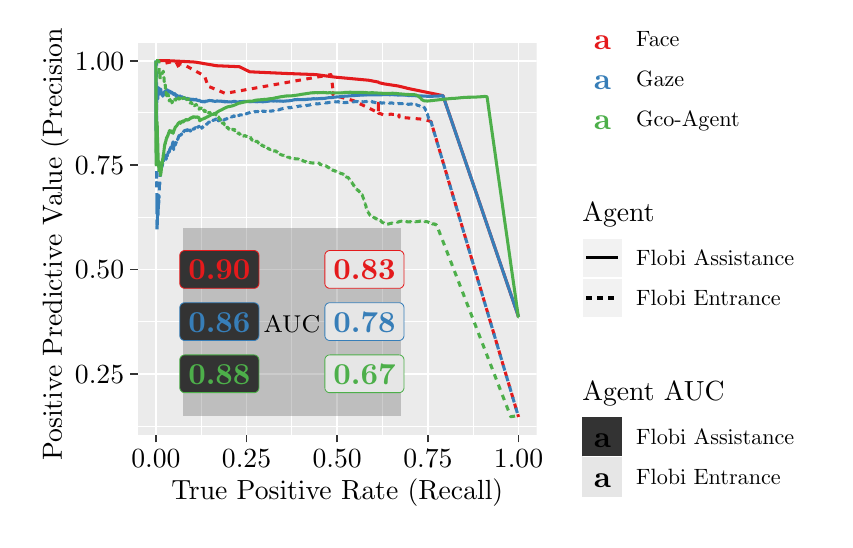
\begin{tikzpicture}[x=1pt,y=1pt]
\definecolor{fillColor}{RGB}{255,255,255}
\path[use as bounding box,fill=fillColor,fill opacity=0.00] (0,0) rectangle (288.00,177.98);
\begin{scope}
\path[clip] (  0.00,  0.00) rectangle (288.00,177.98);
\definecolor{drawColor}{RGB}{255,255,255}
\definecolor{fillColor}{RGB}{255,255,255}

\path[draw=drawColor,line width= 0.6pt,line join=round,line cap=round,fill=fillColor] (  0.00,  0.00) rectangle (288.00,177.98);
\end{scope}
\begin{scope}
\path[clip] ( 39.80, 30.86) rectangle (183.93,172.48);
\definecolor{fillColor}{gray}{0.92}

\path[fill=fillColor] ( 39.80, 30.86) rectangle (183.93,172.48);
\definecolor{drawColor}{RGB}{255,255,255}

\path[draw=drawColor,line width= 0.3pt,line join=round] ( 39.80, 34.05) --
	(183.93, 34.05);

\path[draw=drawColor,line width= 0.3pt,line join=round] ( 39.80, 71.76) --
	(183.93, 71.76);

\path[draw=drawColor,line width= 0.3pt,line join=round] ( 39.80,109.48) --
	(183.93,109.48);

\path[draw=drawColor,line width= 0.3pt,line join=round] ( 39.80,147.19) --
	(183.93,147.19);

\path[draw=drawColor,line width= 0.3pt,line join=round] ( 62.72, 30.86) --
	( 62.72,172.48);

\path[draw=drawColor,line width= 0.3pt,line join=round] ( 95.48, 30.86) --
	( 95.48,172.48);

\path[draw=drawColor,line width= 0.3pt,line join=round] (128.24, 30.86) --
	(128.24,172.48);

\path[draw=drawColor,line width= 0.3pt,line join=round] (161.00, 30.86) --
	(161.00,172.48);

\path[draw=drawColor,line width= 0.6pt,line join=round] ( 39.80, 52.91) --
	(183.93, 52.91);

\path[draw=drawColor,line width= 0.6pt,line join=round] ( 39.80, 90.62) --
	(183.93, 90.62);

\path[draw=drawColor,line width= 0.6pt,line join=round] ( 39.80,128.33) --
	(183.93,128.33);

\path[draw=drawColor,line width= 0.6pt,line join=round] ( 39.80,166.05) --
	(183.93,166.05);

\path[draw=drawColor,line width= 0.6pt,line join=round] ( 46.34, 30.86) --
	( 46.34,172.48);

\path[draw=drawColor,line width= 0.6pt,line join=round] ( 79.10, 30.86) --
	( 79.10,172.48);

\path[draw=drawColor,line width= 0.6pt,line join=round] (111.86, 30.86) --
	(111.86,172.48);

\path[draw=drawColor,line width= 0.6pt,line join=round] (144.62, 30.86) --
	(144.62,172.48);

\path[draw=drawColor,line width= 0.6pt,line join=round] (177.38, 30.86) --
	(177.38,172.48);
\definecolor{fillColor}{RGB}{89,89,89}

\path[fill=fillColor,fill opacity=0.30] ( 56.16, 37.82) rectangle (134.79,105.71);
\definecolor{drawColor}{RGB}{0,0,0}

\node[text=drawColor,anchor=base,inner sep=0pt, outer sep=0pt, scale=  1.10] at ( 95.48, 67.96) {\footnotesize{AUC}};
\definecolor{drawColor}{RGB}{228,26,28}

\path[draw=drawColor,line width= 1.1pt,line join=round] ( 46.53,166.05) --
	( 49.35,166.05) --
	( 49.39,166.05) --
	( 50.69,166.05) --
	( 59.75,165.60) --
	( 59.76,165.60) --
	( 59.77,165.60) --
	( 60.84,165.49) --
	( 68.22,164.23) --
	( 76.43,163.87) --
	( 76.45,163.87) --
	( 76.45,163.87) --
	( 76.47,163.87) --
	( 80.26,162.03) --
	( 93.14,161.44) --
	(103.73,161.04) --
	(104.01,161.04) --
	(104.11,161.03) --
	(110.95,160.12) --
	(123.13,158.99) --
	(126.69,158.33) --
	(126.75,158.27) --
	(126.89,158.12) --
	(128.87,157.66) --
	(133.82,156.91) --
	(136.93,156.17) --
	(137.10,156.09) --
	(150.07,153.42) --
	(177.38, 73.47);

\path[draw=drawColor,line width= 1.1pt,dash pattern=on 2pt off 2pt ,line join=round] ( 46.48,166.05) --
	( 46.76,166.05) --
	( 46.95,166.05) --
	( 48.01,166.05) --
	( 48.68,164.92) --
	( 51.38,165.52) --
	( 52.58,165.62) --
	( 53.48,165.68) --
	( 53.53,165.68) --
	( 53.55,165.68) --
	( 54.96,163.03) --
	( 54.96,165.43) --
	( 63.93,160.52) --
	( 65.25,156.58) --
	( 65.51,156.70) --
	( 71.39,154.23) --
	(109.58,161.02) --
	(109.88,159.19) --
	(110.28,155.83) --
	(110.32,153.67) --
	(110.32,154.52) --
	(111.37,153.34) --
	(117.60,151.66) --
	(126.71,147.26) --
	(126.71,151.06) --
	(126.71,151.44) --
	(126.71,151.52) --
	(126.73,147.01) --
	(127.42,146.93) --
	(128.51,146.46) --
	(130.95,146.64) --
	(130.95,146.76) --
	(132.27,146.62) --
	(134.05,146.69) --
	(134.21,145.60) --
	(134.21,145.97) --
	(134.21,146.47) --
	(136.04,145.46) --
	(143.09,144.87) --
	(145.76,144.07) --
	(145.80,143.84) --
	(177.38, 37.30);
\definecolor{drawColor}{RGB}{55,126,184}

\path[draw=drawColor,line width= 1.1pt,line join=round] ( 46.36,166.05) --
	( 46.37,140.90) --
	( 46.40,150.96) --
	( 46.41,142.84) --
	( 46.43,147.19) --
	( 46.45,150.17) --
	( 46.47,146.37) --
	( 46.49,148.64) --
	( 46.50,145.24) --
	( 46.52,142.48) --
	( 46.54,144.50) --
	( 46.58,147.65) --
	( 46.60,148.90) --
	( 46.62,150.33) --
	( 46.65,151.54) --
	( 46.67,152.33) --
	( 46.69,153.04) --
	( 46.71,153.68) --
	( 46.73,154.26) --
	( 46.75,154.79) --
	( 46.77,155.27) --
	( 46.79,155.71) --
	( 46.81,156.12) --
	( 46.84,156.62) --
	( 46.85,155.14) --
	( 46.87,155.52) --
	( 46.89,155.88) --
	( 46.92,156.31) --
	( 46.93,153.61) --
	( 46.95,153.98) --
	( 46.97,154.33) --
	( 46.98,153.24) --
	( 47.00,152.21) --
	( 47.02,152.70) --
	( 47.04,153.04) --
	( 47.06,153.37) --
	( 47.08,153.68) --
	( 47.10,153.98) --
	( 47.12,154.26) --
	( 47.15,154.62) --
	( 47.17,154.87) --
	( 47.19,155.12) --
	( 47.20,154.28) --
	( 47.23,154.60) --
	( 47.26,154.91) --
	( 47.28,155.20) --
	( 47.30,155.41) --
	( 47.32,155.61) --
	( 47.35,155.87) --
	( 47.37,156.05) --
	( 47.39,156.23) --
	( 47.40,155.52) --
	( 47.42,155.70) --
	( 47.45,155.93) --
	( 47.46,154.44) --
	( 47.48,154.69) --
	( 47.51,154.93) --
	( 47.53,154.38) --
	( 47.56,154.62) --
	( 47.58,154.10) --
	( 47.60,154.27) --
	( 47.62,154.44) --
	( 47.64,153.95) --
	( 47.66,154.12) --
	( 47.69,154.39) --
	( 47.71,154.55) --
	( 47.73,154.70) --
	( 47.76,154.90) --
	( 47.78,155.09) --
	( 47.80,155.23) --
	( 47.82,155.36) --
	( 47.84,154.87) --
	( 47.86,155.05) --
	( 47.88,155.19) --
	( 47.91,155.36) --
	( 47.94,155.52) --
	( 47.95,155.07) --
	( 47.98,155.27) --
	( 48.00,155.39) --
	( 48.02,155.51) --
	( 48.05,155.66) --
	( 48.08,155.81) --
	( 48.10,154.93) --
	( 48.12,155.05) --
	( 48.14,155.16) --
	( 48.16,155.27) --
	( 48.18,154.91) --
	( 48.19,154.52) --
	( 48.21,154.63) --
	( 48.23,154.75) --
	( 48.25,154.41) --
	( 48.27,154.52) --
	( 48.29,154.63) --
	( 48.30,154.26) --
	( 48.32,154.37) --
	( 48.34,154.48) --
	( 48.37,154.62) --
	( 48.39,154.72) --
	( 48.40,154.37) --
	( 48.42,154.07) --
	( 48.44,154.17) --
	( 48.46,154.27) --
	( 48.48,153.94) --
	( 48.49,153.62) --
	( 48.51,153.72) --
	( 48.53,153.83) --
	( 48.54,153.51) --
	( 48.57,153.65) --
	( 48.59,153.75) --
	( 48.61,153.85) --
	( 48.63,153.58) --
	( 48.65,153.68) --
	( 48.67,153.77) --
	( 48.69,153.51) --
	( 48.71,153.61) --
	( 48.72,153.31) --
	( 48.74,153.41) --
	( 48.76,153.51) --
	( 48.78,153.26) --
	( 48.80,153.35) --
	( 48.82,153.44) --
	( 48.84,153.20) --
	( 48.86,153.29) --
	( 48.88,153.39) --
	( 48.90,153.48) --
	( 48.92,153.56) --
	( 48.94,153.65) --
	( 48.96,153.42) --
	( 48.98,153.50) --
	( 49.01,153.62) --
	( 49.05,153.79) --
	( 49.08,153.90) --
	( 49.09,153.64) --
	( 49.12,153.75) --
	( 49.14,153.83) --
	( 49.16,153.94) --
	( 49.18,153.69) --
	( 49.20,153.77) --
	( 49.22,153.85) --
	( 49.24,153.93) --
	( 49.26,154.03) --
	( 49.28,154.10) --
	( 49.30,154.18) --
	( 49.33,154.28) --
	( 49.36,154.37) --
	( 49.38,154.44) --
	( 49.40,154.51) --
	( 49.42,154.60) --
	( 49.45,154.70) --
	( 49.47,154.76) --
	( 49.49,154.83) --
	( 49.51,154.89) --
	( 49.53,154.96) --
	( 49.55,155.02) --
	( 49.57,154.80) --
	( 49.59,154.86) --
	( 49.60,154.64) --
	( 49.62,154.70) --
	( 49.65,154.81) --
	( 49.67,154.59) --
	( 49.69,154.66) --
	( 49.71,154.72) --
	( 49.72,154.51) --
	( 49.75,154.59) --
	( 49.77,154.65) --
	( 49.79,154.73) --
	( 49.81,154.28) --
	( 49.83,154.34) --
	( 49.85,154.40) --
	( 49.87,154.46) --
	( 49.89,154.52) --
	( 49.91,154.60) --
	( 49.93,154.40) --
	( 49.95,154.46) --
	( 49.97,154.52) --
	( 49.99,154.58) --
	( 50.01,154.64) --
	( 50.03,154.69) --
	( 50.04,154.50) --
	( 50.06,154.56) --
	( 50.08,154.61) --
	( 50.10,154.67) --
	( 50.13,154.75) --
	( 50.15,154.82) --
	( 50.17,154.87) --
	( 50.19,154.93) --
	( 50.21,154.98) --
	( 50.23,155.03) --
	( 50.27,155.14) --
	( 50.29,155.19) --
	( 50.31,155.24) --
	( 50.33,155.29) --
	( 50.35,155.34) --
	( 50.37,155.39) --
	( 50.39,155.44) --
	( 50.42,155.50) --
	( 50.43,155.32) --
	( 50.45,155.37) --
	( 50.48,155.43) --
	( 50.50,155.48) --
	( 50.52,155.53) --
	( 50.53,155.35) --
	( 50.55,155.18) --
	( 50.56,155.00) --
	( 50.57,154.83) --
	( 50.59,154.66) --
	( 50.61,154.71) --
	( 50.63,154.76) --
	( 50.65,154.81) --
	( 50.66,154.64) --
	( 50.70,154.74) --
	( 50.73,154.80) --
	( 50.74,154.64) --
	( 50.76,154.69) --
	( 50.78,154.73) --
	( 50.80,154.78) --
	( 50.82,154.83) --
	( 50.84,154.87) --
	( 50.86,154.92) --
	( 50.88,154.96) --
	( 50.90,155.01) --
	( 50.92,155.05) --
	( 50.94,155.10) --
	( 50.96,155.14) --
	( 50.99,155.20) --
	( 51.00,155.04) --
	( 51.02,155.09) --
	( 51.03,154.93) --
	( 51.05,154.97) --
	( 51.07,155.02) --
	( 51.09,155.06) --
	( 51.11,155.10) --
	( 51.13,154.97) --
	( 51.15,155.01) --
	( 51.17,154.86) --
	( 51.19,154.92) --
	( 51.21,154.77) --
	( 51.23,154.81) --
	( 51.25,154.85) --
	( 51.27,154.89) --
	( 51.28,154.75) --
	( 51.30,154.79) --
	( 51.33,154.84) --
	( 51.35,154.71) --
	( 51.37,154.77) --
	( 51.39,154.81) --
	( 51.41,154.67) --
	( 51.43,154.71) --
	( 51.45,154.76) --
	( 51.48,154.82) --
	( 51.50,154.86) --
	( 51.52,154.90) --
	( 51.54,154.94) --
	( 51.56,154.98) --
	( 51.58,154.69) --
	( 51.59,154.55) --
	( 51.61,154.59) --
	( 51.63,154.46) --
	( 51.65,154.50) --
	( 51.67,154.38) --
	( 51.69,154.43) --
	( 51.71,154.47) --
	( 51.74,154.52) --
	( 51.77,154.57) --
	( 51.78,154.44) --
	( 51.80,154.48) --
	( 51.82,154.52) --
	( 51.84,154.56) --
	( 51.86,154.44) --
	( 51.88,154.48) --
	( 51.89,154.35) --
	( 51.93,154.42) --
	( 51.95,154.46) --
	( 51.97,154.51) --
	( 51.99,154.54) --
	( 52.01,154.58) --
	( 52.04,154.63) --
	( 52.07,154.68) --
	( 52.08,154.55) --
	( 52.11,154.60) --
	( 52.12,154.48) --
	( 52.13,154.36) --
	( 52.16,154.41) --
	( 52.18,154.44) --
	( 52.20,154.48) --
	( 52.23,154.53) --
	( 52.24,154.41) --
	( 52.26,154.44) --
	( 52.28,154.48) --
	( 52.30,154.51) --
	( 52.31,154.24) --
	( 52.33,154.28) --
	( 52.35,154.31) --
	( 52.36,154.19) --
	( 52.37,154.08) --
	( 52.39,154.11) --
	( 52.41,154.15) --
	( 52.43,154.19) --
	( 52.45,154.08) --
	( 52.48,154.13) --
	( 52.51,154.04) --
	( 52.53,154.07) --
	( 52.55,153.97) --
	( 52.57,154.01) --
	( 52.59,154.06) --
	( 52.61,154.09) --
	( 52.64,154.14) --
	( 52.66,154.17) --
	( 52.69,154.22) --
	( 52.70,154.11) --
	( 52.72,154.14) --
	( 52.73,154.03) --
	( 52.75,154.07) --
	( 52.77,153.96) --
	( 52.78,153.85) --
	( 52.80,153.88) --
	( 52.82,153.92) --
	( 52.84,153.95) --
	( 52.87,154.00) --
	( 52.88,153.89) --
	( 52.91,153.93) --
	( 52.93,153.98) --
	( 52.96,154.02) --
	( 52.98,154.06) --
	( 53.00,154.09) --
	( 53.02,154.12) --
	( 53.03,154.02) --
	( 53.05,154.05) --
	( 53.07,154.08) --
	( 53.10,154.13) --
	( 53.12,154.16) --
	( 53.14,153.94) --
	( 53.16,153.97) --
	( 53.19,154.02) --
	( 53.21,154.05) --
	( 53.22,153.95) --
	( 53.24,153.98) --
	( 53.26,154.01) --
	( 53.28,154.04) --
	( 53.31,154.08) --
	( 53.33,153.99) --
	( 53.35,153.90) --
	( 53.38,153.96) --
	( 53.40,153.86) --
	( 53.41,153.76) --
	( 53.43,153.79) --
	( 53.45,153.82) --
	( 53.48,153.86) --
	( 53.50,153.66) --
	( 53.52,153.70) --
	( 53.54,153.60) --
	( 53.56,153.64) --
	( 53.58,153.67) --
	( 53.58,153.44) --
	( 53.59,153.22) --
	( 53.61,153.25) --
	( 53.62,153.16) --
	( 53.65,153.20) --
	( 53.68,153.26) --
	( 53.70,153.17) --
	( 53.72,153.21) --
	( 53.74,153.24) --
	( 53.76,153.27) --
	( 53.78,153.18) --
	( 53.80,153.21) --
	( 53.82,153.25) --
	( 53.84,153.28) --
	( 53.87,153.32) --
	( 53.90,153.36) --
	( 53.92,153.39) --
	( 53.94,153.43) --
	( 53.96,153.47) --
	( 53.99,153.51) --
	( 54.01,153.43) --
	( 54.02,153.23) --
	( 54.04,153.26) --
	( 54.06,153.17) --
	( 54.08,153.20) --
	( 54.10,153.23) --
	( 54.11,153.14) --
	( 54.13,153.06) --
	( 54.15,153.09) --
	( 54.16,153.01) --
	( 54.18,153.04) --
	( 54.21,153.08) --
	( 54.22,152.99) --
	( 54.24,153.02) --
	( 54.27,153.06) --
	( 54.29,153.09) --
	( 54.30,153.00) --
	( 54.33,153.04) --
	( 54.35,153.07) --
	( 54.37,153.10) --
	( 54.39,153.13) --
	( 54.41,153.16) --
	( 54.43,153.19) --
	( 54.45,153.22) --
	( 54.47,153.25) --
	( 54.49,153.28) --
	( 54.50,153.19) --
	( 54.52,153.22) --
	( 54.54,153.25) --
	( 54.56,153.28) --
	( 54.58,153.20) --
	( 54.60,153.23) --
	( 54.62,153.15) --
	( 54.64,153.18) --
	( 54.66,153.21) --
	( 54.67,153.13) --
	( 54.69,153.05) --
	( 54.71,152.98) --
	( 54.76,153.05) --
	( 54.78,153.08) --
	( 54.80,153.11) --
	( 54.82,153.14) --
	( 54.84,153.17) --
	( 54.87,153.21) --
	( 54.89,153.13) --
	( 54.92,153.17) --
	( 54.94,153.20) --
	( 54.96,153.23) --
	( 54.98,153.25) --
	( 55.00,153.28) --
	( 55.02,153.31) --
	( 55.03,153.23) --
	( 55.05,153.16) --
	( 55.06,153.08) --
	( 55.08,153.11) --
	( 55.10,153.04) --
	( 55.12,152.96) --
	( 55.14,152.99) --
	( 55.15,152.82) --
	( 55.18,152.85) --
	( 55.20,152.88) --
	( 55.22,152.91) --
	( 55.23,152.83) --
	( 55.25,152.86) --
	( 55.26,152.78) --
	( 55.28,152.81) --
	( 55.30,152.84) --
	( 55.32,152.86) --
	( 55.35,152.90) --
	( 55.37,152.92) --
	( 55.40,152.96) --
	( 55.42,152.99) --
	( 55.43,152.91) --
	( 55.45,152.94) --
	( 55.46,152.86) --
	( 55.48,152.89) --
	( 55.50,152.92) --
	( 55.52,152.94) --
	( 55.54,152.97) --
	( 55.57,153.00) --
	( 55.59,152.94) --
	( 55.61,152.96) --
	( 55.63,152.99) --
	( 55.65,153.01) --
	( 55.68,153.05) --
	( 55.69,152.98) --
	( 55.70,152.90) --
	( 55.73,152.94) --
	( 55.75,152.96) --
	( 55.77,152.99) --
	( 55.78,152.92) --
	( 55.80,152.94) --
	( 55.81,152.68) --
	( 55.83,152.71) --
	( 55.85,152.74) --
	( 55.88,152.77) --
	( 55.90,152.80) --
	( 55.92,152.82) --
	( 55.94,152.85) --
	( 55.96,152.87) --
	( 55.98,152.90) --
	( 56.00,152.92) --
	( 56.03,152.88) --
	( 56.05,152.81) --
	( 56.07,152.84) --
	( 56.08,152.77) --
	( 56.10,152.71) --
	( 56.13,152.74) --
	( 56.14,152.67) --
	( 56.16,152.70) --
	( 56.18,152.72) --
	( 56.20,152.48) --
	( 56.21,152.42) --
	( 56.23,152.44) --
	( 56.26,152.48) --
	( 56.27,152.41) --
	( 56.30,152.44) --
	( 56.32,152.47) --
	( 56.34,152.49) --
	( 56.36,152.52) --
	( 56.38,152.54) --
	( 56.40,152.56) --
	( 56.42,152.60) --
	( 56.43,152.44) --
	( 56.46,152.47) --
	( 56.48,152.50) --
	( 56.50,152.52) --
	( 56.52,152.55) --
	( 56.54,152.57) --
	( 56.56,152.59) --
	( 56.58,152.62) --
	( 56.60,152.64) --
	( 56.62,152.67) --
	( 56.64,152.70) --
	( 56.66,152.72) --
	( 56.68,152.66) --
	( 56.70,152.68) --
	( 56.72,152.62) --
	( 56.73,152.56) --
	( 56.75,152.58) --
	( 56.77,152.60) --
	( 56.78,152.45) --
	( 56.80,152.48) --
	( 56.81,152.41) --
	( 56.83,152.44) --
	( 56.85,152.46) --
	( 56.88,152.50) --
	( 56.90,152.52) --
	( 56.92,152.46) --
	( 56.94,152.48) --
	( 56.95,152.42) --
	( 56.96,152.27) --
	( 56.98,152.29) --
	( 57.00,152.33) --
	( 57.02,152.35) --
	( 57.04,152.37) --
	( 57.06,152.31) --
	( 57.07,152.25) --
	( 57.09,152.27) --
	( 57.11,152.29) --
	( 57.13,152.32) --
	( 57.14,152.26) --
	( 57.16,152.28) --
	( 57.18,152.30) --
	( 57.20,152.33) --
	( 57.23,152.36) --
	( 57.25,152.38) --
	( 57.27,152.32) --
	( 57.29,152.34) --
	( 57.32,152.38) --
	( 57.33,152.23) --
	( 57.35,152.26) --
	( 57.38,152.30) --
	( 57.41,152.33) --
	( 57.43,152.35) --
	( 57.45,152.37) --
	( 57.47,152.40) --
	( 57.49,152.42) --
	( 57.51,152.44) --
	( 57.53,152.38) --
	( 57.55,152.41) --
	( 57.57,152.44) --
	( 57.59,152.46) --
	( 57.61,152.40) --
	( 57.63,152.42) --
	( 57.64,152.36) --
	( 57.66,152.38) --
	( 57.68,152.41) --
	( 57.70,152.43) --
	( 57.72,152.45) --
	( 57.73,152.39) --
	( 57.75,152.34) --
	( 57.78,152.37) --
	( 57.80,152.39) --
	( 57.81,152.33) --
	( 57.83,152.35) --
	( 57.84,152.22) --
	( 57.86,152.24) --
	( 57.88,152.26) --
	( 57.90,152.28) --
	( 57.91,152.23) --
	( 57.94,152.25) --
	( 57.96,152.28) --
	( 57.98,152.30) --
	( 57.99,152.24) --
	( 58.02,152.27) --
	( 58.04,152.29) --
	( 58.05,152.16) --
	( 58.07,152.18) --
	( 58.09,152.20) --
	( 58.11,152.22) --
	( 58.12,152.16) --
	( 58.13,152.11) --
	( 58.17,152.14) --
	( 58.19,152.16) --
	( 58.21,152.19) --
	( 58.22,152.13) --
	( 58.24,152.15) --
	( 58.27,152.18) --
	( 58.29,152.21) --
	( 58.32,152.24) --
	( 58.33,152.04) --
	( 58.35,152.06) --
	( 58.37,152.08) --
	( 58.39,152.11) --
	( 58.41,152.13) --
	( 58.43,152.15) --
	( 58.45,152.17) --
	( 58.48,152.20) --
	( 58.49,152.07) --
	( 58.51,152.09) --
	( 58.53,152.11) --
	( 58.55,152.14) --
	( 58.57,152.08) --
	( 58.59,152.10) --
	( 58.61,152.13) --
	( 58.64,152.16) --
	( 58.65,152.10) --
	( 58.68,152.13) --
	( 58.70,152.15) --
	( 58.72,152.10) --
	( 58.74,152.13) --
	( 58.76,152.15) --
	( 58.77,152.09) --
	( 58.79,152.04) --
	( 58.81,152.07) --
	( 58.83,152.02) --
	( 58.86,152.05) --
	( 58.87,152.00) --
	( 58.89,151.94) --
	( 58.91,151.96) --
	( 58.93,151.98) --
	( 58.95,152.00) --
	( 58.97,152.03) --
	( 58.99,151.98) --
	( 59.01,152.01) --
	( 59.03,152.03) --
	( 59.06,152.05) --
	( 59.08,152.07) --
	( 59.10,152.09) --
	( 59.13,152.12) --
	( 59.15,152.14) --
	( 59.17,152.16) --
	( 59.19,152.18) --
	( 59.19,152.06) --
	( 59.22,152.08) --
	( 59.23,152.03) --
	( 59.24,151.91) --
	( 59.26,151.93) --
	( 59.29,151.95) --
	( 59.31,151.97) --
	( 59.33,151.99) --
	( 59.35,152.01) --
	( 59.36,151.96) --
	( 59.39,152.00) --
	( 59.41,151.95) --
	( 59.42,151.90) --
	( 59.44,151.92) --
	( 59.46,151.93) --
	( 59.49,151.90) --
	( 59.51,151.92) --
	( 59.53,151.94) --
	( 59.55,151.96) --
	( 59.57,151.98) --
	( 59.60,152.01) --
	( 59.61,151.96) --
	( 59.63,151.98) --
	( 59.65,152.00) --
	( 59.68,152.02) --
	( 59.70,152.04) --
	( 59.72,152.06) --
	( 59.74,152.08) --
	( 59.76,152.10) --
	( 59.78,152.12) --
	( 59.80,152.14) --
	( 59.81,152.02) --
	( 59.83,151.98) --
	( 59.85,152.00) --
	( 59.86,151.95) --
	( 59.87,151.90) --
	( 59.89,151.92) --
	( 59.91,151.87) --
	( 59.93,151.89) --
	( 59.95,151.91) --
	( 59.97,151.93) --
	( 59.99,151.88) --
	( 60.00,151.84) --
	( 60.02,151.85) --
	( 60.04,151.87) --
	( 60.05,151.83) --
	( 60.07,151.84) --
	( 60.09,151.86) --
	( 60.12,151.89) --
	( 60.14,151.91) --
	( 60.16,151.87) --
	( 60.18,151.88) --
	( 60.20,151.90) --
	( 60.21,151.85) --
	( 60.24,151.88) --
	( 60.25,151.83) --
	( 60.27,151.85) --
	( 60.29,151.87) --
	( 60.31,151.89) --
	( 60.34,151.91) --
	( 60.37,151.94) --
	( 60.39,151.95) --
	( 60.41,151.97) --
	( 60.43,151.99) --
	( 60.44,151.94) --
	( 60.46,151.96) --
	( 60.48,151.98) --
	( 60.50,152.00) --
	( 60.53,152.02) --
	( 60.54,151.92) --
	( 60.55,151.87) --
	( 60.58,151.90) --
	( 60.60,151.91) --
	( 60.62,151.93) --
	( 60.64,151.95) --
	( 60.68,151.99) --
	( 60.70,151.95) --
	( 60.72,151.96) --
	( 60.74,151.98) --
	( 60.76,152.00) --
	( 60.78,152.02) --
	( 60.80,152.03) --
	( 60.83,152.06) --
	( 60.86,152.09) --
	( 60.88,152.10) --
	( 60.91,152.13) --
	( 60.92,152.08) --
	( 60.92,151.86) --
	( 60.94,151.87) --
	( 60.96,151.89) --
	( 60.98,151.91) --
	( 60.99,151.86) --
	( 61.01,151.88) --
	( 61.03,151.84) --
	( 61.05,151.74) --
	( 61.07,151.76) --
	( 61.09,151.78) --
	( 61.13,151.81) --
	( 61.14,151.77) --
	( 61.17,151.79) --
	( 61.19,151.81) --
	( 61.21,151.83) --
	( 61.22,151.78) --
	( 61.25,151.80) --
	( 61.27,151.77) --
	( 61.29,151.78) --
	( 61.31,151.75) --
	( 61.33,151.76) --
	( 61.34,151.72) --
	( 61.36,151.74) --
	( 61.38,151.69) --
	( 61.40,151.72) --
	( 61.42,151.67) --
	( 61.44,151.70) --
	( 61.46,151.71) --
	( 61.48,151.67) --
	( 61.51,151.70) --
	( 61.53,151.72) --
	( 61.55,151.73) --
	( 61.57,151.75) --
	( 61.58,151.71) --
	( 61.60,151.73) --
	( 61.62,151.68) --
	( 61.64,151.70) --
	( 61.66,151.72) --
	( 61.68,151.73) --
	( 61.71,151.76) --
	( 61.74,151.78) --
	( 61.75,151.74) --
	( 61.76,151.64) --
	( 61.78,151.66) --
	( 61.80,151.67) --
	( 61.83,151.70) --
	( 61.85,151.72) --
	( 61.86,151.68) --
	( 61.88,151.69) --
	( 61.90,151.65) --
	( 61.92,151.56) --
	( 61.94,151.59) --
	( 61.96,151.60) --
	( 61.98,151.62) --
	( 62.00,151.64) --
	( 62.02,151.65) --
	( 62.05,151.67) --
	( 62.08,151.70) --
	( 62.10,151.72) --
	( 62.12,151.68) --
	( 62.14,151.64) --
	( 62.16,151.61) --
	( 62.17,151.56) --
	( 62.19,151.58) --
	( 62.21,151.55) --
	( 62.23,151.56) --
	( 62.24,151.52) --
	( 62.27,151.54) --
	( 62.29,151.56) --
	( 62.31,151.58) --
	( 62.33,151.54) --
	( 62.35,151.51) --
	( 62.37,151.52) --
	( 62.38,151.43) --
	( 62.40,151.44) --
	( 62.43,151.47) --
	( 62.45,151.49) --
	( 62.47,151.50) --
	( 62.50,151.52) --
	( 62.50,151.38) --
	( 62.52,151.34) --
	( 62.55,151.36) --
	( 62.57,151.38) --
	( 62.59,151.35) --
	( 62.63,151.38) --
	( 62.64,151.34) --
	( 62.66,151.30) --
	( 62.68,151.32) --
	( 62.69,151.28) --
	( 62.71,151.29) --
	( 62.73,151.31) --
	( 62.75,151.33) --
	( 62.76,151.29) --
	( 62.78,151.30) --
	( 62.80,151.32) --
	( 62.83,151.34) --
	( 62.86,151.36) --
	( 62.88,151.38) --
	( 62.89,151.29) --
	( 62.90,151.20) --
	( 62.93,151.22) --
	( 62.94,151.19) --
	( 62.96,151.20) --
	( 62.99,151.22) --
	( 63.01,151.24) --
	( 63.04,151.26) --
	( 63.05,151.22) --
	( 63.07,151.19) --
	( 63.09,151.21) --
	( 63.11,151.22) --
	( 63.14,151.24) --
	( 63.16,151.26) --
	( 63.18,151.28) --
	( 63.20,151.30) --
	( 63.22,151.31) --
	( 63.25,151.33) --
	( 63.27,151.35) --
	( 63.30,151.37) --
	( 63.32,151.34) --
	( 63.34,151.36) --
	( 63.36,151.32) --
	( 63.38,151.33) --
	( 63.40,151.36) --
	( 63.42,151.32) --
	( 63.43,151.28) --
	( 63.47,151.31) --
	( 63.49,151.33) --
	( 63.52,151.35) --
	( 63.54,151.37) --
	( 63.55,151.28) --
	( 63.57,151.29) --
	( 63.59,151.31) --
	( 63.62,151.33) --
	( 63.64,151.34) --
	( 63.66,151.36) --
	( 63.66,151.27) --
	( 63.69,151.29) --
	( 63.72,151.31) --
	( 63.74,151.33) --
	( 63.75,151.29) --
	( 63.76,151.25) --
	( 63.78,151.22) --
	( 63.79,151.13) --
	( 63.81,151.15) --
	( 63.83,151.16) --
	( 63.84,151.13) --
	( 63.87,151.15) --
	( 63.89,151.16) --
	( 63.90,151.13) --
	( 63.94,151.15) --
	( 63.96,151.17) --
	( 63.98,151.18) --
	( 64.00,151.20) --
	( 64.02,151.21) --
	( 64.04,151.23) --
	( 64.07,151.25) --
	( 64.09,151.27) --
	( 64.12,151.29) --
	( 64.14,151.30) --
	( 64.16,151.32) --
	( 64.17,151.24) --
	( 64.19,151.25) --
	( 64.22,151.27) --
	( 64.24,151.29) --
	( 64.26,151.30) --
	( 64.28,151.32) --
	( 64.30,151.33) --
	( 64.32,151.35) --
	( 64.34,151.37) --
	( 64.37,151.38) --
	( 64.40,151.40) --
	( 64.42,151.42) --
	( 64.44,151.44) --
	( 64.46,151.45) --
	( 64.48,151.42) --
	( 64.50,151.44) --
	( 64.54,151.46) --
	( 64.56,151.48) --
	( 64.57,151.44) --
	( 64.59,151.45) --
	( 64.61,151.42) --
	( 64.63,151.44) --
	( 64.65,151.45) --
	( 64.67,151.42) --
	( 64.69,151.44) --
	( 64.72,151.46) --
	( 64.74,151.47) --
	( 64.75,151.44) --
	( 64.77,151.45) --
	( 64.78,151.41) --
	( 64.80,151.43) --
	( 64.82,151.44) --
	( 64.84,151.41) --
	( 64.86,151.43) --
	( 64.88,151.40) --
	( 64.90,151.41) --
	( 64.92,151.43) --
	( 64.95,151.44) --
	( 64.98,151.46) --
	( 65.00,151.48) --
	( 65.03,151.50) --
	( 65.05,151.52) --
	( 65.08,151.53) --
	( 65.10,151.55) --
	( 65.12,151.56) --
	( 65.14,151.58) --
	( 65.16,151.59) --
	( 65.17,151.56) --
	( 65.19,151.57) --
	( 65.21,151.54) --
	( 65.23,151.55) --
	( 65.25,151.57) --
	( 65.28,151.59) --
	( 65.31,151.60) --
	( 65.33,151.62) --
	( 65.35,151.64) --
	( 65.39,151.66) --
	( 65.41,151.67) --
	( 65.43,151.69) --
	( 65.44,151.61) --
	( 65.47,151.63) --
	( 65.49,151.64) --
	( 65.50,151.56) --
	( 65.52,151.58) --
	( 65.54,151.55) --
	( 65.56,151.56) --
	( 65.59,151.58) --
	( 65.61,151.59) --
	( 65.63,151.61) --
	( 65.65,151.62) --
	( 65.67,151.64) --
	( 65.69,151.65) --
	( 65.71,151.67) --
	( 65.74,151.68) --
	( 65.75,151.65) --
	( 65.76,151.57) --
	( 65.79,151.59) --
	( 65.81,151.61) --
	( 65.84,151.62) --
	( 65.87,151.64) --
	( 65.89,151.66) --
	( 65.91,151.67) --
	( 65.93,151.69) --
	( 65.95,151.70) --
	( 65.97,151.71) --
	( 65.99,151.73) --
	( 66.01,151.74) --
	( 66.03,151.71) --
	( 66.05,151.72) --
	( 66.07,151.70) --
	( 66.09,151.71) --
	( 66.11,151.68) --
	( 66.13,151.65) --
	( 66.15,151.66) --
	( 66.17,151.67) --
	( 66.19,151.69) --
	( 66.21,151.70) --
	( 66.23,151.67) --
	( 66.25,151.64) --
	( 66.27,151.66) --
	( 66.29,151.67) --
	( 66.31,151.64) --
	( 66.32,151.61) --
	( 66.35,151.63) --
	( 66.37,151.64) --
	( 66.38,151.61) --
	( 66.40,151.62) --
	( 66.42,151.63) --
	( 66.44,151.65) --
	( 66.46,151.66) --
	( 66.47,151.63) --
	( 66.49,151.64) --
	( 66.51,151.57) --
	( 66.53,151.58) --
	( 66.54,151.55) --
	( 66.56,151.56) --
	( 66.58,151.53) --
	( 66.60,151.55) --
	( 66.62,151.56) --
	( 66.64,151.53) --
	( 66.66,151.50) --
	( 66.68,151.52) --
	( 66.71,151.53) --
	( 66.75,151.56) --
	( 66.77,151.58) --
	( 66.79,151.54) --
	( 66.81,151.56) --
	( 66.83,151.57) --
	( 66.83,151.49) --
	( 66.85,151.46) --
	( 66.87,151.48) --
	( 66.89,151.49) --
	( 66.91,151.46) --
	( 66.93,151.47) --
	( 66.95,151.49) --
	( 66.97,151.46) --
	( 66.99,151.47) --
	( 67.01,151.48) --
	( 67.03,151.50) --
	( 67.04,151.47) --
	( 67.05,151.44) --
	( 67.07,151.45) --
	( 67.09,151.46) --
	( 67.11,151.43) --
	( 67.15,151.46) --
	( 67.17,151.43) --
	( 67.19,151.45) --
	( 67.21,151.41) --
	( 67.23,151.43) --
	( 67.23,151.35) --
	( 67.26,151.37) --
	( 67.29,151.39) --
	( 67.31,151.36) --
	( 67.33,151.37) --
	( 67.35,151.39) --
	( 67.38,151.37) --
	( 67.39,151.34) --
	( 67.42,151.35) --
	( 67.44,151.37) --
	( 67.47,151.38) --
	( 67.49,151.40) --
	( 67.51,151.41) --
	( 67.53,151.42) --
	( 67.55,151.39) --
	( 67.57,151.41) --
	( 67.59,151.42) --
	( 67.61,151.35) --
	( 67.62,151.32) --
	( 67.65,151.34) --
	( 67.67,151.35) --
	( 67.69,151.37) --
	( 67.71,151.38) --
	( 67.73,151.39) --
	( 67.74,151.32) --
	( 67.76,151.33) --
	( 67.77,151.30) --
	( 67.80,151.32) --
	( 67.83,151.34) --
	( 67.85,151.35) --
	( 67.87,151.32) --
	( 67.89,151.34) --
	( 67.91,151.35) --
	( 67.94,151.37) --
	( 67.96,151.38) --
	( 67.97,151.35) --
	( 68.00,151.37) --
	( 68.02,151.38) --
	( 68.04,151.39) --
	( 68.06,151.40) --
	( 68.09,151.43) --
	( 68.11,151.40) --
	( 68.13,151.41) --
	( 68.15,151.42) --
	( 68.17,151.43) --
	( 68.18,151.40) --
	( 68.20,151.41) --
	( 68.22,151.43) --
	( 68.25,151.44) --
	( 68.27,151.46) --
	( 68.30,151.47) --
	( 68.32,151.49) --
	( 68.34,151.50) --
	( 68.36,151.51) --
	( 68.39,151.53) --
	( 68.41,151.54) --
	( 68.43,151.51) --
	( 68.45,151.53) --
	( 68.47,151.54) --
	( 68.49,151.55) --
	( 68.50,151.48) --
	( 68.52,151.46) --
	( 68.55,151.47) --
	( 68.57,151.48) --
	( 68.59,151.50) --
	( 68.61,151.43) --
	( 68.63,151.45) --
	( 68.65,151.46) --
	( 68.67,151.43) --
	( 68.69,151.45) --
	( 68.70,151.42) --
	( 68.72,151.43) --
	( 68.74,151.44) --
	( 68.77,151.46) --
	( 68.78,151.43) --
	( 68.80,151.44) --
	( 68.82,151.45) --
	( 68.86,151.47) --
	( 68.88,151.48) --
	( 68.89,151.45) --
	( 68.90,151.42) --
	( 68.93,151.44) --
	( 68.96,151.46) --
	( 68.98,151.43) --
	( 68.99,151.37) --
	( 69.02,151.38) --
	( 69.04,151.39) --
	( 69.06,151.41) --
	( 69.08,151.38) --
	( 69.10,151.36) --
	( 69.12,151.37) --
	( 69.14,151.38) --
	( 69.16,151.40) --
	( 69.18,151.41) --
	( 69.22,151.43) --
	( 69.25,151.45) --
	( 69.27,151.46) --
	( 69.30,151.47) --
	( 69.31,151.44) --
	( 69.33,151.46) --
	( 69.34,151.43) --
	( 69.36,151.40) --
	( 69.38,151.41) --
	( 69.41,151.43) --
	( 69.43,151.44) --
	( 69.44,151.41) --
	( 69.47,151.43) --
	( 69.49,151.44) --
	( 69.52,151.46) --
	( 69.54,151.47) --
	( 69.57,151.49) --
	( 69.58,151.46) --
	( 69.60,151.43) --
	( 69.62,151.44) --
	( 69.63,151.41) --
	( 69.64,151.39) --
	( 69.66,151.40) --
	( 69.68,151.37) --
	( 69.70,151.38) --
	( 69.72,151.39) --
	( 69.74,151.40) --
	( 69.76,151.42) --
	( 69.77,151.39) --
	( 69.80,151.40) --
	( 69.82,151.41) --
	( 69.84,151.43) --
	( 69.86,151.44) --
	( 69.90,151.46) --
	( 69.92,151.44) --
	( 69.94,151.45) --
	( 69.96,151.46) --
	( 69.98,151.47) --
	( 70.00,151.41) --
	( 70.02,151.35) --
	( 70.05,151.37) --
	( 70.07,151.38) --
	( 70.10,151.40) --
	( 70.11,151.37) --
	( 70.14,151.39) --
	( 70.16,151.40) --
	( 70.18,151.41) --
	( 70.20,151.42) --
	( 70.21,151.39) --
	( 70.23,151.40) --
	( 70.25,151.41) --
	( 70.26,151.39) --
	( 70.28,151.36) --
	( 70.29,151.33) --
	( 70.32,151.35) --
	( 70.34,151.36) --
	( 70.36,151.34) --
	( 70.38,151.35) --
	( 70.40,151.36) --
	( 70.41,151.33) --
	( 70.44,151.31) --
	( 70.46,151.32) --
	( 70.47,151.30) --
	( 70.49,151.31) --
	( 70.52,151.32) --
	( 70.54,151.33) --
	( 70.56,151.34) --
	( 70.57,151.32) --
	( 70.58,151.29) --
	( 70.60,151.30) --
	( 70.61,151.24) --
	( 70.63,151.25) --
	( 70.65,151.26) --
	( 70.66,151.23) --
	( 70.68,151.21) --
	( 70.70,151.22) --
	( 70.72,151.23) --
	( 70.75,151.25) --
	( 70.78,151.27) --
	( 70.80,151.28) --
	( 70.82,151.29) --
	( 70.84,151.30) --
	( 70.86,151.31) --
	( 70.88,151.28) --
	( 70.90,151.30) --
	( 70.92,151.31) --
	( 70.94,151.32) --
	( 70.96,151.33) --
	( 70.99,151.34) --
	( 71.04,151.37) --
	( 71.06,151.38) --
	( 71.08,151.39) --
	( 71.10,151.34) --
	( 71.12,151.35) --
	( 71.13,151.29) --
	( 71.15,151.30) --
	( 71.18,151.31) --
	( 71.18,151.25) --
	( 71.20,151.26) --
	( 71.22,151.27) --
	( 71.24,151.15) --
	( 71.26,151.16) --
	( 71.28,151.17) --
	( 71.30,151.18) --
	( 71.32,151.19) --
	( 71.34,151.20) --
	( 71.34,151.14) --
	( 71.36,151.15) --
	( 71.38,151.12) --
	( 71.39,151.10) --
	( 71.42,151.11) --
	( 71.44,151.13) --
	( 71.46,151.14) --
	( 71.48,151.15) --
	( 71.51,151.16) --
	( 71.54,151.18) --
	( 71.55,151.15) --
	( 71.58,151.17) --
	( 71.60,151.18) --
	( 71.62,151.19) --
	( 71.64,151.20) --
	( 71.66,151.21) --
	( 71.68,151.22) --
	( 71.70,151.23) --
	( 71.72,151.24) --
	( 71.74,151.25) --
	( 71.76,151.26) --
	( 71.79,151.28) --
	( 71.80,151.25) --
	( 71.82,151.23) --
	( 71.84,151.24) --
	( 71.86,151.25) --
	( 71.87,151.19) --
	( 71.89,151.20) --
	( 71.91,151.21) --
	( 71.94,151.23) --
	( 71.96,151.24) --
	( 71.98,151.25) --
	( 71.99,151.22) --
	( 72.01,151.23) --
	( 72.03,151.24) --
	( 72.06,151.26) --
	( 72.08,151.27) --
	( 72.10,151.28) --
	( 72.12,151.29) --
	( 72.14,151.20) --
	( 72.16,151.22) --
	( 72.18,151.19) --
	( 72.20,151.20) --
	( 72.20,151.14) --
	( 72.22,151.15) --
	( 72.25,151.17) --
	( 72.27,151.18) --
	( 72.28,151.15) --
	( 72.31,151.17) --
	( 72.33,151.15) --
	( 72.35,151.16) --
	( 72.38,151.14) --
	( 72.40,151.15) --
	( 72.42,151.16) --
	( 72.43,151.14) --
	( 72.45,151.15) --
	( 72.47,151.16) --
	( 72.49,151.17) --
	( 72.51,151.18) --
	( 72.53,151.19) --
	( 72.54,151.16) --
	( 72.56,151.14) --
	( 72.58,151.12) --
	( 72.60,151.13) --
	( 72.62,151.11) --
	( 72.64,151.12) --
	( 72.66,151.13) --
	( 72.69,151.14) --
	( 72.71,151.15) --
	( 72.73,151.16) --
	( 72.75,151.17) --
	( 72.77,151.18) --
	( 72.79,151.16) --
	( 72.80,151.14) --
	( 72.83,151.15) --
	( 72.85,151.16) --
	( 72.87,151.17) --
	( 72.89,151.18) --
	( 72.91,151.19) --
	( 72.93,151.20) --
	( 72.95,151.18) --
	( 72.97,151.19) --
	( 72.99,151.20) --
	( 73.01,151.21) --
	( 73.05,151.23) --
	( 73.08,151.25) --
	( 73.10,151.26) --
	( 73.11,151.17) --
	( 73.13,151.18) --
	( 73.15,151.19) --
	( 73.17,151.20) --
	( 73.19,151.21) --
	( 73.21,151.22) --
	( 73.24,151.23) --
	( 73.25,151.21) --
	( 73.28,151.22) --
	( 73.29,151.20) --
	( 73.32,151.21) --
	( 73.35,151.23) --
	( 73.37,151.21) --
	( 73.38,151.18) --
	( 73.39,151.16) --
	( 73.41,151.17) --
	( 73.43,151.18) --
	( 73.45,151.19) --
	( 73.47,151.14) --
	( 73.49,151.15) --
	( 73.51,151.09) --
	( 73.52,151.07) --
	( 73.55,151.08) --
	( 73.57,151.09) --
	( 73.59,151.10) --
	( 73.61,151.12) --
	( 73.63,151.10) --
	( 73.65,151.11) --
	( 73.67,151.12) --
	( 73.69,151.13) --
	( 73.71,151.14) --
	( 73.73,151.15) --
	( 73.76,151.16) --
	( 73.79,151.17) --
	( 73.81,151.18) --
	( 73.83,151.20) --
	( 73.86,151.21) --
	( 73.88,151.22) --
	( 73.89,151.20) --
	( 73.91,151.20) --
	( 73.94,151.22) --
	( 73.96,151.23) --
	( 73.98,151.24) --
	( 74.01,151.25) --
	( 74.02,151.23) --
	( 74.05,151.24) --
	( 74.07,151.25) --
	( 74.09,151.26) --
	( 74.11,151.27) --
	( 74.13,151.28) --
	( 74.15,151.29) --
	( 74.17,151.27) --
	( 74.19,151.28) --
	( 74.21,151.26) --
	( 74.23,151.27) --
	( 74.25,151.28) --
	( 74.27,151.29) --
	( 74.29,151.27) --
	( 74.31,151.28) --
	( 74.33,151.29) --
	( 74.35,151.30) --
	( 74.37,151.31) --
	( 74.40,151.32) --
	( 74.42,151.33) --
	( 74.44,151.34) --
	( 74.46,151.35) --
	( 74.48,151.36) --
	( 74.49,151.34) --
	( 74.51,151.35) --
	( 74.53,151.32) --
	( 74.55,151.33) --
	( 74.57,151.34) --
	( 74.59,151.35) --
	( 74.61,151.36) --
	( 74.63,151.37) --
	( 74.65,151.38) --
	( 74.67,151.36) --
	( 74.69,151.37) --
	( 74.71,151.38) --
	( 74.73,151.39) --
	( 74.75,151.40) --
	( 74.77,151.41) --
	( 74.79,151.39) --
	( 74.81,151.40) --
	( 74.82,151.32) --
	( 74.83,151.26) --
	( 74.85,151.27) --
	( 74.87,151.28) --
	( 74.88,151.26) --
	( 74.90,151.27) --
	( 74.91,151.22) --
	( 74.93,151.19) --
	( 74.95,151.20) --
	( 74.97,151.21) --
	( 74.99,151.22) --
	( 75.01,151.23) --
	( 75.03,151.24) --
	( 75.05,151.25) --
	( 75.08,151.26) --
	( 75.10,151.27) --
	( 75.11,151.25) --
	( 75.13,151.23) --
	( 75.15,151.21) --
	( 75.17,151.22) --
	( 75.19,151.23) --
	( 75.21,151.24) --
	( 75.25,151.23) --
	( 75.27,151.24) --
	( 75.29,151.25) --
	( 75.30,151.20) --
	( 75.31,151.15) --
	( 75.33,151.16) --
	( 75.35,151.16) --
	( 75.36,151.11) --
	( 75.38,151.12) --
	( 75.39,151.10) --
	( 75.41,151.11) --
	( 75.43,151.12) --
	( 75.45,151.13) --
	( 75.48,151.14) --
	( 75.50,151.15) --
	( 75.52,151.16) --
	( 75.54,151.17) --
	( 75.56,151.18) --
	( 75.57,151.15) --
	( 75.59,151.14) --
	( 75.61,151.11) --
	( 75.63,151.13) --
	( 75.66,151.14) --
	( 75.69,151.15) --
	( 75.70,151.13) --
	( 75.72,151.14) --
	( 75.73,151.12) --
	( 75.76,151.13) --
	( 75.78,151.14) --
	( 75.80,151.15) --
	( 75.81,151.12) --
	( 75.83,151.11) --
	( 75.85,151.12) --
	( 75.87,151.10) --
	( 75.89,151.07) --
	( 75.91,151.08) --
	( 75.93,151.09) --
	( 75.95,151.07) --
	( 75.97,151.09) --
	( 75.99,151.10) --
	( 76.03,151.11) --
	( 76.05,151.12) --
	( 76.07,151.13) --
	( 76.09,151.14) --
	( 76.11,151.15) --
	( 76.13,151.13) --
	( 76.15,151.11) --
	( 76.17,151.12) --
	( 76.19,151.13) --
	( 76.21,151.14) --
	( 76.23,151.15) --
	( 76.25,151.16) --
	( 76.28,151.17) --
	( 76.30,151.18) --
	( 76.32,151.19) --
	( 76.34,151.20) --
	( 76.35,151.18) --
	( 76.37,151.18) --
	( 76.39,151.19) --
	( 76.41,151.17) --
	( 76.43,151.18) --
	( 76.45,151.19) --
	( 76.48,151.21) --
	( 76.51,151.22) --
	( 76.53,151.23) --
	( 76.55,151.23) --
	( 76.57,151.24) --
	( 76.60,151.26) --
	( 76.61,151.23) --
	( 76.63,151.24) --
	( 76.65,151.25) --
	( 76.67,151.26) --
	( 76.70,151.27) --
	( 76.72,151.28) --
	( 76.73,151.26) --
	( 76.74,151.24) --
	( 76.76,151.22) --
	( 76.78,151.20) --
	( 76.80,151.21) --
	( 76.82,151.22) --
	( 76.85,151.23) --
	( 76.86,151.21) --
	( 76.89,151.22) --
	( 76.91,151.23) --
	( 76.93,151.24) --
	( 76.95,151.25) --
	( 76.96,151.23) --
	( 76.98,151.24) --
	( 77.00,151.25) --
	( 77.03,151.23) --
	( 77.06,151.24) --
	( 77.07,151.22) --
	( 77.10,151.23) --
	( 77.12,151.24) --
	( 77.13,151.22) --
	( 77.16,151.23) --
	( 77.18,151.24) --
	( 77.20,151.25) --
	( 77.22,151.26) --
	( 77.24,151.27) --
	( 77.26,151.28) --
	( 77.28,151.29) --
	( 77.30,151.27) --
	( 77.32,151.22) --
	( 77.34,151.23) --
	( 77.36,151.24) --
	( 77.38,151.25) --
	( 77.40,151.26) --
	( 77.42,151.27) --
	( 77.44,151.25) --
	( 77.46,151.26) --
	( 77.48,151.24) --
	( 77.50,151.25) --
	( 77.52,151.26) --
	( 77.55,151.27) --
	( 77.57,151.28) --
	( 77.58,151.26) --
	( 77.60,151.27) --
	( 77.62,151.27) --
	( 77.64,151.25) --
	( 77.65,151.23) --
	( 77.67,151.24) --
	( 77.70,151.25) --
	( 77.72,151.26) --
	( 77.74,151.27) --
	( 77.76,151.28) --
	( 77.78,151.29) --
	( 77.80,151.30) --
	( 77.82,151.31) --
	( 77.85,151.32) --
	( 77.88,151.33) --
	( 77.90,151.34) --
	( 77.92,151.35) --
	( 77.94,151.33) --
	( 77.96,151.34) --
	( 77.99,151.35) --
	( 78.01,151.36) --
	( 78.03,151.34) --
	( 78.05,151.35) --
	( 78.06,151.33) --
	( 78.09,151.34) --
	( 78.11,151.35) --
	( 78.13,151.36) --
	( 78.16,151.37) --
	( 78.17,151.35) --
	( 78.19,151.36) --
	( 78.20,151.28) --
	( 78.22,151.29) --
	( 78.24,151.30) --
	( 78.26,151.31) --
	( 78.28,151.32) --
	( 78.29,151.27) --
	( 78.30,151.25) --
	( 78.32,151.26) --
	( 78.35,151.27) --
	( 78.38,151.28) --
	( 78.41,151.30) --
	( 78.43,151.30) --
	( 78.45,151.31) --
	( 78.48,151.32) --
	( 78.50,151.31) --
	( 78.53,151.32) --
	( 78.56,151.33) --
	( 78.58,151.34) --
	( 78.60,151.35) --
	( 78.62,151.36) --
	( 78.64,151.37) --
	( 78.67,151.35) --
	( 78.70,151.36) --
	( 78.70,151.31) --
	( 78.72,151.32) --
	( 78.74,151.30) --
	( 78.76,151.31) --
	( 78.78,151.32) --
	( 78.79,151.30) --
	( 78.81,151.31) --
	( 78.83,151.32) --
	( 78.86,151.30) --
	( 78.88,151.31) --
	( 78.90,151.32) --
	( 78.92,151.30) --
	( 78.94,151.31) --
	( 78.96,151.32) --
	( 78.98,151.33) --
	( 79.00,151.31) --
	( 79.02,151.29) --
	( 79.04,151.30) --
	( 79.07,151.31) --
	( 79.08,151.29) --
	( 79.10,151.27) --
	( 79.12,151.29) --
	( 79.14,151.29) --
	( 79.16,151.30) --
	( 79.18,151.31) --
	( 79.20,151.32) --
	( 79.22,151.33) --
	( 79.25,151.34) --
	( 79.27,151.34) --
	( 79.30,151.36) --
	( 79.31,151.34) --
	( 79.34,151.35) --
	( 79.36,151.36) --
	( 79.38,151.37) --
	( 79.40,151.35) --
	( 79.40,151.30) --
	( 79.42,151.31) --
	( 79.44,151.29) --
	( 79.46,151.30) --
	( 79.48,151.31) --
	( 79.50,151.31) --
	( 79.52,151.30) --
	( 79.54,151.30) --
	( 79.56,151.31) --
	( 79.58,151.32) --
	( 79.60,151.33) --
	( 79.61,151.28) --
	( 79.62,151.26) --
	( 79.64,151.24) --
	( 79.66,151.25) --
	( 79.67,151.23) --
	( 79.69,151.24) --
	( 79.70,151.22) --
	( 79.73,151.21) --
	( 79.75,151.22) --
	( 79.77,151.20) --
	( 79.79,151.21) --
	( 79.81,151.22) --
	( 79.83,151.20) --
	( 79.85,151.21) --
	( 79.88,151.22) --
	( 79.89,151.20) --
	( 79.92,151.21) --
	( 79.94,151.22) --
	( 79.96,151.23) --
	( 79.97,151.18) --
	( 79.99,151.19) --
	( 80.00,151.17) --
	( 80.02,151.18) --
	( 80.05,151.19) --
	( 80.07,151.20) --
	( 80.09,151.21) --
	( 80.12,151.22) --
	( 80.14,151.22) --
	( 80.15,151.21) --
	( 80.18,151.22) --
	( 80.20,151.23) --
	( 80.22,151.21) --
	( 80.23,151.19) --
	( 80.25,151.20) --
	( 80.27,151.20) --
	( 80.29,151.21) --
	( 80.31,151.22) --
	( 80.32,151.20) --
	( 80.34,151.21) --
	( 80.36,151.22) --
	( 80.38,151.20) --
	( 80.40,151.21) --
	( 80.42,151.21) --
	( 80.44,151.22) --
	( 80.46,151.23) --
	( 80.48,151.24) --
	( 80.50,151.22) --
	( 80.52,151.23) --
	( 80.54,151.24) --
	( 80.55,151.19) --
	( 80.57,151.20) --
	( 80.61,151.22) --
	( 80.63,151.23) --
	( 80.66,151.24) --
	( 80.67,151.22) --
	( 80.70,151.23) --
	( 80.73,151.24) --
	( 80.75,151.25) --
	( 80.77,151.23) --
	( 80.79,151.24) --
	( 80.81,151.25) --
	( 80.83,151.25) --
	( 80.84,151.24) --
	( 80.85,151.22) --
	( 80.87,151.20) --
	( 80.89,151.21) --
	( 80.91,151.21) --
	( 80.93,151.22) --
	( 80.95,151.23) --
	( 80.97,151.19) --
	( 80.99,151.20) --
	( 81.02,151.21) --
	( 81.04,151.22) --
	( 81.06,151.20) --
	( 81.08,151.21) --
	( 81.10,151.22) --
	( 81.12,151.22) --
	( 81.14,151.23) --
	( 81.16,151.24) --
	( 81.18,151.25) --
	( 81.20,151.26) --
	( 81.22,151.26) --
	( 81.23,151.24) --
	( 81.25,151.25) --
	( 81.27,151.26) --
	( 81.29,151.27) --
	( 81.31,151.28) --
	( 81.33,151.28) --
	( 81.36,151.29) --
	( 81.39,151.30) --
	( 81.41,151.31) --
	( 81.43,151.32) --
	( 81.45,151.33) --
	( 81.47,151.31) --
	( 81.49,151.32) --
	( 81.51,151.33) --
	( 81.53,151.34) --
	( 81.55,151.34) --
	( 81.57,151.35) --
	( 81.59,151.33) --
	( 81.61,151.34) --
	( 81.63,151.35) --
	( 81.65,151.33) --
	( 81.67,151.34) --
	( 81.69,151.35) --
	( 81.72,151.36) --
	( 81.73,151.34) --
	( 81.76,151.35) --
	( 81.78,151.36) --
	( 81.79,151.29) --
	( 81.81,151.30) --
	( 81.83,151.31) --
	( 81.85,151.32) --
	( 81.87,151.28) --
	( 81.89,151.24) --
	( 81.89,151.17) --
	( 81.91,151.18) --
	( 81.93,151.16) --
	( 81.95,151.17) --
	( 81.97,151.18) --
	( 81.99,151.19) --
	( 82.02,151.20) --
	( 82.05,151.21) --
	( 82.07,151.19) --
	( 82.08,151.17) --
	( 82.11,151.18) --
	( 82.13,151.19) --
	( 82.15,151.20) --
	( 82.18,151.21) --
	( 82.20,151.22) --
	( 82.22,151.22) --
	( 82.25,151.23) --
	( 82.27,151.24) --
	( 82.29,151.23) --
	( 82.30,151.21) --
	( 82.32,151.22) --
	( 82.34,151.22) --
	( 82.36,151.23) --
	( 82.38,151.24) --
	( 82.40,151.22) --
	( 82.43,151.23) --
	( 82.45,151.24) --
	( 82.47,151.25) --
	( 82.49,151.23) --
	( 82.51,151.24) --
	( 82.53,151.25) --
	( 82.54,151.18) --
	( 82.56,151.19) --
	( 82.58,151.20) --
	( 82.60,151.21) --
	( 82.63,151.22) --
	( 82.64,151.20) --
	( 82.67,151.21) --
	( 82.69,151.22) --
	( 82.71,151.22) --
	( 82.73,151.23) --
	( 82.75,151.22) --
	( 82.77,151.18) --
	( 82.79,151.19) --
	( 82.81,151.19) --
	( 82.82,151.18) --
	( 82.84,151.18) --
	( 82.87,151.19) --
	( 82.90,151.20) --
	( 82.92,151.21) --
	( 82.94,151.22) --
	( 82.96,151.20) --
	( 82.98,151.21) --
	( 83.00,151.20) --
	( 83.02,151.20) --
	( 83.04,151.21) --
	( 83.06,151.22) --
	( 83.07,151.20) --
	( 83.10,151.21) --
	( 83.12,151.22) --
	( 83.14,151.23) --
	( 83.16,151.23) --
	( 83.17,151.19) --
	( 83.19,151.20) --
	( 83.21,151.21) --
	( 83.25,151.22) --
	( 83.26,151.20) --
	( 83.28,151.21) --
	( 83.30,151.22) --
	( 83.33,151.23) --
	( 83.35,151.23) --
	( 83.37,151.24) --
	( 83.39,151.25) --
	( 83.41,151.26) --
	( 83.42,151.22) --
	( 83.44,151.22) --
	( 83.46,151.23) --
	( 83.48,151.24) --
	( 83.50,151.24) --
	( 83.53,151.25) --
	( 83.55,151.26) --
	( 83.57,151.25) --
	( 83.58,151.23) --
	( 83.60,151.24) --
	( 83.62,151.24) --
	( 83.64,151.25) --
	( 83.66,151.26) --
	( 83.68,151.27) --
	( 83.70,151.27) --
	( 83.71,151.26) --
	( 83.73,151.26) --
	( 83.75,151.25) --
	( 83.77,151.25) --
	( 83.79,151.24) --
	( 83.81,151.25) --
	( 83.83,151.25) --
	( 83.85,151.26) --
	( 83.87,151.27) --
	( 83.89,151.25) --
	( 83.91,151.26) --
	( 83.93,151.27) --
	( 83.94,151.25) --
	( 83.96,151.26) --
	( 83.98,151.26) --
	( 84.00,151.25) --
	( 84.02,151.26) --
	( 84.04,151.26) --
	( 84.07,151.27) --
	( 84.09,151.28) --
	( 84.11,151.29) --
	( 84.13,151.29) --
	( 84.15,151.30) --
	( 84.17,151.31) --
	( 84.20,151.32) --
	( 84.21,151.28) --
	( 84.23,151.26) --
	( 84.25,151.27) --
	( 84.27,151.26) --
	( 84.29,151.26) --
	( 84.32,151.27) --
	( 84.34,151.26) --
	( 84.36,151.26) --
	( 84.37,151.25) --
	( 84.40,151.26) --
	( 84.42,151.26) --
	( 84.44,151.27) --
	( 84.46,151.28) --
	( 84.49,151.29) --
	( 84.50,151.27) --
	( 84.52,151.26) --
	( 84.54,151.24) --
	( 84.57,151.25) --
	( 84.59,151.26) --
	( 84.60,151.24) --
	( 84.62,151.23) --
	( 84.64,151.24) --
	( 84.66,151.20) --
	( 84.68,151.21) --
	( 84.68,151.16) --
	( 84.71,151.17) --
	( 84.73,151.18) --
	( 84.75,151.19) --
	( 84.76,151.15) --
	( 84.78,151.15) --
	( 84.80,151.16) --
	( 84.82,151.17) --
	( 84.85,151.18) --
	( 84.87,151.19) --
	( 84.88,151.15) --
	( 84.90,151.16) --
	( 84.94,151.17) --
	( 84.96,151.18) --
	( 84.98,151.18) --
	( 85.00,151.19) --
	( 85.02,151.20) --
	( 85.04,151.21) --
	( 85.06,151.19) --
	( 85.09,151.20) --
	( 85.12,151.21) --
	( 85.14,151.22) --
	( 85.15,151.20) --
	( 85.17,151.21) --
	( 85.19,151.21) --
	( 85.21,151.22) --
	( 85.24,151.23) --
	( 85.26,151.24) --
	( 85.28,151.24) --
	( 85.30,151.25) --
	( 85.34,151.26) --
	( 85.35,151.25) --
	( 85.37,151.25) --
	( 85.38,151.19) --
	( 85.40,151.20) --
	( 85.43,151.21) --
	( 85.46,151.22) --
	( 85.48,151.23) --
	( 85.50,151.24) --
	( 85.52,151.24) --
	( 85.54,151.25) --
	( 85.60,151.25) --
	( 85.62,151.25) --
	( 85.64,151.26) --
	( 85.66,151.27) --
	( 85.68,151.28) --
	( 85.70,151.26) --
	( 85.72,151.27) --
	( 85.74,151.27) --
	( 85.76,151.26) --
	( 85.78,151.27) --
	( 85.80,151.27) --
	( 85.83,151.29) --
	( 85.84,151.27) --
	( 85.86,151.28) --
	( 85.88,151.28) --
	( 85.90,151.29) --
	( 85.92,151.27) --
	( 85.94,151.28) --
	( 85.96,151.29) --
	( 86.00,151.30) --
	( 86.01,151.26) --
	( 86.04,151.27) --
	( 86.06,151.28) --
	( 86.08,151.29) --
	( 86.11,151.30) --
	( 86.13,151.30) --
	( 86.15,151.31) --
	( 86.18,151.32) --
	( 86.19,151.30) --
	( 86.21,151.31) --
	( 86.24,151.32) --
	( 86.26,151.33) --
	( 86.28,151.33) --
	( 86.30,151.34) --
	( 86.32,151.35) --
	( 86.35,151.36) --
	( 86.37,151.36) --
	( 86.38,151.35) --
	( 86.39,151.31) --
	( 86.41,151.31) --
	( 86.43,151.32) --
	( 86.46,151.33) --
	( 86.48,151.34) --
	( 86.50,151.35) --
	( 86.52,151.35) --
	( 86.56,151.36) --
	( 86.58,151.37) --
	( 86.60,151.38) --
	( 86.62,151.38) --
	( 86.64,151.39) --
	( 86.66,151.40) --
	( 86.68,151.41) --
	( 86.70,151.39) --
	( 86.72,151.40) --
	( 86.74,151.40) --
	( 86.76,151.41) --
	( 86.78,151.42) --
	( 86.80,151.42) --
	( 86.82,151.43) --
	( 86.84,151.44) --
	( 86.86,151.44) --
	( 86.87,151.43) --
	( 86.90,151.43) --
	( 86.91,151.42) --
	( 86.93,151.42) --
	( 86.95,151.43) --
	( 86.96,151.42) --
	( 86.98,151.40) --
	( 87.00,151.39) --
	( 87.02,151.39) --
	( 87.04,151.40) --
	( 87.06,151.41) --
	( 87.08,151.41) --
	( 87.11,151.42) --
	( 87.13,151.43) --
	( 87.16,151.44) --
	( 87.18,151.45) --
	( 87.20,151.45) --
	( 87.23,151.46) --
	( 87.25,151.47) --
	( 87.27,151.47) --
	( 87.30,151.48) --
	( 87.32,151.49) --
	( 87.33,151.47) --
	( 87.36,151.48) --
	( 87.38,151.49) --
	( 87.40,151.50) --
	( 87.42,151.48) --
	( 87.43,151.47) --
	( 87.46,151.47) --
	( 87.48,151.48) --
	( 87.50,151.49) --
	( 87.52,151.47) --
	( 87.54,151.48) --
	( 87.55,151.46) --
	( 87.57,151.47) --
	( 87.60,151.48) --
	( 87.62,151.49) --
	( 87.64,151.49) --
	( 87.66,151.50) --
	( 87.68,151.51) --
	( 87.70,151.51) --
	( 87.72,151.52) --
	( 87.74,151.50) --
	( 87.76,151.51) --
	( 87.78,151.52) --
	( 87.80,151.52) --
	( 87.82,151.53) --
	( 87.83,151.51) --
	( 87.85,151.52) --
	( 87.87,151.53) --
	( 87.90,151.53) --
	( 87.91,151.52) --
	( 87.93,151.53) --
	( 87.94,151.51) --
	( 87.96,151.52) --
	( 88.00,151.53) --
	( 88.02,151.53) --
	( 88.04,151.54) --
	( 88.06,151.51) --
	( 88.08,151.51) --
	( 88.10,151.52) --
	( 88.13,151.53) --
	( 88.15,151.53) --
	( 88.17,151.54) --
	( 88.19,151.55) --
	( 88.21,151.53) --
	( 88.23,151.54) --
	( 88.25,151.55) --
	( 88.27,151.55) --
	( 88.29,151.56) --
	( 88.31,151.56) --
	( 88.33,151.57) --
	( 88.35,151.56) --
	( 88.37,151.56) --
	( 88.38,151.53) --
	( 88.39,151.49) --
	( 88.42,151.50) --
	( 88.44,151.49) --
	( 88.47,151.50) --
	( 88.49,151.50) --
	( 88.51,151.49) --
	( 88.53,151.50) --
	( 88.56,151.51) --
	( 88.58,151.49) --
	( 88.60,151.50) --
	( 88.61,151.48) --
	( 88.63,151.47) --
	( 88.64,151.45) --
	( 88.66,151.46) --
	( 88.68,151.47) --
	( 88.69,151.45) --
	( 88.71,151.44) --
	( 88.75,151.45) --
	( 88.77,151.42) --
	( 88.80,151.43) --
	( 88.82,151.43) --
	( 88.84,151.44) --
	( 88.86,151.44) --
	( 88.88,151.45) --
	( 88.91,151.46) --
	( 88.93,151.47) --
	( 88.96,151.48) --
	( 88.99,151.48) --
	( 89.01,151.49) --
	( 89.03,151.50) --
	( 89.05,151.50) --
	( 89.08,151.51) --
	( 89.11,151.52) --
	( 89.14,151.53) --
	( 89.15,151.49) --
	( 89.17,151.50) --
	( 89.19,151.51) --
	( 89.21,151.51) --
	( 89.23,151.52) --
	( 89.25,151.51) --
	( 89.27,151.51) --
	( 89.28,151.48) --
	( 89.29,151.46) --
	( 89.31,151.47) --
	( 89.33,151.48) --
	( 89.36,151.48) --
	( 89.38,151.49) --
	( 89.40,151.50) --
	( 89.42,151.48) --
	( 89.44,151.49) --
	( 89.46,151.49) --
	( 89.48,151.50) --
	( 89.50,151.51) --
	( 89.53,151.52) --
	( 89.54,151.50) --
	( 89.56,151.51) --
	( 89.59,151.51) --
	( 89.60,151.50) --
	( 89.63,151.51) --
	( 89.66,151.52) --
	( 89.68,151.52) --
	( 89.70,151.53) --
	( 89.71,151.52) --
	( 89.73,151.50) --
	( 89.76,151.51) --
	( 89.78,151.52) --
	( 89.81,151.52) --
	( 89.83,151.53) --
	( 89.86,151.54) --
	( 89.86,151.46) --
	( 89.88,151.47) --
	( 89.90,151.48) --
	( 89.92,151.48) --
	( 89.93,151.45) --
	( 89.95,151.44) --
	( 89.97,151.44) --
	( 89.99,151.45) --
	( 90.01,151.43) --
	( 90.03,151.44) --
	( 90.05,151.45) --
	( 90.07,151.45) --
	( 90.10,151.46) --
	( 90.12,151.47) --
	( 90.15,151.48) --
	( 90.17,151.48) --
	( 90.19,151.49) --
	( 90.21,151.48) --
	( 90.23,151.46) --
	( 90.25,151.47) --
	( 90.27,151.47) --
	( 90.29,151.48) --
	( 90.32,151.49) --
	( 90.34,151.50) --
	( 90.36,151.50) --
	( 90.38,151.51) --
	( 90.39,151.49) --
	( 90.42,151.50) --
	( 90.45,151.51) --
	( 90.47,151.52) --
	( 90.47,151.48) --
	( 90.50,151.49) --
	( 90.52,151.48) --
	( 90.54,151.46) --
	( 90.56,151.47) --
	( 90.59,151.48) --
	( 90.60,151.44) --
	( 90.62,151.45) --
	( 90.63,151.44) --
	( 90.67,151.45) --
	( 90.69,151.45) --
	( 90.71,151.46) --
	( 90.73,151.46) --
	( 90.75,151.47) --
	( 90.77,151.48) --
	( 90.79,151.48) --
	( 90.81,151.49) --
	( 90.83,151.49) --
	( 90.85,151.48) --
	( 90.87,151.47) --
	( 90.89,151.47) --
	( 90.89,151.44) --
	( 90.91,151.44) --
	( 90.93,151.43) --
	( 90.95,151.44) --
	( 90.97,151.44) --
	( 90.99,151.45) --
	( 91.01,151.46) --
	( 91.03,151.46) --
	( 91.05,151.47) --
	( 91.07,151.45) --
	( 91.10,151.46) --
	( 91.13,151.47) --
	( 91.15,151.48) --
	( 91.17,151.48) --
	( 91.20,151.49) --
	( 91.22,151.50) --
	( 91.24,151.50) --
	( 91.25,151.47) --
	( 91.27,151.48) --
	( 91.29,151.47) --
	( 91.31,151.47) --
	( 91.33,151.46) --
	( 91.35,151.46) --
	( 91.37,151.47) --
	( 91.39,151.46) --
	( 91.40,151.44) --
	( 91.42,151.45) --
	( 91.44,151.45) --
	( 91.45,151.44) --
	( 91.47,151.44) --
	( 91.49,151.45) --
	( 91.51,151.44) --
	( 91.53,151.44) --
	( 91.55,151.45) --
	( 91.58,151.46) --
	( 91.60,151.46) --
	( 91.63,151.47) --
	( 91.65,151.48) --
	( 91.67,151.46) --
	( 91.68,151.45) --
	( 91.71,151.46) --
	( 91.72,151.44) --
	( 91.75,151.45) --
	( 91.76,151.44) --
	( 91.77,151.42) --
	( 91.80,151.43) --
	( 91.82,151.42) --
	( 91.84,151.42) --
	( 91.86,151.43) --
	( 91.89,151.44) --
	( 91.90,151.42) --
	( 91.92,151.43) --
	( 91.93,151.40) --
	( 91.96,151.41) --
	( 91.98,151.39) --
	( 91.99,151.36) --
	( 92.01,151.37) --
	( 92.03,151.35) --
	( 92.06,151.36) --
	( 92.08,151.37) --
	( 92.09,151.35) --
	( 92.11,151.36) --
	( 92.14,151.37) --
	( 92.16,151.37) --
	( 92.18,151.38) --
	( 92.20,151.39) --
	( 92.23,151.39) --
	( 92.24,151.36) --
	( 92.27,151.37) --
	( 92.29,151.37) --
	( 92.31,151.38) --
	( 92.34,151.39) --
	( 92.36,151.40) --
	( 92.38,151.38) --
	( 92.40,151.39) --
	( 92.42,151.39) --
	( 92.44,151.40) --
	( 92.46,151.41) --
	( 92.48,151.39) --
	( 92.50,151.40) --
	( 92.52,151.40) --
	( 92.54,151.41) --
	( 92.56,151.42) --
	( 92.60,151.43) --
	( 92.61,151.40) --
	( 92.63,151.40) --
	( 92.66,151.41) --
	( 92.68,151.40) --
	( 92.70,151.40) --
	( 92.72,151.41) --
	( 92.75,151.42) --
	( 92.77,151.42) --
	( 92.80,151.43) --
	( 92.82,151.44) --
	( 92.84,151.44) --
	( 92.86,151.45) --
	( 92.89,151.46) --
	( 92.91,151.46) --
	( 92.94,151.47) --
	( 92.96,151.48) --
	( 92.98,151.48) --
	( 93.00,151.47) --
	( 93.02,151.48) --
	( 93.04,151.46) --
	( 93.05,151.45) --
	( 93.07,151.44) --
	( 93.09,151.44) --
	( 93.10,151.43) --
	( 93.13,151.44) --
	( 93.15,151.44) --
	( 93.17,151.45) --
	( 93.19,151.45) --
	( 93.21,151.46) --
	( 93.23,151.47) --
	( 93.25,151.47) --
	( 93.26,151.46) --
	( 93.29,151.46) --
	( 93.31,151.47) --
	( 93.33,151.48) --
	( 93.34,151.46) --
	( 93.38,151.47) --
	( 93.40,151.48) --
	( 93.42,151.48) --
	( 93.46,151.49) --
	( 93.48,151.50) --
	( 93.50,151.51) --
	( 93.52,151.51) --
	( 93.53,151.50) --
	( 93.55,151.50) --
	( 93.58,151.51) --
	( 93.60,151.50) --
	( 93.62,151.51) --
	( 93.64,151.51) --
	( 93.66,151.52) --
	( 93.68,151.52) --
	( 93.71,151.53) --
	( 93.73,151.54) --
	( 93.74,151.52) --
	( 93.76,151.53) --
	( 93.78,151.53) --
	( 93.81,151.54) --
	( 93.84,151.55) --
	( 93.86,151.55) --
	( 93.89,151.56) --
	( 93.90,151.55) --
	( 93.92,151.54) --
	( 93.94,151.54) --
	( 93.96,151.55) --
	( 93.98,151.55) --
	( 93.99,151.54) --
	( 94.01,151.54) --
	( 94.04,151.55) --
	( 94.04,151.52) --
	( 94.07,151.53) --
	( 94.09,151.53) --
	( 94.12,151.54) --
	( 94.14,151.53) --
	( 94.17,151.54) --
	( 94.19,151.54) --
	( 94.21,151.55) --
	( 94.23,151.55) --
	( 94.26,151.56) --
	( 94.27,151.55) --
	( 94.29,151.55) --
	( 94.30,151.52) --
	( 94.34,151.53) --
	( 94.36,151.54) --
	( 94.38,151.54) --
	( 94.40,151.55) --
	( 94.42,151.55) --
	( 94.44,151.56) --
	( 94.46,151.56) --
	( 94.48,151.57) --
	( 94.50,151.58) --
	( 94.52,151.58) --
	( 94.54,151.59) --
	( 94.56,151.59) --
	( 94.58,151.60) --
	( 94.60,151.60) --
	( 94.62,151.61) --
	( 94.64,151.58) --
	( 94.66,151.58) --
	( 94.68,151.59) --
	( 94.70,151.59) --
	( 94.72,151.60) --
	( 94.75,151.61) --
	( 94.77,151.61) --
	( 94.80,151.62) --
	( 94.82,151.63) --
	( 94.84,151.63) --
	( 94.87,151.64) --
	( 94.90,151.65) --
	( 94.92,151.65) --
	( 94.95,151.66) --
	( 94.96,151.63) --
	( 94.98,151.64) --
	( 95.00,151.64) --
	( 95.02,151.65) --
	( 95.04,151.65) --
	( 95.06,151.64) --
	( 95.07,151.63) --
	( 95.10,151.63) --
	( 95.12,151.64) --
	( 95.15,151.65) --
	( 95.17,151.65) --
	( 95.20,151.66) --
	( 95.22,151.67) --
	( 95.24,151.67) --
	( 95.27,151.68) --
	( 95.30,151.69) --
	( 95.32,151.69) --
	( 95.34,151.70) --
	( 95.35,151.68) --
	( 95.37,151.69) --
	( 95.39,151.69) --
	( 95.41,151.70) --
	( 95.44,151.71) --
	( 95.46,151.71) --
	( 95.48,151.72) --
	( 95.50,151.72) --
	( 95.53,151.73) --
	( 95.55,151.74) --
	( 95.57,151.74) --
	( 95.59,151.75) --
	( 95.61,151.75) --
	( 95.64,151.76) --
	( 95.66,151.77) --
	( 95.68,151.77) --
	( 95.70,151.78) --
	( 95.72,151.78) --
	( 95.75,151.79) --
	( 95.78,151.80) --
	( 95.80,151.80) --
	( 95.82,151.81) --
	( 95.84,151.81) --
	( 95.87,151.82) --
	( 95.89,151.82) --
	( 95.91,151.83) --
	( 95.93,151.83) --
	( 95.95,151.84) --
	( 95.97,151.85) --
	( 95.99,151.85) --
	( 96.01,151.86) --
	( 96.03,151.86) --
	( 96.05,151.87) --
	( 96.07,151.87) --
	( 96.09,151.88) --
	( 96.11,151.88) --
	( 96.14,151.89) --
	( 96.17,151.90) --
	( 96.19,151.90) --
	( 96.21,151.91) --
	( 96.23,151.91) --
	( 96.26,151.92) --
	( 96.28,151.93) --
	( 96.31,151.93) --
	( 96.33,151.94) --
	( 96.35,151.94) --
	( 96.38,151.95) --
	( 96.39,151.92) --
	( 96.41,151.93) --
	( 96.43,151.93) --
	( 96.45,151.94) --
	( 96.47,151.94) --
	( 96.50,151.95) --
	( 96.51,151.94) --
	( 96.53,151.94) --
	( 96.56,151.95) --
	( 96.58,151.95) --
	( 96.60,151.96) --
	( 96.61,151.95) --
	( 96.63,151.95) --
	( 96.65,151.94) --
	( 96.67,151.94) --
	( 96.69,151.95) --
	( 96.72,151.96) --
	( 96.75,151.96) --
	( 96.77,151.97) --
	( 96.80,151.98) --
	( 96.83,151.98) --
	( 96.85,151.99) --
	( 96.86,151.97) --
	( 96.89,151.98) --
	( 96.91,151.99) --
	( 96.92,151.97) --
	( 96.94,151.98) --
	( 96.96,151.98) --
	( 96.98,151.97) --
	( 97.00,151.98) --
	( 97.03,151.98) --
	( 97.05,151.99) --
	( 97.07,151.99) --
	( 97.08,151.98) --
	( 97.10,151.99) --
	( 97.12,151.99) --
	( 97.13,151.93) --
	( 97.15,151.93) --
	( 97.17,151.94) --
	( 97.19,151.94) --
	( 97.21,151.95) --
	( 97.24,151.96) --
	( 97.26,151.96) --
	( 97.28,151.97) --
	( 97.31,151.97) --
	( 97.33,151.98) --
	( 97.36,151.99) --
	( 97.39,151.99) --
	( 97.41,152.00) --
	( 97.43,152.00) --
	( 97.45,152.01) --
	( 97.47,152.01) --
	( 97.49,152.02) --
	( 97.53,152.03) --
	( 97.55,152.03) --
	( 97.57,152.02) --
	( 97.59,152.03) --
	( 97.61,152.03) --
	( 97.63,152.04) --
	( 97.65,152.03) --
	( 97.67,152.03) --
	( 97.69,152.02) --
	( 97.71,151.99) --
	( 97.73,152.00) --
	( 97.75,152.00) --
	( 97.78,152.01) --
	( 97.80,152.02) --
	( 97.81,152.00) --
	( 97.83,152.01) --
	( 97.87,152.02) --
	( 97.87,151.99) --
	( 97.89,151.96) --
	( 97.91,151.96) --
	( 97.93,151.97) --
	( 97.95,151.97) --
	( 97.97,151.98) --
	( 97.98,151.96) --
	( 98.01,151.97) --
	( 98.03,151.97) --
	( 98.05,151.98) --
	( 98.07,151.99) --
	( 98.09,151.97) --
	( 98.11,151.98) --
	( 98.13,151.99) --
	( 98.15,151.99) --
	( 98.17,152.00) --
	( 98.19,152.00) --
	( 98.21,152.00) --
	( 98.23,151.99) --
	( 98.24,151.98) --
	( 98.27,151.99) --
	( 98.29,151.99) --
	( 98.31,152.00) --
	( 98.33,152.00) --
	( 98.36,152.01) --
	( 98.37,151.98) --
	( 98.39,151.99) --
	( 98.41,151.97) --
	( 98.44,151.98) --
	( 98.46,151.99) --
	( 98.47,151.97) --
	( 98.49,151.96) --
	( 98.52,151.97) --
	( 98.54,151.97) --
	( 98.57,151.98) --
	( 98.59,151.95) --
	( 98.61,151.96) --
	( 98.63,151.95) --
	( 98.66,151.96) --
	( 98.69,151.96) --
	( 98.71,151.97) --
	( 98.74,151.98) --
	( 98.76,151.98) --
	( 98.78,151.98) --
	( 98.80,151.99) --
	( 98.83,152.00) --
	( 98.84,151.98) --
	( 98.86,151.99) --
	( 98.89,152.00) --
	( 98.91,151.99) --
	( 98.94,151.99) --
	( 98.96,152.00) --
	( 98.98,151.99) --
	( 99.00,151.99) --
	( 99.02,152.00) --
	( 99.04,152.00) --
	( 99.06,152.01) --
	( 99.09,152.01) --
	( 99.10,152.00) --
	( 99.13,152.01) --
	( 99.15,152.01) --
	( 99.17,152.02) --
	( 99.19,152.02) --
	( 99.21,152.01) --
	( 99.23,152.02) --
	( 99.25,151.99) --
	( 99.28,152.00) --
	( 99.30,152.00) --
	( 99.32,152.01) --
	( 99.35,152.01) --
	( 99.37,152.02) --
	( 99.39,152.02) --
	( 99.41,152.03) --
	( 99.42,152.01) --
	( 99.44,152.02) --
	( 99.47,152.03) --
	( 99.49,152.03) --
	( 99.52,152.04) --
	( 99.54,152.04) --
	( 99.57,152.02) --
	( 99.58,152.01) --
	( 99.60,152.01) --
	( 99.62,152.02) --
	( 99.63,152.00) --
	( 99.65,152.01) --
	( 99.67,152.00) --
	( 99.71,152.00) --
	( 99.73,152.01) --
	( 99.75,152.01) --
	( 99.76,152.00) --
	( 99.78,152.01) --
	( 99.80,152.01) --
	( 99.82,152.02) --
	( 99.84,152.02) --
	( 99.86,152.01) --
	( 99.88,152.01) --
	( 99.89,152.00) --
	( 99.92,152.01) --
	( 99.93,152.00) --
	( 99.95,152.00) --
	( 99.97,152.00) --
	( 99.99,151.99) --
	(100.01,152.00) --
	(100.04,152.01) --
	(100.06,152.01) --
	(100.10,152.02) --
	(100.12,152.01) --
	(100.14,152.02) --
	(100.17,152.02) --
	(100.18,152.01) --
	(100.20,152.00) --
	(100.22,152.00) --
	(100.24,152.01) --
	(100.28,152.02) --
	(100.30,152.02) --
	(100.32,152.03) --
	(100.34,152.03) --
	(100.36,152.02) --
	(100.38,152.02) --
	(100.39,152.01) --
	(100.41,152.02) --
	(100.43,152.02) --
	(100.45,152.03) --
	(100.48,152.03) --
	(100.50,152.02) --
	(100.52,152.03) --
	(100.54,152.03) --
	(100.57,152.04) --
	(100.59,152.04) --
	(100.60,152.03) --
	(100.62,152.04) --
	(100.65,152.04) --
	(100.67,152.05) --
	(100.69,152.05) --
	(100.72,152.06) --
	(100.74,152.06) --
	(100.76,152.07) --
	(100.78,152.07) --
	(100.80,152.08) --
	(100.83,152.08) --
	(100.85,152.09) --
	(100.88,152.10) --
	(100.90,152.10) --
	(100.93,152.11) --
	(100.95,152.11) --
	(100.98,152.12) --
	(101.00,152.12) --
	(101.02,152.13) --
	(101.05,152.14) --
	(101.07,152.12) --
	(101.10,152.13) --
	(101.12,152.12) --
	(101.13,152.11) --
	(101.16,152.11) --
	(101.18,152.12) --
	(101.20,152.13) --
	(101.22,152.13) --
	(101.24,152.13) --
	(101.26,152.14) --
	(101.28,152.14) --
	(101.30,152.15) --
	(101.31,152.12) --
	(101.34,152.13) --
	(101.36,152.13) --
	(101.37,152.12) --
	(101.39,152.12) --
	(101.40,152.11) --
	(101.43,152.12) --
	(101.46,152.12) --
	(101.48,152.13) --
	(101.50,152.13) --
	(101.52,152.14) --
	(101.54,152.14) --
	(101.57,152.15) --
	(101.60,152.16) --
	(101.62,152.16) --
	(101.64,152.15) --
	(101.66,152.15) --
	(101.68,152.14) --
	(101.70,152.15) --
	(101.72,152.15) --
	(101.74,152.16) --
	(101.76,152.16) --
	(101.78,152.17) --
	(101.82,152.18) --
	(101.83,152.16) --
	(101.85,152.15) --
	(101.88,152.16) --
	(101.89,152.13) --
	(101.91,152.14) --
	(101.93,152.13) --
	(101.95,152.13) --
	(101.97,152.14) --
	(101.99,152.14) --
	(102.00,152.11) --
	(102.02,152.12) --
	(102.04,152.12) --
	(102.07,152.13) --
	(102.09,152.13) --
	(102.11,152.14) --
	(102.14,152.14) --
	(102.16,152.15) --
	(102.18,152.14) --
	(102.21,152.15) --
	(102.23,152.15) --
	(102.25,152.15) --
	(102.28,152.16) --
	(102.30,152.17) --
	(102.32,152.17) --
	(102.34,152.17) --
	(102.36,152.18) --
	(102.38,152.18) --
	(102.41,152.19) --
	(102.43,152.20) --
	(102.45,152.20) --
	(102.47,152.20) --
	(102.49,152.21) --
	(102.51,152.21) --
	(102.53,152.22) --
	(102.55,152.22) --
	(102.57,152.23) --
	(102.58,152.21) --
	(102.60,152.20) --
	(102.62,152.21) --
	(102.65,152.21) --
	(102.68,152.22) --
	(102.70,152.23) --
	(102.73,152.23) --
	(102.75,152.24) --
	(102.78,152.24) --
	(102.80,152.25) --
	(102.82,152.25) --
	(102.84,152.26) --
	(102.86,152.26) --
	(102.90,152.27) --
	(102.93,152.28) --
	(102.95,152.28) --
	(102.97,152.29) --
	(102.99,152.29) --
	(103.01,152.29) --
	(103.02,152.28) --
	(103.04,152.29) --
	(103.06,152.29) --
	(103.08,152.30) --
	(103.11,152.30) --
	(103.12,152.29) --
	(103.14,152.29) --
	(103.16,152.28) --
	(103.18,152.29) --
	(103.20,152.29) --
	(103.23,152.30) --
	(103.25,152.29) --
	(103.27,152.29) --
	(103.29,152.30) --
	(103.31,152.30) --
	(103.33,152.31) --
	(103.35,152.30) --
	(103.38,152.30) --
	(103.40,152.31) --
	(103.42,152.31) --
	(103.44,152.32) --
	(103.47,152.32) --
	(103.49,152.33) --
	(103.50,152.27) --
	(103.52,152.27) --
	(103.53,152.26) --
	(103.55,152.27) --
	(103.58,152.27) --
	(103.60,152.28) --
	(103.62,152.28) --
	(103.65,152.29) --
	(103.67,152.29) --
	(103.68,152.27) --
	(103.70,152.26) --
	(103.71,152.24) --
	(103.73,152.23) --
	(103.75,152.22) --
	(103.77,152.23) --
	(103.81,152.24) --
	(103.84,152.24) --
	(103.85,152.23) --
	(103.87,152.24) --
	(103.89,152.24) --
	(103.92,152.25) --
	(103.94,152.25) --
	(103.96,152.25) --
	(103.98,152.24) --
	(104.00,152.25) --
	(104.02,152.25) --
	(104.05,152.26) --
	(104.07,152.27) --
	(104.09,152.27) --
	(104.12,152.28) --
	(104.15,152.28) --
	(104.17,152.29) --
	(104.19,152.29) --
	(104.21,152.28) --
	(104.22,152.27) --
	(104.25,152.27) --
	(104.27,152.28) --
	(104.31,152.29) --
	(104.33,152.29) --
	(104.35,152.30) --
	(104.38,152.30) --
	(104.41,152.31) --
	(104.43,152.31) --
	(104.45,152.32) --
	(104.46,152.31) --
	(104.47,152.28) --
	(104.49,152.28) --
	(104.50,152.27) --
	(104.53,152.28) --
	(104.55,152.28) --
	(104.58,152.29) --
	(104.60,152.29) --
	(104.62,152.30) --
	(104.65,152.30) --
	(104.66,152.29) --
	(104.67,152.28) --
	(104.69,152.28) --
	(104.71,152.27) --
	(104.72,152.26) --
	(104.75,152.27) --
	(104.77,152.27) --
	(104.79,152.26) --
	(104.80,152.25) --
	(104.82,152.25) --
	(104.84,152.26) --
	(104.86,152.26) --
	(104.89,152.27) --
	(104.91,152.27) --
	(104.93,152.28) --
	(104.95,152.28) --
	(104.97,152.29) --
	(105.00,152.29) --
	(105.02,152.30) --
	(105.05,152.30) --
	(105.07,152.31) --
	(105.09,152.31) --
	(105.11,152.32) --
	(105.13,152.32) --
	(105.15,152.33) --
	(105.17,152.32) --
	(105.19,152.32) --
	(105.22,152.33) --
	(105.25,152.33) --
	(105.28,152.34) --
	(105.31,152.34) --
	(105.33,152.35) --
	(105.34,152.34) --
	(105.36,152.34) --
	(105.38,152.35) --
	(105.40,152.35) --
	(105.42,152.35) --
	(105.44,152.36) --
	(105.45,152.33) --
	(105.47,152.34) --
	(105.49,152.34) --
	(105.51,152.35) --
	(105.54,152.35) --
	(105.56,152.36) --
	(105.58,152.36) --
	(105.61,152.37) --
	(105.63,152.37) --
	(105.65,152.37) --
	(105.67,152.37) --
	(105.69,152.37) --
	(105.72,152.37) --
	(105.74,152.38) --
	(105.75,152.37) --
	(105.77,152.37) --
	(105.79,152.38) --
	(105.81,152.38) --
	(105.83,152.38) --
	(105.85,152.39) --
	(105.87,152.38) --
	(105.89,152.38) --
	(105.91,152.39) --
	(105.93,152.39) --
	(105.94,152.36) --
	(105.96,152.37) --
	(105.99,152.37) --
	(106.01,152.38) --
	(106.03,152.38) --
	(106.05,152.39) --
	(106.07,152.39) --
	(106.09,152.40) --
	(106.11,152.40) --
	(106.13,152.41) --
	(106.17,152.38) --
	(106.19,152.39) --
	(106.21,152.39) --
	(106.23,152.40) --
	(106.26,152.40) --
	(106.28,152.41) --
	(106.30,152.41) --
	(106.31,152.39) --
	(106.33,152.39) --
	(106.35,152.40) --
	(106.36,152.35) --
	(106.38,152.36) --
	(106.40,152.36) --
	(106.41,152.35) --
	(106.44,152.36) --
	(106.46,152.36) --
	(106.49,152.37) --
	(106.51,152.37) --
	(106.54,152.38) --
	(106.57,152.38) --
	(106.59,152.39) --
	(106.61,152.39) --
	(106.63,152.37) --
	(106.65,152.37) --
	(106.67,152.38) --
	(106.69,152.38) --
	(106.71,152.39) --
	(106.73,152.39) --
	(106.75,152.39) --
	(106.78,152.40) --
	(106.81,152.41) --
	(106.83,152.41) --
	(106.85,152.40) --
	(106.87,152.40) --
	(106.89,152.41) --
	(106.90,152.40) --
	(106.92,152.40) --
	(106.95,152.41) --
	(106.97,152.41) --
	(106.99,152.42) --
	(107.01,152.42) --
	(107.03,152.42) --
	(107.06,152.43) --
	(107.08,152.43) --
	(107.11,152.43) --
	(107.13,152.43) --
	(107.16,152.44) --
	(107.18,152.44) --
	(107.19,152.43) --
	(107.22,152.44) --
	(107.24,152.44) --
	(107.27,152.44) --
	(107.28,152.43) --
	(107.30,152.44) --
	(107.32,152.44) --
	(107.34,152.45) --
	(107.36,152.45) --
	(107.39,152.46) --
	(107.41,152.46) --
	(107.44,152.47) --
	(107.46,152.47) --
	(107.48,152.47) --
	(107.50,152.46) --
	(107.52,152.47) --
	(107.54,152.47) --
	(107.55,152.46) --
	(107.58,152.47) --
	(107.60,152.47) --
	(107.62,152.48) --
	(107.64,152.48) --
	(107.67,152.48) --
	(107.69,152.49) --
	(107.71,152.49) --
	(107.73,152.50) --
	(107.76,152.50) --
	(107.78,152.51) --
	(107.80,152.51) --
	(107.82,152.51) --
	(107.84,152.52) --
	(107.86,152.52) --
	(107.89,152.53) --
	(107.91,152.53) --
	(107.93,152.54) --
	(107.95,152.54) --
	(107.97,152.55) --
	(107.99,152.55) --
	(108.01,152.55) --
	(108.03,152.56) --
	(108.06,152.56) --
	(108.09,152.57) --
	(108.12,152.57) --
	(108.14,152.58) --
	(108.16,152.58) --
	(108.18,152.59) --
	(108.20,152.59) --
	(108.22,152.60) --
	(108.24,152.60) --
	(108.26,152.60) --
	(108.29,152.61) --
	(108.32,152.62) --
	(108.35,152.62) --
	(108.37,152.62) --
	(108.39,152.63) --
	(108.41,152.63) --
	(108.44,152.64) --
	(108.47,152.64) --
	(108.49,152.65) --
	(108.50,152.64) --
	(108.54,152.64) --
	(108.56,152.65) --
	(108.58,152.65) --
	(108.61,152.66) --
	(108.64,152.66) --
	(108.66,152.67) --
	(108.68,152.67) --
	(108.70,152.68) --
	(108.73,152.68) --
	(108.75,152.69) --
	(108.78,152.69) --
	(108.80,152.68) --
	(108.82,152.69) --
	(108.84,152.69) --
	(108.86,152.69) --
	(108.88,152.70) --
	(108.90,152.69) --
	(108.92,152.69) --
	(108.94,152.70) --
	(108.96,152.69) --
	(108.98,152.69) --
	(109.00,152.68) --
	(109.01,152.67) --
	(109.04,152.67) --
	(109.06,152.68) --
	(109.08,152.68) --
	(109.10,152.69) --
	(109.12,152.69) --
	(109.14,152.70) --
	(109.17,152.70) --
	(109.20,152.71) --
	(109.22,152.71) --
	(109.23,152.70) --
	(109.25,152.70) --
	(109.28,152.71) --
	(109.30,152.71) --
	(109.31,152.70) --
	(109.33,152.70) --
	(109.36,152.71) --
	(109.38,152.71) --
	(109.40,152.72) --
	(109.42,152.72) --
	(109.45,152.73) --
	(109.47,152.73) --
	(109.48,152.72) --
	(109.50,152.73) --
	(109.54,152.73) --
	(109.57,152.72) --
	(109.60,152.73) --
	(109.62,152.73) --
	(109.64,152.74) --
	(109.66,152.74) --
	(109.68,152.73) --
	(109.70,152.74) --
	(109.72,152.74) --
	(109.74,152.74) --
	(109.76,152.75) --
	(109.78,152.75) --
	(109.80,152.73) --
	(109.81,152.70) --
	(109.83,152.71) --
	(109.85,152.71) --
	(109.87,152.72) --
	(109.89,152.72) --
	(109.91,152.72) --
	(109.93,152.73) --
	(109.95,152.73) --
	(109.98,152.74) --
	(110.01,152.74) --
	(110.04,152.75) --
	(110.06,152.75) --
	(110.08,152.76) --
	(110.10,152.76) --
	(110.12,152.76) --
	(110.14,152.77) --
	(110.17,152.77) --
	(110.19,152.78) --
	(110.21,152.78) --
	(110.23,152.78) --
	(110.26,152.79) --
	(110.28,152.79) --
	(110.30,152.80) --
	(110.33,152.80) --
	(110.36,152.81) --
	(110.38,152.81) --
	(110.40,152.82) --
	(110.42,152.82) --
	(110.44,152.83) --
	(110.46,152.83) --
	(110.49,152.83) --
	(110.51,152.84) --
	(110.54,152.84) --
	(110.56,152.82) --
	(110.58,152.83) --
	(110.61,152.83) --
	(110.64,152.84) --
	(110.68,152.84) --
	(110.70,152.85) --
	(110.72,152.85) --
	(110.74,152.86) --
	(110.76,152.86) --
	(110.79,152.86) --
	(110.81,152.87) --
	(110.83,152.87) --
	(110.84,152.86) --
	(110.86,152.86) --
	(110.88,152.87) --
	(110.90,152.87) --
	(110.93,152.88) --
	(110.96,152.88) --
	(110.98,152.89) --
	(111.00,152.89) --
	(111.02,152.89) --
	(111.05,152.90) --
	(111.06,152.89) --
	(111.08,152.89) --
	(111.10,152.90) --
	(111.13,152.90) --
	(111.16,152.91) --
	(111.18,152.91) --
	(111.20,152.91) --
	(111.22,152.92) --
	(111.24,152.91) --
	(111.26,152.91) --
	(111.28,152.90) --
	(111.29,152.89) --
	(111.31,152.90) --
	(111.33,152.90) --
	(111.35,152.90) --
	(111.37,152.91) --
	(111.40,152.91) --
	(111.42,152.92) --
	(111.45,152.92) --
	(111.47,152.93) --
	(111.49,152.91) --
	(111.52,152.92) --
	(111.54,152.92) --
	(111.57,152.93) --
	(111.59,152.93) --
	(111.61,152.94) --
	(111.63,152.94) --
	(111.65,152.95) --
	(111.67,152.95) --
	(111.69,152.95) --
	(111.71,152.94) --
	(111.73,152.95) --
	(111.75,152.95) --
	(111.77,152.95) --
	(111.79,152.96) --
	(111.81,152.96) --
	(111.83,152.95) --
	(111.84,152.94) --
	(111.86,152.94) --
	(111.89,152.95) --
	(111.91,152.95) --
	(111.93,152.96) --
	(111.95,152.96) --
	(111.98,152.97) --
	(112.00,152.97) --
	(112.02,152.97) --
	(112.05,152.98) --
	(112.06,152.97) --
	(112.09,152.97) --
	(112.11,152.98) --
	(112.12,152.97) --
	(112.14,152.97) --
	(112.16,152.97) --
	(112.19,152.98) --
	(112.21,152.98) --
	(112.23,152.99) --
	(112.25,152.98) --
	(112.27,152.98) --
	(112.29,152.99) --
	(112.32,152.99) --
	(112.33,152.98) --
	(112.35,152.97) --
	(112.37,152.97) --
	(112.40,152.98) --
	(112.42,152.98) --
	(112.45,152.99) --
	(112.47,152.99) --
	(112.49,152.99) --
	(112.51,153.00) --
	(112.53,153.00) --
	(112.56,153.01) --
	(112.59,153.01) --
	(112.61,153.00) --
	(112.62,152.99) --
	(112.64,153.00) --
	(112.67,153.00) --
	(112.69,153.01) --
	(112.71,153.01) --
	(112.73,153.01) --
	(112.75,153.02) --
	(112.77,153.02) --
	(112.79,153.02) --
	(112.82,153.03) --
	(112.84,153.03) --
	(112.86,153.04) --
	(112.89,153.04) --
	(112.91,153.05) --
	(112.93,153.05) --
	(112.96,153.04) --
	(112.98,153.05) --
	(113.00,153.04) --
	(113.02,153.04) --
	(113.04,153.04) --
	(113.06,153.05) --
	(113.09,153.05) --
	(113.12,153.06) --
	(113.14,153.06) --
	(113.16,153.06) --
	(113.19,153.07) --
	(113.21,153.07) --
	(113.23,153.08) --
	(113.25,153.08) --
	(113.27,153.09) --
	(113.29,153.09) --
	(113.31,153.09) --
	(113.33,153.10) --
	(113.35,153.10) --
	(113.37,153.10) --
	(113.39,153.09) --
	(113.41,153.07) --
	(113.43,153.08) --
	(113.45,153.08) --
	(113.48,153.08) --
	(113.50,153.09) --
	(113.52,153.09) --
	(113.54,153.09) --
	(113.56,153.10) --
	(113.58,153.10) --
	(113.60,153.11) --
	(113.62,153.11) --
	(113.64,153.11) --
	(113.66,153.12) --
	(113.69,153.12) --
	(113.71,153.12) --
	(113.73,153.13) --
	(113.75,153.13) --
	(113.77,153.14) --
	(113.79,153.11) --
	(113.82,153.12) --
	(113.84,153.12) --
	(113.85,153.11) --
	(113.88,153.12) --
	(113.91,153.12) --
	(113.94,153.13) --
	(113.97,153.13) --
	(113.99,153.14) --
	(114.02,153.14) --
	(114.04,153.14) --
	(114.07,153.15) --
	(114.09,153.15) --
	(114.10,153.14) --
	(114.12,153.15) --
	(114.14,153.15) --
	(114.16,153.15) --
	(114.18,153.16) --
	(114.21,153.16) --
	(114.23,153.16) --
	(114.25,153.17) --
	(114.27,153.17) --
	(114.29,153.18) --
	(114.31,153.18) --
	(114.33,153.18) --
	(114.35,153.19) --
	(114.38,153.19) --
	(114.41,153.20) --
	(114.44,153.20) --
	(114.47,153.21) --
	(114.49,153.21) --
	(114.51,153.21) --
	(114.52,153.20) --
	(114.54,153.21) --
	(114.57,153.21) --
	(114.59,153.22) --
	(114.62,153.22) --
	(114.65,153.23) --
	(114.67,153.23) --
	(114.69,153.23) --
	(114.71,153.21) --
	(114.73,153.21) --
	(114.74,153.20) --
	(114.77,153.21) --
	(114.79,153.21) --
	(114.82,153.22) --
	(114.84,153.22) --
	(114.85,153.21) --
	(114.87,153.21) --
	(114.90,153.22) --
	(114.92,153.22) --
	(114.94,153.23) --
	(114.96,153.23) --
	(114.98,153.23) --
	(115.00,153.24) --
	(115.02,153.24) --
	(115.04,153.23) --
	(115.06,153.23) --
	(115.09,153.24) --
	(115.11,153.24) --
	(115.13,153.23) --
	(115.15,153.24) --
	(115.17,153.24) --
	(115.19,153.24) --
	(115.22,153.25) --
	(115.23,153.24) --
	(115.24,153.23) --
	(115.26,153.23) --
	(115.28,153.24) --
	(115.30,153.24) --
	(115.32,153.24) --
	(115.35,153.25) --
	(115.38,153.25) --
	(115.40,153.25) --
	(115.42,153.26) --
	(115.44,153.26) --
	(115.47,153.27) --
	(115.49,153.27) --
	(115.52,153.27) --
	(115.53,153.26) --
	(115.55,153.27) --
	(115.57,153.27) --
	(115.59,153.27) --
	(115.60,153.27) --
	(115.62,153.27) --
	(115.64,153.27) --
	(115.66,153.28) --
	(115.68,153.28) --
	(115.70,153.28) --
	(115.74,153.29) --
	(115.75,153.28) --
	(115.77,153.28) --
	(115.79,153.28) --
	(115.82,153.29) --
	(115.84,153.29) --
	(115.87,153.30) --
	(115.89,153.30) --
	(115.91,153.30) --
	(115.92,153.29) --
	(115.94,153.30) --
	(115.96,153.30) --
	(115.98,153.30) --
	(116.01,153.31) --
	(116.03,153.31) --
	(116.05,153.32) --
	(116.08,153.32) --
	(116.10,153.32) --
	(116.11,153.31) --
	(116.14,153.32) --
	(116.16,153.32) --
	(116.18,153.33) --
	(116.20,153.33) --
	(116.22,153.33) --
	(116.24,153.32) --
	(116.26,153.33) --
	(116.28,153.32) --
	(116.29,153.31) --
	(116.32,153.31) --
	(116.33,153.30) --
	(116.35,153.31) --
	(116.37,153.31) --
	(116.39,153.31) --
	(116.42,153.32) --
	(116.44,153.32) --
	(116.46,153.32) --
	(116.48,153.33) --
	(116.50,153.33) --
	(116.52,153.33) --
	(116.54,153.34) --
	(116.56,153.34) --
	(116.58,153.34) --
	(116.60,153.35) --
	(116.63,153.35) --
	(116.65,153.36) --
	(116.68,153.36) --
	(116.70,153.36) --
	(116.72,153.37) --
	(116.73,153.36) --
	(116.76,153.35) --
	(116.78,153.35) --
	(116.80,153.36) --
	(116.82,153.36) --
	(116.84,153.36) --
	(116.86,153.37) --
	(116.88,153.37) --
	(116.90,153.37) --
	(116.93,153.38) --
	(116.96,153.38) --
	(116.98,153.39) --
	(117.00,153.39) --
	(117.02,153.39) --
	(117.04,153.40) --
	(117.06,153.40) --
	(117.08,153.40) --
	(117.10,153.41) --
	(117.12,153.41) --
	(117.14,153.41) --
	(117.16,153.42) --
	(117.18,153.41) --
	(117.20,153.41) --
	(117.23,153.41) --
	(117.25,153.42) --
	(117.27,153.41) --
	(117.30,153.41) --
	(117.32,153.42) --
	(117.34,153.42) --
	(117.36,153.42) --
	(117.38,153.43) --
	(117.40,153.43) --
	(117.42,153.42) --
	(117.45,153.43) --
	(117.47,153.43) --
	(117.50,153.43) --
	(117.52,153.44) --
	(117.54,153.44) --
	(117.55,153.43) --
	(117.57,153.43) --
	(117.59,153.43) --
	(117.61,153.43) --
	(117.63,153.43) --
	(117.66,153.44) --
	(117.69,153.44) --
	(117.72,153.45) --
	(117.74,153.45) --
	(117.76,153.45) --
	(117.78,153.46) --
	(117.80,153.46) --
	(117.82,153.46) --
	(117.84,153.45) --
	(117.86,153.43) --
	(117.88,153.44) --
	(117.90,153.44) --
	(117.93,153.45) --
	(117.95,153.45) --
	(117.98,153.45) --
	(117.98,153.43) --
	(118.00,153.43) --
	(118.02,153.44) --
	(118.05,153.44) --
	(118.07,153.44) --
	(118.08,153.43) --
	(118.10,153.43) --
	(118.12,153.43) --
	(118.14,153.43) --
	(118.17,153.44) --
	(118.20,153.44) --
	(118.22,153.45) --
	(118.24,153.45) --
	(118.26,153.45) --
	(118.29,153.46) --
	(118.32,153.46) --
	(118.34,153.46) --
	(118.37,153.47) --
	(118.39,153.47) --
	(118.41,153.48) --
	(118.43,153.48) --
	(118.46,153.48) --
	(118.48,153.49) --
	(118.51,153.49) --
	(118.53,153.47) --
	(118.56,153.48) --
	(118.58,153.48) --
	(118.62,153.49) --
	(118.64,153.49) --
	(118.66,153.49) --
	(118.68,153.49) --
	(118.70,153.50) --
	(118.72,153.50) --
	(118.74,153.51) --
	(118.76,153.51) --
	(118.78,153.51) --
	(118.80,153.51) --
	(118.82,153.51) --
	(118.84,153.51) --
	(118.86,153.51) --
	(118.88,153.52) --
	(118.90,153.52) --
	(118.92,153.52) --
	(118.95,153.53) --
	(118.97,153.53) --
	(118.99,153.53) --
	(119.01,153.54) --
	(119.03,153.54) --
	(119.06,153.53) --
	(119.08,153.53) --
	(119.10,153.54) --
	(119.12,153.54) --
	(119.13,153.52) --
	(119.15,153.51) --
	(119.18,153.52) --
	(119.20,153.52) --
	(119.22,153.52) --
	(119.24,153.53) --
	(119.27,153.53) --
	(119.30,153.53) --
	(119.32,153.54) --
	(119.34,153.54) --
	(119.36,153.54) --
	(119.38,153.55) --
	(119.40,153.55) --
	(119.43,153.56) --
	(119.46,153.56) --
	(119.49,153.56) --
	(119.51,153.57) --
	(119.53,153.57) --
	(119.55,153.57) --
	(119.57,153.58) --
	(119.59,153.58) --
	(119.62,153.58) --
	(119.65,153.59) --
	(119.67,153.58) --
	(119.68,153.57) --
	(119.69,153.56) --
	(119.71,153.56) --
	(119.73,153.56) --
	(119.75,153.56) --
	(119.77,153.56) --
	(119.79,153.57) --
	(119.81,153.57) --
	(119.84,153.57) --
	(119.87,153.58) --
	(119.88,153.57) --
	(119.89,153.56) --
	(119.91,153.56) --
	(119.93,153.56) --
	(119.95,153.57) --
	(119.97,153.57) --
	(120.00,153.57) --
	(120.03,153.58) --
	(120.05,153.58) --
	(120.07,153.59) --
	(120.09,153.59) --
	(120.11,153.58) --
	(120.13,153.58) --
	(120.14,153.57) --
	(120.16,153.58) --
	(120.18,153.58) --
	(120.20,153.58) --
	(120.22,153.59) --
	(120.25,153.59) --
	(120.27,153.59) --
	(120.29,153.60) --
	(120.32,153.60) --
	(120.34,153.60) --
	(120.37,153.61) --
	(120.39,153.61) --
	(120.41,153.61) --
	(120.43,153.62) --
	(120.44,153.61) --
	(120.46,153.61) --
	(120.49,153.62) --
	(120.51,153.62) --
	(120.52,153.61) --
	(120.55,153.61) --
	(120.57,153.62) --
	(120.59,153.62) --
	(120.61,153.62) --
	(120.64,153.63) --
	(120.67,153.63) --
	(120.69,153.64) --
	(120.71,153.64) --
	(120.74,153.64) --
	(120.75,153.63) --
	(120.77,153.64) --
	(120.80,153.64) --
	(120.81,153.63) --
	(120.83,153.63) --
	(120.85,153.64) --
	(120.87,153.64) --
	(120.89,153.63) --
	(120.91,153.64) --
	(120.94,153.64) --
	(120.96,153.64) --
	(120.98,153.65) --
	(121.00,153.65) --
	(121.01,153.64) --
	(121.03,153.63) --
	(121.05,153.63) --
	(121.07,153.64) --
	(121.10,153.64) --
	(121.12,153.64) --
	(121.14,153.65) --
	(121.16,153.65) --
	(121.17,153.64) --
	(121.20,153.65) --
	(121.21,153.64) --
	(121.24,153.64) --
	(121.26,153.64) --
	(121.29,153.65) --
	(121.30,153.64) --
	(121.32,153.63) --
	(121.34,153.63) --
	(121.35,153.62) --
	(121.37,153.63) --
	(121.39,153.63) --
	(121.41,153.63) --
	(121.43,153.64) --
	(121.46,153.64) --
	(121.48,153.64) --
	(121.51,153.65) --
	(121.53,153.64) --
	(121.55,153.64) --
	(121.57,153.65) --
	(121.59,153.65) --
	(121.61,153.65) --
	(121.63,153.65) --
	(121.66,153.66) --
	(121.68,153.66) --
	(121.70,153.66) --
	(121.72,153.67) --
	(121.73,153.66) --
	(121.76,153.66) --
	(121.78,153.67) --
	(121.80,153.67) --
	(121.83,153.67) --
	(121.85,153.68) --
	(121.87,153.68) --
	(121.89,153.68) --
	(121.91,153.69) --
	(121.93,153.68) --
	(121.95,153.68) --
	(121.98,153.68) --
	(121.99,153.68) --
	(122.02,153.68) --
	(122.04,153.68) --
	(122.05,153.65) --
	(122.07,153.65) --
	(122.09,153.66) --
	(122.11,153.66) --
	(122.13,153.66) --
	(122.16,153.67) --
	(122.19,153.67) --
	(122.21,153.67) --
	(122.22,153.66) --
	(122.24,153.67) --
	(122.26,153.67) --
	(122.29,153.67) --
	(122.31,153.68) --
	(122.33,153.68) --
	(122.35,153.68) --
	(122.37,153.69) --
	(122.41,153.69) --
	(122.43,153.68) --
	(122.45,153.69) --
	(122.46,153.67) --
	(122.47,153.65) --
	(122.49,153.65) --
	(122.51,153.65) --
	(122.55,153.66) --
	(122.57,153.66) --
	(122.59,153.66) --
	(122.61,153.67) --
	(122.63,153.67) --
	(122.65,153.67) --
	(122.68,153.68) --
	(122.70,153.68) --
	(122.72,153.68) --
	(122.74,153.69) --
	(122.77,153.69) --
	(122.79,153.69) --
	(122.81,153.70) --
	(122.83,153.69) --
	(122.85,153.69) --
	(122.87,153.69) --
	(122.88,153.68) --
	(122.91,153.69) --
	(122.93,153.69) --
	(122.95,153.69) --
	(122.97,153.69) --
	(122.99,153.69) --
	(123.01,153.69) --
	(123.03,153.70) --
	(123.06,153.70) --
	(123.09,153.70) --
	(123.11,153.71) --
	(123.12,153.69) --
	(123.15,153.69) --
	(123.16,153.68) --
	(123.18,153.69) --
	(123.21,153.69) --
	(123.22,153.67) --
	(123.24,153.67) --
	(123.26,153.67) --
	(123.28,153.68) --
	(123.30,153.68) --
	(123.32,153.68) --
	(123.34,153.69) --
	(123.38,153.69) --
	(123.40,153.69) --
	(123.42,153.69) --
	(123.43,153.67) --
	(123.45,153.67) --
	(123.47,153.67) --
	(123.49,153.68) --
	(123.52,153.68) --
	(123.54,153.68) --
	(123.56,153.69) --
	(123.58,153.69) --
	(123.60,153.69) --
	(123.62,153.68) --
	(123.64,153.69) --
	(123.66,153.69) --
	(123.69,153.69) --
	(123.71,153.70) --
	(123.73,153.70) --
	(123.75,153.70) --
	(123.76,153.69) --
	(123.79,153.70) --
	(123.81,153.70) --
	(123.83,153.69) --
	(123.85,153.70) --
	(123.86,153.69) --
	(123.88,153.68) --
	(123.90,153.68) --
	(123.92,153.68) --
	(123.94,153.69) --
	(123.96,153.69) --
	(123.99,153.69) --
	(124.01,153.70) --
	(124.03,153.70) --
	(124.06,153.70) --
	(124.08,153.71) --
	(124.10,153.71) --
	(124.12,153.71) --
	(124.15,153.72) --
	(124.17,153.72) --
	(124.19,153.71) --
	(124.21,153.71) --
	(124.22,153.71) --
	(124.24,153.71) --
	(124.26,153.70) --
	(124.29,153.70) --
	(124.31,153.71) --
	(124.32,153.70) --
	(124.36,153.70) --
	(124.38,153.71) --
	(124.39,153.70) --
	(124.42,153.70) --
	(124.44,153.71) --
	(124.46,153.70) --
	(124.48,153.70) --
	(124.51,153.70) --
	(124.52,153.70) --
	(124.54,153.70) --
	(124.56,153.70) --
	(124.58,153.70) --
	(124.60,153.71) --
	(124.63,153.71) --
	(124.65,153.71) --
	(124.67,153.72) --
	(124.70,153.72) --
	(124.72,153.72) --
	(124.74,153.73) --
	(124.76,153.73) --
	(124.78,153.72) --
	(124.80,153.72) --
	(124.82,153.72) --
	(124.84,153.72) --
	(124.86,153.72) --
	(124.89,153.73) --
	(124.91,153.73) --
	(124.93,153.73) --
	(124.95,153.74) --
	(124.97,153.74) --
	(125.00,153.74) --
	(125.02,153.74) --
	(125.04,153.75) --
	(125.06,153.75) --
	(125.07,153.74) --
	(125.09,153.74) --
	(125.11,153.75) --
	(125.13,153.75) --
	(125.15,153.75) --
	(125.16,153.74) --
	(125.18,153.75) --
	(125.21,153.75) --
	(125.23,153.73) --
	(125.26,153.74) --
	(125.28,153.73) --
	(125.30,153.73) --
	(125.34,153.74) --
	(125.36,153.74) --
	(125.37,153.73) --
	(125.39,153.73) --
	(125.42,153.74) --
	(125.45,153.74) --
	(125.47,153.75) --
	(125.48,153.74) --
	(125.50,153.74) --
	(125.52,153.74) --
	(125.54,153.75) --
	(125.56,153.74) --
	(125.58,153.74) --
	(125.59,153.73) --
	(125.60,153.72) --
	(125.62,153.71) --
	(125.64,153.72) --
	(125.66,153.72) --
	(125.69,153.72) --
	(125.72,153.73) --
	(125.73,153.71) --
	(125.75,153.71) --
	(125.77,153.71) --
	(125.79,153.72) --
	(125.82,153.72) --
	(125.84,153.72) --
	(125.86,153.73) --
	(125.87,153.72) --
	(125.89,153.72) --
	(125.91,153.72) --
	(125.92,153.71) --
	(125.94,153.72) --
	(125.96,153.72) --
	(125.99,153.72) --
	(126.02,153.73) --
	(126.04,153.73) --
	(126.06,153.73) --
	(126.08,153.74) --
	(126.10,153.73) --
	(126.12,153.73) --
	(126.14,153.73) --
	(126.17,153.74) --
	(126.19,153.74) --
	(126.21,153.74) --
	(126.23,153.74) --
	(126.25,153.74) --
	(126.27,153.74) --
	(126.28,153.73) --
	(126.30,153.74) --
	(126.32,153.73) --
	(126.34,153.73) --
	(126.36,153.73) --
	(126.38,153.74) --
	(126.40,153.73) --
	(126.42,153.73) --
	(126.44,153.73) --
	(126.45,153.72) --
	(126.48,153.73) --
	(126.50,153.73) --
	(126.52,153.73) --
	(126.54,153.74) --
	(126.56,153.74) --
	(126.58,153.72) --
	(126.60,153.72) --
	(126.62,153.73) --
	(126.63,153.72) --
	(126.66,153.72) --
	(126.68,153.72) --
	(126.70,153.73) --
	(126.73,153.73) --
	(126.75,153.74) --
	(126.77,153.74) --
	(126.79,153.74) --
	(126.82,153.74) --
	(126.84,153.75) --
	(126.87,153.75) --
	(126.88,153.74) --
	(126.91,153.75) --
	(126.93,153.75) --
	(126.95,153.75) --
	(126.96,153.73) --
	(126.97,153.72) --
	(126.99,153.72) --
	(127.01,153.72) --
	(127.04,153.72) --
	(127.07,153.73) --
	(127.10,153.73) --
	(127.12,153.72) --
	(127.13,153.71) --
	(127.15,153.71) --
	(127.17,153.70) --
	(127.19,153.70) --
	(127.20,153.69) --
	(127.22,153.70) --
	(127.25,153.70) --
	(127.27,153.70) --
	(127.30,153.71) --
	(127.32,153.71) --
	(127.34,153.71) --
	(127.37,153.72) --
	(127.38,153.71) --
	(127.39,153.70) --
	(127.41,153.70) --
	(127.43,153.70) --
	(127.46,153.71) --
	(127.48,153.71) --
	(127.51,153.72) --
	(127.53,153.72) --
	(127.55,153.72) --
	(127.57,153.72) --
	(127.59,153.73) --
	(127.62,153.73) --
	(127.63,153.72) --
	(127.65,153.72) --
	(127.68,153.73) --
	(127.70,153.73) --
	(127.72,153.73) --
	(127.74,153.74) --
	(127.76,153.74) --
	(127.78,153.73) --
	(127.80,153.73) --
	(127.82,153.74) --
	(127.84,153.74) --
	(127.86,153.74) --
	(127.87,153.73) --
	(127.89,153.74) --
	(127.91,153.74) --
	(127.93,153.73) --
	(127.95,153.72) --
	(127.97,153.73) --
	(127.99,153.73) --
	(128.01,153.72) --
	(128.03,153.72) --
	(128.05,153.73) --
	(128.07,153.73) --
	(128.09,153.73) --
	(128.12,153.74) --
	(128.15,153.74) --
	(128.18,153.75) --
	(128.20,153.75) --
	(128.22,153.75) --
	(128.24,153.75) --
	(128.27,153.76) --
	(128.29,153.76) --
	(128.31,153.76) --
	(128.33,153.76) --
	(128.35,153.76) --
	(128.37,153.76) --
	(128.39,153.76) --
	(128.41,153.77) --
	(128.42,153.76) --
	(128.46,153.76) --
	(128.48,153.77) --
	(128.51,153.77) --
	(128.53,153.77) --
	(128.55,153.78) --
	(128.57,153.78) --
	(128.59,153.78) --
	(128.61,153.78) --
	(128.63,153.79) --
	(128.65,153.79) --
	(128.67,153.79) --
	(128.69,153.79) --
	(128.71,153.80) --
	(128.74,153.80) --
	(128.77,153.81) --
	(128.79,153.81) --
	(128.80,153.80) --
	(128.82,153.80) --
	(128.84,153.81) --
	(128.86,153.81) --
	(128.88,153.80) --
	(128.90,153.80) --
	(128.93,153.81) --
	(128.95,153.81) --
	(128.97,153.81) --
	(128.99,153.82) --
	(129.00,153.81) --
	(129.02,153.81) --
	(129.03,153.80) --
	(129.06,153.80) --
	(129.08,153.81) --
	(129.11,153.81) --
	(129.13,153.81) --
	(129.15,153.82) --
	(129.17,153.82) --
	(129.19,153.82) --
	(129.22,153.83) --
	(129.25,153.83) --
	(129.27,153.82) --
	(129.28,153.80) --
	(129.29,153.78) --
	(129.31,153.78) --
	(129.33,153.78) --
	(129.36,153.78) --
	(129.40,153.79) --
	(129.42,153.79) --
	(129.45,153.80) --
	(129.47,153.80) --
	(129.49,153.80) --
	(129.52,153.81) --
	(129.55,153.81) --
	(129.57,153.81) --
	(129.59,153.81) --
	(129.60,153.81) --
	(129.62,153.81) --
	(129.64,153.81) --
	(129.65,153.80) --
	(129.67,153.81) --
	(129.69,153.81) --
	(129.72,153.81) --
	(129.73,153.80) --
	(129.75,153.81) --
	(129.77,153.81) --
	(129.79,153.81) --
	(129.81,153.81) --
	(129.83,153.80) --
	(129.85,153.79) --
	(129.87,153.79) --
	(129.89,153.79) --
	(129.91,153.80) --
	(129.93,153.80) --
	(129.95,153.80) --
	(129.97,153.80) --
	(129.99,153.81) --
	(130.01,153.81) --
	(130.03,153.80) --
	(130.05,153.81) --
	(130.06,153.80) --
	(130.09,153.80) --
	(130.11,153.80) --
	(130.13,153.81) --
	(130.15,153.81) --
	(130.17,153.81) --
	(130.20,153.82) --
	(130.22,153.82) --
	(130.24,153.82) --
	(130.25,153.81) --
	(130.27,153.79) --
	(130.30,153.80) --
	(130.31,153.78) --
	(130.33,153.78) --
	(130.35,153.77) --
	(130.37,153.78) --
	(130.39,153.78) --
	(130.41,153.78) --
	(130.43,153.79) --
	(130.44,153.78) --
	(130.46,153.78) --
	(130.48,153.78) --
	(130.51,153.79) --
	(130.53,153.79) --
	(130.55,153.79) --
	(130.57,153.79) --
	(130.58,153.78) --
	(130.58,153.74) --
	(130.61,153.74) --
	(130.64,153.74) --
	(130.65,153.73) --
	(130.68,153.74) --
	(130.70,153.74) --
	(130.72,153.72) --
	(130.74,153.73) --
	(130.76,153.73) --
	(130.78,153.73) --
	(130.80,153.72) --
	(130.82,153.73) --
	(130.84,153.73) --
	(130.86,153.73) --
	(130.88,153.73) --
	(130.90,153.74) --
	(130.92,153.74) --
	(130.94,153.74) --
	(130.96,153.75) --
	(130.99,153.75) --
	(131.01,153.75) --
	(131.02,153.74) --
	(131.04,153.75) --
	(131.06,153.74) --
	(131.08,153.74) --
	(131.11,153.75) --
	(131.14,153.75) --
	(131.16,153.75) --
	(131.19,153.76) --
	(131.21,153.76) --
	(131.23,153.76) --
	(131.25,153.76) --
	(131.28,153.77) --
	(131.30,153.77) --
	(131.32,153.77) --
	(131.34,153.77) --
	(131.36,153.77) --
	(131.36,153.75) --
	(131.38,153.75) --
	(131.40,153.75) --
	(131.42,153.76) --
	(131.44,153.76) --
	(131.46,153.75) --
	(131.48,153.76) --
	(131.51,153.76) --
	(131.53,153.76) --
	(131.56,153.76) --
	(131.58,153.77) --
	(131.59,153.76) --
	(131.61,153.76) --
	(131.66,153.77) --
	(131.68,153.77) --
	(131.68,153.75) --
	(131.71,153.76) --
	(131.74,153.76) --
	(131.76,153.76) --
	(131.78,153.76) --
	(131.80,153.76) --
	(131.82,153.76) --
	(131.84,153.76) --
	(131.86,153.75) --
	(131.88,153.76) --
	(131.89,153.75) --
	(131.91,153.75) --
	(131.92,153.74) --
	(131.95,153.75) --
	(131.96,153.74) --
	(131.98,153.74) --
	(132.02,153.75) --
	(132.04,153.75) --
	(132.06,153.75) --
	(132.08,153.76) --
	(132.10,153.75) --
	(132.12,153.75) --
	(132.14,153.75) --
	(132.16,153.76) --
	(132.20,153.76) --
	(132.21,153.75) --
	(132.23,153.75) --
	(132.25,153.76) --
	(132.28,153.76) --
	(132.29,153.75) --
	(132.31,153.76) --
	(132.33,153.76) --
	(132.34,153.75) --
	(132.36,153.74) --
	(132.38,153.73) --
	(132.40,153.74) --
	(132.41,153.73) --
	(132.44,153.73) --
	(132.45,153.71) --
	(132.47,153.72) --
	(132.49,153.72) --
	(132.51,153.72) --
	(132.53,153.72) --
	(132.55,153.72) --
	(132.57,153.71) --
	(132.59,153.71) --
	(132.61,153.72) --
	(132.63,153.72) --
	(132.65,153.72) --
	(132.66,153.71) --
	(132.68,153.72) --
	(132.70,153.72) --
	(132.72,153.72) --
	(132.74,153.72) --
	(132.77,153.73) --
	(132.78,153.72) --
	(132.80,153.71) --
	(132.82,153.71) --
	(132.84,153.72) --
	(132.87,153.72) --
	(132.89,153.72) --
	(132.91,153.73) --
	(132.93,153.73) --
	(132.96,153.73) --
	(132.97,153.68) --
	(132.98,153.67) --
	(133.02,153.67) --
	(133.04,153.67) --
	(133.07,153.68) --
	(133.10,153.68) --
	(133.12,153.68) --
	(133.14,153.69) --
	(133.16,153.69) --
	(133.19,153.69) --
	(133.21,153.68) --
	(133.23,153.68) --
	(133.24,153.67) --
	(133.27,153.67) --
	(133.28,153.66) --
	(133.30,153.66) --
	(133.33,153.66) --
	(133.36,153.67) --
	(133.38,153.67) --
	(133.40,153.67) --
	(133.41,153.66) --
	(133.44,153.67) --
	(133.45,153.66) --
	(133.48,153.66) --
	(133.50,153.67) --
	(133.51,153.65) --
	(133.53,153.65) --
	(133.55,153.65) --
	(133.58,153.66) --
	(133.60,153.64) --
	(133.62,153.64) --
	(133.64,153.64) --
	(133.65,153.64) --
	(133.67,153.63) --
	(133.69,153.63) --
	(133.70,153.62) --
	(133.72,153.63) --
	(133.74,153.63) --
	(133.76,153.63) --
	(133.78,153.63) --
	(133.80,153.64) --
	(133.83,153.64) --
	(133.85,153.64) --
	(133.87,153.65) --
	(133.89,153.65) --
	(133.92,153.65) --
	(133.95,153.66) --
	(133.98,153.66) --
	(134.00,153.66) --
	(134.03,153.67) --
	(134.04,153.66) --
	(134.06,153.64) --
	(134.08,153.64) --
	(134.10,153.65) --
	(134.14,153.65) --
	(134.16,153.65) --
	(134.17,153.64) --
	(134.20,153.64) --
	(134.21,153.63) --
	(134.24,153.64) --
	(134.26,153.64) --
	(134.28,153.64) --
	(134.31,153.65) --
	(134.33,153.65) --
	(134.35,153.65) --
	(134.37,153.65) --
	(134.40,153.66) --
	(134.44,153.66) --
	(134.47,153.67) --
	(134.49,153.67) --
	(134.51,153.67) --
	(134.53,153.67) --
	(134.55,153.68) --
	(134.57,153.68) --
	(134.57,153.65) --
	(134.59,153.65) --
	(134.62,153.66) --
	(134.64,153.66) --
	(134.67,153.66) --
	(134.69,153.66) --
	(134.70,153.66) --
	(134.72,153.66) --
	(134.74,153.65) --
	(134.76,153.65) --
	(134.78,153.66) --
	(134.80,153.66) --
	(134.82,153.66) --
	(134.84,153.67) --
	(134.85,153.66) --
	(134.89,153.66) --
	(134.91,153.67) --
	(134.95,153.67) --
	(134.97,153.67) --
	(134.98,153.66) --
	(135.00,153.67) --
	(135.02,153.67) --
	(135.04,153.67) --
	(135.05,153.64) --
	(135.06,153.64) --
	(135.09,153.64) --
	(135.11,153.64) --
	(135.13,153.64) --
	(135.15,153.64) --
	(135.17,153.64) --
	(135.19,153.64) --
	(135.21,153.65) --
	(135.22,153.64) --
	(135.24,153.63) --
	(135.27,153.63) --
	(135.29,153.64) --
	(135.31,153.64) --
	(135.34,153.64) --
	(135.37,153.65) --
	(135.39,153.65) --
	(135.41,153.65) --
	(135.43,153.66) --
	(135.45,153.66) --
	(135.49,153.66) --
	(135.51,153.66) --
	(135.53,153.67) --
	(135.55,153.66) --
	(135.57,153.66) --
	(135.59,153.66) --
	(135.61,153.66) --
	(135.63,153.66) --
	(135.65,153.64) --
	(135.67,153.65) --
	(135.69,153.65) --
	(135.71,153.64) --
	(135.72,153.63) --
	(135.74,153.63) --
	(135.76,153.63) --
	(135.79,153.63) --
	(135.80,153.63) --
	(135.83,153.63) --
	(135.85,153.62) --
	(135.87,153.63) --
	(135.89,153.63) --
	(135.91,153.63) --
	(135.93,153.62) --
	(135.95,153.63) --
	(135.96,153.62) --
	(135.98,153.62) --
	(136.00,153.62) --
	(136.02,153.63) --
	(136.04,153.62) --
	(136.06,153.62) --
	(136.08,153.61) --
	(136.11,153.62) --
	(136.13,153.62) --
	(136.14,153.61) --
	(136.16,153.62) --
	(136.18,153.62) --
	(136.19,153.60) --
	(136.20,153.57) --
	(136.22,153.58) --
	(136.24,153.57) --
	(136.27,153.57) --
	(136.29,153.58) --
	(136.31,153.57) --
	(136.33,153.57) --
	(136.35,153.57) --
	(136.37,153.58) --
	(136.39,153.58) --
	(136.41,153.58) --
	(136.43,153.58) --
	(136.45,153.58) --
	(136.47,153.57) --
	(136.49,153.57) --
	(136.51,153.57) --
	(136.53,153.58) --
	(136.54,153.57) --
	(136.57,153.57) --
	(136.59,153.58) --
	(136.61,153.56) --
	(136.63,153.56) --
	(136.65,153.56) --
	(136.66,153.56) --
	(136.69,153.56) --
	(136.71,153.56) --
	(136.73,153.57) --
	(136.75,153.57) --
	(136.79,153.57) --
	(136.81,153.58) --
	(136.83,153.58) --
	(136.85,153.57) --
	(136.86,153.56) --
	(136.88,153.57) --
	(136.91,153.57) --
	(136.93,153.57) --
	(136.95,153.57) --
	(136.97,153.57) --
	(136.98,153.56) --
	(136.99,153.55) --
	(137.02,153.56) --
	(137.03,153.55) --
	(137.05,153.55) --
	(137.08,153.55) --
	(137.09,153.55) --
	(137.11,153.55) --
	(137.14,153.55) --
	(137.16,153.55) --
	(137.18,153.56) --
	(137.19,153.54) --
	(137.21,153.53) --
	(137.23,153.53) --
	(137.24,153.52) --
	(137.25,153.50) --
	(137.27,153.49) --
	(137.29,153.50) --
	(137.30,153.49) --
	(137.33,153.49) --
	(137.34,153.48) --
	(137.36,153.49) --
	(137.38,153.49) --
	(137.39,153.48) --
	(137.41,153.47) --
	(137.43,153.47) --
	(137.45,153.47) --
	(137.47,153.47) --
	(137.48,153.46) --
	(137.51,153.47) --
	(137.55,153.47) --
	(137.57,153.48) --
	(137.60,153.48) --
	(137.61,153.45) --
	(137.63,153.46) --
	(137.65,153.46) --
	(137.67,153.46) --
	(137.69,153.46) --
	(137.70,153.46) --
	(137.73,153.46) --
	(137.75,153.46) --
	(137.77,153.46) --
	(137.80,153.46) --
	(137.82,153.46) --
	(137.83,153.45) --
	(137.85,153.46) --
	(137.87,153.46) --
	(137.89,153.46) --
	(137.91,153.46) --
	(137.93,153.47) --
	(137.96,153.47) --
	(137.97,153.46) --
	(138.00,153.47) --
	(138.02,153.47) --
	(138.05,153.47) --
	(138.07,153.47) --
	(138.09,153.48) --
	(138.11,153.48) --
	(138.14,153.48) --
	(138.17,153.49) --
	(138.19,153.49) --
	(138.21,153.49) --
	(138.23,153.49) --
	(138.25,153.50) --
	(138.27,153.50) --
	(138.29,153.50) --
	(138.30,153.49) --
	(138.32,153.50) --
	(138.34,153.50) --
	(138.37,153.50) --
	(138.39,153.50) --
	(138.41,153.51) --
	(138.42,153.50) --
	(138.44,153.48) --
	(138.47,153.47) --
	(138.49,153.47) --
	(138.51,153.47) --
	(138.52,153.46) --
	(138.54,153.46) --
	(138.56,153.46) --
	(138.58,153.45) --
	(138.60,153.46) --
	(138.62,153.46) --
	(138.64,153.46) --
	(138.66,153.46) --
	(138.68,153.45) --
	(138.70,153.45) --
	(138.72,153.44) --
	(138.74,153.45) --
	(138.76,153.45) --
	(138.78,153.45) --
	(138.80,153.45) --
	(138.82,153.44) --
	(138.84,153.44) --
	(138.86,153.44) --
	(138.88,153.44) --
	(138.92,153.44) --
	(138.94,153.44) --
	(138.96,153.45) --
	(138.97,153.43) --
	(138.99,153.43) --
	(139.00,153.43) --
	(139.02,153.42) --
	(139.04,153.42) --
	(139.07,153.43) --
	(139.09,153.43) --
	(139.12,153.43) --
	(139.15,153.44) --
	(139.17,153.44) --
	(139.19,153.44) --
	(139.21,153.43) --
	(139.23,153.44) --
	(139.26,153.44) --
	(139.28,153.44) --
	(139.30,153.45) --
	(139.32,153.44) --
	(139.34,153.43) --
	(139.36,153.43) --
	(139.37,153.43) --
	(139.39,153.42) --
	(139.42,153.42) --
	(139.43,153.42) --
	(139.44,153.41) --
	(139.46,153.41) --
	(139.48,153.41) --
	(139.50,153.41) --
	(139.52,153.41) --
	(139.54,153.41) --
	(139.56,153.40) --
	(139.58,153.41) --
	(139.60,153.40) --
	(139.62,153.40) --
	(139.64,153.40) --
	(139.66,153.40) --
	(139.68,153.40) --
	(139.71,153.40) --
	(139.73,153.41) --
	(139.75,153.41) --
	(139.78,153.41) --
	(139.80,153.42) --
	(139.82,153.42) --
	(139.84,153.41) --
	(139.87,153.42) --
	(139.90,153.42) --
	(139.92,153.42) --
	(139.94,153.42) --
	(139.96,153.43) --
	(139.96,153.41) --
	(139.98,153.40) --
	(140.00,153.41) --
	(140.04,153.41) --
	(140.05,153.40) --
	(140.06,153.39) --
	(140.08,153.39) --
	(140.09,153.37) --
	(140.12,153.37) --
	(140.14,153.38) --
	(140.17,153.38) --
	(140.19,153.38) --
	(140.22,153.39) --
	(140.24,153.39) --
	(140.25,153.37) --
	(140.26,153.36) --
	(140.29,153.36) --
	(140.31,153.36) --
	(140.32,153.35) --
	(140.34,153.36) --
	(140.36,153.35) --
	(140.38,153.35) --
	(140.40,153.36) --
	(140.42,153.36) --
	(140.44,153.36) --
	(140.46,153.35) --
	(140.48,153.36) --
	(140.50,153.36) --
	(140.52,153.36) --
	(140.54,153.36) --
	(140.56,153.36) --
	(140.58,153.36) --
	(140.59,153.35) --
	(140.62,153.36) --
	(140.64,153.36) --
	(140.66,153.35) --
	(140.68,153.35) --
	(140.70,153.36) --
	(140.73,153.36) --
	(140.76,153.36) --
	(140.76,153.35) --
	(140.78,153.33) --
	(140.80,153.33) --
	(140.81,153.32) --
	(140.83,153.32) --
	(140.85,153.32) --
	(140.87,153.32) --
	(140.89,153.33) --
	(140.91,153.33) --
	(140.93,153.32) --
	(140.96,153.33) --
	(140.98,153.33) --
	(141.00,153.33) --
	(141.02,153.33) --
	(141.04,153.34) --
	(141.06,153.33) --
	(141.08,153.33) --
	(141.10,153.33) --
	(141.12,153.34) --
	(141.14,153.34) --
	(141.17,153.33) --
	(141.19,153.34) --
	(141.22,153.34) --
	(141.25,153.34) --
	(141.28,153.35) --
	(141.30,153.35) --
	(141.31,153.34) --
	(141.34,153.35) --
	(141.36,153.35) --
	(141.38,153.34) --
	(141.40,153.34) --
	(141.43,153.35) --
	(141.46,153.35) --
	(141.48,153.35) --
	(141.50,153.36) --
	(141.52,153.36) --
	(141.54,153.35) --
	(141.57,153.36) --
	(141.58,153.34) --
	(141.61,153.34) --
	(141.63,153.35) --
	(141.65,153.35) --
	(141.68,153.35) --
	(141.70,153.35) --
	(141.72,153.36) --
	(141.74,153.35) --
	(141.76,153.35) --
	(141.76,153.33) --
	(141.78,153.33) --
	(141.80,153.32) --
	(141.82,153.32) --
	(141.83,153.32) --
	(141.85,153.32) --
	(141.87,153.32) --
	(141.89,153.32) --
	(141.91,153.33) --
	(141.93,153.33) --
	(141.95,153.33) --
	(141.97,153.33) --
	(141.98,153.33) --
	(142.01,153.33) --
	(142.03,153.33) --
	(142.04,153.33) --
	(142.05,153.31) --
	(142.07,153.30) --
	(142.10,153.31) --
	(142.12,153.31) --
	(142.14,153.31) --
	(142.17,153.31) --
	(142.19,153.31) --
	(142.21,153.31) --
	(142.23,153.31) --
	(142.25,153.30) --
	(142.27,153.29) --
	(142.29,153.29) --
	(142.32,153.30) --
	(142.33,153.29) --
	(142.34,153.26) --
	(142.36,153.27) --
	(142.38,153.27) --
	(142.41,153.27) --
	(142.43,153.28) --
	(142.45,153.28) --
	(142.47,153.28) --
	(142.49,153.28) --
	(142.51,153.28) --
	(142.53,153.29) --
	(142.56,153.29) --
	(142.58,153.29) --
	(142.59,153.29) --
	(142.61,153.29) --
	(142.63,153.27) --
	(142.66,153.28) --
	(142.68,153.28) --
	(142.69,153.27) --
	(142.71,153.27) --
	(142.74,153.27) --
	(142.77,153.27) --
	(142.77,153.26) --
	(142.79,153.26) --
	(142.81,153.26) --
	(142.83,153.26) --
	(142.85,153.25) --
	(142.87,153.25) --
	(142.89,153.25) --
	(142.91,153.26) --
	(142.93,153.26) --
	(142.95,153.26) --
	(142.98,153.26) --
	(143.01,153.27) --
	(143.03,153.27) --
	(143.05,153.27) --
	(143.07,153.27) --
	(143.09,153.27) --
	(143.11,153.27) --
	(143.13,153.27) --
	(143.16,153.28) --
	(143.18,153.28) --
	(143.19,153.27) --
	(143.23,153.28) --
	(143.25,153.28) --
	(143.27,153.28) --
	(143.29,153.27) --
	(143.30,153.27) --
	(143.33,153.27) --
	(143.34,153.26) --
	(143.37,153.27) --
	(143.38,153.26) --
	(143.40,153.26) --
	(143.41,153.26) --
	(143.43,153.25) --
	(143.45,153.25) --
	(143.48,153.25) --
	(143.50,153.26) --
	(143.52,153.26) --
	(143.53,153.25) --
	(143.55,153.25) --
	(143.57,153.26) --
	(143.59,153.26) --
	(143.62,153.26) --
	(143.64,153.26) --
	(143.65,153.26) --
	(143.67,153.26) --
	(143.70,153.26) --
	(143.71,153.26) --
	(143.74,153.26) --
	(143.76,153.26) --
	(143.78,153.26) --
	(143.81,153.27) --
	(143.82,153.26) --
	(143.84,153.26) --
	(143.86,153.27) --
	(143.88,153.27) --
	(143.90,153.26) --
	(143.91,153.25) --
	(143.93,153.26) --
	(143.95,153.26) --
	(143.98,153.26) --
	(144.01,153.27) --
	(144.02,153.26) --
	(144.04,153.26) --
	(144.06,153.26) --
	(144.07,153.25) --
	(144.11,153.25) --
	(144.12,153.24) --
	(144.13,153.24) --
	(144.15,153.22) --
	(144.15,153.20) --
	(144.17,153.19) --
	(144.19,153.19) --
	(144.21,153.20) --
	(144.23,153.20) --
	(144.25,153.19) --
	(144.26,153.18) --
	(144.28,153.19) --
	(144.32,153.19) --
	(144.33,153.18) --
	(144.35,153.18) --
	(144.37,153.17) --
	(144.39,153.17) --
	(144.41,153.18) --
	(144.43,153.18) --
	(144.45,153.18) --
	(144.47,153.18) --
	(144.50,153.19) --
	(144.51,153.18) --
	(144.53,153.18) --
	(144.56,153.19) --
	(144.58,153.19) --
	(144.60,153.19) --
	(144.62,153.19) --
	(144.64,153.20) --
	(144.67,153.20) --
	(144.69,153.20) --
	(144.69,153.18) --
	(144.71,153.18) --
	(144.73,153.18) --
	(144.75,153.18) --
	(144.78,153.19) --
	(144.80,153.19) --
	(144.83,153.19) --
	(144.85,153.20) --
	(144.87,153.20) --
	(144.89,153.20) --
	(144.91,153.19) --
	(144.93,153.20) --
	(144.95,153.19) --
	(144.97,153.19) --
	(144.97,153.17) --
	(144.99,153.17) --
	(145.01,153.17) --
	(145.03,153.17) --
	(145.05,153.18) --
	(145.07,153.18) --
	(145.09,153.18) --
	(145.11,153.18) --
	(145.14,153.19) --
	(145.16,153.19) --
	(145.19,153.19) --
	(145.21,153.18) --
	(145.23,153.18) --
	(145.25,153.18) --
	(145.28,153.19) --
	(145.31,153.19) --
	(145.33,153.19) --
	(145.35,153.19) --
	(145.37,153.20) --
	(145.39,153.20) --
	(145.41,153.20) --
	(145.43,153.20) --
	(145.45,153.21) --
	(145.47,153.20) --
	(145.49,153.20) --
	(145.50,153.20) --
	(145.52,153.20) --
	(145.53,153.19) --
	(145.55,153.19) --
	(145.57,153.20) --
	(145.59,153.20) --
	(145.61,153.20) --
	(145.63,153.19) --
	(145.65,153.20) --
	(145.67,153.19) --
	(145.69,153.19) --
	(145.71,153.19) --
	(145.73,153.20) --
	(145.74,153.19) --
	(145.75,153.17) --
	(145.78,153.18) --
	(145.81,153.18) --
	(145.83,153.18) --
	(145.85,153.18) --
	(145.87,153.18) --
	(145.89,153.18) --
	(145.91,153.18) --
	(145.93,153.18) --
	(145.95,153.18) --
	(145.97,153.17) --
	(145.99,153.18) --
	(146.02,153.18) --
	(146.04,153.18) --
	(146.06,153.19) --
	(146.08,153.19) --
	(146.11,153.17) --
	(146.13,153.18) --
	(146.14,153.17) --
	(146.16,153.17) --
	(146.18,153.17) --
	(146.20,153.17) --
	(146.22,153.17) --
	(146.24,153.17) --
	(146.26,153.17) --
	(146.28,153.18) --
	(146.30,153.18) --
	(146.32,153.18) --
	(146.33,153.17) --
	(146.35,153.18) --
	(146.37,153.18) --
	(146.40,153.18) --
	(146.42,153.19) --
	(146.44,153.19) --
	(146.46,153.19) --
	(146.48,153.19) --
	(146.50,153.19) --
	(146.52,153.20) --
	(146.55,153.20) --
	(146.58,153.20) --
	(146.60,153.21) --
	(146.62,153.21) --
	(146.64,153.21) --
	(146.66,153.20) --
	(146.68,153.21) --
	(146.70,153.21) --
	(146.72,153.20) --
	(146.74,153.21) --
	(146.76,153.21) --
	(146.78,153.21) --
	(146.80,153.21) --
	(146.82,153.22) --
	(146.84,153.22) --
	(146.86,153.22) --
	(146.88,153.22) --
	(146.91,153.23) --
	(146.93,153.23) --
	(146.95,153.23) --
	(146.98,153.23) --
	(147.00,153.24) --
	(147.03,153.24) --
	(147.06,153.24) --
	(147.08,153.24) --
	(147.11,153.24) --
	(147.13,153.24) --
	(147.16,153.25) --
	(147.18,153.25) --
	(147.20,153.25) --
	(147.24,153.26) --
	(147.27,153.26) --
	(147.29,153.26) --
	(147.31,153.26) --
	(147.33,153.27) --
	(147.35,153.27) --
	(147.37,153.27) --
	(147.39,153.27) --
	(147.41,153.27) --
	(147.43,153.27) --
	(147.46,153.27) --
	(147.48,153.26) --
	(147.50,153.26) --
	(147.52,153.26) --
	(147.53,153.26) --
	(147.56,153.26) --
	(147.57,153.25) --
	(147.60,153.26) --
	(147.62,153.26) --
	(147.64,153.26) --
	(147.67,153.26) --
	(147.69,153.27) --
	(147.72,153.27) --
	(147.74,153.26) --
	(147.76,153.27) --
	(147.76,153.25) --
	(147.78,153.25) --
	(147.80,153.25) --
	(147.83,153.25) --
	(147.85,153.25) --
	(147.88,153.25) --
	(147.90,153.26) --
	(147.92,153.26) --
	(147.94,153.26) --
	(147.96,153.26) --
	(147.98,153.27) --
	(147.99,153.26) --
	(148.02,153.26) --
	(148.04,153.27) --
	(148.06,153.27) --
	(148.08,153.27) --
	(148.10,153.26) --
	(148.12,153.27) --
	(148.14,153.27) --
	(148.16,153.27) --
	(148.18,153.27) --
	(148.21,153.27) --
	(148.23,153.27) --
	(148.25,153.27) --
	(148.27,153.28) --
	(148.29,153.28) --
	(148.31,153.28) --
	(148.32,153.27) --
	(148.34,153.28) --
	(148.36,153.27) --
	(148.38,153.27) --
	(148.40,153.27) --
	(148.42,153.28) --
	(148.44,153.28) --
	(148.46,153.27) --
	(148.48,153.27) --
	(148.50,153.28) --
	(148.52,153.27) --
	(148.54,153.27) --
	(148.56,153.28) --
	(148.58,153.28) --
	(148.60,153.28) --
	(148.62,153.28) --
	(148.64,153.29) --
	(148.67,153.29) --
	(148.69,153.29) --
	(148.71,153.29) --
	(148.73,153.29) --
	(148.75,153.30) --
	(148.77,153.30) --
	(148.79,153.30) --
	(148.81,153.30) --
	(148.83,153.31) --
	(148.85,153.31) --
	(148.87,153.31) --
	(148.88,153.30) --
	(148.92,153.31) --
	(148.94,153.31) --
	(148.96,153.31) --
	(148.98,153.32) --
	(149.00,153.32) --
	(149.02,153.32) --
	(149.04,153.32) --
	(149.06,153.32) --
	(149.08,153.33) --
	(149.10,153.33) --
	(149.12,153.33) --
	(149.14,153.33) --
	(149.16,153.34) --
	(149.18,153.34) --
	(149.21,153.34) --
	(149.23,153.34) --
	(149.25,153.35) --
	(149.27,153.35) --
	(149.29,153.35) --
	(149.31,153.35) --
	(149.33,153.35) --
	(149.35,153.36) --
	(149.37,153.35) --
	(149.39,153.35) --
	(149.41,153.36) --
	(149.43,153.36) --
	(149.45,153.36) --
	(149.47,153.36) --
	(149.50,153.37) --
	(149.52,153.37) --
	(149.54,153.37) --
	(149.56,153.37) --
	(149.58,153.37) --
	(149.61,153.38) --
	(149.64,153.38) --
	(149.66,153.38) --
	(149.68,153.39) --
	(149.70,153.39) --
	(149.72,153.39) --
	(149.74,153.39) --
	(149.75,153.39) --
	(149.77,153.39) --
	(149.79,153.39) --
	(149.82,153.39) --
	(149.84,153.40) --
	(149.86,153.40) --
	(149.89,153.40) --
	(149.91,153.40) --
	(149.93,153.41) --
	(149.95,153.41) --
	(149.97,153.41) --
	(149.99,153.41) --
	(150.01,153.41) --
	(150.03,153.42) --
	(150.06,153.42) --
	(177.38, 73.47);

\path[draw=drawColor,line width= 1.1pt,dash pattern=on 2pt off 2pt ,line join=round] ( 46.37,166.05) --
	( 46.39,166.05) --
	( 46.42,166.05) --
	( 46.46,166.05) --
	( 46.48,166.05) --
	( 46.51,166.05) --
	( 46.53,166.05) --
	( 46.55,166.05) --
	( 46.55,154.44) --
	( 46.55,144.50) --
	( 46.55,135.88) --
	( 46.56,130.55) --
	( 46.58,132.52) --
	( 46.58,126.35) --
	( 46.58,120.79) --
	( 46.60,122.95) --
	( 46.62,124.91) --
	( 46.62,120.14) --
	( 46.63,122.05) --
	( 46.65,119.63) --
	( 46.65,115.76) --
	( 46.65,112.17) --
	( 46.67,114.03) --
	( 46.69,115.76) --
	( 46.71,117.38) --
	( 46.71,114.19) --
	( 46.71,111.19) --
	( 46.72,110.02) --
	( 46.72,107.38) --
	( 46.72,104.89) --
	( 46.74,106.50) --
	( 46.76,108.03) --
	( 46.76,105.71) --
	( 46.78,107.18) --
	( 46.79,108.58) --
	( 46.81,107.76) --
	( 46.81,105.71) --
	( 46.83,107.02) --
	( 46.86,109.48) --
	( 46.88,110.63) --
	( 46.88,108.72) --
	( 46.90,109.85) --
	( 46.92,110.93) --
	( 46.93,110.18) --
	( 46.95,111.19) --
	( 46.95,109.48) --
	( 46.99,111.43) --
	( 47.00,112.35) --
	( 47.02,113.25) --
	( 47.02,110.09) --
	( 47.04,110.97) --
	( 47.07,112.67) --
	( 47.07,111.19) --
	( 47.07,109.76) --
	( 47.09,110.59) --
	( 47.11,111.39) --
	( 47.13,112.17) --
	( 47.13,110.80) --
	( 47.16,112.32) --
	( 47.16,111.01) --
	( 47.18,111.74) --
	( 47.20,112.45) --
	( 47.22,113.15) --
	( 47.23,113.83) --
	( 47.23,112.58) --
	( 47.25,113.25) --
	( 47.29,114.54) --
	( 47.30,115.16) --
	( 47.30,113.97) --
	( 47.32,114.58) --
	( 47.34,115.18) --
	( 47.36,115.76) --
	( 47.36,114.62) --
	( 47.37,115.20) --
	( 47.41,116.32) --
	( 47.43,116.86) --
	( 47.44,117.38) --
	( 47.44,116.30) --
	( 47.46,116.82) --
	( 47.48,117.33) --
	( 47.50,117.84) --
	( 47.51,118.33) --
	( 47.55,119.28) --
	( 47.57,119.75) --
	( 47.58,120.20) --
	( 47.60,120.64) --
	( 47.62,121.08) --
	( 47.65,121.93) --
	( 47.67,122.34) --
	( 47.69,122.75) --
	( 47.71,121.20) --
	( 47.74,121.99) --
	( 47.76,122.38) --
	( 47.85,124.21) --
	( 47.88,124.91) --
	( 47.92,125.57) --
	( 47.95,126.22) --
	( 47.99,126.85) --
	( 48.04,127.75) --
	( 48.06,128.05) --
	( 48.06,127.19) --
	( 48.08,127.48) --
	( 48.09,127.77) --
	( 48.09,126.12) --
	( 48.11,126.41) --
	( 48.15,126.98) --
	( 48.17,127.26) --
	( 48.18,127.53) --
	( 48.20,127.80) --
	( 48.20,127.01) --
	( 48.22,127.29) --
	( 48.24,127.55) --
	( 48.25,127.82) --
	( 48.27,127.31) --
	( 48.29,127.57) --
	( 48.29,126.83) --
	( 48.31,127.08) --
	( 48.32,127.34) --
	( 48.34,127.59) --
	( 48.36,127.84) --
	( 48.38,128.09) --
	( 48.43,128.81) --
	( 48.45,129.05) --
	( 48.46,129.28) --
	( 48.50,129.73) --
	( 48.50,129.03) --
	( 48.52,129.25) --
	( 48.52,127.88) --
	( 48.53,128.11) --
	( 48.55,127.66) --
	( 48.57,127.89) --
	( 48.59,128.11) --
	( 48.60,128.33) --
	( 48.62,128.55) --
	( 48.66,128.98) --
	( 48.68,129.19) --
	( 48.68,128.55) --
	( 48.69,128.12) --
	( 48.71,128.33) --
	( 48.75,128.75) --
	( 48.76,128.95) --
	( 48.76,128.33) --
	( 48.78,128.54) --
	( 48.80,128.74) --
	( 48.82,128.94) --
	( 48.83,128.53) --
	( 48.85,128.73) --
	( 48.87,128.93) --
	( 48.89,129.12) --
	( 48.90,129.31) --
	( 48.92,129.50) --
	( 48.94,129.69) --
	( 48.96,129.87) --
	( 48.99,130.24) --
	( 48.99,129.66) --
	( 49.01,129.84) --
	( 49.03,130.02) --
	( 49.04,130.20) --
	( 49.06,130.38) --
	( 49.08,130.55) --
	( 49.12,130.90) --
	( 49.13,131.07) --
	( 49.17,131.40) --
	( 49.19,131.57) --
	( 49.19,131.01) --
	( 49.20,131.18) --
	( 49.22,131.34) --
	( 49.24,131.51) --
	( 49.27,131.83) --
	( 49.31,132.14) --
	( 49.31,131.61) --
	( 49.33,131.76) --
	( 49.34,131.92) --
	( 49.36,132.07) --
	( 49.38,132.22) --
	( 49.38,131.70) --
	( 49.40,131.34) --
	( 49.40,130.83) --
	( 49.41,130.98) --
	( 49.43,131.13) --
	( 49.47,131.44) --
	( 49.47,130.93) --
	( 49.47,130.44) --
	( 49.50,130.74) --
	( 49.54,131.04) --
	( 49.55,131.19) --
	( 49.55,130.70) --
	( 49.57,130.85) --
	( 49.59,130.99) --
	( 49.61,131.14) --
	( 49.61,130.66) --
	( 49.63,130.81) --
	( 49.68,131.23) --
	( 49.70,131.37) --
	( 49.73,131.65) --
	( 49.75,131.79) --
	( 49.75,131.33) --
	( 49.75,130.87) --
	( 49.77,131.01) --
	( 49.77,130.55) --
	( 49.80,130.83) --
	( 49.82,130.96) --
	( 49.82,130.52) --
	( 49.84,130.65) --
	( 49.85,130.79) --
	( 49.87,130.92) --
	( 49.87,130.48) --
	( 49.89,130.62) --
	( 49.91,130.32) --
	( 49.94,130.59) --
	( 49.96,130.72) --
	( 49.98,130.85) --
	( 49.99,130.98) --
	( 50.01,131.11) --
	( 50.01,130.68) --
	( 50.03,130.39) --
	( 50.05,130.52) --
	( 50.07,130.65) --
	( 50.10,130.90) --
	( 50.10,130.49) --
	( 50.12,130.62) --
	( 50.14,130.74) --
	( 50.15,130.87) --
	( 50.22,131.36) --
	( 50.24,131.48) --
	( 50.26,131.60) --
	( 50.28,131.71) --
	( 50.28,131.31) --
	( 50.29,131.43) --
	( 50.31,131.55) --
	( 50.33,131.67) --
	( 50.36,131.90) --
	( 50.38,132.02) --
	( 50.42,132.24) --
	( 50.42,131.85) --
	( 50.43,131.97) --
	( 50.43,131.58) --
	( 50.45,131.69) --
	( 50.47,131.81) --
	( 50.50,132.03) --
	( 50.50,131.65) --
	( 50.54,131.87) --
	( 50.56,131.98) --
	( 50.56,131.61) --
	( 50.58,131.72) --
	( 50.59,131.83) --
	( 50.61,131.94) --
	( 50.65,132.15) --
	( 50.66,132.26) --
	( 50.68,132.37) --
	( 50.70,132.47) --
	( 50.72,132.58) --
	( 50.73,132.68) --
	( 50.77,132.89) --
	( 50.79,132.99) --
	( 50.80,132.73) --
	( 50.82,132.83) --
	( 50.84,132.93) --
	( 50.86,133.03) --
	( 50.87,133.13) --
	( 50.89,133.23) --
	( 50.89,132.88) --
	( 50.93,133.08) --
	( 50.93,132.72) --
	( 50.94,132.82) --
	( 50.98,133.02) --
	( 50.98,132.67) --
	( 51.00,132.77) --
	( 51.00,132.43) --
	( 51.01,132.52) --
	( 51.05,132.72) --
	( 51.07,132.82) --
	( 51.10,133.01) --
	( 51.12,133.10) --
	( 51.14,133.20) --
	( 51.16,133.29) --
	( 51.17,133.38) --
	( 51.17,133.05) --
	( 51.21,133.23) --
	( 51.23,133.33) --
	( 51.24,133.42) --
	( 51.26,133.51) --
	( 51.28,133.60) --
	( 51.30,133.69) --
	( 51.33,133.87) --
	( 51.35,133.96) --
	( 51.38,134.14) --
	( 51.40,134.22) --
	( 51.40,133.90) --
	( 51.42,133.99) --
	( 51.45,134.16) --
	( 51.49,134.33) --
	( 51.53,134.50) --
	( 51.54,134.59) --
	( 51.58,134.75) --
	( 51.60,134.84) --
	( 51.61,134.92) --
	( 51.63,135.00) --
	( 51.67,135.16) --
	( 51.68,135.24) --
	( 51.68,134.93) --
	( 51.68,134.62) --
	( 51.72,134.78) --
	( 51.74,134.86) --
	( 51.74,134.25) --
	( 51.75,134.33) --
	( 51.79,134.49) --
	( 51.81,134.57) --
	( 51.82,134.65) --
	( 51.84,134.73) --
	( 51.84,134.13) --
	( 51.86,134.21) --
	( 51.88,134.29) --
	( 51.91,134.45) --
	( 51.93,134.53) --
	( 51.95,134.60) --
	( 51.98,134.76) --
	( 52.02,134.91) --
	( 52.04,134.99) --
	( 52.05,135.06) --
	( 52.07,135.14) --
	( 52.09,135.22) --
	( 52.09,134.92) --
	( 52.11,135.00) --
	( 52.14,135.15) --
	( 52.19,135.37) --
	( 52.21,135.44) --
	( 52.23,135.52) --
	( 52.25,135.59) --
	( 52.26,135.66) --
	( 52.30,135.81) --
	( 52.32,135.88) --
	( 52.33,135.95) --
	( 52.39,136.16) --
	( 52.42,136.30) --
	( 52.44,136.37) --
	( 52.46,136.43) --
	( 52.48,136.50) --
	( 52.49,136.57) --
	( 52.51,136.64) --
	( 52.53,136.70) --
	( 52.56,136.56) --
	( 52.56,136.01) --
	( 52.56,135.74) --
	( 52.56,135.47) --
	( 52.58,135.54) --
	( 52.60,135.61) --
	( 52.62,135.67) --
	( 52.63,135.74) --
	( 52.67,135.88) --
	( 52.69,135.94) --
	( 52.69,135.68) --
	( 52.70,135.74) --
	( 52.70,135.21) --
	( 52.72,135.28) --
	( 52.72,134.76) --
	( 52.72,134.50) --
	( 52.77,134.70) --
	( 52.77,134.44) --
	( 52.77,133.93) --
	( 52.79,134.00) --
	( 52.81,134.07) --
	( 52.83,134.14) --
	( 52.84,134.20) --
	( 52.88,134.34) --
	( 52.90,134.41) --
	( 52.93,134.54) --
	( 52.95,134.61) --
	( 52.97,134.67) --
	( 53.00,134.80) --
	( 53.02,134.87) --
	( 53.04,134.93) --
	( 53.07,135.06) --
	( 53.09,135.13) --
	( 53.11,135.19) --
	( 53.13,135.25) --
	( 53.14,135.32) --
	( 53.16,135.38) --
	( 53.20,135.51) --
	( 53.21,135.57) --
	( 53.25,135.69) --
	( 53.27,135.75) --
	( 53.30,135.88) --
	( 53.30,135.63) --
	( 53.32,135.69) --
	( 53.34,135.76) --
	( 53.34,135.51) --
	( 53.35,135.57) --
	( 53.39,135.70) --
	( 53.41,135.76) --
	( 53.42,135.82) --
	( 53.44,135.88) --
	( 53.46,135.94) --
	( 53.48,136.00) --
	( 53.50,136.05) --
	( 53.51,136.11) --
	( 53.55,136.23) --
	( 53.57,136.29) --
	( 53.58,136.35) --
	( 53.60,136.40) --
	( 53.62,136.46) --
	( 53.64,136.52) --
	( 53.67,136.63) --
	( 53.69,136.69) --
	( 53.74,136.86) --
	( 53.76,136.91) --
	( 53.78,136.97) --
	( 53.79,137.03) --
	( 53.81,137.08) --
	( 53.83,137.14) --
	( 53.85,137.19) --
	( 53.85,136.96) --
	( 53.90,137.12) --
	( 53.92,137.18) --
	( 53.95,137.29) --
	( 53.97,137.34) --
	( 54.01,137.45) --
	( 54.02,137.50) --
	( 54.04,137.55) --
	( 54.08,137.66) --
	( 54.11,137.76) --
	( 54.13,137.81) --
	( 54.15,137.87) --
	( 54.16,137.92) --
	( 54.18,137.97) --
	( 54.18,137.74) --
	( 54.18,137.52) --
	( 54.23,137.68) --
	( 54.25,137.73) --
	( 54.27,137.78) --
	( 54.29,137.83) --
	( 54.30,137.88) --
	( 54.32,137.93) --
	( 54.34,137.98) --
	( 54.37,138.08) --
	( 54.41,138.18) --
	( 54.43,138.23) --
	( 54.45,138.28) --
	( 54.46,138.33) --
	( 54.48,138.38) --
	( 54.52,138.47) --
	( 54.53,138.52) --
	( 54.55,138.57) --
	( 54.59,138.67) --
	( 54.62,138.76) --
	( 54.64,138.81) --
	( 54.67,138.90) --
	( 54.69,138.95) --
	( 54.71,139.00) --
	( 54.74,139.09) --
	( 54.74,138.67) --
	( 54.80,138.81) --
	( 54.81,138.85) --
	( 54.83,138.90) --
	( 54.85,138.94) --
	( 54.87,138.99) --
	( 54.87,138.78) --
	( 54.89,138.83) --
	( 54.90,138.87) --
	( 54.96,139.01) --
	( 54.97,139.05) --
	( 54.99,139.10) --
	( 55.01,139.14) --
	( 55.03,139.19) --
	( 55.04,139.23) --
	( 55.06,139.28) --
	( 55.08,139.32) --
	( 55.11,139.41) --
	( 55.13,139.45) --
	( 55.15,139.50) --
	( 55.17,139.54) --
	( 55.18,139.59) --
	( 55.20,139.63) --
	( 55.22,139.67) --
	( 55.24,139.11) --
	( 55.27,139.20) --
	( 55.29,139.24) --
	( 55.29,139.04) --
	( 55.32,139.13) --
	( 55.34,139.17) --
	( 55.36,139.21) --
	( 55.38,139.26) --
	( 55.41,139.34) --
	( 55.43,139.38) --
	( 55.43,139.19) --
	( 55.45,139.23) --
	( 55.47,139.27) --
	( 55.48,139.31) --
	( 55.50,139.36) --
	( 55.52,139.40) --
	( 55.57,139.52) --
	( 55.59,139.56) --
	( 55.61,139.61) --
	( 55.61,139.41) --
	( 55.62,139.45) --
	( 55.62,139.26) --
	( 55.64,139.30) --
	( 55.66,139.34) --
	( 55.69,139.43) --
	( 55.73,139.51) --
	( 55.75,139.55) --
	( 55.76,139.59) --
	( 55.80,139.67) --
	( 55.82,139.71) --
	( 55.84,139.75) --
	( 55.85,139.79) --
	( 55.87,139.64) --
	( 55.89,139.68) --
	( 55.91,139.72) --
	( 55.92,139.76) --
	( 55.94,139.80) --
	( 55.96,139.84) --
	( 55.98,139.88) --
	( 55.99,139.92) --
	( 56.03,140.00) --
	( 56.05,140.04) --
	( 56.08,140.12) --
	( 56.10,140.15) --
	( 56.10,139.97) --
	( 56.13,140.05) --
	( 56.15,140.08) --
	( 56.19,140.16) --
	( 56.19,139.98) --
	( 56.20,140.01) --
	( 56.22,140.05) --
	( 56.24,140.09) --
	( 56.26,140.13) --
	( 56.27,140.17) --
	( 56.29,140.21) --
	( 56.33,140.28) --
	( 56.35,140.32) --
	( 56.36,140.36) --
	( 56.38,140.39) --
	( 56.40,140.43) --
	( 56.42,140.47) --
	( 56.45,140.54) --
	( 56.47,140.58) --
	( 56.49,140.43) --
	( 56.50,140.47) --
	( 56.54,140.54) --
	( 56.56,140.58) --
	( 56.57,140.62) --
	( 56.59,140.65) --
	( 56.61,140.69) --
	( 56.64,140.76) --
	( 56.68,140.83) --
	( 56.71,140.90) --
	( 56.71,140.73) --
	( 56.73,140.76) --
	( 56.75,140.80) --
	( 56.77,140.83) --
	( 56.78,140.87) --
	( 56.78,140.69) --
	( 56.82,140.76) --
	( 56.86,140.83) --
	( 56.87,140.87) --
	( 56.89,140.90) --
	( 56.91,140.94) --
	( 56.93,140.97) --
	( 56.94,141.01) --
	( 56.96,141.04) --
	( 57.00,141.11) --
	( 57.01,141.15) --
	( 57.01,140.97) --
	( 57.03,141.01) --
	( 57.05,141.04) --
	( 57.08,141.11) --
	( 57.08,140.94) --
	( 57.10,140.97) --
	( 57.15,141.08) --
	( 57.19,141.14) --
	( 57.21,141.18) --
	( 57.24,141.24) --
	( 57.26,141.28) --
	( 57.26,140.94) --
	( 57.30,141.01) --
	( 57.35,141.11) --
	( 57.35,140.94) --
	( 57.38,141.00) --
	( 57.40,141.04) --
	( 57.42,141.07) --
	( 57.44,141.10) --
	( 57.44,140.94) --
	( 57.45,140.97) --
	( 57.49,140.87) --
	( 57.51,140.90) --
	( 57.51,140.74) --
	( 57.52,140.77) --
	( 57.54,140.81) --
	( 57.56,140.84) --
	( 57.59,140.90) --
	( 57.61,140.94) --
	( 57.65,141.00) --
	( 57.65,140.84) --
	( 57.66,140.87) --
	( 57.68,140.90) --
	( 57.70,140.94) --
	( 57.73,141.00) --
	( 57.75,141.03) --
	( 57.77,141.07) --
	( 57.81,141.13) --
	( 57.82,141.16) --
	( 57.82,140.84) --
	( 57.86,140.90) --
	( 57.88,140.94) --
	( 57.88,140.78) --
	( 57.89,140.81) --
	( 57.89,140.65) --
	( 57.93,140.71) --
	( 57.95,140.75) --
	( 57.96,140.78) --
	( 58.00,140.84) --
	( 58.03,140.90) --
	( 58.05,140.94) --
	( 58.09,141.00) --
	( 58.09,140.84) --
	( 58.10,140.72) --
	( 58.12,140.75) --
	( 58.16,140.81) --
	( 58.19,140.87) --
	( 58.21,140.90) --
	( 58.23,140.94) --
	( 58.25,140.97) --
	( 58.25,140.66) --
	( 58.28,140.72) --
	( 58.28,140.57) --
	( 58.30,140.60) --
	( 58.32,140.63) --
	( 58.33,140.66) --
	( 58.35,140.69) --
	( 58.37,140.72) --
	( 58.42,140.81) --
	( 58.44,140.84) --
	( 58.46,140.87) --
	( 58.47,140.90) --
	( 58.49,140.93) --
	( 58.51,140.97) --
	( 58.51,140.81) --
	( 58.53,140.84) --
	( 58.56,140.90) --
	( 58.56,140.75) --
	( 58.58,140.78) --
	( 58.60,140.81) --
	( 58.61,140.84) --
	( 58.63,140.87) --
	( 58.65,140.90) --
	( 58.67,140.93) --
	( 58.68,140.82) --
	( 58.70,140.85) --
	( 58.72,140.87) --
	( 58.74,140.90) --
	( 58.76,140.93) --
	( 58.77,140.96) --
	( 58.77,140.82) --
	( 58.77,140.67) --
	( 58.81,140.73) --
	( 58.81,140.58) --
	( 58.83,140.61) --
	( 58.84,140.64) --
	( 58.86,140.67) --
	( 58.88,140.70) --
	( 58.91,140.76) --
	( 58.93,140.79) --
	( 58.97,140.85) --
	( 58.98,140.88) --
	( 59.00,140.90) --
	( 59.02,140.93) --
	( 59.04,140.96) --
	( 59.05,140.99) --
	( 59.07,141.02) --
	( 59.09,141.05) --
	( 59.11,140.93) --
	( 59.14,140.99) --
	( 59.16,141.02) --
	( 59.18,141.05) --
	( 59.20,141.08) --
	( 59.21,141.11) --
	( 59.23,141.13) --
	( 59.27,141.19) --
	( 59.30,141.25) --
	( 59.32,141.27) --
	( 59.34,141.30) --
	( 59.35,141.33) --
	( 59.37,141.36) --
	( 59.37,141.22) --
	( 59.39,141.24) --
	( 59.42,141.30) --
	( 59.44,141.33) --
	( 59.46,141.36) --
	( 59.48,141.38) --
	( 59.48,141.10) --
	( 59.49,141.13) --
	( 59.51,141.16) --
	( 59.55,141.21) --
	( 59.58,141.27) --
	( 59.58,141.13) --
	( 59.62,141.18) --
	( 59.63,141.21) --
	( 59.65,141.24) --
	( 59.67,141.26) --
	( 59.67,141.13) --
	( 59.69,141.15) --
	( 59.72,141.21) --
	( 59.74,141.24) --
	( 59.76,141.26) --
	( 59.78,141.29) --
	( 59.79,141.32) --
	( 59.81,141.34) --
	( 59.83,141.37) --
	( 59.85,141.40) --
	( 59.86,141.29) --
	( 59.88,141.31) --
	( 59.92,141.37) --
	( 59.93,141.39) --
	( 59.95,141.42) --
	( 59.97,141.45) --
	( 59.97,141.31) --
	( 60.00,141.36) --
	( 60.04,141.42) --
	( 60.06,141.44) --
	( 60.07,141.47) --
	( 60.09,141.50) --
	( 60.11,141.52) --
	( 60.13,141.55) --
	( 60.13,141.41) --
	( 60.13,141.28) --
	( 60.16,141.33) --
	( 60.18,141.36) --
	( 60.20,141.39) --
	( 60.22,141.41) --
	( 60.23,141.44) --
	( 60.25,141.46) --
	( 60.27,141.49) --
	( 60.32,141.57) --
	( 60.34,141.59) --
	( 60.36,141.62) --
	( 60.37,141.64) --
	( 60.41,141.70) --
	( 60.44,141.75) --
	( 60.46,141.77) --
	( 60.48,141.80) --
	( 60.53,141.87) --
	( 60.53,141.74) --
	( 60.55,141.77) --
	( 60.57,141.79) --
	( 60.58,141.82) --
	( 60.60,141.84) --
	( 60.62,141.87) --
	( 60.62,141.74) --
	( 60.66,141.79) --
	( 60.67,141.81) --
	( 60.67,141.68) --
	( 60.69,141.71) --
	( 60.69,141.58) --
	( 60.71,141.60) --
	( 60.73,141.63) --
	( 60.74,141.65) --
	( 60.76,141.55) --
	( 60.78,141.57) --
	( 60.80,141.60) --
	( 60.83,141.65) --
	( 60.85,141.67) --
	( 60.88,141.72) --
	( 60.90,141.75) --
	( 60.92,141.77) --
	( 60.94,141.67) --
	( 60.94,141.54) --
	( 60.95,141.56) --
	( 60.97,141.59) --
	( 60.99,141.61) --
	( 60.99,141.49) --
	( 61.01,141.51) --
	( 61.04,141.56) --
	( 61.08,141.61) --
	( 61.09,141.63) --
	( 61.13,141.68) --
	( 61.15,141.71) --
	( 61.17,141.73) --
	( 61.18,141.75) --
	( 61.20,141.78) --
	( 61.22,141.80) --
	( 61.25,141.85) --
	( 61.27,141.87) --
	( 61.29,141.90) --
	( 61.31,141.92) --
	( 61.32,141.95) --
	( 61.34,141.97) --
	( 61.38,142.02) --
	( 61.41,142.06) --
	( 61.43,142.09) --
	( 61.46,142.13) --
	( 61.46,142.01) --
	( 61.48,142.03) --
	( 61.50,142.06) --
	( 61.52,142.08) --
	( 61.53,142.10) --
	( 61.59,142.17) --
	( 61.59,142.05) --
	( 61.62,142.10) --
	( 61.64,142.12) --
	( 61.66,142.14) --
	( 61.69,142.19) --
	( 61.71,142.21) --
	( 61.73,142.24) --
	( 61.76,142.16) --
	( 61.78,142.18) --
	( 61.82,142.23) --
	( 61.85,142.27) --
	( 61.87,142.30) --
	( 61.89,142.32) --
	( 61.90,142.34) --
	( 61.92,142.36) --
	( 61.94,142.27) --
	( 61.96,142.29) --
	( 61.97,142.31) --
	( 61.99,142.33) --
	( 61.99,142.21) --
	( 61.99,142.09) --
	( 61.99,141.97) --
	( 62.01,142.00) --
	( 62.04,142.04) --
	( 62.06,142.06) --
	( 62.08,142.09) --
	( 62.12,142.13) --
	( 62.13,142.15) --
	( 62.15,142.18) --
	( 62.17,142.20) --
	( 62.19,142.22) --
	( 62.22,142.26) --
	( 62.26,142.31) --
	( 62.26,142.19) --
	( 62.26,142.07) --
	( 62.27,142.10) --
	( 62.29,142.12) --
	( 62.31,142.14) --
	( 62.34,142.18) --
	( 62.36,142.21) --
	( 62.36,142.09) --
	( 62.36,141.97) --
	( 62.38,141.99) --
	( 62.40,142.02) --
	( 62.41,142.04) --
	( 62.45,142.08) --
	( 62.50,142.15) --
	( 62.50,141.92) --
	( 62.52,141.94) --
	( 62.54,141.96) --
	( 62.54,141.84) --
	( 62.56,141.87) --
	( 62.57,141.89) --
	( 62.57,141.77) --
	( 62.61,141.82) --
	( 62.63,141.84) --
	( 62.64,141.86) --
	( 62.66,141.88) --
	( 62.68,141.90) --
	( 62.70,141.93) --
	( 62.71,141.95) --
	( 62.73,141.97) --
	( 62.77,142.01) --
	( 62.78,142.04) --
	( 62.78,141.92) --
	( 62.78,141.81) --
	( 62.80,141.83) --
	( 62.84,141.87) --
	( 62.87,141.92) --
	( 62.89,141.94) --
	( 62.91,141.85) --
	( 62.91,141.73) --
	( 62.91,141.62) --
	( 62.92,141.64) --
	( 62.94,141.66) --
	( 62.98,141.71) --
	( 62.99,141.73) --
	( 63.01,141.75) --
	( 63.05,141.79) --
	( 63.07,141.81) --
	( 63.10,141.86) --
	( 63.12,141.88) --
	( 63.14,141.90) --
	( 63.15,141.92) --
	( 63.17,141.94) --
	( 63.19,141.96) --
	( 63.24,142.03) --
	( 63.28,142.07) --
	( 63.29,142.09) --
	( 63.33,142.13) --
	( 63.35,142.15) --
	( 63.38,142.19) --
	( 63.40,142.21) --
	( 63.43,142.26) --
	( 63.45,142.28) --
	( 63.47,142.30) --
	( 63.50,142.34) --
	( 63.52,142.36) --
	( 63.54,142.38) --
	( 63.56,142.40) --
	( 63.58,142.42) --
	( 63.65,142.50) --
	( 63.66,142.52) --
	( 63.68,142.54) --
	( 63.70,142.56) --
	( 63.70,142.45) --
	( 63.72,142.47) --
	( 63.73,142.49) --
	( 63.75,142.51) --
	( 63.80,142.57) --
	( 63.82,142.59) --
	( 63.84,142.61) --
	( 63.87,142.65) --
	( 63.89,142.67) --
	( 63.91,142.69) --
	( 63.94,142.73) --
	( 63.96,142.75) --
	( 64.02,142.81) --
	( 64.03,142.83) --
	( 64.05,142.85) --
	( 64.09,142.89) --
	( 64.10,142.91) --
	( 64.12,142.93) --
	( 64.14,142.95) --
	( 64.16,142.96) --
	( 64.19,143.00) --
	( 64.21,143.02) --
	( 64.23,143.04) --
	( 64.23,142.94) --
	( 64.26,142.97) --
	( 64.28,142.99) --
	( 64.30,143.01) --
	( 64.33,143.05) --
	( 64.38,143.11) --
	( 64.40,143.13) --
	( 64.42,143.14) --
	( 64.44,143.16) --
	( 64.44,143.06) --
	( 64.44,142.95) --
	( 64.45,142.97) --
	( 64.47,142.89) --
	( 64.51,142.92) --
	( 64.53,142.94) --
	( 64.54,142.96) --
	( 64.56,142.98) --
	( 64.58,143.00) --
	( 64.60,143.02) --
	( 64.61,143.04) --
	( 64.65,143.07) --
	( 64.67,143.09) --
	( 64.68,143.11) --
	( 64.70,143.13) --
	( 64.70,143.03) --
	( 64.74,143.06) --
	( 64.75,143.08) --
	( 64.77,143.10) --
	( 64.81,143.14) --
	( 64.82,143.16) --
	( 64.84,143.18) --
	( 64.88,143.21) --
	( 64.89,143.23) --
	( 64.91,143.25) --
	( 64.93,143.27) --
	( 64.95,143.29) --
	( 64.98,143.32) --
	( 65.02,143.36) --
	( 65.04,143.38) --
	( 65.05,143.39) --
	( 65.07,143.41) --
	( 65.09,143.43) --
	( 65.11,143.45) --
	( 65.12,143.47) --
	( 65.16,143.50) --
	( 65.19,143.54) --
	( 65.21,143.56) --
	( 65.23,143.57) --
	( 65.25,143.59) --
	( 65.26,143.61) --
	( 65.28,143.63) --
	( 65.30,143.65) --
	( 65.35,143.70) --
	( 65.37,143.72) --
	( 65.40,143.75) --
	( 65.44,143.79) --
	( 65.48,143.82) --
	( 65.49,143.84) --
	( 65.51,143.86) --
	( 65.55,143.89) --
	( 65.56,143.81) --
	( 65.60,143.84) --
	( 65.62,143.86) --
	( 65.63,143.88) --
	( 65.65,143.89) --
	( 65.65,143.79) --
	( 65.67,143.81) --
	( 65.70,143.85) --
	( 65.72,143.86) --
	( 65.74,143.88) --
	( 65.76,143.90) --
	( 65.77,143.91) --
	( 65.79,143.93) --
	( 65.81,143.95) --
	( 65.83,143.97) --
	( 65.88,144.02) --
	( 65.90,144.03) --
	( 65.90,143.93) --
	( 65.90,143.84) --
	( 65.92,143.85) --
	( 65.93,143.87) --
	( 65.95,143.89) --
	( 65.97,143.90) --
	( 66.00,143.94) --
	( 66.02,143.95) --
	( 66.04,143.97) --
	( 66.06,143.99) --
	( 66.06,143.89) --
	( 66.07,143.91) --
	( 66.09,143.92) --
	( 66.11,143.94) --
	( 66.14,143.97) --
	( 66.16,143.99) --
	( 66.18,144.01) --
	( 66.20,144.02) --
	( 66.21,144.04) --
	( 66.23,144.06) --
	( 66.25,144.07) --
	( 66.27,144.09) --
	( 66.30,144.12) --
	( 66.32,144.14) --
	( 66.34,144.16) --
	( 66.35,144.17) --
	( 66.37,144.19) --
	( 66.39,144.21) --
	( 66.41,144.22) --
	( 66.43,144.24) --
	( 66.44,144.16) --
	( 66.46,144.17) --
	( 66.48,144.19) --
	( 66.50,144.21) --
	( 66.51,144.22) --
	( 66.53,144.24) --
	( 66.55,144.26) --
	( 66.58,144.29) --
	( 66.62,144.32) --
	( 66.65,144.35) --
	( 66.67,144.37) --
	( 66.69,144.38) --
	( 66.71,144.40) --
	( 66.72,144.42) --
	( 66.74,144.43) --
	( 66.79,144.48) --
	( 66.83,144.51) --
	( 66.85,144.53) --
	( 66.86,144.54) --
	( 66.88,144.56) --
	( 66.92,144.59) --
	( 66.92,144.50) --
	( 66.94,144.51) --
	( 66.97,144.45) --
	( 66.99,144.46) --
	( 67.01,144.48) --
	( 67.04,144.51) --
	( 67.06,144.53) --
	( 67.06,144.43) --
	( 67.08,144.45) --
	( 67.09,144.47) --
	( 67.16,144.53) --
	( 67.18,144.54) --
	( 67.20,144.56) --
	( 67.22,144.57) --
	( 67.25,144.61) --
	( 67.27,144.62) --
	( 67.29,144.64) --
	( 67.30,144.65) --
	( 67.32,144.57) --
	( 67.34,144.59) --
	( 67.36,144.60) --
	( 67.38,144.62) --
	( 67.39,144.64) --
	( 67.43,144.67) --
	( 67.43,144.57) --
	( 67.48,144.62) --
	( 67.52,144.65) --
	( 67.53,144.67) --
	( 67.55,144.68) --
	( 67.57,144.70) --
	( 67.59,144.71) --
	( 67.60,144.73) --
	( 67.62,144.74) --
	( 67.62,144.65) --
	( 67.67,144.69) --
	( 67.69,144.71) --
	( 67.71,144.72) --
	( 67.73,144.74) --
	( 67.74,144.75) --
	( 67.76,144.77) --
	( 67.80,144.80) --
	( 67.83,144.83) --
	( 67.85,144.84) --
	( 67.87,144.86) --
	( 67.89,144.87) --
	( 67.90,144.89) --
	( 67.92,144.90) --
	( 67.96,144.93) --
	( 67.97,144.95) --
	( 68.01,144.98) --
	( 68.04,145.01) --
	( 68.06,145.02) --
	( 68.06,144.84) --
	( 68.08,144.86) --
	( 68.10,144.87) --
	( 68.13,144.90) --
	( 68.13,144.81) --
	( 68.15,144.74) --
	( 68.17,144.75) --
	( 68.17,144.66) --
	( 68.17,144.57) --
	( 68.18,144.59) --
	( 68.20,144.60) --
	( 68.22,144.62) --
	( 68.25,144.64) --
	( 68.29,144.50) --
	( 68.31,144.51) --
	( 68.33,144.53) --
	( 68.34,144.54) --
	( 68.36,144.56) --
	( 68.36,144.47) --
	( 68.38,144.48) --
	( 68.40,144.50) --
	( 68.45,144.54) --
	( 68.47,144.56) --
	( 68.50,144.58) --
	( 68.52,144.60) --
	( 68.54,144.61) --
	( 68.54,144.53) --
	( 68.54,144.44) --
	( 68.55,144.45) --
	( 68.61,144.50) --
	( 68.64,144.53) --
	( 68.64,144.44) --
	( 68.68,144.47) --
	( 68.69,144.48) --
	( 68.71,144.50) --
	( 68.75,144.53) --
	( 68.76,144.54) --
	( 68.80,144.57) --
	( 68.80,144.48) --
	( 68.80,144.40) --
	( 68.82,144.41) --
	( 68.85,144.44) --
	( 68.85,144.35) --
	( 68.87,144.37) --
	( 68.91,144.31) --
	( 68.92,144.32) --
	( 68.94,144.34) --
	( 68.96,144.35) --
	( 68.98,144.37) --
	( 68.99,144.38) --
	( 69.01,144.40) --
	( 69.01,144.31) --
	( 69.06,144.35) --
	( 69.08,144.37) --
	( 69.12,144.40) --
	( 69.13,144.41) --
	( 69.15,144.43) --
	( 69.17,144.44) --
	( 69.19,144.45) --
	( 69.20,144.47) --
	( 69.24,144.50) --
	( 69.26,144.51) --
	( 69.29,144.54) --
	( 69.33,144.57) --
	( 69.36,144.60) --
	( 69.38,144.61) --
	( 69.40,144.62) --
	( 69.40,144.45) --
	( 69.43,144.48) --
	( 69.45,144.50) --
	( 69.49,144.52) --
	( 69.50,144.54) --
	( 69.54,144.57) --
	( 69.57,144.59) --
	( 69.59,144.61) --
	( 69.61,144.62) --
	( 69.64,144.65) --
	( 69.66,144.66) --
	( 69.70,144.69) --
	( 69.71,144.71) --
	( 69.73,144.72) --
	( 69.73,144.64) --
	( 69.75,144.65) --
	( 69.79,144.68) --
	( 69.82,144.70) --
	( 69.84,144.72) --
	( 69.84,144.63) --
	( 69.86,144.65) --
	( 69.87,144.66) --
	( 69.89,144.68) --
	( 69.91,144.69) --
	( 69.93,144.70) --
	( 69.96,144.73) --
	( 69.98,144.74) --
	( 70.00,144.76) --
	( 70.03,144.78) --
	( 70.05,144.80) --
	( 70.07,144.81) --
	( 70.08,144.83) --
	( 70.10,144.76) --
	( 70.10,144.67) --
	( 70.12,144.69) --
	( 70.14,144.70) --
	( 70.14,144.54) --
	( 70.15,144.55) --
	( 70.17,144.56) --
	( 70.17,144.48) --
	( 70.24,144.54) --
	( 70.28,144.56) --
	( 70.30,144.58) --
	( 70.30,144.42) --
	( 70.33,144.44) --
	( 70.35,144.46) --
	( 70.38,144.48) --
	( 70.40,144.50) --
	( 70.44,144.52) --
	( 70.45,144.54) --
	( 70.47,144.55) --
	( 70.51,144.58) --
	( 70.52,144.59) --
	( 70.52,144.43) --
	( 70.56,144.46) --
	( 70.59,144.48) --
	( 70.63,144.51) --
	( 70.65,144.52) --
	( 70.68,144.55) --
	( 70.70,144.56) --
	( 70.74,144.59) --
	( 70.77,144.62) --
	( 70.79,144.63) --
	( 70.81,144.64) --
	( 70.84,144.67) --
	( 70.86,144.68) --
	( 70.88,144.70) --
	( 70.88,144.62) --
	( 70.89,144.63) --
	( 70.91,144.64) --
	( 70.93,144.66) --
	( 70.95,144.67) --
	( 70.98,144.69) --
	( 70.98,144.62) --
	( 71.00,144.63) --
	( 71.02,144.64) --
	( 71.03,144.65) --
	( 71.05,144.67) --
	( 71.07,144.68) --
	( 71.12,144.72) --
	( 71.14,144.73) --
	( 71.17,144.76) --
	( 71.19,144.77) --
	( 71.21,144.78) --
	( 71.25,144.81) --
	( 71.26,144.82) --
	( 71.28,144.84) --
	( 71.32,144.86) --
	( 71.33,144.87) --
	( 71.35,144.89) --
	( 71.37,144.90) --
	( 71.39,144.91) --
	( 71.40,144.93) --
	( 71.44,144.95) --
	( 71.46,144.96) --
	( 71.47,144.90) --
	( 71.49,144.91) --
	( 71.51,144.92) --
	( 71.53,144.94) --
	( 71.54,144.95) --
	( 71.58,144.97) --
	( 71.60,144.99) --
	( 71.61,145.00) --
	( 71.63,144.93) --
	( 71.65,144.95) --
	( 71.67,144.96) --
	( 71.69,144.97) --
	( 71.69,144.89) --
	( 71.70,144.91) --
	( 71.72,144.92) --
	( 71.74,144.93) --
	( 71.77,144.96) --
	( 71.79,144.97) --
	( 71.81,144.98) --
	( 71.83,145.00) --
	( 71.86,145.02) --
	( 71.90,145.05) --
	( 71.91,145.06) --
	( 71.93,145.07) --
	( 71.97,145.09) --
	( 71.98,145.11) --
	( 72.00,145.12) --
	( 72.00,145.04) --
	( 72.02,145.06) --
	( 72.04,145.07) --
	( 72.07,145.09) --
	( 72.09,145.10) --
	( 72.12,145.13) --
	( 72.14,145.14) --
	( 72.16,145.15) --
	( 72.18,145.17) --
	( 72.21,145.19) --
	( 72.23,145.20) --
	( 72.25,145.22) --
	( 72.30,145.25) --
	( 72.32,145.26) --
	( 72.35,145.29) --
	( 72.37,145.30) --
	( 72.39,145.31) --
	( 72.41,145.32) --
	( 72.41,145.17) --
	( 72.42,145.19) --
	( 72.44,145.12) --
	( 72.46,145.13) --
	( 72.48,145.15) --
	( 72.51,145.17) --
	( 72.53,145.18) --
	( 72.55,145.19) --
	( 72.58,145.22) --
	( 72.60,145.23) --
	( 72.64,145.25) --
	( 72.65,145.27) --
	( 72.67,145.28) --
	( 72.69,145.29) --
	( 72.72,145.31) --
	( 72.74,145.33) --
	( 72.78,145.35) --
	( 72.81,145.37) --
	( 72.85,145.40) --
	( 72.86,145.41) --
	( 72.88,145.42) --
	( 72.90,145.43) --
	( 72.92,145.44) --
	( 72.93,145.46) --
	( 72.95,145.47) --
	( 72.97,145.48) --
	( 73.00,145.50) --
	( 73.02,145.51) --
	( 73.02,145.44) --
	( 73.04,145.45) --
	( 73.06,145.46) --
	( 73.07,145.48) --
	( 73.09,145.49) --
	( 73.11,145.50) --
	( 73.15,145.52) --
	( 73.18,145.55) --
	( 73.20,145.56) --
	( 73.22,145.57) --
	( 73.23,145.58) --
	( 73.25,145.59) --
	( 73.27,145.60) --
	( 73.29,145.62) --
	( 73.30,145.55) --
	( 73.32,145.56) --
	( 73.34,145.58) --
	( 73.36,145.59) --
	( 73.37,145.60) --
	( 73.39,145.61) --
	( 73.41,145.62) --
	( 73.44,145.65) --
	( 73.46,145.66) --
	( 73.48,145.67) --
	( 73.50,145.68) --
	( 73.51,145.69) --
	( 73.53,145.70) --
	( 73.55,145.71) --
	( 73.57,145.73) --
	( 73.58,145.66) --
	( 73.60,145.67) --
	( 73.62,145.69) --
	( 73.64,145.70) --
	( 73.66,145.71) --
	( 73.67,145.72) --
	( 73.69,145.73) --
	( 73.69,145.66) --
	( 73.73,145.68) --
	( 73.76,145.70) --
	( 73.80,145.73) --
	( 73.81,145.74) --
	( 73.85,145.76) --
	( 73.88,145.78) --
	( 73.90,145.79) --
	( 73.92,145.81) --
	( 73.97,145.84) --
	( 73.99,145.85) --
	( 74.01,145.86) --
	( 74.02,145.87) --
	( 74.04,145.88) --
	( 74.06,145.89) --
	( 74.08,145.91) --
	( 74.11,145.93) --
	( 74.17,145.96) --
	( 74.18,145.97) --
	( 74.20,145.98) --
	( 74.20,145.91) --
	( 74.22,145.92) --
	( 74.25,145.94) --
	( 74.29,145.97) --
	( 74.31,145.98) --
	( 74.34,146.00) --
	( 74.36,146.01) --
	( 74.38,146.02) --
	( 74.39,146.03) --
	( 74.43,146.05) --
	( 74.45,146.06) --
	( 74.46,146.07) --
	( 74.50,146.10) --
	( 74.52,146.11) --
	( 74.53,146.12) --
	( 74.55,146.13) --
	( 74.55,146.06) --
	( 74.57,146.07) --
	( 74.57,146.00) --
	( 74.59,146.01) --
	( 74.62,146.03) --
	( 74.64,146.04) --
	( 74.66,146.05) --
	( 74.68,146.06) --
	( 74.68,145.92) --
	( 74.68,145.85) --
	( 74.69,145.86) --
	( 74.71,145.87) --
	( 74.76,145.91) --
	( 74.78,145.92) --
	( 74.80,145.93) --
	( 74.82,145.94) --
	( 74.83,145.95) --
	( 74.85,145.96) --
	( 74.87,145.97) --
	( 74.89,145.98) --
	( 74.92,146.00) --
	( 74.94,146.01) --
	( 74.96,146.02) --
	( 74.99,146.05) --
	( 75.03,146.07) --
	( 75.05,146.08) --
	( 75.06,146.09) --
	( 75.06,146.02) --
	( 75.10,146.04) --
	( 75.12,146.05) --
	( 75.15,146.07) --
	( 75.17,146.08) --
	( 75.19,146.09) --
	( 75.20,146.10) --
	( 75.22,146.11) --
	( 75.22,146.04) --
	( 75.24,145.92) --
	( 75.24,145.85) --
	( 75.26,145.86) --
	( 75.27,145.87) --
	( 75.29,145.88) --
	( 75.31,145.89) --
	( 75.33,145.90) --
	( 75.34,145.91) --
	( 75.38,145.93) --
	( 75.40,145.94) --
	( 75.41,145.95) --
	( 75.43,145.96) --
	( 75.45,145.98) --
	( 75.47,145.99) --
	( 75.48,146.00) --
	( 75.52,146.02) --
	( 75.54,146.03) --
	( 75.56,146.04) --
	( 75.57,146.05) --
	( 75.59,146.06) --
	( 75.61,146.07) --
	( 75.63,146.08) --
	( 75.64,146.09) --
	( 75.68,146.11) --
	( 75.70,146.12) --
	( 75.71,146.13) --
	( 75.73,146.14) --
	( 75.75,146.15) --
	( 75.77,146.16) --
	( 75.78,146.17) --
	( 75.78,146.11) --
	( 75.82,146.13) --
	( 75.85,146.15) --
	( 75.85,146.01) --
	( 75.89,146.03) --
	( 75.91,146.04) --
	( 75.94,146.06) --
	( 75.98,146.08) --
	( 76.00,146.09) --
	( 76.03,146.11) --
	( 76.05,146.12) --
	( 76.08,146.14) --
	( 76.10,146.15) --
	( 76.14,146.18) --
	( 76.15,146.19) --
	( 76.17,146.20) --
	( 76.21,146.22) --
	( 76.26,146.25) --
	( 76.28,146.26) --
	( 76.29,146.27) --
	( 76.29,146.20) --
	( 76.33,146.22) --
	( 76.35,146.23) --
	( 76.38,146.25) --
	( 76.40,146.26) --
	( 76.43,146.28) --
	( 76.45,146.29) --
	( 76.47,146.30) --
	( 76.49,146.31) --
	( 76.51,146.32) --
	( 76.52,146.33) --
	( 76.56,146.35) --
	( 76.59,146.37) --
	( 76.61,146.38) --
	( 76.63,146.39) --
	( 76.65,146.40) --
	( 76.66,146.41) --
	( 76.68,146.42) --
	( 76.70,146.43) --
	( 76.72,146.44) --
	( 76.75,146.46) --
	( 76.77,146.47) --
	( 76.79,146.48) --
	( 76.82,146.50) --
	( 76.84,146.51) --
	( 76.86,146.52) --
	( 76.89,146.54) --
	( 76.93,146.56) --
	( 76.94,146.50) --
	( 76.96,146.51) --
	( 76.98,146.52) --
	( 76.98,146.39) --
	( 77.00,146.40) --
	( 77.02,146.41) --
	( 77.03,146.42) --
	( 77.07,146.44) --
	( 77.10,146.46) --
	( 77.12,146.47) --
	( 77.16,146.49) --
	( 77.17,146.50) --
	( 77.19,146.51) --
	( 77.19,146.44) --
	( 77.19,146.38) --
	( 77.21,146.39) --
	( 77.24,146.41) --
	( 77.26,146.42) --
	( 77.28,146.43) --
	( 77.30,146.44) --
	( 77.33,146.45) --
	( 77.35,146.46) --
	( 77.37,146.47) --
	( 77.38,146.48) --
	( 77.44,146.51) --
	( 77.46,146.52) --
	( 77.47,146.53) --
	( 77.49,146.54) --
	( 77.53,146.56) --
	( 77.54,146.57) --
	( 77.56,146.58) --
	( 77.58,146.59) --
	( 77.61,146.61) --
	( 77.63,146.62) --
	( 77.65,146.63) --
	( 77.67,146.64) --
	( 77.68,146.65) --
	( 77.72,146.67) --
	( 77.75,146.68) --
	( 77.81,146.71) --
	( 77.82,146.72) --
	( 77.84,146.73) --
	( 77.86,146.74) --
	( 77.86,146.68) --
	( 77.88,146.69) --
	( 77.89,146.70) --
	( 77.91,146.70) --
	( 77.95,146.72) --
	( 77.97,146.73) --
	( 77.98,146.74) --
	( 78.00,146.75) --
	( 78.02,146.76) --
	( 78.04,146.77) --
	( 78.05,146.78) --
	( 78.07,146.79) --
	( 78.12,146.82) --
	( 78.14,146.83) --
	( 78.16,146.84) --
	( 78.19,146.85) --
	( 78.21,146.86) --
	( 78.23,146.87) --
	( 78.25,146.88) --
	( 78.25,146.82) --
	( 78.28,146.84) --
	( 78.28,146.77) --
	( 78.28,146.65) --
	( 78.30,146.66) --
	( 78.33,146.68) --
	( 78.35,146.68) --
	( 78.37,146.69) --
	( 78.37,146.63) --
	( 78.42,146.66) --
	( 78.44,146.67) --
	( 78.46,146.68) --
	( 78.48,146.69) --
	( 78.49,146.70) --
	( 78.51,146.70) --
	( 78.53,146.71) --
	( 78.56,146.73) --
	( 78.60,146.75) --
	( 78.60,146.69) --
	( 78.62,146.70) --
	( 78.63,146.71) --
	( 78.65,146.72) --
	( 78.67,146.72) --
	( 78.69,146.73) --
	( 78.72,146.75) --
	( 78.76,146.77) --
	( 78.77,146.78) --
	( 78.79,146.79) --
	( 78.81,146.80) --
	( 78.83,146.81) --
	( 78.84,146.82) --
	( 78.86,146.83) --
	( 78.92,146.85) --
	( 78.93,146.86) --
	( 78.95,146.87) --
	( 78.99,146.89) --
	( 78.99,146.83) --
	( 79.00,146.84) --
	( 79.02,146.84) --
	( 79.04,146.85) --
	( 79.07,146.87) --
	( 79.11,146.89) --
	( 79.13,146.90) --
	( 79.14,146.91) --
	( 79.16,146.92) --
	( 79.18,146.93) --
	( 79.21,146.94) --
	( 79.23,146.95) --
	( 79.27,146.97) --
	( 79.30,146.99) --
	( 79.30,146.93) --
	( 79.32,146.94) --
	( 79.34,146.94) --
	( 79.36,146.95) --
	( 79.37,146.96) --
	( 79.39,146.97) --
	( 79.43,146.99) --
	( 79.46,147.01) --
	( 79.48,147.02) --
	( 79.51,147.03) --
	( 79.55,147.05) --
	( 79.57,147.06) --
	( 79.58,147.07) --
	( 79.60,147.08) --
	( 79.64,147.09) --
	( 79.65,147.10) --
	( 79.67,147.11) --
	( 79.69,147.12) --
	( 79.71,147.13) --
	( 79.72,147.14) --
	( 79.74,147.15) --
	( 79.76,147.16) --
	( 79.78,147.10) --
	( 79.81,147.12) --
	( 79.83,147.13) --
	( 79.85,147.14) --
	( 79.88,147.16) --
	( 79.92,147.17) --
	( 79.94,147.18) --
	( 79.99,147.21) --
	( 80.01,147.22) --
	( 80.02,147.22) --
	( 80.04,147.23) --
	( 80.06,147.24) --
	( 80.08,147.25) --
	( 80.09,147.26) --
	( 80.11,147.27) --
	( 80.16,147.29) --
	( 80.18,147.30) --
	( 80.20,147.31) --
	( 80.22,147.32) --
	( 80.23,147.33) --
	( 80.25,147.34) --
	( 80.27,147.34) --
	( 80.29,147.35) --
	( 80.34,147.38) --
	( 80.36,147.39) --
	( 80.38,147.40) --
	( 80.41,147.41) --
	( 80.43,147.42) --
	( 80.46,147.44) --
	( 80.48,147.45) --
	( 80.50,147.45) --
	( 80.52,147.40) --
	( 80.55,147.42) --
	( 80.57,147.43) --
	( 80.59,147.44) --
	( 80.60,147.44) --
	( 80.62,147.45) --
	( 80.64,147.46) --
	( 80.66,147.47) --
	( 80.73,147.50) --
	( 80.74,147.51) --
	( 80.76,147.52) --
	( 80.78,147.53) --
	( 80.80,147.54) --
	( 80.82,147.54) --
	( 80.83,147.55) --
	( 80.85,147.56) --
	( 80.87,147.45) --
	( 80.89,147.46) --
	( 80.90,147.47) --
	( 80.92,147.48) --
	( 80.94,147.48) --
	( 80.96,147.49) --
	( 80.99,147.51) --
	( 81.01,147.52) --
	( 81.04,147.53) --
	( 81.06,147.54) --
	( 81.08,147.55) --
	( 81.10,147.56) --
	( 81.11,147.57) --
	( 81.13,147.57) --
	( 81.13,147.52) --
	( 81.17,147.53) --
	( 81.18,147.54) --
	( 81.20,147.55) --
	( 81.22,147.56) --
	( 81.24,147.57) --
	( 81.24,147.51) --
	( 81.25,147.52) --
	( 81.29,147.53) --
	( 81.31,147.48) --
	( 81.31,147.36) --
	( 81.33,147.37) --
	( 81.34,147.38) --
	( 81.36,147.39) --
	( 81.38,147.40) --
	( 81.43,147.42) --
	( 81.45,147.43) --
	( 81.48,147.45) --
	( 81.50,147.45) --
	( 81.54,147.47) --
	( 81.55,147.48) --
	( 81.55,147.42) --
	( 81.57,147.43) --
	( 81.57,147.37) --
	( 81.59,147.38) --
	( 81.62,147.40) --
	( 81.66,147.41) --
	( 81.68,147.42) --
	( 81.69,147.43) --
	( 81.71,147.44) --
	( 81.73,147.44) --
	( 81.75,147.45) --
	( 81.77,147.46) --
	( 81.80,147.48) --
	( 81.82,147.49) --
	( 81.85,147.50) --
	( 81.87,147.51) --
	( 81.89,147.52) --
	( 81.91,147.53) --
	( 81.92,147.53) --
	( 81.96,147.55) --
	( 81.99,147.57) --
	( 82.01,147.57) --
	( 82.03,147.58) --
	( 82.05,147.59) --
	( 82.06,147.60) --
	( 82.08,147.61) --
	( 82.10,147.61) --
	( 82.12,147.62) --
	( 82.15,147.64) --
	( 82.17,147.65) --
	( 82.19,147.65) --
	( 82.19,147.60) --
	( 82.20,147.60) --
	( 82.22,147.61) --
	( 82.26,147.63) --
	( 82.29,147.59) --
	( 82.31,147.59) --
	( 82.35,147.61) --
	( 82.36,147.62) --
	( 82.38,147.63) --
	( 82.40,147.63) --
	( 82.42,147.64) --
	( 82.43,147.65) --
	( 82.47,147.67) --
	( 82.50,147.68) --
	( 82.52,147.69) --
	( 82.56,147.70) --
	( 82.57,147.66) --
	( 82.59,147.66) --
	( 82.61,147.67) --
	( 82.63,147.68) --
	( 82.64,147.63) --
	( 82.66,147.64) --
	( 82.68,147.65) --
	( 82.70,147.65) --
	( 82.72,147.66) --
	( 82.73,147.67) --
	( 82.75,147.68) --
	( 82.77,147.69) --
	( 82.80,147.70) --
	( 82.82,147.65) --
	( 82.84,147.66) --
	( 82.87,147.68) --
	( 82.89,147.68) --
	( 82.91,147.69) --
	( 82.91,147.64) --
	( 82.93,147.64) --
	( 82.96,147.66) --
	( 82.98,147.67) --
	( 83.00,147.67) --
	( 83.01,147.68) --
	( 83.03,147.69) --
	( 83.05,147.70) --
	( 83.07,147.71) --
	( 83.08,147.71) --
	( 83.10,147.67) --
	( 83.12,147.67) --
	( 83.14,147.68) --
	( 83.15,147.69) --
	( 83.15,147.63) --
	( 83.17,147.64) --
	( 83.19,147.65) --
	( 83.21,147.60) --
	( 83.23,147.61) --
	( 83.24,147.62) --
	( 83.26,147.62) --
	( 83.26,147.57) --
	( 83.28,147.58) --
	( 83.30,147.58) --
	( 83.31,147.59) --
	( 83.33,147.49) --
	( 83.35,147.50) --
	( 83.37,147.50) --
	( 83.38,147.51) --
	( 83.40,147.52) --
	( 83.42,147.53) --
	( 83.44,147.54) --
	( 83.45,147.54) --
	( 83.51,147.57) --
	( 83.54,147.58) --
	( 83.56,147.59) --
	( 83.59,147.60) --
	( 83.61,147.61) --
	( 83.65,147.63) --
	( 83.66,147.63) --
	( 83.68,147.64) --
	( 83.70,147.60) --
	( 83.70,147.54) --
	( 83.72,147.55) --
	( 83.74,147.56) --
	( 83.77,147.57) --
	( 83.79,147.58) --
	( 83.81,147.59) --
	( 83.82,147.59) --
	( 83.88,147.62) --
	( 83.89,147.62) --
	( 83.91,147.63) --
	( 83.95,147.65) --
	( 83.96,147.65) --
	( 83.96,147.60) --
	( 83.98,147.61) --
	( 84.00,147.62) --
	( 84.03,147.63) --
	( 84.05,147.64) --
	( 84.07,147.65) --
	( 84.09,147.65) --
	( 84.12,147.67) --
	( 84.14,147.68) --
	( 84.16,147.68) --
	( 84.18,147.69) --
	( 84.19,147.64) --
	( 84.21,147.65) --
	( 84.23,147.66) --
	( 84.25,147.67) --
	( 84.28,147.68) --
	( 84.30,147.69) --
	( 84.32,147.70) --
	( 84.35,147.71) --
	( 84.39,147.73) --
	( 84.40,147.73) --
	( 84.42,147.74) --
	( 84.44,147.75) --
	( 84.46,147.76) --
	( 84.47,147.76) --
	( 84.49,147.77) --
	( 84.54,147.79) --
	( 84.56,147.80) --
	( 84.58,147.81) --
	( 84.60,147.82) --
	( 84.61,147.82) --
	( 84.61,147.77) --
	( 84.65,147.78) --
	( 84.65,147.73) --
	( 84.69,147.74) --
	( 84.70,147.75) --
	( 84.72,147.76) --
	( 84.76,147.77) --
	( 84.77,147.78) --
	( 84.79,147.79) --
	( 84.81,147.80) --
	( 84.83,147.80) --
	( 84.88,147.83) --
	( 84.90,147.83) --
	( 84.90,147.73) --
	( 84.91,147.73) --
	( 84.93,147.74) --
	( 84.95,147.75) --
	( 84.97,147.76) --
	( 84.98,147.76) --
	( 85.02,147.78) --
	( 85.04,147.79) --
	( 85.07,147.80) --
	( 85.09,147.81) --
	( 85.11,147.81) --
	( 85.13,147.82) --
	( 85.14,147.83) --
	( 85.14,147.78) --
	( 85.18,147.79) --
	( 85.20,147.80) --
	( 85.21,147.81) --
	( 85.23,147.81) --
	( 85.25,147.82) --
	( 85.27,147.83) --
	( 85.27,147.77) --
	( 85.28,147.78) --
	( 85.30,147.74) --
	( 85.32,147.74) --
	( 85.34,147.75) --
	( 85.37,147.77) --
	( 85.39,147.77) --
	( 85.41,147.78) --
	( 85.42,147.79) --
	( 85.44,147.74) --
	( 85.46,147.75) --
	( 85.49,147.76) --
	( 85.51,147.77) --
	( 85.53,147.78) --
	( 85.53,147.73) --
	( 85.55,147.73) --
	( 85.56,147.74) --
	( 85.62,147.76) --
	( 85.64,147.77) --
	( 85.65,147.78) --
	( 85.67,147.78) --
	( 85.69,147.79) --
	( 85.69,147.74) --
	( 85.71,147.75) --
	( 85.72,147.75) --
	( 85.76,147.77) --
	( 85.79,147.78) --
	( 85.79,147.73) --
	( 85.81,147.74) --
	( 85.83,147.74) --
	( 85.83,147.69) --
	( 85.85,147.70) --
	( 85.86,147.71) --
	( 85.90,147.72) --
	( 85.92,147.73) --
	( 85.93,147.73) --
	( 85.95,147.74) --
	( 85.97,147.75) --
	( 85.99,147.76) --
	( 85.99,147.70) --
	( 86.02,147.72) --
	( 86.08,147.74) --
	( 86.11,147.75) --
	( 86.13,147.76) --
	( 86.15,147.77) --
	( 86.18,147.78) --
	( 86.20,147.79) --
	( 86.20,147.74) --
	( 86.20,147.69) --
	( 86.27,147.72) --
	( 86.29,147.72) --
	( 86.30,147.73) --
	( 86.32,147.74) --
	( 86.34,147.74) --
	( 86.34,147.69) --
	( 86.37,147.71) --
	( 86.39,147.66) --
	( 86.41,147.67) --
	( 86.44,147.68) --
	( 86.48,147.70) --
	( 86.50,147.71) --
	( 86.50,147.65) --
	( 86.51,147.66) --
	( 86.53,147.67) --
	( 86.57,147.68) --
	( 86.57,147.58) --
	( 86.60,147.60) --
	( 86.62,147.60) --
	( 86.66,147.62) --
	( 86.67,147.62) --
	( 86.69,147.63) --
	( 86.71,147.64) --
	( 86.74,147.65) --
	( 86.76,147.66) --
	( 86.78,147.67) --
	( 86.80,147.67) --
	( 86.83,147.69) --
	( 86.85,147.69) --
	( 86.87,147.70) --
	( 86.88,147.71) --
	( 86.90,147.66) --
	( 86.92,147.67) --
	( 86.94,147.68) --
	( 86.95,147.69) --
	( 86.97,147.69) --
	( 86.97,147.64) --
	( 87.01,147.66) --
	( 87.02,147.66) --
	( 87.06,147.68) --
	( 87.08,147.68) --
	( 87.11,147.70) --
	( 87.13,147.70) --
	( 87.17,147.72) --
	( 87.18,147.73) --
	( 87.20,147.73) --
	( 87.24,147.75) --
	( 87.27,147.76) --
	( 87.29,147.77) --
	( 87.32,147.78) --
	( 87.34,147.79) --
	( 87.36,147.79) --
	( 87.38,147.80) --
	( 87.39,147.81) --
	( 87.39,147.76) --
	( 87.43,147.77) --
	( 87.45,147.78) --
	( 87.46,147.79) --
	( 87.48,147.79) --
	( 87.52,147.81) --
	( 87.54,147.81) --
	( 87.55,147.82) --
	( 87.61,147.84) --
	( 87.62,147.85) --
	( 87.66,147.86) --
	( 87.66,147.81) --
	( 87.69,147.82) --
	( 87.71,147.83) --
	( 87.75,147.85) --
	( 87.76,147.85) --
	( 87.80,147.87) --
	( 87.82,147.87) --
	( 87.83,147.88) --
	( 87.83,147.83) --
	( 87.85,147.84) --
	( 87.87,147.84) --
	( 87.89,147.85) --
	( 87.90,147.86) --
	( 87.94,147.87) --
	( 87.96,147.88) --
	( 87.96,147.78) --
	( 87.97,147.79) --
	( 87.99,147.79) --
	( 88.03,147.81) --
	( 88.05,147.81) --
	( 88.06,147.82) --
	( 88.12,147.84) --
	( 88.15,147.85) --
	( 88.17,147.86) --
	( 88.19,147.87) --
	( 88.20,147.87) --
	( 88.22,147.88) --
	( 88.24,147.89) --
	( 88.26,147.89) --
	( 88.29,147.91) --
	( 88.31,147.91) --
	( 88.33,147.92) --
	( 88.34,147.93) --
	( 88.36,147.93) --
	( 88.38,147.94) --
	( 88.40,147.95) --
	( 88.41,147.95) --
	( 88.47,147.97) --
	( 88.49,147.98) --
	( 88.49,147.93) --
	( 88.50,147.94) --
	( 88.52,147.94) --
	( 88.54,147.95) --
	( 88.56,147.96) --
	( 88.57,147.92) --
	( 88.59,147.92) --
	( 88.61,147.93) --
	( 88.63,147.94) --
	( 88.64,147.94) --
	( 88.66,147.95) --
	( 88.68,147.96) --
	( 88.70,147.96) --
	( 88.71,147.87) --
	( 88.75,147.88) --
	( 88.77,147.89) --
	( 88.78,147.90) --
	( 88.82,147.91) --
	( 88.85,147.92) --
	( 88.87,147.93) --
	( 88.89,147.94) --
	( 88.91,147.90) --
	( 88.92,147.90) --
	( 88.96,147.92) --
	( 88.98,147.92) --
	( 89.01,147.94) --
	( 89.03,147.94) --
	( 89.07,147.96) --
	( 89.10,147.97) --
	( 89.14,147.98) --
	( 89.15,147.99) --
	( 89.17,147.99) --
	( 89.19,148.00) --
	( 89.22,148.01) --
	( 89.24,148.02) --
	( 89.24,147.97) --
	( 89.26,147.98) --
	( 89.31,148.00) --
	( 89.33,148.01) --
	( 89.35,148.01) --
	( 89.38,148.02) --
	( 89.40,148.03) --
	( 89.44,148.04) --
	( 89.45,148.05) --
	( 89.47,148.06) --
	( 89.51,148.07) --
	( 89.52,148.08) --
	( 89.56,148.09) --
	( 89.58,148.10) --
	( 89.59,148.10) --
	( 89.63,148.12) --
	( 89.65,148.12) --
	( 89.68,148.13) --
	( 89.70,148.09) --
	( 89.72,148.10) --
	( 89.73,148.11) --
	( 89.75,148.11) --
	( 89.77,148.12) --
	( 89.79,148.13) --
	( 89.79,148.08) --
	( 89.82,148.09) --
	( 89.84,148.10) --
	( 89.86,148.10) --
	( 89.87,148.11) --
	( 89.89,148.12) --
	( 89.91,148.12) --
	( 89.93,148.13) --
	( 89.95,148.14) --
	( 89.98,148.15) --
	( 90.00,148.15) --
	( 90.02,148.16) --
	( 90.02,148.11) --
	( 90.05,148.13) --
	( 90.07,148.13) --
	( 90.09,148.14) --
	( 90.10,148.15) --
	( 90.14,148.16) --
	( 90.16,148.16) --
	( 90.17,148.17) --
	( 90.19,148.18) --
	( 90.24,148.20) --
	( 90.26,148.20) --
	( 90.28,148.21) --
	( 90.30,148.21) --
	( 90.33,148.23) --
	( 90.37,148.24) --
	( 90.38,148.25) --
	( 90.40,148.25) --
	( 90.44,148.26) --
	( 90.46,148.27) --
	( 90.49,148.28) --
	( 90.49,148.24) --
	( 90.56,148.26) --
	( 90.58,148.27) --
	( 90.61,148.28) --
	( 90.63,148.29) --
	( 90.65,148.29) --
	( 90.67,148.30) --
	( 90.67,148.25) --
	( 90.68,148.26) --
	( 90.72,148.27) --
	( 90.74,148.28) --
	( 90.75,148.28) --
	( 90.77,148.29) --
	( 90.79,148.30) --
	( 90.81,148.30) --
	( 90.84,148.31) --
	( 90.86,148.32) --
	( 90.91,148.34) --
	( 90.93,148.35) --
	( 90.95,148.35) --
	( 90.98,148.36) --
	( 91.00,148.37) --
	( 91.02,148.38) --
	( 91.04,148.38) --
	( 91.07,148.39) --
	( 91.09,148.40) --
	( 91.11,148.41) --
	( 91.12,148.41) --
	( 91.14,148.42) --
	( 91.16,148.43) --
	( 91.19,148.44) --
	( 91.21,148.44) --
	( 91.26,148.46) --
	( 91.28,148.47) --
	( 91.32,148.48) --
	( 91.33,148.49) --
	( 91.35,148.49) --
	( 91.39,148.50) --
	( 91.42,148.52) --
	( 91.44,148.52) --
	( 91.49,148.54) --
	( 91.53,148.55) --
	( 91.55,148.56) --
	( 91.58,148.57) --
	( 91.60,148.58) --
	( 91.62,148.58) --
	( 91.65,148.59) --
	( 91.67,148.60) --
	( 91.72,148.62) --
	( 91.76,148.63) --
	( 91.77,148.64) --
	( 91.79,148.64) --
	( 91.81,148.65) --
	( 91.83,148.65) --
	( 91.83,148.61) --
	( 91.86,148.62) --
	( 91.92,148.64) --
	( 91.95,148.65) --
	( 91.97,148.66) --
	( 91.99,148.66) --
	( 92.02,148.67) --
	( 92.04,148.68) --
	( 92.07,148.69) --
	( 92.09,148.70) --
	( 92.13,148.71) --
	( 92.14,148.72) --
	( 92.18,148.73) --
	( 92.20,148.73) --
	( 92.21,148.74) --
	( 92.23,148.74) --
	( 92.27,148.76) --
	( 92.32,148.77) --
	( 92.34,148.78) --
	( 92.36,148.79) --
	( 92.37,148.79) --
	( 92.39,148.80) --
	( 92.39,148.75) --
	( 92.41,148.76) --
	( 92.43,148.76) --
	( 92.48,148.78) --
	( 92.50,148.79) --
	( 92.53,148.80) --
	( 92.57,148.81) --
	( 92.58,148.82) --
	( 92.62,148.83) --
	( 92.62,148.78) --
	( 92.64,148.79) --
	( 92.65,148.75) --
	( 92.65,148.70) --
	( 92.69,148.72) --
	( 92.71,148.72) --
	( 92.72,148.73) --
	( 92.76,148.74) --
	( 92.78,148.75) --
	( 92.79,148.75) --
	( 92.85,148.77) --
	( 92.87,148.77) --
	( 92.88,148.78) --
	( 92.90,148.79) --
	( 92.92,148.79) --
	( 92.94,148.80) --
	( 92.95,148.80) --
	( 92.99,148.82) --
	( 93.04,148.83) --
	( 93.06,148.84) --
	( 93.08,148.84) --
	( 93.08,148.80) --
	( 93.09,148.80) --
	( 93.11,148.81) --
	( 93.13,148.82) --
	( 93.15,148.82) --
	( 93.20,148.84) --
	( 93.22,148.85) --
	( 93.23,148.85) --
	( 93.25,148.86) --
	( 93.27,148.86) --
	( 93.29,148.87) --
	( 93.32,148.88) --
	( 93.34,148.89) --
	( 93.38,148.90) --
	( 93.41,148.91) --
	( 93.45,148.92) --
	( 93.46,148.92) --
	( 93.48,148.93) --
	( 93.50,148.94) --
	( 93.52,148.94) --
	( 93.55,148.95) --
	( 93.57,148.96) --
	( 93.59,148.96) --
	( 93.60,148.97) --
	( 93.62,148.98) --
	( 93.64,148.98) --
	( 93.67,148.99) --
	( 93.69,149.00) --
	( 93.74,149.01) --
	( 93.78,149.03) --
	( 93.80,149.03) --
	( 93.82,149.04) --
	( 93.85,149.05) --
	( 93.87,149.05) --
	( 93.89,149.06) --
	( 93.90,149.07) --
	( 93.92,149.03) --
	( 93.92,148.98) --
	( 93.96,148.99) --
	( 93.97,149.00) --
	( 94.01,149.01) --
	( 94.03,149.02) --
	( 94.04,149.02) --
	( 94.06,149.03) --
	( 94.10,149.04) --
	( 94.11,149.04) --
	( 94.13,149.05) --
	( 94.17,149.06) --
	( 94.18,149.07) --
	( 94.20,149.07) --
	( 94.22,149.08) --
	( 94.26,149.09) --
	( 94.29,149.10) --
	( 94.31,149.11) --
	( 94.33,149.11) --
	( 94.36,149.12) --
	( 94.38,149.13) --
	( 94.41,149.14) --
	( 94.45,149.15) --
	( 94.47,149.15) --
	( 94.50,149.17) --
	( 94.50,149.12) --
	( 94.54,149.13) --
	( 94.55,149.14) --
	( 94.57,149.14) --
	( 94.59,149.15) --
	( 94.61,149.16) --
	( 94.62,149.16) --
	( 94.64,149.12) --
	( 94.66,149.13) --
	( 94.66,149.08) --
	( 94.66,149.00) --
	( 94.68,149.00) --
	( 94.69,149.01) --
	( 94.73,149.02) --
	( 94.77,149.03) --
	( 94.78,149.04) --
	( 94.80,149.04) --
	( 94.82,149.05) --
	( 94.84,149.05) --
	( 94.87,149.06) --
	( 94.89,149.07) --
	( 94.91,149.08) --
	( 94.92,149.04) --
	( 94.94,149.04) --
	( 94.96,149.05) --
	( 94.98,149.05) --
	( 94.99,149.06) --
	( 95.01,149.06) --
	( 95.03,149.07) --
	( 95.05,149.08) --
	( 95.08,149.09) --
	( 95.10,149.09) --
	( 95.12,149.10) --
	( 95.13,149.10) --
	( 95.17,149.11) --
	( 95.19,149.12) --
	( 95.22,149.13) --
	( 95.24,149.14) --
	( 95.28,149.15) --
	( 95.29,149.15) --
	( 95.33,149.16) --
	( 95.35,149.17) --
	( 95.38,149.18) --
	( 95.40,149.18) --
	( 95.42,149.19) --
	( 95.45,149.20) --
	( 95.49,149.21) --
	( 95.50,149.22) --
	( 95.52,149.22) --
	( 95.54,149.23) --
	( 95.56,149.23) --
	( 95.57,149.24) --
	( 95.61,149.25) --
	( 95.63,149.25) --
	( 95.68,149.27) --
	( 95.68,149.23) --
	( 95.70,149.23) --
	( 95.72,149.24) --
	( 95.73,149.24) --
	( 95.75,149.25) --
	( 95.77,149.25) --
	( 95.80,149.26) --
	( 95.82,149.27) --
	( 95.84,149.27) --
	( 95.86,149.28) --
	( 95.87,149.29) --
	( 95.89,149.29) --
	( 95.91,149.30) --
	( 95.93,149.30) --
	( 95.98,149.32) --
	( 96.00,149.32) --
	( 96.01,149.33) --
	( 96.03,149.33) --
	( 96.05,149.34) --
	( 96.07,149.34) --
	( 96.08,149.35) --
	( 96.10,149.35) --
	( 96.14,149.36) --
	( 96.15,149.37) --
	( 96.17,149.37) --
	( 96.19,149.38) --
	( 96.21,149.39) --
	( 96.24,149.40) --
	( 96.26,149.40) --
	( 96.28,149.41) --
	( 96.31,149.42) --
	( 96.33,149.42) --
	( 96.35,149.43) --
	( 96.37,149.43) --
	( 96.38,149.44) --
	( 96.40,149.44) --
	( 96.42,149.45) --
	( 96.42,149.41) --
	( 96.45,149.42) --
	( 96.47,149.42) --
	( 96.49,149.43) --
	( 96.51,149.43) --
	( 96.54,149.44) --
	( 96.56,149.45) --
	( 96.56,149.41) --
	( 96.58,149.41) --
	( 96.59,149.33) --
	( 96.61,149.34) --
	( 96.63,149.34) --
	( 96.65,149.35) --
	( 96.67,149.35) --
	( 96.70,149.36) --
	( 96.72,149.37) --
	( 96.74,149.37) --
	( 96.77,149.38) --
	( 96.79,149.39) --
	( 96.81,149.39) --
	( 96.82,149.40) --
	( 96.84,149.40) --
	( 96.86,149.41) --
	( 96.88,149.42) --
	( 96.91,149.43) --
	( 96.93,149.43) --
	( 96.95,149.44) --
	( 96.98,149.45) --
	( 97.02,149.46) --
	( 97.05,149.47) --
	( 97.07,149.47) --
	( 97.09,149.48) --
	( 97.10,149.44) --
	( 97.10,149.40) --
	( 97.12,149.40) --
	( 97.14,149.41) --
	( 97.18,149.42) --
	( 97.21,149.43) --
	( 97.23,149.43) --
	( 97.25,149.44) --
	( 97.28,149.45) --
	( 97.30,149.46) --
	( 97.32,149.46) --
	( 97.33,149.47) --
	( 97.35,149.47) --
	( 97.39,149.48) --
	( 97.40,149.49) --
	( 97.42,149.49) --
	( 97.46,149.50) --
	( 97.47,149.51) --
	( 97.49,149.51) --
	( 97.51,149.52) --
	( 97.53,149.52) --
	( 97.54,149.53) --
	( 97.56,149.53) --
	( 97.58,149.54) --
	( 97.62,149.55) --
	( 97.63,149.55) --
	( 97.65,149.56) --
	( 97.67,149.56) --
	( 97.70,149.57) --
	( 97.70,149.53) --
	( 97.72,149.54) --
	( 97.74,149.54) --
	( 97.77,149.55) --
	( 97.79,149.56) --
	( 97.81,149.56) --
	( 97.83,149.57) --
	( 97.84,149.57) --
	( 97.88,149.58) --
	( 97.90,149.59) --
	( 97.91,149.59) --
	( 97.95,149.60) --
	( 97.97,149.61) --
	( 97.98,149.61) --
	( 98.00,149.62) --
	( 98.02,149.62) --
	( 98.04,149.63) --
	( 98.07,149.64) --
	( 98.11,149.65) --
	( 98.13,149.65) --
	( 98.14,149.66) --
	( 98.16,149.66) --
	( 98.18,149.67) --
	( 98.23,149.68) --
	( 98.23,149.64) --
	( 98.27,149.65) --
	( 98.32,149.66) --
	( 98.32,149.62) --
	( 98.34,149.63) --
	( 98.35,149.63) --
	( 98.35,149.59) --
	( 98.37,149.60) --
	( 98.39,149.60) --
	( 98.41,149.61) --
	( 98.44,149.62) --
	( 98.46,149.62) --
	( 98.48,149.63) --
	( 98.49,149.63) --
	( 98.51,149.64) --
	( 98.53,149.64) --
	( 98.55,149.65) --
	( 98.58,149.66) --
	( 98.62,149.67) --
	( 98.64,149.67) --
	( 98.65,149.68) --
	( 98.67,149.68) --
	( 98.71,149.69) --
	( 98.72,149.70) --
	( 98.74,149.70) --
	( 98.76,149.71) --
	( 98.79,149.72) --
	( 98.81,149.72) --
	( 98.85,149.73) --
	( 98.86,149.74) --
	( 98.88,149.74) --
	( 98.90,149.75) --
	( 98.92,149.75) --
	( 98.93,149.76) --
	( 98.97,149.77) --
	( 98.99,149.77) --
	( 99.02,149.78) --
	( 99.04,149.78) --
	( 99.08,149.79) --
	( 99.09,149.80) --
	( 99.11,149.80) --
	( 99.13,149.77) --
	( 99.15,149.77) --
	( 99.16,149.78) --
	( 99.18,149.78) --
	( 99.22,149.79) --
	( 99.25,149.80) --
	( 99.29,149.81) --
	( 99.30,149.82) --
	( 99.34,149.83) --
	( 99.36,149.83) --
	( 99.37,149.84) --
	( 99.39,149.84) --
	( 99.43,149.85) --
	( 99.44,149.86) --
	( 99.46,149.86) --
	( 99.50,149.87) --
	( 99.55,149.88) --
	( 99.57,149.89) --
	( 99.59,149.89) --
	( 99.60,149.90) --
	( 99.62,149.90) --
	( 99.64,149.91) --
	( 99.64,149.87) --
	( 99.66,149.87) --
	( 99.69,149.88) --
	( 99.71,149.89) --
	( 99.73,149.89) --
	( 99.74,149.90) --
	( 99.76,149.90) --
	( 99.78,149.91) --
	( 99.80,149.91) --
	( 99.81,149.92) --
	( 99.85,149.93) --
	( 99.87,149.93) --
	( 99.88,149.93) --
	( 99.90,149.94) --
	( 99.92,149.94) --
	( 99.94,149.95) --
	( 99.95,149.95) --
	( 99.97,149.92) --
	( 99.99,149.88) --
	(100.01,149.89) --
	(100.01,149.85) --
	(100.04,149.86) --
	(100.06,149.86) --
	(100.10,149.87) --
	(100.11,149.88) --
	(100.13,149.88) --
	(100.15,149.85) --
	(100.17,149.85) --
	(100.17,149.77) --
	(100.18,149.78) --
	(100.20,149.78) --
	(100.22,149.79) --
	(100.24,149.79) --
	(100.27,149.80) --
	(100.29,149.81) --
	(100.31,149.81) --
	(100.32,149.82) --
	(100.32,149.74) --
	(100.34,149.74) --
	(100.36,149.75) --
	(100.39,149.76) --
	(100.43,149.77) --
	(100.45,149.77) --
	(100.46,149.78) --
	(100.48,149.78) --
	(100.50,149.79) --
	(100.52,149.79) --
	(100.54,149.79) --
	(100.55,149.80) --
	(100.61,149.81) --
	(100.64,149.82) --
	(100.66,149.83) --
	(100.68,149.83) --
	(100.71,149.84) --
	(100.75,149.85) --
	(100.76,149.86) --
	(100.78,149.86) --
	(100.85,149.88) --
	(100.85,149.84) --
	(100.87,149.85) --
	(100.89,149.85) --
	(100.90,149.85) --
	(100.92,149.86) --
	(100.94,149.86) --
	(100.96,149.87) --
	(100.99,149.88) --
	(101.03,149.89) --
	(101.06,149.90) --
	(101.08,149.90) --
	(101.10,149.91) --
	(101.12,149.91) --
	(101.13,149.91) --
	(101.15,149.92) --
	(101.19,149.93) --
	(101.22,149.94) --
	(101.24,149.94) --
	(101.27,149.95) --
	(101.29,149.96) --
	(101.31,149.96) --
	(101.33,149.97) --
	(101.34,149.93) --
	(101.36,149.94) --
	(101.38,149.94) --
	(101.41,149.95) --
	(101.45,149.96) --
	(101.47,149.96) --
	(101.49,149.97) --
	(101.52,149.98) --
	(101.56,149.99) --
	(101.57,149.99) --
	(101.59,150.00) --
	(101.61,150.00) --
	(101.63,150.00) --
	(101.66,150.01) --
	(101.66,149.98) --
	(101.68,149.98) --
	(101.73,149.99) --
	(101.75,150.00) --
	(101.77,150.00) --
	(101.78,150.01) --
	(101.80,150.01) --
	(101.82,150.02) --
	(101.84,150.02) --
	(101.87,150.03) --
	(101.91,150.04) --
	(101.93,150.04) --
	(101.94,150.05) --
	(101.96,150.05) --
	(101.98,150.06) --
	(102.00,150.06) --
	(102.01,150.07) --
	(102.03,150.07) --
	(102.07,150.08) --
	(102.08,150.08) --
	(102.12,150.09) --
	(102.15,150.10) --
	(102.17,150.11) --
	(102.19,150.11) --
	(102.21,150.12) --
	(102.22,150.12) --
	(102.28,150.13) --
	(102.29,150.14) --
	(102.31,150.14) --
	(102.33,150.15) --
	(102.36,150.16) --
	(102.38,150.16) --
	(102.40,150.17) --
	(102.42,150.17) --
	(102.45,150.18) --
	(102.47,150.18) --
	(102.49,150.19) --
	(102.51,150.19) --
	(102.52,150.20) --
	(102.54,150.20) --
	(102.58,150.21) --
	(102.61,150.22) --
	(102.63,150.22) --
	(102.65,150.23) --
	(102.66,150.23) --
	(102.68,150.24) --
	(102.70,150.24) --
	(102.73,150.25) --
	(102.75,150.25) --
	(102.79,150.26) --
	(102.80,150.27) --
	(102.82,150.27) --
	(102.86,150.28) --
	(102.87,150.28) --
	(102.89,150.29) --
	(102.91,150.29) --
	(102.93,150.30) --
	(102.96,150.31) --
	(102.98,150.31) --
	(103.00,150.32) --
	(103.02,150.32) --
	(103.03,150.32) --
	(103.07,150.33) --
	(103.09,150.34) --
	(103.10,150.34) --
	(103.14,150.35) --
	(103.17,150.36) --
	(103.19,150.36) --
	(103.21,150.37) --
	(103.24,150.38) --
	(103.26,150.38) --
	(103.28,150.39) --
	(103.31,150.39) --
	(103.35,150.40) --
	(103.37,150.41) --
	(103.39,150.41) --
	(103.40,150.42) --
	(103.44,150.42) --
	(103.46,150.43) --
	(103.47,150.43) --
	(103.51,150.44) --
	(103.56,150.45) --
	(103.56,150.42) --
	(103.60,150.43) --
	(103.61,150.43) --
	(103.63,150.43) --
	(103.65,150.44) --
	(103.65,150.40) --
	(103.67,150.41) --
	(103.70,150.41) --
	(103.74,150.42) --
	(103.75,150.43) --
	(103.77,150.43) --
	(103.79,150.44) --
	(103.81,150.44) --
	(103.82,150.44) --
	(103.86,150.45) --
	(103.88,150.46) --
	(103.90,150.46) --
	(103.91,150.47) --
	(103.93,150.47) --
	(103.95,150.47) --
	(103.97,150.48) --
	(103.97,150.40) --
	(104.00,150.41) --
	(104.04,150.42) --
	(104.05,150.43) --
	(104.07,150.43) --
	(104.11,150.44) --
	(104.14,150.45) --
	(104.16,150.45) --
	(104.18,150.46) --
	(104.21,150.46) --
	(104.23,150.47) --
	(104.25,150.47) --
	(104.26,150.48) --
	(104.28,150.48) --
	(104.32,150.49) --
	(104.34,150.49) --
	(104.34,150.46) --
	(104.39,150.47) --
	(104.41,150.47) --
	(104.42,150.48) --
	(104.44,150.48) --
	(104.44,150.41) --
	(104.46,150.41) --
	(104.48,150.42) --
	(104.49,150.42) --
	(104.51,150.39) --
	(104.53,150.39) --
	(104.55,150.40) --
	(104.58,150.41) --
	(104.60,150.41) --
	(104.62,150.41) --
	(104.63,150.42) --
	(104.65,150.42) --
	(104.69,150.43) --
	(104.70,150.44) --
	(104.72,150.44) --
	(104.72,150.40) --
	(104.76,150.41) --
	(104.77,150.42) --
	(104.79,150.42) --
	(104.85,150.43) --
	(104.86,150.44) --
	(104.90,150.45) --
	(104.90,150.41) --
	(104.92,150.41) --
	(104.93,150.42) --
	(104.97,150.43) --
	(104.99,150.43) --
	(105.04,150.44) --
	(105.06,150.45) --
	(105.07,150.45) --
	(105.09,150.46) --
	(105.11,150.46) --
	(105.13,150.46) --
	(105.14,150.47) --
	(105.16,150.47) --
	(105.20,150.48) --
	(105.21,150.48) --
	(105.23,150.49) --
	(105.25,150.49) --
	(105.27,150.50) --
	(105.30,150.51) --
	(105.32,150.51) --
	(105.34,150.51) --
	(105.37,150.52) --
	(105.39,150.53) --
	(105.41,150.53) --
	(105.43,150.53) --
	(105.44,150.54) --
	(105.46,150.54) --
	(105.48,150.55) --
	(105.50,150.55) --
	(105.53,150.56) --
	(105.57,150.57) --
	(105.60,150.58) --
	(105.62,150.58) --
	(105.64,150.58) --
	(105.65,150.59) --
	(105.67,150.59) --
	(105.71,150.60) --
	(105.74,150.61) --
	(105.78,150.62) --
	(105.81,150.62) --
	(105.83,150.63) --
	(105.85,150.63) --
	(105.87,150.64) --
	(105.88,150.64) --
	(105.90,150.65) --
	(105.97,150.66) --
	(105.99,150.67) --
	(106.01,150.67) --
	(106.04,150.68) --
	(106.08,150.69) --
	(106.09,150.69) --
	(106.11,150.69) --
	(106.15,150.70) --
	(106.15,150.67) --
	(106.16,150.67) --
	(106.18,150.67) --
	(106.20,150.68) --
	(106.23,150.69) --
	(106.23,150.65) --
	(106.25,150.66) --
	(106.29,150.66) --
	(106.31,150.67) --
	(106.32,150.67) --
	(106.36,150.68) --
	(106.38,150.68) --
	(106.39,150.69) --
	(106.41,150.69) --
	(106.43,150.70) --
	(106.45,150.66) --
	(106.46,150.67) --
	(106.50,150.68) --
	(106.52,150.68) --
	(106.53,150.68) --
	(106.55,150.69) --
	(106.57,150.69) --
	(106.59,150.70) --
	(106.64,150.71) --
	(106.67,150.72) --
	(106.67,150.68) --
	(106.69,150.68) --
	(106.69,150.65) --
	(106.69,150.61) --
	(106.71,150.62) --
	(106.73,150.62) --
	(106.76,150.63) --
	(106.78,150.63) --
	(106.80,150.64) --
	(106.82,150.64) --
	(106.83,150.65) --
	(106.87,150.65) --
	(106.89,150.66) --
	(106.90,150.66) --
	(106.96,150.67) --
	(106.97,150.68) --
	(106.99,150.68) --
	(107.01,150.69) --
	(107.04,150.69) --
	(107.06,150.70) --
	(107.08,150.70) --
	(107.10,150.71) --
	(107.13,150.71) --
	(107.15,150.72) --
	(107.17,150.72) --
	(107.18,150.73) --
	(107.20,150.73) --
	(107.22,150.73) --
	(107.24,150.74) --
	(107.29,150.75) --
	(107.31,150.75) --
	(107.33,150.76) --
	(107.36,150.77) --
	(107.38,150.77) --
	(107.40,150.77) --
	(107.41,150.78) --
	(107.43,150.78) --
	(107.47,150.79) --
	(107.48,150.79) --
	(107.54,150.81) --
	(107.55,150.81) --
	(107.59,150.82) --
	(107.59,150.78) --
	(107.61,150.79) --
	(107.62,150.79) --
	(107.68,150.80) --
	(107.70,150.81) --
	(107.73,150.81) --
	(107.75,150.82) --
	(107.77,150.82) --
	(107.78,150.83) --
	(107.80,150.83) --
	(107.82,150.83) --
	(107.84,150.80) --
	(107.85,150.81) --
	(107.85,150.77) --
	(107.87,150.78) --
	(107.89,150.78) --
	(107.91,150.78) --
	(107.92,150.79) --
	(107.96,150.79) --
	(107.99,150.80) --
	(108.01,150.81) --
	(108.05,150.81) --
	(108.08,150.82) --
	(108.12,150.83) --
	(108.13,150.83) --
	(108.15,150.84) --
	(108.19,150.85) --
	(108.22,150.85) --
	(108.24,150.86) --
	(108.26,150.86) --
	(108.28,150.87) --
	(108.29,150.87) --
	(108.29,150.83) --
	(108.31,150.84) --
	(108.35,150.85) --
	(108.36,150.85) --
	(108.40,150.86) --
	(108.43,150.87) --
	(108.45,150.87) --
	(108.47,150.87) --
	(108.49,150.88) --
	(108.50,150.88) --
	(108.54,150.89) --
	(108.56,150.89) --
	(108.57,150.90) --
	(108.59,150.90) --
	(108.61,150.90) --
	(108.65,150.91) --
	(108.66,150.92) --
	(108.68,150.92) --
	(108.73,150.93) --
	(108.75,150.93) --
	(108.77,150.94) --
	(108.79,150.94) --
	(108.79,150.91) --
	(108.80,150.91) --
	(108.84,150.92) --
	(108.87,150.93) --
	(108.94,150.94) --
	(108.96,150.95) --
	(108.98,150.95) --
	(109.00,150.95) --
	(109.01,150.96) --
	(109.05,150.97) --
	(109.07,150.97) --
	(109.10,150.98) --
	(109.16,150.99) --
	(109.17,150.99) --
	(109.17,150.96) --
	(109.19,150.96) --
	(109.21,150.97) --
	(109.23,150.97) --
	(109.24,150.97) --
	(109.28,150.98) --
	(109.33,150.99) --
	(109.35,151.00) --
	(109.38,151.00) --
	(109.40,151.01) --
	(109.44,151.01) --
	(109.45,151.02) --
	(109.49,151.03) --
	(109.52,151.03) --
	(109.56,151.04) --
	(109.58,151.04) --
	(109.59,151.05) --
	(109.61,151.05) --
	(109.61,151.02) --
	(109.63,151.02) --
	(109.65,151.03) --
	(109.68,151.03) --
	(109.70,151.04) --
	(109.74,151.04) --
	(109.75,151.05) --
	(109.77,151.05) --
	(109.79,151.06) --
	(109.81,151.06) --
	(109.81,150.99) --
	(109.86,151.00) --
	(109.88,151.01) --
	(109.91,151.01) --
	(109.95,151.02) --
	(109.96,151.03) --
	(109.98,151.03) --
	(110.00,151.03) --
	(110.02,151.04) --
	(110.07,151.05) --
	(110.09,151.05) --
	(110.11,151.06) --
	(110.14,151.06) --
	(110.16,151.07) --
	(110.18,151.07) --
	(110.21,151.08) --
	(110.23,151.08) --
	(110.26,151.09) --
	(110.28,151.09) --
	(110.30,151.10) --
	(110.32,151.10) --
	(110.33,151.10) --
	(110.37,151.11) --
	(110.39,151.11) --
	(110.42,151.12) --
	(110.46,151.13) --
	(110.47,151.13) --
	(110.51,151.14) --
	(110.53,151.14) --
	(110.54,151.15) --
	(110.56,151.15) --
	(110.58,151.16) --
	(110.58,151.12) --
	(110.60,151.09) --
	(110.62,151.10) --
	(110.63,151.10) --
	(110.67,151.11) --
	(110.69,151.11) --
	(110.70,151.11) --
	(110.72,151.12) --
	(110.77,151.13) --
	(110.79,151.13) --
	(110.81,151.14) --
	(110.83,151.14) --
	(110.84,151.14) --
	(110.86,151.15) --
	(110.88,151.15) --
	(110.90,151.15) --
	(110.93,151.16) --
	(110.97,151.17) --
	(110.98,151.17) --
	(111.00,151.18) --
	(111.04,151.18) --
	(111.06,151.19) --
	(111.07,151.19) --
	(111.09,151.19) --
	(111.13,151.20) --
	(111.14,151.21) --
	(111.16,151.21) --
	(111.18,151.21) --
	(111.18,151.18) --
	(111.20,151.18) --
	(111.21,151.19) --
	(111.21,151.15) --
	(111.25,151.16) --
	(111.27,151.16) --
	(111.28,151.17) --
	(111.32,151.17) --
	(111.32,151.14) --
	(111.34,151.15) --
	(111.35,151.15) --
	(111.39,151.16) --
	(111.42,151.16) --
	(111.42,151.13) --
	(111.44,151.13) --
	(111.46,151.14) --
	(111.48,151.14) --
	(111.49,151.14) --
	(111.53,151.15) --
	(111.57,151.16) --
	(111.58,151.13) --
	(111.60,151.13) --
	(111.62,151.14) --
	(111.64,151.14) --
	(111.65,151.14) --
	(111.67,151.15) --
	(111.69,151.15) --
	(111.71,151.16) --
	(111.76,151.17) --
	(111.78,151.17) --
	(111.81,151.18) --
	(111.83,151.18) --
	(111.85,151.18) --
	(111.88,151.19) --
	(111.92,151.20) --
	(111.95,151.21) --
	(111.99,151.21) --
	(112.02,151.22) --
	(112.06,151.23) --
	(112.08,151.23) --
	(112.11,151.24) --
	(112.15,151.25) --
	(112.16,151.25) --
	(112.22,151.26) --
	(112.23,151.26) --
	(112.25,151.27) --
	(112.27,151.27) --
	(112.27,151.24) --
	(112.29,151.24) --
	(112.30,151.24) --
	(112.32,151.25) --
	(112.36,151.26) --
	(112.36,151.09) --
	(112.37,151.10) --
	(112.39,151.10) --
	(112.41,151.10) --
	(112.41,151.07) --
	(112.43,151.07) --
	(112.44,151.08) --
	(112.48,151.08) --
	(112.50,151.09) --
	(112.52,151.09) --
	(112.55,151.10) --
	(112.57,151.10) --
	(112.59,151.11) --
	(112.60,151.11) --
	(112.60,151.08) --
	(112.64,151.08) --
	(112.66,151.09) --
	(112.66,151.06) --
	(112.69,151.06) --
	(112.71,151.07) --
	(112.73,151.07) --
	(112.73,151.04) --
	(112.74,151.04) --
	(112.78,151.05) --
	(112.80,151.05) --
	(112.83,151.06) --
	(112.85,151.06) --
	(112.87,151.07) --
	(112.88,151.07) --
	(112.92,151.08) --
	(112.94,151.08) --
	(112.99,151.09) --
	(112.99,151.06) --
	(113.01,151.06) --
	(113.03,151.07) --
	(113.04,151.07) --
	(113.06,151.07) --
	(113.08,151.08) --
	(113.11,151.08) --
	(113.11,151.02) --
	(113.13,151.02) --
	(113.17,151.03) --
	(113.17,150.97) --
	(113.18,150.97) --
	(113.20,150.97) --
	(113.24,150.98) --
	(113.25,150.92) --
	(113.27,150.92) --
	(113.29,150.93) --
	(113.31,150.93) --
	(113.32,150.93) --
	(113.34,150.94) --
	(113.36,150.94) --
	(113.38,150.94) --
	(113.41,150.95) --
	(113.43,150.95) --
	(113.43,150.89) --
	(113.45,150.89) --
	(113.47,150.90) --
	(113.48,150.90) --
	(113.50,150.90) --
	(113.54,150.91) --
	(113.61,150.93) --
	(113.62,150.93) --
	(113.66,150.94) --
	(113.68,150.94) --
	(113.69,150.94) --
	(113.69,150.91) --
	(113.71,150.92) --
	(113.73,150.92) --
	(113.78,150.93) --
	(113.80,150.93) --
	(113.82,150.94) --
	(113.82,150.90) --
	(113.83,150.91) --
	(113.87,150.92) --
	(113.89,150.92) --
	(113.92,150.93) --
	(113.96,150.93) --
	(113.96,150.87) --
	(113.99,150.88) --
	(114.01,150.88) --
	(114.05,150.89) --
	(114.08,150.89) --
	(114.10,150.90) --
	(114.13,150.87) --
	(114.15,150.88) --
	(114.17,150.88) --
	(114.19,150.88) --
	(114.20,150.89) --
	(114.22,150.89) --
	(114.24,150.89) --
	(114.26,150.90) --
	(114.31,150.91) --
	(114.33,150.91) --
	(114.33,150.88) --
	(114.36,150.89) --
	(114.38,150.89) --
	(114.40,150.89) --
	(114.42,150.90) --
	(114.42,150.87) --
	(114.47,150.88) --
	(114.49,150.88) --
	(114.50,150.88) --
	(114.52,150.89) --
	(114.54,150.89) --
	(114.56,150.89) --
	(114.56,150.86) --
	(114.59,150.87) --
	(114.63,150.88) --
	(114.64,150.88) --
	(114.66,150.88) --
	(114.70,150.89) --
	(114.71,150.90) --
	(114.73,150.90) --
	(114.77,150.91) --
	(114.78,150.91) --
	(114.82,150.92) --
	(114.84,150.92) --
	(114.85,150.92) --
	(114.87,150.93) --
	(114.89,150.93) --
	(114.91,150.93) --
	(114.93,150.94) --
	(114.94,150.94) --
	(115.01,150.95) --
	(115.03,150.96) --
	(115.07,150.96) --
	(115.10,150.97) --
	(115.12,150.98) --
	(115.14,150.98) --
	(115.14,150.95) --
	(115.15,150.95) --
	(115.19,150.96) --
	(115.21,150.96) --
	(115.22,150.96) --
	(115.22,150.93) --
	(115.26,150.94) --
	(115.28,150.94) --
	(115.31,150.95) --
	(115.35,150.96) --
	(115.37,150.96) --
	(115.38,150.96) --
	(115.40,150.97) --
	(115.42,150.97) --
	(115.44,150.98) --
	(115.45,150.98) --
	(115.45,150.95) --
	(115.49,150.95) --
	(115.52,150.96) --
	(115.54,150.96) --
	(115.56,150.97) --
	(115.58,150.97) --
	(115.59,150.98) --
	(115.61,150.98) --
	(115.63,150.98) --
	(115.68,150.99) --
	(115.70,151.00) --
	(115.72,151.00) --
	(115.75,151.01) --
	(115.77,151.01) --
	(115.79,151.01) --
	(115.80,151.02) --
	(115.82,151.02) --
	(115.88,151.03) --
	(115.89,151.03) --
	(115.91,151.04) --
	(115.93,151.04) --
	(115.95,151.04) --
	(115.98,151.05) --
	(116.00,151.05) --
	(116.02,151.06) --
	(116.05,151.06) --
	(116.09,151.07) --
	(116.12,151.08) --
	(116.14,151.08) --
	(116.16,151.08) --
	(116.17,151.09) --
	(116.19,151.09) --
	(116.21,151.09) --
	(116.24,151.10) --
	(116.26,151.11) --
	(116.28,151.11) --
	(116.30,151.11) --
	(116.33,151.12) --
	(116.37,151.13) --
	(116.37,151.09) --
	(116.39,151.10) --
	(116.42,151.10) --
	(116.46,151.11) --
	(116.47,151.11) --
	(116.51,151.12) --
	(116.53,151.12) --
	(116.54,151.13) --
	(116.56,151.13) --
	(116.60,151.14) --
	(116.61,151.14) --
	(116.63,151.15) --
	(116.65,151.15) --
	(116.67,151.15) --
	(116.68,151.16) --
	(116.70,151.16) --
	(116.72,151.16) --
	(116.75,151.17) --
	(116.77,151.17) --
	(116.81,151.18) --
	(116.83,151.18) --
	(116.84,151.19) --
	(116.86,151.19) --
	(116.88,151.19) --
	(116.88,151.16) --
	(116.91,151.14) --
	(116.93,151.14) --
	(116.95,151.14) --
	(116.95,151.11) --
	(116.98,151.12) --
	(117.00,151.12) --
	(117.02,151.13) --
	(117.04,151.13) --
	(117.09,151.14) --
	(117.11,151.14) --
	(117.12,151.15) --
	(117.16,151.15) --
	(117.18,151.16) --
	(117.19,151.16) --
	(117.23,151.17) --
	(117.25,151.17) --
	(117.26,151.11) --
	(117.30,151.12) --
	(117.32,151.12) --
	(117.35,151.13) --
	(117.39,151.14) --
	(117.41,151.14) --
	(117.44,151.15) --
	(117.46,151.15) --
	(117.51,151.16) --
	(117.53,151.16) --
	(117.55,151.17) --
	(117.58,151.17) --
	(117.58,151.14) --
	(117.60,151.15) --
	(117.62,151.15) --
	(117.67,151.16) --
	(117.69,151.16) --
	(117.70,151.17) --
	(117.74,151.17) --
	(117.76,151.18) --
	(117.78,151.18) --
	(117.79,151.18) --
	(117.81,151.19) --
	(117.85,151.19) --
	(117.88,151.20) --
	(117.92,151.21) --
	(117.93,151.21) --
	(117.97,151.22) --
	(117.99,151.22) --
	(118.00,151.22) --
	(118.02,151.23) --
	(118.06,151.23) --
	(118.07,151.23) --
	(118.09,151.24) --
	(118.11,151.24) --
	(118.13,151.24) --
	(118.14,151.25) --
	(118.16,151.25) --
	(118.18,151.25) --
	(118.21,151.26) --
	(118.23,151.26) --
	(118.27,151.27) --
	(118.29,151.27) --
	(118.29,151.21) --
	(118.30,151.22) --
	(118.32,151.22) --
	(118.34,151.22) --
	(118.39,151.23) --
	(118.41,151.24) --
	(118.43,151.24) --
	(118.44,151.24) --
	(118.46,151.25) --
	(118.48,151.25) --
	(118.50,151.25) --
	(118.51,151.26) --
	(118.57,151.27) --
	(118.58,151.27) --
	(118.60,151.27) --
	(118.62,151.28) --
	(118.64,151.28) --
	(118.65,151.28) --
	(118.69,151.29) --
	(118.71,151.29) --
	(118.76,151.30) --
	(118.78,151.31) --
	(118.81,151.31) --
	(118.83,151.31) --
	(118.85,151.32) --
	(118.85,151.26) --
	(118.87,151.26) --
	(118.90,151.27) --
	(118.90,151.24) --
	(118.92,151.24) --
	(118.94,151.24) --
	(118.95,151.25) --
	(118.97,151.25) --
	(118.99,151.25) --
	(119.01,151.26) --
	(119.04,151.26) --
	(119.06,151.27) --
	(119.08,151.27) --
	(119.09,151.27) --
	(119.11,151.28) --
	(119.13,151.28) --
	(119.16,151.29) --
	(119.18,151.29) --
	(119.20,151.26) --
	(119.22,151.27) --
	(119.24,151.27) --
	(119.25,151.27) --
	(119.27,151.28) --
	(119.27,151.25) --
	(119.29,151.25) --
	(119.31,151.25) --
	(119.36,151.26) --
	(119.38,151.27) --
	(119.39,151.27) --
	(119.41,151.27) --
	(119.43,151.28) --
	(119.43,151.25) --
	(119.46,151.25) --
	(119.48,151.26) --
	(119.52,151.26) --
	(119.53,151.27) --
	(119.57,151.27) --
	(119.60,151.28) --
	(119.62,151.28) --
	(119.66,151.29) --
	(119.67,151.29) --
	(119.69,151.29) --
	(119.73,151.30) --
	(119.76,151.31) --
	(119.78,151.31) --
	(119.80,151.31) --
	(119.82,151.32) --
	(119.83,151.32) --
	(119.85,151.32) --
	(119.87,151.33) --
	(119.92,151.34) --
	(119.94,151.34) --
	(119.97,151.35) --
	(119.99,151.35) --
	(120.01,151.35) --
	(120.03,151.35) --
	(120.04,151.36) --
	(120.10,151.37) --
	(120.11,151.37) --
	(120.11,151.31) --
	(120.15,151.32) --
	(120.17,151.29) --
	(120.17,151.26) --
	(120.19,151.27) --
	(120.20,151.27) --
	(120.26,151.28) --
	(120.27,151.28) --
	(120.29,151.29) --
	(120.29,151.26) --
	(120.31,151.26) --
	(120.34,151.27) --
	(120.34,151.24) --
	(120.38,151.24) --
	(120.43,151.25) --
	(120.45,151.26) --
	(120.47,151.26) --
	(120.50,151.26) --
	(120.52,151.27) --
	(120.52,151.24) --
	(120.54,151.24) --
	(120.55,151.25) --
	(120.61,151.25) --
	(120.62,151.26) --
	(120.64,151.26) --
	(120.66,151.26) --
	(120.68,151.27) --
	(120.70,151.27) --
	(120.71,151.27) --
	(120.73,151.28) --
	(120.73,151.22) --
	(120.75,151.22) --
	(120.77,151.23) --
	(120.78,151.23) --
	(120.82,151.23) --
	(120.85,151.24) --
	(120.91,151.25) --
	(120.92,151.25) --
	(120.96,151.26) --
	(120.96,151.23) --
	(120.98,151.23) --
	(120.99,151.24) --
	(121.01,151.24) --
	(121.03,151.24) --
	(121.05,151.25) --
	(121.06,151.19) --
	(121.08,151.20) --
	(121.10,151.20) --
	(121.10,151.17) --
	(121.12,151.17) --
	(121.12,151.14) --
	(121.14,151.15) --
	(121.15,151.15) --
	(121.21,151.16) --
	(121.22,151.16) --
	(121.24,151.17) --
	(121.28,151.17) --
	(121.31,151.18) --
	(121.33,151.18) --
	(121.35,151.18) --
	(121.36,151.19) --
	(121.42,151.20) --
	(121.43,151.20) --
	(121.43,151.17) --
	(121.45,151.17) --
	(121.49,151.18) --
	(121.50,151.18) --
	(121.54,151.19) --
	(121.56,151.19) --
	(121.59,151.20) --
	(121.63,151.21) --
	(121.65,151.21) --
	(121.66,151.21) --
	(121.68,151.22) --
	(121.70,151.22) --
	(121.72,151.22) --
	(121.73,151.22) --
	(121.77,151.23) --
	(121.79,151.23) --
	(121.82,151.24) --
	(121.84,151.24) --
	(121.84,151.21) --
	(121.86,151.22) --
	(121.89,151.22) --
	(121.91,151.23) --
	(121.94,151.23) --
	(121.96,151.24) --
	(121.98,151.24) --
	(122.00,151.24) --
	(122.03,151.25) --
	(122.07,151.26) --
	(122.09,151.26) --
	(122.10,151.26) --
	(122.14,151.27) --
	(122.16,151.27) --
	(122.17,151.27) --
	(122.19,151.28) --
	(122.19,151.25) --
	(122.21,151.25) --
	(122.23,151.25) --
	(122.28,151.26) --
	(122.30,151.27) --
	(122.31,151.27) --
	(122.35,151.28) --
	(122.37,151.28) --
	(122.38,151.28) --
	(122.40,151.29) --
	(122.42,151.29) --
	(122.47,151.30) --
	(122.49,151.30) --
	(122.51,151.30) --
	(122.52,151.31) --
	(122.54,151.31) --
	(122.56,151.31) --
	(122.56,151.26) --
	(122.58,151.26) --
	(122.63,151.27) --
	(122.67,151.28) --
	(122.68,151.28) --
	(122.72,151.28) --
	(122.74,151.29) --
	(122.77,151.29) --
	(122.79,151.30) --
	(122.82,151.30) --
	(122.89,151.31) --
	(122.91,151.32) --
	(122.93,151.32) --
	(122.93,151.29) --
	(122.95,151.30) --
	(122.96,151.30) --
	(122.98,151.30) --
	(123.00,151.30) --
	(123.03,151.31) --
	(123.05,151.31) --
	(123.05,151.26) --
	(123.07,151.26) --
	(123.09,151.26) --
	(123.11,151.27) --
	(123.12,151.27) --
	(123.14,151.27) --
	(123.16,151.25) --
	(123.18,151.25) --
	(123.19,151.25) --
	(123.21,151.26) --
	(123.25,151.26) --
	(123.26,151.27) --
	(123.30,151.27) --
	(123.35,151.28) --
	(123.37,151.28) --
	(123.39,151.29) --
	(123.40,151.29) --
	(123.44,151.30) --
	(123.46,151.30) --
	(123.47,151.30) --
	(123.49,151.31) --
	(123.55,151.31) --
	(123.55,151.29) --
	(123.56,151.29) --
	(123.58,151.29) --
	(123.60,151.30) --
	(123.60,151.27) --
	(123.62,151.27) --
	(123.63,151.27) --
	(123.67,151.28) --
	(123.69,151.28) --
	(123.70,151.29) --
	(123.72,151.29) --
	(123.76,151.30) --
	(123.79,151.30) --
	(123.83,151.31) --
	(123.84,151.31) --
	(123.86,151.29) --
	(123.88,151.29) --
	(123.90,151.29) --
	(123.91,151.29) --
	(123.93,151.30) --
	(123.95,151.30) --
	(123.97,151.30) --
	(124.00,151.31) --
	(124.02,151.29) --
	(124.04,151.29) --
	(124.06,151.29) --
	(124.07,151.29) --
	(124.07,151.27) --
	(124.09,151.27) --
	(124.11,151.27) --
	(124.13,151.28) --
	(124.16,151.28) --
	(124.20,151.29) --
	(124.21,151.29) --
	(124.25,151.30) --
	(124.27,151.30) --
	(124.30,151.31) --
	(124.32,151.31) --
	(124.34,151.31) --
	(124.39,151.32) --
	(124.39,151.29) --
	(124.41,151.30) --
	(124.42,151.30) --
	(124.44,151.30) --
	(124.46,151.30) --
	(124.48,151.31) --
	(124.50,151.17) --
	(124.50,151.15) --
	(124.51,151.15) --
	(124.53,151.15) --
	(124.57,151.16) --
	(124.57,151.10) --
	(124.57,151.07) --
	(124.58,151.08) --
	(124.62,151.08) --
	(124.64,151.09) --
	(124.69,151.10) --
	(124.71,151.10) --
	(124.71,151.07) --
	(124.72,151.07) --
	(124.74,151.08) --
	(124.76,151.08) --
	(124.79,151.09) --
	(124.81,151.09) --
	(124.83,151.09) --
	(124.85,151.10) --
	(124.88,151.10) --
	(124.90,151.10) --
	(124.92,151.11) --
	(124.95,151.11) --
	(124.99,151.12) --
	(124.99,151.09) --
	(124.99,151.06) --
	(125.01,151.07) --
	(125.02,151.07) --
	(125.04,151.07) --
	(125.06,151.08) --
	(125.08,151.08) --
	(125.13,151.09) --
	(125.15,151.09) --
	(125.15,151.04) --
	(125.16,151.04) --
	(125.18,151.04) --
	(125.18,151.02) --
	(125.20,151.02) --
	(125.22,151.02) --
	(125.25,151.03) --
	(125.27,151.03) --
	(125.29,151.03) --
	(125.30,151.04) --
	(125.32,151.04) --
	(125.32,150.99) --
	(125.36,150.99) --
	(125.36,150.94) --
	(125.41,150.95) --
	(125.43,150.95) --
	(125.45,150.95) --
	(125.45,150.93) --
	(125.45,150.90) --
	(125.46,150.90) --
	(125.50,150.91) --
	(125.53,150.91) --
	(125.55,150.92) --
	(125.57,150.92) --
	(125.59,150.92) --
	(125.60,150.93) --
	(125.64,150.93) --
	(125.66,150.93) --
	(125.67,150.94) --
	(125.69,150.91) --
	(125.73,150.92) --
	(125.74,150.92) --
	(125.76,150.93) --
	(125.78,150.93) --
	(125.80,150.93) --
	(125.81,150.93) --
	(125.81,150.91) --
	(125.85,150.91) --
	(125.87,150.92) --
	(125.88,150.92) --
	(125.90,150.92) --
	(125.92,150.93) --
	(125.96,150.93) --
	(125.99,150.94) --
	(126.01,150.94) --
	(126.04,150.95) --
	(126.06,150.95) --
	(126.06,150.90) --
	(126.08,150.90) --
	(126.10,150.90) --
	(126.13,150.91) --
	(126.15,150.91) --
	(126.18,150.92) --
	(126.20,150.89) --
	(126.22,150.90) --
	(126.24,150.90) --
	(126.25,150.90) --
	(126.27,150.90) --
	(126.29,150.91) --
	(126.32,150.91) --
	(126.34,150.92) --
	(126.38,150.90) --
	(126.41,150.90) --
	(126.43,150.90) --
	(126.45,150.91) --
	(126.47,150.91) --
	(126.50,150.92) --
	(126.54,150.92) --
	(126.59,150.93) --
	(126.59,150.90) --
	(126.61,150.91) --
	(126.64,150.91) --
	(126.66,150.92) --
	(126.68,150.92) --
	(126.69,150.92) --
	(126.71,150.93) --
	(126.73,150.90) --
	(126.76,150.91) --
	(126.76,150.88) --
	(126.78,150.88) --
	(126.82,150.89) --
	(126.82,150.86) --
	(126.83,150.87) --
	(126.85,150.87) --
	(126.89,150.88) --
	(126.91,150.88) --
	(126.92,150.88) --
	(126.94,150.88) --
	(126.96,150.89) --
	(126.99,150.89) --
	(127.01,150.90) --
	(127.03,150.90) --
	(127.06,150.91) --
	(127.06,150.88) --
	(127.08,150.88) --
	(127.12,150.89) --
	(127.13,150.89) --
	(127.15,150.89) --
	(127.17,150.90) --
	(127.19,150.90) --
	(127.22,150.91) --
	(127.24,150.91) --
	(127.26,150.91) --
	(127.26,150.88) --
	(127.27,150.89) --
	(127.27,150.86) --
	(127.29,150.86) --
	(127.31,150.87) --
	(127.33,150.84) --
	(127.34,150.85) --
	(127.36,150.85) --
	(127.38,150.85) --
	(127.40,150.86) --
	(127.42,150.86) --
	(127.45,150.86) --
	(127.47,150.87) --
	(127.50,150.87) --
	(127.52,150.88) --
	(127.54,150.88) --
	(127.54,150.83) --
	(127.56,150.83) --
	(127.57,150.83) --
	(127.59,150.84) --
	(127.63,150.84) --
	(127.64,150.84) --
	(127.66,150.85) --
	(127.68,150.85) --
	(127.68,150.82) --
	(127.68,150.80) --
	(127.71,150.80) --
	(127.71,150.78) --
	(127.73,150.75) --
	(127.75,150.76) --
	(127.77,150.76) --
	(127.80,150.77) --
	(127.82,150.77) --
	(127.82,150.74) --
	(127.84,150.74) --
	(127.86,150.75) --
	(127.91,150.76) --
	(127.93,150.76) --
	(127.96,150.77) --
	(127.96,150.74) --
	(127.96,150.71) --
	(127.98,150.72) --
	(128.00,150.72) --
	(128.03,150.73) --
	(128.07,150.73) --
	(128.08,150.73) --
	(128.10,150.74) --
	(128.12,150.74) --
	(128.14,150.74) --
	(128.15,150.75) --
	(128.17,150.75) --
	(128.19,150.75) --
	(128.24,150.76) --
	(128.26,150.76) --
	(128.28,150.77) --
	(128.29,150.77) --
	(128.31,150.77) --
	(128.35,150.78) --
	(128.37,150.78) --
	(128.38,150.78) --
	(128.42,150.79) --
	(128.44,150.79) --
	(128.45,150.80) --
	(128.47,150.80) --
	(128.47,150.77) --
	(128.49,150.78) --
	(128.51,150.78) --
	(128.52,150.78) --
	(128.56,150.79) --
	(128.58,150.79) --
	(128.59,150.79) --
	(128.61,150.80) --
	(128.65,150.80) --
	(128.68,150.81) --
	(128.68,150.78) --
	(128.72,150.79) --
	(128.73,150.79) --
	(128.73,150.76) --
	(128.75,150.77) --
	(128.77,150.77) --
	(128.79,150.77) --
	(128.79,150.75) --
	(128.81,150.75) --
	(128.84,150.76) --
	(128.88,150.76) --
	(128.89,150.76) --
	(128.91,150.77) --
	(128.93,150.77) --
	(128.95,150.77) --
	(128.96,150.78) --
	(128.98,150.78) --
	(129.00,150.76) --
	(129.02,150.76) --
	(129.03,150.76) --
	(129.05,150.77) --
	(129.07,150.77) --
	(129.10,150.77) --
	(129.12,150.78) --
	(129.14,150.78) --
	(129.17,150.79) --
	(129.19,150.79) --
	(129.19,150.76) --
	(129.21,150.77) --
	(129.23,150.77) --
	(129.23,150.74) --
	(129.24,150.75) --
	(129.26,150.75) --
	(129.30,150.75) --
	(129.30,150.73) --
	(129.32,150.73) --
	(129.33,150.73) --
	(129.37,150.74) --
	(129.39,150.74) --
	(129.39,150.72) --
	(129.40,150.72) --
	(129.40,150.67) --
	(129.42,150.67) --
	(129.44,150.67) --
	(129.46,150.68) --
	(129.47,150.68) --
	(129.49,150.68) --
	(129.51,150.69) --
	(129.54,150.69) --
	(129.56,150.70) --
	(129.58,150.70) --
	(129.61,150.70) --
	(129.63,150.71) --
	(129.65,150.71) --
	(129.67,150.71) --
	(129.68,150.72) --
	(129.74,150.72) --
	(129.74,150.70) --
	(129.75,150.70) --
	(129.77,150.70) --
	(129.79,150.71) --
	(129.83,150.71) --
	(129.84,150.72) --
	(129.86,150.72) --
	(129.93,150.73) --
	(129.97,150.74) --
	(129.98,150.74) --
	(130.00,150.74) --
	(130.02,150.74) --
	(130.04,150.75) --
	(130.05,150.75) --
	(130.09,150.76) --
	(130.14,150.77) --
	(130.16,150.77) --
	(130.19,150.77) --
	(130.21,150.78) --
	(130.23,150.78) --
	(130.25,150.78) --
	(130.27,150.79) --
	(130.28,150.79) --
	(130.34,150.80) --
	(130.37,150.80) --
	(130.39,150.81) --
	(130.41,150.81) --
	(130.42,150.81) --
	(130.46,150.82) --
	(130.49,150.82) --
	(130.49,150.80) --
	(130.51,150.77) --
	(130.55,150.78) --
	(130.56,150.78) --
	(130.58,150.79) --
	(130.60,150.79) --
	(130.60,150.76) --
	(130.62,150.77) --
	(130.65,150.77) --
	(130.70,150.78) --
	(130.70,150.76) --
	(130.70,150.73) --
	(130.70,150.70) --
	(130.72,150.71) --
	(130.72,150.68) --
	(130.74,150.68) --
	(130.78,150.69) --
	(130.79,150.69) --
	(130.81,150.70) --
	(130.85,150.70) --
	(130.88,150.71) --
	(130.90,150.71) --
	(130.93,150.72) --
	(130.95,150.72) --
	(130.99,150.72) --
	(131.00,150.73) --
	(131.02,150.73) --
	(131.04,150.73) --
	(131.06,150.74) --
	(131.07,150.74) --
	(131.09,150.74) --
	(131.11,150.74) --
	(131.14,150.75) --
	(131.18,150.76) --
	(131.20,150.76) --
	(131.22,150.76) --
	(131.23,150.76) --
	(131.25,150.77) --
	(131.27,150.77) --
	(131.29,150.77) --
	(131.32,150.78) --
	(131.34,150.78) --
	(131.36,150.78) --
	(131.36,150.76) --
	(131.37,150.76) --
	(131.39,150.77) --
	(131.41,150.77) --
	(131.43,150.77) --
	(131.46,150.78) --
	(131.48,150.78) --
	(131.50,150.78) --
	(131.51,150.79) --
	(131.53,150.79) --
	(131.57,150.79) --
	(131.58,150.80) --
	(131.60,150.80) --
	(131.65,150.81) --
	(131.67,150.81) --
	(131.67,150.79) --
	(131.71,150.79) --
	(131.71,150.74) --
	(131.74,150.75) --
	(131.78,150.75) --
	(131.78,150.70) --
	(131.81,150.71) --
	(131.83,150.71) --
	(131.85,150.71) --
	(131.88,150.72) --
	(131.92,150.72) --
	(131.94,150.73) --
	(131.94,150.70) --
	(131.97,150.71) --
	(131.99,150.71) --
	(132.01,150.71) --
	(132.02,150.72) --
	(132.06,150.72) --
	(132.06,150.70) --
	(132.08,150.70) --
	(132.08,150.68) --
	(132.09,150.65) --
	(132.09,150.63) --
	(132.11,150.63) --
	(132.13,150.63) --
	(132.13,150.61) --
	(132.15,150.61) --
	(132.16,150.61) --
	(132.18,150.62) --
	(132.22,150.62) --
	(132.25,150.63) --
	(132.27,150.63) --
	(132.27,150.58) --
	(132.29,150.58) --
	(132.31,150.59) --
	(132.32,150.59) --
	(132.34,150.59) --
	(132.36,150.57) --
	(132.38,150.57) --
	(132.39,150.58) --
	(132.41,150.58) --
	(132.43,150.58) --
	(132.45,150.59) --
	(132.46,150.59) --
	(132.48,150.59) --
	(132.52,150.60) --
	(132.52,150.57) --
	(132.52,150.55) --
	(132.53,150.55) --
	(132.55,150.55) --
	(132.59,150.56) --
	(132.60,150.56) --
	(132.60,150.54) --
	(132.64,150.54) --
	(132.66,150.54) --
	(132.66,150.52) --
	(132.69,150.53) --
	(132.71,150.53) --
	(132.71,150.50) --
	(132.71,150.48) --
	(132.73,150.46) --
	(132.75,150.46) --
	(132.75,150.44) --
	(132.76,150.44) --
	(132.78,150.44) --
	(132.80,150.44) --
	(132.82,150.45) --
	(132.83,150.45) --
	(132.87,150.46) --
	(132.89,150.46) --
	(132.90,150.46) --
	(132.94,150.47) --
	(132.96,150.47) --
	(132.97,150.47) --
	(133.01,150.48) --
	(133.04,150.48) --
	(133.08,150.49) --
	(133.08,150.44) --
	(133.10,150.44) --
	(133.13,150.45) --
	(133.15,150.45) --
	(133.17,150.45) --
	(133.17,150.43) --
	(133.20,150.44) --
	(133.24,150.44) --
	(133.26,150.44) --
	(133.27,150.45) --
	(133.29,150.45) --
	(133.31,150.45) --
	(133.34,150.46) --
	(133.36,150.46) --
	(133.38,150.46) --
	(133.41,150.47) --
	(133.45,150.48) --
	(133.47,150.48) --
	(133.48,150.48) --
	(133.50,150.48) --
	(133.50,150.46) --
	(133.52,150.46) --
	(133.55,150.47) --
	(133.59,150.47) --
	(133.61,150.48) --
	(133.63,150.48) --
	(133.66,150.48) --
	(133.68,150.49) --
	(133.70,150.49) --
	(133.71,150.49) --
	(133.73,150.50) --
	(133.78,150.50) --
	(133.80,150.51) --
	(133.82,150.51) --
	(133.84,150.51) --
	(133.85,150.52) --
	(133.87,150.52) --
	(133.89,150.52) --
	(133.92,150.53) --
	(133.94,150.53) --
	(133.96,150.53) --
	(133.98,150.53) --
	(133.99,150.54) --
	(134.01,150.54) --
	(134.03,150.54) --
	(134.05,150.55) --
	(134.08,150.55) --
	(134.12,150.56) --
	(134.12,150.53) --
	(134.14,150.54) --
	(134.15,150.54) --
	(134.17,150.54) --
	(134.19,150.54) --
	(134.22,150.55) --
	(134.26,150.56) --
	(134.28,150.56) --
	(134.29,150.56) --
	(134.31,150.56) --
	(134.33,150.57) --
	(134.35,150.57) --
	(134.36,150.57) --
	(134.38,150.57) --
	(134.40,150.55) --
	(134.42,150.56) --
	(134.43,150.56) --
	(134.45,150.56) --
	(134.47,150.56) --
	(134.49,150.57) --
	(134.50,150.57) --
	(134.50,150.55) --
	(134.52,150.52) --
	(134.54,150.53) --
	(134.56,150.53) --
	(134.56,150.51) --
	(134.58,150.51) --
	(134.59,150.51) --
	(134.61,150.51) --
	(134.63,150.52) --
	(134.66,150.52) --
	(134.68,150.52) --
	(134.70,150.53) --
	(134.72,150.53) --
	(134.73,150.53) --
	(134.75,150.54) --
	(134.75,150.51) --
	(134.80,150.52) --
	(134.82,150.52) --
	(134.84,150.53) --
	(134.87,150.53) --
	(134.89,150.53) --
	(134.91,150.54) --
	(134.93,150.54) --
	(134.96,150.55) --
	(135.00,150.55) --
	(135.01,150.55) --
	(135.05,150.56) --
	(135.07,150.56) --
	(135.09,150.56) --
	(135.12,150.57) --
	(135.12,150.52) --
	(135.14,150.52) --
	(135.17,150.53) --
	(135.21,150.54) --
	(135.23,150.54) --
	(135.23,150.51) --
	(135.24,150.52) --
	(135.26,150.52) --
	(135.28,150.52) --
	(135.30,150.53) --
	(135.33,150.53) --
	(135.37,150.54) --
	(135.38,150.54) --
	(135.40,150.54) --
	(135.40,150.52) --
	(135.42,150.52) --
	(135.44,150.52) --
	(135.47,150.53) --
	(135.51,150.53) --
	(135.52,150.54) --
	(135.54,150.54) --
	(135.54,150.52) --
	(135.56,150.52) --
	(135.58,150.52) --
	(135.60,150.52) --
	(135.61,150.53) --
	(135.67,150.53) --
	(135.68,150.54) --
	(135.72,150.54) --
	(135.74,150.55) --
	(135.75,150.55) --
	(135.77,150.55) --
	(135.81,150.56) --
	(135.82,150.56) --
	(135.86,150.57) --
	(135.86,150.54) --
	(135.88,150.54) --
	(135.88,150.52) --
	(135.91,150.53) --
	(135.91,150.48) --
	(135.93,150.48) --
	(135.95,150.46) --
	(135.96,150.46) --
	(136.00,150.47) --
	(136.02,150.47) --
	(136.04,150.47) --
	(136.04,150.45) --
	(136.05,150.45) --
	(136.09,150.46) --
	(136.12,150.46) --
	(136.14,150.47) --
	(136.16,150.47) --
	(136.18,150.47) --
	(136.21,150.48) --
	(136.23,150.48) --
	(136.25,150.46) --
	(136.25,150.41) --
	(136.28,150.42) --
	(136.30,150.42) --
	(136.32,150.42) --
	(136.33,150.42) --
	(136.35,150.43) --
	(136.35,150.40) --
	(136.35,150.36) --
	(136.39,150.36) --
	(136.42,150.37) --
	(136.44,150.37) --
	(136.44,150.28) --
	(136.46,150.28) --
	(136.47,150.28) --
	(136.49,150.28) --
	(136.51,150.29) --
	(136.51,150.26) --
	(136.55,150.27) --
	(136.56,150.27) --
	(136.58,150.27) --
	(136.60,150.28) --
	(136.63,150.28) --
	(136.67,150.29) --
	(136.69,150.29) --
	(136.72,150.30) --
	(136.76,150.30) --
	(136.77,150.30) --
	(136.79,150.31) --
	(136.83,150.31) --
	(136.86,150.32) --
	(136.88,150.32) --
	(136.90,150.32) --
	(136.91,150.33) --
	(136.95,150.33) --
	(136.97,150.33) --
	(136.99,150.34) --
	(137.00,150.34) --
	(137.04,150.35) --
	(137.07,150.35) --
	(137.11,150.36) --
	(137.16,150.36) --
	(137.16,150.32) --
	(137.18,150.32) --
	(137.20,150.32) --
	(137.21,150.33) --
	(137.23,150.33) --
	(137.25,150.33) --
	(137.28,150.34) --
	(137.32,150.34) --
	(137.32,150.32) --
	(137.34,150.32) --
	(137.35,150.32) --
	(137.37,150.33) --
	(137.39,150.33) --
	(137.41,150.33) --
	(137.41,150.31) --
	(137.44,150.31) --
	(137.46,150.32) --
	(137.46,150.29) --
	(137.48,150.30) --
	(137.50,150.30) --
	(137.51,150.30) --
	(137.51,150.28) --
	(137.53,150.28) --
	(137.57,150.29) --
	(137.58,150.29) --
	(137.60,150.29) --
	(137.64,150.30) --
	(137.65,150.30) --
	(137.67,150.30) --
	(137.69,150.31) --
	(137.71,150.31) --
	(137.72,150.29) --
	(137.74,150.29) --
	(137.76,150.29) --
	(137.78,150.30) --
	(137.81,150.30) --
	(137.85,150.31) --
	(137.86,150.31) --
	(137.88,150.31) --
	(137.92,150.32) --
	(137.94,150.32) --
	(137.95,150.32) --
	(137.97,150.33) --
	(138.01,150.33) --
	(138.04,150.34) --
	(138.08,150.34) --
	(138.11,150.35) --
	(138.13,150.35) --
	(138.15,150.35) --
	(138.16,150.36) --
	(138.18,150.36) --
	(138.20,150.36) --
	(138.22,150.36) --
	(138.23,150.37) --
	(138.34,150.38) --
	(138.36,150.39) --
	(138.39,150.39) --
	(138.41,150.39) --
	(138.45,150.40) --
	(138.46,150.40) --
	(138.50,150.41) --
	(138.52,150.41) --
	(138.55,150.41) --
	(138.57,150.42) --
	(138.59,150.42) --
	(138.60,150.42) --
	(138.62,150.43) --
	(138.62,150.40) --
	(138.66,150.41) --
	(138.69,150.41) --
	(138.71,150.37) --
	(138.73,150.37) --
	(138.76,150.38) --
	(138.78,150.38) --
	(138.80,150.38) --
	(138.81,150.39) --
	(138.81,150.36) --
	(138.81,150.34) --
	(138.81,150.27) --
	(138.83,150.27) --
	(138.87,150.28) --
	(138.88,150.28) --
	(138.90,150.28) --
	(138.92,150.29) --
	(138.96,150.29) --
	(138.97,150.29) --
	(138.99,150.27) --
	(139.01,150.28) --
	(139.03,150.28) --
	(139.04,150.28) --
	(139.08,150.29) --
	(139.11,150.29) --
	(139.13,150.30) --
	(139.15,150.30) --
	(139.18,150.30) --
	(139.20,150.31) --
	(139.20,150.28) --
	(139.22,150.29) --
	(139.24,150.29) --
	(139.25,150.29) --
	(139.27,150.29) --
	(139.31,150.30) --
	(139.31,150.28) --
	(139.32,150.28) --
	(139.34,150.28) --
	(139.36,150.28) --
	(139.38,150.29) --
	(139.41,150.29) --
	(139.43,150.30) --
	(139.47,150.30) --
	(139.48,150.30) --
	(139.48,150.28) --
	(139.50,150.28) --
	(139.52,150.29) --
	(139.52,150.24) --
	(139.54,150.24) --
	(139.55,150.25) --
	(139.57,150.23) --
	(139.57,150.20) --
	(139.59,150.21) --
	(139.61,150.21) --
	(139.62,150.21) --
	(139.64,150.21) --
	(139.64,150.19) --
	(139.66,150.19) --
	(139.71,150.20) --
	(139.73,150.20) --
	(139.75,150.21) --
	(139.75,150.16) --
	(139.76,150.16) --
	(139.78,150.17) --
	(139.80,150.17) --
	(139.80,150.15) --
	(139.83,150.15) --
	(139.87,150.16) --
	(139.89,150.16) --
	(139.92,150.16) --
	(139.94,150.17) --
	(139.96,150.17) --
	(139.96,150.15) --
	(139.98,150.15) --
	(140.03,150.16) --
	(140.05,150.16) --
	(140.06,150.16) --
	(140.08,150.17) --
	(140.08,150.14) --
	(140.10,150.15) --
	(140.12,150.15) --
	(140.13,150.15) --
	(140.15,150.13) --
	(140.15,150.11) --
	(140.17,150.11) --
	(140.19,150.11) --
	(140.19,150.07) --
	(140.20,150.07) --
	(140.22,150.07) --
	(140.26,150.08) --
	(140.27,150.08) --
	(140.29,150.09) --
	(140.31,150.09) --
	(140.33,150.09) --
	(140.35,150.09) --
	(140.36,150.10) --
	(140.40,150.10) --
	(140.43,150.11) --
	(140.45,150.11) --
	(140.47,150.11) --
	(140.49,150.11) --
	(140.50,150.12) --
	(140.52,150.12) --
	(140.54,150.12) --
	(140.54,150.10) --
	(140.54,150.05) --
	(140.54,150.03) --
	(140.56,150.03) --
	(140.57,150.04) --
	(140.59,150.04) --
	(140.61,150.04) --
	(140.63,150.05) --
	(140.64,150.05) --
	(140.68,150.05) --
	(140.70,150.06) --
	(140.71,150.06) --
	(140.73,150.06) --
	(140.75,150.06) --
	(140.75,150.02) --
	(140.75,150.00) --
	(140.75,149.97) --
	(140.78,149.98) --
	(140.80,149.98) --
	(140.80,149.96) --
	(140.84,149.97) --
	(140.86,149.97) --
	(140.86,149.95) --
	(140.86,149.92) --
	(140.86,149.90) --
	(140.89,149.91) --
	(140.89,149.88) --
	(140.91,149.89) --
	(140.93,149.89) --
	(140.94,149.89) --
	(140.98,149.90) --
	(141.00,149.90) --
	(141.03,149.88) --
	(141.05,149.89) --
	(141.07,149.89) --
	(141.07,149.87) --
	(141.07,149.84) --
	(141.08,149.85) --
	(141.08,149.82) --
	(141.10,149.83) --
	(141.14,149.83) --
	(141.15,149.83) --
	(141.17,149.84) --
	(141.21,149.84) --
	(141.21,149.82) --
	(141.21,149.80) --
	(141.22,149.80) --
	(141.24,149.80) --
	(141.28,149.81) --
	(141.30,149.81) --
	(141.31,149.81) --
	(141.35,149.82) --
	(141.38,149.83) --
	(141.38,149.80) --
	(141.40,149.81) --
	(141.42,149.81) --
	(141.45,149.81) --
	(141.45,149.79) --
	(141.47,149.79) --
	(141.47,149.77) --
	(141.49,149.77) --
	(141.51,149.78) --
	(141.54,149.78) --
	(141.54,149.76) --
	(141.56,149.74) --
	(141.56,149.72) --
	(141.58,149.72) --
	(141.59,149.72) --
	(141.59,149.70) --
	(141.59,149.68) --
	(141.61,149.68) --
	(141.63,149.69) --
	(141.66,149.69) --
	(141.68,149.69) --
	(141.70,149.70) --
	(141.73,149.70) --
	(141.75,149.70) --
	(141.77,149.71) --
	(141.81,149.71) --
	(141.84,149.72) --
	(141.86,149.70) --
	(141.88,149.70) --
	(141.91,149.71) --
	(141.93,149.71) --
	(141.95,149.71) --
	(141.95,149.69) --
	(141.95,149.65) --
	(141.98,149.65) --
	(141.98,149.63) --
	(141.98,149.61) --
	(142.00,149.61) --
	(142.02,149.61) --
	(142.05,149.62) --
	(142.07,149.62) --
	(142.09,149.62) --
	(142.12,149.61) --
	(142.14,149.61) --
	(142.16,149.61) --
	(142.17,149.61) --
	(142.19,149.62) --
	(142.21,149.62) --
	(142.23,149.62) --
	(142.24,149.63) --
	(142.30,149.63) --
	(142.32,149.64) --
	(142.33,149.64) --
	(142.37,149.64) --
	(142.39,149.65) --
	(142.40,149.65) --
	(142.42,149.65) --
	(142.42,149.63) --
	(142.44,149.59) --
	(142.47,149.59) --
	(142.51,149.60) --
	(142.53,149.60) --
	(142.53,149.58) --
	(142.53,149.56) --
	(142.53,149.54) --
	(142.56,149.54) --
	(142.60,149.50) --
	(142.60,149.48) --
	(142.60,149.46) --
	(142.61,149.46) --
	(142.65,149.47) --
	(142.68,149.47) --
	(142.68,149.45) --
	(142.72,149.46) --
	(142.74,149.44) --
	(142.74,149.42) --
	(142.74,149.39) --
	(142.76,149.40) --
	(142.76,149.38) --
	(142.79,149.38) --
	(142.83,149.39) --
	(142.84,149.39) --
	(142.88,149.37) --
	(142.90,149.37) --
	(142.91,149.38) --
	(142.93,149.38) --
	(142.95,149.38) --
	(142.95,149.36) --
	(142.97,149.36) --
	(143.02,149.37) --
	(143.05,149.38) --
	(143.09,149.38) --
	(143.11,149.39) --
	(143.11,149.36) --
	(143.12,149.37) --
	(143.14,149.37) --
	(143.14,149.35) --
	(143.16,149.33) --
	(143.18,149.33) --
	(143.18,149.31) --
	(143.18,149.29) --
	(143.19,149.29) --
	(143.19,149.25) --
	(143.19,149.23) --
	(143.19,149.20) --
	(143.21,149.19) --
	(143.23,149.19) --
	(143.25,149.19) --
	(143.27,149.19) --
	(143.27,149.17) --
	(143.30,149.18) --
	(143.30,149.16) --
	(143.30,149.13) --
	(143.34,149.12) --
	(143.35,149.12) --
	(143.37,149.12) --
	(143.37,149.10) --
	(143.39,149.10) --
	(143.39,149.06) --
	(143.41,149.06) --
	(143.42,149.07) --
	(143.42,149.02) --
	(143.42,149.00) --
	(143.42,148.98) --
	(143.42,148.96) --
	(143.44,148.96) --
	(143.46,148.96) --
	(143.46,148.94) --
	(143.46,148.92) --
	(143.48,148.90) --
	(143.48,148.86) --
	(143.48,148.84) --
	(143.49,148.84) --
	(143.49,148.82) --
	(143.49,148.80) --
	(143.51,148.80) --
	(143.53,148.78) --
	(143.53,148.76) --
	(143.53,148.74) --
	(143.55,148.74) --
	(143.55,148.72) --
	(143.55,148.70) --
	(143.56,148.70) --
	(143.58,148.71) --
	(143.58,148.64) --
	(143.58,148.62) --
	(143.58,148.60) --
	(143.58,148.58) --
	(143.58,148.56) --
	(143.58,148.53) --
	(143.60,148.54) --
	(143.62,148.54) --
	(143.65,148.55) --
	(143.67,148.55) --
	(143.67,148.53) --
	(143.67,148.51) --
	(143.67,148.48) --
	(143.69,148.49) --
	(143.71,148.49) --
	(143.71,148.47) --
	(143.74,148.45) --
	(143.76,148.46) --
	(143.76,148.44) --
	(143.76,148.41) --
	(143.78,148.42) --
	(143.78,148.37) --
	(143.79,148.38) --
	(143.79,148.36) --
	(143.81,148.34) --
	(143.81,148.32) --
	(143.81,148.30) --
	(143.81,148.25) --
	(143.81,148.23) --
	(143.81,148.21) --
	(143.81,148.19) --
	(143.81,148.17) --
	(143.83,148.15) --
	(143.83,148.13) --
	(143.85,148.13) --
	(143.86,148.13) --
	(143.86,148.11) --
	(143.86,148.09) --
	(143.86,148.07) --
	(143.88,148.07) --
	(143.90,148.06) --
	(143.90,148.03) --
	(143.92,148.04) --
	(143.93,148.04) --
	(143.95,148.04) --
	(143.97,148.05) --
	(143.97,148.02) --
	(143.97,147.98) --
	(143.97,147.96) --
	(143.97,147.94) --
	(143.97,147.90) --
	(143.97,147.88) --
	(143.97,147.86) --
	(143.99,147.86) --
	(143.99,147.82) --
	(143.99,147.78) --
	(144.00,147.78) --
	(144.00,147.76) --
	(144.00,147.74) --
	(144.00,147.72) --
	(144.00,147.69) --
	(144.02,147.70) --
	(144.06,147.70) --
	(144.07,147.68) --
	(144.09,147.69) --
	(144.11,147.69) --
	(144.11,147.67) --
	(144.11,147.63) --
	(144.11,147.61) --
	(144.11,147.59) --
	(144.11,147.57) --
	(144.11,147.52) --
	(144.11,147.50) --
	(144.11,147.48) --
	(144.13,147.48) --
	(144.13,147.46) --
	(144.13,147.44) --
	(144.13,147.42) --
	(144.13,147.40) --
	(144.13,147.34) --
	(144.13,147.30) --
	(144.14,147.30) --
	(144.16,147.30) --
	(144.18,147.31) --
	(144.20,147.31) --
	(144.20,147.29) --
	(144.20,147.27) --
	(144.23,147.27) --
	(144.25,147.28) --
	(144.29,147.28) --
	(144.29,147.26) --
	(144.29,147.24) --
	(144.30,147.24) --
	(144.32,147.25) --
	(144.32,147.20) --
	(144.32,147.18) --
	(144.36,147.19) --
	(144.37,147.19) --
	(144.39,147.20) --
	(144.39,147.18) --
	(144.41,147.18) --
	(144.41,147.16) --
	(144.43,147.14) --
	(144.43,147.12) --
	(144.44,147.12) --
	(144.44,147.10) --
	(144.44,147.06) --
	(144.44,147.04) --
	(144.44,147.02) --
	(144.44,147.00) --
	(144.46,146.98) --
	(144.46,146.96) --
	(144.46,146.94) --
	(144.46,146.92) --
	(144.46,146.90) --
	(144.48,146.90) --
	(144.48,146.88) --
	(144.48,146.86) --
	(144.48,146.80) --
	(144.48,146.78) --
	(144.48,146.74) --
	(144.48,146.72) --
	(144.48,146.70) --
	(144.48,146.67) --
	(144.51,146.68) --
	(144.51,146.66) --
	(144.51,146.62) --
	(144.51,146.60) --
	(144.51,146.58) --
	(144.51,146.56) --
	(144.51,146.52) --
	(144.51,146.50) --
	(144.51,146.48) --
	(144.51,146.43) --
	(144.53,146.42) --
	(144.53,146.40) --
	(144.53,146.36) --
	(144.53,146.34) --
	(144.55,146.34) --
	(144.55,146.32) --
	(144.55,146.30) --
	(144.55,146.28) --
	(144.55,146.24) --
	(144.57,146.24) --
	(144.57,146.20) --
	(144.57,146.18) --
	(144.58,146.18) --
	(144.58,146.16) --
	(144.58,146.14) --
	(144.58,146.10) --
	(144.58,146.08) --
	(144.60,146.08) --
	(144.60,146.06) --
	(144.62,146.07) --
	(144.62,146.05) --
	(144.62,146.03) --
	(144.62,146.00) --
	(144.66,146.01) --
	(144.66,145.99) --
	(144.66,145.97) --
	(144.67,145.97) --
	(144.67,145.95) --
	(144.67,145.93) --
	(144.67,145.91) --
	(144.69,145.92) --
	(144.69,145.88) --
	(144.69,145.86) --
	(144.69,145.83) --
	(144.69,145.81) --
	(144.71,145.82) --
	(144.71,145.80) --
	(144.74,145.80) --
	(144.74,145.78) --
	(144.74,145.74) --
	(144.74,145.72) --
	(144.74,145.70) --
	(144.74,145.68) --
	(144.74,145.66) --
	(144.74,145.64) --
	(144.74,145.62) --
	(144.76,145.63) --
	(144.78,145.59) --
	(144.78,145.57) --
	(144.78,145.55) --
	(144.80,145.55) --
	(144.81,145.55) --
	(144.83,145.56) --
	(144.83,145.54) --
	(144.83,145.52) --
	(144.85,145.50) --
	(144.87,145.50) --
	(144.87,145.48) --
	(144.87,145.46) --
	(144.87,145.40) --
	(144.87,145.38) --
	(144.87,145.32) --
	(144.87,145.26) --
	(144.87,145.18) --
	(144.88,145.19) --
	(144.90,145.19) --
	(144.92,145.19) --
	(144.92,145.17) --
	(144.92,145.15) --
	(144.92,145.13) --
	(144.94,145.12) --
	(144.95,145.12) --
	(144.95,145.10) --
	(144.97,145.10) --
	(144.97,145.08) --
	(144.97,145.04) --
	(145.01,145.05) --
	(145.02,145.05) --
	(145.02,145.01) --
	(145.02,144.99) --
	(145.02,144.97) --
	(145.02,144.95) --
	(145.04,144.96) --
	(145.06,144.96) --
	(145.09,144.97) --
	(145.11,144.97) --
	(145.17,144.98) --
	(145.18,144.98) --
	(145.18,144.96) --
	(145.20,144.96) --
	(145.20,144.94) --
	(145.20,144.91) --
	(145.20,144.89) --
	(145.20,144.87) --
	(145.20,144.83) --
	(145.20,144.81) --
	(145.20,144.79) --
	(145.20,144.77) --
	(145.22,144.77) --
	(145.24,144.77) --
	(145.25,144.78) --
	(145.25,144.76) --
	(145.27,144.74) --
	(145.27,144.72) --
	(145.27,144.70) --
	(145.29,144.70) --
	(145.31,144.71) --
	(145.32,144.71) --
	(145.32,144.69) --
	(145.32,144.65) --
	(145.32,144.61) --
	(145.32,144.57) --
	(145.34,144.58) --
	(145.34,144.56) --
	(145.36,144.56) --
	(145.36,144.54) --
	(145.36,144.52) --
	(145.36,144.48) --
	(145.36,144.46) --
	(145.38,144.46) --
	(145.39,144.47) --
	(145.41,144.47) --
	(145.41,144.45) --
	(145.41,144.43) --
	(145.45,144.44) --
	(145.48,144.42) --
	(145.50,144.43) --
	(145.50,144.41) --
	(145.50,144.39) --
	(145.52,144.39) --
	(145.52,144.37) --
	(145.52,144.35) --
	(145.52,144.33) --
	(145.53,144.32) --
	(145.53,144.30) --
	(145.53,144.26) --
	(145.53,144.24) --
	(145.55,144.24) --
	(145.55,144.22) --
	(145.55,144.20) --
	(145.55,144.18) --
	(145.57,144.17) --
	(145.57,144.15) --
	(145.57,144.13) --
	(145.59,144.13) --
	(145.59,144.11) --
	(145.59,144.09) --
	(145.59,144.07) --
	(145.60,144.08) --
	(145.64,144.08) --
	(145.66,144.09) --
	(145.66,144.05) --
	(145.66,144.01) --
	(145.68,144.01) --
	(145.68,143.99) --
	(145.68,143.97) --
	(145.68,143.95) --
	(145.68,143.91) --
	(145.69,143.92) --
	(145.71,143.92) --
	(145.71,143.88) --
	(145.73,143.88) --
	(145.73,143.87) --
	(145.73,143.85) --
	(145.75,143.85) --
	(145.76,143.83) --
	(145.78,143.84) --
	(145.80,143.84) --
	(177.38, 37.30);
\definecolor{drawColor}{RGB}{77,175,74}

\path[draw=drawColor,line width= 1.1pt,line join=round] ( 46.36,166.05) --
	( 46.38,128.33) --
	( 46.40,140.90) --
	( 46.43,147.19) --
	( 46.46,150.96) --
	( 46.47,140.90) --
	( 46.48,138.11) --
	( 46.51,141.72) --
	( 46.54,144.50) --
	( 46.56,142.84) --
	( 46.58,141.49) --
	( 46.60,140.37) --
	( 46.62,139.43) --
	( 46.64,141.36) --
	( 46.66,137.92) --
	( 46.68,139.71) --
	( 46.71,141.28) --
	( 46.74,142.68) --
	( 46.76,141.91) --
	( 46.78,143.13) --
	( 46.80,143.97) --
	( 46.82,141.49) --
	( 46.84,142.58) --
	( 46.86,141.97) --
	( 46.87,138.34) --
	( 46.88,136.47) --
	( 46.91,137.58) --
	( 46.93,137.25) --
	( 46.96,138.26) --
	( 46.97,136.64) --
	( 46.98,135.13) --
	( 47.01,136.12) --
	( 47.02,134.72) --
	( 47.03,133.15) --
	( 47.04,131.91) --
	( 47.06,131.81) --
	( 47.09,132.76) --
	( 47.10,131.62) --
	( 47.12,131.54) --
	( 47.14,130.50) --
	( 47.15,129.50) --
	( 47.17,129.48) --
	( 47.18,128.56) --
	( 47.21,129.42) --
	( 47.23,129.40) --
	( 47.24,128.54) --
	( 47.26,129.15) --
	( 47.28,129.14) --
	( 47.31,129.90) --
	( 47.32,128.33) --
	( 47.33,127.58) --
	( 47.35,127.59) --
	( 47.38,128.33) --
	( 47.38,126.20) --
	( 47.40,126.94) --
	( 47.42,126.96) --
	( 47.45,127.66) --
	( 47.47,127.67) --
	( 47.49,127.68) --
	( 47.51,127.69) --
	( 47.53,128.18) --
	( 47.55,128.18) --
	( 47.58,128.79) --
	( 47.60,129.39) --
	( 47.62,128.78) --
	( 47.63,128.19) --
	( 47.65,128.19) --
	( 47.66,127.63) --
	( 47.67,126.52) --
	( 47.70,127.10) --
	( 47.72,127.12) --
	( 47.74,127.13) --
	( 47.76,127.68) --
	( 47.78,127.55) --
	( 47.80,128.08) --
	( 47.82,128.08) --
	( 47.84,128.08) --
	( 47.86,128.09) --
	( 47.87,127.12) --
	( 47.88,126.65) --
	( 47.90,126.67) --
	( 47.92,126.69) --
	( 47.94,126.25) --
	( 47.95,125.82) --
	( 47.97,125.85) --
	( 47.99,125.88) --
	( 48.00,125.35) --
	( 48.02,125.38) --
	( 48.03,124.98) --
	( 48.04,124.59) --
	( 48.07,125.06) --
	( 48.09,125.10) --
	( 48.11,125.13) --
	( 48.14,125.57) --
	( 48.16,125.60) --
	( 48.18,126.03) --
	( 48.20,125.66) --
	( 48.22,125.69) --
	( 48.24,126.10) --
	( 48.27,126.51) --
	( 48.29,126.81) --
	( 48.32,127.20) --
	( 48.34,127.59) --
	( 48.37,127.96) --
	( 48.39,127.97) --
	( 48.40,127.61) --
	( 48.43,127.97) --
	( 48.45,127.98) --
	( 48.48,128.33) --
	( 48.50,128.68) --
	( 48.52,128.68) --
	( 48.54,128.68) --
	( 48.57,129.01) --
	( 48.58,128.92) --
	( 48.60,128.58) --
	( 48.62,128.91) --
	( 48.65,129.24) --
	( 48.68,129.56) --
	( 48.70,129.54) --
	( 48.72,129.85) --
	( 48.75,130.16) --
	( 48.77,130.14) --
	( 48.80,130.44) --
	( 48.82,130.73) --
	( 48.84,130.71) --
	( 48.86,130.39) --
	( 48.88,130.68) --
	( 48.90,130.89) --
	( 48.93,131.17) --
	( 48.96,131.44) --
	( 48.98,131.71) --
	( 49.01,131.97) --
	( 49.04,132.23) --
	( 49.06,132.21) --
	( 49.08,132.18) --
	( 49.10,132.15) --
	( 49.12,132.40) --
	( 49.15,132.65) --
	( 49.18,132.89) --
	( 49.20,133.13) --
	( 49.22,133.31) --
	( 49.25,133.55) --
	( 49.28,133.78) --
	( 49.30,134.01) --
	( 49.33,134.23) --
	( 49.36,134.45) --
	( 49.38,134.67) --
	( 49.41,134.89) --
	( 49.44,135.10) --
	( 49.46,135.31) --
	( 49.49,135.52) --
	( 49.52,135.72) --
	( 49.54,135.68) --
	( 49.55,135.58) --
	( 49.58,135.78) --
	( 49.61,135.97) --
	( 49.63,136.17) --
	( 49.66,136.36) --
	( 49.68,136.31) --
	( 49.70,136.26) --
	( 49.71,135.97) --
	( 49.74,136.16) --
	( 49.77,136.35) --
	( 49.79,136.53) --
	( 49.82,136.71) --
	( 49.85,136.89) --
	( 49.87,136.84) --
	( 49.88,136.75) --
	( 49.91,136.92) --
	( 49.93,137.10) --
	( 49.96,137.27) --
	( 49.99,137.44) --
	( 50.00,137.16) --
	( 50.03,137.33) --
	( 50.05,137.50) --
	( 50.08,137.67) --
	( 50.11,137.83) --
	( 50.13,137.99) --
	( 50.16,138.15) --
	( 50.19,138.31) --
	( 50.21,138.43) --
	( 50.23,138.37) --
	( 50.25,138.31) --
	( 50.26,138.05) --
	( 50.28,138.00) --
	( 50.31,138.15) --
	( 50.33,138.10) --
	( 50.35,138.25) --
	( 50.38,138.40) --
	( 50.41,138.55) --
	( 50.43,138.49) --
	( 50.45,138.64) --
	( 50.47,138.58) --
	( 50.49,138.69) --
	( 50.51,138.64) --
	( 50.53,138.58) --
	( 50.56,138.73) --
	( 50.59,138.87) --
	( 50.61,139.01) --
	( 50.64,139.14) --
	( 50.65,138.90) --
	( 50.68,139.03) --
	( 50.71,139.17) --
	( 50.73,139.12) --
	( 50.75,139.25) --
	( 50.78,139.38) --
	( 50.81,139.51) --
	( 50.83,139.61) --
	( 50.85,139.74) --
	( 50.87,139.68) --
	( 50.90,139.81) --
	( 50.93,139.94) --
	( 50.95,139.88) --
	( 50.97,140.01) --
	( 50.99,139.95) --
	( 51.02,140.07) --
	( 51.04,140.02) --
	( 51.07,140.14) --
	( 51.09,140.26) --
	( 51.12,140.38) --
	( 51.14,140.47) --
	( 51.17,140.59) --
	( 51.19,140.70) --
	( 51.22,140.82) --
	( 51.23,140.42) --
	( 51.25,140.37) --
	( 51.27,140.48) --
	( 51.29,140.26) --
	( 51.31,140.37) --
	( 51.34,140.49) --
	( 51.36,140.43) --
	( 51.37,140.21) --
	( 51.39,140.16) --
	( 51.41,140.25) --
	( 51.44,140.36) --
	( 51.46,140.31) --
	( 51.48,140.26) --
	( 51.50,140.20) --
	( 51.53,140.31) --
	( 51.55,140.26) --
	( 51.57,140.37) --
	( 51.60,140.48) --
	( 51.62,140.43) --
	( 51.64,140.38) --
	( 51.67,140.49) --
	( 51.69,140.59) --
	( 51.72,140.70) --
	( 51.74,140.78) --
	( 51.75,140.57) --
	( 51.77,140.52) --
	( 51.79,140.47) --
	( 51.81,140.42) --
	( 51.83,140.37) --
	( 51.86,140.48) --
	( 51.87,140.28) --
	( 51.89,140.23) --
	( 51.92,140.33) --
	( 51.94,140.28) --
	( 51.97,140.39) --
	( 51.99,140.34) --
	( 52.00,140.27) --
	( 52.02,140.22) --
	( 52.03,140.03) --
	( 52.06,140.13) --
	( 52.09,140.23) --
	( 52.11,140.18) --
	( 52.13,140.14) --
	( 52.15,140.09) --
	( 52.17,140.05) --
	( 52.19,140.15) --
	( 52.22,140.24) --
	( 52.25,140.34) --
	( 52.27,140.44) --
	( 52.29,140.39) --
	( 52.31,140.46) --
	( 52.34,140.56) --
	( 52.36,140.51) --
	( 52.37,140.19) --
	( 52.39,140.15) --
	( 52.41,140.10) --
	( 52.42,139.92) --
	( 52.44,139.88) --
	( 52.47,139.98) --
	( 52.49,139.94) --
	( 52.51,139.89) --
	( 52.53,139.85) --
	( 52.55,139.81) --
	( 52.57,139.88) --
	( 52.59,139.97) --
	( 52.62,140.07) --
	( 52.65,140.16) --
	( 52.67,140.25) --
	( 52.70,140.34) --
	( 52.72,140.29) --
	( 52.75,140.38) --
	( 52.77,140.47) --
	( 52.80,140.56) --
	( 52.83,140.65) --
	( 52.86,140.75) --
	( 52.89,140.84) --
	( 52.91,140.90) --
	( 52.93,140.99) --
	( 52.96,141.07) --
	( 52.99,141.16) --
	( 53.01,141.24) --
	( 53.04,141.32) --
	( 53.06,141.28) --
	( 53.09,141.36) --
	( 53.11,141.44) --
	( 53.13,141.40) --
	( 53.16,141.48) --
	( 53.19,141.56) --
	( 53.21,141.64) --
	( 53.24,141.72) --
	( 53.26,141.78) --
	( 53.29,141.86) --
	( 53.31,141.93) --
	( 53.34,142.01) --
	( 53.37,142.09) --
	( 53.40,142.16) --
	( 53.42,142.24) --
	( 53.44,142.08) --
	( 53.46,142.15) --
	( 53.48,142.11) --
	( 53.51,142.18) --
	( 53.53,142.14) --
	( 53.56,142.22) --
	( 53.57,142.15) --
	( 53.60,142.23) --
	( 53.62,142.30) --
	( 53.65,142.37) --
	( 53.68,142.45) --
	( 53.70,142.40) --
	( 53.72,142.48) --
	( 53.74,142.43) --
	( 53.77,142.50) --
	( 53.79,142.46) --
	( 53.81,142.42) --
	( 53.84,142.49) --
	( 53.86,142.56) --
	( 53.88,142.61) --
	( 53.90,142.57) --
	( 53.93,142.64) --
	( 53.96,142.71) --
	( 53.98,142.67) --
	( 54.00,142.74) --
	( 54.03,142.80) --
	( 54.06,142.87) --
	( 54.08,142.83) --
	( 54.10,142.90) --
	( 54.13,142.96) --
	( 54.15,142.92) --
	( 54.18,142.99) --
	( 54.20,143.06) --
	( 54.22,143.10) --
	( 54.25,143.17) --
	( 54.28,143.24) --
	( 54.30,143.30) --
	( 54.33,143.37) --
	( 54.35,143.32) --
	( 54.38,143.39) --
	( 54.40,143.45) --
	( 54.43,143.51) --
	( 54.45,143.47) --
	( 54.48,143.53) --
	( 54.49,143.39) --
	( 54.52,143.45) --
	( 54.54,143.50) --
	( 54.56,143.56) --
	( 54.59,143.62) --
	( 54.61,143.58) --
	( 54.63,143.54) --
	( 54.66,143.60) --
	( 54.68,143.56) --
	( 54.70,143.62) --
	( 54.73,143.68) --
	( 54.76,143.74) --
	( 54.78,143.80) --
	( 54.81,143.86) --
	( 54.83,143.82) --
	( 54.85,143.78) --
	( 54.87,143.82) --
	( 54.89,143.78) --
	( 54.92,143.84) --
	( 54.94,143.90) --
	( 54.96,143.86) --
	( 54.98,143.82) --
	( 55.01,143.87) --
	( 55.03,143.83) --
	( 55.06,143.89) --
	( 55.08,143.85) --
	( 55.10,143.81) --
	( 55.11,143.67) --
	( 55.12,143.54) --
	( 55.14,143.58) --
	( 55.16,143.44) --
	( 55.18,143.50) --
	( 55.20,143.46) --
	( 55.22,143.42) --
	( 55.25,143.48) --
	( 55.28,143.54) --
	( 55.30,143.60) --
	( 55.33,143.65) --
	( 55.36,143.71) --
	( 55.38,143.67) --
	( 55.40,143.73) --
	( 55.43,143.78) --
	( 55.45,143.82) --
	( 55.48,143.88) --
	( 55.50,143.93) --
	( 55.52,143.90) --
	( 55.54,143.86) --
	( 55.56,143.82) --
	( 55.59,143.87) --
	( 55.62,143.93) --
	( 55.64,143.89) --
	( 55.66,143.94) --
	( 55.69,144.00) --
	( 55.71,143.96) --
	( 55.73,143.92) --
	( 55.76,143.98) --
	( 55.78,144.02) --
	( 55.80,144.07) --
	( 55.83,144.12) --
	( 55.86,144.17) --
	( 55.88,144.14) --
	( 55.90,144.19) --
	( 55.93,144.24) --
	( 55.96,144.29) --
	( 55.96,144.08) --
	( 55.99,144.13) --
	( 56.01,144.09) --
	( 56.03,144.05) --
	( 56.05,144.02) --
	( 56.07,144.05) --
	( 56.10,144.11) --
	( 56.12,144.16) --
	( 56.14,144.12) --
	( 56.16,144.08) --
	( 56.18,143.96) --
	( 56.19,143.84) --
	( 56.22,143.89) --
	( 56.24,143.94) --
	( 56.27,143.99) --
	( 56.30,144.04) --
	( 56.32,144.09) --
	( 56.34,144.05) --
	( 56.36,144.09) --
	( 56.39,144.14) --
	( 56.42,144.19) --
	( 56.44,144.16) --
	( 56.46,144.12) --
	( 56.48,144.17) --
	( 56.50,144.13) --
	( 56.53,144.18) --
	( 56.56,144.23) --
	( 56.58,144.28) --
	( 56.61,144.33) --
	( 56.63,144.29) --
	( 56.66,144.34) --
	( 56.68,144.39) --
	( 56.70,144.43) --
	( 56.73,144.47) --
	( 56.76,144.52) --
	( 56.78,144.48) --
	( 56.80,144.53) --
	( 56.83,144.58) --
	( 56.86,144.63) --
	( 56.88,144.67) --
	( 56.90,144.55) --
	( 56.92,144.60) --
	( 56.95,144.65) --
	( 56.98,144.69) --
	( 57.00,144.74) --
	( 57.02,144.69) --
	( 57.04,144.66) --
	( 57.06,144.62) --
	( 57.08,144.59) --
	( 57.10,144.55) --
	( 57.12,144.60) --
	( 57.15,144.64) --
	( 57.18,144.69) --
	( 57.20,144.66) --
	( 57.22,144.70) --
	( 57.25,144.75) --
	( 57.28,144.79) --
	( 57.29,144.68) --
	( 57.31,144.71) --
	( 57.34,144.75) --
	( 57.36,144.72) --
	( 57.38,144.69) --
	( 57.40,144.65) --
	( 57.43,144.70) --
	( 57.44,144.59) --
	( 57.47,144.63) --
	( 57.49,144.67) --
	( 57.52,144.72) --
	( 57.54,144.68) --
	( 57.56,144.65) --
	( 57.59,144.69) --
	( 57.61,144.66) --
	( 57.62,144.62) --
	( 57.64,144.58) --
	( 57.67,144.63) --
	( 57.69,144.59) --
	( 57.71,144.56) --
	( 57.73,144.60) --
	( 57.76,144.65) --
	( 57.78,144.61) --
	( 57.81,144.66) --
	( 57.83,144.70) --
	( 57.85,144.67) --
	( 57.88,144.71) --
	( 57.90,144.68) --
	( 57.91,144.63) --
	( 57.94,144.68) --
	( 57.97,144.72) --
	( 57.98,144.61) --
	( 58.01,144.65) --
	( 58.03,144.70) --
	( 58.06,144.74) --
	( 58.08,144.71) --
	( 58.10,144.67) --
	( 58.12,144.64) --
	( 58.15,144.68) --
	( 58.17,144.73) --
	( 58.20,144.77) --
	( 58.23,144.81) --
	( 58.24,144.77) --
	( 58.26,144.73) --
	( 58.29,144.78) --
	( 58.31,144.82) --
	( 58.34,144.86) --
	( 58.37,144.90) --
	( 58.39,144.94) --
	( 58.42,144.98) --
	( 58.45,145.02) --
	( 58.47,144.99) --
	( 58.49,144.95) --
	( 58.51,144.92) --
	( 58.53,144.96) --
	( 58.55,144.99) --
	( 58.58,145.03) --
	( 58.61,145.07) --
	( 58.63,145.11) --
	( 58.66,145.15) --
	( 58.69,145.19) --
	( 58.71,145.23) --
	( 58.74,145.27) --
	( 58.77,145.30) --
	( 58.79,145.34) --
	( 58.81,145.31) --
	( 58.84,145.35) --
	( 58.87,145.39) --
	( 58.87,145.28) --
	( 58.89,145.25) --
	( 58.91,145.22) --
	( 58.94,145.25) --
	( 58.96,145.22) --
	( 58.98,145.19) --
	( 59.01,145.23) --
	( 59.03,145.27) --
	( 59.05,145.24) --
	( 59.08,145.27) --
	( 59.11,145.31) --
	( 59.13,145.28) --
	( 59.15,145.32) --
	( 59.17,145.29) --
	( 59.19,145.32) --
	( 59.22,145.35) --
	( 59.25,145.39) --
	( 59.27,145.43) --
	( 59.30,145.46) --
	( 59.33,145.50) --
	( 59.35,145.54) --
	( 59.38,145.57) --
	( 59.41,145.61) --
	( 59.43,145.58) --
	( 59.45,145.55) --
	( 59.47,145.52) --
	( 59.49,145.49) --
	( 59.51,145.51) --
	( 59.53,145.55) --
	( 59.56,145.59) --
	( 59.58,145.56) --
	( 59.61,145.59) --
	( 59.63,145.63) --
	( 59.66,145.66) --
	( 59.69,145.70) --
	( 59.71,145.73) --
	( 59.74,145.77) --
	( 59.77,145.80) --
	( 59.79,145.77) --
	( 59.81,145.74) --
	( 59.81,145.64) --
	( 59.84,145.68) --
	( 59.87,145.71) --
	( 59.88,145.62) --
	( 59.91,145.65) --
	( 59.93,145.69) --
	( 59.96,145.72) --
	( 59.97,145.63) --
	( 59.99,145.60) --
	( 60.02,145.63) --
	( 60.05,145.67) --
	( 60.07,145.70) --
	( 60.10,145.73) --
	( 60.13,145.77) --
	( 60.13,145.67) --
	( 60.15,145.64) --
	( 60.18,145.67) --
	( 60.20,145.64) --
	( 60.23,145.68) --
	( 60.25,145.71) --
	( 60.28,145.75) --
	( 60.31,145.78) --
	( 60.33,145.75) --
	( 60.35,145.78) --
	( 60.37,145.76) --
	( 60.39,145.73) --
	( 60.41,145.64) --
	( 60.43,145.66) --
	( 60.45,145.69) --
	( 60.47,145.67) --
	( 60.49,145.64) --
	( 60.52,145.67) --
	( 60.55,145.70) --
	( 60.57,145.68) --
	( 60.59,145.71) --
	( 60.61,145.68) --
	( 60.63,145.65) --
	( 60.65,145.63) --
	( 60.67,145.60) --
	( 60.70,145.63) --
	( 60.72,145.60) --
	( 60.74,145.63) --
	( 60.76,145.60) --
	( 60.79,145.63) --
	( 60.81,145.60) --
	( 60.83,145.64) --
	( 60.85,145.61) --
	( 60.88,145.64) --
	( 60.90,145.61) --
	( 60.93,145.65) --
	( 60.95,145.68) --
	( 60.98,145.71) --
	( 61.00,145.68) --
	( 61.03,145.72) --
	( 61.03,145.62) --
	( 61.06,145.65) --
	( 61.08,145.63) --
	( 61.10,145.60) --
	( 61.13,145.63) --
	( 61.16,145.66) --
	( 61.18,145.64) --
	( 61.20,145.67) --
	( 61.22,145.64) --
	( 61.24,145.61) --
	( 61.27,145.65) --
	( 61.30,145.68) --
	( 61.32,145.71) --
	( 61.34,145.67) --
	( 61.36,145.71) --
	( 61.38,145.62) --
	( 61.40,145.59) --
	( 61.42,145.63) --
	( 61.45,145.66) --
	( 61.48,145.69) --
	( 61.49,145.60) --
	( 61.51,145.58) --
	( 61.54,145.61) --
	( 61.56,145.58) --
	( 61.57,145.50) --
	( 61.60,145.53) --
	( 61.62,145.56) --
	( 61.64,145.53) --
	( 61.65,145.44) --
	( 61.68,145.48) --
	( 61.70,145.51) --
	( 61.73,145.54) --
	( 61.76,145.57) --
	( 61.78,145.54) --
	( 61.79,145.46) --
	( 61.82,145.49) --
	( 61.84,145.52) --
	( 61.86,145.50) --
	( 61.88,145.41) --
	( 61.90,145.39) --
	( 61.91,145.36) --
	( 61.94,145.39) --
	( 61.94,145.25) --
	( 61.96,145.23) --
	( 61.98,145.20) --
	( 62.01,145.23) --
	( 62.02,145.15) --
	( 62.04,145.07) --
	( 62.04,144.94) --
	( 62.06,144.91) --
	( 62.07,144.78) --
	( 62.08,144.65) --
	( 62.09,144.57) --
	( 62.10,144.48) --
	( 62.12,144.46) --
	( 62.14,144.43) --
	( 62.14,144.30) --
	( 62.17,144.33) --
	( 62.20,144.36) --
	( 62.22,144.40) --
	( 62.25,144.43) --
	( 62.27,144.40) --
	( 62.29,144.38) --
	( 62.32,144.41) --
	( 62.34,144.39) --
	( 62.36,144.42) --
	( 62.39,144.45) --
	( 62.41,144.47) --
	( 62.44,144.50) --
	( 62.46,144.53) --
	( 62.49,144.57) --
	( 62.51,144.54) --
	( 62.54,144.57) --
	( 62.56,144.60) --
	( 62.59,144.63) --
	( 62.62,144.66) --
	( 62.64,144.69) --
	( 62.67,144.72) --
	( 62.69,144.70) --
	( 62.72,144.73) --
	( 62.73,144.70) --
	( 62.76,144.73) --
	( 62.78,144.76) --
	( 62.81,144.79) --
	( 62.84,144.82) --
	( 62.86,144.85) --
	( 62.89,144.88) --
	( 62.92,144.91) --
	( 62.94,144.94) --
	( 62.96,144.86) --
	( 62.98,144.89) --
	( 63.00,144.87) --
	( 63.03,144.90) --
	( 63.04,144.87) --
	( 63.07,144.90) --
	( 63.10,144.92) --
	( 63.11,144.85) --
	( 63.14,144.88) --
	( 63.16,144.91) --
	( 63.19,144.94) --
	( 63.22,144.97) --
	( 63.24,144.94) --
	( 63.26,144.92) --
	( 63.28,144.95) --
	( 63.31,144.98) --
	( 63.34,145.01) --
	( 63.36,144.98) --
	( 63.38,145.00) --
	( 63.40,145.03) --
	( 63.43,145.06) --
	( 63.46,145.09) --
	( 63.47,145.02) --
	( 63.50,145.04) --
	( 63.52,145.02) --
	( 63.54,145.05) --
	( 63.57,145.08) --
	( 63.60,145.11) --
	( 63.62,145.08) --
	( 63.64,145.11) --
	( 63.67,145.14) --
	( 63.69,145.16) --
	( 63.72,145.19) --
	( 63.74,145.22) --
	( 63.77,145.24) --
	( 63.80,145.27) --
	( 63.82,145.30) --
	( 63.84,145.28) --
	( 63.86,145.25) --
	( 63.88,145.18) --
	( 63.90,145.21) --
	( 63.92,145.19) --
	( 63.95,145.21) --
	( 63.96,145.14) --
	( 63.99,145.17) --
	( 64.01,145.19) --
	( 64.04,145.22) --
	( 64.06,145.24) --
	( 64.09,145.27) --
	( 64.12,145.30) --
	( 64.14,145.33) --
	( 64.17,145.35) --
	( 64.20,145.38) --
	( 64.22,145.36) --
	( 64.24,145.38) --
	( 64.27,145.41) --
	( 64.30,145.44) --
	( 64.32,145.46) --
	( 64.34,145.48) --
	( 64.37,145.51) --
	( 64.38,145.44) --
	( 64.41,145.46) --
	( 64.44,145.49) --
	( 64.46,145.47) --
	( 64.48,145.45) --
	( 64.50,145.47) --
	( 64.53,145.50) --
	( 64.56,145.53) --
	( 64.58,145.55) --
	( 64.61,145.58) --
	( 64.64,145.60) --
	( 64.66,145.62) --
	( 64.68,145.65) --
	( 64.71,145.67) --
	( 64.74,145.70) --
	( 64.76,145.73) --
	( 64.78,145.70) --
	( 64.81,145.73) --
	( 64.84,145.75) --
	( 64.86,145.78) --
	( 64.89,145.80) --
	( 64.92,145.83) --
	( 64.94,145.81) --
	( 64.97,145.83) --
	( 64.99,145.81) --
	( 65.00,145.78) --
	( 65.03,145.81) --
	( 65.05,145.79) --
	( 65.07,145.81) --
	( 65.09,145.74) --
	( 65.11,145.77) --
	( 65.14,145.79) --
	( 65.17,145.82) --
	( 65.19,145.84) --
	( 65.22,145.87) --
	( 65.25,145.89) --
	( 65.27,145.92) --
	( 65.30,145.94) --
	( 65.32,145.96) --
	( 65.35,145.99) --
	( 65.37,146.01) --
	( 65.40,146.03) --
	( 65.43,146.06) --
	( 65.45,146.08) --
	( 65.47,146.06) --
	( 65.49,145.99) --
	( 65.51,146.02) --
	( 65.54,146.04) --
	( 65.57,146.07) --
	( 65.59,146.09) --
	( 65.62,146.11) --
	( 65.64,146.13) --
	( 65.67,146.16) --
	( 65.69,146.18) --
	( 65.72,146.20) --
	( 65.74,146.18) --
	( 65.77,146.21) --
	( 65.79,146.18) --
	( 65.81,146.21) --
	( 65.84,146.23) --
	( 65.87,146.26) --
	( 65.89,146.28) --
	( 65.92,146.30) --
	( 65.95,146.33) --
	( 65.97,146.35) --
	( 65.99,146.32) --
	( 66.01,146.35) --
	( 66.03,146.32) --
	( 66.05,146.30) --
	( 66.08,146.33) --
	( 66.11,146.35) --
	( 66.13,146.37) --
	( 66.16,146.40) --
	( 66.19,146.42) --
	( 66.21,146.44) --
	( 66.24,146.46) --
	( 66.27,146.49) --
	( 66.29,146.51) --
	( 66.31,146.53) --
	( 66.34,146.55) --
	( 66.36,146.53) --
	( 66.39,146.55) --
	( 66.41,146.57) --
	( 66.43,146.55) --
	( 66.45,146.53) --
	( 66.48,146.55) --
	( 66.50,146.53) --
	( 66.53,146.56) --
	( 66.55,146.53) --
	( 66.57,146.56) --
	( 66.60,146.58) --
	( 66.63,146.60) --
	( 66.65,146.62) --
	( 66.67,146.60) --
	( 66.69,146.58) --
	( 66.71,146.60) --
	( 66.74,146.62) --
	( 66.77,146.64) --
	( 66.79,146.62) --
	( 66.81,146.64) --
	( 66.84,146.67) --
	( 66.87,146.69) --
	( 66.89,146.71) --
	( 66.91,146.69) --
	( 66.94,146.71) --
	( 66.95,146.68) --
	( 66.97,146.66) --
	( 67.00,146.69) --
	( 67.03,146.71) --
	( 67.05,146.73) --
	( 67.08,146.75) --
	( 67.11,146.77) --
	( 67.13,146.79) --
	( 67.15,146.73) --
	( 67.17,146.71) --
	( 67.19,146.73) --
	( 67.22,146.75) --
	( 67.24,146.73) --
	( 67.25,146.71) --
	( 67.27,146.65) --
	( 67.29,146.67) --
	( 67.32,146.69) --
	( 67.34,146.67) --
	( 67.37,146.69) --
	( 67.39,146.71) --
	( 67.42,146.73) --
	( 67.44,146.71) --
	( 67.47,146.73) --
	( 67.49,146.75) --
	( 67.52,146.78) --
	( 67.55,146.80) --
	( 67.57,146.82) --
	( 67.59,146.83) --
	( 67.62,146.85) --
	( 67.65,146.88) --
	( 67.67,146.90) --
	( 67.70,146.92) --
	( 67.73,146.94) --
	( 67.75,146.96) --
	( 67.78,146.98) --
	( 67.81,147.00) --
	( 67.83,147.02) --
	( 67.85,147.00) --
	( 67.88,147.02) --
	( 67.91,147.04) --
	( 67.93,147.06) --
	( 67.95,147.08) --
	( 67.98,147.10) --
	( 68.01,147.12) --
	( 68.03,147.14) --
	( 68.06,147.16) --
	( 68.08,147.14) --
	( 68.11,147.16) --
	( 68.13,147.18) --
	( 68.16,147.20) --
	( 68.19,147.22) --
	( 68.21,147.24) --
	( 68.24,147.26) --
	( 68.26,147.28) --
	( 68.29,147.30) --
	( 68.31,147.32) --
	( 68.34,147.34) --
	( 68.37,147.36) --
	( 68.39,147.38) --
	( 68.42,147.39) --
	( 68.45,147.41) --
	( 68.47,147.43) --
	( 68.50,147.45) --
	( 68.53,147.47) --
	( 68.55,147.49) --
	( 68.58,147.51) --
	( 68.61,147.53) --
	( 68.63,147.55) --
	( 68.65,147.57) --
	( 68.68,147.59) --
	( 68.71,147.60) --
	( 68.73,147.62) --
	( 68.76,147.64) --
	( 68.79,147.66) --
	( 68.81,147.68) --
	( 68.84,147.70) --
	( 68.87,147.72) --
	( 68.90,147.74) --
	( 68.92,147.76) --
	( 68.94,147.74) --
	( 68.96,147.75) --
	( 68.99,147.77) --
	( 69.02,147.79) --
	( 69.04,147.81) --
	( 69.07,147.83) --
	( 69.10,147.85) --
	( 69.12,147.87) --
	( 69.15,147.88) --
	( 69.18,147.90) --
	( 69.20,147.92) --
	( 69.23,147.94) --
	( 69.25,147.92) --
	( 69.28,147.94) --
	( 69.29,147.91) --
	( 69.32,147.93) --
	( 69.34,147.95) --
	( 69.37,147.97) --
	( 69.40,147.99) --
	( 69.42,148.01) --
	( 69.44,147.99) --
	( 69.47,148.00) --
	( 69.49,147.98) --
	( 69.52,148.00) --
	( 69.54,148.02) --
	( 69.57,148.04) --
	( 69.60,148.06) --
	( 69.62,148.08) --
	( 69.64,148.09) --
	( 69.67,148.11) --
	( 69.70,148.13) --
	( 69.72,148.14) --
	( 69.75,148.16) --
	( 69.78,148.18) --
	( 69.80,148.20) --
	( 69.83,148.21) --
	( 69.86,148.23) --
	( 69.88,148.25) --
	( 69.90,148.23) --
	( 69.93,148.25) --
	( 69.95,148.23) --
	( 69.97,148.24) --
	( 70.00,148.26) --
	( 70.02,148.28) --
	( 70.05,148.29) --
	( 70.07,148.28) --
	( 70.10,148.29) --
	( 70.12,148.31) --
	( 70.15,148.33) --
	( 70.18,148.35) --
	( 70.20,148.36) --
	( 70.23,148.38) --
	( 70.26,148.40) --
	( 70.28,148.42) --
	( 70.31,148.43) --
	( 70.33,148.45) --
	( 70.36,148.46) --
	( 70.38,148.48) --
	( 70.41,148.50) --
	( 70.44,148.51) --
	( 70.46,148.53) --
	( 70.49,148.55) --
	( 70.52,148.57) --
	( 70.54,148.58) --
	( 70.57,148.60) --
	( 70.60,148.62) --
	( 70.62,148.63) --
	( 70.65,148.65) --
	( 70.66,148.63) --
	( 70.69,148.64) --
	( 70.72,148.66) --
	( 70.74,148.68) --
	( 70.77,148.69) --
	( 70.80,148.71) --
	( 70.82,148.69) --
	( 70.84,148.71) --
	( 70.87,148.72) --
	( 70.90,148.74) --
	( 70.92,148.76) --
	( 70.95,148.77) --
	( 70.98,148.79) --
	( 71.00,148.80) --
	( 71.02,148.82) --
	( 71.04,148.80) --
	( 71.07,148.82) --
	( 71.10,148.83) --
	( 71.12,148.85) --
	( 71.15,148.87) --
	( 71.18,148.88) --
	( 71.20,148.90) --
	( 71.23,148.91) --
	( 71.26,148.93) --
	( 71.28,148.95) --
	( 71.31,148.96) --
	( 71.34,148.98) --
	( 71.36,148.99) --
	( 71.38,148.97) --
	( 71.40,148.99) --
	( 71.43,149.00) --
	( 71.46,149.02) --
	( 71.48,149.04) --
	( 71.50,149.02) --
	( 71.53,149.03) --
	( 71.56,149.05) --
	( 71.58,149.07) --
	( 71.61,149.08) --
	( 71.64,149.10) --
	( 71.66,149.11) --
	( 71.68,149.12) --
	( 71.71,149.14) --
	( 71.74,149.16) --
	( 71.76,149.14) --
	( 71.78,149.15) --
	( 71.81,149.17) --
	( 71.84,149.18) --
	( 71.86,149.20) --
	( 71.89,149.22) --
	( 71.92,149.23) --
	( 71.94,149.25) --
	( 71.97,149.26) --
	( 72.00,149.28) --
	( 72.02,149.29) --
	( 72.04,149.30) --
	( 72.06,149.29) --
	( 72.09,149.30) --
	( 72.12,149.32) --
	( 72.14,149.30) --
	( 72.16,149.31) --
	( 72.18,149.29) --
	( 72.21,149.31) --
	( 72.24,149.32) --
	( 72.26,149.34) --
	( 72.29,149.35) --
	( 72.32,149.37) --
	( 72.34,149.38) --
	( 72.36,149.36) --
	( 72.38,149.38) --
	( 72.41,149.39) --
	( 72.44,149.41) --
	( 72.46,149.42) --
	( 72.48,149.40) --
	( 72.51,149.42) --
	( 72.54,149.43) --
	( 72.56,149.45) --
	( 72.58,149.43) --
	( 72.61,149.44) --
	( 72.64,149.46) --
	( 72.66,149.44) --
	( 72.67,149.42) --
	( 72.70,149.43) --
	( 72.73,149.45) --
	( 72.75,149.46) --
	( 72.77,149.44) --
	( 72.79,149.42) --
	( 72.82,149.44) --
	( 72.85,149.45) --
	( 72.87,149.47) --
	( 72.90,149.48) --
	( 72.93,149.50) --
	( 72.95,149.51) --
	( 72.98,149.53) --
	( 73.01,149.54) --
	( 73.03,149.55) --
	( 73.05,149.54) --
	( 73.07,149.55) --
	( 73.09,149.53) --
	( 73.11,149.51) --
	( 73.14,149.53) --
	( 73.17,149.54) --
	( 73.19,149.52) --
	( 73.21,149.54) --
	( 73.24,149.55) --
	( 73.26,149.53) --
	( 73.29,149.55) --
	( 73.31,149.56) --
	( 73.33,149.54) --
	( 73.35,149.55) --
	( 73.38,149.57) --
	( 73.41,149.58) --
	( 73.43,149.60) --
	( 73.45,149.58) --
	( 73.48,149.59) --
	( 73.51,149.61) --
	( 73.53,149.59) --
	( 73.55,149.60) --
	( 73.58,149.62) --
	( 73.61,149.63) --
	( 73.63,149.65) --
	( 73.65,149.66) --
	( 73.68,149.67) --
	( 73.71,149.69) --
	( 73.73,149.67) --
	( 73.75,149.68) --
	( 73.78,149.70) --
	( 73.81,149.71) --
	( 73.83,149.69) --
	( 73.85,149.71) --
	( 73.88,149.72) --
	( 73.90,149.70) --
	( 73.92,149.68) --
	( 73.95,149.70) --
	( 73.97,149.71) --
	( 73.99,149.72) --
	( 74.02,149.74) --
	( 74.05,149.75) --
	( 74.07,149.76) --
	( 74.10,149.78) --
	( 74.13,149.79) --
	( 74.15,149.81) --
	( 74.18,149.82) --
	( 74.21,149.83) --
	( 74.23,149.85) --
	( 74.26,149.86) --
	( 74.28,149.84) --
	( 74.30,149.82) --
	( 74.32,149.83) --
	( 74.35,149.85) --
	( 74.37,149.86) --
	( 74.40,149.88) --
	( 74.43,149.89) --
	( 74.45,149.90) --
	( 74.48,149.92) --
	( 74.51,149.93) --
	( 74.53,149.94) --
	( 74.56,149.96) --
	( 74.59,149.97) --
	( 74.61,149.99) --
	( 74.63,149.97) --
	( 74.65,149.98) --
	( 74.68,149.99) --
	( 74.70,149.97) --
	( 74.73,149.99) --
	( 74.75,150.00) --
	( 74.78,150.01) --
	( 74.81,150.03) --
	( 74.83,150.04) --
	( 74.86,150.05) --
	( 74.89,150.07) --
	( 74.91,150.08) --
	( 74.94,150.09) --
	( 74.97,150.11) --
	( 74.99,150.12) --
	( 75.01,150.13) --
	( 75.04,150.14) --
	( 75.06,150.12) --
	( 75.09,150.14) --
	( 75.11,150.15) --
	( 75.14,150.16) --
	( 75.17,150.18) --
	( 75.19,150.19) --
	( 75.22,150.20) --
	( 75.25,150.22) --
	( 75.27,150.23) --
	( 75.30,150.24) --
	( 75.33,150.26) --
	( 75.35,150.27) --
	( 75.37,150.28) --
	( 75.40,150.29) --
	( 75.43,150.30) --
	( 75.45,150.32) --
	( 75.48,150.33) --
	( 75.51,150.34) --
	( 75.53,150.36) --
	( 75.56,150.37) --
	( 75.59,150.38) --
	( 75.61,150.39) --
	( 75.64,150.41) --
	( 75.67,150.42) --
	( 75.69,150.43) --
	( 75.71,150.41) --
	( 75.73,150.42) --
	( 75.76,150.44) --
	( 75.79,150.45) --
	( 75.81,150.46) --
	( 75.84,150.48) --
	( 75.87,150.49) --
	( 75.89,150.50) --
	( 75.92,150.51) --
	( 75.94,150.49) --
	( 75.97,150.51) --
	( 75.99,150.52) --
	( 76.02,150.53) --
	( 76.04,150.54) --
	( 76.07,150.55) --
	( 76.09,150.57) --
	( 76.12,150.58) --
	( 76.15,150.59) --
	( 76.17,150.60) --
	( 76.20,150.62) --
	( 76.23,150.63) --
	( 76.25,150.64) --
	( 76.28,150.65) --
	( 76.31,150.67) --
	( 76.33,150.68) --
	( 76.36,150.69) --
	( 76.38,150.70) --
	( 76.41,150.71) --
	( 76.43,150.72) --
	( 76.46,150.74) --
	( 76.49,150.75) --
	( 76.51,150.76) --
	( 76.53,150.71) --
	( 76.55,150.70) --
	( 76.58,150.71) --
	( 76.60,150.72) --
	( 76.62,150.70) --
	( 76.65,150.71) --
	( 76.67,150.70) --
	( 76.70,150.71) --
	( 76.72,150.72) --
	( 76.74,150.73) --
	( 76.77,150.74) --
	( 76.79,150.72) --
	( 76.82,150.74) --
	( 76.84,150.75) --
	( 76.87,150.76) --
	( 76.90,150.77) --
	( 76.92,150.78) --
	( 76.95,150.80) --
	( 76.98,150.81) --
	( 77.00,150.82) --
	( 77.03,150.83) --
	( 77.05,150.84) --
	( 77.08,150.85) --
	( 77.10,150.86) --
	( 77.13,150.88) --
	( 77.15,150.86) --
	( 77.17,150.84) --
	( 77.20,150.85) --
	( 77.22,150.86) --
	( 77.24,150.85) --
	( 77.27,150.86) --
	( 77.29,150.84) --
	( 77.32,150.85) --
	( 77.34,150.87) --
	( 77.36,150.87) --
	( 77.38,150.86) --
	( 77.41,150.87) --
	( 77.44,150.88) --
	( 77.46,150.89) --
	( 77.49,150.90) --
	( 77.52,150.91) --
	( 77.54,150.93) --
	( 77.57,150.94) --
	( 77.60,150.95) --
	( 77.62,150.96) --
	( 77.64,150.94) --
	( 77.66,150.93) --
	( 77.69,150.94) --
	( 77.71,150.95) --
	( 77.74,150.96) --
	( 77.76,150.97) --
	( 77.79,150.98) --
	( 77.82,150.99) --
	( 77.84,151.00) --
	( 77.87,151.02) --
	( 77.90,151.03) --
	( 77.92,151.04) --
	( 77.95,151.05) --
	( 77.97,151.03) --
	( 77.99,151.02) --
	( 78.02,151.03) --
	( 78.04,151.04) --
	( 78.06,151.05) --
	( 78.09,151.06) --
	( 78.11,151.04) --
	( 78.14,151.05) --
	( 78.16,151.06) --
	( 78.19,151.08) --
	( 78.22,151.09) --
	( 78.24,151.10) --
	( 78.27,151.11) --
	( 78.30,151.12) --
	( 78.32,151.10) --
	( 78.34,151.11) --
	( 78.36,151.12) --
	( 78.39,151.13) --
	( 78.41,151.12) --
	( 78.44,151.13) --
	( 78.46,151.14) --
	( 78.48,151.12) --
	( 78.51,151.13) --
	( 78.54,151.14) --
	( 78.56,151.13) --
	( 78.58,151.14) --
	( 78.60,151.12) --
	( 78.63,151.13) --
	( 78.66,151.14) --
	( 78.68,151.15) --
	( 78.70,151.16) --
	( 78.73,151.17) --
	( 78.76,151.19) --
	( 78.78,151.20) --
	( 78.81,151.21) --
	( 78.84,151.22) --
	( 78.86,151.23) --
	( 78.88,151.21) --
	( 78.91,151.22) --
	( 78.93,151.21) --
	( 78.96,151.22) --
	( 78.98,151.23) --
	( 79.01,151.24) --
	( 79.03,151.25) --
	( 79.06,151.26) --
	( 79.07,151.21) --
	( 79.10,151.22) --
	( 79.12,151.24) --
	( 79.15,151.25) --
	( 79.18,151.26) --
	( 79.20,151.27) --
	( 79.23,151.28) --
	( 79.26,151.29) --
	( 79.28,151.30) --
	( 79.31,151.31) --
	( 79.34,151.32) --
	( 79.36,151.33) --
	( 79.38,151.31) --
	( 79.40,151.32) --
	( 79.43,151.33) --
	( 79.46,151.35) --
	( 79.47,151.30) --
	( 79.49,151.28) --
	( 79.52,151.30) --
	( 79.54,151.31) --
	( 79.56,151.29) --
	( 79.59,151.30) --
	( 79.62,151.31) --
	( 79.64,151.32) --
	( 79.67,151.33) --
	( 79.68,151.31) --
	( 79.71,151.32) --
	( 79.74,151.33) --
	( 79.76,151.34) --
	( 79.79,151.36) --
	( 79.82,151.37) --
	( 79.84,151.38) --
	( 79.87,151.39) --
	( 79.90,151.40) --
	( 79.92,151.41) --
	( 79.95,151.42) --
	( 79.98,151.43) --
	( 80.00,151.44) --
	( 80.02,151.45) --
	( 80.05,151.46) --
	( 80.08,151.47) --
	( 80.10,151.48) --
	( 80.12,151.46) --
	( 80.15,151.47) --
	( 80.17,151.46) --
	( 80.20,151.47) --
	( 80.22,151.48) --
	( 80.25,151.49) --
	( 80.28,151.50) --
	( 80.30,151.51) --
	( 80.32,151.49) --
	( 80.34,151.47) --
	( 80.36,151.48) --
	( 80.38,151.47) --
	( 80.41,151.48) --
	( 80.44,151.49) --
	( 80.47,151.50) --
	( 80.49,151.48) --
	( 80.51,151.49) --
	( 80.53,151.47) --
	( 80.56,151.48) --
	( 80.59,151.50) --
	( 80.61,151.48) --
	( 80.63,151.49) --
	( 80.65,151.47) --
	( 80.67,151.48) --
	( 80.69,151.44) --
	( 80.71,151.45) --
	( 80.74,151.46) --
	( 80.77,151.47) --
	( 80.79,151.45) --
	( 80.81,151.44) --
	( 80.82,151.39) --
	( 80.84,151.38) --
	( 80.87,151.39) --
	( 80.89,151.37) --
	( 80.91,151.38) --
	( 80.94,151.39) --
	( 80.96,151.40) --
	( 80.99,151.41) --
	( 81.01,151.39) --
	( 81.03,151.38) --
	( 81.05,151.39) --
	( 81.08,151.40) --
	( 81.11,151.41) --
	( 81.13,151.39) --
	( 81.15,151.40) --
	( 81.18,151.41) --
	( 81.21,151.42) --
	( 81.23,151.43) --
	( 81.26,151.44) --
	( 81.29,151.45) --
	( 81.31,151.46) --
	( 81.33,151.47) --
	( 81.36,151.48) --
	( 81.39,151.49) --
	( 81.41,151.50) --
	( 81.44,151.51) --
	( 81.47,151.52) --
	( 81.49,151.53) --
	( 81.52,151.54) --
	( 81.55,151.55) --
	( 81.57,151.56) --
	( 81.60,151.57) --
	( 81.63,151.58) --
	( 81.64,151.56) --
	( 81.67,151.57) --
	( 81.69,151.58) --
	( 81.72,151.59) --
	( 81.75,151.60) --
	( 81.77,151.59) --
	( 81.79,151.60) --
	( 81.82,151.61) --
	( 81.85,151.62) --
	( 81.87,151.62) --
	( 81.90,151.63) --
	( 81.93,151.64) --
	( 81.95,151.65) --
	( 81.98,151.66) --
	( 82.00,151.67) --
	( 82.03,151.68) --
	( 82.05,151.69) --
	( 82.08,151.70) --
	( 82.11,151.71) --
	( 82.13,151.72) --
	( 82.16,151.73) --
	( 82.19,151.74) --
	( 82.21,151.75) --
	( 82.24,151.76) --
	( 82.27,151.77) --
	( 82.29,151.75) --
	( 82.31,151.74) --
	( 82.33,151.74) --
	( 82.35,151.75) --
	( 82.37,151.74) --
	( 82.40,151.75) --
	( 82.43,151.76) --
	( 82.45,151.77) --
	( 82.48,151.78) --
	( 82.51,151.79) --
	( 82.52,151.74) --
	( 82.54,151.73) --
	( 82.57,151.74) --
	( 82.59,151.75) --
	( 82.62,151.76) --
	( 82.64,151.76) --
	( 82.67,151.77) --
	( 82.69,151.76) --
	( 82.71,151.77) --
	( 82.74,151.78) --
	( 82.77,151.79) --
	( 82.79,151.80) --
	( 82.82,151.81) --
	( 82.85,151.82) --
	( 82.87,151.82) --
	( 82.90,151.83) --
	( 82.93,151.84) --
	( 82.95,151.85) --
	( 82.98,151.86) --
	( 83.00,151.87) --
	( 83.03,151.88) --
	( 83.05,151.86) --
	( 83.07,151.87) --
	( 83.09,151.83) --
	( 83.11,151.82) --
	( 83.13,151.83) --
	( 83.16,151.84) --
	( 83.19,151.84) --
	( 83.21,151.85) --
	( 83.24,151.86) --
	( 83.26,151.85) --
	( 83.29,151.86) --
	( 83.31,151.86) --
	( 83.33,151.87) --
	( 83.36,151.88) --
	( 83.38,151.87) --
	( 83.41,151.88) --
	( 83.43,151.89) --
	( 83.45,151.87) --
	( 83.48,151.88) --
	( 83.51,151.89) --
	( 83.53,151.87) --
	( 83.55,151.88) --
	( 83.57,151.87) --
	( 83.60,151.88) --
	( 83.62,151.88) --
	( 83.65,151.89) --
	( 83.67,151.90) --
	( 83.69,151.89) --
	( 83.72,151.90) --
	( 83.74,151.88) --
	( 83.77,151.89) --
	( 83.79,151.87) --
	( 83.81,151.88) --
	( 83.83,151.87) --
	( 83.86,151.88) --
	( 83.89,151.89) --
	( 83.91,151.90) --
	( 83.94,151.91) --
	( 83.96,151.91) --
	( 83.99,151.92) --
	( 84.01,151.91) --
	( 84.03,151.91) --
	( 84.05,151.90) --
	( 84.08,151.91) --
	( 84.11,151.92) --
	( 84.13,151.93) --
	( 84.16,151.94) --
	( 84.19,151.94) --
	( 84.21,151.93) --
	( 84.23,151.91) --
	( 84.25,151.92) --
	( 84.28,151.93) --
	( 84.30,151.92) --
	( 84.32,151.92) --
	( 84.35,151.93) --
	( 84.38,151.94) --
	( 84.40,151.95) --
	( 84.43,151.96) --
	( 84.46,151.97) --
	( 84.48,151.98) --
	( 84.50,151.96) --
	( 84.53,151.97) --
	( 84.56,151.98) --
	( 84.58,151.97) --
	( 84.60,151.97) --
	( 84.62,151.96) --
	( 84.64,151.97) --
	( 84.66,151.93) --
	( 84.68,151.91) --
	( 84.70,151.92) --
	( 84.73,151.93) --
	( 84.75,151.92) --
	( 84.78,151.93) --
	( 84.80,151.93) --
	( 84.82,151.92) --
	( 84.85,151.93) --
	( 84.88,151.94) --
	( 84.90,151.95) --
	( 84.92,151.95) --
	( 84.95,151.96) --
	( 84.97,151.95) --
	( 85.00,151.96) --
	( 85.02,151.94) --
	( 85.04,151.95) --
	( 85.07,151.96) --
	( 85.10,151.97) --
	( 85.12,151.98) --
	( 85.15,151.98) --
	( 85.18,151.99) --
	( 85.20,152.00) --
	( 85.23,152.01) --
	( 85.25,152.02) --
	( 85.28,152.03) --
	( 85.30,152.03) --
	( 85.33,152.04) --
	( 85.36,152.05) --
	( 85.38,152.06) --
	( 85.41,152.07) --
	( 85.44,152.08) --
	( 85.46,152.06) --
	( 85.48,152.07) --
	( 85.51,152.08) --
	( 85.54,152.09) --
	( 85.56,152.10) --
	( 85.59,152.11) --
	( 85.61,152.11) --
	( 85.62,152.07) --
	( 85.64,152.06) --
	( 85.67,152.07) --
	( 85.70,152.08) --
	( 85.72,152.06) --
	( 85.74,152.07) --
	( 85.77,152.08) --
	( 85.79,152.07) --
	( 85.82,152.07) --
	( 85.84,152.08) --
	( 85.87,152.09) --
	( 85.89,152.08) --
	( 85.91,152.08) --
	( 85.94,152.09) --
	( 85.95,152.05) --
	( 85.98,152.06) --
	( 86.00,152.05) --
	( 86.02,152.06) --
	( 86.05,152.07) --
	( 86.08,152.07) --
	( 86.10,152.08) --
	( 86.13,152.09) --
	( 86.16,152.10) --
	( 86.18,152.08) --
	( 86.20,152.09) --
	( 86.22,152.10) --
	( 86.25,152.11) --
	( 86.27,152.09) --
	( 86.30,152.10) --
	( 86.32,152.11) --
	( 86.35,152.12) --
	( 86.37,152.10) --
	( 86.39,152.09) --
	( 86.42,152.10) --
	( 86.44,152.11) --
	( 86.47,152.12) --
	( 86.50,152.12) --
	( 86.52,152.13) --
	( 86.55,152.14) --
	( 86.57,152.15) --
	( 86.60,152.16) --
	( 86.62,152.16) --
	( 86.65,152.17) --
	( 86.68,152.18) --
	( 86.70,152.19) --
	( 86.72,152.17) --
	( 86.75,152.18) --
	( 86.78,152.19) --
	( 86.80,152.20) --
	( 86.83,152.21) --
	( 86.86,152.22) --
	( 86.88,152.20) --
	( 86.90,152.21) --
	( 86.92,152.22) --
	( 86.95,152.22) --
	( 86.98,152.23) --
	( 87.00,152.24) --
	( 87.02,152.23) --
	( 87.05,152.23) --
	( 87.08,152.24) --
	( 87.10,152.25) --
	( 87.13,152.26) --
	( 87.16,152.27) --
	( 87.18,152.28) --
	( 87.21,152.28) --
	( 87.23,152.29) --
	( 87.26,152.30) --
	( 87.28,152.28) --
	( 87.30,152.29) --
	( 87.32,152.26) --
	( 87.34,152.26) --
	( 87.37,152.27) --
	( 87.40,152.28) --
	( 87.42,152.29) --
	( 87.45,152.30) --
	( 87.47,152.28) --
	( 87.50,152.29) --
	( 87.52,152.28) --
	( 87.54,152.28) --
	( 87.56,152.29) --
	( 87.59,152.30) --
	( 87.62,152.31) --
	( 87.64,152.31) --
	( 87.67,152.32) --
	( 87.68,152.29) --
	( 87.71,152.29) --
	( 87.74,152.30) --
	( 87.76,152.31) --
	( 87.78,152.30) --
	( 87.81,152.30) --
	( 87.83,152.29) --
	( 87.86,152.30) --
	( 87.88,152.30) --
	( 87.90,152.31) --
	( 87.93,152.32) --
	( 87.96,152.33) --
	( 87.98,152.34) --
	( 88.01,152.34) --
	( 88.03,152.33) --
	( 88.06,152.34) --
	( 88.08,152.35) --
	( 88.10,152.33) --
	( 88.13,152.34) --
	( 88.16,152.35) --
	( 88.19,152.36) --
	( 88.21,152.36) --
	( 88.23,152.37) --
	( 88.25,152.36) --
	( 88.28,152.36) --
	( 88.30,152.35) --
	( 88.33,152.36) --
	( 88.35,152.37) --
	( 88.38,152.37) --
	( 88.41,152.38) --
	( 88.43,152.39) --
	( 88.45,152.38) --
	( 88.48,152.38) --
	( 88.51,152.39) --
	( 88.53,152.40) --
	( 88.55,152.38) --
	( 88.57,152.39) --
	( 88.60,152.40) --
	( 88.63,152.41) --
	( 88.65,152.42) --
	( 88.67,152.40) --
	( 88.70,152.41) --
	( 88.73,152.42) --
	( 88.75,152.43) --
	( 88.78,152.43) --
	( 88.81,152.44) --
	( 88.83,152.45) --
	( 88.86,152.46) --
	( 88.88,152.46) --
	( 88.91,152.47) --
	( 88.93,152.48) --
	( 88.96,152.49) --
	( 88.99,152.49) --
	( 89.01,152.50) --
	( 89.04,152.51) --
	( 89.07,152.52) --
	( 89.09,152.52) --
	( 89.12,152.53) --
	( 89.15,152.54) --
	( 89.17,152.55) --
	( 89.20,152.55) --
	( 89.23,152.56) --
	( 89.24,152.55) --
	( 89.27,152.55) --
	( 89.29,152.56) --
	( 89.32,152.57) --
	( 89.35,152.58) --
	( 89.37,152.58) --
	( 89.40,152.59) --
	( 89.43,152.60) --
	( 89.45,152.61) --
	( 89.48,152.61) --
	( 89.51,152.62) --
	( 89.53,152.63) --
	( 89.56,152.64) --
	( 89.58,152.64) --
	( 89.61,152.65) --
	( 89.63,152.66) --
	( 89.66,152.67) --
	( 89.69,152.67) --
	( 89.71,152.68) --
	( 89.74,152.69) --
	( 89.76,152.67) --
	( 89.79,152.68) --
	( 89.81,152.69) --
	( 89.84,152.70) --
	( 89.87,152.70) --
	( 89.89,152.71) --
	( 89.91,152.70) --
	( 89.93,152.68) --
	( 89.95,152.67) --
	( 89.97,152.68) --
	( 90.00,152.68) --
	( 90.03,152.69) --
	( 90.05,152.70) --
	( 90.08,152.71) --
	( 90.11,152.71) --
	( 90.13,152.72) --
	( 90.16,152.73) --
	( 90.19,152.74) --
	( 90.21,152.74) --
	( 90.24,152.75) --
	( 90.26,152.76) --
	( 90.29,152.76) --
	( 90.31,152.77) --
	( 90.34,152.78) --
	( 90.37,152.79) --
	( 90.39,152.79) --
	( 90.42,152.80) --
	( 90.45,152.81) --
	( 90.47,152.82) --
	( 90.50,152.82) --
	( 90.53,152.83) --
	( 90.55,152.84) --
	( 90.57,152.82) --
	( 90.59,152.83) --
	( 90.62,152.84) --
	( 90.65,152.84) --
	( 90.67,152.85) --
	( 90.70,152.86) --
	( 90.73,152.87) --
	( 90.75,152.85) --
	( 90.77,152.86) --
	( 90.80,152.87) --
	( 90.83,152.87) --
	( 90.85,152.88) --
	( 90.88,152.89) --
	( 90.91,152.90) --
	( 90.93,152.90) --
	( 90.95,152.91) --
	( 90.98,152.91) --
	( 91.01,152.92) --
	( 91.03,152.93) --
	( 91.06,152.94) --
	( 91.09,152.94) --
	( 91.11,152.95) --
	( 91.14,152.96) --
	( 91.17,152.96) --
	( 91.19,152.97) --
	( 91.21,152.96) --
	( 91.24,152.97) --
	( 91.27,152.97) --
	( 91.29,152.98) --
	( 91.31,152.99) --
	( 91.33,152.97) --
	( 91.36,152.98) --
	( 91.39,152.99) --
	( 91.41,152.99) --
	( 91.44,153.00) --
	( 91.47,153.01) --
	( 91.49,153.01) --
	( 91.52,153.02) --
	( 91.55,153.03) --
	( 91.57,153.04) --
	( 91.60,153.04) --
	( 91.62,153.05) --
	( 91.65,153.05) --
	( 91.67,153.04) --
	( 91.69,153.03) --
	( 91.71,153.03) --
	( 91.74,153.04) --
	( 91.77,153.05) --
	( 91.79,153.06) --
	( 91.82,153.06) --
	( 91.84,153.05) --
	( 91.87,153.06) --
	( 91.89,153.06) --
	( 91.92,153.07) --
	( 91.95,153.08) --
	( 91.97,153.08) --
	( 91.98,153.05) --
	( 92.01,153.06) --
	( 92.04,153.06) --
	( 92.06,153.07) --
	( 92.09,153.08) --
	( 92.12,153.08) --
	( 92.14,153.09) --
	( 92.17,153.10) --
	( 92.20,153.10) --
	( 92.22,153.11) --
	( 92.25,153.12) --
	( 92.28,153.13) --
	( 92.30,153.13) --
	( 92.32,153.14) --
	( 92.35,153.14) --
	( 92.38,153.15) --
	( 92.40,153.16) --
	( 92.42,153.12) --
	( 92.44,153.13) --
	( 92.47,153.14) --
	( 92.49,153.13) --
	( 92.52,153.13) --
	( 92.54,153.14) --
	( 92.57,153.15) --
	( 92.60,153.15) --
	( 92.62,153.16) --
	( 92.64,153.16) --
	( 92.67,153.17) --
	( 92.70,153.18) --
	( 92.72,153.18) --
	( 92.75,153.19) --
	( 92.78,153.20) --
	( 92.80,153.20) --
	( 92.83,153.21) --
	( 92.86,153.22) --
	( 92.88,153.21) --
	( 92.90,153.21) --
	( 92.93,153.22) --
	( 92.96,153.23) --
	( 92.98,153.23) --
	( 93.00,153.24) --
	( 93.02,153.22) --
	( 93.05,153.23) --
	( 93.07,153.22) --
	( 93.10,153.22) --
	( 93.12,153.23) --
	( 93.15,153.24) --
	( 93.18,153.24) --
	( 93.20,153.25) --
	( 93.23,153.26) --
	( 93.26,153.26) --
	( 93.28,153.27) --
	( 93.30,153.28) --
	( 93.33,153.28) --
	( 93.36,153.29) --
	( 93.38,153.28) --
	( 93.40,153.26) --
	( 93.42,153.27) --
	( 93.45,153.28) --
	( 93.48,153.28) --
	( 93.50,153.29) --
	( 93.53,153.30) --
	( 93.56,153.30) --
	( 93.58,153.29) --
	( 93.60,153.28) --
	( 93.62,153.28) --
	( 93.64,153.27) --
	( 93.66,153.28) --
	( 93.69,153.28) --
	( 93.72,153.29) --
	( 93.74,153.30) --
	( 93.77,153.30) --
	( 93.80,153.31) --
	( 93.82,153.30) --
	( 93.84,153.28) --
	( 93.86,153.29) --
	( 93.89,153.30) --
	( 93.92,153.30) --
	( 93.94,153.31) --
	( 93.96,153.31) --
	( 93.99,153.32) --
	( 94.01,153.31) --
	( 94.04,153.31) --
	( 94.06,153.30) --
	( 94.08,153.31) --
	( 94.10,153.28) --
	( 94.12,153.28) --
	( 94.15,153.29) --
	( 94.18,153.30) --
	( 94.20,153.28) --
	( 94.22,153.29) --
	( 94.25,153.30) --
	( 94.27,153.30) --
	( 94.30,153.31) --
	( 94.32,153.29) --
	( 94.34,153.28) --
	( 94.36,153.29) --
	( 94.39,153.30) --
	( 94.42,153.30) --
	( 94.44,153.31) --
	( 94.47,153.31) --
	( 94.49,153.30) --
	( 94.52,153.31) --
	( 94.54,153.31) --
	( 94.57,153.32) --
	( 94.60,153.33) --
	( 94.62,153.33) --
	( 94.64,153.34) --
	( 94.67,153.35) --
	( 94.70,153.35) --
	( 94.72,153.36) --
	( 94.74,153.35) --
	( 94.77,153.35) --
	( 94.79,153.34) --
	( 94.81,153.33) --
	( 94.84,153.33) --
	( 94.86,153.34) --
	( 94.89,153.35) --
	( 94.91,153.33) --
	( 94.92,153.32) --
	( 94.94,153.31) --
	( 94.97,153.31) --
	( 95.00,153.32) --
	( 95.02,153.33) --
	( 95.05,153.33) --
	( 95.08,153.34) --
	( 95.10,153.33) --
	( 95.12,153.33) --
	( 95.14,153.30) --
	( 95.16,153.31) --
	( 95.19,153.31) --
	( 95.22,153.32) --
	( 95.24,153.32) --
	( 95.26,153.33) --
	( 95.29,153.34) --
	( 95.32,153.34) --
	( 95.34,153.35) --
	( 95.37,153.36) --
	( 95.40,153.36) --
	( 95.42,153.35) --
	( 95.44,153.36) --
	( 95.47,153.36) --
	( 95.50,153.37) --
	( 95.52,153.38) --
	( 95.55,153.38) --
	( 95.57,153.37) --
	( 95.59,153.37) --
	( 95.62,153.38) --
	( 95.64,153.39) --
	( 95.67,153.39) --
	( 95.69,153.38) --
	( 95.72,153.39) --
	( 95.74,153.39) --
	( 95.77,153.40) --
	( 95.80,153.41) --
	( 95.82,153.41) --
	( 95.85,153.42) --
	( 95.88,153.42) --
	( 95.91,153.43) --
	( 95.92,153.42) --
	( 95.95,153.42) --
	( 95.97,153.43) --
	( 96.00,153.44) --
	( 96.03,153.44) --
	( 96.04,153.41) --
	( 96.07,153.42) --
	( 96.09,153.42) --
	( 96.12,153.43) --
	( 96.15,153.44) --
	( 96.17,153.44) --
	( 96.20,153.45) --
	( 96.23,153.45) --
	( 96.25,153.46) --
	( 96.27,153.46) --
	( 96.29,153.45) --
	( 96.32,153.46) --
	( 96.35,153.46) --
	( 96.37,153.47) --
	( 96.40,153.48) --
	( 96.43,153.48) --
	( 96.45,153.49) --
	( 96.48,153.50) --
	( 96.51,153.50) --
	( 96.53,153.51) --
	( 96.56,153.51) --
	( 96.59,153.52) --
	( 96.61,153.52) --
	( 96.63,153.53) --
	( 96.66,153.54) --
	( 96.68,153.52) --
	( 96.71,153.53) --
	( 96.73,153.54) --
	( 96.76,153.54) --
	( 96.79,153.55) --
	( 96.81,153.55) --
	( 96.83,153.54) --
	( 96.86,153.55) --
	( 96.88,153.54) --
	( 96.91,153.54) --
	( 96.93,153.55) --
	( 96.95,153.53) --
	( 96.97,153.54) --
	( 97.00,153.55) --
	( 97.03,153.55) --
	( 97.05,153.56) --
	( 97.08,153.57) --
	( 97.11,153.57) --
	( 97.13,153.58) --
	( 97.16,153.58) --
	( 97.19,153.59) --
	( 97.21,153.58) --
	( 97.23,153.58) --
	( 97.25,153.59) --
	( 97.28,153.59) --
	( 97.31,153.60) --
	( 97.33,153.61) --
	( 97.36,153.61) --
	( 97.39,153.62) --
	( 97.41,153.62) --
	( 97.44,153.63) --
	( 97.47,153.64) --
	( 97.49,153.64) --
	( 97.52,153.65) --
	( 97.54,153.63) --
	( 97.57,153.64) --
	( 97.59,153.65) --
	( 97.61,153.65) --
	( 97.63,153.64) --
	( 97.66,153.65) --
	( 97.69,153.65) --
	( 97.71,153.66) --
	( 97.73,153.64) --
	( 97.76,153.65) --
	( 97.79,153.66) --
	( 97.81,153.66) --
	( 97.84,153.67) --
	( 97.87,153.67) --
	( 97.89,153.68) --
	( 97.92,153.69) --
	( 97.94,153.69) --
	( 97.97,153.70) --
	( 97.99,153.70) --
	( 98.02,153.71) --
	( 98.05,153.71) --
	( 98.07,153.72) --
	( 98.10,153.73) --
	( 98.13,153.73) --
	( 98.15,153.74) --
	( 98.18,153.74) --
	( 98.21,153.75) --
	( 98.23,153.75) --
	( 98.26,153.76) --
	( 98.29,153.77) --
	( 98.31,153.77) --
	( 98.33,153.78) --
	( 98.35,153.76) --
	( 98.38,153.77) --
	( 98.41,153.78) --
	( 98.43,153.78) --
	( 98.46,153.79) --
	( 98.49,153.79) --
	( 98.51,153.80) --
	( 98.54,153.80) --
	( 98.57,153.81) --
	( 98.59,153.82) --
	( 98.62,153.82) --
	( 98.64,153.83) --
	( 98.67,153.83) --
	( 98.69,153.84) --
	( 98.72,153.84) --
	( 98.75,153.85) --
	( 98.77,153.85) --
	( 98.79,153.84) --
	( 98.82,153.85) --
	( 98.85,153.85) --
	( 98.87,153.86) --
	( 98.90,153.87) --
	( 98.93,153.87) --
	( 98.95,153.88) --
	( 98.97,153.88) --
	( 99.00,153.89) --
	( 99.03,153.89) --
	( 99.05,153.90) --
	( 99.08,153.90) --
	( 99.11,153.91) --
	( 99.13,153.92) --
	( 99.16,153.92) --
	( 99.19,153.93) --
	( 99.21,153.93) --
	( 99.24,153.94) --
	( 99.27,153.94) --
	( 99.29,153.95) --
	( 99.32,153.95) --
	( 99.34,153.96) --
	( 99.37,153.96) --
	( 99.39,153.97) --
	( 99.41,153.96) --
	( 99.43,153.95) --
	( 99.45,153.93) --
	( 99.48,153.94) --
	( 99.51,153.95) --
	( 99.53,153.95) --
	( 99.56,153.96) --
	( 99.59,153.96) --
	( 99.61,153.97) --
	( 99.64,153.97) --
	( 99.66,153.98) --
	( 99.69,153.98) --
	( 99.72,153.99) --
	( 99.74,153.99) --
	( 99.77,154.00) --
	( 99.80,154.01) --
	( 99.82,154.01) --
	( 99.85,154.02) --
	( 99.88,154.02) --
	( 99.90,154.03) --
	( 99.93,154.03) --
	( 99.96,154.04) --
	( 99.98,154.03) --
	(100.00,154.03) --
	(100.02,154.04) --
	(100.05,154.04) --
	(100.08,154.05) --
	(100.10,154.05) --
	(100.13,154.06) --
	(100.16,154.06) --
	(100.18,154.07) --
	(100.21,154.07) --
	(100.23,154.06) --
	(100.26,154.07) --
	(100.28,154.07) --
	(100.31,154.08) --
	(100.34,154.08) --
	(100.36,154.09) --
	(100.38,154.09) --
	(100.41,154.10) --
	(100.44,154.11) --
	(100.46,154.11) --
	(100.49,154.12) --
	(100.52,154.12) --
	(100.54,154.13) --
	(100.56,154.12) --
	(100.59,154.12) --
	(100.62,154.13) --
	(100.64,154.13) --
	(100.67,154.14) --
	(100.69,154.14) --
	(100.72,154.15) --
	(100.74,154.15) --
	(100.77,154.16) --
	(100.80,154.16) --
	(100.82,154.17) --
	(100.85,154.17) --
	(100.88,154.18) --
	(100.90,154.18) --
	(100.93,154.19) --
	(100.96,154.19) --
	(100.98,154.20) --
	(101.01,154.21) --
	(101.04,154.21) --
	(101.06,154.21) --
	(101.08,154.22) --
	(101.11,154.23) --
	(101.14,154.23) --
	(101.16,154.24) --
	(101.19,154.24) --
	(101.22,154.25) --
	(101.24,154.25) --
	(101.27,154.26) --
	(101.29,154.25) --
	(101.31,154.23) --
	(101.34,154.24) --
	(101.36,154.24) --
	(101.38,154.23) --
	(101.40,154.24) --
	(101.43,154.24) --
	(101.46,154.25) --
	(101.48,154.25) --
	(101.51,154.26) --
	(101.54,154.26) --
	(101.56,154.27) --
	(101.59,154.27) --
	(101.62,154.28) --
	(101.64,154.28) --
	(101.67,154.29) --
	(101.70,154.29) --
	(101.72,154.30) --
	(101.74,154.30) --
	(101.77,154.31) --
	(101.80,154.31) --
	(101.82,154.32) --
	(101.85,154.32) --
	(101.88,154.33) --
	(101.90,154.33) --
	(101.93,154.34) --
	(101.96,154.35) --
	(101.98,154.35) --
	(102.01,154.36) --
	(102.04,154.36) --
	(102.06,154.37) --
	(102.08,154.37) --
	(102.11,154.37) --
	(102.14,154.38) --
	(102.16,154.39) --
	(102.18,154.37) --
	(102.21,154.38) --
	(102.24,154.38) --
	(102.26,154.39) --
	(102.29,154.39) --
	(102.32,154.40) --
	(102.34,154.40) --
	(102.37,154.41) --
	(102.39,154.40) --
	(102.41,154.40) --
	(102.44,154.41) --
	(102.46,154.40) --
	(102.48,154.40) --
	(102.51,154.41) --
	(102.54,154.41) --
	(102.56,154.42) --
	(102.59,154.42) --
	(102.62,154.43) --
	(102.64,154.41) --
	(102.66,154.42) --
	(102.69,154.42) --
	(102.72,154.43) --
	(102.74,154.43) --
	(102.76,154.44) --
	(102.79,154.44) --
	(102.82,154.45) --
	(102.84,154.45) --
	(102.87,154.46) --
	(102.90,154.46) --
	(102.92,154.47) --
	(102.95,154.47) --
	(102.97,154.46) --
	(103.00,154.47) --
	(103.02,154.47) --
	(103.05,154.48) --
	(103.07,154.47) --
	(103.09,154.47) --
	(103.12,154.48) --
	(103.14,154.48) --
	(103.16,154.47) --
	(103.18,154.44) --
	(103.20,154.45) --
	(103.23,154.45) --
	(103.26,154.46) --
	(103.28,154.45) --
	(103.30,154.43) --
	(103.32,154.44) --
	(103.35,154.44) --
	(103.38,154.45) --
	(103.40,154.45) --
	(103.42,154.44) --
	(103.44,154.45) --
	(103.47,154.45) --
	(103.50,154.46) --
	(103.52,154.46) --
	(103.55,154.47) --
	(103.58,154.47) --
	(103.61,154.48) --
	(103.63,154.47) --
	(103.65,154.47) --
	(103.68,154.48) --
	(103.71,154.48) --
	(103.73,154.48) --
	(103.75,154.49) --
	(103.78,154.49) --
	(103.81,154.50) --
	(103.83,154.49) --
	(103.85,154.49) --
	(103.88,154.50) --
	(103.91,154.50) --
	(103.93,154.51) --
	(103.96,154.51) --
	(103.99,154.52) --
	(104.01,154.52) --
	(104.04,154.53) --
	(104.07,154.53) --
	(104.09,154.54) --
	(104.11,154.52) --
	(104.13,154.53) --
	(104.15,154.52) --
	(104.18,154.52) --
	(104.20,154.51) --
	(104.23,154.52) --
	(104.25,154.51) --
	(104.27,154.51) --
	(104.30,154.52) --
	(104.33,154.52) --
	(104.35,154.53) --
	(104.38,154.53) --
	(104.40,154.53) --
	(104.43,154.54) --
	(104.45,154.53) --
	(104.47,154.53) --
	(104.49,154.51) --
	(104.51,154.51) --
	(104.54,154.52) --
	(104.57,154.52) --
	(104.58,154.49) --
	(104.60,154.48) --
	(104.62,154.47) --
	(104.64,154.46) --
	(104.67,154.46) --
	(104.69,154.47) --
	(104.71,154.46) --
	(104.73,154.46) --
	(104.76,154.47) --
	(104.79,154.47) --
	(104.81,154.48) --
	(104.83,154.47) --
	(104.86,154.47) --
	(104.89,154.48) --
	(104.91,154.48) --
	(104.94,154.49) --
	(104.96,154.47) --
	(104.99,154.48) --
	(105.01,154.47) --
	(105.03,154.47) --
	(105.05,154.48) --
	(105.08,154.48) --
	(105.10,154.47) --
	(105.13,154.48) --
	(105.15,154.48) --
	(105.18,154.49) --
	(105.21,154.49) --
	(105.23,154.49) --
	(105.25,154.48) --
	(105.28,154.49) --
	(105.30,154.48) --
	(105.32,154.47) --
	(105.34,154.47) --
	(105.37,154.48) --
	(105.39,154.48) --
	(105.42,154.48) --
	(105.45,154.49) --
	(105.47,154.49) --
	(105.49,154.48) --
	(105.52,154.49) --
	(105.55,154.49) --
	(105.57,154.48) --
	(105.59,154.49) --
	(105.61,154.48) --
	(105.64,154.48) --
	(105.67,154.49) --
	(105.69,154.49) --
	(105.71,154.49) --
	(105.74,154.50) --
	(105.77,154.50) --
	(105.79,154.51) --
	(105.82,154.51) --
	(105.85,154.52) --
	(105.87,154.52) --
	(105.90,154.53) --
	(105.93,154.53) --
	(105.95,154.54) --
	(105.98,154.54) --
	(106.00,154.53) --
	(106.02,154.53) --
	(106.05,154.54) --
	(106.07,154.54) --
	(106.10,154.55) --
	(106.11,154.52) --
	(106.14,154.53) --
	(106.17,154.53) --
	(106.19,154.52) --
	(106.21,154.53) --
	(106.23,154.52) --
	(106.26,154.52) --
	(106.29,154.52) --
	(106.31,154.51) --
	(106.32,154.50) --
	(106.35,154.51) --
	(106.37,154.51) --
	(106.40,154.52) --
	(106.43,154.52) --
	(106.45,154.53) --
	(106.48,154.53) --
	(106.51,154.54) --
	(106.53,154.54) --
	(106.56,154.54) --
	(106.59,154.55) --
	(106.61,154.55) --
	(106.63,154.54) --
	(106.66,154.55) --
	(106.68,154.55) --
	(106.71,154.56) --
	(106.73,154.55) --
	(106.75,154.55) --
	(106.78,154.56) --
	(106.80,154.54) --
	(106.83,154.55) --
	(106.85,154.55) --
	(106.87,154.54) --
	(106.90,154.55) --
	(106.92,154.54) --
	(106.95,154.54) --
	(106.97,154.55) --
	(106.99,154.55) --
	(107.01,154.54) --
	(107.04,154.54) --
	(107.07,154.55) --
	(107.07,154.51) --
	(107.10,154.51) --
	(107.13,154.52) --
	(107.15,154.51) --
	(107.17,154.50) --
	(107.19,154.50) --
	(107.22,154.50) --
	(107.24,154.49) --
	(107.27,154.50) --
	(107.29,154.49) --
	(107.31,154.49) --
	(107.33,154.50) --
	(107.35,154.49) --
	(107.38,154.49) --
	(107.40,154.48) --
	(107.43,154.48) --
	(107.46,154.49) --
	(107.48,154.49) --
	(107.50,154.48) --
	(107.53,154.49) --
	(107.56,154.49) --
	(107.58,154.50) --
	(107.60,154.47) --
	(107.62,154.48) --
	(107.64,154.48) --
	(107.67,154.48) --
	(107.69,154.47) --
	(107.71,154.46) --
	(107.74,154.47) --
	(107.76,154.47) --
	(107.79,154.48) --
	(107.81,154.47) --
	(107.84,154.47) --
	(107.86,154.48) --
	(107.89,154.48) --
	(107.91,154.47) --
	(107.93,154.47) --
	(107.95,154.46) --
	(107.98,154.47) --
	(108.00,154.46) --
	(108.02,154.46) --
	(108.04,154.45) --
	(108.07,154.46) --
	(108.10,154.46) --
	(108.12,154.45) --
	(108.13,154.43) --
	(108.15,154.41) --
	(108.17,154.40) --
	(108.20,154.41) --
	(108.22,154.41) --
	(108.24,154.42) --
	(108.27,154.42) --
	(108.30,154.43) --
	(108.32,154.43) --
	(108.35,154.44) --
	(108.38,154.44) --
	(108.40,154.43) --
	(108.42,154.43) --
	(108.45,154.44) --
	(108.48,154.44) --
	(108.50,154.45) --
	(108.52,154.44) --
	(108.55,154.44) --
	(108.57,154.45) --
	(108.59,154.44) --
	(108.62,154.44) --
	(108.64,154.44) --
	(108.67,154.45) --
	(108.70,154.45) --
	(108.72,154.46) --
	(108.75,154.46) --
	(108.78,154.47) --
	(108.80,154.47) --
	(108.83,154.48) --
	(108.86,154.48) --
	(108.88,154.47) --
	(108.90,154.47) --
	(108.92,154.48) --
	(108.95,154.48) --
	(108.97,154.47) --
	(109.00,154.48) --
	(109.02,154.48) --
	(109.05,154.49) --
	(109.08,154.49) --
	(109.10,154.50) --
	(109.12,154.47) --
	(109.14,154.48) --
	(109.17,154.48) --
	(109.20,154.48) --
	(109.22,154.49) --
	(109.24,154.48) --
	(109.27,154.48) --
	(109.30,154.49) --
	(109.32,154.49) --
	(109.35,154.50) --
	(109.36,154.47) --
	(109.39,154.48) --
	(109.41,154.47) --
	(109.44,154.47) --
	(109.46,154.46) --
	(109.48,154.47) --
	(109.50,154.46) --
	(109.53,154.46) --
	(109.55,154.46) --
	(109.56,154.44) --
	(109.59,154.44) --
	(109.62,154.45) --
	(109.64,154.45) --
	(109.66,154.44) --
	(109.68,154.43) --
	(109.71,154.44) --
	(109.74,154.44) --
	(109.76,154.43) --
	(109.78,154.42) --
	(109.80,154.41) --
	(109.82,154.41) --
	(109.84,154.40) --
	(109.86,154.41) --
	(109.89,154.41) --
	(109.92,154.42) --
	(109.94,154.41) --
	(109.96,154.41) --
	(109.99,154.42) --
	(110.02,154.42) --
	(110.04,154.42) --
	(110.07,154.43) --
	(110.10,154.43) --
	(110.12,154.44) --
	(110.15,154.44) --
	(110.18,154.45) --
	(110.20,154.45) --
	(110.22,154.45) --
	(110.24,154.44) --
	(110.26,154.43) --
	(110.29,154.44) --
	(110.32,154.44) --
	(110.34,154.45) --
	(110.37,154.45) --
	(110.38,154.43) --
	(110.41,154.43) --
	(110.43,154.42) --
	(110.46,154.43) --
	(110.48,154.43) --
	(110.50,154.42) --
	(110.52,154.41) --
	(110.55,154.42) --
	(110.58,154.42) --
	(110.60,154.42) --
	(110.63,154.43) --
	(110.66,154.43) --
	(110.68,154.42) --
	(110.70,154.43) --
	(110.72,154.42) --
	(110.75,154.42) --
	(110.78,154.43) --
	(110.80,154.42) --
	(110.82,154.42) --
	(110.84,154.41) --
	(110.86,154.41) --
	(110.89,154.42) --
	(110.92,154.42) --
	(110.94,154.43) --
	(110.96,154.42) --
	(110.99,154.42) --
	(111.02,154.43) --
	(111.04,154.43) --
	(111.06,154.42) --
	(111.08,154.41) --
	(111.11,154.42) --
	(111.14,154.42) --
	(111.16,154.42) --
	(111.18,154.43) --
	(111.20,154.42) --
	(111.22,154.41) --
	(111.25,154.41) --
	(111.28,154.42) --
	(111.31,154.42) --
	(111.33,154.41) --
	(111.35,154.40) --
	(111.37,154.41) --
	(111.40,154.41) --
	(111.43,154.42) --
	(111.45,154.42) --
	(111.46,154.39) --
	(111.49,154.40) --
	(111.51,154.40) --
	(111.54,154.41) --
	(111.56,154.40) --
	(111.59,154.40) --
	(111.61,154.39) --
	(111.63,154.40) --
	(111.66,154.40) --
	(111.69,154.41) --
	(111.71,154.41) --
	(111.74,154.41) --
	(111.77,154.42) --
	(111.79,154.42) --
	(111.81,154.43) --
	(111.84,154.43) --
	(111.87,154.43) --
	(111.89,154.43) --
	(111.91,154.43) --
	(111.94,154.43) --
	(111.97,154.44) --
	(111.99,154.44) --
	(112.01,154.43) --
	(112.04,154.44) --
	(112.07,154.44) --
	(112.08,154.42) --
	(112.11,154.42) --
	(112.13,154.43) --
	(112.15,154.43) --
	(112.17,154.42) --
	(112.20,154.42) --
	(112.23,154.43) --
	(112.25,154.43) --
	(112.28,154.44) --
	(112.30,154.43) --
	(112.33,154.43) --
	(112.35,154.44) --
	(112.38,154.44) --
	(112.41,154.44) --
	(112.43,154.45) --
	(112.44,154.42) --
	(112.47,154.43) --
	(112.49,154.43) --
	(112.51,154.42) --
	(112.54,154.43) --
	(112.57,154.43) --
	(112.59,154.44) --
	(112.62,154.44) --
	(112.65,154.44) --
	(112.67,154.44) --
	(112.69,154.44) --
	(112.72,154.44) --
	(112.75,154.45) --
	(112.77,154.44) --
	(112.79,154.44) --
	(112.81,154.45) --
	(112.83,154.44) --
	(112.85,154.43) --
	(112.87,154.42) --
	(112.90,154.42) --
	(112.93,154.43) --
	(112.95,154.42) --
	(112.98,154.42) --
	(113.01,154.43) --
	(113.03,154.43) --
	(113.06,154.43) --
	(113.09,154.44) --
	(113.11,154.44) --
	(113.13,154.45) --
	(113.16,154.45) --
	(113.19,154.45) --
	(113.21,154.46) --
	(113.23,154.45) --
	(113.26,154.45) --
	(113.28,154.44) --
	(113.31,154.45) --
	(113.33,154.45) --
	(113.36,154.46) --
	(113.39,154.46) --
	(113.41,154.47) --
	(113.43,154.46) --
	(113.45,154.44) --
	(113.47,154.45) --
	(113.50,154.45) --
	(113.53,154.46) --
	(113.55,154.46) --
	(113.57,154.45) --
	(113.60,154.46) --
	(113.62,154.45) --
	(113.64,154.44) --
	(113.67,154.44) --
	(113.69,154.45) --
	(113.72,154.45) --
	(113.75,154.45) --
	(113.77,154.46) --
	(113.79,154.45) --
	(113.81,154.45) --
	(113.84,154.46) --
	(113.87,154.46) --
	(113.89,154.46) --
	(113.92,154.47) --
	(113.95,154.47) --
	(113.97,154.46) --
	(113.99,154.47) --
	(114.02,154.47) --
	(114.05,154.48) --
	(114.08,154.48) --
	(114.10,154.48) --
	(114.13,154.49) --
	(114.15,154.49) --
	(114.18,154.50) --
	(114.21,154.50) --
	(114.23,154.51) --
	(114.26,154.51) --
	(114.29,154.51) --
	(114.31,154.52) --
	(114.34,154.52) --
	(114.37,154.53) --
	(114.39,154.53) --
	(114.42,154.54) --
	(114.45,154.54) --
	(114.47,154.54) --
	(114.49,154.55) --
	(114.52,154.55) --
	(114.55,154.55) --
	(114.57,154.56) --
	(114.60,154.56) --
	(114.63,154.57) --
	(114.65,154.57) --
	(114.67,154.56) --
	(114.70,154.57) --
	(114.73,154.57) --
	(114.75,154.56) --
	(114.77,154.56) --
	(114.79,154.57) --
	(114.82,154.57) --
	(114.85,154.58) --
	(114.87,154.58) --
	(114.89,154.57) --
	(114.92,154.58) --
	(114.95,154.58) --
	(114.97,154.58) --
	(114.99,154.57) --
	(115.02,154.58) --
	(115.05,154.58) --
	(115.07,154.59) --
	(115.10,154.59) --
	(115.11,154.58) --
	(115.14,154.58) --
	(115.17,154.59) --
	(115.20,154.59) --
	(115.22,154.60) --
	(115.25,154.60) --
	(115.27,154.59) --
	(115.30,154.60) --
	(115.32,154.59) --
	(115.34,154.59) --
	(115.37,154.59) --
	(115.39,154.58) --
	(115.42,154.59) --
	(115.44,154.59) --
	(115.46,154.60) --
	(115.48,154.59) --
	(115.50,154.58) --
	(115.53,154.58) --
	(115.56,154.59) --
	(115.58,154.59) --
	(115.61,154.59) --
	(115.64,154.60) --
	(115.66,154.59) --
	(115.68,154.59) --
	(115.71,154.60) --
	(115.74,154.60) --
	(115.76,154.60) --
	(115.78,154.59) --
	(115.80,154.60) --
	(115.82,154.58) --
	(115.84,154.58) --
	(115.87,154.58) --
	(115.89,154.57) --
	(115.92,154.58) --
	(115.94,154.58) --
	(115.97,154.59) --
	(116.00,154.59) --
	(116.02,154.59) --
	(116.05,154.60) --
	(116.08,154.60) --
	(116.10,154.61) --
	(116.12,154.61) --
	(116.15,154.61) --
	(116.18,154.62) --
	(116.20,154.62) --
	(116.23,154.63) --
	(116.26,154.63) --
	(116.28,154.63) --
	(116.31,154.64) --
	(116.34,154.64) --
	(116.36,154.63) --
	(116.38,154.64) --
	(116.41,154.64) --
	(116.44,154.64) --
	(116.46,154.65) --
	(116.48,154.64) --
	(116.50,154.64) --
	(116.53,154.65) --
	(116.55,154.64) --
	(116.58,154.64) --
	(116.60,154.63) --
	(116.62,154.64) --
	(116.65,154.64) --
	(116.68,154.64) --
	(116.70,154.65) --
	(116.72,154.64) --
	(116.75,154.64) --
	(116.77,154.65) --
	(116.80,154.65) --
	(116.82,154.65) --
	(116.84,154.63) --
	(116.86,154.64) --
	(116.88,154.63) --
	(116.90,154.62) --
	(116.93,154.62) --
	(116.96,154.63) --
	(116.98,154.63) --
	(117.00,154.62) --
	(117.02,154.61) --
	(117.05,154.61) --
	(117.07,154.61) --
	(117.08,154.60) --
	(117.10,154.59) --
	(117.13,154.59) --
	(117.16,154.59) --
	(117.18,154.60) --
	(117.21,154.60) --
	(117.23,154.59) --
	(117.26,154.60) --
	(117.28,154.60) --
	(117.31,154.60) --
	(117.34,154.61) --
	(117.36,154.60) --
	(117.38,154.60) --
	(117.40,154.61) --
	(117.43,154.61) --
	(117.46,154.61) --
	(117.48,154.61) --
	(117.50,154.61) --
	(117.53,154.61) --
	(117.56,154.62) --
	(117.58,154.62) --
	(117.61,154.63) --
	(117.64,154.63) --
	(117.65,154.61) --
	(117.68,154.61) --
	(117.70,154.62) --
	(117.72,154.62) --
	(117.74,154.61) --
	(117.76,154.60) --
	(117.79,154.60) --
	(117.81,154.59) --
	(117.84,154.60) --
	(117.86,154.60) --
	(117.89,154.61) --
	(117.91,154.60) --
	(117.94,154.60) --
	(117.96,154.61) --
	(117.99,154.61) --
	(118.01,154.60) --
	(118.04,154.60) --
	(118.06,154.61) --
	(118.08,154.61) --
	(118.10,154.60) --
	(118.13,154.61) --
	(118.16,154.61) --
	(118.18,154.60) --
	(118.20,154.60) --
	(118.23,154.61) --
	(118.25,154.60) --
	(118.28,154.60) --
	(118.30,154.61) --
	(118.33,154.61) --
	(118.36,154.62) --
	(118.38,154.62) --
	(118.40,154.62) --
	(118.43,154.63) --
	(118.45,154.62) --
	(118.48,154.62) --
	(118.50,154.61) --
	(118.52,154.60) --
	(118.54,154.61) --
	(118.57,154.61) --
	(118.59,154.60) --
	(118.61,154.59) --
	(118.64,154.60) --
	(118.66,154.60) --
	(118.68,154.60) --
	(118.71,154.61) --
	(118.74,154.61) --
	(118.76,154.62) --
	(118.79,154.62) --
	(118.80,154.58) --
	(118.82,154.59) --
	(118.84,154.58) --
	(118.87,154.58) --
	(118.90,154.59) --
	(118.92,154.59) --
	(118.95,154.60) --
	(118.97,154.59) --
	(119.00,154.59) --
	(119.02,154.59) --
	(119.04,154.58) --
	(119.07,154.59) --
	(119.09,154.59) --
	(119.11,154.57) --
	(119.13,154.57) --
	(119.16,154.58) --
	(119.19,154.58) --
	(119.21,154.57) --
	(119.23,154.56) --
	(119.25,154.56) --
	(119.27,154.56) --
	(119.30,154.56) --
	(119.32,154.57) --
	(119.35,154.57) --
	(119.37,154.57) --
	(119.40,154.58) --
	(119.42,154.57) --
	(119.45,154.57) --
	(119.47,154.58) --
	(119.50,154.58) --
	(119.53,154.58) --
	(119.55,154.59) --
	(119.58,154.59) --
	(119.61,154.60) --
	(119.63,154.60) --
	(119.66,154.60) --
	(119.68,154.61) --
	(119.71,154.61) --
	(119.73,154.61) --
	(119.75,154.61) --
	(119.78,154.61) --
	(119.81,154.61) --
	(119.83,154.62) --
	(119.85,154.61) --
	(119.88,154.61) --
	(119.91,154.62) --
	(119.93,154.61) --
	(119.95,154.61) --
	(119.97,154.60) --
	(119.99,154.59) --
	(120.01,154.60) --
	(120.04,154.60) --
	(120.07,154.60) --
	(120.09,154.61) --
	(120.12,154.61) --
	(120.15,154.62) --
	(120.17,154.62) --
	(120.20,154.62) --
	(120.22,154.61) --
	(120.25,154.62) --
	(120.27,154.62) --
	(120.30,154.63) --
	(120.32,154.63) --
	(120.34,154.62) --
	(120.37,154.62) --
	(120.39,154.63) --
	(120.41,154.62) --
	(120.44,154.62) --
	(120.46,154.61) --
	(120.49,154.62) --
	(120.51,154.61) --
	(120.53,154.61) --
	(120.56,154.62) --
	(120.59,154.62) --
	(120.61,154.61) --
	(120.63,154.60) --
	(120.63,154.58) --
	(120.66,154.58) --
	(120.69,154.59) --
	(120.71,154.58) --
	(120.73,154.57) --
	(120.75,154.57) --
	(120.77,154.57) --
	(120.80,154.57) --
	(120.82,154.56) --
	(120.85,154.56) --
	(120.87,154.57) --
	(120.90,154.57) --
	(120.93,154.58) --
	(120.94,154.57) --
	(120.97,154.57) --
	(120.99,154.56) --
	(121.01,154.55) --
	(121.03,154.56) --
	(121.05,154.55) --
	(121.08,154.55) --
	(121.11,154.56) --
	(121.13,154.56) --
	(121.15,154.55) --
	(121.18,154.55) --
	(121.21,154.56) --
	(121.23,154.56) --
	(121.25,154.56) --
	(121.28,154.57) --
	(121.31,154.57) --
	(121.33,154.58) --
	(121.36,154.58) --
	(121.39,154.58) --
	(121.41,154.58) --
	(121.43,154.58) --
	(121.46,154.58) --
	(121.48,154.57) --
	(121.50,154.57) --
	(121.52,154.56) --
	(121.55,154.56) --
	(121.57,154.55) --
	(121.59,154.55) --
	(121.60,154.53) --
	(121.63,154.54) --
	(121.65,154.54) --
	(121.67,154.53) --
	(121.70,154.54) --
	(121.73,154.54) --
	(121.75,154.54) --
	(121.78,154.55) --
	(121.80,154.54) --
	(121.83,154.54) --
	(121.85,154.55) --
	(121.87,154.54) --
	(121.89,154.54) --
	(121.91,154.53) --
	(121.94,154.54) --
	(121.97,154.54) --
	(121.99,154.54) --
	(122.02,154.55) --
	(122.05,154.55) --
	(122.07,154.56) --
	(122.10,154.56) --
	(122.12,154.55) --
	(122.14,154.54) --
	(122.16,154.53) --
	(122.18,154.52) --
	(122.21,154.53) --
	(122.23,154.53) --
	(122.25,154.52) --
	(122.27,154.53) --
	(122.30,154.53) --
	(122.32,154.52) --
	(122.33,154.50) --
	(122.35,154.49) --
	(122.38,154.50) --
	(122.41,154.50) --
	(122.43,154.50) --
	(122.46,154.51) --
	(122.47,154.49) --
	(122.50,154.49) --
	(122.52,154.49) --
	(122.55,154.50) --
	(122.57,154.49) --
	(122.59,154.49) --
	(122.62,154.50) --
	(122.65,154.50) --
	(122.67,154.49) --
	(122.69,154.50) --
	(122.72,154.50) --
	(122.73,154.48) --
	(122.76,154.48) --
	(122.78,154.47) --
	(122.79,154.45) --
	(122.81,154.44) --
	(122.83,154.45) --
	(122.86,154.45) --
	(122.88,154.44) --
	(122.90,154.43) --
	(122.93,154.44) --
	(122.95,154.43) --
	(122.96,154.41) --
	(122.99,154.41) --
	(123.02,154.42) --
	(123.04,154.41) --
	(123.06,154.41) --
	(123.09,154.42) --
	(123.12,154.42) --
	(123.14,154.42) --
	(123.16,154.43) --
	(123.18,154.42) --
	(123.21,154.42) --
	(123.24,154.42) --
	(123.26,154.43) --
	(123.29,154.43) --
	(123.31,154.42) --
	(123.34,154.43) --
	(123.36,154.43) --
	(123.39,154.44) --
	(123.41,154.43) --
	(123.44,154.43) --
	(123.46,154.43) --
	(123.48,154.44) --
	(123.51,154.44) --
	(123.54,154.44) --
	(123.56,154.45) --
	(123.58,154.44) --
	(123.61,154.44) --
	(123.64,154.45) --
	(123.66,154.45) --
	(123.69,154.45) --
	(123.72,154.46) --
	(123.74,154.46) --
	(123.77,154.47) --
	(123.79,154.47) --
	(123.81,154.46) --
	(123.83,154.45) --
	(123.85,154.44) --
	(123.88,154.45) --
	(123.90,154.44) --
	(123.92,154.44) --
	(123.95,154.45) --
	(123.98,154.45) --
	(124.00,154.44) --
	(124.02,154.45) --
	(124.05,154.45) --
	(124.08,154.45) --
	(124.10,154.46) --
	(124.12,154.46) --
	(124.14,154.45) --
	(124.17,154.45) --
	(124.20,154.46) --
	(124.22,154.46) --
	(124.25,154.47) --
	(124.28,154.47) --
	(124.30,154.46) --
	(124.32,154.46) --
	(124.35,154.47) --
	(124.37,154.46) --
	(124.39,154.45) --
	(124.42,154.46) --
	(124.44,154.46) --
	(124.46,154.46) --
	(124.49,154.47) --
	(124.51,154.46) --
	(124.53,154.45) --
	(124.56,154.45) --
	(124.58,154.46) --
	(124.61,154.46) --
	(124.64,154.46) --
	(124.66,154.47) --
	(124.69,154.47) --
	(124.72,154.47) --
	(124.74,154.48) --
	(124.76,154.48) --
	(124.78,154.47) --
	(124.81,154.48) --
	(124.83,154.47) --
	(124.86,154.47) --
	(124.88,154.46) --
	(124.90,154.47) --
	(124.93,154.47) --
	(124.95,154.46) --
	(124.98,154.47) --
	(125.00,154.46) --
	(125.02,154.45) --
	(125.04,154.45) --
	(125.06,154.45) --
	(125.08,154.44) --
	(125.10,154.43) --
	(125.12,154.43) --
	(125.14,154.42) --
	(125.17,154.43) --
	(125.20,154.43) --
	(125.22,154.43) --
	(125.24,154.43) --
	(125.27,154.43) --
	(125.30,154.43) --
	(125.31,154.41) --
	(125.33,154.41) --
	(125.36,154.41) --
	(125.38,154.41) --
	(125.40,154.42) --
	(125.43,154.42) --
	(125.46,154.42) --
	(125.48,154.43) --
	(125.51,154.43) --
	(125.54,154.43) --
	(125.56,154.44) --
	(125.59,154.44) --
	(125.60,154.42) --
	(125.62,154.41) --
	(125.64,154.40) --
	(125.67,154.41) --
	(125.70,154.41) --
	(125.72,154.41) --
	(125.74,154.42) --
	(125.77,154.42) --
	(125.80,154.43) --
	(125.82,154.43) --
	(125.85,154.43) --
	(125.87,154.42) --
	(125.90,154.43) --
	(125.92,154.43) --
	(125.94,154.42) --
	(125.97,154.43) --
	(125.99,154.42) --
	(126.01,154.41) --
	(126.03,154.41) --
	(126.06,154.42) --
	(126.08,154.41) --
	(126.10,154.41) --
	(126.13,154.42) --
	(126.15,154.41) --
	(126.17,154.40) --
	(126.19,154.39) --
	(126.22,154.40) --
	(126.24,154.40) --
	(126.26,154.39) --
	(126.29,154.40) --
	(126.31,154.39) --
	(126.33,154.39) --
	(126.35,154.38) --
	(126.37,154.37) --
	(126.40,154.38) --
	(126.40,154.35) --
	(126.43,154.35) --
	(126.45,154.34) --
	(126.47,154.33) --
	(126.50,154.34) --
	(126.52,154.34) --
	(126.54,154.33) --
	(126.57,154.34) --
	(126.59,154.33) --
	(126.62,154.33) --
	(126.64,154.34) --
	(126.66,154.33) --
	(126.68,154.32) --
	(126.70,154.31) --
	(126.73,154.31) --
	(126.75,154.32) --
	(126.78,154.32) --
	(126.81,154.33) --
	(126.83,154.33) --
	(126.85,154.32) --
	(126.88,154.32) --
	(126.91,154.33) --
	(126.93,154.33) --
	(126.95,154.32) --
	(126.96,154.30) --
	(126.99,154.31) --
	(127.01,154.31) --
	(127.04,154.31) --
	(127.07,154.32) --
	(127.09,154.32) --
	(127.12,154.33) --
	(127.15,154.33) --
	(127.16,154.31) --
	(127.18,154.30) --
	(127.20,154.29) --
	(127.23,154.30) --
	(127.25,154.30) --
	(127.27,154.30) --
	(127.30,154.31) --
	(127.33,154.31) --
	(127.35,154.30) --
	(127.37,154.31) --
	(127.40,154.31) --
	(127.42,154.30) --
	(127.45,154.31) --
	(127.47,154.31) --
	(127.49,154.30) --
	(127.52,154.30) --
	(127.55,154.31) --
	(127.57,154.31) --
	(127.59,154.31) --
	(127.61,154.31) --
	(127.63,154.30) --
	(127.66,154.30) --
	(127.68,154.29) --
	(127.71,154.30) --
	(127.73,154.29) --
	(127.75,154.29) --
	(127.77,154.27) --
	(127.79,154.28) --
	(127.82,154.28) --
	(127.85,154.28) --
	(127.87,154.28) --
	(127.88,154.27) --
	(127.91,154.27) --
	(127.93,154.28) --
	(127.96,154.28) --
	(127.98,154.27) --
	(128.01,154.27) --
	(128.03,154.27) --
	(128.05,154.27) --
	(128.08,154.27) --
	(128.11,154.28) --
	(128.13,154.28) --
	(128.15,154.27) --
	(128.18,154.28) --
	(128.19,154.26) --
	(128.21,154.26) --
	(128.24,154.26) --
	(128.26,154.26) --
	(128.28,154.25) --
	(128.31,154.25) --
	(128.33,154.26) --
	(128.36,154.26) --
	(128.38,154.25) --
	(128.41,154.25) --
	(128.43,154.26) --
	(128.46,154.26) --
	(128.48,154.25) --
	(128.50,154.25) --
	(128.51,154.24) --
	(128.53,154.23) --
	(128.56,154.23) --
	(128.59,154.24) --
	(128.61,154.23) --
	(128.63,154.23) --
	(128.65,154.23) --
	(128.68,154.23) --
	(128.69,154.21) --
	(128.72,154.21) --
	(128.74,154.21) --
	(128.77,154.21) --
	(128.79,154.21) --
	(128.81,154.22) --
	(128.84,154.22) --
	(128.87,154.22) --
	(128.89,154.23) --
	(128.92,154.23) --
	(128.95,154.23) --
	(128.97,154.24) --
	(129.00,154.24) --
	(129.02,154.23) --
	(129.05,154.24) --
	(129.07,154.24) --
	(129.09,154.23) --
	(129.12,154.23) --
	(129.14,154.23) --
	(129.16,154.23) --
	(129.18,154.22) --
	(129.20,154.21) --
	(129.23,154.22) --
	(129.25,154.22) --
	(129.27,154.21) --
	(129.30,154.22) --
	(129.33,154.22) --
	(129.35,154.22) --
	(129.37,154.22) --
	(129.39,154.21) --
	(129.42,154.21) --
	(129.45,154.22) --
	(129.47,154.22) --
	(129.49,154.22) --
	(129.52,154.23) --
	(129.55,154.23) --
	(129.57,154.23) --
	(129.59,154.21) --
	(129.61,154.22) --
	(129.64,154.22) --
	(129.67,154.22) --
	(129.69,154.23) --
	(129.72,154.23) --
	(129.74,154.22) --
	(129.77,154.23) --
	(129.79,154.23) --
	(129.81,154.23) --
	(129.84,154.24) --
	(129.87,154.24) --
	(129.89,154.24) --
	(129.92,154.25) --
	(129.95,154.25) --
	(129.97,154.24) --
	(129.99,154.25) --
	(130.02,154.25) --
	(130.05,154.25) --
	(130.07,154.25) --
	(130.09,154.25) --
	(130.12,154.25) --
	(130.14,154.26) --
	(130.17,154.26) --
	(130.19,154.25) --
	(130.21,154.24) --
	(130.23,154.25) --
	(130.26,154.25) --
	(130.29,154.25) --
	(130.31,154.26) --
	(130.34,154.26) --
	(130.36,154.25) --
	(130.39,154.26) --
	(130.41,154.25) --
	(130.43,154.25) --
	(130.45,154.26) --
	(130.47,154.25) --
	(130.49,154.24) --
	(130.52,154.24) --
	(130.54,154.24) --
	(130.56,154.23) --
	(130.59,154.23) --
	(130.62,154.24) --
	(130.64,154.24) --
	(130.67,154.24) --
	(130.69,154.23) --
	(130.72,154.24) --
	(130.74,154.24) --
	(130.76,154.24) --
	(130.78,154.24) --
	(130.81,154.24) --
	(130.84,154.24) --
	(130.86,154.25) --
	(130.89,154.25) --
	(130.92,154.25) --
	(130.94,154.25) --
	(130.96,154.25) --
	(130.99,154.25) --
	(131.01,154.25) --
	(131.03,154.24) --
	(131.06,154.24) --
	(131.08,154.24) --
	(131.10,154.25) --
	(131.13,154.25) --
	(131.16,154.25) --
	(131.18,154.25) --
	(131.20,154.25) --
	(131.23,154.25) --
	(131.26,154.26) --
	(131.29,154.26) --
	(131.32,154.26) --
	(131.34,154.27) --
	(131.37,154.27) --
	(131.40,154.27) --
	(131.42,154.27) --
	(131.44,154.27) --
	(131.46,154.26) --
	(131.48,154.27) --
	(131.51,154.27) --
	(131.54,154.27) --
	(131.56,154.28) --
	(131.59,154.28) --
	(131.62,154.28) --
	(131.64,154.29) --
	(131.67,154.29) --
	(131.70,154.29) --
	(131.72,154.29) --
	(131.74,154.29) --
	(131.77,154.29) --
	(131.78,154.28) --
	(131.80,154.28) --
	(131.82,154.27) --
	(131.85,154.27) --
	(131.88,154.28) --
	(131.90,154.28) --
	(131.93,154.28) --
	(131.96,154.29) --
	(131.98,154.29) --
	(132.00,154.28) --
	(132.03,154.29) --
	(132.06,154.29) --
	(132.08,154.29) --
	(132.10,154.29) --
	(132.12,154.29) --
	(132.15,154.29) --
	(132.18,154.29) --
	(132.20,154.30) --
	(132.22,154.29) --
	(132.24,154.28) --
	(132.27,154.29) --
	(132.29,154.28) --
	(132.31,154.27) --
	(132.34,154.27) --
	(132.36,154.28) --
	(132.38,154.27) --
	(132.40,154.27) --
	(132.43,154.28) --
	(132.45,154.27) --
	(132.48,154.27) --
	(132.50,154.26) --
	(132.52,154.26) --
	(132.53,154.24) --
	(132.56,154.24) --
	(132.58,154.25) --
	(132.61,154.25) --
	(132.64,154.25) --
	(132.66,154.26) --
	(132.68,154.25) --
	(132.70,154.24) --
	(132.72,154.23) --
	(132.74,154.24) --
	(132.76,154.23) --
	(132.78,154.22) --
	(132.81,154.22) --
	(132.84,154.23) --
	(132.86,154.23) --
	(132.89,154.23) --
	(132.92,154.24) --
	(132.94,154.23) --
	(132.96,154.23) --
	(132.99,154.24) --
	(133.01,154.23) --
	(133.03,154.23) --
	(133.06,154.24) --
	(133.08,154.24) --
	(133.10,154.23) --
	(133.12,154.21) --
	(133.14,154.22) --
	(133.16,154.20) --
	(133.18,154.20) --
	(133.21,154.21) --
	(133.24,154.21) --
	(133.26,154.20) --
	(133.28,154.21) --
	(133.31,154.21) --
	(133.33,154.21) --
	(133.35,154.20) --
	(133.38,154.21) --
	(133.40,154.20) --
	(133.42,154.19) --
	(133.44,154.20) --
	(133.46,154.18) --
	(133.47,154.16) --
	(133.49,154.15) --
	(133.52,154.16) --
	(133.54,154.16) --
	(133.57,154.16) --
	(133.60,154.17) --
	(133.62,154.16) --
	(133.63,154.15) --
	(133.66,154.15) --
	(133.68,154.16) --
	(133.71,154.16) --
	(133.73,154.15) --
	(133.75,154.15) --
	(133.77,154.14) --
	(133.79,154.13) --
	(133.82,154.14) --
	(133.84,154.13) --
	(133.86,154.12) --
	(133.88,154.12) --
	(133.91,154.13) --
	(133.93,154.13) --
	(133.96,154.13) --
	(133.98,154.13) --
	(134.00,154.12) --
	(134.02,154.11) --
	(134.04,154.12) --
	(134.06,154.11) --
	(134.08,154.10) --
	(134.10,154.09) --
	(134.12,154.08) --
	(134.12,154.05) --
	(134.16,154.05) --
	(134.18,154.04) --
	(134.20,154.05) --
	(134.22,154.05) --
	(134.25,154.05) --
	(134.27,154.05) --
	(134.29,154.04) --
	(134.32,154.04) --
	(134.34,154.05) --
	(134.37,154.05) --
	(134.40,154.05) --
	(134.42,154.05) --
	(134.45,154.05) --
	(134.47,154.04) --
	(134.48,154.02) --
	(134.51,154.03) --
	(134.53,154.03) --
	(134.55,154.03) --
	(134.58,154.04) --
	(134.60,154.03) --
	(134.63,154.03) --
	(134.65,154.04) --
	(134.68,154.04) --
	(134.70,154.03) --
	(134.72,154.03) --
	(134.74,154.02) --
	(134.77,154.02) --
	(134.79,154.01) --
	(134.81,154.02) --
	(134.83,154.02) --
	(134.85,154.01) --
	(134.88,154.02) --
	(134.91,154.02) --
	(134.93,154.02) --
	(134.95,154.02) --
	(134.98,154.02) --
	(135.01,154.02) --
	(135.03,154.02) --
	(135.05,154.01) --
	(135.07,154.01) --
	(135.09,153.99) --
	(135.11,154.00) --
	(135.14,154.00) --
	(135.16,154.00) --
	(135.19,154.01) --
	(135.21,154.01) --
	(135.23,154.00) --
	(135.25,154.00) --
	(135.27,153.99) --
	(135.30,153.99) --
	(135.32,153.98) --
	(135.35,153.99) --
	(135.37,153.99) --
	(135.40,153.99) --
	(135.43,154.00) --
	(135.45,154.00) --
	(135.47,154.00) --
	(135.49,154.00) --
	(135.52,154.00) --
	(135.54,153.99) --
	(135.57,154.00) --
	(135.59,154.00) --
	(135.62,154.00) --
	(135.64,154.00) --
	(135.65,153.98) --
	(135.68,153.98) --
	(135.70,153.97) --
	(135.71,153.96) --
	(135.73,153.95) --
	(135.75,153.94) --
	(135.77,153.94) --
	(135.79,153.93) --
	(135.81,153.93) --
	(135.84,153.94) --
	(135.87,153.94) --
	(135.89,153.94) --
	(135.92,153.94) --
	(135.94,153.94) --
	(135.97,153.94) --
	(135.99,153.93) --
	(136.01,153.94) --
	(136.04,153.94) --
	(136.07,153.94) --
	(136.08,153.94) --
	(136.10,153.93) --
	(136.11,153.91) --
	(136.14,153.92) --
	(136.17,153.92) --
	(136.19,153.91) --
	(136.21,153.90) --
	(136.23,153.91) --
	(136.25,153.89) --
	(136.27,153.89) --
	(136.29,153.89) --
	(136.31,153.87) --
	(136.33,153.87) --
	(136.35,153.88) --
	(136.38,153.88) --
	(136.41,153.88) --
	(136.43,153.89) --
	(136.45,153.88) --
	(136.48,153.88) --
	(136.51,153.89) --
	(136.53,153.88) --
	(136.55,153.88) --
	(136.58,153.88) --
	(136.60,153.88) --
	(136.63,153.88) --
	(136.65,153.88) --
	(136.67,153.87) --
	(136.68,153.86) --
	(136.71,153.86) --
	(136.73,153.86) --
	(136.75,153.85) --
	(136.77,153.84) --
	(136.79,153.85) --
	(136.81,153.84) --
	(136.84,153.84) --
	(136.87,153.85) --
	(136.89,153.85) --
	(136.91,153.84) --
	(136.94,153.84) --
	(136.97,153.85) --
	(136.99,153.85) --
	(137.01,153.85) --
	(137.04,153.86) --
	(137.07,153.86) --
	(137.09,153.86) --
	(137.11,153.86) --
	(137.14,153.86) --
	(137.17,153.86) --
	(137.19,153.87) --
	(137.21,153.86) --
	(137.24,153.86) --
	(137.26,153.86) --
	(137.29,153.86) --
	(137.31,153.86) --
	(137.33,153.87) --
	(137.35,153.86) --
	(137.37,153.85) --
	(137.40,153.85) --
	(137.42,153.85) --
	(137.45,153.85) --
	(137.47,153.85) --
	(137.49,153.85) --
	(137.51,153.83) --
	(137.53,153.82) --
	(137.55,153.82) --
	(137.57,153.82) --
	(137.60,153.82) --
	(137.62,153.83) --
	(137.65,153.83) --
	(137.67,153.83) --
	(137.69,153.83) --
	(137.72,153.83) --
	(137.74,153.82) --
	(137.77,153.83) --
	(137.79,153.82) --
	(137.81,153.82) --
	(137.84,153.83) --
	(137.86,153.82) --
	(137.89,153.82) --
	(137.91,153.81) --
	(137.93,153.82) --
	(137.95,153.82) --
	(137.97,153.80) --
	(137.99,153.81) --
	(138.01,153.80) --
	(138.04,153.80) --
	(138.06,153.80) --
	(138.09,153.80) --
	(138.11,153.79) --
	(138.13,153.80) --
	(138.16,153.80) --
	(138.18,153.79) --
	(138.21,153.80) --
	(138.23,153.80) --
	(138.25,153.79) --
	(138.26,153.77) --
	(138.29,153.78) --
	(138.32,153.78) --
	(138.34,153.77) --
	(138.36,153.78) --
	(138.39,153.78) --
	(138.42,153.78) --
	(138.45,153.79) --
	(138.48,153.79) --
	(138.50,153.80) --
	(138.53,153.80) --
	(138.56,153.80) --
	(138.58,153.80) --
	(138.59,153.79) --
	(138.61,153.78) --
	(138.64,153.78) --
	(138.66,153.78) --
	(138.68,153.77) --
	(138.70,153.77) --
	(138.73,153.78) --
	(138.76,153.78) --
	(138.78,153.78) --
	(138.81,153.79) --
	(138.83,153.78) --
	(138.86,153.78) --
	(138.87,153.78) --
	(138.90,153.78) --
	(138.92,153.77) --
	(138.94,153.78) --
	(138.97,153.78) --
	(139.00,153.78) --
	(139.02,153.78) --
	(139.05,153.79) --
	(139.08,153.79) --
	(139.10,153.79) --
	(139.12,153.79) --
	(139.14,153.78) --
	(139.17,153.78) --
	(139.19,153.79) --
	(139.22,153.79) --
	(139.24,153.79) --
	(139.26,153.79) --
	(139.28,153.78) --
	(139.31,153.78) --
	(139.32,153.77) --
	(139.35,153.77) --
	(139.38,153.77) --
	(139.39,153.76) --
	(139.42,153.76) --
	(139.44,153.76) --
	(139.47,153.77) --
	(139.49,153.76) --
	(139.51,153.76) --
	(139.54,153.76) --
	(139.56,153.77) --
	(139.58,153.76) --
	(139.61,153.76) --
	(139.64,153.77) --
	(139.66,153.76) --
	(139.68,153.75) --
	(139.71,153.76) --
	(139.73,153.75) --
	(139.76,153.76) --
	(139.78,153.76) --
	(139.80,153.75) --
	(139.82,153.74) --
	(139.84,153.75) --
	(139.87,153.75) --
	(139.89,153.74) --
	(139.91,153.74) --
	(139.93,153.73) --
	(139.95,153.72) --
	(139.96,153.71) --
	(139.99,153.71) --
	(140.00,153.69) --
	(140.03,153.70) --
	(140.06,153.70) --
	(140.09,153.70) --
	(140.11,153.70) --
	(140.12,153.69) --
	(140.15,153.69) --
	(140.18,153.70) --
	(140.20,153.69) --
	(140.20,153.66) --
	(140.23,153.67) --
	(140.26,153.67) --
	(140.28,153.67) --
	(140.30,153.67) --
	(140.33,153.67) --
	(140.34,153.64) --
	(140.36,153.64) --
	(140.38,153.63) --
	(140.39,153.62) --
	(140.41,153.62) --
	(140.42,153.60) --
	(140.46,153.60) --
	(140.48,153.60) --
	(140.50,153.60) --
	(140.54,153.61) --
	(140.54,153.58) --
	(140.56,153.57) --
	(140.58,153.56) --
	(140.60,153.56) --
	(140.62,153.54) --
	(140.64,153.55) --
	(140.66,153.54) --
	(140.68,153.54) --
	(140.71,153.55) --
	(140.72,153.53) --
	(140.75,153.53) --
	(140.76,153.51) --
	(140.76,153.47) --
	(140.77,153.45) --
	(140.79,153.45) --
	(140.80,153.43) --
	(140.82,153.42) --
	(140.84,153.41) --
	(140.85,153.39) --
	(140.86,153.38) --
	(140.86,153.35) --
	(140.88,153.33) --
	(140.88,153.31) --
	(140.91,153.31) --
	(140.94,153.31) --
	(140.96,153.32) --
	(140.98,153.30) --
	(141.00,153.29) --
	(141.02,153.29) --
	(141.04,153.28) --
	(141.06,153.29) --
	(141.08,153.27) --
	(141.08,153.24) --
	(141.10,153.24) --
	(141.12,153.23) --
	(141.13,153.21) --
	(141.16,153.22) --
	(141.18,153.22) --
	(141.20,153.21) --
	(141.22,153.20) --
	(141.23,153.18) --
	(141.25,153.17) --
	(141.27,153.17) --
	(141.28,153.15) --
	(141.30,153.15) --
	(141.32,153.13) --
	(141.32,153.11) --
	(141.33,153.09) --
	(141.34,153.06) --
	(141.36,153.06) --
	(141.36,153.03) --
	(141.38,153.02) --
	(141.40,153.01) --
	(141.41,152.99) --
	(141.43,152.98) --
	(141.43,152.95) --
	(141.45,152.94) --
	(141.46,152.92) --
	(141.48,152.91) --
	(141.49,152.90) --
	(141.51,152.90) --
	(141.53,152.89) --
	(141.54,152.88) --
	(141.55,152.85) --
	(141.58,152.85) --
	(141.60,152.84) --
	(141.61,152.82) --
	(141.63,152.82) --
	(141.64,152.80) --
	(141.66,152.79) --
	(141.68,152.78) --
	(141.70,152.77) --
	(141.72,152.77) --
	(141.73,152.75) --
	(141.74,152.72) --
	(141.76,152.72) --
	(141.76,152.69) --
	(141.78,152.69) --
	(141.80,152.67) --
	(141.81,152.66) --
	(141.82,152.64) --
	(141.84,152.63) --
	(141.86,152.62) --
	(141.88,152.61) --
	(141.88,152.59) --
	(141.89,152.56) --
	(141.90,152.54) --
	(141.92,152.54) --
	(141.94,152.53) --
	(141.94,152.50) --
	(141.96,152.49) --
	(141.98,152.48) --
	(142.00,152.48) --
	(142.02,152.47) --
	(142.03,152.46) --
	(142.04,152.44) --
	(142.06,152.43) --
	(142.08,152.42) --
	(142.08,152.38) --
	(142.08,152.36) --
	(142.10,152.36) --
	(142.12,152.36) --
	(142.13,152.33) --
	(142.15,152.32) --
	(142.18,152.33) --
	(142.19,152.31) --
	(142.20,152.29) --
	(142.22,152.28) --
	(142.22,152.25) --
	(142.23,152.22) --
	(142.24,152.21) --
	(142.25,152.19) --
	(142.27,152.18) --
	(142.27,152.16) --
	(142.28,152.13) --
	(142.29,152.12) --
	(142.31,152.10) --
	(142.33,152.10) --
	(142.33,152.07) --
	(142.36,152.07) --
	(142.38,152.07) --
	(142.40,152.06) --
	(142.41,152.04) --
	(142.42,152.02) --
	(142.43,152.01) --
	(142.45,151.99) --
	(142.45,151.96) --
	(142.46,151.95) --
	(142.47,151.93) --
	(142.50,151.94) --
	(142.51,151.91) --
	(142.51,151.89) --
	(142.54,151.89) --
	(142.56,151.89) --
	(142.59,151.89) --
	(142.61,151.88) --
	(142.63,151.88) --
	(142.65,151.87) --
	(142.67,151.87) --
	(142.69,151.87) --
	(142.70,151.85) --
	(142.71,151.84) --
	(142.73,151.83) --
	(142.75,151.83) --
	(142.77,151.81) --
	(142.77,151.79) --
	(142.79,151.77) --
	(142.81,151.76) --
	(142.83,151.76) --
	(142.85,151.75) --
	(142.87,151.76) --
	(142.89,151.75) --
	(142.91,151.74) --
	(142.92,151.73) --
	(142.92,151.69) --
	(142.94,151.69) --
	(142.96,151.68) --
	(142.97,151.67) --
	(143.00,151.67) --
	(143.01,151.66) --
	(143.03,151.65) --
	(143.05,151.64) --
	(143.07,151.64) --
	(143.09,151.63) --
	(143.12,151.64) --
	(143.13,151.62) --
	(143.15,151.61) --
	(143.15,151.59) --
	(143.18,151.59) --
	(143.19,151.58) --
	(143.21,151.57) --
	(143.23,151.57) --
	(143.25,151.56) --
	(143.27,151.55) --
	(143.30,151.56) --
	(143.33,151.56) --
	(143.35,151.57) --
	(143.37,151.56) --
	(143.39,151.54) --
	(143.40,151.53) --
	(143.42,151.53) --
	(143.45,151.54) --
	(143.47,151.54) --
	(143.50,151.54) --
	(143.53,151.55) --
	(143.55,151.55) --
	(143.57,151.54) --
	(143.60,151.55) --
	(143.62,151.54) --
	(143.64,151.54) --
	(143.67,151.54) --
	(143.69,151.54) --
	(143.71,151.54) --
	(143.73,151.54) --
	(143.76,151.54) --
	(143.79,151.55) --
	(143.80,151.53) --
	(143.83,151.54) --
	(143.85,151.53) --
	(143.87,151.52) --
	(143.89,151.53) --
	(143.91,151.52) --
	(143.94,151.53) --
	(143.95,151.51) --
	(143.98,151.51) --
	(143.99,151.50) --
	(144.02,151.50) --
	(144.04,151.51) --
	(144.07,151.51) --
	(144.09,151.50) --
	(144.11,151.51) --
	(144.14,151.51) --
	(144.15,151.50) --
	(144.17,151.48) --
	(144.19,151.48) --
	(144.21,151.48) --
	(144.24,151.48) --
	(144.27,151.49) --
	(144.29,151.49) --
	(144.31,151.48) --
	(144.33,151.48) --
	(144.35,151.47) --
	(144.37,151.48) --
	(144.39,151.46) --
	(144.41,151.45) --
	(144.43,151.46) --
	(144.46,151.46) --
	(144.49,151.47) --
	(144.51,151.47) --
	(144.54,151.47) --
	(144.57,151.48) --
	(144.60,151.48) --
	(144.62,151.47) --
	(144.65,151.48) --
	(144.67,151.48) --
	(144.69,151.48) --
	(144.72,151.49) --
	(144.75,151.49) --
	(144.77,151.50) --
	(144.80,151.50) --
	(144.83,151.50) --
	(144.85,151.51) --
	(144.87,151.50) --
	(144.90,151.50) --
	(144.93,151.51) --
	(144.95,151.51) --
	(144.98,151.51) --
	(145.00,151.52) --
	(145.03,151.52) --
	(145.05,151.52) --
	(145.07,151.52) --
	(145.09,151.51) --
	(145.12,151.52) --
	(145.15,151.52) --
	(145.17,151.52) --
	(145.20,151.53) --
	(145.23,151.53) --
	(145.25,151.53) --
	(145.28,151.54) --
	(145.31,151.54) --
	(145.33,151.54) --
	(145.35,151.55) --
	(145.38,151.55) --
	(145.41,151.55) --
	(145.43,151.56) --
	(145.47,151.56) --
	(145.49,151.57) --
	(145.52,151.57) --
	(145.55,151.57) --
	(145.57,151.58) --
	(145.60,151.58) --
	(145.63,151.58) --
	(145.65,151.59) --
	(145.68,151.59) --
	(145.70,151.59) --
	(145.73,151.60) --
	(145.75,151.60) --
	(145.78,151.60) --
	(145.80,151.60) --
	(145.83,151.60) --
	(145.85,151.61) --
	(145.88,151.61) --
	(145.91,151.61) --
	(145.93,151.62) --
	(145.96,151.62) --
	(145.99,151.62) --
	(146.01,151.63) --
	(146.04,151.63) --
	(146.06,151.63) --
	(146.09,151.64) --
	(146.12,151.64) --
	(146.14,151.63) --
	(146.16,151.64) --
	(146.19,151.64) --
	(146.22,151.64) --
	(146.24,151.65) --
	(146.27,151.65) --
	(146.30,151.65) --
	(146.32,151.66) --
	(146.35,151.66) --
	(146.37,151.66) --
	(146.40,151.67) --
	(146.42,151.67) --
	(146.45,151.67) --
	(146.48,151.68) --
	(146.50,151.68) --
	(146.53,151.68) --
	(146.56,151.69) --
	(146.58,151.69) --
	(146.61,151.70) --
	(146.64,151.70) --
	(146.66,151.70) --
	(146.69,151.71) --
	(146.72,151.71) --
	(146.74,151.71) --
	(146.76,151.72) --
	(146.79,151.72) --
	(146.82,151.72) --
	(146.84,151.73) --
	(146.86,151.72) --
	(146.89,151.72) --
	(146.92,151.73) --
	(146.94,151.73) --
	(146.97,151.73) --
	(147.00,151.74) --
	(147.02,151.74) --
	(147.05,151.74) --
	(147.07,151.75) --
	(147.10,151.75) --
	(147.12,151.75) --
	(147.15,151.76) --
	(147.18,151.76) --
	(147.20,151.76) --
	(147.23,151.77) --
	(147.26,151.77) --
	(147.28,151.77) --
	(147.31,151.78) --
	(147.34,151.78) --
	(147.36,151.78) --
	(147.39,151.79) --
	(147.42,151.79) --
	(147.44,151.79) --
	(147.46,151.80) --
	(147.49,151.80) --
	(147.52,151.80) --
	(147.54,151.81) --
	(147.57,151.81) --
	(147.60,151.81) --
	(147.62,151.82) --
	(147.65,151.82) --
	(147.68,151.82) --
	(147.70,151.83) --
	(147.73,151.83) --
	(147.75,151.83) --
	(147.77,151.83) --
	(147.80,151.83) --
	(147.82,151.83) --
	(147.85,151.84) --
	(147.87,151.83) --
	(147.90,151.84) --
	(147.92,151.84) --
	(147.95,151.84) --
	(147.98,151.85) --
	(148.00,151.85) --
	(148.03,151.85) --
	(148.06,151.86) --
	(148.08,151.86) --
	(148.10,151.86) --
	(148.13,151.87) --
	(148.16,151.87) --
	(148.18,151.87) --
	(148.21,151.88) --
	(148.24,151.88) --
	(148.26,151.88) --
	(148.29,151.89) --
	(148.32,151.89) --
	(148.34,151.89) --
	(148.37,151.90) --
	(148.40,151.90) --
	(148.42,151.90) --
	(148.45,151.91) --
	(148.47,151.91) --
	(148.50,151.91) --
	(148.52,151.91) --
	(148.55,151.92) --
	(148.58,151.92) --
	(148.60,151.92) --
	(148.63,151.93) --
	(148.66,151.93) --
	(148.68,151.93) --
	(148.71,151.94) --
	(148.74,151.94) --
	(148.76,151.94) --
	(148.79,151.95) --
	(148.81,151.95) --
	(148.84,151.95) --
	(148.87,151.96) --
	(148.90,151.96) --
	(148.92,151.96) --
	(148.95,151.97) --
	(148.98,151.97) --
	(149.00,151.97) --
	(149.02,151.97) --
	(149.05,151.97) --
	(149.08,151.98) --
	(149.10,151.98) --
	(149.13,151.98) --
	(149.15,151.98) --
	(149.18,151.99) --
	(149.20,151.99) --
	(149.23,151.99) --
	(149.26,152.00) --
	(149.28,152.00) --
	(149.30,152.00) --
	(149.33,152.00) --
	(149.36,152.00) --
	(149.38,152.01) --
	(149.41,152.01) --
	(149.44,152.01) --
	(149.46,152.02) --
	(149.49,152.02) --
	(149.51,152.02) --
	(149.54,152.02) --
	(149.56,152.02) --
	(149.58,152.02) --
	(149.61,152.03) --
	(149.64,152.03) --
	(149.66,152.03) --
	(149.69,152.04) --
	(149.71,152.03) --
	(149.74,152.03) --
	(149.76,152.04) --
	(149.79,152.04) --
	(149.82,152.04) --
	(149.84,152.05) --
	(149.86,152.05) --
	(149.89,152.05) --
	(149.92,152.06) --
	(149.95,152.06) --
	(149.97,152.06) --
	(150.00,152.07) --
	(150.03,152.07) --
	(150.05,152.07) --
	(150.08,152.08) --
	(150.11,152.08) --
	(150.13,152.08) --
	(150.16,152.08) --
	(150.18,152.09) --
	(150.21,152.09) --
	(150.23,152.09) --
	(150.26,152.10) --
	(150.29,152.10) --
	(150.31,152.10) --
	(150.34,152.11) --
	(150.37,152.11) --
	(150.39,152.11) --
	(150.42,152.12) --
	(150.45,152.12) --
	(150.47,152.12) --
	(150.50,152.13) --
	(150.53,152.13) --
	(150.55,152.13) --
	(150.57,152.14) --
	(150.59,152.13) --
	(150.62,152.13) --
	(150.65,152.14) --
	(150.67,152.14) --
	(150.70,152.14) --
	(150.73,152.15) --
	(150.75,152.15) --
	(150.78,152.15) --
	(150.81,152.16) --
	(150.83,152.16) --
	(150.86,152.16) --
	(150.88,152.16) --
	(150.91,152.17) --
	(150.93,152.17) --
	(150.96,152.17) --
	(150.99,152.18) --
	(151.01,152.18) --
	(151.04,152.18) --
	(151.07,152.19) --
	(151.09,152.19) --
	(151.12,152.19) --
	(151.15,152.20) --
	(151.17,152.20) --
	(151.20,152.20) --
	(151.22,152.20) --
	(151.24,152.20) --
	(151.27,152.20) --
	(151.29,152.21) --
	(151.32,152.21) --
	(151.35,152.21) --
	(151.37,152.22) --
	(151.40,152.22) --
	(151.43,152.22) --
	(151.45,152.23) --
	(151.47,152.22) --
	(151.50,152.22) --
	(151.53,152.23) --
	(151.55,152.23) --
	(151.57,152.23) --
	(151.60,152.23) --
	(151.63,152.24) --
	(151.65,152.24) --
	(151.68,152.24) --
	(151.71,152.25) --
	(151.73,152.25) --
	(151.76,152.25) --
	(151.79,152.26) --
	(151.81,152.26) --
	(151.84,152.26) --
	(151.87,152.27) --
	(151.89,152.27) --
	(151.91,152.27) --
	(151.94,152.28) --
	(151.97,152.28) --
	(151.99,152.28) --
	(152.02,152.28) --
	(152.05,152.29) --
	(152.07,152.29) --
	(152.10,152.29) --
	(152.13,152.30) --
	(152.15,152.30) --
	(152.18,152.30) --
	(152.20,152.30) --
	(152.23,152.30) --
	(152.25,152.30) --
	(152.27,152.31) --
	(152.30,152.31) --
	(152.33,152.31) --
	(152.35,152.32) --
	(152.38,152.32) --
	(152.41,152.32) --
	(152.43,152.33) --
	(152.45,152.32) --
	(152.48,152.32) --
	(152.51,152.33) --
	(152.53,152.33) --
	(152.56,152.33) --
	(152.59,152.34) --
	(152.61,152.34) --
	(152.63,152.34) --
	(152.66,152.34) --
	(152.69,152.35) --
	(152.71,152.35) --
	(152.74,152.35) --
	(152.77,152.36) --
	(152.79,152.36) --
	(152.82,152.36) --
	(152.85,152.37) --
	(152.87,152.37) --
	(152.90,152.37) --
	(152.93,152.38) --
	(152.95,152.38) --
	(152.97,152.38) --
	(153.00,152.38) --
	(153.02,152.38) --
	(153.05,152.38) --
	(153.07,152.39) --
	(153.10,152.39) --
	(153.13,152.39) --
	(153.15,152.39) --
	(153.18,152.40) --
	(153.21,152.40) --
	(153.23,152.40) --
	(153.26,152.41) --
	(153.29,152.41) --
	(153.31,152.41) --
	(153.33,152.41) --
	(153.35,152.40) --
	(153.37,152.40) --
	(153.40,152.41) --
	(153.42,152.40) --
	(153.45,152.41) --
	(153.47,152.41) --
	(153.50,152.41) --
	(153.52,152.41) --
	(153.55,152.41) --
	(153.57,152.41) --
	(153.60,152.42) --
	(153.62,152.42) --
	(153.65,152.42) --
	(153.67,152.42) --
	(153.70,152.43) --
	(153.72,152.42) --
	(153.74,152.42) --
	(153.76,152.41) --
	(153.78,152.40) --
	(153.81,152.41) --
	(153.84,152.41) --
	(153.86,152.41) --
	(153.89,152.42) --
	(153.92,152.42) --
	(153.94,152.42) --
	(153.96,152.43) --
	(153.99,152.43) --
	(154.02,152.43) --
	(154.04,152.43) --
	(154.07,152.44) --
	(154.10,152.44) --
	(154.12,152.44) --
	(154.14,152.44) --
	(154.17,152.44) --
	(154.20,152.44) --
	(154.22,152.45) --
	(154.25,152.45) --
	(154.28,152.45) --
	(154.29,152.45) --
	(154.32,152.45) --
	(154.34,152.45) --
	(154.37,152.46) --
	(154.40,152.46) --
	(154.42,152.45) --
	(154.44,152.46) --
	(154.47,152.46) --
	(154.50,152.46) --
	(154.52,152.47) --
	(154.55,152.47) --
	(154.58,152.47) --
	(154.60,152.48) --
	(154.62,152.48) --
	(154.65,152.48) --
	(154.68,152.48) --
	(154.70,152.49) --
	(154.73,152.49) --
	(154.76,152.49) --
	(154.78,152.50) --
	(154.81,152.50) --
	(154.84,152.50) --
	(154.86,152.51) --
	(154.89,152.51) --
	(154.91,152.50) --
	(154.94,152.51) --
	(154.96,152.51) --
	(154.98,152.51) --
	(155.01,152.51) --
	(155.04,152.52) --
	(155.06,152.52) --
	(155.09,152.52) --
	(155.12,152.53) --
	(155.14,152.53) --
	(155.17,152.53) --
	(155.19,152.53) --
	(155.22,152.53) --
	(155.24,152.53) --
	(155.27,152.54) --
	(155.30,152.54) --
	(155.32,152.54) --
	(155.34,152.54) --
	(155.37,152.55) --
	(155.40,152.55) --
	(155.42,152.55) --
	(155.45,152.56) --
	(155.47,152.55) --
	(155.50,152.55) --
	(155.53,152.56) --
	(155.56,152.56) --
	(155.58,152.56) --
	(155.61,152.57) --
	(155.64,152.57) --
	(155.66,152.57) --
	(155.68,152.58) --
	(155.71,152.58) --
	(155.74,152.58) --
	(155.76,152.58) --
	(155.79,152.59) --
	(155.82,152.59) --
	(155.84,152.59) --
	(155.87,152.60) --
	(155.90,152.60) --
	(155.92,152.60) --
	(155.94,152.60) --
	(155.97,152.60) --
	(156.00,152.60) --
	(156.02,152.60) --
	(156.04,152.61) --
	(156.07,152.61) --
	(156.10,152.61) --
	(156.12,152.62) --
	(156.15,152.62) --
	(156.18,152.62) --
	(156.20,152.63) --
	(156.23,152.63) --
	(156.26,152.63) --
	(156.28,152.63) --
	(156.31,152.64) --
	(156.34,152.64) --
	(156.36,152.64) --
	(156.38,152.65) --
	(156.41,152.65) --
	(156.44,152.65) --
	(156.46,152.65) --
	(156.49,152.66) --
	(156.52,152.66) --
	(156.54,152.66) --
	(156.57,152.67) --
	(156.60,152.67) --
	(156.62,152.67) --
	(156.65,152.68) --
	(156.68,152.68) --
	(156.70,152.68) --
	(156.72,152.68) --
	(156.75,152.69) --
	(156.77,152.68) --
	(156.80,152.68) --
	(156.82,152.69) --
	(156.85,152.69) --
	(156.87,152.68) --
	(156.90,152.69) --
	(156.92,152.69) --
	(156.95,152.69) --
	(156.98,152.70) --
	(157.00,152.70) --
	(157.03,152.70) --
	(157.05,152.70) --
	(157.08,152.71) --
	(157.10,152.71) --
	(157.13,152.71) --
	(157.16,152.72) --
	(157.18,152.72) --
	(157.21,152.72) --
	(157.24,152.72) --
	(157.26,152.73) --
	(157.29,152.73) --
	(157.32,152.73) --
	(157.34,152.74) --
	(157.37,152.74) --
	(157.39,152.74) --
	(157.42,152.74) --
	(157.44,152.75) --
	(157.47,152.75) --
	(157.50,152.75) --
	(157.52,152.76) --
	(157.55,152.76) --
	(157.57,152.75) --
	(157.60,152.76) --
	(157.63,152.76) --
	(157.65,152.76) --
	(157.68,152.77) --
	(157.71,152.77) --
	(157.73,152.77) --
	(157.75,152.77) --
	(157.77,152.77) --
	(157.80,152.77) --
	(157.83,152.77) --
	(157.85,152.77) --
	(157.87,152.77) --
	(157.90,152.77) --
	(157.92,152.77) --
	(157.94,152.76) --
	(157.97,152.77) --
	(157.99,152.77) --
	(158.02,152.77) --
	(158.05,152.78) --
	(158.07,152.78) --
	(158.09,152.78) --
	(158.12,152.78) --
	(158.15,152.79) --
	(158.17,152.79) --
	(158.20,152.79) --
	(158.23,152.79) --
	(158.25,152.80) --
	(158.28,152.80) --
	(158.31,152.80) --
	(158.33,152.81) --
	(158.36,152.81) --
	(158.39,152.81) --
	(158.40,152.81) --
	(158.43,152.81) --
	(158.45,152.81) --
	(158.48,152.81) --
	(158.50,152.81) --
	(158.52,152.80) --
	(158.55,152.81) --
	(158.57,152.80) --
	(158.59,152.80) --
	(158.62,152.81) --
	(158.65,152.81) --
	(158.67,152.81) --
	(158.69,152.81) --
	(158.72,152.81) --
	(158.74,152.81) --
	(158.77,152.82) --
	(158.79,152.82) --
	(158.82,152.82) --
	(158.85,152.82) --
	(158.87,152.83) --
	(158.90,152.83) --
	(158.93,152.83) --
	(158.95,152.84) --
	(158.98,152.84) --
	(159.01,152.84) --
	(159.03,152.84) --
	(159.06,152.85) --
	(159.07,152.84) --
	(159.10,152.84) --
	(159.13,152.85) --
	(159.15,152.85) --
	(159.17,152.84) --
	(159.20,152.85) --
	(159.23,152.85) --
	(159.25,152.85) --
	(159.28,152.86) --
	(159.31,152.86) --
	(159.32,152.84) --
	(159.35,152.85) --
	(159.37,152.84) --
	(159.38,152.84) --
	(159.41,152.84) --
	(159.43,152.84) --
	(159.46,152.85) --
	(159.47,152.83) --
	(159.50,152.83) --
	(159.53,152.84) --
	(159.55,152.84) --
	(159.58,152.84) --
	(159.60,152.84) --
	(159.63,152.84) --
	(159.65,152.84) --
	(159.67,152.84) --
	(159.70,152.84) --
	(159.72,152.84) --
	(159.74,152.84) --
	(159.77,152.84) --
	(159.79,152.84) --
	(159.81,152.83) --
	(159.83,152.83) --
	(159.86,152.84) --
	(159.89,152.84) --
	(159.91,152.83) --
	(159.93,152.84) --
	(159.96,152.84) --
	(159.99,152.84) --
	(160.01,152.84) --
	(160.03,152.85) --
	(160.06,152.85) --
	(160.09,152.85) --
	(160.11,152.86) --
	(160.13,152.85) --
	(160.16,152.85) --
	(160.18,152.85) --
	(160.21,152.85) --
	(160.23,152.85) --
	(160.25,152.85) --
	(160.27,152.84) --
	(160.30,152.85) --
	(160.33,152.85) --
	(160.35,152.85) --
	(160.37,152.85) --
	(160.40,152.86) --
	(160.43,152.86) --
	(160.45,152.86) --
	(160.48,152.86) --
	(160.51,152.87) --
	(160.53,152.87) --
	(160.56,152.87) --
	(160.58,152.87) --
	(160.61,152.87) --
	(160.63,152.87) --
	(160.66,152.88) --
	(160.69,152.88) --
	(160.71,152.88) --
	(160.72,152.87) --
	(160.74,152.86) --
	(160.77,152.87) --
	(160.79,152.87) --
	(160.82,152.87) --
	(160.85,152.87) --
	(160.87,152.87) --
	(160.89,152.87) --
	(160.92,152.87) --
	(160.95,152.88) --
	(160.97,152.88) --
	(160.99,152.87) --
	(161.01,152.87) --
	(161.03,152.87) --
	(161.06,152.87) --
	(161.09,152.88) --
	(161.10,152.86) --
	(161.13,152.87) --
	(161.15,152.87) --
	(161.17,152.86) --
	(161.20,152.87) --
	(161.22,152.86) --
	(161.24,152.86) --
	(161.27,152.86) --
	(161.29,152.86) --
	(161.32,152.87) --
	(161.33,152.86) --
	(161.36,152.86) --
	(161.38,152.86) --
	(161.40,152.85) --
	(161.43,152.85) --
	(161.45,152.86) --
	(161.48,152.86) --
	(161.51,152.86) --
	(161.53,152.86) --
	(161.56,152.86) --
	(161.58,152.86) --
	(161.61,152.87) --
	(161.63,152.86) --
	(161.65,152.86) --
	(161.68,152.87) --
	(161.70,152.87) --
	(161.73,152.87) --
	(161.76,152.87) --
	(161.78,152.88) --
	(161.81,152.88) --
	(161.84,152.88) --
	(161.86,152.89) --
	(161.88,152.88) --
	(161.91,152.88) --
	(161.94,152.89) --
	(161.96,152.89) --
	(161.98,152.89) --
	(162.01,152.89) --
	(162.04,152.90) --
	(162.06,152.90) --
	(162.09,152.90) --
	(162.12,152.90) --
	(162.14,152.91) --
	(162.17,152.91) --
	(162.20,152.91) --
	(162.22,152.92) --
	(162.25,152.92) --
	(162.28,152.92) --
	(162.30,152.92) --
	(162.33,152.93) --
	(162.35,152.93) --
	(162.38,152.93) --
	(162.40,152.93) --
	(162.43,152.94) --
	(162.46,152.94) --
	(162.48,152.94) --
	(162.51,152.94) --
	(162.54,152.95) --
	(162.56,152.95) --
	(162.59,152.95) --
	(162.62,152.96) --
	(162.64,152.96) --
	(162.66,152.95) --
	(162.68,152.96) --
	(162.71,152.96) --
	(162.74,152.96) --
	(162.76,152.96) --
	(162.79,152.97) --
	(162.82,152.97) --
	(162.84,152.97) --
	(162.87,152.97) --
	(162.89,152.97) --
	(162.92,152.97) --
	(162.94,152.97) --
	(162.96,152.97) --
	(162.99,152.97) --
	(163.01,152.97) --
	(163.04,152.98) --
	(163.05,152.96) --
	(163.08,152.97) --
	(163.10,152.96) --
	(163.12,152.96) --
	(163.15,152.97) --
	(163.18,152.97) --
	(163.20,152.97) --
	(163.23,152.98) --
	(163.26,152.98) --
	(163.28,152.97) --
	(163.30,152.98) --
	(163.33,152.98) --
	(163.35,152.98) --
	(163.38,152.98) --
	(163.40,152.99) --
	(163.43,152.99) --
	(163.46,152.99) --
	(163.48,152.99) --
	(163.51,153.00) --
	(163.54,153.00) --
	(163.56,153.00) --
	(163.59,153.01) --
	(163.62,153.01) --
	(163.64,153.01) --
	(163.67,153.01) --
	(163.69,153.02) --
	(163.72,153.02) --
	(163.74,153.01) --
	(163.76,153.02) --
	(163.78,153.01) --
	(163.81,153.01) --
	(163.84,153.02) --
	(163.86,153.02) --
	(163.89,153.02) --
	(163.92,153.02) --
	(163.94,153.03) --
	(163.97,153.03) --
	(164.00,153.03) --
	(164.02,153.03) --
	(164.04,153.03) --
	(164.06,153.03) --
	(164.09,153.03) --
	(164.11,153.03) --
	(164.14,153.03) --
	(164.16,153.03) --
	(164.19,153.04) --
	(164.22,153.04) --
	(164.24,153.04) --
	(164.27,153.05) --
	(164.30,153.05) --
	(164.32,153.05) --
	(164.35,153.05) --
	(164.37,153.06) --
	(164.40,153.06) --
	(164.42,153.06) --
	(164.45,153.06) --
	(164.48,153.07) --
	(164.50,153.07) --
	(164.53,153.07) --
	(164.56,153.07) --
	(164.58,153.08) --
	(164.61,153.08) --
	(164.64,153.08) --
	(164.66,153.08) --
	(164.69,153.09) --
	(164.71,153.09) --
	(164.74,153.09) --
	(164.76,153.09) --
	(164.79,153.10) --
	(164.82,153.10) --
	(164.84,153.10) --
	(164.87,153.11) --
	(164.90,153.11) --
	(164.92,153.11) --
	(164.95,153.11) --
	(164.98,153.12) --
	(165.00,153.12) --
	(165.03,153.12) --
	(165.06,153.12) --
	(165.08,153.13) --
	(165.10,153.13) --
	(165.13,153.13) --
	(165.16,153.13) --
	(165.18,153.14) --
	(165.21,153.14) --
	(165.24,153.14) --
	(165.25,153.13) --
	(165.28,153.13) --
	(165.30,153.13) --
	(165.32,153.12) --
	(165.34,153.12) --
	(165.37,153.12) --
	(165.39,153.12) --
	(165.41,153.12) --
	(165.43,153.11) --
	(165.45,153.11) --
	(165.47,153.11) --
	(165.49,153.10) --
	(165.51,153.09) --
	(165.53,153.09) --
	(165.56,153.10) --
	(165.57,153.08) --
	(165.59,153.08) --
	(165.61,153.07) --
	(165.64,153.08) --
	(165.66,153.08) --
	(165.69,153.08) --
	(165.71,153.08) --
	(165.74,153.09) --
	(165.77,153.09) --
	(165.78,153.08) --
	(165.80,153.07) --
	(165.81,153.06) --
	(165.83,153.05) --
	(165.85,153.04) --
	(165.86,153.03) --
	(165.88,153.02) --
	(165.91,153.03) --
	(165.93,153.02) --
	(165.95,153.02) --
	(165.97,153.02) --
	(165.99,153.02) --
	(177.30, 73.46) --
	(177.32, 73.46) --
	(177.35, 73.47) --
	(177.38, 73.47);

\path[draw=drawColor,line width= 1.1pt,dash pattern=on 2pt off 2pt ,line join=round] ( 46.37,166.05) --
	( 46.41,166.05) --
	( 46.46,166.05) --
	( 46.49,166.05) --
	( 46.53,166.05) --
	( 46.56,166.05) --
	( 46.60,166.05) --
	( 46.63,166.05) --
	( 46.69,166.05) --
	( 46.72,166.05) --
	( 46.76,166.05) --
	( 46.79,166.05) --
	( 46.83,166.05) --
	( 46.86,166.05) --
	( 46.92,166.05) --
	( 46.95,166.05) --
	( 46.99,166.05) --
	( 47.02,166.05) --
	( 47.06,166.05) --
	( 47.09,166.05) --
	( 47.14,166.05) --
	( 47.18,166.05) --
	( 47.22,166.05) --
	( 47.25,166.05) --
	( 47.29,166.05) --
	( 47.32,166.05) --
	( 47.37,166.05) --
	( 47.39,163.57) --
	( 47.43,163.65) --
	( 47.46,163.73) --
	( 47.48,161.54) --
	( 47.51,161.67) --
	( 47.57,161.86) --
	( 47.60,161.97) --
	( 47.64,162.08) --
	( 47.67,162.18) --
	( 47.71,162.28) --
	( 47.74,162.37) --
	( 47.80,162.50) --
	( 47.81,160.84) --
	( 47.83,159.27) --
	( 47.87,159.42) --
	( 47.90,159.56) --
	( 47.94,159.69) --
	( 47.99,159.89) --
	( 48.02,160.01) --
	( 48.06,160.13) --
	( 48.09,160.24) --
	( 48.13,160.35) --
	( 48.17,160.46) --
	( 48.22,160.61) --
	( 48.25,160.71) --
	( 48.29,160.80) --
	( 48.32,160.89) --
	( 48.36,160.98) --
	( 48.39,161.06) --
	( 48.45,161.18) --
	( 48.48,161.26) --
	( 48.52,161.33) --
	( 48.55,161.41) --
	( 48.59,161.48) --
	( 48.62,161.54) --
	( 48.68,161.64) --
	( 48.71,161.71) --
	( 48.75,161.77) --
	( 48.78,161.83) --
	( 48.82,161.89) --
	( 48.85,161.94) --
	( 48.90,162.02) --
	( 48.94,162.08) --
	( 48.97,162.13) --
	( 49.01,162.18) --
	( 49.04,162.23) --
	( 49.06,161.33) --
	( 49.10,160.49) --
	( 49.12,159.65) --
	( 49.15,159.72) --
	( 49.19,159.80) --
	( 49.22,159.87) --
	( 49.26,159.94) --
	( 49.29,159.19) --
	( 49.33,159.27) --
	( 49.34,158.50) --
	( 49.38,158.59) --
	( 49.41,158.67) --
	( 49.45,158.75) --
	( 49.48,158.07) --
	( 49.52,158.15) --
	( 49.55,158.23) --
	( 49.57,157.54) --
	( 49.61,157.62) --
	( 49.64,157.71) --
	( 49.68,157.09) --
	( 49.71,157.17) --
	( 49.75,157.26) --
	( 49.77,156.62) --
	( 49.78,155.99) --
	( 49.82,156.08) --
	( 49.85,155.52) --
	( 49.89,155.62) --
	( 49.91,155.03) --
	( 49.94,155.13) --
	( 49.96,154.55) --
	( 49.99,154.65) --
	( 50.03,154.14) --
	( 50.07,154.24) --
	( 50.10,154.34) --
	( 50.14,154.44) --
	( 50.15,153.90) --
	( 50.17,153.37) --
	( 50.22,153.53) --
	( 50.26,153.63) --
	( 50.29,153.73) --
	( 50.33,153.83) --
	( 50.36,153.93) --
	( 50.40,154.03) --
	( 50.45,154.17) --
	( 50.49,154.26) --
	( 50.52,154.35) --
	( 50.54,153.86) --
	( 50.56,153.38) --
	( 50.59,153.48) --
	( 50.65,153.62) --
	( 50.68,153.71) --
	( 50.72,153.80) --
	( 50.75,153.89) --
	( 50.77,153.43) --
	( 50.80,153.52) --
	( 50.86,153.66) --
	( 50.87,153.21) --
	( 50.89,152.77) --
	( 50.93,152.86) --
	( 50.96,152.95) --
	( 50.98,152.52) --
	( 51.03,152.66) --
	( 51.07,152.75) --
	( 51.09,152.33) --
	( 51.10,151.92) --
	( 51.12,151.51) --
	( 51.16,151.61) --
	( 51.21,151.75) --
	( 51.24,151.84) --
	( 51.28,151.93) --
	( 51.30,151.54) --
	( 51.33,151.63) --
	( 51.37,151.73) --
	( 51.42,151.86) --
	( 51.45,151.95) --
	( 51.49,152.04) --
	( 51.51,151.66) --
	( 51.54,151.75) --
	( 51.60,151.88) --
	( 51.63,151.96) --
	( 51.65,151.59) --
	( 51.68,151.68) --
	( 51.72,151.76) --
	( 51.75,151.85) --
	( 51.81,151.97) --
	( 51.84,152.05) --
	( 51.88,152.14) --
	( 51.89,151.78) --
	( 51.93,151.86) --
	( 51.95,151.52) --
	( 51.98,151.22) --
	( 52.02,151.30) --
	( 52.05,151.38) --
	( 52.07,151.04) --
	( 52.11,151.13) --
	( 52.12,150.80) --
	( 52.18,150.92) --
	( 52.21,151.00) --
	( 52.25,151.08) --
	( 52.28,151.16) --
	( 52.32,151.24) --
	( 52.35,151.32) --
	( 52.39,151.04) --
	( 52.42,151.12) --
	( 52.46,151.20) --
	( 52.49,151.27) --
	( 52.53,151.35) --
	( 52.56,151.42) --
	( 52.62,151.53) --
	( 52.65,151.61) --
	( 52.69,151.68) --
	( 52.72,151.75) --
	( 52.76,151.82) --
	( 52.79,151.89) --
	( 52.84,152.00) --
	( 52.88,152.07) --
	( 52.91,152.13) --
	( 52.95,152.20) --
	( 52.99,152.27) --
	( 53.02,152.33) --
	( 53.07,152.43) --
	( 53.11,152.49) --
	( 53.14,152.56) --
	( 53.16,152.27) --
	( 53.18,151.98) --
	( 53.21,152.05) --
	( 53.27,152.14) --
	( 53.30,152.21) --
	( 53.32,151.93) --
	( 53.35,151.99) --
	( 53.39,152.05) --
	( 53.42,152.12) --
	( 53.48,152.21) --
	( 53.51,152.27) --
	( 53.53,152.00) --
	( 53.57,152.06) --
	( 53.58,151.79) --
	( 53.62,151.85) --
	( 53.65,151.62) --
	( 53.69,151.68) --
	( 53.72,151.74) --
	( 53.76,151.80) --
	( 53.79,151.86) --
	( 53.83,151.92) --
	( 53.88,152.01) --
	( 53.92,152.07) --
	( 53.94,151.82) --
	( 53.97,151.87) --
	( 54.01,151.93) --
	( 54.04,151.99) --
	( 54.09,152.08) --
	( 54.13,152.14) --
	( 54.16,152.19) --
	( 54.20,152.25) --
	( 54.23,152.31) --
	( 54.27,152.36) --
	( 54.32,152.44) --
	( 54.36,152.50) --
	( 54.39,152.55) --
	( 54.43,152.60) --
	( 54.46,152.66) --
	( 54.48,152.41) --
	( 54.52,152.20) --
	( 54.55,152.25) --
	( 54.59,152.31) --
	( 54.62,152.36) --
	( 54.66,152.41) --
	( 54.67,152.18) --
	( 54.73,152.25) --
	( 54.76,152.31) --
	( 54.80,152.36) --
	( 54.81,152.13) --
	( 54.85,152.18) --
	( 54.89,152.23) --
	( 54.94,152.31) --
	( 54.97,152.36) --
	( 55.01,152.41) --
	( 55.04,152.46) --
	( 55.08,152.51) --
	( 55.10,152.28) --
	( 55.15,152.36) --
	( 55.17,152.13) --
	( 55.20,152.18) --
	( 55.24,152.23) --
	( 55.27,152.28) --
	( 55.31,152.33) --
	( 55.36,152.41) --
	( 55.40,152.45) --
	( 55.43,152.50) --
	( 55.47,152.55) --
	( 55.50,152.60) --
	( 55.52,152.38) --
	( 55.55,152.19) --
	( 55.57,151.98) --
	( 55.61,152.03) --
	( 55.64,152.07) --
	( 55.68,152.12) --
	( 55.71,152.17) --
	( 55.76,152.24) --
	( 55.80,152.29) --
	( 55.84,152.33) --
	( 55.87,152.38) --
	( 55.91,152.42) --
	( 55.94,152.47) --
	( 55.99,152.54) --
	( 56.01,152.33) --
	( 56.05,152.38) --
	( 56.08,152.42) --
	( 56.12,152.47) --
	( 56.15,152.51) --
	( 56.20,152.58) --
	( 56.24,152.62) --
	( 56.27,152.66) --
	( 56.29,152.47) --
	( 56.33,152.51) --
	( 56.36,152.55) --
	( 56.42,152.62) --
	( 56.45,152.66) --
	( 56.49,152.70) --
	( 56.50,152.51) --
	( 56.54,152.55) --
	( 56.59,152.61) --
	( 56.63,152.65) --
	( 56.66,152.69) --
	( 56.68,152.50) --
	( 56.71,152.54) --
	( 56.75,152.59) --
	( 56.78,152.42) --
	( 56.80,152.23) --
	( 56.84,152.27) --
	( 56.87,152.31) --
	( 56.91,152.35) --
	( 56.94,152.39) --
	( 56.98,152.23) --
	( 57.01,152.27) --
	( 57.05,152.31) --
	( 57.08,152.35) --
	( 57.12,152.39) --
	( 57.14,152.21) --
	( 57.19,152.27) --
	( 57.22,152.31) --
	( 57.26,152.35) --
	( 57.30,152.39) --
	( 57.31,152.21) --
	( 57.35,152.25) --
	( 57.40,152.31) --
	( 57.42,152.14) --
	( 57.44,151.96) --
	( 57.47,152.00) --
	( 57.51,152.04) --
	( 57.54,152.08) --
	( 57.59,152.14) --
	( 57.63,152.18) --
	( 57.66,152.22) --
	( 57.68,152.04) --
	( 57.72,152.08) --
	( 57.75,152.12) --
	( 57.81,152.18) --
	( 57.84,152.22) --
	( 57.88,152.26) --
	( 57.89,152.09) --
	( 57.93,152.13) --
	( 57.96,152.16) --
	( 58.00,152.01) --
	( 58.03,152.05) --
	( 58.07,152.09) --
	( 58.10,152.13) --
	( 58.14,152.17) --
	( 58.17,152.20) --
	( 58.23,152.26) --
	( 58.25,152.09) --
	( 58.28,152.13) --
	( 58.30,151.97) --
	( 58.33,152.00) --
	( 58.35,151.84) --
	( 58.37,151.50) --
	( 58.39,151.34) --
	( 58.42,151.38) --
	( 58.44,151.22) --
	( 58.47,151.26) --
	( 58.51,151.30) --
	( 58.54,151.16) --
	( 58.56,151.00) --
	( 58.58,150.84) --
	( 58.61,150.88) --
	( 58.65,150.92) --
	( 58.68,150.96) --
	( 58.72,150.83) --
	( 58.76,150.87) --
	( 58.77,150.71) --
	( 58.81,150.75) --
	( 58.84,150.79) --
	( 58.88,150.83) --
	( 58.93,150.89) --
	( 58.97,150.92) --
	( 59.00,150.96) --
	( 59.04,151.00) --
	( 59.05,150.85) --
	( 59.09,150.89) --
	( 59.12,150.76) --
	( 59.16,150.79) --
	( 59.20,150.83) --
	( 59.23,150.87) --
	( 59.25,150.72) --
	( 59.28,150.76) --
	( 59.32,150.63) --
	( 59.35,150.67) --
	( 59.37,150.52) --
	( 59.41,150.56) --
	( 59.44,150.60) --
	( 59.46,150.45) --
	( 59.49,150.33) --
	( 59.53,150.37) --
	( 59.56,150.40) --
	( 59.60,150.44) --
	( 59.63,150.48) --
	( 59.67,150.52) --
	( 59.72,150.57) --
	( 59.76,150.61) --
	( 59.79,150.64) --
	( 59.81,150.50) --
	( 59.83,150.36) --
	( 59.86,150.40) --
	( 59.90,150.28) --
	( 59.93,150.31) --
	( 59.95,150.18) --
	( 59.99,150.21) --
	( 60.00,150.08) --
	( 60.04,150.11) --
	( 60.07,149.99) --
	( 60.11,150.03) --
	( 60.14,150.07) --
	( 60.18,150.10) --
	( 60.20,149.97) --
	( 60.22,149.84) --
	( 60.27,149.89) --
	( 60.29,149.76) --
	( 60.32,149.79) --
	( 60.36,149.83) --
	( 60.39,149.87) --
	( 60.43,149.90) --
	( 60.48,149.96) --
	( 60.51,149.99) --
	( 60.55,150.03) --
	( 60.58,150.06) --
	( 60.62,150.10) --
	( 60.64,149.97) --
	( 60.69,150.02) --
	( 60.73,150.05) --
	( 60.76,150.09) --
	( 60.80,150.12) --
	( 60.83,150.16) --
	( 60.87,150.19) --
	( 60.92,150.24) --
	( 60.94,150.12) --
	( 60.95,149.99) --
	( 60.99,150.02) --
	( 61.02,150.06) --
	( 61.04,149.93) --
	( 61.08,149.82) --
	( 61.09,149.69) --
	( 61.11,149.57) --
	( 61.13,149.44) --
	( 61.17,149.48) --
	( 61.20,149.51) --
	( 61.25,149.57) --
	( 61.29,149.60) --
	( 61.31,149.48) --
	( 61.32,149.36) --
	( 61.36,149.39) --
	( 61.39,149.29) --
	( 61.43,149.32) --
	( 61.46,149.35) --
	( 61.48,149.23) --
	( 61.50,149.11) --
	( 61.53,149.15) --
	( 61.57,149.04) --
	( 61.61,149.08) --
	( 61.62,148.96) --
	( 61.66,149.00) --
	( 61.69,149.03) --
	( 61.73,149.06) --
	( 61.78,149.12) --
	( 61.82,149.15) --
	( 61.85,149.18) --
	( 61.85,148.91) --
	( 61.89,148.95) --
	( 61.92,148.98) --
	( 61.96,148.88) --
	( 61.97,148.77) --
	( 61.97,148.50) --
	( 62.01,148.54) --
	( 62.04,148.57) --
	( 62.08,148.61) --
	( 62.13,148.66) --
	( 62.17,148.69) --
	( 62.20,148.73) --
	( 62.24,148.76) --
	( 62.27,148.79) --
	( 62.31,148.83) --
	( 62.36,148.88) --
	( 62.40,148.91) --
	( 62.41,148.80) --
	( 62.45,148.83) --
	( 62.48,148.86) --
	( 62.52,148.90) --
	( 62.57,148.95) --
	( 62.59,148.84) --
	( 62.61,148.72) --
	( 62.64,148.76) --
	( 62.68,148.79) --
	( 62.71,148.82) --
	( 62.77,148.87) --
	( 62.80,148.90) --
	( 62.82,148.79) --
	( 62.85,148.83) --
	( 62.89,148.86) --
	( 62.92,148.89) --
	( 62.98,148.94) --
	( 62.99,148.83) --
	( 63.01,148.72) --
	( 63.05,148.75) --
	( 63.08,148.79) --
	( 63.12,148.82) --
	( 63.17,148.87) --
	( 63.19,148.76) --
	( 63.22,148.79) --
	( 63.26,148.82) --
	( 63.29,148.85) --
	( 63.31,148.75) --
	( 63.35,148.66) --
	( 63.38,148.69) --
	( 63.42,148.72) --
	( 63.45,148.75) --
	( 63.45,148.51) --
	( 63.49,148.54) --
	( 63.52,148.45) --
	( 63.54,148.35) --
	( 63.58,148.38) --
	( 63.59,148.28) --
	( 63.61,148.17) --
	( 63.65,148.20) --
	( 63.66,147.98) --
	( 63.70,148.01) --
	( 63.73,148.05) --
	( 63.77,148.08) --
	( 63.79,147.98) --
	( 63.79,147.74) --
	( 63.84,147.79) --
	( 63.87,147.82) --
	( 63.91,147.85) --
	( 63.93,147.75) --
	( 63.96,147.79) --
	( 64.00,147.82) --
	( 64.05,147.87) --
	( 64.09,147.90) --
	( 64.12,147.93) --
	( 64.16,147.96) --
	( 64.19,147.99) --
	( 64.21,147.89) --
	( 64.23,147.68) --
	( 64.26,147.71) --
	( 64.30,147.74) --
	( 64.33,147.77) --
	( 64.35,147.68) --
	( 64.38,147.71) --
	( 64.44,147.75) --
	( 64.45,147.66) --
	( 64.47,147.56) --
	( 64.51,147.59) --
	( 64.54,147.62) --
	( 64.58,147.65) --
	( 64.63,147.70) --
	( 64.65,147.60) --
	( 64.68,147.63) --
	( 64.72,147.67) --
	( 64.75,147.70) --
	( 64.79,147.73) --
	( 64.84,147.77) --
	( 64.88,147.80) --
	( 64.89,147.71) --
	( 64.93,147.74) --
	( 64.97,147.77) --
	( 64.97,147.55) --
	( 65.00,147.47) --
	( 65.04,147.50) --
	( 65.05,147.41) --
	( 65.09,147.44) --
	( 65.12,147.47) --
	( 65.16,147.50) --
	( 65.19,147.42) --
	( 65.23,147.45) --
	( 65.25,147.36) --
	( 65.28,147.39) --
	( 65.30,147.30) --
	( 65.33,147.33) --
	( 65.35,147.13) --
	( 65.39,147.16) --
	( 65.42,147.19) --
	( 65.46,147.22) --
	( 65.49,147.25) --
	( 65.53,147.28) --
	( 65.58,147.33) --
	( 65.62,147.36) --
	( 65.63,147.27) --
	( 65.67,147.30) --
	( 65.70,147.33) --
	( 65.74,147.35) --
	( 65.79,147.40) --
	( 65.81,147.31) --
	( 65.84,147.34) --
	( 65.86,147.25) --
	( 65.90,147.28) --
	( 65.92,147.19) --
	( 65.93,147.00) --
	( 65.95,146.91) --
	( 65.97,146.82) --
	( 66.00,146.85) --
	( 66.04,146.88) --
	( 66.09,146.93) --
	( 66.13,146.96) --
	( 66.16,146.99) --
	( 66.18,146.90) --
	( 66.21,146.93) --
	( 66.25,146.96) --
	( 66.28,146.89) --
	( 66.30,146.80) --
	( 66.34,146.83) --
	( 66.37,146.86) --
	( 66.41,146.89) --
	( 66.44,146.92) --
	( 66.50,146.96) --
	( 66.53,146.99) --
	( 66.57,147.02) --
	( 66.60,147.05) --
	( 66.62,146.96) --
	( 66.65,146.99) --
	( 66.71,147.03) --
	( 66.74,147.06) --
	( 66.76,146.98) --
	( 66.79,147.01) --
	( 66.83,147.03) --
	( 66.85,146.95) --
	( 66.90,146.99) --
	( 66.94,147.02) --
	( 66.95,146.94) --
	( 66.99,146.97) --
	( 67.02,146.99) --
	( 67.02,146.80) --
	( 67.08,146.84) --
	( 67.11,146.87) --
	( 67.15,146.90) --
	( 67.15,146.70) --
	( 67.18,146.73) --
	( 67.22,146.76) --
	( 67.27,146.80) --
	( 67.30,146.83) --
	( 67.34,146.86) --
	( 67.38,146.89) --
	( 67.41,146.92) --
	( 67.45,146.94) --
	( 67.50,146.98) --
	( 67.53,147.01) --
	( 67.55,146.93) --
	( 67.59,146.96) --
	( 67.60,146.88) --
	( 67.64,146.90) --
	( 67.69,146.95) --
	( 67.71,146.87) --
	( 67.73,146.78) --
	( 67.76,146.81) --
	( 67.80,146.84) --
	( 67.83,146.87) --
	( 67.87,146.80) --
	( 67.89,146.72) --
	( 67.92,146.75) --
	( 67.96,146.78) --
	( 67.97,146.70) --
	( 68.01,146.72) --
	( 68.04,146.66) --
	( 68.06,146.58) --
	( 68.08,146.50) --
	( 68.11,146.53) --
	( 68.13,146.45) --
	( 68.17,146.48) --
	( 68.20,146.41) --
	( 68.22,146.33) --
	( 68.24,146.26) --
	( 68.27,146.28) --
	( 68.31,146.31) --
	( 68.33,146.23) --
	( 68.36,146.17) --
	( 68.38,146.09) --
	( 68.41,146.12) --
	( 68.45,146.15) --
	( 68.47,146.07) --
	( 68.50,146.10) --
	( 68.52,145.93) --
	( 68.55,145.96) --
	( 68.59,145.99) --
	( 68.62,146.02) --
	( 68.64,145.94) --
	( 68.68,145.97) --
	( 68.69,145.80) --
	( 68.71,145.73) --
	( 68.75,145.76) --
	( 68.78,145.78) --
	( 68.78,145.61) --
	( 68.82,145.63) --
	( 68.87,145.67) --
	( 68.89,145.60) --
	( 68.92,145.63) --
	( 68.96,145.66) --
	( 68.99,145.68) --
	( 69.03,145.71) --
	( 69.05,145.55) --
	( 69.06,145.48) --
	( 69.10,145.50) --
	( 69.10,145.33) --
	( 69.12,145.26) --
	( 69.15,145.28) --
	( 69.19,145.23) --
	( 69.22,145.25) --
	( 69.24,145.18) --
	( 69.28,145.21) --
	( 69.31,145.24) --
	( 69.33,145.16) --
	( 69.35,145.01) --
	( 69.35,144.84) --
	( 69.36,144.77) --
	( 69.40,144.79) --
	( 69.42,144.72) --
	( 69.43,144.65) --
	( 69.49,144.69) --
	( 69.52,144.72) --
	( 69.56,144.75) --
	( 69.59,144.78) --
	( 69.61,144.71) --
	( 69.61,144.54) --
	( 69.63,144.38) --
	( 69.66,144.41) --
	( 69.68,144.34) --
	( 69.71,144.37) --
	( 69.75,144.40) --
	( 69.79,144.43) --
	( 69.84,144.47) --
	( 69.86,144.40) --
	( 69.89,144.43) --
	( 69.93,144.46) --
	( 69.96,144.48) --
	( 69.98,144.41) --
	( 70.03,144.46) --
	( 70.07,144.48) --
	( 70.07,144.32) --
	( 70.10,144.35) --
	( 70.10,144.18) --
	( 70.14,144.21) --
	( 70.19,144.25) --
	( 70.21,144.18) --
	( 70.24,144.21) --
	( 70.28,144.24) --
	( 70.28,144.08) --
	( 70.31,144.02) --
	( 70.31,143.86) --
	( 70.31,143.70) --
	( 70.33,143.64) --
	( 70.35,143.57) --
	( 70.37,143.50) --
	( 70.40,143.45) --
	( 70.44,143.48) --
	( 70.47,143.51) --
	( 70.51,143.54) --
	( 70.52,143.47) --
	( 70.56,143.50) --
	( 70.61,143.54) --
	( 70.65,143.57) --
	( 70.66,143.50) --
	( 70.68,143.44) --
	( 70.72,143.47) --
	( 70.74,143.40) --
	( 70.79,143.44) --
	( 70.82,143.47) --
	( 70.86,143.50) --
	( 70.89,143.52) --
	( 70.93,143.55) --
	( 70.93,143.40) --
	( 70.96,143.35) --
	( 70.98,143.28) --
	( 71.00,143.22) --
	( 71.00,143.06) --
	( 71.02,143.00) --
	( 71.05,143.03) --
	( 71.09,142.98) --
	( 71.10,142.92) --
	( 71.14,142.94) --
	( 71.16,142.88) --
	( 71.17,142.82) --
	( 71.19,142.76) --
	( 71.25,142.80) --
	( 71.26,142.73) --
	( 71.28,142.67) --
	( 71.32,142.70) --
	( 71.33,142.64) --
	( 71.37,142.67) --
	( 71.42,142.71) --
	( 71.44,142.65) --
	( 71.47,142.67) --
	( 71.51,142.70) --
	( 71.53,142.64) --
	( 71.54,142.58) --
	( 71.58,142.53) --
	( 71.58,142.38) --
	( 71.60,142.32) --
	( 71.63,142.35) --
	( 71.67,142.38) --
	( 71.69,142.32) --
	( 71.70,142.18) --
	( 71.72,142.12) --
	( 71.76,142.15) --
	( 71.79,142.18) --
	( 71.81,142.12) --
	( 71.83,142.06) --
	( 71.86,142.01) --
	( 71.90,142.04) --
	( 71.91,141.98) --
	( 71.95,142.01) --
	( 71.95,141.86) --
	( 71.98,141.89) --
	( 72.04,141.93) --
	( 72.07,141.96) --
	( 72.09,141.90) --
	( 72.12,141.93) --
	( 72.14,141.87) --
	( 72.18,141.90) --
	( 72.23,141.94) --
	( 72.25,141.88) --
	( 72.27,141.82) --
	( 72.30,141.85) --
	( 72.32,141.79) --
	( 72.35,141.82) --
	( 72.41,141.86) --
	( 72.41,141.72) --
	( 72.44,141.74) --
	( 72.44,141.60) --
	( 72.48,141.63) --
	( 72.51,141.66) --
	( 72.55,141.61) --
	( 72.55,141.47) --
	( 72.58,141.50) --
	( 72.62,141.52) --
	( 72.62,141.38) --
	( 72.64,141.33) --
	( 72.69,141.37) --
	( 72.72,141.40) --
	( 72.74,141.34) --
	( 72.78,141.37) --
	( 72.79,141.31) --
	( 72.83,141.34) --
	( 72.88,141.38) --
	( 72.90,141.32) --
	( 72.93,141.35) --
	( 72.97,141.38) --
	( 73.00,141.40) --
	( 73.04,141.43) --
	( 73.09,141.47) --
	( 73.13,141.50) --
	( 73.15,141.44) --
	( 73.16,141.39) --
	( 73.20,141.41) --
	( 73.22,141.36) --
	( 73.27,141.40) --
	( 73.30,141.43) --
	( 73.34,141.45) --
	( 73.37,141.48) --
	( 73.39,141.42) --
	( 73.41,141.37) --
	( 73.46,141.41) --
	( 73.48,141.35) --
	( 73.51,141.38) --
	( 73.53,141.33) --
	( 73.57,141.35) --
	( 73.58,141.30) --
	( 73.64,141.34) --
	( 73.67,141.36) --
	( 73.69,141.31) --
	( 73.71,141.26) --
	( 73.73,141.20) --
	( 73.76,141.23) --
	( 73.80,141.19) --
	( 73.83,141.21) --
	( 73.83,141.08) --
	( 73.87,141.11) --
	( 73.90,141.13) --
	( 73.94,141.16) --
	( 73.99,141.20) --
	( 74.02,141.22) --
	( 74.06,141.25) --
	( 74.10,141.28) --
	( 74.13,141.30) --
	( 74.13,141.17) --
	( 74.17,141.13) --
	( 74.18,141.08) --
	( 74.22,141.10) --
	( 74.25,141.13) --
	( 74.27,141.08) --
	( 74.31,141.10) --
	( 74.34,141.06) --
	( 74.38,141.09) --
	( 74.39,141.04) --
	( 74.43,141.06) --
	( 74.46,141.09) --
	( 74.52,141.13) --
	( 74.55,141.15) --
	( 74.59,141.18) --
	( 74.62,141.21) --
	( 74.66,141.23) --
	( 74.69,141.26) --
	( 74.73,141.22) --
	( 74.73,141.09) --
	( 74.75,141.03) --
	( 74.76,140.98) --
	( 74.76,140.85) --
	( 74.80,140.88) --
	( 74.83,140.84) --
	( 74.85,140.79) --
	( 74.89,140.81) --
	( 74.92,140.84) --
	( 74.94,140.79) --
	( 74.97,140.81) --
	( 75.01,140.78) --
	( 75.05,140.80) --
	( 75.06,140.75) --
	( 75.08,140.70) --
	( 75.10,140.65) --
	( 75.12,140.60) --
	( 75.12,140.41) --
	( 75.15,140.43) --
	( 75.17,140.38) --
	( 75.20,140.41) --
	( 75.22,140.36) --
	( 75.26,140.38) --
	( 75.29,140.35) --
	( 75.31,140.30) --
	( 75.34,140.32) --
	( 75.38,140.35) --
	( 75.40,140.30) --
	( 75.41,140.25) --
	( 75.47,140.29) --
	( 75.48,140.24) --
	( 75.52,140.26) --
	( 75.54,140.21) --
	( 75.56,140.16) --
	( 75.59,140.19) --
	( 75.64,140.23) --
	( 75.68,140.25) --
	( 75.70,140.21) --
	( 75.71,140.16) --
	( 75.73,140.11) --
	( 75.77,140.13) --
	( 75.80,140.10) --
	( 75.82,140.05) --
	( 75.84,140.00) --
	( 75.85,139.95) --
	( 75.87,139.90) --
	( 75.91,139.93) --
	( 75.92,139.82) --
	( 75.96,139.84) --
	( 76.00,139.87) --
	( 76.03,139.89) --
	( 76.05,139.85) --
	( 76.07,139.80) --
	( 76.12,139.84) --
	( 76.15,139.86) --
	( 76.17,139.81) --
	( 76.21,139.84) --
	( 76.24,139.87) --
	( 76.26,139.82) --
	( 76.31,139.86) --
	( 76.35,139.88) --
	( 76.36,139.83) --
	( 76.36,139.71) --
	( 76.40,139.74) --
	( 76.40,139.62) --
	( 76.43,139.58) --
	( 76.45,139.54) --
	( 76.49,139.56) --
	( 76.52,139.59) --
	( 76.54,139.54) --
	( 76.58,139.57) --
	( 76.61,139.53) --
	( 76.65,139.56) --
	( 76.68,139.58) --
	( 76.70,139.54) --
	( 76.72,139.49) --
	( 76.73,139.44) --
	( 76.75,139.34) --
	( 76.77,139.29) --
	( 76.77,139.17) --
	( 76.79,139.13) --
	( 76.80,139.08) --
	( 76.82,139.03) --
	( 76.86,139.00) --
	( 76.87,138.96) --
	( 76.87,138.84) --
	( 76.89,138.79) --
	( 76.93,138.82) --
	( 76.96,138.84) --
	( 77.00,138.81) --
	( 77.03,138.84) --
	( 77.07,138.86) --
	( 77.10,138.89) --
	( 77.14,138.91) --
	( 77.17,138.94) --
	( 77.19,138.84) --
	( 77.19,138.72) --
	( 77.23,138.75) --
	( 77.24,138.70) --
	( 77.28,138.73) --
	( 77.31,138.75) --
	( 77.37,138.79) --
	( 77.40,138.82) --
	( 77.44,138.84) --
	( 77.47,138.87) --
	( 77.51,138.89) --
	( 77.54,138.92) --
	( 77.60,138.95) --
	( 77.63,138.98) --
	( 77.65,138.93) --
	( 77.67,138.89) --
	( 77.70,138.92) --
	( 77.72,138.87) --
	( 77.74,138.77) --
	( 77.77,138.80) --
	( 77.81,138.82) --
	( 77.84,138.84) --
	( 77.86,138.80) --
	( 77.89,138.83) --
	( 77.93,138.79) --
	( 77.97,138.82) --
	( 78.00,138.84) --
	( 78.02,138.80) --
	( 78.05,138.82) --
	( 78.09,138.85) --
	( 78.12,138.82) --
	( 78.16,138.84) --
	( 78.19,138.87) --
	( 78.23,138.89) --
	( 78.26,138.92) --
	( 78.30,138.94) --
	( 78.35,138.98) --
	( 78.37,138.93) --
	( 78.41,138.96) --
	( 78.42,138.91) --
	( 78.46,138.94) --
	( 78.49,138.96) --
	( 78.55,139.00) --
	( 78.56,138.96) --
	( 78.60,138.98) --
	( 78.62,138.94) --
	( 78.63,138.89) --
	( 78.67,138.86) --
	( 78.70,138.89) --
	( 78.72,138.84) --
	( 78.76,138.87) --
	( 78.79,138.89) --
	( 78.83,138.92) --
	( 78.86,138.89) --
	( 78.88,138.84) --
	( 78.88,138.73) --
	( 78.90,138.69) --
	( 78.93,138.72) --
	( 78.95,138.67) --
	( 79.00,138.71) --
	( 79.04,138.73) --
	( 79.07,138.76) --
	( 79.11,138.78) --
	( 79.13,138.74) --
	( 79.14,138.70) --
	( 79.18,138.67) --
	( 79.21,138.69) --
	( 79.23,138.65) --
	( 79.27,138.67) --
	( 79.30,138.70) --
	( 79.32,138.65) --
	( 79.37,138.69) --
	( 79.39,138.65) --
	( 79.41,138.61) --
	( 79.44,138.63) --
	( 79.46,138.59) --
	( 79.48,138.55) --
	( 79.51,138.52) --
	( 79.53,138.48) --
	( 79.55,138.44) --
	( 79.57,138.39) --
	( 79.60,138.42) --
	( 79.64,138.44) --
	( 79.65,138.35) --
	( 79.67,138.31) --
	( 79.71,138.33) --
	( 79.72,138.29) --
	( 79.74,138.25) --
	( 79.78,138.27) --
	( 79.81,138.24) --
	( 79.85,138.27) --
	( 79.87,138.23) --
	( 79.90,138.25) --
	( 79.92,138.21) --
	( 79.95,138.23) --
	( 79.99,138.20) --
	( 80.02,138.23) --
	( 80.06,138.25) --
	( 80.09,138.27) --
	( 80.11,138.23) --
	( 80.15,138.26) --
	( 80.18,138.23) --
	( 80.22,138.25) --
	( 80.23,138.21) --
	( 80.27,138.24) --
	( 80.30,138.26) --
	( 80.34,138.28) --
	( 80.39,138.32) --
	( 80.41,138.28) --
	( 80.43,138.24) --
	( 80.46,138.26) --
	( 80.50,138.28) --
	( 80.53,138.31) --
	( 80.57,138.28) --
	( 80.59,138.24) --
	( 80.60,138.20) --
	( 80.60,138.10) --
	( 80.62,138.06) --
	( 80.62,137.95) --
	( 80.64,137.86) --
	( 80.67,137.89) --
	( 80.71,137.91) --
	( 80.71,137.81) --
	( 80.71,137.71) --
	( 80.74,137.73) --
	( 80.78,137.70) --
	( 80.82,137.73) --
	( 80.83,137.69) --
	( 80.83,137.59) --
	( 80.87,137.61) --
	( 80.90,137.63) --
	( 80.96,137.67) --
	( 80.99,137.69) --
	( 80.99,137.59) --
	( 81.01,137.55) --
	( 81.03,137.51) --
	( 81.04,137.48) --
	( 81.08,137.45) --
	( 81.11,137.47) --
	( 81.11,137.37) --
	( 81.13,137.33) --
	( 81.17,137.36) --
	( 81.20,137.38) --
	( 81.24,137.35) --
	( 81.27,137.38) --
	( 81.31,137.40) --
	( 81.34,137.42) --
	( 81.34,137.32) --
	( 81.38,137.35) --
	( 81.40,137.26) --
	( 81.41,137.22) --
	( 81.43,137.18) --
	( 81.47,137.21) --
	( 81.50,137.23) --
	( 81.52,137.19) --
	( 81.57,137.23) --
	( 81.59,137.19) --
	( 81.61,137.15) --
	( 81.64,137.18) --
	( 81.68,137.20) --
	( 81.71,137.22) --
	( 81.75,137.20) --
	( 81.77,137.16) --
	( 81.80,137.18) --
	( 81.82,137.15) --
	( 81.84,137.11) --
	( 81.87,137.13) --
	( 81.92,137.17) --
	( 81.96,137.19) --
	( 81.99,137.21) --
	( 82.01,137.18) --
	( 82.05,137.20) --
	( 82.08,137.22) --
	( 82.10,137.14) --
	( 82.10,137.04) --
	( 82.13,137.06) --
	( 82.17,137.08) --
	( 82.19,137.05) --
	( 82.19,136.95) --
	( 82.24,136.99) --
	( 82.28,137.01) --
	( 82.31,137.03) --
	( 82.35,137.05) --
	( 82.36,137.02) --
	( 82.38,136.98) --
	( 82.42,136.96) --
	( 82.45,136.98) --
	( 82.45,136.88) --
	( 82.49,136.91) --
	( 82.52,136.93) --
	( 82.56,136.90) --
	( 82.59,136.93) --
	( 82.61,136.89) --
	( 82.64,136.91) --
	( 82.68,136.94) --
	( 82.72,136.96) --
	( 82.73,136.88) --
	( 82.75,136.84) --
	( 82.79,136.86) --
	( 82.82,136.89) --
	( 82.86,136.91) --
	( 82.89,136.93) --
	( 82.93,136.91) --
	( 82.93,136.81) --
	( 82.94,136.78) --
	( 82.94,136.68) --
	( 82.96,136.65) --
	( 83.00,136.67) --
	( 83.05,136.70) --
	( 83.08,136.73) --
	( 83.10,136.69) --
	( 83.14,136.71) --
	( 83.15,136.68) --
	( 83.17,136.64) --
	( 83.21,136.62) --
	( 83.23,136.58) --
	( 83.24,136.55) --
	( 83.28,136.57) --
	( 83.30,136.53) --
	( 83.30,136.44) --
	( 83.33,136.42) --
	( 83.35,136.38) --
	( 83.35,136.29) --
	( 83.38,136.31) --
	( 83.40,136.28) --
	( 83.42,136.24) --
	( 83.47,136.28) --
	( 83.49,136.24) --
	( 83.52,136.27) --
	( 83.54,136.23) --
	( 83.58,136.25) --
	( 83.59,136.22) --
	( 83.65,136.25) --
	( 83.68,136.28) --
	( 83.68,136.18) --
	( 83.72,136.21) --
	( 83.74,136.17) --
	( 83.75,136.14) --
	( 83.79,136.11) --
	( 83.81,136.08) --
	( 83.84,136.10) --
	( 83.88,136.13) --
	( 83.91,136.15) --
	( 83.93,136.11) --
	( 83.98,136.15) --
	( 83.98,136.06) --
	( 84.02,136.08) --
	( 84.03,136.05) --
	( 84.07,136.07) --
	( 84.09,136.03) --
	( 84.10,135.95) --
	( 84.14,135.98) --
	( 84.18,136.00) --
	( 84.19,135.97) --
	( 84.21,135.93) --
	( 84.21,135.84) --
	( 84.25,135.82) --
	( 84.28,135.84) --
	( 84.30,135.81) --
	( 84.33,135.83) --
	( 84.35,135.80) --
	( 84.37,135.76) --
	( 84.37,135.63) --
	( 84.39,135.60) --
	( 84.40,135.56) --
	( 84.44,135.59) --
	( 84.47,135.61) --
	( 84.49,135.58) --
	( 84.53,135.55) --
	( 84.56,135.58) --
	( 84.56,135.49) --
	( 84.60,135.51) --
	( 84.63,135.53) --
	( 84.65,135.50) --
	( 84.70,135.53) --
	( 84.74,135.56) --
	( 84.76,135.52) --
	( 84.77,135.49) --
	( 84.77,135.40) --
	( 84.77,135.32) --
	( 84.81,135.29) --
	( 84.83,135.26) --
	( 84.86,135.28) --
	( 84.88,135.25) --
	( 84.91,135.27) --
	( 84.93,135.24) --
	( 84.98,135.27) --
	( 85.02,135.30) --
	( 85.04,135.26) --
	( 85.05,135.23) --
	( 85.09,135.25) --
	( 85.13,135.28) --
	( 85.18,135.31) --
	( 85.20,135.28) --
	( 85.21,135.25) --
	( 85.25,135.27) --
	( 85.27,135.24) --
	( 85.30,135.26) --
	( 85.34,135.24) --
	( 85.35,135.21) --
	( 85.39,135.23) --
	( 85.39,135.14) --
	( 85.39,135.06) --
	( 85.42,135.08) --
	( 85.44,135.00) --
	( 85.46,134.97) --
	( 85.49,134.99) --
	( 85.49,134.91) --
	( 85.51,134.88) --
	( 85.55,134.90) --
	( 85.58,134.88) --
	( 85.60,134.85) --
	( 85.64,134.87) --
	( 85.65,134.84) --
	( 85.67,134.81) --
	( 85.69,134.78) --
	( 85.72,134.75) --
	( 85.76,134.78) --
	( 85.76,134.69) --
	( 85.79,134.71) --
	( 85.79,134.63) --
	( 85.83,134.65) --
	( 85.86,134.63) --
	( 85.86,134.55) --
	( 85.90,134.57) --
	( 85.93,134.59) --
	( 85.95,134.56) --
	( 85.97,134.53) --
	( 86.02,134.56) --
	( 86.04,134.53) --
	( 86.06,134.50) --
	( 86.09,134.52) --
	( 86.11,134.49) --
	( 86.15,134.52) --
	( 86.16,134.44) --
	( 86.20,134.47) --
	( 86.23,134.49) --
	( 86.27,134.51) --
	( 86.29,134.48) --
	( 86.34,134.51) --
	( 86.36,134.48) --
	( 86.39,134.50) --
	( 86.43,134.53) --
	( 86.44,134.49) --
	( 86.46,134.46) --
	( 86.50,134.44) --
	( 86.51,134.41) --
	( 86.55,134.44) --
	( 86.57,134.41) --
	( 86.60,134.43) --
	( 86.64,134.45) --
	( 86.67,134.43) --
	( 86.71,134.45) --
	( 86.71,134.37) --
	( 86.74,134.39) --
	( 86.78,134.41) --
	( 86.81,134.44) --
	( 86.85,134.42) --
	( 86.88,134.44) --
	( 86.92,134.46) --
	( 86.92,134.38) --
	( 86.95,134.40) --
	( 86.97,134.37) --
	( 86.99,134.30) --
	( 86.99,134.22) --
	( 87.01,134.19) --
	( 87.02,134.16) --
	( 87.06,134.18) --
	( 87.08,134.15) --
	( 87.13,134.18) --
	( 87.15,134.15) --
	( 87.18,134.18) --
	( 87.18,134.09) --
	( 87.22,134.12) --
	( 87.25,134.14) --
	( 87.27,134.07) --
	( 87.29,134.04) --
	( 87.32,134.06) --
	( 87.36,134.08) --
	( 87.36,134.00) --
	( 87.39,134.02) --
	( 87.43,134.00) --
	( 87.46,134.03) --
	( 87.48,134.00) --
	( 87.48,133.92) --
	( 87.50,133.89) --
	( 87.54,133.91) --
	( 87.59,133.94) --
	( 87.62,133.96) --
	( 87.66,133.98) --
	( 87.69,134.01) --
	( 87.73,134.03) --
	( 87.76,134.05) --
	( 87.78,133.98) --
	( 87.82,134.00) --
	( 87.85,134.02) --
	( 87.87,133.99) --
	( 87.89,133.97) --
	( 87.90,133.94) --
	( 87.92,133.87) --
	( 87.94,133.84) --
	( 87.96,133.81) --
	( 87.99,133.83) --
	( 88.01,133.80) --
	( 88.01,133.72) --
	( 88.05,133.71) --
	( 88.06,133.68) --
	( 88.10,133.70) --
	( 88.12,133.67) --
	( 88.15,133.69) --
	( 88.19,133.71) --
	( 88.22,133.70) --
	( 88.26,133.72) --
	( 88.29,133.74) --
	( 88.33,133.76) --
	( 88.36,133.78) --
	( 88.40,133.80) --
	( 88.43,133.78) --
	( 88.43,133.71) --
	( 88.45,133.68) --
	( 88.47,133.65) --
	( 88.49,133.62) --
	( 88.50,133.59) --
	( 88.52,133.53) --
	( 88.54,133.50) --
	( 88.56,133.47) --
	( 88.57,133.44) --
	( 88.61,133.46) --
	( 88.63,133.44) --
	( 88.66,133.42) --
	( 88.70,133.44) --
	( 88.73,133.46) --
	( 88.77,133.48) --
	( 88.80,133.50) --
	( 88.84,133.53) --
	( 88.85,133.46) --
	( 88.87,133.43) --
	( 88.89,133.40) --
	( 88.91,133.38) --
	( 88.92,133.35) --
	( 88.96,133.37) --
	( 89.00,133.35) --
	( 89.03,133.37) --
	( 89.07,133.39) --
	( 89.10,133.42) --
	( 89.14,133.44) --
	( 89.15,133.41) --
	( 89.21,133.44) --
	( 89.24,133.46) --
	( 89.28,133.48) --
	( 89.29,133.45) --
	( 89.33,133.48) --
	( 89.36,133.50) --
	( 89.40,133.48) --
	( 89.40,133.40) --
	( 89.42,133.38) --
	( 89.45,133.40) --
	( 89.49,133.42) --
	( 89.52,133.44) --
	( 89.58,133.47) --
	( 89.59,133.44) --
	( 89.61,133.42) --
	( 89.65,133.44) --
	( 89.66,133.41) --
	( 89.68,133.38) --
	( 89.70,133.32) --
	( 89.72,133.29) --
	( 89.73,133.26) --
	( 89.77,133.28) --
	( 89.79,133.26) --
	( 89.80,133.23) --
	( 89.84,133.21) --
	( 89.86,133.19) --
	( 89.87,133.16) --
	( 89.91,133.18) --
	( 89.91,133.11) --
	( 89.91,133.03) --
	( 89.96,133.06) --
	( 89.98,133.04) --
	( 90.02,133.06) --
	( 90.05,133.08) --
	( 90.09,133.10) --
	( 90.12,133.12) --
	( 90.14,133.06) --
	( 90.17,133.08) --
	( 90.21,133.10) --
	( 90.21,133.02) --
	( 90.24,133.04) --
	( 90.28,133.03) --
	( 90.30,133.00) --
	( 90.30,132.93) --
	( 90.31,132.90) --
	( 90.35,132.92) --
	( 90.35,132.85) --
	( 90.38,132.83) --
	( 90.40,132.81) --
	( 90.42,132.78) --
	( 90.42,132.71) --
	( 90.44,132.68) --
	( 90.47,132.70) --
	( 90.49,132.64) --
	( 90.51,132.61) --
	( 90.51,132.54) --
	( 90.53,132.51) --
	( 90.56,132.53) --
	( 90.60,132.56) --
	( 90.63,132.54) --
	( 90.65,132.51) --
	( 90.68,132.53) --
	( 90.70,132.51) --
	( 90.74,132.53) --
	( 90.77,132.55) --
	( 90.81,132.53) --
	( 90.82,132.51) --
	( 90.86,132.53) --
	( 90.88,132.50) --
	( 90.91,132.52) --
	( 90.95,132.54) --
	( 90.98,132.53) --
	( 91.00,132.50) --
	( 91.04,132.52) --
	( 91.07,132.54) --
	( 91.07,132.47) --
	( 91.09,132.45) --
	( 91.11,132.39) --
	( 91.12,132.36) --
	( 91.16,132.38) --
	( 91.19,132.40) --
	( 91.19,132.33) --
	( 91.23,132.35) --
	( 91.23,132.24) --
	( 91.26,132.26) --
	( 91.28,132.24) --
	( 91.28,132.17) --
	( 91.32,132.19) --
	( 91.33,132.16) --
	( 91.35,132.10) --
	( 91.39,132.12) --
	( 91.42,132.14) --
	( 91.44,132.12) --
	( 91.44,132.05) --
	( 91.46,132.02) --
	( 91.51,132.05) --
	( 91.55,132.07) --
	( 91.58,132.09) --
	( 91.60,132.07) --
	( 91.63,132.09) --
	( 91.65,132.07) --
	( 91.69,132.05) --
	( 91.72,132.07) --
	( 91.74,132.05) --
	( 91.77,132.07) --
	( 91.79,132.04) --
	( 91.83,132.06) --
	( 91.86,132.05) --
	( 91.86,131.98) --
	( 91.88,131.95) --
	( 91.90,131.93) --
	( 91.92,131.90) --
	( 91.93,131.88) --
	( 91.97,131.86) --
	( 92.00,131.88) --
	( 92.02,131.86) --
	( 92.04,131.84) --
	( 92.07,131.86) --
	( 92.11,131.88) --
	( 92.16,131.91) --
	( 92.18,131.88) --
	( 92.21,131.90) --
	( 92.23,131.88) --
	( 92.25,131.85) --
	( 92.28,131.87) --
	( 92.32,131.86) --
	( 92.36,131.88) --
	( 92.39,131.90) --
	( 92.41,131.88) --
	( 92.44,131.90) --
	( 92.48,131.92) --
	( 92.51,131.90) --
	( 92.55,131.92) --
	( 92.57,131.90) --
	( 92.60,131.92) --
	( 92.62,131.89) --
	( 92.65,131.91) --
	( 92.71,131.94) --
	( 92.72,131.92) --
	( 92.74,131.89) --
	( 92.78,131.91) --
	( 92.79,131.89) --
	( 92.83,131.91) --
	( 92.85,131.85) --
	( 92.87,131.83) --
	( 92.90,131.85) --
	( 92.90,131.78) --
	( 92.92,131.76) --
	( 92.94,131.73) --
	( 92.99,131.76) --
	( 93.01,131.74) --
	( 93.04,131.76) --
	( 93.08,131.78) --
	( 93.11,131.80) --
	( 93.13,131.77) --
	( 93.16,131.76) --
	( 93.20,131.78) --
	( 93.22,131.76) --
	( 93.23,131.73) --
	( 93.25,131.71) --
	( 93.25,131.64) --
	( 93.29,131.63) --
	( 93.31,131.60) --
	( 93.32,131.58) --
	( 93.36,131.60) --
	( 93.36,131.53) --
	( 93.39,131.55) --
	( 93.39,131.45) --
	( 93.43,131.47) --
	( 93.45,131.45) --
	( 93.46,131.42) --
	( 93.50,131.44) --
	( 93.53,131.46) --
	( 93.57,131.45) --
	( 93.60,131.47) --
	( 93.62,131.45) --
	( 93.66,131.47) --
	( 93.67,131.44) --
	( 93.71,131.46) --
	( 93.76,131.49) --
	( 93.80,131.51) --
	( 93.83,131.53) --
	( 93.85,131.51) --
	( 93.85,131.44) --
	( 93.87,131.39) --
	( 93.89,131.36) --
	( 93.90,131.34) --
	( 93.92,131.32) --
	( 93.92,131.25) --
	( 93.94,131.23) --
	( 93.97,131.21) --
	( 93.99,131.19) --
	( 94.01,131.17) --
	( 94.03,131.15) --
	( 94.06,131.17) --
	( 94.10,131.19) --
	( 94.13,131.17) --
	( 94.17,131.19) --
	( 94.18,131.17) --
	( 94.18,131.10) --
	( 94.20,131.08) --
	( 94.24,131.10) --
	( 94.29,131.13) --
	( 94.33,131.15) --
	( 94.36,131.17) --
	( 94.40,131.19) --
	( 94.43,131.21) --
	( 94.45,131.19) --
	( 94.48,131.17) --
	( 94.48,131.11) --
	( 94.50,131.08) --
	( 94.54,131.10) --
	( 94.55,131.08) --
	( 94.57,131.06) --
	( 94.62,131.09) --
	( 94.66,131.11) --
	( 94.68,131.09) --
	( 94.68,131.02) --
	( 94.68,130.96) --
	( 94.69,130.93) --
	( 94.73,130.92) --
	( 94.73,130.86) --
	( 94.77,130.88) --
	( 94.80,130.90) --
	( 94.84,130.91) --
	( 94.85,130.89) --
	( 94.89,130.88) --
	( 94.92,130.90) --
	( 94.94,130.88) --
	( 94.98,130.90) --
	( 95.01,130.92) --
	( 95.05,130.94) --
	( 95.10,130.96) --
	( 95.12,130.94) --
	( 95.13,130.92) --
	( 95.17,130.94) --
	( 95.21,130.96) --
	( 95.24,130.98) --
	( 95.29,131.01) --
	( 95.31,130.99) --
	( 95.35,131.00) --
	( 95.38,131.02) --
	( 95.38,130.96) --
	( 95.42,130.98) --
	( 95.43,130.93) --
	( 95.47,130.94) --
	( 95.47,130.88) --
	( 95.50,130.90) --
	( 95.54,130.92) --
	( 95.57,130.94) --
	( 95.61,130.93) --
	( 95.63,130.90) --
	( 95.64,130.88) --
	( 95.68,130.90) --
	( 95.68,130.84) --
	( 95.70,130.82) --
	( 95.73,130.80) --
	( 95.77,130.82) --
	( 95.80,130.84) --
	( 95.82,130.82) --
	( 95.84,130.80) --
	( 95.87,130.82) --
	( 95.93,130.85) --
	( 95.96,130.87) --
	( 95.98,130.84) --
	( 96.01,130.86) --
	( 96.03,130.84) --
	( 96.07,130.86) --
	( 96.10,130.85) --
	( 96.12,130.83) --
	( 96.15,130.85) --
	( 96.17,130.82) --
	( 96.21,130.84) --
	( 96.24,130.86) --
	( 96.24,130.77) --
	( 96.26,130.75) --
	( 96.30,130.77) --
	( 96.31,130.74) --
	( 96.33,130.72) --
	( 96.35,130.70) --
	( 96.38,130.69) --
	( 96.40,130.67) --
	( 96.44,130.69) --
	( 96.47,130.70) --
	( 96.49,130.68) --
	( 96.51,130.66) --
	( 96.54,130.65) --
	( 96.54,130.59) --
	( 96.58,130.61) --
	( 96.61,130.63) --
	( 96.63,130.60) --
	( 96.65,130.58) --
	( 96.68,130.57) --
	( 96.72,130.59) --
	( 96.75,130.61) --
	( 96.79,130.63) --
	( 96.81,130.61) --
	( 96.82,130.59) --
	( 96.86,130.57) --
	( 96.89,130.59) --
	( 96.91,130.57) --
	( 96.93,130.55) --
	( 96.95,130.53) --
	( 96.98,130.55) --
	( 97.02,130.54) --
	( 97.05,130.55) --
	( 97.09,130.57) --
	( 97.10,130.55) --
	( 97.14,130.57) --
	( 97.18,130.59) --
	( 97.21,130.58) --
	( 97.25,130.60) --
	( 97.28,130.62) --
	( 97.30,130.59) --
	( 97.32,130.57) --
	( 97.33,130.55) --
	( 97.37,130.54) --
	( 97.40,130.56) --
	( 97.42,130.54) --
	( 97.46,130.56) --
	( 97.47,130.54) --
	( 97.51,130.55) --
	( 97.56,130.58) --
	( 97.58,130.56) --
	( 97.60,130.54) --
	( 97.62,130.52) --
	( 97.65,130.54) --
	( 97.67,130.52) --
	( 97.72,130.55) --
	( 97.76,130.56) --
	( 97.76,130.50) --
	( 97.79,130.52) --
	( 97.79,130.46) --
	( 97.84,130.49) --
	( 97.86,130.47) --
	( 97.90,130.49) --
	( 97.91,130.47) --
	( 97.91,130.41) --
	( 97.91,130.35) --
	( 97.95,130.34) --
	( 97.97,130.31) --
	( 98.00,130.33) --
	( 98.04,130.35) --
	( 98.05,130.33) --
	( 98.09,130.35) --
	( 98.13,130.34) --
	( 98.14,130.32) --
	( 98.16,130.30) --
	( 98.16,130.24) --
	( 98.20,130.26) --
	( 98.21,130.24) --
	( 98.23,130.19) --
	( 98.23,130.13) --
	( 98.25,130.11) --
	( 98.28,130.12) --
	( 98.30,130.10) --
	( 98.34,130.12) --
	( 98.37,130.11) --
	( 98.39,130.09) --
	( 98.42,130.11) --
	( 98.46,130.13) --
	( 98.49,130.15) --
	( 98.53,130.16) --
	( 98.58,130.19) --
	( 98.62,130.21) --
	( 98.64,130.19) --
	( 98.67,130.21) --
	( 98.71,130.23) --
	( 98.72,130.21) --
	( 98.72,130.12) --
	( 98.74,130.10) --
	( 98.78,130.12) --
	( 98.79,130.10) --
	( 98.81,130.08) --
	( 98.85,130.09) --
	( 98.90,130.12) --
	( 98.93,130.14) --
	( 98.95,130.12) --
	( 98.99,130.14) --
	( 99.00,130.12) --
	( 99.02,130.10) --
	( 99.08,130.13) --
	( 99.09,130.11) --
	( 99.13,130.12) --
	( 99.16,130.14) --
	( 99.18,130.12) --
	( 99.18,130.06) --
	( 99.22,130.05) --
	( 99.23,130.03) --
	( 99.25,130.01) --
	( 99.29,130.03) --
	( 99.30,130.01) --
	( 99.32,129.99) --
	( 99.36,129.98) --
	( 99.39,130.00) --
	( 99.41,129.98) --
	( 99.43,129.96) --
	( 99.46,129.98) --
	( 99.48,129.96) --
	( 99.51,129.95) --
	( 99.53,129.93) --
	( 99.57,129.95) --
	( 99.59,129.93) --
	( 99.60,129.91) --
	( 99.60,129.85) --
	( 99.62,129.80) --
	( 99.64,129.78) --
	( 99.64,129.72) --
	( 99.67,129.74) --
	( 99.71,129.76) --
	( 99.73,129.74) --
	( 99.76,129.73) --
	( 99.80,129.75) --
	( 99.81,129.73) --
	( 99.85,129.75) --
	( 99.88,129.76) --
	( 99.88,129.71) --
	( 99.92,129.70) --
	( 99.95,129.71) --
	( 99.97,129.69) --
	( 99.99,129.68) --
	(100.03,129.69) --
	(100.06,129.71) --
	(100.10,129.70) --
	(100.13,129.72) --
	(100.15,129.70) --
	(100.17,129.68) --
	(100.18,129.66) --
	(100.20,129.64) --
	(100.24,129.63) --
	(100.25,129.61) --
	(100.29,129.63) --
	(100.31,129.61) --
	(100.34,129.63) --
	(100.38,129.65) --
	(100.39,129.60) --
	(100.41,129.58) --
	(100.43,129.56) --
	(100.45,129.54) --
	(100.46,129.52) --
	(100.46,129.47) --
	(100.50,129.46) --
	(100.54,129.47) --
	(100.55,129.46) --
	(100.55,129.40) --
	(100.55,129.34) --
	(100.59,129.36) --
	(100.62,129.35) --
	(100.66,129.37) --
	(100.68,129.35) --
	(100.69,129.33) --
	(100.73,129.35) --
	(100.75,129.33) --
	(100.78,129.32) --
	(100.80,129.30) --
	(100.82,129.28) --
	(100.83,129.26) --
	(100.87,129.28) --
	(100.90,129.30) --
	(100.96,129.33) --
	(100.99,129.34) --
	(101.01,129.33) --
	(101.03,129.31) --
	(101.06,129.32) --
	(101.10,129.34) --
	(101.12,129.30) --
	(101.15,129.31) --
	(101.19,129.33) --
	(101.22,129.35) --
	(101.24,129.33) --
	(101.27,129.35) --
	(101.33,129.37) --
	(101.34,129.36) --
	(101.36,129.34) --
	(101.40,129.35) --
	(101.41,129.34) --
	(101.41,129.28) --
	(101.47,129.31) --
	(101.49,129.29) --
	(101.49,129.23) --
	(101.52,129.25) --
	(101.54,129.23) --
	(101.59,129.26) --
	(101.63,129.28) --
	(101.63,129.22) --
	(101.66,129.24) --
	(101.70,129.26) --
	(101.73,129.28) --
	(101.78,129.30) --
	(101.80,129.28) --
	(101.84,129.30) --
	(101.87,129.32) --
	(101.91,129.34) --
	(101.93,129.32) --
	(101.94,129.27) --
	(101.96,129.25) --
	(102.00,129.27) --
	(102.01,129.25) --
	(102.03,129.23) --
	(102.05,129.22) --
	(102.08,129.21) --
	(102.10,129.19) --
	(102.14,129.21) --
	(102.15,129.19) --
	(102.19,129.20) --
	(102.22,129.22) --
	(102.24,129.18) --
	(102.28,129.19) --
	(102.29,129.18) --
	(102.31,129.16) --
	(102.33,129.14) --
	(102.35,129.12) --
	(102.38,129.11) --
	(102.42,129.13) --
	(102.42,129.07) --
	(102.45,129.09) --
	(102.49,129.11) --
	(102.52,129.13) --
	(102.54,129.08) --
	(102.58,129.10) --
	(102.61,129.12) --
	(102.65,129.13) --
	(102.68,129.15) --
	(102.70,129.13) --
	(102.72,129.09) --
	(102.73,129.07) --
	(102.77,129.09) --
	(102.80,129.11) --
	(102.82,129.09) --
	(102.86,129.10) --
	(102.89,129.10) --
	(102.93,129.11) --
	(102.93,129.06) --
	(102.95,129.04) --
	(102.98,129.06) --
	(103.00,129.04) --
	(103.05,129.07) --
	(103.05,129.01) --
	(103.09,129.03) --
	(103.12,129.05) --
	(103.16,129.07) --
	(103.19,129.08) --
	(103.24,129.11) --
	(103.28,129.13) --
	(103.31,129.14) --
	(103.33,129.12) --
	(103.35,129.11) --
	(103.39,129.12) --
	(103.44,129.15) --
	(103.46,129.13) --
	(103.47,129.11) --
	(103.51,129.13) --
	(103.53,129.11) --
	(103.56,129.13) --
	(103.60,129.12) --
	(103.61,129.10) --
	(103.65,129.12) --
	(103.68,129.14) --
	(103.72,129.15) --
	(103.74,129.14) --
	(103.77,129.13) --
	(103.81,129.14) --
	(103.82,129.13) --
	(103.84,129.11) --
	(103.88,129.13) --
	(103.90,129.11) --
	(103.93,129.10) --
	(103.95,129.08) --
	(103.97,129.06) --
	(103.98,129.05) --
	(104.00,129.03) --
	(104.00,128.98) --
	(104.02,128.93) --
	(104.05,128.95) --
	(104.07,128.93) --
	(104.11,128.95) --
	(104.14,128.97) --
	(104.18,128.98) --
	(104.23,129.01) --
	(104.26,129.02) --
	(104.28,129.01) --
	(104.32,129.02) --
	(104.35,129.04) --
	(104.37,129.02) --
	(104.41,129.01) --
	(104.44,129.03) --
	(104.48,129.05) --
	(104.51,129.07) --
	(104.55,129.08) --
	(104.58,129.10) --
	(104.62,129.09) --
	(104.65,129.11) --
	(104.67,129.09) --
	(104.70,129.11) --
	(104.72,129.09) --
	(104.74,129.07) --
	(104.77,129.06) --
	(104.81,129.08) --
	(104.85,129.10) --
	(104.88,129.11) --
	(104.90,129.09) --
	(104.92,129.08) --
	(104.95,129.07) --
	(104.99,129.09) --
	(105.02,129.10) --
	(105.04,129.08) --
	(105.06,129.07) --
	(105.09,129.08) --
	(105.14,129.11) --
	(105.16,129.09) --
	(105.20,129.11) --
	(105.20,129.06) --
	(105.21,129.04) --
	(105.23,129.02) --
	(105.25,128.98) --
	(105.29,129.00) --
	(105.32,129.01) --
	(105.32,128.96) --
	(105.36,128.98) --
	(105.39,128.99) --
	(105.39,128.92) --
	(105.43,128.93) --
	(105.44,128.92) --
	(105.46,128.90) --
	(105.48,128.88) --
	(105.50,128.84) --
	(105.51,128.82) --
	(105.55,128.84) --
	(105.57,128.82) --
	(105.57,128.77) --
	(105.58,128.76) --
	(105.60,128.71) --
	(105.62,128.70) --
	(105.62,128.64) --
	(105.64,128.63) --
	(105.65,128.61) --
	(105.67,128.59) --
	(105.69,128.55) --
	(105.69,128.50) --
	(105.71,128.48) --
	(105.74,128.50) --
	(105.76,128.48) --
	(105.80,128.50) --
	(105.85,128.53) --
	(105.87,128.51) --
	(105.90,128.53) --
	(105.94,128.54) --
	(105.95,128.53) --
	(105.99,128.54) --
	(106.02,128.53) --
	(106.02,128.48) --
	(106.04,128.47) --
	(106.06,128.45) --
	(106.08,128.43) --
	(106.09,128.42) --
	(106.13,128.41) --
	(106.15,128.39) --
	(106.16,128.38) --
	(106.18,128.36) --
	(106.22,128.38) --
	(106.23,128.36) --
	(106.29,128.38) --
	(106.31,128.37) --
	(106.34,128.38) --
	(106.36,128.37) --
	(106.38,128.35) --
	(106.39,128.33) --
	(106.41,128.29) --
	(106.45,128.31) --
	(106.46,128.29) --
	(106.50,128.31) --
	(106.53,128.33) --
	(106.57,128.34) --
	(106.59,128.30) --
	(106.60,128.28) --
	(106.62,128.27) --
	(106.66,128.28) --
	(106.67,128.27) --
	(106.67,128.22) --
	(106.71,128.21) --
	(106.75,128.23) --
	(106.78,128.24) --
	(106.82,128.26) --
	(106.83,128.24) --
	(106.87,128.26) --
	(106.89,128.22) --
	(106.90,128.20) --
	(106.94,128.22) --
	(106.96,128.20) --
	(106.97,128.19) --
	(106.97,128.14) --
	(107.03,128.16) --
	(107.04,128.15) --
	(107.08,128.16) --
	(107.11,128.18) --
	(107.13,128.16) --
	(107.17,128.18) --
	(107.18,128.14) --
	(107.22,128.15) --
	(107.26,128.17) --
	(107.27,128.15) --
	(107.29,128.14) --
	(107.31,128.12) --
	(107.34,128.11) --
	(107.38,128.13) --
	(107.41,128.15) --
	(107.43,128.13) --
	(107.45,128.11) --
	(107.48,128.13) --
	(107.54,128.16) --
	(107.55,128.14) --
	(107.57,128.12) --
	(107.61,128.14) --
	(107.64,128.16) --
	(107.66,128.14) --
	(107.68,128.10) --
	(107.70,128.08) --
	(107.71,128.07) --
	(107.73,128.05) --
	(107.75,128.03) --
	(107.78,128.05) --
	(107.80,128.01) --
	(107.84,128.03) --
	(107.85,128.01) --
	(107.85,127.96) --
	(107.87,127.95) --
	(107.91,127.96) --
	(107.94,127.96) --
	(107.98,127.97) --
	(107.99,127.96) --
	(107.99,127.91) --
	(107.99,127.86) --
	(108.01,127.84) --
	(108.03,127.80) --
	(108.05,127.79) --
	(108.06,127.77) --
	(108.10,127.79) --
	(108.12,127.77) --
	(108.13,127.76) --
	(108.17,127.75) --
	(108.21,127.77) --
	(108.24,127.78) --
	(108.26,127.77) --
	(108.28,127.75) --
	(108.28,127.70) --
	(108.31,127.69) --
	(108.33,127.68) --
	(108.35,127.66) --
	(108.36,127.65) --
	(108.36,127.60) --
	(108.38,127.58) --
	(108.42,127.58) --
	(108.43,127.56) --
	(108.43,127.51) --
	(108.47,127.53) --
	(108.50,127.55) --
	(108.52,127.53) --
	(108.54,127.49) --
	(108.57,127.51) --
	(108.61,127.52) --
	(108.63,127.51) --
	(108.65,127.49) --
	(108.66,127.48) --
	(108.70,127.47) --
	(108.72,127.46) --
	(108.72,127.41) --
	(108.75,127.42) --
	(108.75,127.38) --
	(108.79,127.39) --
	(108.80,127.35) --
	(108.84,127.37) --
	(108.87,127.39) --
	(108.87,127.34) --
	(108.87,127.29) --
	(108.91,127.29) --
	(108.93,127.27) --
	(108.93,127.22) --
	(108.94,127.21) --
	(108.96,127.19) --
	(109.00,127.21) --
	(109.03,127.20) --
	(109.05,127.19) --
	(109.07,127.17) --
	(109.10,127.19) --
	(109.12,127.17) --
	(109.16,127.19) --
	(109.17,127.15) --
	(109.17,127.10) --
	(109.19,127.09) --
	(109.23,127.10) --
	(109.24,127.09) --
	(109.28,127.11) --
	(109.28,127.04) --
	(109.30,127.02) --
	(109.33,127.04) --
	(109.33,126.99) --
	(109.37,127.01) --
	(109.40,127.02) --
	(109.44,127.02) --
	(109.44,126.97) --
	(109.45,126.96) --
	(109.49,126.97) --
	(109.51,126.96) --
	(109.54,126.97) --
	(109.54,126.90) --
	(109.58,126.92) --
	(109.59,126.90) --
	(109.61,126.89) --
	(109.65,126.91) --
	(109.67,126.89) --
	(109.68,126.85) --
	(109.70,126.84) --
	(109.74,126.85) --
	(109.75,126.84) --
	(109.77,126.82) --
	(109.79,126.81) --
	(109.81,126.77) --
	(109.82,126.76) --
	(109.84,126.74) --
	(109.86,126.73) --
	(109.88,126.71) --
	(109.89,126.70) --
	(109.95,126.72) --
	(109.96,126.71) --
	(109.98,126.69) --
	(109.98,126.65) --
	(110.00,126.63) --
	(110.02,126.62) --
	(110.05,126.61) --
	(110.07,126.60) --
	(110.09,126.58) --
	(110.12,126.60) --
	(110.12,126.55) --
	(110.16,126.57) --
	(110.18,126.53) --
	(110.19,126.52) --
	(110.23,126.53) --
	(110.26,126.55) --
	(110.26,126.50) --
	(110.26,126.46) --
	(110.28,126.42) --
	(110.30,126.41) --
	(110.33,126.42) --
	(110.37,126.44) --
	(110.37,126.39) --
	(110.39,126.38) --
	(110.44,126.40) --
	(110.47,126.42) --
	(110.47,126.37) --
	(110.49,126.36) --
	(110.53,126.38) --
	(110.54,126.36) --
	(110.58,126.36) --
	(110.60,126.34) --
	(110.62,126.33) --
	(110.65,126.34) --
	(110.65,126.30) --
	(110.69,126.31) --
	(110.74,126.34) --
	(110.77,126.35) --
	(110.81,126.37) --
	(110.84,126.39) --
	(110.84,126.34) --
	(110.86,126.33) --
	(110.90,126.32) --
	(110.90,126.28) --
	(110.93,126.29) --
	(110.95,126.28) --
	(110.97,126.26) --
	(110.98,126.25) --
	(111.02,126.24) --
	(111.04,126.23) --
	(111.04,126.18) --
	(111.06,126.17) --
	(111.09,126.19) --
	(111.11,126.17) --
	(111.11,126.10) --
	(111.14,126.12) --
	(111.14,126.08) --
	(111.18,126.09) --
	(111.20,126.08) --
	(111.21,126.06) --
	(111.27,126.09) --
	(111.28,126.07) --
	(111.32,126.09) --
	(111.34,126.08) --
	(111.35,126.06) --
	(111.39,126.08) --
	(111.44,126.10) --
	(111.44,126.06) --
	(111.44,126.01) --
	(111.48,126.03) --
	(111.49,126.01) --
	(111.53,126.03) --
	(111.55,125.99) --
	(111.57,125.98) --
	(111.60,126.00) --
	(111.64,126.01) --
	(111.67,126.03) --
	(111.71,126.04) --
	(111.74,126.04) --
	(111.76,126.02) --
	(111.79,126.04) --
	(111.81,126.03) --
	(111.83,126.01) --
	(111.85,126.00) --
	(111.86,125.96) --
	(111.90,125.98) --
	(111.93,125.99) --
	(111.93,125.95) --
	(111.95,125.94) --
	(111.99,125.95) --
	(112.01,125.92) --
	(112.01,125.87) --
	(112.02,125.86) --
	(112.04,125.85) --
	(112.06,125.83) --
	(112.09,125.85) --
	(112.13,125.84) --
	(112.16,125.86) --
	(112.20,125.87) --
	(112.22,125.86) --
	(112.23,125.84) --
	(112.27,125.84) --
	(112.30,125.85) --
	(112.30,125.81) --
	(112.34,125.83) --
	(112.36,125.81) --
	(112.37,125.80) --
	(112.39,125.76) --
	(112.41,125.75) --
	(112.41,125.71) --
	(112.43,125.69) --
	(112.44,125.68) --
	(112.44,125.64) --
	(112.48,125.63) --
	(112.48,125.59) --
	(112.52,125.60) --
	(112.53,125.59) --
	(112.53,125.55) --
	(112.55,125.53) --
	(112.59,125.53) --
	(112.62,125.54) --
	(112.64,125.53) --
	(112.66,125.52) --
	(112.67,125.50) --
	(112.71,125.52) --
	(112.74,125.51) --
	(112.76,125.50) --
	(112.80,125.52) --
	(112.81,125.50) --
	(112.83,125.49) --
	(112.85,125.48) --
	(112.90,125.50) --
	(112.92,125.49) --
	(112.92,125.44) --
	(112.94,125.43) --
	(112.94,125.39) --
	(112.95,125.37) --
	(113.01,125.40) --
	(113.03,125.38) --
	(113.04,125.37) --
	(113.06,125.36) --
	(113.10,125.37) --
	(113.10,125.33) --
	(113.13,125.32) --
	(113.17,125.34) --
	(113.18,125.33) --
	(113.20,125.31) --
	(113.20,125.27) --
	(113.24,125.29) --
	(113.24,125.22) --
	(113.27,125.24) --
	(113.29,125.23) --
	(113.32,125.24) --
	(113.34,125.23) --
	(113.38,125.24) --
	(113.43,125.27) --
	(113.43,125.23) --
	(113.47,125.24) --
	(113.48,125.23) --
	(113.52,125.24) --
	(113.52,125.20) --
	(113.55,125.20) --
	(113.57,125.18) --
	(113.61,125.20) --
	(113.61,125.16) --
	(113.62,125.14) --
	(113.66,125.16) --
	(113.68,125.12) --
	(113.69,125.11) --
	(113.73,125.13) --
	(113.76,125.14) --
	(113.78,125.13) --
	(113.78,125.09) --
	(113.80,125.05) --
	(113.83,125.07) --
	(113.87,125.08) --
	(113.90,125.10) --
	(113.94,125.12) --
	(113.94,125.07) --
	(113.98,125.07) --
	(114.01,125.08) --
	(114.01,125.04) --
	(114.01,125.00) --
	(114.05,125.02) --
	(114.06,125.00) --
	(114.06,124.94) --
	(114.08,124.93) --
	(114.10,124.92) --
	(114.13,124.93) --
	(114.15,124.92) --
	(114.17,124.91) --
	(114.20,124.90) --
	(114.24,124.92) --
	(114.27,124.93) --
	(114.29,124.92) --
	(114.33,124.93) --
	(114.36,124.95) --
	(114.40,124.94) --
	(114.43,124.96) --
	(114.47,124.97) --
	(114.49,124.96) --
	(114.52,124.98) --
	(114.54,124.96) --
	(114.56,124.93) --
	(114.57,124.92) --
	(114.61,124.93) --
	(114.61,124.89) --
	(114.64,124.91) --
	(114.66,124.89) --
	(114.71,124.92) --
	(114.71,124.88) --
	(114.71,124.84) --
	(114.71,124.79) --
	(114.71,124.75) --
	(114.75,124.77) --
	(114.77,124.74) --
	(114.78,124.72) --
	(114.78,124.68) --
	(114.78,124.64) --
	(114.80,124.63) --
	(114.80,124.59) --
	(114.82,124.56) --
	(114.84,124.54) --
	(114.87,124.56) --
	(114.87,124.52) --
	(114.87,124.48) --
	(114.89,124.46) --
	(114.93,124.46) --
	(114.93,124.42) --
	(114.93,124.38) --
	(114.94,124.37) --
	(114.94,124.33) --
	(114.96,124.31) --
	(114.98,124.28) --
	(115.00,124.27) --
	(115.01,124.26) --
	(115.01,124.21) --
	(115.01,124.17) --
	(115.05,124.19) --
	(115.07,124.16) --
	(115.10,124.17) --
	(115.12,124.16) --
	(115.12,124.12) --
	(115.12,124.08) --
	(115.15,124.08) --
	(115.15,124.04) --
	(115.15,123.99) --
	(115.17,123.98) --
	(115.21,124.00) --
	(115.22,123.99) --
	(115.22,123.93) --
	(115.26,123.94) --
	(115.29,123.96) --
	(115.31,123.94) --
	(115.35,123.96) --
	(115.37,123.95) --
	(115.38,123.92) --
	(115.40,123.90) --
	(115.44,123.92) --
	(115.45,123.91) --
	(115.49,123.92) --
	(115.51,123.91) --
	(115.52,123.88) --
	(115.56,123.89) --
	(115.59,123.91) --
	(115.61,123.90) --
	(115.63,123.88) --
	(115.65,123.87) --
	(115.70,123.90) --
	(115.72,123.88) --
	(115.73,123.87) --
	(115.75,123.86) --
	(115.77,123.85) --
	(115.79,123.83) --
	(115.80,123.80) --
	(115.82,123.79) --
	(115.84,123.78) --
	(115.86,123.77) --
	(115.89,123.78) --
	(115.89,123.74) --
	(115.89,123.68) --
	(115.93,123.70) --
	(115.93,123.66) --
	(115.95,123.65) --
	(115.96,123.63) --
	(115.98,123.62) --
	(116.00,123.59) --
	(116.00,123.55) --
	(116.02,123.54) --
	(116.03,123.53) --
	(116.05,123.52) --
	(116.05,123.48) --
	(116.07,123.45) --
	(116.09,123.43) --
	(116.10,123.42) --
	(116.12,123.41) --
	(116.14,123.40) --
	(116.16,123.39) --
	(116.19,123.38) --
	(116.19,123.34) --
	(116.21,123.33) --
	(116.21,123.29) --
	(116.21,123.25) --
	(116.23,123.24) --
	(116.24,123.21) --
	(116.24,123.17) --
	(116.26,123.16) --
	(116.28,123.15) --
	(116.31,123.16) --
	(116.31,123.12) --
	(116.31,123.07) --
	(116.33,123.05) --
	(116.33,123.02) --
	(116.35,123.00) --
	(116.37,122.99) --
	(116.37,122.95) --
	(116.42,122.98) --
	(116.42,122.94) --
	(116.46,122.95) --
	(116.46,122.92) --
	(116.49,122.93) --
	(116.51,122.92) --
	(116.56,122.94) --
	(116.56,122.90) --
	(116.58,122.89) --
	(116.61,122.91) --
	(116.63,122.90) --
	(116.63,122.86) --
	(116.65,122.83) --
	(116.67,122.82) --
	(116.68,122.80) --
	(116.68,122.77) --
	(116.72,122.78) --
	(116.72,122.74) --
	(116.75,122.74) --
	(116.75,122.70) --
	(116.77,122.69) --
	(116.79,122.68) --
	(116.81,122.67) --
	(116.83,122.65) --
	(116.84,122.62) --
	(116.86,122.61) --
	(116.86,122.57) --
	(116.86,122.54) --
	(116.88,122.53) --
	(116.90,122.51) --
	(116.91,122.48) --
	(116.93,122.47) --
	(116.93,122.43) --
	(116.93,122.40) --
	(116.93,122.36) --
	(116.97,122.37) --
	(116.98,122.34) --
	(116.98,122.31) --
	(117.00,122.29) --
	(117.02,122.28) --
	(117.05,122.30) --
	(117.09,122.31) --
	(117.09,122.26) --
	(117.09,122.22) --
	(117.09,122.18) --
	(117.09,122.14) --
	(117.11,122.13) --
	(117.11,122.10) --
	(117.14,122.09) --
	(117.16,122.08) --
	(117.18,122.07) --
	(117.19,122.06) --
	(117.19,122.02) --
	(117.19,121.98) --
	(117.23,121.98) --
	(117.25,121.97) --
	(117.25,121.93) --
	(117.25,121.89) --
	(117.25,121.86) --
	(117.26,121.85) --
	(117.28,121.82) --
	(117.28,121.78) --
	(117.28,121.74) --
	(117.30,121.73) --
	(117.30,121.69) --
	(117.32,121.68) --
	(117.32,121.63) --
	(117.32,121.59) --
	(117.35,121.61) --
	(117.37,121.59) --
	(117.41,121.61) --
	(117.42,121.60) --
	(117.46,121.60) --
	(117.46,121.56) --
	(117.46,121.52) --
	(117.48,121.51) --
	(117.49,121.50) --
	(117.51,121.47) --
	(117.53,121.46) --
	(117.55,121.45) --
	(117.56,121.44) --
	(117.58,121.43) --
	(117.58,121.39) --
	(117.62,121.39) --
	(117.62,121.35) --
	(117.62,121.31) --
	(117.63,121.30) --
	(117.63,121.27) --
	(117.65,121.26) --
	(117.69,121.25) --
	(117.70,121.24) --
	(117.72,121.23) --
	(117.76,121.25) --
	(117.76,121.21) --
	(117.76,121.17) --
	(117.76,121.12) --
	(117.78,121.11) --
	(117.78,121.07) --
	(117.79,121.06) --
	(117.79,121.03) --
	(117.79,120.99) --
	(117.81,120.96) --
	(117.81,120.92) --
	(117.83,120.91) --
	(117.83,120.88) --
	(117.85,120.87) --
	(117.86,120.86) --
	(117.92,120.88) --
	(117.92,120.84) --
	(117.93,120.83) --
	(117.95,120.82) --
	(117.99,120.84) --
	(118.00,120.83) --
	(118.02,120.80) --
	(118.06,120.81) --
	(118.07,120.80) --
	(118.07,120.77) --
	(118.09,120.76) --
	(118.09,120.72) --
	(118.09,120.67) --
	(118.09,120.63) --
	(118.09,120.59) --
	(118.09,120.56) --
	(118.11,120.55) --
	(118.14,120.56) --
	(118.18,120.56) --
	(118.18,120.53) --
	(118.18,120.49) --
	(118.18,120.45) --
	(118.20,120.44) --
	(118.20,120.41) --
	(118.21,120.38) --
	(118.23,120.37) --
	(118.23,120.33) --
	(118.25,120.32) --
	(118.25,120.29) --
	(118.25,120.25) --
	(118.27,120.22) --
	(118.27,120.19) --
	(118.29,120.18) --
	(118.30,120.17) --
	(118.32,120.16) --
	(118.32,120.12) --
	(118.32,120.07) --
	(118.34,120.06) --
	(118.36,120.05) --
	(118.37,120.04) --
	(118.39,120.03) --
	(118.39,119.99) --
	(118.41,119.96) --
	(118.43,119.96) --
	(118.46,119.97) --
	(118.48,119.96) --
	(118.51,119.98) --
	(118.55,119.99) --
	(118.58,119.99) --
	(118.58,119.95) --
	(118.60,119.94) --
	(118.62,119.93) --
	(118.62,119.90) --
	(118.62,119.86) --
	(118.64,119.84) --
	(118.64,119.80) --
	(118.65,119.79) --
	(118.65,119.76) --
	(118.65,119.72) --
	(118.67,119.71) --
	(118.71,119.71) --
	(118.73,119.70) --
	(118.76,119.71) --
	(118.80,119.73) --
	(118.81,119.72) --
	(118.83,119.71) --
	(118.83,119.66) --
	(118.85,119.65) --
	(118.85,119.61) --
	(118.85,119.58) --
	(118.87,119.57) --
	(118.90,119.58) --
	(118.94,119.58) --
	(118.94,119.55) --
	(118.97,119.56) --
	(118.97,119.53) --
	(118.97,119.49) --
	(118.97,119.46) --
	(118.99,119.43) --
	(118.99,119.40) --
	(119.02,119.41) --
	(119.04,119.40) --
	(119.06,119.39) --
	(119.06,119.36) --
	(119.08,119.33) --
	(119.11,119.35) --
	(119.13,119.34) --
	(119.15,119.33) --
	(119.16,119.32) --
	(119.20,119.33) --
	(119.22,119.31) --
	(119.24,119.30) --
	(119.24,119.26) --
	(119.25,119.25) --
	(119.27,119.24) --
	(119.29,119.23) --
	(119.29,119.18) --
	(119.32,119.20) --
	(119.34,119.19) --
	(119.34,119.15) --
	(119.36,119.14) --
	(119.36,119.11) --
	(119.41,119.13) --
	(119.45,119.15) --
	(119.45,119.11) --
	(119.48,119.13) --
	(119.50,119.12) --
	(119.53,119.13) --
	(119.55,119.11) --
	(119.55,119.07) --
	(119.57,119.06) --
	(119.59,119.05) --
	(119.62,119.07) --
	(119.64,119.06) --
	(119.64,119.01) --
	(119.66,119.00) --
	(119.66,118.97) --
	(119.67,118.96) --
	(119.69,118.95) --
	(119.71,118.92) --
	(119.71,118.89) --
	(119.73,118.88) --
	(119.75,118.87) --
	(119.75,118.83) --
	(119.75,118.80) --
	(119.75,118.75) --
	(119.75,118.71) --
	(119.75,118.68) --
	(119.78,118.70) --
	(119.82,118.71) --
	(119.82,118.68) --
	(119.87,118.70) --
	(119.89,118.69) --
	(119.92,118.71) --
	(119.92,118.67) --
	(119.96,118.69) --
	(119.99,118.70) --
	(120.03,118.70) --
	(120.03,118.67) --
	(120.03,118.64) --
	(120.06,118.65) --
	(120.08,118.64) --
	(120.08,118.61) --
	(120.08,118.56) --
	(120.10,118.55) --
	(120.10,118.51) --
	(120.11,118.51) --
	(120.11,118.47) --
	(120.11,118.44) --
	(120.11,118.39) --
	(120.13,118.38) --
	(120.15,118.37) --
	(120.17,118.36) --
	(120.19,118.35) --
	(120.19,118.32) --
	(120.20,118.29) --
	(120.22,118.28) --
	(120.22,118.25) --
	(120.24,118.24) --
	(120.24,118.21) --
	(120.26,118.20) --
	(120.29,118.20) --
	(120.31,118.19) --
	(120.33,118.18) --
	(120.34,118.17) --
	(120.34,118.14) --
	(120.36,118.13) --
	(120.36,118.08) --
	(120.40,118.09) --
	(120.43,118.11) --
	(120.43,118.07) --
	(120.43,118.04) --
	(120.43,118.01) --
	(120.47,118.01) --
	(120.47,117.97) --
	(120.48,117.97) --
	(120.52,117.98) --
	(120.52,117.95) --
	(120.54,117.94) --
	(120.55,117.91) --
	(120.57,117.90) --
	(120.59,117.90) --
	(120.62,117.91) --
	(120.62,117.88) --
	(120.64,117.87) --
	(120.66,117.84) --
	(120.66,117.81) --
	(120.70,117.83) --
	(120.71,117.82) --
	(120.73,117.81) --
	(120.75,117.80) --
	(120.75,117.75) --
	(120.75,117.72) --
	(120.75,117.68) --
	(120.77,117.68) --
	(120.77,117.64) --
	(120.78,117.63) --
	(120.78,117.59) --
	(120.80,117.58) --
	(120.80,117.54) --
	(120.80,117.51) --
	(120.84,117.53) --
	(120.87,117.54) --
	(120.91,117.54) --
	(120.92,117.53) --
	(120.92,117.50) --
	(120.92,117.47) --
	(120.94,117.46) --
	(120.94,117.43) --
	(120.94,117.38) --
	(120.94,117.34) --
	(120.96,117.34) --
	(120.96,117.30) --
	(120.98,117.29) --
	(120.99,117.29) --
	(121.01,117.26) --
	(121.01,117.23) --
	(121.01,117.20) --
	(121.01,117.16) --
	(121.03,117.16) --
	(121.03,117.12) --
	(121.03,117.07) --
	(121.03,117.04) --
	(121.05,117.03) --
	(121.05,117.00) --
	(121.06,116.99) --
	(121.06,116.96) --
	(121.08,116.94) --
	(121.08,116.90) --
	(121.08,116.87) --
	(121.10,116.86) --
	(121.12,116.85) --
	(121.14,116.85) --
	(121.14,116.80) --
	(121.14,116.77) --
	(121.15,116.76) --
	(121.15,116.73) --
	(121.17,116.72) --
	(121.17,116.69) --
	(121.19,116.66) --
	(121.19,116.63) --
	(121.21,116.62) --
	(121.22,116.61) --
	(121.22,116.58) --
	(121.24,116.57) --
	(121.24,116.52) --
	(121.24,116.49) --
	(121.24,116.46) --
	(121.26,116.45) --
	(121.28,116.44) --
	(121.28,116.41) --
	(121.28,116.36) --
	(121.28,116.33) --
	(121.29,116.32) --
	(121.31,116.32) --
	(121.33,116.31) --
	(121.33,116.28) --
	(121.35,116.25) --
	(121.35,116.22) --
	(121.36,116.21) --
	(121.38,116.20) --
	(121.38,116.17) --
	(121.40,116.16) --
	(121.42,116.14) --
	(121.42,116.11) --
	(121.42,116.08) --
	(121.42,116.05) --
	(121.42,116.01) --
	(121.45,116.01) --
	(121.45,115.98) --
	(121.45,115.95) --
	(121.47,115.94) --
	(121.47,115.91) --
	(121.49,115.90) --
	(121.50,115.88) --
	(121.50,115.85) --
	(121.50,115.82) --
	(121.50,115.79) --
	(121.50,115.75) --
	(121.52,115.75) --
	(121.54,115.72) --
	(121.54,115.69) --
	(121.54,115.66) --
	(121.54,115.63) --
	(121.54,115.60) --
	(121.54,115.57) --
	(121.54,115.52) --
	(121.54,115.49) --
	(121.54,115.46) --
	(121.57,115.47) --
	(121.59,115.47) --
	(121.59,115.43) --
	(121.59,115.39) --
	(121.59,115.36) --
	(121.59,115.33) --
	(121.59,115.29) --
	(121.59,115.26) --
	(121.63,115.28) --
	(121.63,115.23) --
	(121.63,115.20) --
	(121.63,115.17) --
	(121.65,115.16) --
	(121.66,115.16) --
	(121.68,115.15) --
	(121.70,115.12) --
	(121.70,115.09) --
	(121.72,115.09) --
	(121.72,115.06) --
	(121.72,115.02) --
	(121.72,114.99) --
	(121.72,114.95) --
	(121.72,114.92) --
	(121.72,114.89) --
	(121.72,114.86) --
	(121.72,114.82) --
	(121.73,114.82) --
	(121.73,114.77) --
	(121.73,114.74) --
	(121.73,114.71) --
	(121.75,114.70) --
	(121.77,114.70) --
	(121.77,114.66) --
	(121.77,114.62) --
	(121.77,114.59) --
	(121.77,114.56) --
	(121.80,114.57) --
	(121.84,114.59) --
	(121.84,114.56) --
	(121.84,114.51) --
	(121.86,114.51) --
	(121.86,114.48) --
	(121.87,114.47) --
	(121.87,114.44) --
	(121.89,114.43) --
	(121.89,114.38) --
	(121.93,114.40) --
	(121.93,114.37) --
	(121.93,114.34) --
	(121.96,114.36) --
	(121.96,114.33) --
	(121.96,114.28) --
	(121.96,114.25) --
	(121.98,114.24) --
	(121.98,114.21) --
	(122.00,114.20) --
	(122.00,114.17) --
	(122.00,114.13) --
	(122.01,114.12) --
	(122.01,114.09) --
	(122.03,114.08) --
	(122.05,114.08) --
	(122.05,114.05) --
	(122.05,114.00) --
	(122.05,113.97) --
	(122.07,113.97) --
	(122.09,113.96) --
	(122.10,113.95) --
	(122.10,113.92) --
	(122.10,113.88) --
	(122.12,113.87) --
	(122.12,113.84) --
	(122.12,113.81) --
	(122.14,113.80) --
	(122.14,113.77) --
	(122.16,113.75) --
	(122.16,113.72) --
	(122.16,113.69) --
	(122.16,113.66) --
	(122.16,113.63) --
	(122.17,113.62) --
	(122.17,113.58) --
	(122.17,113.55) --
	(122.21,113.57) --
	(122.21,113.54) --
	(122.24,113.55) --
	(122.26,113.54) --
	(122.26,113.50) --
	(122.26,113.47) --
	(122.28,113.46) --
	(122.28,113.43) --
	(122.28,113.40) --
	(122.28,113.37) --
	(122.28,113.33) --
	(122.28,113.30) --
	(122.28,113.27) --
	(122.28,113.24) --
	(122.28,113.21) --
	(122.28,113.18) --
	(122.28,113.14) --
	(122.28,113.11) --
	(122.28,113.08) --
	(122.30,113.07) --
	(122.30,113.04) --
	(122.30,113.01) --
	(122.30,112.97) --
	(122.31,112.96) --
	(122.31,112.93) --
	(122.31,112.90) --
	(122.33,112.90) --
	(122.33,112.87) --
	(122.33,112.82) --
	(122.33,112.80) --
	(122.33,112.77) --
	(122.33,112.74) --
	(122.35,112.73) --
	(122.38,112.75) --
	(122.40,112.73) --
	(122.40,112.70) --
	(122.40,112.67) --
	(122.42,112.66) --
	(122.42,112.63) --
	(122.44,112.61) --
	(122.44,112.58) --
	(122.44,112.55) --
	(122.44,112.52) --
	(122.44,112.49) --
	(122.45,112.49) --
	(122.45,112.44) --
	(122.45,112.41) --
	(122.45,112.39) --
	(122.47,112.38) --
	(122.47,112.35) --
	(122.47,112.32) --
	(122.51,112.32) --
	(122.51,112.29) --
	(122.52,112.29) --
	(122.52,112.26) --
	(122.52,112.23) --
	(122.52,112.20) --
	(122.52,112.16) --
	(122.52,112.13) --
	(122.52,112.10) --
	(122.52,112.07) --
	(122.52,112.04) --
	(122.52,112.01) --
	(122.54,111.99) --
	(122.56,111.99) --
	(122.56,111.96) --
	(122.58,111.95) --
	(122.60,111.95) --
	(122.60,111.92) --
	(122.60,111.87) --
	(122.60,111.85) --
	(122.63,111.86) --
	(122.63,111.83) --
	(122.65,111.83) --
	(122.65,111.80) --
	(122.68,111.80) --
	(122.70,111.79) --
	(122.70,111.77) --
	(122.70,111.74) --
	(122.72,111.73) --
	(122.72,111.70) --
	(122.74,111.68) --
	(122.77,111.70) --
	(122.77,111.67) --
	(122.79,111.66) --
	(122.81,111.66) --
	(122.84,111.67) --
	(122.84,111.63) --
	(122.84,111.60) --
	(122.84,111.57) --
	(122.86,111.57) --
	(122.88,111.56) --
	(122.88,111.53) --
	(122.88,111.49) --
	(122.88,111.46) --
	(122.88,111.43) --
	(122.89,111.43) --
	(122.89,111.40) --
	(122.89,111.37) --
	(122.93,111.37) --
	(122.95,111.37) --
	(122.98,111.38) --
	(123.00,111.38) --
	(123.02,111.37) --
	(123.02,111.34) --
	(123.02,111.30) --
	(123.03,111.30) --
	(123.03,111.27) --
	(123.03,111.24) --
	(123.05,111.23) --
	(123.07,111.23) --
	(123.09,111.21) --
	(123.11,111.20) --
	(123.11,111.17) --
	(123.12,111.17) --
	(123.12,111.14) --
	(123.12,111.11) --
	(123.12,111.07) --
	(123.12,111.04) --
	(123.12,111.01) --
	(123.16,111.03) --
	(123.16,111.00) --
	(123.19,111.02) --
	(123.21,111.00) --
	(123.21,110.97) --
	(123.25,110.99) --
	(123.28,111.00) --
	(123.28,110.97) --
	(123.28,110.95) --
	(123.28,110.90) --
	(123.28,110.88) --
	(123.30,110.87) --
	(123.30,110.84) --
	(123.30,110.82) --
	(123.32,110.81) --
	(123.33,110.79) --
	(123.33,110.76) --
	(123.37,110.78) --
	(123.39,110.77) --
	(123.39,110.75) --
	(123.42,110.76) --
	(123.42,110.72) --
	(123.44,110.71) --
	(123.44,110.69) --
	(123.44,110.66) --
	(123.44,110.63) --
	(123.44,110.60) --
	(123.44,110.56) --
	(123.47,110.58) --
	(123.47,110.55) --
	(123.47,110.52) --
	(123.47,110.50) --
	(123.47,110.47) --
	(123.51,110.47) --
	(123.55,110.49) --
	(123.56,110.48) --
	(123.56,110.45) --
	(123.56,110.43) --
	(123.58,110.42) --
	(123.60,110.40) --
	(123.60,110.37) --
	(123.60,110.35) --
	(123.62,110.34) --
	(123.62,110.31) --
	(123.62,110.29) --
	(123.62,110.25) --
	(123.62,110.22) --
	(123.62,110.19) --
	(123.63,110.19) --
	(123.63,110.16) --
	(123.63,110.13) --
	(123.67,110.13) --
	(123.70,110.15) --
	(123.72,110.14) --
	(123.74,110.14) --
	(123.74,110.11) --
	(123.76,110.11) --
	(123.77,110.09) --
	(123.79,110.08) --
	(123.81,110.07) --
	(123.83,110.07) --
	(123.83,110.04) --
	(123.84,110.04) --
	(123.86,110.02) --
	(123.88,110.01) --
	(123.90,110.01) --
	(123.93,110.02) --
	(123.93,110.00) --
	(123.95,109.98) --
	(123.95,109.95) --
	(123.95,109.92) --
	(123.97,109.92) --
	(123.98,109.91) --
	(123.98,109.88) --
	(124.02,109.89) --
	(124.04,109.88) --
	(124.07,109.90) --
	(124.09,109.89) --
	(124.11,109.89) --
	(124.14,109.90) --
	(124.16,109.88) --
	(124.18,109.88) --
	(124.18,109.85) --
	(124.20,109.85) --
	(124.20,109.82) --
	(124.21,109.81) --
	(124.25,109.82) --
	(124.28,109.83) --
	(124.30,109.83) --
	(124.30,109.80) --
	(124.32,109.79) --
	(124.35,109.81) --
	(124.37,109.79) --
	(124.39,109.79) --
	(124.41,109.78) --
	(124.42,109.78) --
	(124.44,109.77) --
	(124.46,109.76) --
	(124.48,109.75) --
	(124.48,109.72) --
	(124.51,109.74) --
	(124.55,109.75) --
	(124.57,109.75) --
	(124.58,109.74) --
	(124.58,109.70) --
	(124.58,109.67) --
	(124.58,109.65) --
	(124.58,109.62) --
	(124.60,109.62) --
	(124.62,109.61) --
	(124.64,109.59) --
	(124.65,109.59) --
	(124.69,109.60) --
	(124.71,109.60) --
	(124.74,109.61) --
	(124.78,109.63) --
	(124.79,109.61) --
	(124.81,109.60) --
	(124.83,109.60) --
	(124.85,109.59) --
	(124.85,109.57) --
	(124.86,109.56) --
	(124.86,109.52) --
	(124.88,109.52) --
	(124.90,109.51) --
	(124.90,109.48) --
	(124.90,109.46) --
	(124.92,109.45) --
	(124.95,109.46) --
	(124.99,109.47) --
	(125.02,109.49) --
	(125.04,109.48) --
	(125.04,109.46) --
	(125.04,109.43) --
	(125.06,109.41) --
	(125.06,109.38) --
	(125.06,109.36) --
	(125.08,109.35) --
	(125.08,109.33) --
	(125.11,109.34) --
	(125.13,109.32) --
	(125.15,109.32) --
	(125.18,109.34) --
	(125.18,109.31) --
	(125.22,109.32) --
	(125.22,109.30) --
	(125.23,109.28) --
	(125.25,109.28) --
	(125.27,109.27) --
	(125.30,109.29) --
	(125.32,109.28) --
	(125.36,109.30) --
	(125.41,109.32) --
	(125.43,109.31) --
	(125.43,109.29) --
	(125.45,109.28) --
	(125.46,109.28) --
	(125.46,109.25) --
	(125.50,109.25) --
	(125.52,109.25) --
	(125.52,109.22) --
	(125.55,109.24) --
	(125.55,109.21) --
	(125.57,109.21) --
	(125.57,109.17) --
	(125.60,109.19) --
	(125.60,109.16) --
	(125.62,109.15) --
	(125.64,109.15) --
	(125.66,109.14) --
	(125.67,109.13) --
	(125.67,109.10) --
	(125.69,109.09) --
	(125.69,109.07) --
	(125.69,109.04) --
	(125.71,109.04) --
	(125.73,109.02) --
	(125.73,108.99) --
	(125.73,108.97) --
	(125.74,108.96) --
	(125.76,108.96) --
	(125.78,108.95) --
	(125.81,108.96) --
	(125.81,108.93) --
	(125.83,108.92) --
	(125.85,108.92) --
	(125.87,108.91) --
	(125.88,108.91) --
	(125.92,108.91) --
	(125.94,108.91) --
	(125.96,108.90) --
	(125.97,108.90) --
	(125.99,108.89) --
	(126.03,108.91) --
	(126.04,108.89) --
	(126.04,108.86) --
	(126.08,108.88) --
	(126.08,108.85) --
	(126.11,108.87) --
	(126.13,108.87) --
	(126.13,108.83) --
	(126.17,108.84) --
	(126.17,108.82) --
	(126.20,108.83) --
	(126.22,108.83) --
	(126.22,108.80) --
	(126.24,108.78) --
	(126.25,108.78) --
	(126.25,108.75) --
	(126.29,108.77) --
	(126.29,108.74) --
	(126.29,108.72) --
	(126.32,108.72) --
	(126.34,108.72) --
	(126.38,108.73) --
	(126.39,108.73) --
	(126.39,108.70) --
	(126.41,108.68) --
	(126.41,108.66) --
	(126.43,108.65) --
	(126.47,108.67) --
	(126.48,108.66) --
	(126.50,108.66) --
	(126.52,108.64) --
	(126.54,108.64) --
	(126.55,108.63) --
	(126.57,108.63) --
	(126.59,108.62) --
	(126.59,108.60) --
	(126.61,108.58) --
	(126.62,108.57) --
	(126.64,108.57) --
	(126.66,108.56) --
	(126.68,108.56) --
	(126.68,108.53) --
	(126.73,108.56) --
	(126.73,108.53) --
	(126.73,108.51) --
	(126.75,108.50) --
	(126.75,108.48) --
	(126.78,108.49) --
	(126.80,108.48) --
	(126.80,108.45) --
	(126.83,108.47) --
	(126.87,108.48) --
	(126.89,108.48) --
	(126.91,108.47) --
	(126.92,108.45) --
	(126.94,108.45) --
	(126.96,108.44) --
	(126.96,108.42) --
	(126.96,108.39) --
	(126.96,108.37) --
	(126.98,108.35) --
	(126.99,108.35) --
	(126.99,108.32) --
	(127.01,108.32) --
	(127.03,108.31) --
	(127.03,108.29) --
	(127.05,108.27) --
	(127.05,108.24) --
	(127.08,108.26) --
	(127.12,108.28) --
	(127.15,108.29) --
	(127.19,108.31) --
	(127.24,108.33) --
	(127.24,108.31) --
	(127.27,108.32) --
	(127.27,108.30) --
	(127.29,108.29) --
	(127.29,108.27) --
	(127.33,108.27) --
	(127.34,108.26) --
	(127.34,108.24) --
	(127.36,108.23) --
	(127.38,108.23) --
	(127.42,108.25) --
	(127.47,108.27) --
	(127.49,108.26) --
	(127.50,108.26) --
	(127.54,108.27) --
	(127.54,108.25) --
	(127.54,108.23) --
	(127.56,108.21) --
	(127.57,108.20) --
	(127.61,108.22) --
	(127.61,108.19) --
	(127.63,108.19) --
	(127.63,108.16) --
	(127.66,108.17) --
	(127.66,108.14) --
	(127.66,108.12) --
	(127.68,108.11) --
	(127.68,108.09) --
	(127.70,108.08) --
	(127.70,108.05) --
	(127.70,108.02) --
	(127.71,108.02) --
	(127.73,108.01) --
	(127.73,107.99) --
	(127.75,107.98) --
	(127.77,107.97) --
	(127.78,107.96) --
	(127.78,107.94) --
	(127.82,107.95) --
	(127.84,107.95) --
	(127.87,107.96) --
	(127.87,107.93) --
	(127.87,107.90) --
	(127.87,107.88) --
	(127.89,107.87) --
	(127.89,107.85) --
	(127.91,107.84) --
	(127.93,107.83) --
	(127.93,107.80) --
	(127.94,107.80) --
	(127.94,107.77) --
	(127.94,107.75) --
	(127.98,107.76) --
	(127.98,107.73) --
	(128.01,107.74) --
	(128.03,107.74) --
	(128.03,107.71) --
	(128.05,107.71) --
	(128.05,107.69) --
	(128.07,107.67) --
	(128.08,107.66) --
	(128.10,107.66) --
	(128.14,107.67) --
	(128.15,107.67) --
	(128.17,107.67) --
	(128.17,107.63) --
	(128.19,107.62) --
	(128.21,107.62) --
	(128.21,107.60) --
	(128.22,107.59) --
	(128.22,107.57) --
	(128.24,107.55) --
	(128.26,107.55) --
	(128.26,107.52) --
	(128.28,107.52) --
	(128.29,107.51) --
	(128.31,107.51) --
	(128.35,107.51) --
	(128.37,107.51) --
	(128.37,107.48) --
	(128.40,107.50) --
	(128.42,107.49) --
	(128.44,107.49) --
	(128.44,107.45) --
	(128.45,107.45) --
	(128.49,107.46) --
	(128.51,107.46) --
	(128.54,107.48) --
	(128.56,107.47) --
	(128.59,107.47) --
	(128.61,107.47) --
	(128.65,107.48) --
	(128.65,107.46) --
	(128.66,107.46) --
	(128.70,107.46) --
	(128.70,107.44) --
	(128.70,107.41) --
	(128.70,107.39) --
	(128.70,107.36) --
	(128.70,107.34) --
	(128.72,107.32) --
	(128.73,107.32) --
	(128.75,107.31) --
	(128.75,107.29) --
	(128.77,107.29) --
	(128.79,107.28) --
	(128.81,107.27) --
	(128.81,107.24) --
	(128.81,107.22) --
	(128.81,107.19) --
	(128.82,107.19) --
	(128.82,107.17) --
	(128.84,107.15) --
	(128.84,107.12) --
	(128.84,107.10) --
	(128.84,107.08) --
	(128.84,107.05) --
	(128.86,107.05) --
	(128.89,107.05) --
	(128.93,107.07) --
	(128.93,107.04) --
	(128.93,107.02) --
	(128.93,107.00) --
	(128.93,106.97) --
	(128.96,106.98) --
	(128.96,106.95) --
	(128.98,106.95) --
	(129.00,106.94) --
	(129.03,106.96) --
	(129.03,106.94) --
	(129.05,106.92) --
	(129.09,106.93) --
	(129.10,106.93) --
	(129.12,106.93) --
	(129.14,106.92) --
	(129.16,106.92) --
	(129.17,106.90) --
	(129.17,106.88) --
	(129.21,106.89) --
	(129.23,106.89) --
	(129.23,106.87) --
	(129.26,106.88) --
	(129.28,106.86) --
	(129.30,106.86) --
	(129.32,106.86) --
	(129.35,106.87) --
	(129.39,106.89) --
	(129.40,106.88) --
	(129.46,106.91) --
	(129.49,106.92) --
	(129.51,106.92) --
	(129.54,106.93) --
	(129.56,106.93) --
	(129.56,106.90) --
	(129.60,106.91) --
	(129.61,106.90) --
	(129.65,106.92) --
	(129.67,106.91) --
	(129.67,106.89) --
	(129.68,106.89) --
	(129.72,106.89) --
	(129.75,106.90) --
	(129.79,106.92) --
	(129.83,106.94) --
	(129.86,106.95) --
	(129.88,106.95) --
	(129.91,106.95) --
	(129.93,106.95) --
	(129.97,106.96) --
	(129.98,106.96) --
	(130.02,106.97) --
	(130.04,106.97) --
	(130.07,106.97) --
	(130.09,106.97) --
	(130.12,106.98) --
	(130.16,107.00) --
	(130.19,107.01) --
	(130.23,107.03) --
	(130.25,107.01) --
	(130.27,107.01) --
	(130.30,107.02) --
	(130.34,107.04) --
	(130.35,107.03) --
	(130.39,107.05) --
	(130.44,107.07) --
	(130.48,107.09) --
	(130.51,107.10) --
	(130.53,107.10) --
	(130.56,107.11) --
	(130.58,107.11) --
	(130.62,107.11) --
	(130.65,107.13) --
	(130.67,107.12) --
	(130.69,107.12) --
	(130.70,107.11) --
	(130.72,107.11) --
	(130.78,107.13) --
	(130.81,107.15) --
	(130.85,107.16) --
	(130.88,107.18) --
	(130.92,107.19) --
	(130.95,107.21) --
	(130.99,107.21) --
	(131.00,107.20) --
	(131.04,107.22) --
	(131.07,107.23) --
	(131.09,107.23) --
	(131.13,107.25) --
	(131.16,107.25) --
	(131.20,107.26) --
	(131.23,107.28) --
	(131.25,107.27) --
	(131.25,107.25) --
	(131.29,107.27) --
	(131.32,107.27) --
	(131.34,107.26) --
	(131.37,107.28) --
	(131.39,107.28) --
	(131.43,107.29) --
	(131.46,107.30) --
	(131.50,107.31) --
	(131.53,107.32) --
	(131.57,107.34) --
	(131.60,107.35) --
	(131.60,107.33) --
	(131.62,107.32) --
	(131.67,107.35) --
	(131.71,107.36) --
	(131.73,107.36) --
	(131.74,107.35) --
	(131.78,107.37) --
	(131.80,107.36) --
	(131.81,107.35) --
	(131.83,107.34) --
	(131.85,107.34) --
	(131.88,107.35) --
	(131.92,107.37) --
	(131.94,107.37) --
	(131.97,107.37) --
	(132.01,107.38) --
	(132.04,107.40) --
	(132.08,107.41) --
	(132.11,107.43) --
	(132.15,107.43) --
	(132.16,107.43) --
	(132.16,107.40) --
	(132.16,107.38) --
	(132.20,107.39) --
	(132.22,107.39) --
	(132.27,107.41) --
	(132.31,107.43) --
	(132.34,107.44) --
	(132.38,107.46) --
	(132.39,107.45) --
	(132.43,107.47) --
	(132.48,107.49) --
	(132.50,107.48) --
	(132.53,107.50) --
	(132.57,107.51) --
	(132.60,107.53) --
	(132.62,107.52) --
	(132.64,107.51) --
	(132.68,107.52) --
	(132.71,107.54) --
	(132.75,107.55) --
	(132.78,107.57) --
	(132.80,107.56) --
	(132.83,107.57) --
	(132.87,107.58) --
	(132.87,107.56) --
	(132.90,107.57) --
	(132.94,107.59) --
	(132.96,107.58) --
	(132.99,107.59) --
	(132.99,107.56) --
	(133.01,107.56) --
	(133.03,107.55) --
	(133.06,107.57) --
	(133.08,107.56) --
	(133.11,107.57) --
	(133.13,107.56) --
	(133.17,107.58) --
	(133.20,107.59) --
	(133.24,107.61) --
	(133.27,107.62) --
	(133.33,107.64) --
	(133.36,107.66) --
	(133.40,107.67) --
	(133.40,107.65) --
	(133.43,107.66) --
	(133.45,107.66) --
	(133.50,107.68) --
	(133.54,107.69) --
	(133.55,107.69) --
	(133.59,107.71) --
	(133.59,107.68) --
	(133.63,107.70) --
	(133.64,107.68) --
	(133.66,107.68) --
	(133.68,107.67) --
	(133.71,107.69) --
	(133.73,107.68) --
	(133.77,107.70) --
	(133.82,107.72) --
	(133.85,107.73) --
	(133.89,107.75) --
	(133.92,107.76) --
	(133.94,107.76) --
	(133.98,107.77) --
	(134.03,107.79) --
	(134.05,107.79) --
	(134.08,107.80) --
	(134.12,107.82) --
	(134.15,107.83) --
	(134.19,107.85) --
	(134.24,107.87) --
	(134.28,107.88) --
	(134.31,107.90) --
	(134.35,107.91) --
	(134.38,107.93) --
	(134.42,107.94) --
	(134.47,107.96) --
	(134.49,107.96) --
	(134.50,107.95) --
	(134.54,107.97) --
	(134.56,107.96) --
	(134.59,107.98) --
	(134.65,108.00) --
	(134.68,108.01) --
	(134.72,108.03) --
	(134.73,108.02) --
	(134.77,108.04) --
	(134.79,108.03) --
	(134.84,108.05) --
	(134.84,108.03) --
	(134.87,108.05) --
	(134.89,108.04) --
	(134.91,108.04) --
	(134.93,108.03) --
	(134.98,108.05) --
	(135.00,108.05) --
	(135.03,108.06) --
	(135.05,108.06) --
	(135.05,108.04) --
	(135.09,108.05) --
	(135.12,108.05) --
	(135.16,108.07) --
	(135.19,108.08) --
	(135.21,108.08) --
	(135.24,108.09) --
	(135.24,108.07) --
	(135.30,108.09) --
	(135.33,108.10) --
	(135.37,108.12) --
	(135.40,108.13) --
	(135.42,108.13) --
	(135.45,108.14) --
	(135.51,108.16) --
	(135.54,108.18) --
	(135.58,108.19) --
	(135.58,108.17) --
	(135.61,108.18) --
	(135.63,108.18) --
	(135.68,108.20) --
	(135.72,108.21) --
	(135.74,108.21) --
	(135.75,108.21) --
	(135.77,108.20) --
	(135.77,108.18) --
	(135.79,108.16) --
	(135.81,108.16) --
	(135.84,108.17) --
	(135.88,108.19) --
	(135.89,108.18) --
	(135.93,108.20) --
	(135.95,108.18) --
	(135.96,108.18) --
	(136.00,108.19) --
	(136.02,108.19) --
	(136.04,108.18) --
	(136.05,108.18) --
	(136.09,108.18) --
	(136.12,108.19) --
	(136.14,108.19) --
	(136.16,108.19) --
	(136.19,108.20) --
	(136.19,108.18) --
	(136.21,108.16) --
	(136.25,108.18) --
	(136.26,108.17) --
	(136.28,108.17) --
	(136.32,108.18) --
	(136.33,108.17) --
	(136.35,108.16) --
	(136.39,108.18) --
	(136.42,108.19) --
	(136.44,108.19) --
	(136.46,108.18) --
	(136.47,108.17) --
	(136.49,108.16) --
	(136.51,108.16) --
	(136.51,108.14) --
	(136.53,108.13) --
	(136.55,108.13) --
	(136.58,108.13) --
	(136.60,108.13) --
	(136.60,108.10) --
	(136.60,108.08) --
	(136.62,108.08) --
	(136.63,108.07) --
	(136.67,108.08) --
	(136.67,108.05) --
	(136.69,108.05) --
	(136.70,108.04) --
	(136.72,108.04) --
	(136.74,108.04) --
	(136.76,108.02) --
	(136.77,108.02) --
	(136.77,107.99) --
	(136.79,107.99) --
	(136.81,107.99) --
	(136.83,107.98) --
	(136.86,107.98) --
	(136.88,107.98) --
	(136.88,107.96) --
	(136.90,107.95) --
	(136.90,107.93) --
	(136.93,107.95) --
	(136.95,107.93) --
	(136.99,107.94) --
	(137.00,107.94) --
	(137.00,107.92) --
	(137.00,107.90) --
	(137.02,107.89) --
	(137.04,107.88) --
	(137.04,107.86) --
	(137.04,107.83) --
	(137.06,107.83) --
	(137.09,107.84) --
	(137.09,107.82) --
	(137.13,107.82) --
	(137.16,107.84) --
	(137.18,107.83) --
	(137.20,107.83) --
	(137.21,107.83) --
	(137.21,107.80) --
	(137.25,107.81) --
	(137.27,107.80) --
	(137.30,107.82) --
	(137.32,107.81) --
	(137.35,107.83) --
	(137.37,107.82) --
	(137.39,107.81) --
	(137.39,107.78) --
	(137.41,107.78) --
	(137.42,107.78) --
	(137.44,107.77) --
	(137.48,107.79) --
	(137.50,107.77) --
	(137.51,107.77) --
	(137.53,107.76) --
	(137.57,107.78) --
	(137.58,107.77) --
	(137.62,107.79) --
	(137.64,107.77) --
	(137.65,107.77) --
	(137.69,107.78) --
	(137.72,107.79) --
	(137.74,107.79) --
	(137.78,107.80) --
	(137.79,107.79) --
	(137.83,107.80) --
	(137.85,107.80) --
	(137.86,107.80) --
	(137.88,107.79) --
	(137.92,107.80) --
	(137.95,107.81) --
	(137.99,107.82) --
	(138.02,107.84) --
	(138.06,107.85) --
	(138.08,107.84) --
	(138.11,107.86) --
	(138.13,107.84) --
	(138.16,107.86) --
	(138.20,107.87) --
	(138.23,107.88) --
	(138.25,107.88) --
	(138.29,107.89) --
	(138.30,107.88) --
	(138.30,107.86) --
	(138.32,107.85) --
	(138.34,107.85) --
	(138.36,107.85) --
	(138.37,107.84) --
	(138.41,107.84) --
	(138.45,107.86) --
	(138.46,107.85) --
	(138.48,107.85) --
	(138.48,107.83) --
	(138.50,107.82) --
	(138.53,107.83) --
	(138.55,107.82) --
	(138.55,107.80) --
	(138.57,107.80) --
	(138.59,107.79) --
	(138.60,107.79) --
	(138.66,107.81) --
	(138.67,107.81) --
	(138.67,107.78) --
	(138.71,107.80) --
	(138.74,107.81) --
	(138.76,107.81) --
	(138.80,107.81) --
	(138.83,107.82) --
	(138.85,107.82) --
	(138.87,107.82) --
	(138.88,107.81) --
	(138.90,107.81) --
	(138.94,107.81) --
	(138.94,107.79) --
	(138.97,107.80) --
	(138.99,107.80) --
	(139.01,107.79) --
	(139.04,107.81) --
	(139.08,107.81) --
	(139.10,107.81) --
	(139.13,107.82) --
	(139.17,107.83) --
	(139.18,107.83) --
	(139.20,107.83) --
	(139.24,107.83) --
	(139.25,107.82) --
	(139.29,107.84) --
	(139.31,107.83) --
	(139.32,107.83) --
	(139.36,107.83) --
	(139.40,107.85) --
	(139.41,107.84) --
	(139.43,107.84) --
	(139.47,107.85) --
	(139.47,107.83) --
	(139.47,107.80) --
	(139.48,107.79) --
	(139.52,107.81) --
	(139.52,107.79) --
	(139.55,107.80) --
	(139.57,107.80) --
	(139.62,107.82) --
	(139.64,107.81) --
	(139.66,107.81) --
	(139.69,107.82) --
	(139.73,107.83) --
	(139.75,107.83) --
	(139.80,107.85) --
	(139.82,107.85) --
	(139.85,107.86) --
	(139.87,107.86) --
	(139.89,107.85) --
	(139.91,107.85) --
	(139.94,107.85) --
	(139.94,107.83) --
	(139.98,107.84) --
	(140.01,107.86) --
	(140.05,107.87) --
	(140.08,107.88) --
	(140.12,107.89) --
	(140.15,107.90) --
	(140.17,107.90) --
	(140.19,107.89) --
	(140.20,107.89) --
	(140.20,107.87) --
	(140.22,107.85) --
	(140.24,107.85) --
	(140.27,107.86) --
	(140.31,107.87) --
	(140.33,107.87) --
	(140.35,107.87) --
	(140.38,107.87) --
	(140.40,107.87) --
	(140.43,107.88) --
	(140.45,107.87) --
	(140.49,107.89) --
	(140.49,107.87) --
	(140.50,107.85) --
	(140.54,107.87) --
	(140.57,107.88) --
	(140.59,107.87) --
	(140.63,107.89) --
	(140.66,107.90) --
	(140.68,107.89) --
	(140.71,107.90) --
	(140.75,107.91) --
	(140.75,107.89) --
	(140.77,107.89) --
	(140.80,107.90) --
	(140.84,107.90) --
	(140.86,107.90) --
	(140.87,107.90) --
	(140.89,107.89) --
	(140.93,107.91) --
	(140.94,107.90) --
	(141.00,107.92) --
	(141.03,107.94) --
	(141.05,107.93) --
	(141.08,107.94) --
	(141.10,107.94) --
	(141.14,107.95) --
	(141.19,107.97) --
	(141.21,107.97) --
	(141.24,107.98) --
	(141.26,107.98) --
	(141.30,107.99) --
	(141.33,108.01) --
	(141.37,108.01) --
	(141.38,108.00) --
	(141.42,108.02) --
	(141.44,108.01) --
	(141.45,108.01) --
	(141.47,108.01) --
	(141.49,107.99) --
	(141.52,108.00) --
	(141.54,108.00) --
	(141.58,108.01) --
	(141.61,108.03) --
	(141.63,108.02) --
	(141.68,108.04) --
	(141.72,108.06) --
	(141.73,108.05) --
	(141.77,108.06) --
	(141.81,108.08) --
	(141.84,108.09) --
	(141.89,108.11) --
	(141.93,108.12) --
	(141.96,108.14) --
	(141.98,108.13) --
	(142.02,108.15) --
	(142.02,108.13) --
	(142.07,108.14) --
	(142.09,108.14) --
	(142.12,108.15) --
	(142.16,108.17) --
	(142.17,108.16) --
	(142.19,108.16) --
	(142.24,108.18) --
	(142.26,108.17) --
	(142.26,108.15) --
	(142.26,108.13) --
	(142.28,108.13) --
	(142.30,108.12) --
	(142.35,108.14) --
	(142.39,108.16) --
	(142.42,108.17) --
	(142.44,108.17) --
	(142.47,108.18) --
	(142.51,108.19) --
	(142.54,108.20) --
	(142.58,108.21) --
	(142.61,108.22) --
	(142.65,108.23) --
	(142.65,108.21) --
	(142.65,108.19) --
	(142.68,108.20) --
	(142.72,108.21) --
	(142.76,108.22) --
	(142.76,108.20) --
	(142.77,108.20) --
	(142.77,108.18) --
	(142.79,108.16) --
	(142.83,108.17) --
	(142.84,108.17) --
	(142.84,108.15) --
	(142.88,108.16) --
	(142.91,108.18) --
	(142.93,108.16) --
	(142.93,108.14) --
	(142.93,108.12) --
	(142.97,108.13) --
	(142.97,108.11) --
	(142.98,108.11) --
	(143.02,108.11) --
	(143.04,108.11) --
	(143.05,108.10) --
	(143.07,108.10) --
	(143.07,108.08) --
	(143.07,108.05) --
	(143.11,108.06) --
	(143.12,108.06) --
	(143.14,108.05) --
	(143.14,108.03) --
	(143.14,108.01) --
	(143.14,107.98) --
	(143.16,107.97) --
	(143.19,107.99) --
	(143.19,107.97) --
	(143.23,107.98) --
	(143.25,107.98) --
	(143.28,107.98) --
	(143.30,107.97) --
	(143.32,107.97) --
	(143.34,107.97) --
	(143.37,107.98) --
	(143.39,107.98) --
	(143.42,107.98) --
	(143.44,107.97) --
	(143.46,107.97) --
	(143.48,107.97) --
	(143.49,107.96) --
	(143.51,107.96) --
	(143.51,107.93) --
	(143.55,107.94) --
	(143.56,107.94) --
	(143.58,107.93) --
	(143.62,107.95) --
	(143.63,107.94) --
	(143.63,107.91) --
	(143.65,107.91) --
	(143.67,107.90) --
	(143.67,107.88) --
	(143.69,107.88) --
	(143.72,107.89) --
	(143.74,107.88) --
	(143.76,107.87) --
	(143.78,107.87) --
	(143.79,107.87) --
	(143.83,107.88) --
	(143.85,107.88) --
	(143.90,107.90) --
	(143.92,107.89) --
	(143.92,107.87) --
	(143.93,107.87) --
	(143.97,107.88) --
	(143.99,107.88) --
	(144.04,107.90) --
	(144.07,107.91) --
	(144.09,107.90) --
	(144.11,107.90) --
	(144.13,107.90) --
	(144.16,107.91) --
	(144.18,107.90) --
	(144.22,107.91) --
	(144.22,107.89) --
	(144.22,107.87) --
	(144.23,107.86) --
	(144.25,107.86) --
	(144.27,107.85) --
	(144.29,107.84) --
	(144.29,107.82) --
	(144.32,107.83) --
	(144.36,107.85) --
	(144.36,107.83) --
	(144.39,107.83) --
	(144.39,107.81) --
	(144.43,107.82) --
	(144.46,107.83) --
	(144.46,107.81) --
	(144.50,107.83) --
	(144.53,107.83) --
	(144.53,107.81) --
	(144.55,107.81) --
	(144.55,107.79) --
	(144.57,107.78) --
	(144.58,107.78) --
	(144.60,107.76) --
	(144.62,107.76) --
	(144.64,107.76) --
	(144.67,107.77) --
	(144.67,107.75) --
	(144.69,107.75) --
	(144.69,107.71) --
	(144.73,107.73) --
	(144.76,107.74) --
	(144.78,107.74) --
	(144.78,107.72) --
	(144.81,107.73) --
	(144.83,107.72) --
	(144.85,107.71) --
	(144.87,107.71) --
	(144.87,107.69) --
	(144.87,107.67) --
	(144.88,107.66) --
	(144.92,107.67) --
	(144.92,107.65) --
	(144.94,107.64) --
	(144.95,107.64) --
	(144.95,107.62) --
	(144.95,107.60) --
	(144.97,107.58) --
	(144.99,107.58) --
	(145.01,107.58) --
	(145.02,107.57) --
	(145.02,107.55) --
	(145.02,107.53) --
	(145.04,107.52) --
	(145.06,107.52) --
	(145.06,107.50) --
	(145.08,107.49) --
	(145.11,107.50) --
	(145.15,107.52) --
	(145.17,107.50) --
	(145.17,107.48) --
	(145.17,107.46) --
	(145.18,107.46) --
	(145.20,107.46) --
	(145.22,107.45) --
	(145.27,107.47) --
	(145.31,107.48) --
	(145.31,107.46) --
	(145.31,107.44) --
	(145.32,107.44) --
	(145.36,107.45) --
	(145.38,107.44) --
	(145.38,107.42) --
	(145.39,107.42) --
	(145.43,107.43) --
	(145.43,107.41) --
	(145.45,107.40) --
	(145.48,107.41) --
	(145.52,107.42) --
	(145.52,107.40) --
	(145.53,107.40) --
	(145.53,107.38) --
	(145.53,107.36) --
	(145.57,107.36) --
	(145.59,107.36) --
	(145.60,107.35) --
	(145.64,107.36) --
	(145.64,107.34) --
	(145.66,107.34) --
	(145.66,107.31) --
	(145.66,107.29) --
	(145.66,107.27) --
	(145.66,107.25) --
	(145.68,107.25) --
	(145.68,107.22) --
	(145.68,107.20) --
	(145.71,107.21) --
	(145.71,107.19) --
	(145.71,107.17) --
	(145.73,107.17) --
	(145.73,107.14) --
	(145.76,107.15) --
	(145.76,107.13) --
	(145.76,107.11) --
	(145.78,107.11) --
	(145.78,107.09) --
	(145.80,107.07) --
	(145.80,107.05) --
	(145.82,107.05) --
	(145.83,107.05) --
	(145.83,107.03) --
	(145.87,107.04) --
	(145.89,107.03) --
	(145.89,107.01) --
	(145.89,106.99) --
	(145.90,106.98) --
	(145.92,106.98) --
	(145.94,106.98) --
	(145.97,106.98) --
	(146.01,106.99) --
	(146.04,107.00) --
	(146.08,107.02) --
	(146.08,107.00) --
	(146.08,106.98) --
	(146.13,107.00) --
	(146.13,106.98) --
	(146.17,106.99) --
	(146.17,106.97) --
	(146.20,106.98) --
	(146.24,107.00) --
	(146.29,107.01) --
	(146.31,107.01) --
	(146.31,106.99) --
	(146.34,107.00) --
	(146.38,107.02) --
	(146.41,107.03) --
	(146.43,107.02) --
	(146.47,107.03) --
	(146.50,107.04) --
	(146.54,107.05) --
	(146.57,107.07) --
	(146.57,107.05) --
	(146.61,107.05) --
	(146.63,107.05) --
	(146.66,107.06) --
	(146.68,107.06) --
	(146.70,107.05) --
	(146.73,107.06) --
	(146.77,107.07) --
	(146.78,107.06) --
	(146.78,107.04) --
	(146.80,107.04) --
	(146.84,107.05) --
	(146.85,107.05) --
	(146.89,107.05) --
	(146.91,107.05) --
	(146.94,107.06) --
	(146.98,107.07) --
	(146.98,107.05) --
	(146.99,107.05) --
	(146.99,107.02) --
	(147.01,107.02) --
	(147.01,107.00) --
	(147.01,106.98) --
	(147.05,106.99) --
	(147.07,106.99) --
	(147.12,107.01) --
	(147.14,107.00) --
	(147.14,106.98) --
	(147.17,107.00) --
	(147.19,106.99) --
	(147.19,106.97) --
	(147.19,106.94) --
	(147.19,106.93) --
	(147.19,106.91) --
	(147.19,106.89) --
	(147.19,106.87) --
	(147.19,106.85) --
	(147.21,106.83) --
	(147.22,106.83) --
	(147.22,106.81) --
	(147.24,106.81) --
	(147.26,106.80) --
	(147.28,106.80) --
	(147.31,106.79) --
	(147.33,106.79) --
	(147.35,106.79) --
	(147.36,106.78) --
	(147.38,106.78) --
	(147.38,106.76) --
	(147.42,106.76) --
	(147.45,106.78) --
	(147.49,106.79) --
	(147.50,106.79) --
	(147.52,106.78) --
	(147.56,106.79) --
	(147.61,106.81) --
	(147.61,106.79) --
	(147.61,106.77) --
	(147.65,106.79) --
	(147.66,106.78) --
	(147.68,106.78) --
	(147.70,106.77) --
	(147.70,106.75) --
	(147.70,106.73) --
	(147.70,106.71) --
	(147.70,106.69) --
	(147.73,106.70) --
	(147.77,106.71) --
	(147.77,106.69) --
	(174.56, 37.41) --
	(174.60, 37.41) --
	(174.63, 37.42) --
	(174.67, 37.42) --
	(174.70, 37.43) --
	(174.72, 37.43) --
	(174.74, 37.43) --
	(174.74, 37.43) --
	(174.75, 37.43) --
	(174.75, 37.43) --
	(174.75, 37.43) --
	(174.75, 37.43) --
	(174.79, 37.44) --
	(174.81, 37.44) --
	(174.84, 37.44) --
	(174.86, 37.44) --
	(174.91, 37.45) --
	(174.91, 37.45) --
	(174.95, 37.46) --
	(174.98, 37.46) --
	(175.00, 37.46) --
	(175.02, 37.47) --
	(175.07, 37.47) --
	(175.09, 37.48) --
	(175.12, 37.48) --
	(175.16, 37.49) --
	(175.19, 37.49) --
	(175.25, 37.50) --
	(175.28, 37.50) --
	(175.32, 37.51) --
	(175.35, 37.52) --
	(175.39, 37.52) --
	(175.41, 37.52) --
	(175.46, 37.53) --
	(175.49, 37.54) --
	(175.53, 37.54) --
	(175.56, 37.55) --
	(175.58, 37.55) --
	(175.58, 37.55) --
	(175.62, 37.55) --
	(175.63, 37.55) --
	(175.67, 37.56) --
	(175.70, 37.56) --
	(175.74, 37.57) --
	(175.76, 37.57) --
	(175.79, 37.58) --
	(175.81, 37.58) --
	(175.83, 37.58) --
	(175.86, 37.59) --
	(175.88, 37.59) --
	(175.88, 37.59) --
	(175.92, 37.59) --
	(175.92, 37.59) --
	(175.95, 37.60) --
	(175.97, 37.60) --
	(176.00, 37.60) --
	(176.04, 37.61) --
	(176.06, 37.61) --
	(176.07, 37.61) --
	(176.11, 37.62) --
	(176.13, 37.62) --
	(176.14, 37.62) --
	(176.16, 37.62) --
	(176.18, 37.63) --
	(176.18, 37.62) --
	(176.21, 37.63) --
	(176.23, 37.63) --
	(176.25, 37.63) --
	(176.25, 37.63) --
	(176.25, 37.63) --
	(176.27, 37.63) --
	(176.28, 37.64) --
	(176.28, 37.64) --
	(176.30, 37.64) --
	(176.32, 37.64) --
	(176.32, 37.64) --
	(176.32, 37.64) --
	(176.32, 37.64) --
	(176.32, 37.64) --
	(176.32, 37.63) --
	(176.32, 37.63) --
	(176.34, 37.64) --
	(176.36, 37.64) --
	(176.36, 37.64) --
	(176.36, 37.64) --
	(176.36, 37.63) --
	(176.36, 37.63) --
	(176.37, 37.64) --
	(176.37, 37.63) --
	(176.39, 37.64) --
	(176.41, 37.64) --
	(176.43, 37.64) --
	(176.43, 37.64) --
	(176.43, 37.64) --
	(176.44, 37.64) --
	(176.44, 37.64) --
	(176.44, 37.64) --
	(176.44, 37.64) --
	(176.44, 37.64) --
	(176.44, 37.64) --
	(176.44, 37.64) --
	(176.44, 37.63) --
	(176.44, 37.63) --
	(176.44, 37.63) --
	(176.46, 37.63) --
	(176.46, 37.63) --
	(176.46, 37.63) --
	(176.46, 37.63) --
	(176.46, 37.63) --
	(176.46, 37.63) --
	(176.46, 37.63) --
	(176.46, 37.63) --
	(176.46, 37.63) --
	(176.46, 37.63) --
	(176.46, 37.62) --
	(176.46, 37.62) --
	(176.46, 37.62) --
	(176.46, 37.62) --
	(176.46, 37.62) --
	(176.46, 37.62) --
	(176.48, 37.62) --
	(176.48, 37.62) --
	(176.48, 37.62) --
	(176.48, 37.62) --
	(176.50, 37.62) --
	(176.50, 37.62) --
	(176.51, 37.62) --
	(176.53, 37.62) --
	(176.53, 37.62) --
	(176.53, 37.62) --
	(176.53, 37.62) --
	(176.53, 37.62) --
	(176.53, 37.62) --
	(176.55, 37.62) --
	(176.55, 37.62) --
	(176.55, 37.62) --
	(176.55, 37.62) --
	(176.55, 37.62) --
	(176.57, 37.62) --
	(176.57, 37.62) --
	(176.57, 37.62) --
	(176.57, 37.62) --
	(176.57, 37.62) --
	(176.57, 37.61) --
	(176.57, 37.61) --
	(176.57, 37.61) --
	(176.57, 37.61) --
	(176.57, 37.61) --
	(176.57, 37.61) --
	(176.57, 37.61) --
	(176.57, 37.61) --
	(176.57, 37.61) --
	(176.58, 37.61) --
	(176.58, 37.61) --
	(176.58, 37.61) --
	(176.58, 37.61) --
	(176.58, 37.60) --
	(176.58, 37.60) --
	(176.58, 37.60) --
	(176.58, 37.60) --
	(176.58, 37.60) --
	(176.58, 37.60) --
	(176.58, 37.60) --
	(176.58, 37.60) --
	(176.58, 37.60) --
	(176.58, 37.60) --
	(176.58, 37.59) --
	(176.60, 37.60) --
	(176.60, 37.60) --
	(176.60, 37.60) --
	(176.60, 37.59) --
	(176.60, 37.59) --
	(176.60, 37.59) --
	(176.60, 37.59) --
	(176.60, 37.59) --
	(176.60, 37.59) --
	(176.60, 37.59) --
	(176.60, 37.59) --
	(176.60, 37.59) --
	(176.60, 37.59) --
	(176.60, 37.58) --
	(176.60, 37.58) --
	(176.60, 37.58) --
	(176.60, 37.58) --
	(176.60, 37.58) --
	(176.60, 37.58) --
	(176.60, 37.58) --
	(176.60, 37.58) --
	(176.60, 37.58) --
	(176.60, 37.58) --
	(176.60, 37.57) --
	(176.60, 37.57) --
	(176.60, 37.57) --
	(176.60, 37.57) --
	(176.60, 37.57) --
	(176.60, 37.57) --
	(176.60, 37.57) --
	(176.60, 37.57) --
	(176.60, 37.57) --
	(176.60, 37.57) --
	(176.60, 37.56) --
	(176.60, 37.56) --
	(176.60, 37.56) --
	(176.60, 37.56) --
	(176.60, 37.56) --
	(176.60, 37.56) --
	(176.60, 37.56) --
	(176.60, 37.56) --
	(176.62, 37.56) --
	(176.62, 37.56) --
	(176.62, 37.56) --
	(176.62, 37.56) --
	(176.62, 37.56) --
	(176.62, 37.56) --
	(176.62, 37.55) --
	(176.62, 37.55) --
	(176.64, 37.56) --
	(176.64, 37.55) --
	(176.64, 37.55) --
	(176.64, 37.55) --
	(176.64, 37.55) --
	(176.64, 37.55) --
	(176.64, 37.55) --
	(176.65, 37.55) --
	(176.65, 37.55) --
	(176.65, 37.55) --
	(176.65, 37.55) --
	(176.65, 37.55) --
	(176.65, 37.55) --
	(176.65, 37.55) --
	(176.65, 37.54) --
	(176.65, 37.54) --
	(176.65, 37.54) --
	(176.65, 37.54) --
	(176.65, 37.54) --
	(176.65, 37.54) --
	(176.65, 37.54) --
	(176.65, 37.54) --
	(176.65, 37.54) --
	(176.65, 37.54) --
	(176.65, 37.54) --
	(176.65, 37.53) --
	(176.65, 37.53) --
	(176.65, 37.53) --
	(176.65, 37.53) --
	(176.65, 37.53) --
	(176.65, 37.53) --
	(176.65, 37.53) --
	(176.65, 37.53) --
	(176.65, 37.53) --
	(176.65, 37.53) --
	(176.67, 37.53) --
	(176.67, 37.53) --
	(176.67, 37.53) --
	(176.67, 37.52) --
	(176.67, 37.52) --
	(176.67, 37.52) --
	(176.67, 37.52) --
	(176.67, 37.52) --
	(176.67, 37.52) --
	(176.67, 37.52) --
	(176.67, 37.52) --
	(176.67, 37.52) --
	(176.67, 37.52) --
	(176.67, 37.52) --
	(176.67, 37.51) --
	(176.67, 37.51) --
	(176.67, 37.51) --
	(176.67, 37.51) --
	(176.69, 37.51) --
	(176.69, 37.51) --
	(176.69, 37.51) --
	(176.69, 37.51) --
	(176.69, 37.51) --
	(176.69, 37.51) --
	(176.69, 37.51) --
	(176.69, 37.51) --
	(176.69, 37.51) --
	(176.69, 37.50) --
	(176.69, 37.50) --
	(176.69, 37.50) --
	(176.69, 37.50) --
	(176.71, 37.50) --
	(176.71, 37.50) --
	(176.71, 37.50) --
	(176.71, 37.50) --
	(176.72, 37.50) --
	(176.72, 37.50) --
	(176.72, 37.50) --
	(176.72, 37.50) --
	(176.74, 37.50) --
	(176.74, 37.50) --
	(176.74, 37.50) --
	(176.74, 37.50) --
	(176.74, 37.50) --
	(176.74, 37.50) --
	(176.74, 37.50) --
	(176.74, 37.50) --
	(176.74, 37.49) --
	(176.74, 37.49) --
	(176.74, 37.49) --
	(176.74, 37.49) --
	(176.74, 37.49) --
	(176.74, 37.49) --
	(176.74, 37.49) --
	(176.74, 37.49) --
	(176.74, 37.49) --
	(176.74, 37.49) --
	(176.74, 37.48) --
	(176.74, 37.48) --
	(176.74, 37.48) --
	(176.74, 37.48) --
	(176.74, 37.48) --
	(176.74, 37.48) --
	(176.74, 37.48) --
	(176.74, 37.48) --
	(176.74, 37.48) --
	(176.74, 37.48) --
	(176.76, 37.48) --
	(176.76, 37.48) --
	(176.76, 37.48) --
	(176.76, 37.48) --
	(176.76, 37.47) --
	(176.78, 37.48) --
	(176.78, 37.48) --
	(176.78, 37.47) --
	(176.78, 37.47) --
	(176.78, 37.47) --
	(176.78, 37.47) --
	(176.78, 37.47) --
	(176.78, 37.47) --
	(176.78, 37.47) --
	(176.78, 37.47) --
	(176.78, 37.47) --
	(176.78, 37.47) --
	(176.78, 37.46) --
	(176.78, 37.46) --
	(176.78, 37.46) --
	(176.78, 37.46) --
	(176.78, 37.46) --
	(176.78, 37.46) --
	(176.78, 37.46) --
	(176.78, 37.46) --
	(176.78, 37.46) --
	(176.78, 37.46) --
	(176.78, 37.45) --
	(176.78, 37.45) --
	(176.78, 37.45) --
	(176.78, 37.45) --
	(176.78, 37.45) --
	(176.78, 37.45) --
	(176.78, 37.45) --
	(176.78, 37.45) --
	(176.78, 37.45) --
	(176.78, 37.45) --
	(176.78, 37.45) --
	(176.78, 37.44) --
	(176.78, 37.44) --
	(176.78, 37.44) --
	(176.78, 37.44) --
	(176.78, 37.44) --
	(176.78, 37.44) --
	(176.78, 37.44) --
	(176.78, 37.44) --
	(176.78, 37.44) --
	(176.78, 37.44) --
	(176.78, 37.44) --
	(176.78, 37.43) --
	(176.79, 37.44) --
	(176.79, 37.43) --
	(176.79, 37.43) --
	(176.79, 37.43) --
	(176.79, 37.43) --
	(176.81, 37.43) --
	(176.81, 37.43) --
	(176.81, 37.43) --
	(176.81, 37.43) --
	(176.81, 37.43) --
	(176.81, 37.43) --
	(176.81, 37.43) --
	(176.81, 37.43) --
	(176.81, 37.43) --
	(176.81, 37.43) --
	(176.81, 37.42) --
	(176.81, 37.42) --
	(176.81, 37.42) --
	(176.81, 37.42) --
	(176.81, 37.42) --
	(176.81, 37.42) --
	(176.81, 37.42) --
	(176.83, 37.42) --
	(176.83, 37.42) --
	(176.83, 37.42) --
	(176.83, 37.42) --
	(176.83, 37.42) --
	(176.83, 37.42) --
	(176.83, 37.42) --
	(176.83, 37.41) --
	(176.83, 37.41) --
	(176.85, 37.42) --
	(176.85, 37.41) --
	(176.85, 37.41) --
	(176.85, 37.41) --
	(176.87, 37.41) --
	(176.87, 37.41) --
	(176.87, 37.41) --
	(176.87, 37.41) --
	(176.88, 37.41) --
	(176.88, 37.41) --
	(176.90, 37.41) --
	(176.90, 37.41) --
	(176.90, 37.41) --
	(176.90, 37.41) --
	(176.90, 37.41) --
	(176.90, 37.41) --
	(176.90, 37.41) --
	(176.90, 37.41) --
	(176.90, 37.41) --
	(176.90, 37.41) --
	(176.90, 37.41) --
	(176.90, 37.40) --
	(176.90, 37.40) --
	(176.90, 37.40) --
	(176.90, 37.40) --
	(176.90, 37.40) --
	(176.90, 37.40) --
	(176.90, 37.40) --
	(176.90, 37.40) --
	(176.90, 37.40) --
	(176.90, 37.40) --
	(176.90, 37.39) --
	(176.90, 37.39) --
	(176.90, 37.39) --
	(176.90, 37.39) --
	(176.90, 37.39) --
	(176.92, 37.39) --
	(176.92, 37.39) --
	(176.94, 37.39) --
	(176.94, 37.39) --
	(176.94, 37.39) --
	(176.94, 37.39) --
	(176.95, 37.39) --
	(176.97, 37.40) --
	(176.99, 37.40) --
	(176.99, 37.40) --
	(177.01, 37.40) --
	(177.01, 37.40) --
	(177.01, 37.40) --
	(177.01, 37.40) --
	(177.01, 37.39) --
	(177.02, 37.40) --
	(177.06, 37.40) --
	(177.06, 37.40) --
	(177.06, 37.40) --
	(177.06, 37.40) --
	(177.08, 37.40) --
	(177.08, 37.40) --
	(177.09, 37.40) --
	(177.09, 37.40) --
	(177.09, 37.40) --
	(177.09, 37.40) --
	(177.09, 37.40) --
	(177.11, 37.40) --
	(177.11, 37.40) --
	(177.11, 37.40) --
	(177.11, 37.40) --
	(177.11, 37.40) --
	(177.11, 37.40) --
	(177.11, 37.39) --
	(177.11, 37.39) --
	(177.11, 37.39) --
	(177.11, 37.39) --
	(177.11, 37.39) --
	(177.11, 37.39) --
	(177.11, 37.39) --
	(177.11, 37.39) --
	(177.11, 37.39) --
	(177.11, 37.39) --
	(177.13, 37.39) --
	(177.13, 37.39) --
	(177.13, 37.39) --
	(177.13, 37.38) --
	(177.13, 37.38) --
	(177.13, 37.38) --
	(177.13, 37.38) --
	(177.13, 37.38) --
	(177.13, 37.38) --
	(177.13, 37.38) --
	(177.13, 37.38) --
	(177.13, 37.38) --
	(177.13, 37.38) --
	(177.13, 37.38) --
	(177.13, 37.37) --
	(177.13, 37.37) --
	(177.13, 37.37) --
	(177.13, 37.37) --
	(177.13, 37.37) --
	(177.13, 37.37) --
	(177.13, 37.37) --
	(177.13, 37.37) --
	(177.13, 37.37) --
	(177.13, 37.37) --
	(177.13, 37.36) --
	(177.13, 37.36) --
	(177.16, 37.37) --
	(177.16, 37.37) --
	(177.16, 37.37) --
	(177.16, 37.37) --
	(177.20, 37.37) --
	(177.22, 37.37) --
	(177.23, 37.37) --
	(177.23, 37.37) --
	(177.25, 37.38) --
	(177.25, 37.38) --
	(177.25, 37.37) --
	(177.29, 37.38) --
	(177.29, 37.38) --
	(177.29, 37.38) --
	(177.29, 37.38) --
	(177.29, 37.38) --
	(177.29, 37.37) --
	(177.29, 37.37) --
	(177.29, 37.37) --
	(177.29, 37.37) --
	(177.31, 37.37) --
	(177.31, 37.37) --
	(177.31, 37.37) --
	(177.31, 37.37) --
	(177.31, 37.37) --
	(177.31, 37.37) --
	(177.32, 37.37) --
	(177.32, 37.37) --
	(177.32, 37.37) --
	(177.32, 37.37) --
	(177.32, 37.37) --
	(177.32, 37.37) --
	(177.32, 37.37) --
	(177.32, 37.36) --
	(177.32, 37.36) --
	(177.32, 37.36) --
	(177.32, 37.36) --
	(177.32, 37.36) --
	(177.32, 37.36) --
	(177.32, 37.36) --
	(177.32, 37.36) --
	(177.32, 37.36) --
	(177.32, 37.36) --
	(177.32, 37.35) --
	(177.32, 37.35) --
	(177.32, 37.35) --
	(177.32, 37.35) --
	(177.32, 37.35) --
	(177.32, 37.35) --
	(177.32, 37.35) --
	(177.32, 37.35) --
	(177.32, 37.35) --
	(177.32, 37.35) --
	(177.32, 37.35) --
	(177.32, 37.34) --
	(177.32, 37.34) --
	(177.32, 37.34) --
	(177.32, 37.34) --
	(177.32, 37.34) --
	(177.32, 37.34) --
	(177.32, 37.34) --
	(177.32, 37.34) --
	(177.32, 37.34) --
	(177.32, 37.34) --
	(177.32, 37.33) --
	(177.32, 37.33) --
	(177.32, 37.33) --
	(177.32, 37.33) --
	(177.32, 37.33) --
	(177.32, 37.33) --
	(177.32, 37.33) --
	(177.32, 37.33) --
	(177.32, 37.33) --
	(177.32, 37.33) --
	(177.32, 37.32) --
	(177.32, 37.32) --
	(177.32, 37.32) --
	(177.32, 37.32) --
	(177.32, 37.32) --
	(177.32, 37.32) --
	(177.34, 37.32) --
	(177.34, 37.32) --
	(177.34, 37.32) --
	(177.34, 37.32) --
	(177.34, 37.32) --
	(177.36, 37.32) --
	(177.36, 37.32) --
	(177.36, 37.32) --
	(177.36, 37.32) --
	(177.36, 37.32) --
	(177.36, 37.32) --
	(177.36, 37.31) --
	(177.36, 37.31) --
	(177.36, 37.31) --
	(177.36, 37.31) --
	(177.36, 37.31) --
	(177.36, 37.31) --
	(177.38, 37.31) --
	(177.38, 37.31) --
	(177.38, 37.31) --
	(177.38, 37.31) --
	(177.38, 37.31) --
	(177.38, 37.31) --
	(177.38, 37.31) --
	(177.38, 37.31) --
	(177.38, 37.30) --
	(177.38, 37.30) --
	(177.38, 37.30) --
	(177.38, 37.30) --
	(177.38, 37.30) --
	(177.38, 37.30);
\definecolor{drawColor}{RGB}{228,26,28}
\definecolor{fillColor}{gray}{0.20}

\path[draw=drawColor,line width= 0.3pt,line join=round,line cap=round,fill=fillColor] ( 56.78, 83.80) --
	( 81.75, 83.80) --
	( 81.68, 83.80) --
	( 81.97, 83.81) --
	( 82.26, 83.87) --
	( 82.53, 83.97) --
	( 82.78, 84.12) --
	( 83.01, 84.30) --
	( 83.20, 84.52) --
	( 83.35, 84.77) --
	( 83.47, 85.03) --
	( 83.54, 85.32) --
	( 83.56, 85.61) --
	( 83.56, 85.61) --
	( 83.56, 95.63) --
	( 83.56, 95.63) --
	( 83.54, 95.92) --
	( 83.47, 96.21) --
	( 83.35, 96.47) --
	( 83.20, 96.72) --
	( 83.01, 96.94) --
	( 82.78, 97.12) --
	( 82.53, 97.27) --
	( 82.26, 97.37) --
	( 81.97, 97.43) --
	( 81.75, 97.44) --
	( 56.78, 97.44) --
	( 57.00, 97.43) --
	( 56.71, 97.44) --
	( 56.42, 97.40) --
	( 56.14, 97.32) --
	( 55.88, 97.20) --
	( 55.64, 97.03) --
	( 55.43, 96.83) --
	( 55.25, 96.60) --
	( 55.12, 96.34) --
	( 55.03, 96.07) --
	( 54.98, 95.78) --
	( 54.97, 95.63) --
	( 54.97, 85.61) --
	( 54.98, 85.75) --
	( 54.98, 85.46) --
	( 55.03, 85.17) --
	( 55.12, 84.90) --
	( 55.25, 84.64) --
	( 55.43, 84.41) --
	( 55.64, 84.21) --
	( 55.88, 84.04) --
	( 56.14, 83.92) --
	( 56.42, 83.84) --
	( 56.71, 83.80) --
	cycle;
\end{scope}
\begin{scope}
\path[clip] ( 39.80, 30.86) rectangle (183.93,172.48);
\definecolor{drawColor}{RGB}{228,26,28}

\node[text=drawColor,anchor=base,inner sep=0pt, outer sep=0pt, scale=  1.10] at ( 69.27, 86.81) {\bfseries 0.90};
\definecolor{drawColor}{RGB}{55,126,184}
\definecolor{fillColor}{gray}{0.20}

\path[draw=drawColor,line width= 0.3pt,line join=round,line cap=round,fill=fillColor] ( 56.78, 64.94) --
	( 81.75, 64.94) --
	( 81.68, 64.94) --
	( 81.97, 64.96) --
	( 82.26, 65.01) --
	( 82.53, 65.12) --
	( 82.78, 65.26) --
	( 83.01, 65.45) --
	( 83.20, 65.66) --
	( 83.35, 65.91) --
	( 83.47, 66.18) --
	( 83.54, 66.46) --
	( 83.56, 66.75) --
	( 83.56, 66.75) --
	( 83.56, 76.78) --
	( 83.56, 76.78) --
	( 83.54, 77.07) --
	( 83.47, 77.35) --
	( 83.35, 77.62) --
	( 83.20, 77.86) --
	( 83.01, 78.08) --
	( 82.78, 78.26) --
	( 82.53, 78.41) --
	( 82.26, 78.51) --
	( 81.97, 78.57) --
	( 81.75, 78.58) --
	( 56.78, 78.58) --
	( 57.00, 78.57) --
	( 56.71, 78.58) --
	( 56.42, 78.55) --
	( 56.14, 78.47) --
	( 55.88, 78.34) --
	( 55.64, 78.18) --
	( 55.43, 77.98) --
	( 55.25, 77.74) --
	( 55.12, 77.49) --
	( 55.03, 77.21) --
	( 54.98, 76.92) --
	( 54.97, 76.78) --
	( 54.97, 66.75) --
	( 54.98, 66.90) --
	( 54.98, 66.60) --
	( 55.03, 66.32) --
	( 55.12, 66.04) --
	( 55.25, 65.78) --
	( 55.43, 65.55) --
	( 55.64, 65.35) --
	( 55.88, 65.19) --
	( 56.14, 65.06) --
	( 56.42, 64.98) --
	( 56.71, 64.94) --
	cycle;
\end{scope}
\begin{scope}
\path[clip] ( 39.80, 30.86) rectangle (183.93,172.48);
\definecolor{drawColor}{RGB}{55,126,184}

\node[text=drawColor,anchor=base,inner sep=0pt, outer sep=0pt, scale=  1.10] at ( 69.27, 67.95) {\bfseries 0.86};
\definecolor{drawColor}{RGB}{77,175,74}
\definecolor{fillColor}{gray}{0.20}

\path[draw=drawColor,line width= 0.3pt,line join=round,line cap=round,fill=fillColor] ( 56.78, 46.09) --
	( 81.75, 46.09) --
	( 81.68, 46.09) --
	( 81.97, 46.10) --
	( 82.26, 46.16) --
	( 82.53, 46.26) --
	( 82.78, 46.41) --
	( 83.01, 46.59) --
	( 83.20, 46.81) --
	( 83.35, 47.05) --
	( 83.47, 47.32) --
	( 83.54, 47.60) --
	( 83.56, 47.89) --
	( 83.56, 47.89) --
	( 83.56, 57.92) --
	( 83.56, 57.92) --
	( 83.54, 58.21) --
	( 83.47, 58.49) --
	( 83.35, 58.76) --
	( 83.20, 59.01) --
	( 83.01, 59.22) --
	( 82.78, 59.41) --
	( 82.53, 59.55) --
	( 82.26, 59.66) --
	( 81.97, 59.71) --
	( 81.75, 59.73) --
	( 56.78, 59.73) --
	( 57.00, 59.71) --
	( 56.71, 59.73) --
	( 56.42, 59.69) --
	( 56.14, 59.61) --
	( 55.88, 59.49) --
	( 55.64, 59.32) --
	( 55.43, 59.12) --
	( 55.25, 58.89) --
	( 55.12, 58.63) --
	( 55.03, 58.35) --
	( 54.98, 58.07) --
	( 54.97, 57.92) --
	( 54.97, 47.89) --
	( 54.98, 48.04) --
	( 54.98, 47.75) --
	( 55.03, 47.46) --
	( 55.12, 47.19) --
	( 55.25, 46.93) --
	( 55.43, 46.70) --
	( 55.64, 46.49) --
	( 55.88, 46.33) --
	( 56.14, 46.20) --
	( 56.42, 46.12) --
	( 56.71, 46.09) --
	cycle;
\end{scope}
\begin{scope}
\path[clip] ( 39.80, 30.86) rectangle (183.93,172.48);
\definecolor{drawColor}{RGB}{77,175,74}

\node[text=drawColor,anchor=base,inner sep=0pt, outer sep=0pt, scale=  1.10] at ( 69.27, 49.10) {\bfseries 0.88};
\definecolor{drawColor}{RGB}{228,26,28}
\definecolor{fillColor}{RGB}{230,230,230}

\path[draw=drawColor,line width= 0.3pt,line join=round,line cap=round,fill=fillColor] (109.20, 83.80) --
	(134.17, 83.80) --
	(134.10, 83.80) --
	(134.39, 83.81) --
	(134.67, 83.87) --
	(134.95, 83.97) --
	(135.20, 84.12) --
	(135.42, 84.30) --
	(135.61, 84.52) --
	(135.77, 84.77) --
	(135.88, 85.03) --
	(135.95, 85.32) --
	(135.98, 85.61) --
	(135.98, 85.61) --
	(135.98, 95.63) --
	(135.98, 95.63) --
	(135.95, 95.92) --
	(135.88, 96.21) --
	(135.77, 96.47) --
	(135.61, 96.72) --
	(135.42, 96.94) --
	(135.20, 97.12) --
	(134.95, 97.27) --
	(134.67, 97.37) --
	(134.39, 97.43) --
	(134.17, 97.44) --
	(109.20, 97.44) --
	(109.41, 97.43) --
	(109.12, 97.44) --
	(108.83, 97.40) --
	(108.56, 97.32) --
	(108.29, 97.20) --
	(108.05, 97.03) --
	(107.84, 96.83) --
	(107.67, 96.60) --
	(107.53, 96.34) --
	(107.44, 96.07) --
	(107.40, 95.78) --
	(107.39, 95.63) --
	(107.39, 85.61) --
	(107.40, 85.75) --
	(107.40, 85.46) --
	(107.44, 85.17) --
	(107.53, 84.90) --
	(107.67, 84.64) --
	(107.84, 84.41) --
	(108.05, 84.21) --
	(108.29, 84.04) --
	(108.56, 83.92) --
	(108.83, 83.84) --
	(109.12, 83.80) --
	cycle;
\end{scope}
\begin{scope}
\path[clip] ( 39.80, 30.86) rectangle (183.93,172.48);
\definecolor{drawColor}{RGB}{228,26,28}

\node[text=drawColor,anchor=base,inner sep=0pt, outer sep=0pt, scale=  1.10] at (121.68, 86.81) {\bfseries 0.83};
\definecolor{drawColor}{RGB}{55,126,184}
\definecolor{fillColor}{RGB}{230,230,230}

\path[draw=drawColor,line width= 0.3pt,line join=round,line cap=round,fill=fillColor] (109.20, 64.94) --
	(134.17, 64.94) --
	(134.10, 64.94) --
	(134.39, 64.96) --
	(134.67, 65.01) --
	(134.95, 65.12) --
	(135.20, 65.26) --
	(135.42, 65.45) --
	(135.61, 65.66) --
	(135.77, 65.91) --
	(135.88, 66.18) --
	(135.95, 66.46) --
	(135.98, 66.75) --
	(135.98, 66.75) --
	(135.98, 76.78) --
	(135.98, 76.78) --
	(135.95, 77.07) --
	(135.88, 77.35) --
	(135.77, 77.62) --
	(135.61, 77.86) --
	(135.42, 78.08) --
	(135.20, 78.26) --
	(134.95, 78.41) --
	(134.67, 78.51) --
	(134.39, 78.57) --
	(134.17, 78.58) --
	(109.20, 78.58) --
	(109.41, 78.57) --
	(109.12, 78.58) --
	(108.83, 78.55) --
	(108.56, 78.47) --
	(108.29, 78.34) --
	(108.05, 78.18) --
	(107.84, 77.98) --
	(107.67, 77.74) --
	(107.53, 77.49) --
	(107.44, 77.21) --
	(107.40, 76.92) --
	(107.39, 76.78) --
	(107.39, 66.75) --
	(107.40, 66.90) --
	(107.40, 66.60) --
	(107.44, 66.32) --
	(107.53, 66.04) --
	(107.67, 65.78) --
	(107.84, 65.55) --
	(108.05, 65.35) --
	(108.29, 65.19) --
	(108.56, 65.06) --
	(108.83, 64.98) --
	(109.12, 64.94) --
	cycle;
\end{scope}
\begin{scope}
\path[clip] ( 39.80, 30.86) rectangle (183.93,172.48);
\definecolor{drawColor}{RGB}{55,126,184}

\node[text=drawColor,anchor=base,inner sep=0pt, outer sep=0pt, scale=  1.10] at (121.68, 67.95) {\bfseries 0.78};
\definecolor{drawColor}{RGB}{77,175,74}
\definecolor{fillColor}{RGB}{230,230,230}

\path[draw=drawColor,line width= 0.3pt,line join=round,line cap=round,fill=fillColor] (109.20, 46.09) --
	(134.17, 46.09) --
	(134.10, 46.09) --
	(134.39, 46.10) --
	(134.67, 46.16) --
	(134.95, 46.26) --
	(135.20, 46.41) --
	(135.42, 46.59) --
	(135.61, 46.81) --
	(135.77, 47.05) --
	(135.88, 47.32) --
	(135.95, 47.60) --
	(135.98, 47.89) --
	(135.98, 47.89) --
	(135.98, 57.92) --
	(135.98, 57.92) --
	(135.95, 58.21) --
	(135.88, 58.49) --
	(135.77, 58.76) --
	(135.61, 59.01) --
	(135.42, 59.22) --
	(135.20, 59.41) --
	(134.95, 59.55) --
	(134.67, 59.66) --
	(134.39, 59.71) --
	(134.17, 59.73) --
	(109.20, 59.73) --
	(109.41, 59.71) --
	(109.12, 59.73) --
	(108.83, 59.69) --
	(108.56, 59.61) --
	(108.29, 59.49) --
	(108.05, 59.32) --
	(107.84, 59.12) --
	(107.67, 58.89) --
	(107.53, 58.63) --
	(107.44, 58.35) --
	(107.40, 58.07) --
	(107.39, 57.92) --
	(107.39, 47.89) --
	(107.40, 48.04) --
	(107.40, 47.75) --
	(107.44, 47.46) --
	(107.53, 47.19) --
	(107.67, 46.93) --
	(107.84, 46.70) --
	(108.05, 46.49) --
	(108.29, 46.33) --
	(108.56, 46.20) --
	(108.83, 46.12) --
	(109.12, 46.09) --
	cycle;
\end{scope}
\begin{scope}
\path[clip] ( 39.80, 30.86) rectangle (183.93,172.48);
\definecolor{drawColor}{RGB}{77,175,74}

\node[text=drawColor,anchor=base,inner sep=0pt, outer sep=0pt, scale=  1.10] at (121.68, 49.10) {\bfseries 0.67};
\end{scope}
\begin{scope}
\path[clip] (  0.00,  0.00) rectangle (288.00,177.98);
\definecolor{drawColor}{RGB}{0,0,0}

\node[text=drawColor,anchor=base east,inner sep=0pt, outer sep=0pt, scale=  1.00] at ( 34.85, 49.46) {0.25};

\node[text=drawColor,anchor=base east,inner sep=0pt, outer sep=0pt, scale=  1.00] at ( 34.85, 87.18) {0.50};

\node[text=drawColor,anchor=base east,inner sep=0pt, outer sep=0pt, scale=  1.00] at ( 34.85,124.89) {0.75};

\node[text=drawColor,anchor=base east,inner sep=0pt, outer sep=0pt, scale=  1.00] at ( 34.85,162.60) {1.00};
\end{scope}
\begin{scope}
\path[clip] (  0.00,  0.00) rectangle (288.00,177.98);
\definecolor{drawColor}{gray}{0.20}

\path[draw=drawColor,line width= 0.6pt,line join=round] ( 37.05, 52.91) --
	( 39.80, 52.91);

\path[draw=drawColor,line width= 0.6pt,line join=round] ( 37.05, 90.62) --
	( 39.80, 90.62);

\path[draw=drawColor,line width= 0.6pt,line join=round] ( 37.05,128.33) --
	( 39.80,128.33);

\path[draw=drawColor,line width= 0.6pt,line join=round] ( 37.05,166.05) --
	( 39.80,166.05);
\end{scope}
\begin{scope}
\path[clip] (  0.00,  0.00) rectangle (288.00,177.98);
\definecolor{drawColor}{gray}{0.20}

\path[draw=drawColor,line width= 0.6pt,line join=round] ( 46.34, 28.11) --
	( 46.34, 30.86);

\path[draw=drawColor,line width= 0.6pt,line join=round] ( 79.10, 28.11) --
	( 79.10, 30.86);

\path[draw=drawColor,line width= 0.6pt,line join=round] (111.86, 28.11) --
	(111.86, 30.86);

\path[draw=drawColor,line width= 0.6pt,line join=round] (144.62, 28.11) --
	(144.62, 30.86);

\path[draw=drawColor,line width= 0.6pt,line join=round] (177.38, 28.11) --
	(177.38, 30.86);
\end{scope}
\begin{scope}
\path[clip] (  0.00,  0.00) rectangle (288.00,177.98);
\definecolor{drawColor}{RGB}{0,0,0}

\node[text=drawColor,anchor=base,inner sep=0pt, outer sep=0pt, scale=  1.00] at ( 46.34, 19.03) {0.00};

\node[text=drawColor,anchor=base,inner sep=0pt, outer sep=0pt, scale=  1.00] at ( 79.10, 19.03) {0.25};

\node[text=drawColor,anchor=base,inner sep=0pt, outer sep=0pt, scale=  1.00] at (111.86, 19.03) {0.50};

\node[text=drawColor,anchor=base,inner sep=0pt, outer sep=0pt, scale=  1.00] at (144.62, 19.03) {0.75};

\node[text=drawColor,anchor=base,inner sep=0pt, outer sep=0pt, scale=  1.00] at (177.38, 19.03) {1.00};
\end{scope}
\begin{scope}
\path[clip] (  0.00,  0.00) rectangle (288.00,177.98);
\definecolor{drawColor}{RGB}{0,0,0}

\node[text=drawColor,anchor=base,inner sep=0pt, outer sep=0pt, scale=  1.00] at (111.87,  7.44) {True Positive Rate (Recall)};
\end{scope}
\begin{scope}
\path[clip] (  0.00,  0.00) rectangle (288.00,177.98);
\definecolor{drawColor}{RGB}{0,0,0}

\node[text=drawColor,rotate= 90.00,anchor=base,inner sep=0pt, outer sep=0pt, scale=  1.00] at ( 12.39,101.67) {Positive Predictive Value (Precision)};
\end{scope}
\begin{scope}
\path[clip] (  0.00,  0.00) rectangle (288.00,177.98);
\definecolor{fillColor}{RGB}{255,255,255}

\path[fill=fillColor] (194.93,132.32) rectangle (262.76,200.51);
\end{scope}
\begin{scope}
\path[clip] (  0.00,  0.00) rectangle (288.00,177.98);
\definecolor{drawColor}{RGB}{255,255,255}
\definecolor{fillColor}{gray}{0.95}

\path[draw=drawColor,line width= 0.6pt,line join=round,line cap=round,fill=fillColor] (200.43,166.72) rectangle (214.88,181.18);
\end{scope}
\begin{scope}
\path[clip] (  0.00,  0.00) rectangle (288.00,177.98);
\definecolor{drawColor}{RGB}{228,26,28}

\path[draw=drawColor,line width= 1.1pt,line join=round] (201.87,173.95) -- (213.43,173.95);
\end{scope}
\begin{scope}
\path[clip] (  0.00,  0.00) rectangle (288.00,177.98);
\definecolor{fillColor}{RGB}{255,255,255}

\path[fill=fillColor] (200.43,166.72) rectangle (214.88,181.18);
\definecolor{drawColor}{RGB}{228,26,28}

\node[text=drawColor,anchor=base,inner sep=0pt, outer sep=0pt, scale=  1.10] at (207.65,170.14) {\bfseries a};
\end{scope}
\begin{scope}
\path[clip] (  0.00,  0.00) rectangle (288.00,177.98);
\definecolor{drawColor}{RGB}{255,255,255}
\definecolor{fillColor}{gray}{0.95}

\path[draw=drawColor,line width= 0.6pt,line join=round,line cap=round,fill=fillColor] (200.43,152.27) rectangle (214.88,166.72);
\end{scope}
\begin{scope}
\path[clip] (  0.00,  0.00) rectangle (288.00,177.98);
\definecolor{drawColor}{RGB}{55,126,184}

\path[draw=drawColor,line width= 1.1pt,line join=round] (201.87,159.50) -- (213.43,159.50);
\end{scope}
\begin{scope}
\path[clip] (  0.00,  0.00) rectangle (288.00,177.98);
\definecolor{fillColor}{RGB}{255,255,255}

\path[fill=fillColor] (200.43,152.27) rectangle (214.88,166.72);
\definecolor{drawColor}{RGB}{55,126,184}

\node[text=drawColor,anchor=base,inner sep=0pt, outer sep=0pt, scale=  1.10] at (207.65,155.69) {\bfseries a};
\end{scope}
\begin{scope}
\path[clip] (  0.00,  0.00) rectangle (288.00,177.98);
\definecolor{drawColor}{RGB}{255,255,255}
\definecolor{fillColor}{gray}{0.95}

\path[draw=drawColor,line width= 0.6pt,line join=round,line cap=round,fill=fillColor] (200.43,137.82) rectangle (214.88,152.27);
\end{scope}
\begin{scope}
\path[clip] (  0.00,  0.00) rectangle (288.00,177.98);
\definecolor{drawColor}{RGB}{77,175,74}

\path[draw=drawColor,line width= 1.1pt,line join=round] (201.87,145.04) -- (213.43,145.04);
\end{scope}
\begin{scope}
\path[clip] (  0.00,  0.00) rectangle (288.00,177.98);
\definecolor{fillColor}{RGB}{255,255,255}

\path[fill=fillColor] (200.43,137.82) rectangle (214.88,152.27);
\definecolor{drawColor}{RGB}{77,175,74}

\node[text=drawColor,anchor=base,inner sep=0pt, outer sep=0pt, scale=  1.10] at (207.65,141.23) {\bfseries a};
\end{scope}
\begin{scope}
\path[clip] (  0.00,  0.00) rectangle (288.00,177.98);
\definecolor{drawColor}{RGB}{0,0,0}

\node[text=drawColor,anchor=base west,inner sep=0pt, outer sep=0pt, scale=  0.80] at (219.88,171.20) {Face};
\end{scope}
\begin{scope}
\path[clip] (  0.00,  0.00) rectangle (288.00,177.98);
\definecolor{drawColor}{RGB}{0,0,0}

\node[text=drawColor,anchor=base west,inner sep=0pt, outer sep=0pt, scale=  0.80] at (219.88,156.74) {Gaze};
\end{scope}
\begin{scope}
\path[clip] (  0.00,  0.00) rectangle (288.00,177.98);
\definecolor{drawColor}{RGB}{0,0,0}

\node[text=drawColor,anchor=base west,inner sep=0pt, outer sep=0pt, scale=  0.80] at (219.88,142.29) {Gco-Agent};
\end{scope}
\begin{scope}
\path[clip] (  0.00,  0.00) rectangle (288.00,177.98);
\definecolor{fillColor}{RGB}{255,255,255}

\path[fill=fillColor] (194.93, 67.58) rectangle (282.50,121.32);
\end{scope}
\begin{scope}
\path[clip] (  0.00,  0.00) rectangle (288.00,177.98);
\definecolor{drawColor}{RGB}{0,0,0}

\node[text=drawColor,anchor=base west,inner sep=0pt, outer sep=0pt, scale=  1.00] at (200.43,107.96) {Agent};
\end{scope}
\begin{scope}
\path[clip] (  0.00,  0.00) rectangle (288.00,177.98);
\definecolor{drawColor}{RGB}{255,255,255}
\definecolor{fillColor}{gray}{0.95}

\path[draw=drawColor,line width= 0.6pt,line join=round,line cap=round,fill=fillColor] (200.43, 87.53) rectangle (214.88,101.98);
\end{scope}
\begin{scope}
\path[clip] (  0.00,  0.00) rectangle (288.00,177.98);
\definecolor{drawColor}{RGB}{0,0,0}

\path[draw=drawColor,line width= 1.1pt,line join=round] (201.87, 94.76) -- (213.43, 94.76);
\end{scope}
\begin{scope}
\path[clip] (  0.00,  0.00) rectangle (288.00,177.98);
\definecolor{drawColor}{RGB}{255,255,255}
\definecolor{fillColor}{gray}{0.95}

\path[draw=drawColor,line width= 0.6pt,line join=round,line cap=round,fill=fillColor] (200.43, 73.08) rectangle (214.88, 87.53);
\end{scope}
\begin{scope}
\path[clip] (  0.00,  0.00) rectangle (288.00,177.98);
\definecolor{drawColor}{RGB}{0,0,0}

\path[draw=drawColor,line width= 1.1pt,dash pattern=on 2pt off 2pt ,line join=round] (201.87, 80.30) -- (213.43, 80.30);
\end{scope}
\begin{scope}
\path[clip] (  0.00,  0.00) rectangle (288.00,177.98);
\definecolor{drawColor}{RGB}{0,0,0}

\node[text=drawColor,anchor=base west,inner sep=0pt, outer sep=0pt, scale=  0.80] at (219.88, 92.00) {Flobi Assistance};
\end{scope}
\begin{scope}
\path[clip] (  0.00,  0.00) rectangle (288.00,177.98);
\definecolor{drawColor}{RGB}{0,0,0}

\node[text=drawColor,anchor=base west,inner sep=0pt, outer sep=0pt, scale=  0.80] at (219.88, 77.55) {Flobi Entrance};
\end{scope}
\begin{scope}
\path[clip] (  0.00,  0.00) rectangle (288.00,177.98);
\definecolor{fillColor}{RGB}{255,255,255}

\path[fill=fillColor] (194.93,  2.84) rectangle (282.50, 56.58);
\end{scope}
\begin{scope}
\path[clip] (  0.00,  0.00) rectangle (288.00,177.98);
\definecolor{drawColor}{RGB}{0,0,0}

\node[text=drawColor,anchor=base west,inner sep=0pt, outer sep=0pt, scale=  1.00] at (200.43, 43.22) {Agent AUC};
\end{scope}
\begin{scope}
\path[clip] (  0.00,  0.00) rectangle (288.00,177.98);
\definecolor{drawColor}{RGB}{255,255,255}
\definecolor{fillColor}{gray}{0.95}

\path[draw=drawColor,line width= 0.6pt,line join=round,line cap=round,fill=fillColor] (200.43, 22.79) rectangle (214.88, 37.25);
\end{scope}
\begin{scope}
\path[clip] (  0.00,  0.00) rectangle (288.00,177.98);
\definecolor{fillColor}{gray}{0.20}

\path[fill=fillColor] (200.43, 22.79) rectangle (214.88, 37.25);
\definecolor{drawColor}{RGB}{0,0,0}

\node[text=drawColor,anchor=base,inner sep=0pt, outer sep=0pt, scale=  1.10] at (207.65, 26.21) {\bfseries a};
\end{scope}
\begin{scope}
\path[clip] (  0.00,  0.00) rectangle (288.00,177.98);
\definecolor{drawColor}{RGB}{255,255,255}
\definecolor{fillColor}{gray}{0.95}

\path[draw=drawColor,line width= 0.6pt,line join=round,line cap=round,fill=fillColor] (200.43,  8.34) rectangle (214.88, 22.79);
\end{scope}
\begin{scope}
\path[clip] (  0.00,  0.00) rectangle (288.00,177.98);
\definecolor{fillColor}{RGB}{230,230,230}

\path[fill=fillColor] (200.43,  8.34) rectangle (214.88, 22.79);
\definecolor{drawColor}{RGB}{0,0,0}

\node[text=drawColor,anchor=base,inner sep=0pt, outer sep=0pt, scale=  1.10] at (207.65, 11.76) {\bfseries a};
\end{scope}
\begin{scope}
\path[clip] (  0.00,  0.00) rectangle (288.00,177.98);
\definecolor{drawColor}{RGB}{0,0,0}

\node[text=drawColor,anchor=base west,inner sep=0pt, outer sep=0pt, scale=  0.80] at (219.88, 27.26) {Flobi Assistance};
\end{scope}
\begin{scope}
\path[clip] (  0.00,  0.00) rectangle (288.00,177.98);
\definecolor{drawColor}{RGB}{0,0,0}

\node[text=drawColor,anchor=base west,inner sep=0pt, outer sep=0pt, scale=  0.80] at (219.88, 12.81) {Flobi Entrance};
\end{scope}
\end{tikzpicture}

    \caption[Precision-recall curves for \emph{in-group} detectors.]{\label{fig:group-pr-models}
    Performance visualizations of \emph{in-group} detection from the \emph{Face} (red), \emph{Gaze} (blue), and \emph{Gco-Agent} (green) models in the \gls{precision}-\gls{recall} space.
    The corresponding \gls{auc} values are shown in a gray box on the lower left.
    The results are shown separately for the agents \gls{Flobi Assistance} (solid lines, dark-filled \gls{auc}), and \gls{Flobi Entrance} (dashed lines, light filled \gls{auc}).
    }
\end{figure}
\begin{enumerate*}[label=(\roman*)]
    \item The breakdown in diagnostic power of the features when all observations are accepted as \emph{in-group} can be seen in this visualization too (for high values of recall).
    %\item The overall \gls{prevalence} of the agents being in a group can be seen at \(\text{\emph{recall}}=1\) because the \gls{precision} can not get lower than the \gls{prevalence}.
    \item The differences of the features' applicability is more apparent in this visualization.
    It can be seen in the curves and the \gls{auc} values of the classifiers.
    \item The \emph{Gco-Agent} based classifier for \gls{Flobi Entrance} is gradually loosing precision when \gls{recall} is increased and shows an overall low \gls{auc} of \(\approx 0.67\).
    \item This does not apply for \gls{Flobi Assistance}, for which the feature produces a continuously high \gls{precision} of \(\approx 90\%\) even for high \gls{recall} values.
    \item \emph{Gco-Agent} for \gls{Flobi Assistance} and \emph{Gaze} for \gls{Flobi Entrance} show a high variance in \gls{precision} for low \gls{recall} values.
    While configurations with low \gls{recall} are not of great interest, this property lowers the overall \gls{auc} of these detectors.
    \item The best \gls{auc} is achieved by the \emph{Face} feature for \gls{Flobi Assistance} which shows a reliably high \gls{precision} for \(\text{\gls{recall}} < 80\%\).
\end{enumerate*}

\subsection{Discussion}

In this section, I created scalar features from the results of a face detection and a gaze detection approach.
I used these features to test their applicability as \emph{in-group} detectors and compared them to a feature based on an \gls{ffm} group assignment cost to investigate \cref{ffm.gaze}\rqnote{ffm.gaze}{\hypffmgaze} and \cref{ffm.face}\rqnote{ffm.face}{\hypffmface}.
On the one hand, this investigation shows that a feature based on the detection of \glspl{conversational group} can outperform approaches that only utilize informations from the detection of faces in the agents field of view.
This is especially true when a high \emph{recall} is required.
On the other hand, this only works if the \gls{conversational group} detection itself produces reliable results.
If the reliability of the group detection approach is low, an approach based on the detection of gazes produces better results.
This feature achieves a \gls{recall} of \(\approx 75\%-80\%\) with a \gls{precision} of \(\approx 90\%\) and produces overall better results for \gls{Flobi Entrance} than the group detection based approach.
Therefore, it can be said that the detection of peoples gaze can inform about whether the agent is in a group or not sufficiently to outperform a group detection based approach.
This confirms \cref{ffm.gaze}.
Although, this is only the case when the reliability of the group detection is low---as with \gls{Flobi Entrance}.
The feature based on the size of the face produces comparable results.
This confirms \cref{ffm.face}.
Furthermore, it is apparent that both \emph{face-detection} based features show only small changes in the investigated quality measures for varying thresholds as long as observations without a detected face can be distinguished from observations with a face.
It can be concluded from this observation that the most important information for the \emph{in-group} detection is not the gaze angle or face size but whether a face can be detected in the first place or not.


\section{Summary}

%intro
By detecting arrangements of verbally interacting people as \glspl{conversational group}, an agent enriches its understanding of the social situation.
This allows it to distinguish focused from \glspl{unfocused interaction}, and behave more socially adequate (see \cref{sec.rw.hi.focused,sec.rw.hi.unfocused}).
Therefore, I investigated \Cref{hyp.fformation}\rqnote{hyp.fformation}{\hypfformation} in this chapter.
To this end, I showed that a \gls{conversational group} with an \gls{artificial agent} can be detected using \glspl{ffm} as known from \gls{hhi} (\cref{ffm.h1}).
Furthermore, I examined whether simpler approaches can be used as a substitute for the group detection in cases where the participants of the group are of no interest.
To this end, I showed that the detection of peoples gaze direction in the agents field of view is sufficient for \emph{in-group} detection (\cref{ffm.gaze}), and that this can be further simplified by using face detection results (\cref{ffm.face}).

%% impact for RQ
Considering \Cref{hyp.fformation} the collected observations show that \glspl{conversational group} with \glspl{artificial agent} can be detected as \glspl{ffm} using the same approach as known from \gls{hhi} research.
When the agent only needs to know whether it is in a \gls{conversational group}, and an identification of the groups participants is not required, the \gls{ffm} based group detection can achieve better results than approaches based on face and gaze detection.
However, this investigation shows that noise in the person detection has a strong negative impact on this group detection.
In case of noisy person detection, better \emph{in-group} detection results can be achieved by using the result of a face detector instead of detecting person positions and calculating assignment costs.
